% Options for packages loaded elsewhere
\PassOptionsToPackage{unicode}{hyperref}
\PassOptionsToPackage{hyphens}{url}
%
\documentclass[
]{book}
\usepackage{amsmath,amssymb}
\usepackage{lmodern}
\usepackage{iftex}
\ifPDFTeX
  \usepackage[T1]{fontenc}
  \usepackage[utf8]{inputenc}
  \usepackage{textcomp} % provide euro and other symbols
\else % if luatex or xetex
  \usepackage{unicode-math}
  \defaultfontfeatures{Scale=MatchLowercase}
  \defaultfontfeatures[\rmfamily]{Ligatures=TeX,Scale=1}
\fi
% Use upquote if available, for straight quotes in verbatim environments
\IfFileExists{upquote.sty}{\usepackage{upquote}}{}
\IfFileExists{microtype.sty}{% use microtype if available
  \usepackage[]{microtype}
  \UseMicrotypeSet[protrusion]{basicmath} % disable protrusion for tt fonts
}{}
\makeatletter
\@ifundefined{KOMAClassName}{% if non-KOMA class
  \IfFileExists{parskip.sty}{%
    \usepackage{parskip}
  }{% else
    \setlength{\parindent}{0pt}
    \setlength{\parskip}{6pt plus 2pt minus 1pt}}
}{% if KOMA class
  \KOMAoptions{parskip=half}}
\makeatother
\usepackage{xcolor}
\usepackage{color}
\usepackage{fancyvrb}
\newcommand{\VerbBar}{|}
\newcommand{\VERB}{\Verb[commandchars=\\\{\}]}
\DefineVerbatimEnvironment{Highlighting}{Verbatim}{commandchars=\\\{\}}
% Add ',fontsize=\small' for more characters per line
\usepackage{framed}
\definecolor{shadecolor}{RGB}{248,248,248}
\newenvironment{Shaded}{\begin{snugshade}}{\end{snugshade}}
\newcommand{\AlertTok}[1]{\textcolor[rgb]{0.94,0.16,0.16}{#1}}
\newcommand{\AnnotationTok}[1]{\textcolor[rgb]{0.56,0.35,0.01}{\textbf{\textit{#1}}}}
\newcommand{\AttributeTok}[1]{\textcolor[rgb]{0.77,0.63,0.00}{#1}}
\newcommand{\BaseNTok}[1]{\textcolor[rgb]{0.00,0.00,0.81}{#1}}
\newcommand{\BuiltInTok}[1]{#1}
\newcommand{\CharTok}[1]{\textcolor[rgb]{0.31,0.60,0.02}{#1}}
\newcommand{\CommentTok}[1]{\textcolor[rgb]{0.56,0.35,0.01}{\textit{#1}}}
\newcommand{\CommentVarTok}[1]{\textcolor[rgb]{0.56,0.35,0.01}{\textbf{\textit{#1}}}}
\newcommand{\ConstantTok}[1]{\textcolor[rgb]{0.00,0.00,0.00}{#1}}
\newcommand{\ControlFlowTok}[1]{\textcolor[rgb]{0.13,0.29,0.53}{\textbf{#1}}}
\newcommand{\DataTypeTok}[1]{\textcolor[rgb]{0.13,0.29,0.53}{#1}}
\newcommand{\DecValTok}[1]{\textcolor[rgb]{0.00,0.00,0.81}{#1}}
\newcommand{\DocumentationTok}[1]{\textcolor[rgb]{0.56,0.35,0.01}{\textbf{\textit{#1}}}}
\newcommand{\ErrorTok}[1]{\textcolor[rgb]{0.64,0.00,0.00}{\textbf{#1}}}
\newcommand{\ExtensionTok}[1]{#1}
\newcommand{\FloatTok}[1]{\textcolor[rgb]{0.00,0.00,0.81}{#1}}
\newcommand{\FunctionTok}[1]{\textcolor[rgb]{0.00,0.00,0.00}{#1}}
\newcommand{\ImportTok}[1]{#1}
\newcommand{\InformationTok}[1]{\textcolor[rgb]{0.56,0.35,0.01}{\textbf{\textit{#1}}}}
\newcommand{\KeywordTok}[1]{\textcolor[rgb]{0.13,0.29,0.53}{\textbf{#1}}}
\newcommand{\NormalTok}[1]{#1}
\newcommand{\OperatorTok}[1]{\textcolor[rgb]{0.81,0.36,0.00}{\textbf{#1}}}
\newcommand{\OtherTok}[1]{\textcolor[rgb]{0.56,0.35,0.01}{#1}}
\newcommand{\PreprocessorTok}[1]{\textcolor[rgb]{0.56,0.35,0.01}{\textit{#1}}}
\newcommand{\RegionMarkerTok}[1]{#1}
\newcommand{\SpecialCharTok}[1]{\textcolor[rgb]{0.00,0.00,0.00}{#1}}
\newcommand{\SpecialStringTok}[1]{\textcolor[rgb]{0.31,0.60,0.02}{#1}}
\newcommand{\StringTok}[1]{\textcolor[rgb]{0.31,0.60,0.02}{#1}}
\newcommand{\VariableTok}[1]{\textcolor[rgb]{0.00,0.00,0.00}{#1}}
\newcommand{\VerbatimStringTok}[1]{\textcolor[rgb]{0.31,0.60,0.02}{#1}}
\newcommand{\WarningTok}[1]{\textcolor[rgb]{0.56,0.35,0.01}{\textbf{\textit{#1}}}}
\usepackage{longtable,booktabs,array}
\usepackage{calc} % for calculating minipage widths
% Correct order of tables after \paragraph or \subparagraph
\usepackage{etoolbox}
\makeatletter
\patchcmd\longtable{\par}{\if@noskipsec\mbox{}\fi\par}{}{}
\makeatother
% Allow footnotes in longtable head/foot
\IfFileExists{footnotehyper.sty}{\usepackage{footnotehyper}}{\usepackage{footnote}}
\makesavenoteenv{longtable}
\usepackage{graphicx}
\makeatletter
\def\maxwidth{\ifdim\Gin@nat@width>\linewidth\linewidth\else\Gin@nat@width\fi}
\def\maxheight{\ifdim\Gin@nat@height>\textheight\textheight\else\Gin@nat@height\fi}
\makeatother
% Scale images if necessary, so that they will not overflow the page
% margins by default, and it is still possible to overwrite the defaults
% using explicit options in \includegraphics[width, height, ...]{}
\setkeys{Gin}{width=\maxwidth,height=\maxheight,keepaspectratio}
% Set default figure placement to htbp
\makeatletter
\def\fps@figure{htbp}
\makeatother
\setlength{\emergencystretch}{3em} % prevent overfull lines
\providecommand{\tightlist}{%
  \setlength{\itemsep}{0pt}\setlength{\parskip}{0pt}}
\setcounter{secnumdepth}{5}
\usepackage{booktabs}
\usepackage{booktabs}
\usepackage{caption}
\usepackage{longtable}
\ifLuaTeX
  \usepackage{selnolig}  % disable illegal ligatures
\fi
\usepackage[]{natbib}
\bibliographystyle{plainnat}
\IfFileExists{bookmark.sty}{\usepackage{bookmark}}{\usepackage{hyperref}}
\IfFileExists{xurl.sty}{\usepackage{xurl}}{} % add URL line breaks if available
\urlstyle{same} % disable monospaced font for URLs
\hypersetup{
  pdftitle={Visualizing Formula 1 Data in R},
  pdfauthor={Casan Scott, Ph.D.},
  hidelinks,
  pdfcreator={LaTeX via pandoc}}

\title{Visualizing Formula 1 Data in R}
\author{Casan Scott, Ph.D.}
\date{2024-02-12}

\begin{document}
\maketitle

{
\setcounter{tocdepth}{1}
\tableofcontents
}
\hypertarget{about-the-book}{%
\chapter{About the book}\label{about-the-book}}

\begin{center}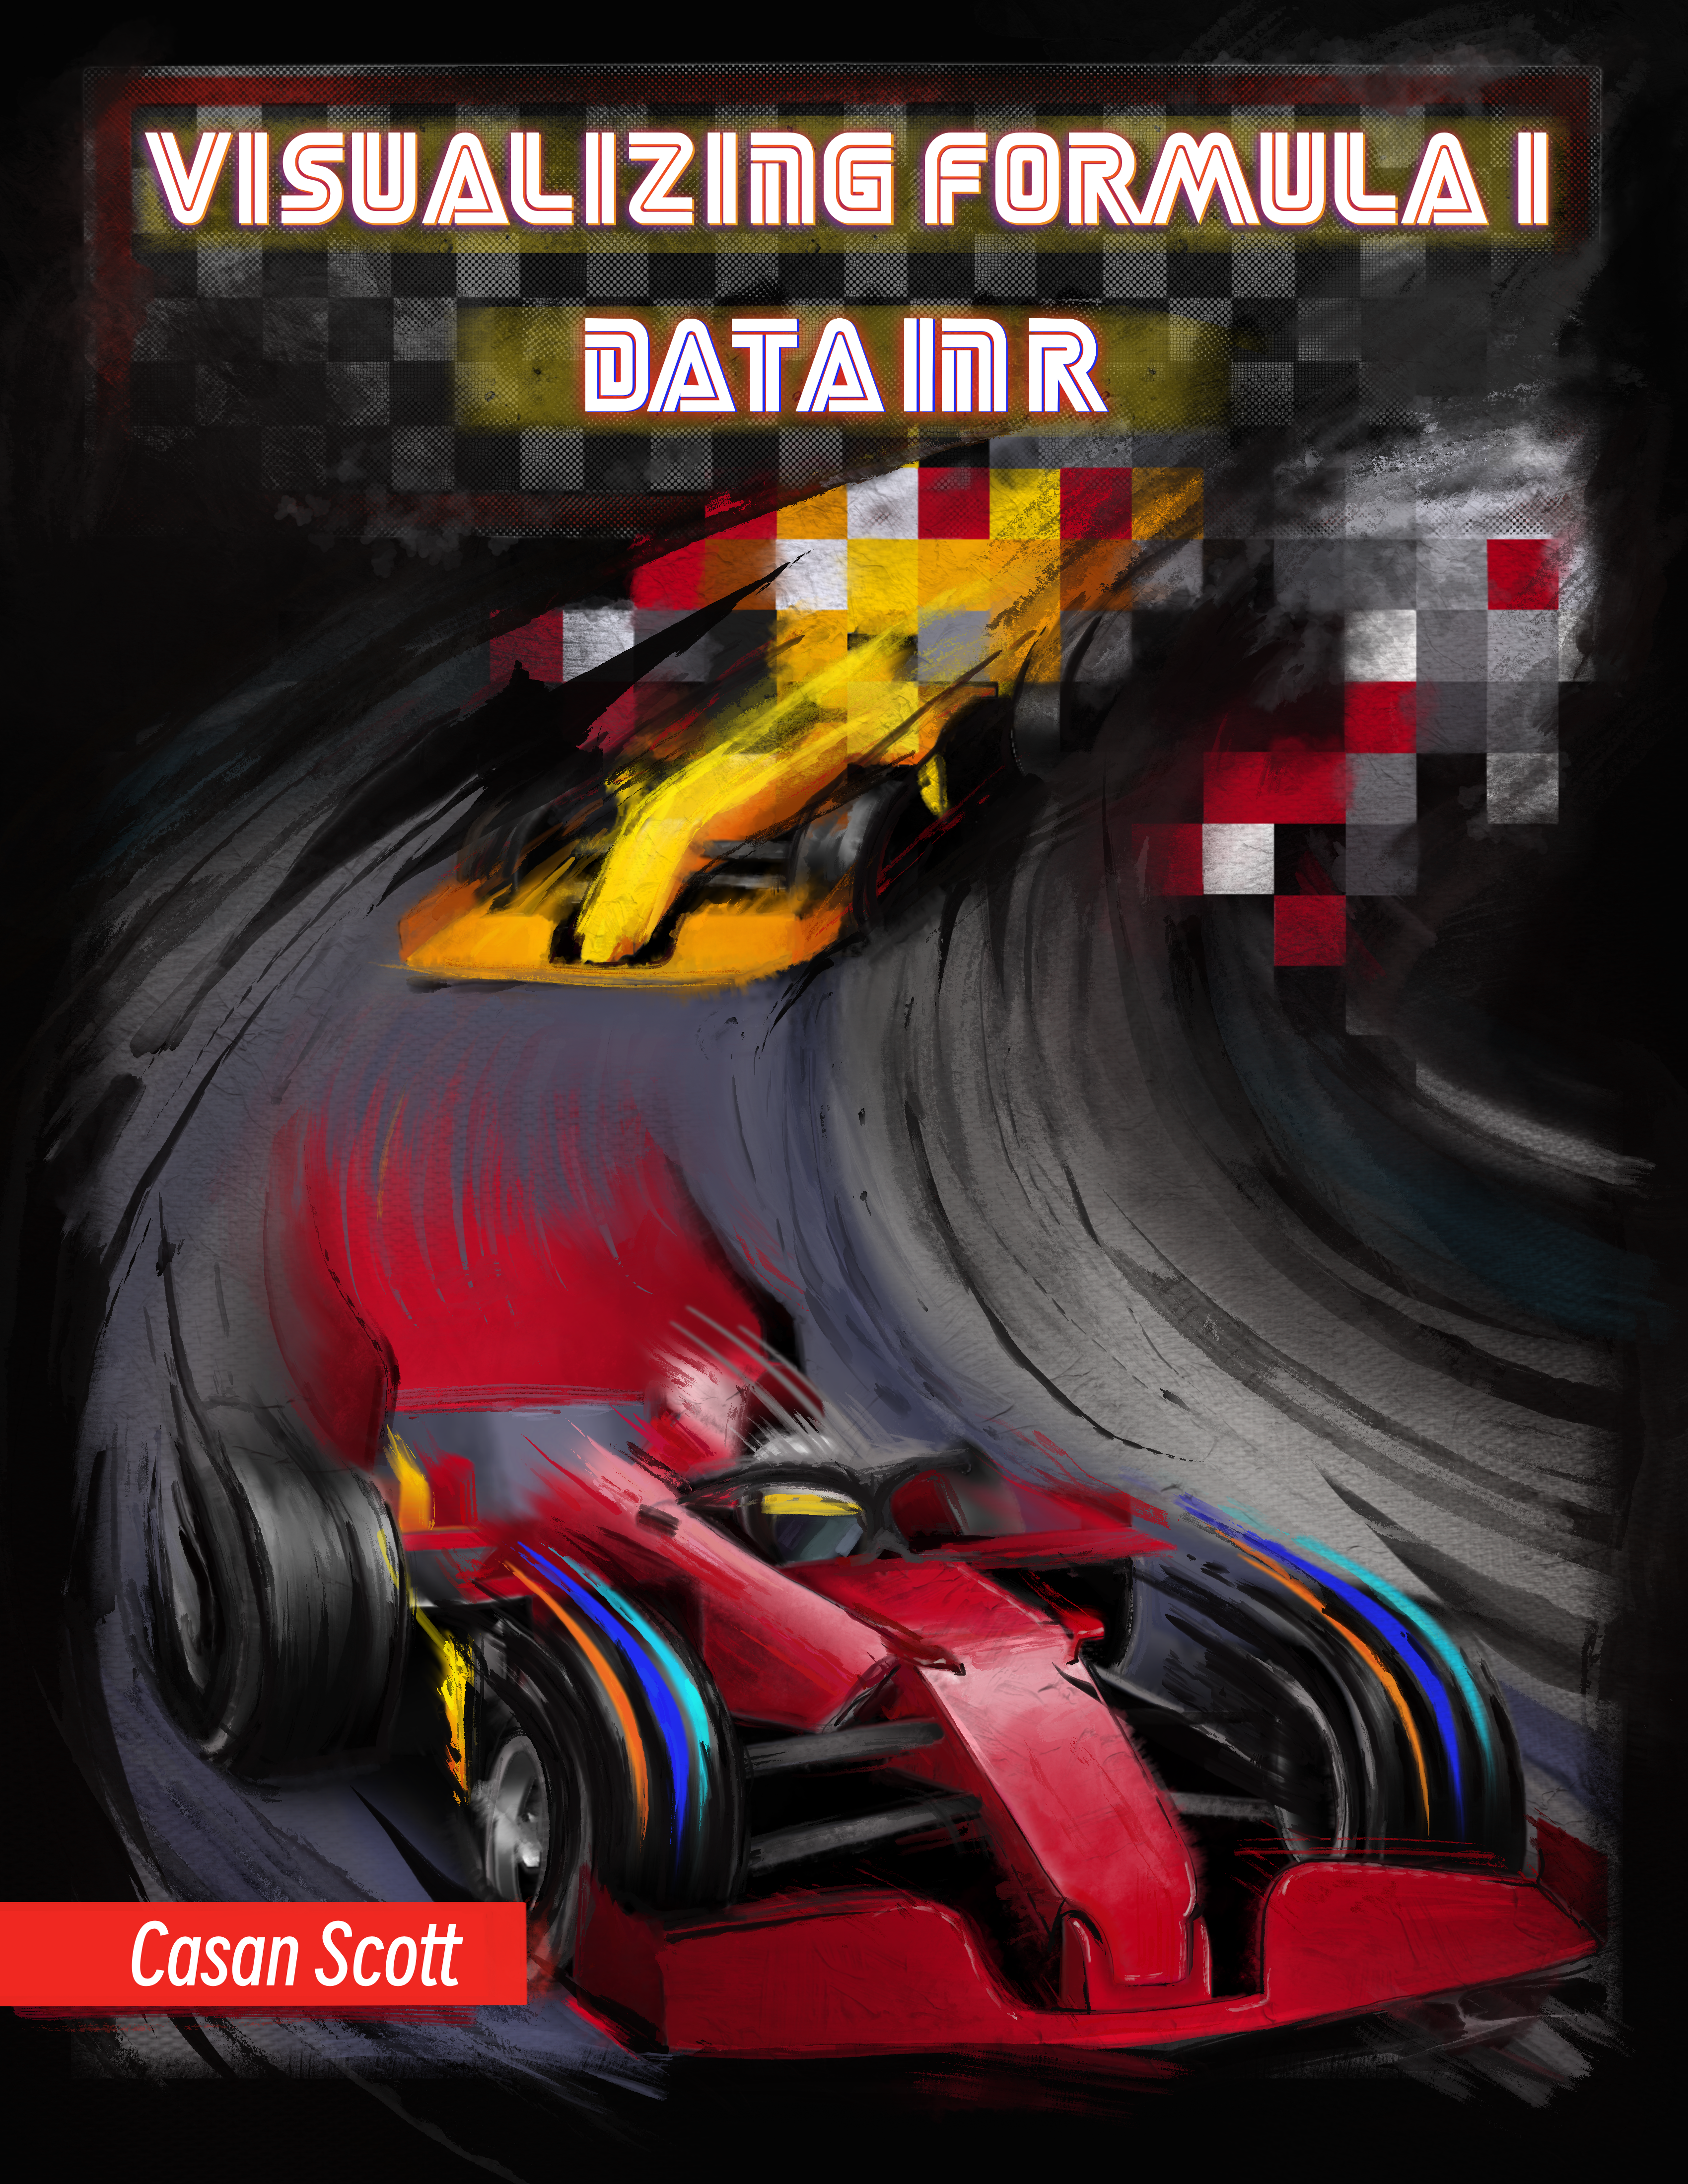
\includegraphics[width=1\linewidth,height=1\textheight]{F1_book_cover} \end{center}

This is a book for anyone that finds themselves located within the fairly obscure intersection of the \emph{data enthusiast-Formula 1 fan} Venn diagram (see Figure below: \protect\hyperlink{Dataux5cux2520Visualization}{1.9 Data Visualization})). This book is \emph{primarily} written for people interested in data visualization using the R programming language, but I hope some of the nerdier Formula 1 fans will also find these data visualizations interesting. In this book, I will do my best to introduce approaches for analyzing Formula 1 data using the R programming language. Along the way, I will also include lots of references and sources for supplemental information.

\newpage

\hypertarget{cover-art}{%
\section{Cover Art}\label{cover-art}}

The cover art is the work of Alison Gaspard. Alison is a tattoo artist, BFA in studio art, and former Visual Arts/Art History educator located in Houston, Texas.

You can find Alison here: \url{https://www.alisonlenayfineart.com/}

\hypertarget{about-me}{%
\section{About me}\label{about-me}}

TLDR: Casan Scott, Ph.D., Senior Data Scientist

More information: I am a bit of a nomad, professionally. Academically, I graduated with B.S. and Ph.D.~degrees in environmental science and my Ph.D.~research focused on the toxicology of fish. Naturally, I decided to \emph{not} use my doctorate degree and became a data scientist! I fell in love with the R programming language during graduate school, and decided I would rather \emph{analyze} data than \emph{collect} it. Over the past five years, I've worked as a data scientist in both the public and private sectors. At times, I also contribute to research on human performance topics. Outside of my nerdier professional pursuits, I enjoy competing in powerlifting, trail running, reading westerns, and hanging out with my wife and dogs.

\hypertarget{why-did-i-write-this-book}{%
\section{Why did I write this book?}\label{why-did-i-write-this-book}}

To scratch my own itch \emph{per se}. Formula 1 is actually a very complicated sport, and while learning about it I had lots of questions: \emph{Do practice times mean anything? Does the qualifying time predict race pace? How much do the cars improve each year? Why is Red Bull so good in Mexico City?} Of course, there were plenty of answers to these questions online, but I really wanted to try and answer some of these questions myself. So, this book documents my attempt at doing so. Along the way, I include the code to create each plot and some brief annotations about the functions used.

\hypertarget{organization-of-this-book}{%
\section{Organization of this book}\label{organization-of-this-book}}

I tried to organize this book like a typical Formula 1 weekend: (1) practice data, (2) qualifying data , and (3) results from the Grand Prix. For the most part, I try to summarize the historical data, visualize possible trends in the data, explore important differences, plot potential correlations, and perhaps build a model that can explain some relationship(s) that seems interesting. Along the way, I may pursue a tangent or two. Each chapter begins with a racing-centric introduction, followed by a data analysis.

\hypertarget{r}{%
\section{R}\label{r}}

R is a programming language that is largely used for statistical analysis and data visualization. One of R's biggest strengths is the ease with which high quality data visualizations can be be produced. This feature is probably what drew me to the language back in 2013, and is the reason that I am able to write this book!

For information on R, visit this link: \url{https://www.r-project.org/about.html}

\hypertarget{ggplot2}{%
\section{ggplot2}\label{ggplot2}}

I am assuming that you have some experience using the R programming language. If you have never used R before, you will quickly become very confused! This entire book is based on the \textbf{ggplot2} package in R. \textbf{ggplot2} is a package used for producing statistical and other data graphics. What makes \textbf{ggplot2} unique, is it has an underlying \emph{grammar}, based on the Grammar of Graphics (Wilkinson 2005). This attribute allows you to create graphs by combining independent components to suit your particular problem. That may seem like a trivial distinction, but it makes \textbf{ggplot2} very powerful!

Note: At times, I may refer to \textbf{ggplot2} as simply \textbf{ggplot}. If that is annoying\ldots{} apologies in advance!

\hypertarget{the-tidyverse}{%
\section{\texorpdfstring{The \emph{tidyverse}}{The tidyverse}}\label{the-tidyverse}}

Throughout this book, I rely on the \textbf{tidyverse}. The \textbf{tidyverse} is actually a collection of other packages that share common data representations and design structures. This enables these packages to work together \emph{very} conveniently. For instance, I nearly always use functions from the \textbf{dplyr} package to wrangle data prior to plotting with \textbf{ggplot2}. You can install the \textbf{tidyverse} core packages with a single command:

\begin{verbatim}
# Install the package from CRAN
install.packages("tidyverse")

# Load the package
library(tidyverse)
\end{verbatim}

The core pakcages in \textbf{tidyverse} are:

\begin{itemize}
\tightlist
\item
  \textbf{ggplot2}, for data visualization.
\item
  \textbf{dplyr}, for data manipulation.
\item
  \textbf{tidyr}, for data tidying.
\item
  \textbf{readr}, for data import.
\item
  \textbf{purrr}, for functional programming.
\item
  \textbf{tibble}, for tibbles, a modern re-imagining of data frames.
\item
  \textbf{stringr}, for strings.
\item
  \textbf{forcats}, for factors.
\item
  \textbf{lubridate}, for date/times.
\end{itemize}

Aside from \textbf{ggplot2}, I most heavily use \textbf{dplyr} in this book. There are six key \textbf{dplyr} functions that can solve most data manipulation challenges:

\begin{itemize}
\tightlist
\item
  \texttt{select()}: subset columns from a dataframe. In other words, you use this to choose variables by name.
\item
  \texttt{filter()}: filter the dataframe by values of a variable. This can be both numeric (i.e.~age \textgreater{} 21 years) or categorical (i.e.~month == June).
\item
  \texttt{arrange()}: order the rows of the dataframe
\item
  \texttt{mutate()}: create a new variable
\item
  \texttt{summarize()}: collapse values down to a summarized metric (i.e.~mean, minimum, maximum).
\item
  \texttt{group\_by()}: operates any of the previous functions on a group basis (i.e.~a grouped mean).
\end{itemize}

I highly recommend this book chapter for more information on \textbf{dplyr} basics:

\url{https://r4ds.had.co.nz/transform.html}

For a thorough introduction to the \textbf{tidyverse}, read the entire fantastic book:

\url{https://r4ds.had.co.nz/index.html}

\hypertarget{data}{%
\section{Data}\label{data}}

The data used in this book was pulled from formula1.com. To make it easier for readers to use this data, I developed the R packaged \textbf{drs} (\textbf{D}ata for \textbf{R}acing \textbf{S}imulations). If you currently follow Formula 1, you'll recognize that DRS also stands for \emph{Drag Reduction System}, which is a crucial component of Formula 1 cars that opens space in the rear wing thereby reducing drag. \textbf{drs} is also an R package that utilizes functions from the \textbf{rvest} and \textbf{dplyr} packages to scrape and tidy data from the formula1.com website. It is designed to scrape data for all Grand Prix weekends during a given year. Each function returns a dataframe that you can then use for analysis and visualizations.

\begin{blackbox}

\begin{center}
\textbf{Notes about a Formula 1 Grand Prix Weekend}

\end{center}

A Grand Prix weekend consists of practice sessions, qualifying, and a race. Additionally, some weekends will also include a sprint race (an abbreviated sprint race that is typically about 1/3 the length of a normal race). A typical Formula 1 weekend begins with three practice sessions. The first two practice sessions (FP1 and FP2) are held on Friday. On Saturday, the third practice session (FP3) is held, followed by Qualifying. Qualifying determines the grid for the race on Sunday. Currently, there are three heats in qualifying (Q1, Q2, and Q3). All cars compete in the first heat (\emph{Q1}), and the top 15 fastest times advance to the 2nd heat, \emph{Q2}. From there, the top 10 fastest times during heat 2 advance to \emph{Q3} (heat 3). The starting grid is determined by a driver's final qualifying position (sans penalties). The race takes place on Sunday.

\end{blackbox}

\textbf{drs} currently consists of four scraping functions:

\begin{itemize}
\tightlist
\item
  \texttt{practice\_session\_scraper()}: Scrapes the best times for a given practice session.
\item
  \texttt{qualifying\_scraper()}: Scrapes the best qualifying times during Q1, Q2, and Q3.
\item
  \texttt{starting\_grid\_scraper()}: Scrapes the final starting grid positions for the Grand Prix.
\item
  \texttt{race\_result\_scraper()()}: Scrapes the race results for a Grand Prix (i.e.~finishing position and total time).
\end{itemize}

\hypertarget{installation-of-drs}{%
\subsubsection{Installation of drs}\label{installation-of-drs}}

You can install the development version of \textbf{drs} here:

\begin{Shaded}
\begin{Highlighting}[]
\FunctionTok{install\_github}\NormalTok{(}\StringTok{"casanscott/drs"}\NormalTok{)}
\end{Highlighting}
\end{Shaded}

\hypertarget{using-the-drs-package}{%
\subsubsection{Using the drs package}\label{using-the-drs-package}}

These functions from \textbf{drs} require both the \textbf{tidyverse} and \textbf{rvest} packages. The \texttt{practice\_session\_scraper()} requires two arguments: \texttt{year} and \texttt{practice\_session\_number}. After loading those libraries, along with \textbf{drs}, you can easily scrape data using a function call like this:

\begin{Shaded}
\begin{Highlighting}[]
\FunctionTok{library}\NormalTok{(tidyverse)}
\FunctionTok{library}\NormalTok{(rvest)}
\FunctionTok{library}\NormalTok{(drs)}

\CommentTok{\# pull FP3 practice data}
\NormalTok{p32022 }\OtherTok{\textless{}{-}} \FunctionTok{practice\_session\_scraper}\NormalTok{(}\DecValTok{2022}\NormalTok{, }\DecValTok{3}\NormalTok{)}

\CommentTok{\# View the first 6 rows}
\FunctionTok{head}\NormalTok{(p32022)}
\end{Highlighting}
\end{Shaded}

\begin{verbatim}
##   Position CarNumber   First       Last Driver                  Car     Time
## 1        1         1     Max Verstappen    VER Red Bull Racing RBPT 1:32.544
## 2        2        16 Charles    Leclerc    LEC              Ferrari 1:32.640
## 3        3        11  Sergio      Perez    PER Red Bull Racing RBPT 1:32.791
## 4        4        63  George    Russell    RUS             Mercedes 1:32.935
## 5        5        55  Carlos      Sainz    SAI              Ferrari 1:33.053
## 6        6        44   Lewis   Hamilton    HAM             Mercedes 1:33.121
##      Race Circuit Year Time_secs
## 1 bahrain bahrain 2022    92.544
## 2 bahrain bahrain 2022    92.640
## 3 bahrain bahrain 2022    92.791
## 4 bahrain bahrain 2022    92.935
## 5 bahrain bahrain 2022    93.053
## 6 bahrain bahrain 2022    93.121
\end{verbatim}

The rest of the \textbf{drs} web scraping functions require a single argument: \texttt{year}.

The following function will scrape all qualifying results from 2022:

\begin{Shaded}
\begin{Highlighting}[]
\CommentTok{\# pull qualifying data}
\NormalTok{quali2022 }\OtherTok{\textless{}{-}} \FunctionTok{qualifying\_scraper}\NormalTok{(}\DecValTok{2022}\NormalTok{)}

\CommentTok{\# View the first 6 rows}
\FunctionTok{head}\NormalTok{(quali2022)}
\end{Highlighting}
\end{Shaded}

\begin{verbatim}
##   Position CarNumber    First       Last Driver                  Car Laps       Q1
## 1        1        16  Charles    Leclerc    LEC              Ferrari   15 1:31.471
## 2        2         1      Max Verstappen    VER Red Bull Racing RBPT   14 1:31.785
## 3        3        55   Carlos      Sainz    SAI              Ferrari   15 1:31.567
## 4        4        11   Sergio      Perez    PER Red Bull Racing RBPT   18 1:32.311
## 5        5        44    Lewis   Hamilton    HAM             Mercedes   17 1:32.285
## 6        6        77 Valtteri     Bottas    BOT   Alfa Romeo Ferrari   15 1:31.919
##         Q2       Q3    Race Circuit Year Q1_secs Q2_secs Q3_secs
## 1 1:30.932 1:30.558 bahrain bahrain 2022  91.471  90.932  90.558
## 2 1:30.757 1:30.681 bahrain bahrain 2022  91.785  90.757  90.681
## 3 1:30.787 1:30.687 bahrain bahrain 2022  91.567  90.787  90.687
## 4 1:31.008 1:30.921 bahrain bahrain 2022  92.311  91.008  90.921
## 5 1:31.048 1:31.238 bahrain bahrain 2022  92.285  91.048  91.238
## 6 1:31.717 1:31.560 bahrain bahrain 2022  91.919  91.717  91.560
\end{verbatim}

To scrape the starting grids for every Grand Prix during 2022, use the following function call:

\begin{Shaded}
\begin{Highlighting}[]
\CommentTok{\# pull starting grids}
\NormalTok{grids2022 }\OtherTok{\textless{}{-}} \FunctionTok{starting\_grid\_scraper}\NormalTok{(}\DecValTok{2022}\NormalTok{)}

\CommentTok{\# View the first 6 rows}
\FunctionTok{head}\NormalTok{(grids2022)}
\end{Highlighting}
\end{Shaded}

\begin{verbatim}
##   Position CarNumber    First       Last Driver                  Car     Time
## 1        1        16  Charles    Leclerc    LEC              Ferrari 1:30.558
## 2        2         1      Max Verstappen    VER Red Bull Racing RBPT 1:30.681
## 3        3        55   Carlos      Sainz    SAI              Ferrari 1:30.687
## 4        4        11   Sergio      Perez    PER Red Bull Racing RBPT 1:30.921
## 5        5        44    Lewis   Hamilton    HAM             Mercedes 1:31.238
## 6        6        77 Valtteri     Bottas    BOT   Alfa Romeo Ferrari 1:31.560
##      Race Circuit Year Time_secs
## 1 bahrain bahrain 2022    90.558
## 2 bahrain bahrain 2022    90.681
## 3 bahrain bahrain 2022    90.687
## 4 bahrain bahrain 2022    90.921
## 5 bahrain bahrain 2022    91.238
## 6 bahrain bahrain 2022    91.560
\end{verbatim}

To scrape the race results for every Grand Prix during 2022, use the following function call:

\begin{Shaded}
\begin{Highlighting}[]
\CommentTok{\# Pull race results}
\NormalTok{races2022 }\OtherTok{\textless{}{-}} \FunctionTok{race\_result\_scraper}\NormalTok{(}\DecValTok{2022}\NormalTok{)}

\CommentTok{\# View the first 6 rows}
\FunctionTok{head}\NormalTok{(races2022)}
\end{Highlighting}
\end{Shaded}

\begin{verbatim}
## # A tibble: 6 x 13
##   Position CarNumber First Last  Driver Car    Laps Time  Points Race  Circuit  Year
##   <chr>        <int> <chr> <chr> <chr>  <chr> <int> <chr>  <int> <chr> <chr>   <dbl>
## 1 1               16 Char~ Lecl~ LEC    Ferr~    57 1:37~     26 bahr~ bahrain  2022
## 2 2               55 Carl~ Sainz SAI    Ferr~    57 +5.5~     18 bahr~ bahrain  2022
## 3 3               44 Lewis Hami~ HAM    Merc~    57 +9.6~     15 bahr~ bahrain  2022
## 4 4               63 Geor~ Russ~ RUS    Merc~    57 +11.~     12 bahr~ bahrain  2022
## 5 5               20 Kevin Magn~ MAG    Haas~    57 +14.~     10 bahr~ bahrain  2022
## 6 6               77 Valt~ Bott~ BOT    Alfa~    57 +16.~      8 bahr~ bahrain  2022
## # i 1 more variable: Time_secs <dbl>
\end{verbatim}

You can then use these dataframes to create cool data visualizations like this one:

\begin{center}\includegraphics{_book/The-book_files/figure-latex/unnamed-chunk-2-1} \end{center}

\hypertarget{data-visualization}{%
\section{Data Visualization}\label{data-visualization}}

In addition to commentary about Formula 1 racing, I'll also include brief instructions about how to create the data visualizations in this book. For example, use this chunk of code\ldots{}

\begin{Shaded}
\begin{Highlighting}[]
\FunctionTok{library}\NormalTok{(ggvenn)}
\FunctionTok{library}\NormalTok{(ggplot2)}

\NormalTok{x }\OtherTok{\textless{}{-}} \FunctionTok{list}\NormalTok{(}\StringTok{\textasciigrave{}}\AttributeTok{Formula 1 fan}\StringTok{\textasciigrave{}} \OtherTok{=} \FunctionTok{rep}\NormalTok{(}\StringTok{\textquotesingle{}This book!\textquotesingle{}}\NormalTok{, }\DecValTok{1}\NormalTok{),}
          \StringTok{\textasciigrave{}}\AttributeTok{Data enthusiast}\StringTok{\textasciigrave{}} \OtherTok{=} \FunctionTok{rep}\NormalTok{(}\StringTok{\textquotesingle{}This book!\textquotesingle{}}\NormalTok{, }\DecValTok{1}\NormalTok{))}


\FunctionTok{ggvenn}\NormalTok{(}
\NormalTok{  x, }
  \AttributeTok{show\_elements =}\NormalTok{ T,}
  \AttributeTok{show\_percentage =}\NormalTok{ F,}
  \AttributeTok{fill\_color =} \FunctionTok{c}\NormalTok{(}\StringTok{"\#CD534CFF"}\NormalTok{, }\StringTok{"\#0073C2FF"}\NormalTok{),}
  \AttributeTok{stroke\_size =} \FloatTok{0.5}\NormalTok{, }\AttributeTok{stroke\_alpha =} \FloatTok{0.5}\NormalTok{, }\AttributeTok{set\_name\_size =} \DecValTok{4}
\NormalTok{  )}
\end{Highlighting}
\end{Shaded}

\ldots{} to create this figure:

\begin{center}\includegraphics{_book/The-book_files/figure-latex/unnamed-chunk-4-1} \end{center}

I'll also occasionally include shaded boxes with supplemental information about a particular chart type, an interesting R package, or anything else that seems noteworthy. For example, the following shaded box includes additional information on the R package used to create the Venn diagram (\textbf{ggvenn}):

\begin{blackbox}

\begin{center}
\textbf{How to create a Venn diagram in R}

\end{center}

I used the \textbf{ggvenn} and \textbf{ggplot2} packages to create this simple Venn diagram. The \textbf{ggvenn} package was created by Linlin Yan. In my opinion, \textbf{ggvenn} is the easiest way to create simple Venn diagrams that follow the typical \textbf{ggplot2} styling and syntax.

For more information about the \textbf{ggvenn} package, visit this link: \url{https://cran.r-project.org/web/packages/ggvenn/index.html}

If you've never used \textbf{ggplot2} before (boy, are you in for a treat!), check out this link to the \textbf{ggplot} book written by legends of the tidyverse Hadley Wickham, Danielle Navarro, and Thomas Lin Pedersen: \url{https://ggplot2-book.org/}

\end{blackbox}

In the next chapter, we will dive into Formula 1 data. I'll start with a gentle introduction to Formula 1 and a typical Grand Prix weekend.

\hypertarget{introduction-to-formula-1}{%
\chapter{Introduction to Formula 1}\label{introduction-to-formula-1}}

What is Formula 1? The word \emph{formula} refers to a particular ruleset that teams' cars must conform to. The numeral \emph{1} designates that this classification is the highest level of motorsport competition. So, \emph{Formula 1} racing is the highest class of international open-wheel single-seater formula racing sanctioned by the Fédération Internationale de l'Automobile (FIA). A Formula 1 season includes a series of \emph{Grands Prix} (races) that take place across the globe on various types of tracks, ranging from closed public city streets to designated racing circuits and modern manufactured street-circuits.

Like many professional sports, Formula 1 is also big business! Thanks in part to the popular Netflix series \emph{Drive to Survive}, Formula has experienced a recent explosion of popularity in the United States (I am one of these recent converts!). Along with this uptick in popularity, Formula 1 teams have also experienced a surge in valuation. To visualize this trend, I will create a bar chart. Prior to creating the bar chart with the \texttt{ggplot()} function, I have to create the dataframe and then reshape to a \emph{longer format} it using the \texttt{pivot\_longer()} function.

\begin{blackbox}

\begin{center}
\textbf{How to pivot data into a longer format in R}

\end{center}

\texttt{pivot\_longer()} \emph{lengthens} data, increasing the number of rows and decreasing the number of columns.

To \emph{widen} the data, use the \texttt{pivot\_wider()} function, which is the inverse transformation.

For more information on \texttt{pivot\_longer()} and \texttt{pivot\_wider()}, visit this link: \url{https://tidyr.tidyverse.org/reference/pivot_longer.html}

\end{blackbox}

The following figure was created using data compiled by \url{https://thesportsdaily.com/}, and originally retrieved from Sportico and Statista:

\begin{Shaded}
\begin{Highlighting}[]
\FunctionTok{library}\NormalTok{(tidyverse)}

\NormalTok{valuation\_table }\OtherTok{\textless{}{-}} \FunctionTok{data.frame}\NormalTok{(}\StringTok{\textasciigrave{}}\AttributeTok{F1 Team}\StringTok{\textasciigrave{}} \OtherTok{=} \FunctionTok{c}\NormalTok{(}\StringTok{\textquotesingle{}Ferrari\textquotesingle{}}\NormalTok{, }\StringTok{\textquotesingle{}Mercedes\textquotesingle{}}\NormalTok{, }\StringTok{\textquotesingle{}Red Bull\textquotesingle{}}\NormalTok{, }\StringTok{\textquotesingle{}McLaren\textquotesingle{}}\NormalTok{, }\StringTok{\textquotesingle{}Aston Martin\textquotesingle{}}\NormalTok{,}
                                            \StringTok{\textquotesingle{}Alpine\textquotesingle{}}\NormalTok{, }\StringTok{\textquotesingle{}Alpha Tauri\textquotesingle{}}\NormalTok{, }\StringTok{\textquotesingle{}Alfa Romeo\textquotesingle{}}\NormalTok{, }\StringTok{\textquotesingle{}Williams\textquotesingle{}}\NormalTok{, }\StringTok{\textquotesingle{}Haas\textquotesingle{}}\NormalTok{),}
                              \StringTok{\textasciigrave{}}\AttributeTok{2018 Valuation}\StringTok{\textasciigrave{}} \OtherTok{=} \FunctionTok{c}\NormalTok{(}\DecValTok{1350}\NormalTok{, }\DecValTok{1015}\NormalTok{, }\DecValTok{640}\NormalTok{, }\DecValTok{620}\NormalTok{, }\ConstantTok{NA}\NormalTok{, }\DecValTok{430}\NormalTok{, }\DecValTok{200}\NormalTok{, }\DecValTok{105}\NormalTok{, }\DecValTok{400}\NormalTok{, }\DecValTok{115}\NormalTok{),}
                              \StringTok{\textasciigrave{}}\AttributeTok{2023 Valuation}\StringTok{\textasciigrave{}} \OtherTok{=} \FunctionTok{c}\NormalTok{(}\DecValTok{3130}\NormalTok{, }\DecValTok{2700}\NormalTok{, }\DecValTok{2420}\NormalTok{, }\DecValTok{1560}\NormalTok{, }\DecValTok{1140}\NormalTok{, }\DecValTok{1080}\NormalTok{, }\DecValTok{905}\NormalTok{, }\DecValTok{815}\NormalTok{, }\DecValTok{795}\NormalTok{, }\DecValTok{710}\NormalTok{)) }\SpecialCharTok{\%\textgreater{}\%}
  \FunctionTok{pivot\_longer}\NormalTok{(}\SpecialCharTok{{-}}\NormalTok{ F1.Team, }\AttributeTok{names\_to =} \StringTok{\textquotesingle{}year\textquotesingle{}}\NormalTok{, }\AttributeTok{values\_to =} \StringTok{\textquotesingle{}valuation\textquotesingle{}}\NormalTok{) }\SpecialCharTok{\%\textgreater{}\%}
  \FunctionTok{mutate}\NormalTok{(}\AttributeTok{year =} \FunctionTok{str\_remove}\NormalTok{(year, }\StringTok{\textquotesingle{}X\textquotesingle{}}\NormalTok{),}
         \AttributeTok{year =} \FunctionTok{str\_remove}\NormalTok{(year, }\StringTok{\textquotesingle{}.Valuation\textquotesingle{}}\NormalTok{))}

\NormalTok{valuation\_table }\SpecialCharTok{\%\textgreater{}\%}
  \FunctionTok{ggplot}\NormalTok{(}\FunctionTok{aes}\NormalTok{(}\AttributeTok{y =} \FunctionTok{fct\_reorder}\NormalTok{(F1.Team, valuation), }\AttributeTok{x =}\NormalTok{ valuation, }\AttributeTok{fill =}\NormalTok{ year)) }\SpecialCharTok{+}
  \FunctionTok{geom\_histogram}\NormalTok{(}\AttributeTok{stat =} \StringTok{\textquotesingle{}identity\textquotesingle{}}\NormalTok{, }\AttributeTok{position =} \StringTok{\textquotesingle{}dodge\textquotesingle{}}\NormalTok{, }\AttributeTok{alpha =} \FloatTok{0.5}\NormalTok{) }\SpecialCharTok{+}
  \FunctionTok{labs}\NormalTok{(}\AttributeTok{title =} \StringTok{\textquotesingle{}Increase in Formula 1 Team Valuations\textquotesingle{}}\NormalTok{,}
       \AttributeTok{subtitle =} \StringTok{\textquotesingle{}2018 vs 2023\textquotesingle{}}\NormalTok{,}
       \AttributeTok{y =} \StringTok{\textquotesingle{}F1 Team\textquotesingle{}}\NormalTok{,}
       \AttributeTok{x =} \StringTok{\textquotesingle{}Valuation (Millions)\textquotesingle{}}\NormalTok{,}
       \AttributeTok{caption =} \StringTok{\textquotesingle{}data sources:  }\SpecialCharTok{\textbackslash{}n}\StringTok{ https://thesportsdaily.com/news/f1{-}teams{-}valuations{-}increase{-}by{-}an{-}average{-}of{-}280{-}over{-}last{-}five{-}years/ }\SpecialCharTok{\textbackslash{}n}\StringTok{ https://www.sportico.com/leagues/motorsports/2023/richest{-}formula{-}1{-}teams{-}most{-}valuable{-}1234727541/ }\SpecialCharTok{\textbackslash{}n}\StringTok{ https://www.sportico.com/leagues/motorsports/2023/richest{-}formula{-}1{-}teams{-}most{-}valuable{-}1234727541/\textquotesingle{}}\NormalTok{) }\SpecialCharTok{+}
  \FunctionTok{theme\_bw}\NormalTok{() }\SpecialCharTok{+}
  \FunctionTok{scale\_x\_continuous}\NormalTok{(}\AttributeTok{labels =}\NormalTok{ scales}\SpecialCharTok{::}\FunctionTok{dollar\_format}\NormalTok{()) }\SpecialCharTok{+}
  \FunctionTok{theme}\NormalTok{(}\AttributeTok{plot.title =} \FunctionTok{element\_text}\NormalTok{(}\AttributeTok{hjust =} \FloatTok{0.5}\NormalTok{),}
        \AttributeTok{plot.subtitle =} \FunctionTok{element\_text}\NormalTok{(}\AttributeTok{hjust =} \FloatTok{0.5}\NormalTok{),}
        \AttributeTok{plot.caption =} \FunctionTok{element\_text}\NormalTok{(}\AttributeTok{hjust =} \DecValTok{0}\NormalTok{, }\AttributeTok{size =} \DecValTok{9}\NormalTok{))}
\end{Highlighting}
\end{Shaded}

\begin{center}\includegraphics{_book/The-book_files/figure-latex/unnamed-chunk-5-1} \end{center}

\begin{blackbox}

\begin{center}
\textbf{How to create a bar chart in R}

\end{center}

To create the figure above, I used the bar geometry, \texttt{geom\_bar()}, in \textbf{ggplot2}. I often use bar charts to plot counts or sums by some grouping variable.

I used two arguments within \texttt{geom\_bar()}: \texttt{stat\ =\ \textquotesingle{}identity\textquotesingle{}} ensures that \textbf{ggplot} uses the dollar sum as listed in the column, while \texttt{position\ =\ \textquotesingle{}dodge\textquotesingle{}} preserves the position along the x-axis.

For more information on \emph{dodging} in \textbf{ggplot2}, visit this link: \url{https://ggplot2.tidyverse.org/reference/position_dodge.html}

\end{blackbox}

Each team has two cars driven by two drivers. Drivers and teams are awarded points based on their finishing position in each Grand Prix. The final tally of points scored will decide two competitions that are taking place during a Formula 1 season: (1) a driver's championship, and (2) a constructors championship (team championship). Currently, Formula 1 has 10 teams, 20 drivers, and awards the following points for each finishing position. Additionally, 1 point is awarded to the driver with the fastest lap during a Grand Prix.

\begin{Shaded}
\begin{Highlighting}[]
\FunctionTok{library}\NormalTok{(tidyverse)}
\FunctionTok{library}\NormalTok{(gt)}
\FunctionTok{library}\NormalTok{(knitr)}

\NormalTok{points\_dataframe }\OtherTok{\textless{}{-}} \FunctionTok{data.frame}\NormalTok{(}\AttributeTok{Placing =} \FunctionTok{c}\NormalTok{(}\StringTok{\textquotesingle{}1\textquotesingle{}}\NormalTok{, }\StringTok{\textquotesingle{}2\textquotesingle{}}\NormalTok{, }\StringTok{\textquotesingle{}3\textquotesingle{}}\NormalTok{, }\StringTok{\textquotesingle{}4\textquotesingle{}}\NormalTok{, }\StringTok{\textquotesingle{}5\textquotesingle{}}\NormalTok{, }\StringTok{\textquotesingle{}6\textquotesingle{}}\NormalTok{, }\StringTok{\textquotesingle{}7\textquotesingle{}}\NormalTok{, }\StringTok{\textquotesingle{}8\textquotesingle{}}\NormalTok{, }\StringTok{\textquotesingle{}9\textquotesingle{}}\NormalTok{, }\StringTok{\textquotesingle{}10\textquotesingle{}}\NormalTok{, }\StringTok{\textquotesingle{}11 {-} 20\textquotesingle{}}\NormalTok{),}
           \AttributeTok{Pts =} \FunctionTok{c}\NormalTok{(}\DecValTok{25}\NormalTok{, }\DecValTok{18}\NormalTok{, }\DecValTok{15}\NormalTok{, }\DecValTok{12}\NormalTok{, }\DecValTok{10}\NormalTok{, }\DecValTok{8}\NormalTok{, }\DecValTok{6}\NormalTok{, }\DecValTok{4}\NormalTok{, }\DecValTok{2}\NormalTok{, }\DecValTok{1}\NormalTok{, }\DecValTok{0}\NormalTok{))}

\FunctionTok{gt}\NormalTok{(points\_dataframe)  }\SpecialCharTok{\%\textgreater{}\%} 
  \FunctionTok{cols\_align}\NormalTok{(}\AttributeTok{align =} \FunctionTok{c}\NormalTok{(}\StringTok{"center"}\NormalTok{), }\AttributeTok{columns =} \DecValTok{2}\NormalTok{) }\SpecialCharTok{\%\textgreater{}\%} 
  \FunctionTok{tab\_options}\NormalTok{(}\AttributeTok{column\_labels.font.weight =} \StringTok{"bold"}\NormalTok{)}
\end{Highlighting}
\end{Shaded}

\begin{longtable}{rc}
\toprule
Placing & Pts \\ 
\midrule
1 & 25 \\ 
2 & 18 \\ 
3 & 15 \\ 
4 & 12 \\ 
5 & 10 \\ 
6 & 8 \\ 
7 & 6 \\ 
8 & 4 \\ 
9 & 2 \\ 
10 & 1 \\ 
11 - 20 & 0 \\ 
\bottomrule
\end{longtable}

\begin{blackbox}

\begin{center}
\textbf{How to create a table in R}

\end{center}

To create the table above, I simply pipe (i.e.~\texttt{\%\textgreater{}\%}) a manually-created dataframe to the \texttt{gt()} function (i.e.~\texttt{df\ \%\textgreater{}\%\ gt()}). The \texttt{gt()} function is found in the \textbf{gt} package. The \textbf{gt} package is the best way (in my opinion!) to create beautiful tables using the R programming language. \textbf{gt} functions work great with dataframes and tibbles, and can easily become an extension of yur typical tidy workflow. This example above is an absolute bare-bones examples of a \textbf{gt} table.

Another way to create this type of table would be to use the \texttt{kable()} function from the \textbf{knitr} package. The \texttt{kable()} function is a very simple table generator in R.

For more information about the \textbf{gt} package, visit this link:

\url{https://gt.rstudio.com/}

This guide provides lots of information about styling aesthetics of a table, including table headers and footers, column labels, and much, much more!

\end{blackbox}

\hypertarget{data-1}{%
\section{Data}\label{data-1}}

In this book, I will limit the data to include only years 2014 through 2023. Why start in 2014? 2014 marks the beginning of the \textbf{turbo-hybrid} era in Formula 1. In 2014, F1 made perhaps the most significant rule change it its' history by replacing normally aspirated V8 engines with 1.6 liter turbocharged V6 engines. In fact, F1 engines are now actually referred to as \emph{power units}. This new set of regulations seemed like an ideal place to start my analyses. At times in this book, I will note changes occurring after the 2021 season. I do this because 2022 marked another year of significant change in the regulations, this time aerodynamically. After a forty-year ban, \textbf{ground effect} returned to Formula 1. The goal for a Formula 1 design team is to optimize ground effect so that the bottom of the car generates low pressure, which will \emph{suck} the car to the track. This new set of regulations in 2022 disrupted Mercedes period of dominance from 2014 to 2021.

\hypertarget{a-formula-1-weekend}{%
\section{A Formula 1 Weekend}\label{a-formula-1-weekend}}

A Formula One Grand Prix is actually not just a single race, but rather a sporting event spanning three days, typically from Friday to Sunday. Beginning on Friday, there is typically two practices (\textbf{FP1} and \textbf{FP2}), followed by a third practice (\textbf{FP3}) and a qualifying session on Saturday. Practice sessions provide teams an opportunity to \emph{practice} on the circuit, and experiment with the setup of the car. Qualifying determines the grid for the race on Sunday. Currently, there are three heats in qualifying. All cars compete in the first heat (\textbf{Q1}), and the top 15 fastest times advance to the 2nd heat (\textbf{Q2}). From there, the top 10 fastest times during heat 2 advance to \emph{Q3} (heat 3). Qualifying times determine the starting grid for the Grand Prix. The fastest qualifying times start the race at the front of the \emph{grid}, and the slowest start at the back. If a driver incurs a penalty during qualifying, the starting grid will be adjusted accordingly. The race takes place on Sunday, and the top three placed drivers take their places upon a \emph{podium}.

\hypertarget{practice-sessions}{%
\section{Practice Sessions}\label{practice-sessions}}

Currently, there are three free practice sessions (often abbreviated to FP1, FP2, and FP3) that are held before the race. The first (FP1) is held on Friday morning, the second (FP2) on Friday afternoon, and the third session (FP3) is held on Saturday morning. Since 2021, practice sessions last for one hour, but previously Friday sessions were 90 minutes long.

Typically, teams will use each practice session for a different purpose. For instance, FP1 is often used to test the car and ensure it is working as expected, while also collecting information on the track and car setup. FP2 is often used for additional reconnaissance and testing of the car's performance on \emph{long runs}. FP3 is most commonly used to understand the car's speed over lap (i.e.~qualifying pace).

When I first became interested in Formula 1, I had tons of questions about the cars, racing, and structure of the Grand Prix weekend. While there are countless resources available to learn about Formula (shout out to r/formula1), I particularly enjoy learning by exploring data. Luckily, you can find practice, qualifying, and Grand Prix data on \url{https://formula1.com/}. To make that data a little more accessible, feel free to use the \texttt{practice\_session\_scraper()} function from my \textbf{drs} package.

To scrape FP1 data for 2014 through 2023, use the following code:

\begin{Shaded}
\begin{Highlighting}[]
\CommentTok{\# Scrape FP1 data}
\NormalTok{fp1\_2023 }\OtherTok{\textless{}{-}} \FunctionTok{practice\_session\_scraper}\NormalTok{(}\DecValTok{2023}\NormalTok{, }\DecValTok{1}\NormalTok{)}
\NormalTok{fp1\_2022 }\OtherTok{\textless{}{-}} \FunctionTok{practice\_session\_scraper}\NormalTok{(}\DecValTok{2022}\NormalTok{, }\DecValTok{1}\NormalTok{)}
\NormalTok{fp1\_2021 }\OtherTok{\textless{}{-}} \FunctionTok{practice\_session\_scraper}\NormalTok{(}\DecValTok{2021}\NormalTok{, }\DecValTok{1}\NormalTok{)}
\NormalTok{fp1\_2020 }\OtherTok{\textless{}{-}} \FunctionTok{practice\_session\_scraper}\NormalTok{(}\DecValTok{2020}\NormalTok{, }\DecValTok{1}\NormalTok{)}
\NormalTok{fp1\_2019 }\OtherTok{\textless{}{-}} \FunctionTok{practice\_session\_scraper}\NormalTok{(}\DecValTok{2019}\NormalTok{, }\DecValTok{1}\NormalTok{)}
\NormalTok{fp1\_2018 }\OtherTok{\textless{}{-}} \FunctionTok{practice\_session\_scraper}\NormalTok{(}\DecValTok{2018}\NormalTok{, }\DecValTok{1}\NormalTok{)}
\NormalTok{fp1\_2017 }\OtherTok{\textless{}{-}} \FunctionTok{practice\_session\_scraper}\NormalTok{(}\DecValTok{2017}\NormalTok{, }\DecValTok{1}\NormalTok{)}
\NormalTok{fp1\_2016 }\OtherTok{\textless{}{-}} \FunctionTok{practice\_session\_scraper}\NormalTok{(}\DecValTok{2016}\NormalTok{, }\DecValTok{1}\NormalTok{)}
\NormalTok{fp1\_2015 }\OtherTok{\textless{}{-}} \FunctionTok{practice\_session\_scraper}\NormalTok{(}\DecValTok{2015}\NormalTok{, }\DecValTok{1}\NormalTok{)}
\NormalTok{fp1\_2014 }\OtherTok{\textless{}{-}} \FunctionTok{practice\_session\_scraper}\NormalTok{(}\DecValTok{2014}\NormalTok{, }\DecValTok{1}\NormalTok{)}
\end{Highlighting}
\end{Shaded}

To scrape FP2 data for the same time period, use this code:

\begin{Shaded}
\begin{Highlighting}[]
\CommentTok{\# Scrape FP2 data}
\NormalTok{fp2\_2023 }\OtherTok{\textless{}{-}} \FunctionTok{practice\_session\_scraper}\NormalTok{(}\DecValTok{2023}\NormalTok{, }\DecValTok{2}\NormalTok{)}
\NormalTok{fp2\_2022 }\OtherTok{\textless{}{-}} \FunctionTok{practice\_session\_scraper}\NormalTok{(}\DecValTok{2022}\NormalTok{, }\DecValTok{2}\NormalTok{)}
\NormalTok{fp2\_2021 }\OtherTok{\textless{}{-}} \FunctionTok{practice\_session\_scraper}\NormalTok{(}\DecValTok{2021}\NormalTok{, }\DecValTok{2}\NormalTok{)}
\NormalTok{fp2\_2020 }\OtherTok{\textless{}{-}} \FunctionTok{practice\_session\_scraper}\NormalTok{(}\DecValTok{2020}\NormalTok{, }\DecValTok{2}\NormalTok{)}
\NormalTok{fp2\_2019 }\OtherTok{\textless{}{-}} \FunctionTok{practice\_session\_scraper}\NormalTok{(}\DecValTok{2019}\NormalTok{, }\DecValTok{2}\NormalTok{)}
\NormalTok{fp2\_2018 }\OtherTok{\textless{}{-}} \FunctionTok{practice\_session\_scraper}\NormalTok{(}\DecValTok{2018}\NormalTok{, }\DecValTok{2}\NormalTok{)}
\NormalTok{fp2\_2017 }\OtherTok{\textless{}{-}} \FunctionTok{practice\_session\_scraper}\NormalTok{(}\DecValTok{2017}\NormalTok{, }\DecValTok{2}\NormalTok{)}
\NormalTok{fp2\_2016 }\OtherTok{\textless{}{-}} \FunctionTok{practice\_session\_scraper}\NormalTok{(}\DecValTok{2016}\NormalTok{, }\DecValTok{2}\NormalTok{)}
\NormalTok{fp2\_2015 }\OtherTok{\textless{}{-}} \FunctionTok{practice\_session\_scraper}\NormalTok{(}\DecValTok{2015}\NormalTok{, }\DecValTok{2}\NormalTok{)}
\NormalTok{fp2\_2014 }\OtherTok{\textless{}{-}} \FunctionTok{practice\_session\_scraper}\NormalTok{(}\DecValTok{2014}\NormalTok{, }\DecValTok{2}\NormalTok{)}
\end{Highlighting}
\end{Shaded}

And finally, to scrape FP3 data, use this:

\begin{Shaded}
\begin{Highlighting}[]
\CommentTok{\# Scrape FP3 data}
\NormalTok{fp3\_2023 }\OtherTok{\textless{}{-}} \FunctionTok{practice\_session\_scraper}\NormalTok{(}\DecValTok{2023}\NormalTok{, }\DecValTok{3}\NormalTok{)}
\NormalTok{fp3\_2022 }\OtherTok{\textless{}{-}} \FunctionTok{practice\_session\_scraper}\NormalTok{(}\DecValTok{2022}\NormalTok{, }\DecValTok{3}\NormalTok{)}
\NormalTok{fp3\_2021 }\OtherTok{\textless{}{-}} \FunctionTok{practice\_session\_scraper}\NormalTok{(}\DecValTok{2021}\NormalTok{, }\DecValTok{3}\NormalTok{)}
\NormalTok{fp3\_2020 }\OtherTok{\textless{}{-}} \FunctionTok{practice\_session\_scraper}\NormalTok{(}\DecValTok{2020}\NormalTok{, }\DecValTok{3}\NormalTok{)}
\NormalTok{fp3\_2019 }\OtherTok{\textless{}{-}} \FunctionTok{practice\_session\_scraper}\NormalTok{(}\DecValTok{2019}\NormalTok{, }\DecValTok{3}\NormalTok{)}
\NormalTok{fp3\_2018 }\OtherTok{\textless{}{-}} \FunctionTok{practice\_session\_scraper}\NormalTok{(}\DecValTok{2018}\NormalTok{, }\DecValTok{3}\NormalTok{)}
\NormalTok{fp3\_2017 }\OtherTok{\textless{}{-}} \FunctionTok{practice\_session\_scraper}\NormalTok{(}\DecValTok{2017}\NormalTok{, }\DecValTok{3}\NormalTok{)}
\NormalTok{fp3\_2016 }\OtherTok{\textless{}{-}} \FunctionTok{practice\_session\_scraper}\NormalTok{(}\DecValTok{2016}\NormalTok{, }\DecValTok{3}\NormalTok{)}
\NormalTok{fp3\_2015 }\OtherTok{\textless{}{-}} \FunctionTok{practice\_session\_scraper}\NormalTok{(}\DecValTok{2015}\NormalTok{, }\DecValTok{3}\NormalTok{)}
\NormalTok{fp3\_2014 }\OtherTok{\textless{}{-}} \FunctionTok{practice\_session\_scraper}\NormalTok{(}\DecValTok{2014}\NormalTok{, }\DecValTok{3}\NormalTok{)}
\end{Highlighting}
\end{Shaded}

Now that the data is scraped from www.formula1.com, I need to combine them together into one dataframe. I will use the \texttt{rbind()} function to row-bind data for each practice session.

\begin{blackbox}

\begin{center}
\textbf{How to bind data in R}

\end{center}

The \texttt{cbind()} and \texttt{rbind()} functions combine by columns or rows, respectively.

For more information on these two functions, visit this link: \url{https://www.rdocumentation.org/packages/base/versions/3.6.2/topics/cbind}

\end{blackbox}

\begin{Shaded}
\begin{Highlighting}[]
\CommentTok{\#Combine all practice data}
\NormalTok{practice\_times }\OtherTok{\textless{}{-}} \FunctionTok{rbind}\NormalTok{(fp3\_2023,}
\NormalTok{                        fp3\_2022,}
\NormalTok{                            fp3\_2021,}
\NormalTok{                            fp3\_2020,}
\NormalTok{                            fp3\_2019,}
\NormalTok{                            fp3\_2018,}
\NormalTok{                            fp3\_2017,}
\NormalTok{                            fp3\_2016,}
\NormalTok{                            fp3\_2015,}
\NormalTok{                            fp3\_2014) }\SpecialCharTok{\%\textgreater{}\%}
  \FunctionTok{left\_join}\NormalTok{(}\FunctionTok{rbind}\NormalTok{(fp2\_2023,}
\NormalTok{                  fp2\_2022,}
\NormalTok{                            fp2\_2021,}
\NormalTok{                            fp2\_2020,}
\NormalTok{                            fp2\_2019,}
\NormalTok{                            fp2\_2018,}
\NormalTok{                            fp2\_2017,}
\NormalTok{                            fp2\_2016,}
\NormalTok{                            fp2\_2015,}
\NormalTok{                            fp2\_2014) }\SpecialCharTok{\%\textgreater{}\%}
\NormalTok{              dplyr}\SpecialCharTok{::}\FunctionTok{select}\NormalTok{(}\StringTok{\textquotesingle{}Driver\textquotesingle{}}\NormalTok{, }\StringTok{\textquotesingle{}Race\textquotesingle{}}\NormalTok{, }\StringTok{\textquotesingle{}Year\textquotesingle{}}\NormalTok{, }\StringTok{\textquotesingle{}Time\textquotesingle{}}\NormalTok{, }\StringTok{\textquotesingle{}Time\_secs\textquotesingle{}}\NormalTok{), }\AttributeTok{by =} \FunctionTok{c}\NormalTok{(}\StringTok{\textquotesingle{}Driver\textquotesingle{}}\NormalTok{, }\StringTok{\textquotesingle{}Race\textquotesingle{}}\NormalTok{, }\StringTok{\textquotesingle{}Year\textquotesingle{}}\NormalTok{), }\AttributeTok{suffix =} \FunctionTok{c}\NormalTok{(}\StringTok{"\_3"}\NormalTok{, }\StringTok{"\_2"}\NormalTok{)) }\SpecialCharTok{\%\textgreater{}\%}
  \FunctionTok{left\_join}\NormalTok{(}\FunctionTok{rbind}\NormalTok{(fp1\_2023,}
\NormalTok{                  fp1\_2022,}
\NormalTok{                            fp1\_2021,}
\NormalTok{                            fp1\_2020,}
\NormalTok{                            fp1\_2019,}
\NormalTok{                            fp1\_2018,}
\NormalTok{                            fp1\_2017,}
\NormalTok{                            fp1\_2016,}
\NormalTok{                            fp1\_2015,}
\NormalTok{                            fp1\_2014) }\SpecialCharTok{\%\textgreater{}\%}
\NormalTok{              dplyr}\SpecialCharTok{::}\FunctionTok{select}\NormalTok{(}\StringTok{\textquotesingle{}Driver\textquotesingle{}}\NormalTok{, }\StringTok{\textquotesingle{}Race\textquotesingle{}}\NormalTok{, }\StringTok{\textquotesingle{}Year\textquotesingle{}}\NormalTok{, }\StringTok{\textquotesingle{}Time\textquotesingle{}}\NormalTok{, }\StringTok{\textquotesingle{}Time\_secs\textquotesingle{}}\NormalTok{), }\AttributeTok{by =} \FunctionTok{c}\NormalTok{(}\StringTok{\textquotesingle{}Driver\textquotesingle{}}\NormalTok{, }\StringTok{\textquotesingle{}Race\textquotesingle{}}\NormalTok{, }\StringTok{\textquotesingle{}Year\textquotesingle{}}\NormalTok{)) }\SpecialCharTok{\%\textgreater{}\%}
  \FunctionTok{rename}\NormalTok{(}\AttributeTok{Time\_1 =}\NormalTok{ Time, }\AttributeTok{Time\_secs\_1 =}\NormalTok{ Time\_secs) }\SpecialCharTok{\%\textgreater{}\%} 
  \FunctionTok{relocate}\NormalTok{(Time\_3, }\AttributeTok{.after =}\NormalTok{ Year)}
\end{Highlighting}
\end{Shaded}

One of my early questions was: \emph{Do cars get faster with each practice session?}

To begin exploring this question, I will initially focus on 2023 practice data.

I can use \texttt{left\_join()} from the \textbf{dplyr} package to merge all practice sessions for the 2023 season.

\begin{Shaded}
\begin{Highlighting}[]
\CommentTok{\# Pull 2023 data}
\CommentTok{\# Scrape FP1 data}
\NormalTok{fp1\_2023 }\OtherTok{\textless{}{-}} \FunctionTok{practice\_session\_scraper}\NormalTok{(}\DecValTok{2023}\NormalTok{, }\DecValTok{1}\NormalTok{)}
\CommentTok{\# Scrape FP2 data}
\NormalTok{fp2\_2023 }\OtherTok{\textless{}{-}} \FunctionTok{practice\_session\_scraper}\NormalTok{(}\DecValTok{2023}\NormalTok{, }\DecValTok{2}\NormalTok{)}
\CommentTok{\# Scrape FP2 data}
\NormalTok{fp3\_2023 }\OtherTok{\textless{}{-}} \FunctionTok{practice\_session\_scraper}\NormalTok{(}\DecValTok{2023}\NormalTok{, }\DecValTok{3}\NormalTok{)}

\CommentTok{\# Merge Practices times for 2022}
\NormalTok{practice\_times\_2023 }\OtherTok{\textless{}{-}}\NormalTok{ fp3\_2023 }\SpecialCharTok{\%\textgreater{}\%}
  \FunctionTok{left\_join}\NormalTok{(fp2\_2023 }\SpecialCharTok{\%\textgreater{}\%}
\NormalTok{              dplyr}\SpecialCharTok{::}\FunctionTok{select}\NormalTok{(}\StringTok{\textquotesingle{}Driver\textquotesingle{}}\NormalTok{, }\StringTok{\textquotesingle{}Race\textquotesingle{}}\NormalTok{, }\StringTok{\textquotesingle{}Year\textquotesingle{}}\NormalTok{, }\StringTok{\textquotesingle{}Time\textquotesingle{}}\NormalTok{, }\StringTok{\textquotesingle{}Time\_secs\textquotesingle{}}\NormalTok{), }\AttributeTok{by =} \FunctionTok{c}\NormalTok{(}\StringTok{\textquotesingle{}Driver\textquotesingle{}}\NormalTok{, }\StringTok{\textquotesingle{}Race\textquotesingle{}}\NormalTok{, }\StringTok{\textquotesingle{}Year\textquotesingle{}}\NormalTok{), }\AttributeTok{suffix =} \FunctionTok{c}\NormalTok{(}\StringTok{"\_3"}\NormalTok{, }\StringTok{"\_2"}\NormalTok{)) }\SpecialCharTok{\%\textgreater{}\%}
  \FunctionTok{left\_join}\NormalTok{(fp1\_2023 }\SpecialCharTok{\%\textgreater{}\%}
\NormalTok{              dplyr}\SpecialCharTok{::}\FunctionTok{select}\NormalTok{(}\StringTok{\textquotesingle{}Driver\textquotesingle{}}\NormalTok{, }\StringTok{\textquotesingle{}Race\textquotesingle{}}\NormalTok{, }\StringTok{\textquotesingle{}Year\textquotesingle{}}\NormalTok{, }\StringTok{\textquotesingle{}Time\textquotesingle{}}\NormalTok{, }\StringTok{\textquotesingle{}Time\_secs\textquotesingle{}}\NormalTok{), }\AttributeTok{by =} \FunctionTok{c}\NormalTok{(}\StringTok{\textquotesingle{}Driver\textquotesingle{}}\NormalTok{, }\StringTok{\textquotesingle{}Race\textquotesingle{}}\NormalTok{, }\StringTok{\textquotesingle{}Year\textquotesingle{}}\NormalTok{)) }\SpecialCharTok{\%\textgreater{}\%}
  \FunctionTok{rename}\NormalTok{(}\AttributeTok{Time\_1 =}\NormalTok{ Time, }\AttributeTok{Time\_secs\_1 =}\NormalTok{ Time\_secs) }\SpecialCharTok{\%\textgreater{}\%} 
  \FunctionTok{relocate}\NormalTok{(Time\_3, }\AttributeTok{.after =}\NormalTok{ Year)}
\end{Highlighting}
\end{Shaded}

\begin{blackbox}

\begin{center}
\textbf{How to join data in R}

\end{center}

Joining data is pretty simple using functions from the \textbf{dplyr} package. In dplyr, you will be mutating joins, which adds columns from y to x, matching observations based on the keys. There are four mutating joins:

\begin{itemize}
\tightlist
\item
  \texttt{inner\_join()}
\item
  \texttt{left\_join()}
\item
  \texttt{right\_join()}
\item
  \texttt{full\_join()}
\end{itemize}

For more information on mutating joins in \textbf{dplyr}, visit this link: \url{https://dplyr.tidyverse.org/reference/mutate-joins.html}

\end{blackbox}

Here's a nother tip on reordering columns:

\begin{blackbox}

\begin{center}
\textbf{How to relocate a column of a dataframe in R}

\end{center}

Notice that in the final line of the above code, I used the \texttt{relocate()} function to reorder a column. This is not necessary, but can help keep your dataframe more organized.

As an example, you could use the following code to move column A after column C in a dataframe:

\texttt{df\ \%\textgreater{}\%\ relocate(a,\ .after\ =\ c)}

For more information on the \texttt{relocate()} function in \textbf{dplyr}, visit this link: \url{https://dplyr.tidyverse.org/reference/relocate.html}

\end{blackbox}

I used the following code to plot the average times by practice session in 2023.

\begin{Shaded}
\begin{Highlighting}[]
\NormalTok{practice\_times\_2023 }\SpecialCharTok{\%\textgreater{}\%}
\NormalTok{  dplyr}\SpecialCharTok{::}\FunctionTok{select}\NormalTok{(Time\_secs\_3, Time\_secs\_2, Time\_secs\_1) }\SpecialCharTok{\%\textgreater{}\%}
  \FunctionTok{pivot\_longer}\NormalTok{(}\FunctionTok{c}\NormalTok{(Time\_secs\_3, Time\_secs\_2, Time\_secs\_1), }\AttributeTok{names\_to =} \StringTok{\textquotesingle{}practice\_session\textquotesingle{}}\NormalTok{, }\AttributeTok{values\_to =} \StringTok{\textquotesingle{}time\textquotesingle{}}\NormalTok{) }\SpecialCharTok{\%\textgreater{}\%}
  \FunctionTok{mutate}\NormalTok{(}\AttributeTok{practice\_session =} \FunctionTok{str\_remove}\NormalTok{(practice\_session, }\StringTok{\textquotesingle{}Time\_secs\_\textquotesingle{}}\NormalTok{)) }\SpecialCharTok{\%\textgreater{}\%}
  \FunctionTok{ggplot}\NormalTok{(}\FunctionTok{aes}\NormalTok{(practice\_session, time)) }\SpecialCharTok{+}
  \FunctionTok{stat\_summary}\NormalTok{(}\AttributeTok{fun.y =}\NormalTok{ mean, }
               \AttributeTok{geom =} \StringTok{"point"}\NormalTok{, }\AttributeTok{pch =} \DecValTok{21}\NormalTok{, }\AttributeTok{col =} \StringTok{\textquotesingle{}black\textquotesingle{}}\NormalTok{, }\AttributeTok{fill =}  \StringTok{\textquotesingle{}red\textquotesingle{}}\NormalTok{, }\AttributeTok{alpha =} \FloatTok{0.5}\NormalTok{, }\AttributeTok{size =} \DecValTok{3}\NormalTok{) }\SpecialCharTok{+} 
  \FunctionTok{theme\_bw}\NormalTok{() }\SpecialCharTok{+}
  \FunctionTok{labs}\NormalTok{(}\AttributeTok{y =} \StringTok{\textquotesingle{}Best Lap Time (secs)\textquotesingle{}}\NormalTok{,}
       \AttributeTok{x =} \StringTok{\textquotesingle{}Practice Session\textquotesingle{}}\NormalTok{,}
       \AttributeTok{title =} \StringTok{\textquotesingle{}Average Best Lap Time by Practice Session\textquotesingle{}}\NormalTok{,}
       \AttributeTok{subtitle =} \StringTok{\textquotesingle{}All Grands Prix: 2023\textquotesingle{}}\NormalTok{) }\SpecialCharTok{+}
  \FunctionTok{theme}\NormalTok{(}\AttributeTok{plot.title =} \FunctionTok{element\_text}\NormalTok{(}\AttributeTok{hjust =} \FloatTok{0.5}\NormalTok{),}
        \AttributeTok{plot.subtitle =} \FunctionTok{element\_text}\NormalTok{(}\AttributeTok{hjust =} \FloatTok{0.5}\NormalTok{))}
\end{Highlighting}
\end{Shaded}

\begin{center}\includegraphics{_book/The-book_files/figure-latex/unnamed-chunk-13-1} \end{center}

\begin{blackbox}

\begin{center}
\textbf{How to create a categorical scatter plot with a computed mean in R}

\end{center}

If there are many observations per group, you can use the \texttt{stat\_summary()} function to calculate a grouped mean of the variable plotted along the y-axis. Specifically, the argument \texttt{fun.y\ =\ mean} specifies that you want to calculate the mean of the y-axis variable. If you wish to \emph{only} plot the mean, include the \texttt{geom\ =\ "point"} argument.

For more information on \texttt{stat\_summary()} in \textbf{ggplot2}, visit this link: \url{https://ggplot2.tidyverse.org/reference/stat_summary.html}

\end{blackbox}

When pooling all teams, drivers, and circuits together, it looks like the average time during P1 is slower than both P2 and P3. P3's average time is slightly slower than P2. But, these times will obviously vary considerably by year, Grand Prix, team, and driver. How much variability surrounds the average times in the figure above? I'll re-plot that data but also include a standard deviation bar that describes the mean ± 1 standard deviation (SD).

\begin{Shaded}
\begin{Highlighting}[]
\NormalTok{practice\_times\_2023 }\SpecialCharTok{\%\textgreater{}\%}
\NormalTok{  dplyr}\SpecialCharTok{::}\FunctionTok{select}\NormalTok{(Time\_secs\_3, Time\_secs\_2, Time\_secs\_1) }\SpecialCharTok{\%\textgreater{}\%}
  \FunctionTok{pivot\_longer}\NormalTok{(}\FunctionTok{c}\NormalTok{(Time\_secs\_3, Time\_secs\_2, Time\_secs\_1), }\AttributeTok{names\_to =} \StringTok{\textquotesingle{}practice\_session\textquotesingle{}}\NormalTok{, }\AttributeTok{values\_to =} \StringTok{\textquotesingle{}time\textquotesingle{}}\NormalTok{) }\SpecialCharTok{\%\textgreater{}\%}
  \FunctionTok{mutate}\NormalTok{(}\AttributeTok{practice\_session =} \FunctionTok{str\_remove}\NormalTok{(practice\_session, }\StringTok{\textquotesingle{}Time\_secs\_\textquotesingle{}}\NormalTok{)) }\SpecialCharTok{\%\textgreater{}\%}
  \FunctionTok{ggplot}\NormalTok{(}\FunctionTok{aes}\NormalTok{(practice\_session, time)) }\SpecialCharTok{+}
  \FunctionTok{stat\_summary}\NormalTok{(}\AttributeTok{fun.y =}\NormalTok{ mean,}
               \AttributeTok{fun.ymin =} \ControlFlowTok{function}\NormalTok{(x) }\FunctionTok{mean}\NormalTok{(x) }\SpecialCharTok{{-}} \FunctionTok{sd}\NormalTok{(x), }
               \AttributeTok{fun.ymax =} \ControlFlowTok{function}\NormalTok{(x) }\FunctionTok{mean}\NormalTok{(x) }\SpecialCharTok{+} \FunctionTok{sd}\NormalTok{(x), }
               \AttributeTok{geom =} \StringTok{"pointrange"}\NormalTok{,}
               \AttributeTok{pch =} \DecValTok{21}\NormalTok{, }\AttributeTok{col =} \StringTok{\textquotesingle{}black\textquotesingle{}}\NormalTok{, }\AttributeTok{fill =}  \StringTok{\textquotesingle{}red\textquotesingle{}}\NormalTok{, }\AttributeTok{alpha =} \FloatTok{0.5}\NormalTok{, }\AttributeTok{size =} \DecValTok{1}\NormalTok{) }\SpecialCharTok{+}
  \FunctionTok{theme\_bw}\NormalTok{() }\SpecialCharTok{+}
  \FunctionTok{labs}\NormalTok{(}\AttributeTok{y =} \StringTok{\textquotesingle{}Best Lap Time (secs)\textquotesingle{}}\NormalTok{,}
       \AttributeTok{x =} \StringTok{\textquotesingle{}Practice Session\textquotesingle{}}\NormalTok{,}
       \AttributeTok{title =} \StringTok{\textquotesingle{}Average Best Lap Time \textbackslash{}u00b1 SD by Practice Session\textquotesingle{}}\NormalTok{,}
       \AttributeTok{subtitle =} \StringTok{\textquotesingle{}All Grands Prix: 2023\textquotesingle{}}\NormalTok{) }\SpecialCharTok{+}
  \FunctionTok{theme}\NormalTok{(}\AttributeTok{plot.title =} \FunctionTok{element\_text}\NormalTok{(}\AttributeTok{hjust =} \FloatTok{0.5}\NormalTok{),}
        \AttributeTok{plot.subtitle =} \FunctionTok{element\_text}\NormalTok{(}\AttributeTok{hjust =} \FloatTok{0.5}\NormalTok{))}
\end{Highlighting}
\end{Shaded}

\begin{center}\includegraphics{_book/The-book_files/figure-latex/unnamed-chunk-14-1} \end{center}

\begin{blackbox}

\begin{center}
\textbf{How to create a categorical scatter plot with a computed mean ± standard deviation in R}

\end{center}

Again, you can use the \texttt{stat\_summary()} function to calculate a grouped mean ± standard deviation of the variable plotted along the y-axis. To plot a computed \emph{point-interval} or \emph{point-range}, specify \texttt{geom\ =\ "pointrange"}. Additionally, you'll need to include arguments for the calculated minimum and maximum of that range. In the example above, I plot the mean ± 1 standard deviation using the arguments \texttt{fun.ymin\ =\ function(x)\ mean(x)\ -\ sd(x)} and \texttt{fun.ymax\ =\ function(x)\ mean(x)\ +\ sd(x)}.

For more information on \texttt{stat\_summary()} in \textbf{ggplot2}, visit this link: \url{https://ggplot2.tidyverse.org/reference/stat_summary.html}

\end{blackbox}

Despite the differences in average times between practice sessions, the variability of times within each practice sessions far exceeds the differences between the sessions. This seems obvious. Circuits are very different, not to mention all of the other sources of variability including yearly, team, and differences by driver. Approximately 68\% of the data will fall within 1 standard deviation of the mean. So, the entire distribution of practice times extends beyond the intervals in the figure above. If we'd like to know how the entire distributions of times compare, we can include the individual times beneath the mean ± SD.

\begin{Shaded}
\begin{Highlighting}[]
\NormalTok{practice\_times\_2023 }\SpecialCharTok{\%\textgreater{}\%}
\NormalTok{  dplyr}\SpecialCharTok{::}\FunctionTok{select}\NormalTok{(Time\_secs\_3, Time\_secs\_2, Time\_secs\_1) }\SpecialCharTok{\%\textgreater{}\%}
  \FunctionTok{pivot\_longer}\NormalTok{(}\FunctionTok{c}\NormalTok{(Time\_secs\_3, Time\_secs\_2, Time\_secs\_1), }\AttributeTok{names\_to =} \StringTok{\textquotesingle{}practice\_session\textquotesingle{}}\NormalTok{, }\AttributeTok{values\_to =} \StringTok{\textquotesingle{}time\textquotesingle{}}\NormalTok{) }\SpecialCharTok{\%\textgreater{}\%}
  \FunctionTok{mutate}\NormalTok{(}\AttributeTok{practice\_session =} \FunctionTok{str\_remove}\NormalTok{(practice\_session, }\StringTok{\textquotesingle{}Time\_secs\_\textquotesingle{}}\NormalTok{)) }\SpecialCharTok{\%\textgreater{}\%}
  \FunctionTok{ggplot}\NormalTok{(}\FunctionTok{aes}\NormalTok{(practice\_session, time)) }\SpecialCharTok{+}
  \FunctionTok{geom\_point}\NormalTok{(}\AttributeTok{position =} \FunctionTok{position\_jitter}\NormalTok{(}\AttributeTok{w=} \FloatTok{0.3}\NormalTok{, }\AttributeTok{h =} \DecValTok{0}\NormalTok{), }\AttributeTok{alpha =} \FloatTok{0.25}\NormalTok{, }\AttributeTok{col =} \StringTok{\textquotesingle{}grey\textquotesingle{}}\NormalTok{) }\SpecialCharTok{+}
  \FunctionTok{theme\_bw}\NormalTok{() }\SpecialCharTok{+}
  \FunctionTok{stat\_summary}\NormalTok{(}\AttributeTok{fun.y =}\NormalTok{ mean,}
               \AttributeTok{fun.ymin =} \ControlFlowTok{function}\NormalTok{(x) }\FunctionTok{mean}\NormalTok{(x) }\SpecialCharTok{{-}} \FunctionTok{sd}\NormalTok{(x), }
               \AttributeTok{fun.ymax =} \ControlFlowTok{function}\NormalTok{(x) }\FunctionTok{mean}\NormalTok{(x) }\SpecialCharTok{+} \FunctionTok{sd}\NormalTok{(x), }
               \AttributeTok{geom =} \StringTok{"pointrange"}\NormalTok{, }
               \AttributeTok{col =} \StringTok{\textquotesingle{}red\textquotesingle{}}\NormalTok{, }\AttributeTok{linewidth =} \DecValTok{2}\NormalTok{, }\AttributeTok{size =} \DecValTok{1}\NormalTok{, }\AttributeTok{alpha =} \FloatTok{0.5}\NormalTok{) }\SpecialCharTok{+}
  \FunctionTok{labs}\NormalTok{(}\AttributeTok{y =} \StringTok{\textquotesingle{}Best Lap Time (secs)\textquotesingle{}}\NormalTok{,}
       \AttributeTok{x =} \StringTok{\textquotesingle{}Practice Session\textquotesingle{}}\NormalTok{,}
       \AttributeTok{title =} \StringTok{\textquotesingle{}Average Best Lap Time \textbackslash{}u00b1 SD by Practice Session\textquotesingle{}}\NormalTok{,}
       \AttributeTok{subtitle =} \StringTok{\textquotesingle{}includes each time for every Grand Prix: 2023\textquotesingle{}}\NormalTok{) }\SpecialCharTok{+}
  \FunctionTok{theme}\NormalTok{(}\AttributeTok{plot.title =} \FunctionTok{element\_text}\NormalTok{(}\AttributeTok{hjust =} \FloatTok{0.5}\NormalTok{),}
        \AttributeTok{plot.subtitle =} \FunctionTok{element\_text}\NormalTok{(}\AttributeTok{hjust =} \FloatTok{0.5}\NormalTok{))}
\end{Highlighting}
\end{Shaded}

\begin{center}\includegraphics{_book/The-book_files/figure-latex/unnamed-chunk-15-1} \end{center}

\begin{blackbox}

\begin{center}
\textbf{How to create a strip plot in R}

\end{center}

In a 2015 paper, Tracey Weissgerber proposed packing as much information as possible into a figure. One of her recommendations for plotting a continuous variable across groups is the \emph{strip plot}.

Here is a link to Tracy's fantastic paper: \url{https://journals.plos.org/plosbiology/article?id=10.1371/journal.pbio.1002128}

To create a strip plot in \textbf{ggplot}, I simply use \texttt{geom\_point()} and include the \texttt{position\ =\ position\_jitter()} argument.

I'll mention more about \texttt{geom\_point()} shortly, but visit this link for more information on point geometries in \textbf{ggplot2}: \url{https://ggplot2.tidyverse.org/reference/geom_point.html}

And, here's a link to background information on \emph{jittering}: \url{https://ggplot2.tidyverse.org/reference/position_jitter.html}

\end{blackbox}

Much of this variability can actually be explained away. The largest source of variability among these times is probably driven by differences in circuits. For instance, times at the United States Grand Prix (Circuit of the Americas) are longer than those at the Austrian Grand Prix. In the figure below, I plot the average P1 lap time for each Grand Prix. Clearly, times vary considerably by circuit!

\begin{Shaded}
\begin{Highlighting}[]
\NormalTok{practice\_times\_2023 }\SpecialCharTok{\%\textgreater{}\%}
  \FunctionTok{group\_by}\NormalTok{(Race) }\SpecialCharTok{\%\textgreater{}\%}
  \FunctionTok{summarize}\NormalTok{(}\AttributeTok{mean =} \FunctionTok{mean}\NormalTok{(Time\_secs\_1, }\AttributeTok{na.rm =}\NormalTok{ T)) }\SpecialCharTok{\%\textgreater{}\%}
  \FunctionTok{ggplot}\NormalTok{(}\FunctionTok{aes}\NormalTok{(mean, }\AttributeTok{y =} \FunctionTok{fct\_reorder}\NormalTok{(Race, mean))) }\SpecialCharTok{+}
    \FunctionTok{geom\_point}\NormalTok{() }\SpecialCharTok{+}
    \FunctionTok{theme\_bw}\NormalTok{() }\SpecialCharTok{+}
  \FunctionTok{labs}\NormalTok{(}\AttributeTok{x =} \StringTok{\textquotesingle{}Average Best Lap Time (secs)\textquotesingle{}}\NormalTok{,}
       \AttributeTok{y =} \StringTok{\textquotesingle{}Grand Prix\textquotesingle{}}\NormalTok{,}
       \AttributeTok{title =} \StringTok{\textquotesingle{}Average Best Lap Time\textquotesingle{}}\NormalTok{,}
       \AttributeTok{subtitle =} \StringTok{\textquotesingle{}Practice 1 {-} All Grands Prix: 2023\textquotesingle{}}\NormalTok{) }\SpecialCharTok{+}
  \FunctionTok{theme}\NormalTok{(}\AttributeTok{plot.title =} \FunctionTok{element\_text}\NormalTok{(}\AttributeTok{hjust =} \FloatTok{0.5}\NormalTok{),}
        \AttributeTok{plot.subtitle =} \FunctionTok{element\_text}\NormalTok{(}\AttributeTok{hjust =} \FloatTok{0.5}\NormalTok{))}
\end{Highlighting}
\end{Shaded}

\begin{center}\includegraphics{_book/The-book_files/figure-latex/unnamed-chunk-16-1} \end{center}

\begin{blackbox}

\begin{center}
\textbf{How to create a categorical scatter plot in R}

\end{center}

I used the simple point geometry (\texttt{geom\_point()}) in \textbf{ggplot2} to create the plot above. \texttt{geom\_point()} is most commonly used to create scatterplots that display the relationship between two continuous variables. However, you can also use them to plot a continuous variables across groups.

For more information on point geometries in \textbf{ggplot2}, visit this link: \url{https://ggplot2.tidyverse.org/reference/geom_point.html}

\end{blackbox}

We can \emph{pretty} this figure up a bit by adding alternating row shading. \textbf{ggplot} does not have a way to do this directly, so I will use the \texttt{geom\_hline()} function to do this.

\begin{Shaded}
\begin{Highlighting}[]
\NormalTok{practice\_times\_2023 }\SpecialCharTok{\%\textgreater{}\%}
  \FunctionTok{group\_by}\NormalTok{(Race) }\SpecialCharTok{\%\textgreater{}\%}
  \FunctionTok{summarize}\NormalTok{(}\AttributeTok{mean =} \FunctionTok{mean}\NormalTok{(Time\_secs\_1, }\AttributeTok{na.rm =}\NormalTok{ T)) }\SpecialCharTok{\%\textgreater{}\%}
  \FunctionTok{ggplot}\NormalTok{(}\FunctionTok{aes}\NormalTok{(mean, }\AttributeTok{y =} \FunctionTok{fct\_reorder}\NormalTok{(Race, mean))) }\SpecialCharTok{+}
  \FunctionTok{geom\_hline}\NormalTok{(}\AttributeTok{yintercept =} \FunctionTok{c}\NormalTok{(}\StringTok{\textquotesingle{}belgium\textquotesingle{}}\NormalTok{, }\StringTok{\textquotesingle{}azerbaijan\textquotesingle{}}\NormalTok{, }\StringTok{\textquotesingle{}united{-}states\textquotesingle{}}\NormalTok{, }\StringTok{\textquotesingle{}singapore\textquotesingle{}}\NormalTok{, }\StringTok{\textquotesingle{}miami\textquotesingle{}}\NormalTok{, }\StringTok{\textquotesingle{}great{-}britain\textquotesingle{}}\NormalTok{, }\StringTok{\textquotesingle{}abu{-}dhabi\textquotesingle{}}\NormalTok{, }\StringTok{\textquotesingle{}canada\textquotesingle{}}\NormalTok{, }\StringTok{\textquotesingle{}australia\textquotesingle{}}\NormalTok{, }\StringTok{\textquotesingle{}monaco\textquotesingle{}}\NormalTok{, }\StringTok{\textquotesingle{}brazil\textquotesingle{}}\NormalTok{), }\AttributeTok{col =} \StringTok{\textquotesingle{}grey\textquotesingle{}}\NormalTok{, }\AttributeTok{size =} \DecValTok{5}\NormalTok{, }\AttributeTok{alpha =} \FloatTok{0.2}\NormalTok{) }\SpecialCharTok{+} 
  \FunctionTok{geom\_point}\NormalTok{() }\SpecialCharTok{+}
    \FunctionTok{theme\_bw}\NormalTok{() }\SpecialCharTok{+}
  \FunctionTok{labs}\NormalTok{(}\AttributeTok{x =} \StringTok{\textquotesingle{}Average Best Lap Time (secs)\textquotesingle{}}\NormalTok{,}
       \AttributeTok{y =} \StringTok{\textquotesingle{}Grand Prix\textquotesingle{}}\NormalTok{,}
       \AttributeTok{title =} \StringTok{\textquotesingle{}Average Best Lap Time\textquotesingle{}}\NormalTok{,}
       \AttributeTok{subtitle =} \StringTok{\textquotesingle{}Practice 1 {-} All Grands Prix: 2023\textquotesingle{}}\NormalTok{) }\SpecialCharTok{+}
  \FunctionTok{theme}\NormalTok{(}\AttributeTok{plot.title =} \FunctionTok{element\_text}\NormalTok{(}\AttributeTok{hjust =} \FloatTok{0.5}\NormalTok{),}
        \AttributeTok{plot.subtitle =} \FunctionTok{element\_text}\NormalTok{(}\AttributeTok{hjust =} \FloatTok{0.5}\NormalTok{))}
\end{Highlighting}
\end{Shaded}

\begin{center}\includegraphics{_book/The-book_files/figure-latex/unnamed-chunk-17-1} \end{center}

Building on this idea, let's explore the historical practice times for a single Grand Prix: Bahrain. Below, I'll calculate the standard deviation for each practice session, including all Grands Prix. Then, I'll calculate the standard deviations for the Bahrain Grand Prix only, which is about an order of magnitude smaller.

\begin{Shaded}
\begin{Highlighting}[]
\CommentTok{\# All Grands Prix}
\NormalTok{practice\_times\_2023 }\SpecialCharTok{\%\textgreater{}\%}
  \FunctionTok{pivot\_longer}\NormalTok{(}\FunctionTok{c}\NormalTok{(Time\_secs\_3, Time\_secs\_2, Time\_secs\_1), }\AttributeTok{names\_to =} \StringTok{\textquotesingle{}practice\_session\textquotesingle{}}\NormalTok{, }\AttributeTok{values\_to =} \StringTok{\textquotesingle{}time\textquotesingle{}}\NormalTok{) }\SpecialCharTok{\%\textgreater{}\%}
  \FunctionTok{mutate}\NormalTok{(}\AttributeTok{practice\_session =} \FunctionTok{str\_remove}\NormalTok{(practice\_session, }\StringTok{\textquotesingle{}Time\_secs\_\textquotesingle{}}\NormalTok{)) }\SpecialCharTok{\%\textgreater{}\%}
  \FunctionTok{group\_by}\NormalTok{(practice\_session) }\SpecialCharTok{\%\textgreater{}\%} 
  \FunctionTok{summarize}\NormalTok{(}\AttributeTok{sd =} \FunctionTok{round}\NormalTok{(}\FunctionTok{sd}\NormalTok{(time, }\AttributeTok{na.rm =}\NormalTok{ T), }\DecValTok{2}\NormalTok{)) }\SpecialCharTok{\%\textgreater{}\%}
  \FunctionTok{gt}\NormalTok{() }\SpecialCharTok{\%\textgreater{}\%}
  \FunctionTok{tab\_options}\NormalTok{(}\AttributeTok{column\_labels.font.weight =} \StringTok{"bold"}\NormalTok{) }\SpecialCharTok{\%\textgreater{}\%}
  \FunctionTok{tab\_style}\NormalTok{(}
    \AttributeTok{style =} \FunctionTok{cell\_text}\NormalTok{(}\AttributeTok{align =} \StringTok{"center"}\NormalTok{),}
    \AttributeTok{locations =} \FunctionTok{cells\_body}\NormalTok{(}\AttributeTok{columns =} \FunctionTok{c}\NormalTok{(practice\_session, sd))) }\SpecialCharTok{\%\textgreater{}\%}
  \FunctionTok{cols\_align}\NormalTok{(}\AttributeTok{align =} \StringTok{"center"}\NormalTok{, }\AttributeTok{columns =} \FunctionTok{c}\NormalTok{(practice\_session, sd)) }\SpecialCharTok{\%\textgreater{}\%} 
  \FunctionTok{tab\_header}\NormalTok{(}
    \AttributeTok{title =} \FunctionTok{md}\NormalTok{(}\StringTok{"**data from all Grands Prix**"}\NormalTok{),}
    \AttributeTok{subtitle =} \FunctionTok{md}\NormalTok{(}\StringTok{"2023"}\NormalTok{)}
\NormalTok{  )}
\end{Highlighting}
\end{Shaded}

\begin{longtable}{cc}
\caption*{
{\large \textbf{data from all Grands Prix}} \\ 
{\small 2023}
} \\ 
\toprule
practice\_session & sd \\ 
\midrule
1 & 13.28 \\ 
2 & 7.84 \\ 
3 & 11.99 \\ 
\bottomrule
\end{longtable}

\begin{Shaded}
\begin{Highlighting}[]
\CommentTok{\# Bahrain Only}
\NormalTok{practice\_times\_2023 }\SpecialCharTok{\%\textgreater{}\%}
  \FunctionTok{filter}\NormalTok{(Race }\SpecialCharTok{\%in\%} \FunctionTok{c}\NormalTok{(}\StringTok{\textquotesingle{}bahrain\textquotesingle{}}\NormalTok{)) }\SpecialCharTok{\%\textgreater{}\%} 
  \FunctionTok{pivot\_longer}\NormalTok{(}\FunctionTok{c}\NormalTok{(Time\_secs\_3, Time\_secs\_2, Time\_secs\_1), }\AttributeTok{names\_to =} \StringTok{\textquotesingle{}practice\_session\textquotesingle{}}\NormalTok{, }\AttributeTok{values\_to =} \StringTok{\textquotesingle{}time\textquotesingle{}}\NormalTok{) }\SpecialCharTok{\%\textgreater{}\%}
  \FunctionTok{mutate}\NormalTok{(}\AttributeTok{practice\_session =} \FunctionTok{str\_remove}\NormalTok{(practice\_session, }\StringTok{\textquotesingle{}Time\_secs\_\textquotesingle{}}\NormalTok{)) }\SpecialCharTok{\%\textgreater{}\%}
  \FunctionTok{group\_by}\NormalTok{(practice\_session) }\SpecialCharTok{\%\textgreater{}\%} 
  \FunctionTok{summarize}\NormalTok{(}\AttributeTok{sd =} \FunctionTok{round}\NormalTok{(}\FunctionTok{sd}\NormalTok{(time, }\AttributeTok{na.rm =}\NormalTok{ T), }\DecValTok{2}\NormalTok{)) }\SpecialCharTok{\%\textgreater{}\%}
  \FunctionTok{gt}\NormalTok{() }\SpecialCharTok{\%\textgreater{}\%} 
  \FunctionTok{tab\_options}\NormalTok{(}\AttributeTok{column\_labels.font.weight =} \StringTok{"bold"}\NormalTok{) }\SpecialCharTok{\%\textgreater{}\%}
  \FunctionTok{tab\_style}\NormalTok{(}
    \AttributeTok{style =} \FunctionTok{cell\_text}\NormalTok{(}\AttributeTok{align =} \StringTok{"center"}\NormalTok{),}
    \AttributeTok{locations =} \FunctionTok{cells\_body}\NormalTok{(}\AttributeTok{columns =} \FunctionTok{c}\NormalTok{(practice\_session, sd))) }\SpecialCharTok{\%\textgreater{}\%}
  \FunctionTok{cols\_align}\NormalTok{(}\AttributeTok{align =} \StringTok{"center"}\NormalTok{, }\AttributeTok{columns =} \FunctionTok{c}\NormalTok{(practice\_session, sd)) }\SpecialCharTok{\%\textgreater{}\%} 
  \FunctionTok{tab\_header}\NormalTok{(}
    \AttributeTok{title =} \FunctionTok{md}\NormalTok{(}\StringTok{"**data from the Bahrain Grand Prix only**"}\NormalTok{),}
    \AttributeTok{subtitle =} \FunctionTok{md}\NormalTok{(}\StringTok{"2023"}\NormalTok{)}
\NormalTok{  )}
\end{Highlighting}
\end{Shaded}

\begin{longtable}{cc}
\caption*{
{\large \textbf{data from the Bahrain Grand Prix only}} \\ 
{\small 2023}
} \\ 
\toprule
practice\_session & sd \\ 
\midrule
1 & 0.89 \\ 
2 & 0.53 \\ 
3 & 0.50 \\ 
\bottomrule
\end{longtable}

\begin{blackbox}

\begin{center}
\textbf{How to add a header to a table in R}

\end{center}

It is very easy to add a header to the tables above. To add a title and/or subtitle, simply pass the \texttt{title} and \texttt{subtitle} arguments to the \texttt{tab\_header()} function. The table header is positioned just above the column labels in the \textbf{gt} table.

To \textbf{bold} or \emph{italicize} the title or subtitle in the header, \textbf{gt} actually allows the flexibility to use Markdown or HTML formatting. To use Markdown or HTML formatting, wrap your \texttt{title} and/or \texttt{subtitle} text in \texttt{md()} or \texttt{html()} functions, respectively.

For more information, visit this link: \url{https://gt.rstudio.com/reference/tab_header.html}

\end{blackbox}

Below, I'll plot the average practice times for the Bahrain Grand Prix, along with all of the underlying times (grey points).

\begin{Shaded}
\begin{Highlighting}[]
\NormalTok{practice\_times }\SpecialCharTok{\%\textgreater{}\%}
  \FunctionTok{filter}\NormalTok{(Race }\SpecialCharTok{\%in\%} \FunctionTok{c}\NormalTok{(}\StringTok{\textquotesingle{}bahrain\textquotesingle{}}\NormalTok{)) }\SpecialCharTok{\%\textgreater{}\%} 
  \FunctionTok{pivot\_longer}\NormalTok{(}\FunctionTok{c}\NormalTok{(Time\_secs\_3, Time\_secs\_2, Time\_secs\_1), }\AttributeTok{names\_to =} \StringTok{\textquotesingle{}practice\_session\textquotesingle{}}\NormalTok{, }\AttributeTok{values\_to =} \StringTok{\textquotesingle{}time\textquotesingle{}}\NormalTok{) }\SpecialCharTok{\%\textgreater{}\%}
  \FunctionTok{mutate}\NormalTok{(}\AttributeTok{practice\_session =} \FunctionTok{str\_remove}\NormalTok{(practice\_session, }\StringTok{\textquotesingle{}Time\_secs\_\textquotesingle{}}\NormalTok{)) }\SpecialCharTok{\%\textgreater{}\%}
  \FunctionTok{ggplot}\NormalTok{(}\FunctionTok{aes}\NormalTok{(practice\_session, time)) }\SpecialCharTok{+}
  \FunctionTok{geom\_point}\NormalTok{(}\AttributeTok{position =} \FunctionTok{position\_jitter}\NormalTok{(}\AttributeTok{w=} \FloatTok{0.3}\NormalTok{, }\AttributeTok{h =} \DecValTok{0}\NormalTok{), }\AttributeTok{alpha =} \FloatTok{0.5}\NormalTok{, }\AttributeTok{col =} \StringTok{\textquotesingle{}grey\textquotesingle{}}\NormalTok{) }\SpecialCharTok{+}
  \FunctionTok{theme\_bw}\NormalTok{() }\SpecialCharTok{+}
  \FunctionTok{stat\_summary}\NormalTok{(}\AttributeTok{fun.y =}\NormalTok{ mean,}
               \AttributeTok{fun.ymin =} \ControlFlowTok{function}\NormalTok{(x) }\FunctionTok{mean}\NormalTok{(x) }\SpecialCharTok{{-}} \FunctionTok{sd}\NormalTok{(x), }
               \AttributeTok{fun.ymax =} \ControlFlowTok{function}\NormalTok{(x) }\FunctionTok{mean}\NormalTok{(x) }\SpecialCharTok{+} \FunctionTok{sd}\NormalTok{(x), }
               \AttributeTok{geom =} \StringTok{"pointrange"}\NormalTok{, }
               \AttributeTok{col =} \StringTok{\textquotesingle{}red\textquotesingle{}}\NormalTok{, }\AttributeTok{linewidth =} \DecValTok{2}\NormalTok{, }\AttributeTok{size =} \DecValTok{1}\NormalTok{, }\AttributeTok{alpha =} \FloatTok{0.5}\NormalTok{) }\SpecialCharTok{+}
  \FunctionTok{labs}\NormalTok{(}\AttributeTok{y =} \StringTok{\textquotesingle{}Best Lap Time (secs)\textquotesingle{}}\NormalTok{,}
       \AttributeTok{x =} \StringTok{\textquotesingle{}Practice Session\textquotesingle{}}\NormalTok{,}
       \AttributeTok{title =} \StringTok{\textquotesingle{}Average Best Lap Time \textbackslash{}u00b1 SD by Practice Session\textquotesingle{}}\NormalTok{,}
       \AttributeTok{subtitle =} \StringTok{\textquotesingle{}includes each time for the Bahrain Grand Prix: 2014 {-} 2023\textquotesingle{}}\NormalTok{) }\SpecialCharTok{+}
  \FunctionTok{theme}\NormalTok{(}\AttributeTok{plot.title =} \FunctionTok{element\_text}\NormalTok{(}\AttributeTok{hjust =} \FloatTok{0.5}\NormalTok{),}
        \AttributeTok{plot.subtitle =} \FunctionTok{element\_text}\NormalTok{(}\AttributeTok{hjust =} \FloatTok{0.5}\NormalTok{))}
\end{Highlighting}
\end{Shaded}

\begin{center}\includegraphics{_book/The-book_files/figure-latex/unnamed-chunk-19-1} \end{center}

Judging by this figure, P1 times appear to be significantly slower than times during P2 and P3 in Bahrain. And while the average for P2 is slightly faster than P3, the fastest times were set during P3. Interesting.

If we plot the times by year, but group the times by practice session, we can see that times steadily improve each year until 2021, at which point they begin to get a bit slower.

\begin{Shaded}
\begin{Highlighting}[]
\NormalTok{practice\_times }\SpecialCharTok{\%\textgreater{}\%}
  \FunctionTok{filter}\NormalTok{(Race }\SpecialCharTok{\%in\%} \FunctionTok{c}\NormalTok{(}\StringTok{\textquotesingle{}bahrain\textquotesingle{}}\NormalTok{)) }\SpecialCharTok{\%\textgreater{}\%} 
  \FunctionTok{pivot\_longer}\NormalTok{(}\FunctionTok{c}\NormalTok{(Time\_secs\_3, Time\_secs\_2, Time\_secs\_1), }\AttributeTok{names\_to =} \StringTok{\textquotesingle{}practice\_session\textquotesingle{}}\NormalTok{, }\AttributeTok{values\_to =} \StringTok{\textquotesingle{}time\textquotesingle{}}\NormalTok{) }\SpecialCharTok{\%\textgreater{}\%}
  \FunctionTok{mutate}\NormalTok{(}\AttributeTok{practice\_session =} \FunctionTok{str\_remove}\NormalTok{(practice\_session, }\StringTok{\textquotesingle{}Time\_secs\_\textquotesingle{}}\NormalTok{),}
         \AttributeTok{Year =} \FunctionTok{factor}\NormalTok{(Year)) }\SpecialCharTok{\%\textgreater{}\%}
  \FunctionTok{ggplot}\NormalTok{(}\FunctionTok{aes}\NormalTok{(Year, time, }
               \AttributeTok{group =}\NormalTok{ practice\_session, }\AttributeTok{col =}\NormalTok{ practice\_session)) }\SpecialCharTok{+}
  \FunctionTok{theme\_bw}\NormalTok{() }\SpecialCharTok{+}
  \FunctionTok{stat\_summary}\NormalTok{(}\AttributeTok{fun.y =}\NormalTok{ mean,}
               \AttributeTok{fun.ymin =} \ControlFlowTok{function}\NormalTok{(x) }\FunctionTok{mean}\NormalTok{(x) }\SpecialCharTok{{-}} \FunctionTok{sd}\NormalTok{(x), }
               \AttributeTok{fun.ymax =} \ControlFlowTok{function}\NormalTok{(x) }\FunctionTok{mean}\NormalTok{(x) }\SpecialCharTok{+} \FunctionTok{sd}\NormalTok{(x), }
               \AttributeTok{geom =} \StringTok{"pointrange"}\NormalTok{, }
               \AttributeTok{linewidth =} \DecValTok{1}\NormalTok{, }\AttributeTok{size =} \FloatTok{0.5}\NormalTok{, }\AttributeTok{alpha =} \FloatTok{0.5}\NormalTok{,}
               \AttributeTok{position =} \FunctionTok{position\_dodge}\NormalTok{(}\AttributeTok{w =} \FloatTok{0.25}\NormalTok{)) }\SpecialCharTok{+}
  \FunctionTok{stat\_summary}\NormalTok{(}\AttributeTok{fun.y =}\NormalTok{ mean,}
               \AttributeTok{geom =} \StringTok{"line"}\NormalTok{, }
               \AttributeTok{linewidth =} \DecValTok{1}\NormalTok{, }\AttributeTok{size =} \FloatTok{0.5}\NormalTok{, }\AttributeTok{alpha =} \FloatTok{0.5}\NormalTok{,}
               \AttributeTok{position =} \FunctionTok{position\_dodge}\NormalTok{(}\AttributeTok{w =} \FloatTok{0.25}\NormalTok{)) }\SpecialCharTok{+}
  \FunctionTok{labs}\NormalTok{(}\AttributeTok{x =} \StringTok{\textquotesingle{}Year\textquotesingle{}}\NormalTok{,}
       \AttributeTok{y =} \StringTok{\textquotesingle{}Best Lap Time (secs)\textquotesingle{}}\NormalTok{,}
       \AttributeTok{col =} \StringTok{\textquotesingle{}Practice Session\textquotesingle{}}\NormalTok{,}
       \AttributeTok{title =} \StringTok{\textquotesingle{}Average Best Lap Time \textbackslash{}u00b1 SD by Year and Practice Session\textquotesingle{}}\NormalTok{,}
       \AttributeTok{subtitle =} \StringTok{\textquotesingle{}Bahrain Grand Prix: 2014 {-} 2023\textquotesingle{}}\NormalTok{) }\SpecialCharTok{+}
  \FunctionTok{theme}\NormalTok{(}\AttributeTok{plot.title =} \FunctionTok{element\_text}\NormalTok{(}\AttributeTok{hjust =} \FloatTok{0.5}\NormalTok{),}
        \AttributeTok{plot.subtitle =} \FunctionTok{element\_text}\NormalTok{(}\AttributeTok{hjust =} \FloatTok{0.5}\NormalTok{))}
\end{Highlighting}
\end{Shaded}

\begin{center}\includegraphics{_book/The-book_files/figure-latex/unnamed-chunk-20-1} \end{center}

\begin{blackbox}

\begin{center}
\textbf{How to create a line plot with a computed mean ± standard deviation in R}

\end{center}

Like the previous examples with points and point-ranges, you can also use the \texttt{stat\_summary()} function to create a line plot using grouped means ± standard deviation. Simply pass \texttt{geom\ =\ "line"} as an argument to the \texttt{stat\_summary()} function. In the figure above, I wanted to plot grouped lines, so I also passed \texttt{group\ =\ practice\_session} and \texttt{col\ =\ practice\_session} as arguments to the original \texttt{ggplot()} call.

In addition to these summary lines, I also included the point-ranges using the same approach as previous figures (i.e.~a separate \texttt{stat\_summary()} call using the \texttt{geom\ =\ "pointrange"} argument.).

For more information on \texttt{stat\_summary()} in \textbf{ggplot2}, visit this link: \url{https://ggplot2.tidyverse.org/reference/stat_summary.html}

\end{blackbox}

Knowing that times vary by Grand Prix and year, let's take a deeper look at differences in times within a single year (2022) and for one continent (North America). Below, I'll plot the average practice times across North American Grands Prix for 2022 only.

\begin{Shaded}
\begin{Highlighting}[]
\NormalTok{practice\_times }\SpecialCharTok{\%\textgreater{}\%}
  \FunctionTok{filter}\NormalTok{(Year }\SpecialCharTok{==} \DecValTok{2022}\NormalTok{) }\SpecialCharTok{\%\textgreater{}\%} 
  \FunctionTok{pivot\_longer}\NormalTok{(}\FunctionTok{c}\NormalTok{(Time\_secs\_3, Time\_secs\_2, Time\_secs\_1), }\AttributeTok{names\_to =} \StringTok{\textquotesingle{}practice\_session\textquotesingle{}}\NormalTok{, }\AttributeTok{values\_to =} \StringTok{\textquotesingle{}time\textquotesingle{}}\NormalTok{) }\SpecialCharTok{\%\textgreater{}\%}
  \FunctionTok{mutate}\NormalTok{(}\AttributeTok{practice\_session =} \FunctionTok{str\_remove}\NormalTok{(practice\_session, }\StringTok{\textquotesingle{}Time\_secs\_\textquotesingle{}}\NormalTok{),}
         \AttributeTok{Year =} \FunctionTok{factor}\NormalTok{(Year)) }\SpecialCharTok{\%\textgreater{}\%}
  \FunctionTok{filter}\NormalTok{(Race }\SpecialCharTok{\%in\%} \FunctionTok{c}\NormalTok{(}\StringTok{\textquotesingle{}canada\textquotesingle{}}\NormalTok{, }\StringTok{\textquotesingle{}miami\textquotesingle{}}\NormalTok{, }\StringTok{\textquotesingle{}united{-}states\textquotesingle{}}\NormalTok{, }\StringTok{\textquotesingle{}mexico\textquotesingle{}}\NormalTok{, }\StringTok{\textquotesingle{}brazil\textquotesingle{}}\NormalTok{)) }\SpecialCharTok{\%\textgreater{}\%} 
  \FunctionTok{ggplot}\NormalTok{(}\FunctionTok{aes}\NormalTok{(practice\_session, time, }
               \AttributeTok{group =}\NormalTok{ Race, }\AttributeTok{col =}\NormalTok{ Race)) }\SpecialCharTok{+}
  \FunctionTok{theme\_bw}\NormalTok{() }\SpecialCharTok{+}
  \FunctionTok{stat\_summary}\NormalTok{(}\AttributeTok{fun.y =}\NormalTok{ mean,}
               \AttributeTok{fun.ymin =} \ControlFlowTok{function}\NormalTok{(x) }\FunctionTok{mean}\NormalTok{(x) }\SpecialCharTok{{-}} \FunctionTok{sd}\NormalTok{(x), }
               \AttributeTok{fun.ymax =} \ControlFlowTok{function}\NormalTok{(x) }\FunctionTok{mean}\NormalTok{(x) }\SpecialCharTok{+} \FunctionTok{sd}\NormalTok{(x), }
               \AttributeTok{geom =} \StringTok{"pointrange"}\NormalTok{, }
               \AttributeTok{linewidth =} \DecValTok{1}\NormalTok{, }\AttributeTok{size =} \DecValTok{1}\NormalTok{, }\AttributeTok{alpha =} \FloatTok{0.5}\NormalTok{) }\SpecialCharTok{+}
  \FunctionTok{stat\_summary}\NormalTok{(}\AttributeTok{fun.y =}\NormalTok{ mean,}
               \AttributeTok{geom =} \StringTok{"line"}\NormalTok{, }
               \AttributeTok{linewidth =} \DecValTok{1}\NormalTok{, }\AttributeTok{size =} \DecValTok{1}\NormalTok{, }\AttributeTok{alpha =} \FloatTok{0.5}\NormalTok{) }\SpecialCharTok{+}
  \FunctionTok{labs}\NormalTok{(}\AttributeTok{y =} \StringTok{\textquotesingle{}Best Lap Time (secs)\textquotesingle{}}\NormalTok{,}
       \AttributeTok{x =} \StringTok{\textquotesingle{}Practice Session\textquotesingle{}}\NormalTok{,}
       \AttributeTok{col =} \StringTok{\textquotesingle{}Grand Prix\textquotesingle{}}\NormalTok{,}
       \AttributeTok{title =} \StringTok{\textquotesingle{}Average Best Lap Time \textbackslash{}u00b1 SD by Practice Session and Grand Prix\textquotesingle{}}\NormalTok{,}
       \AttributeTok{subtitle =} \StringTok{\textquotesingle{}North America: 2022\textquotesingle{}}\NormalTok{) }\SpecialCharTok{+}
  \FunctionTok{theme}\NormalTok{(}\AttributeTok{plot.title =} \FunctionTok{element\_text}\NormalTok{(}\AttributeTok{hjust =} \FloatTok{0.5}\NormalTok{),}
        \AttributeTok{plot.subtitle =} \FunctionTok{element\_text}\NormalTok{(}\AttributeTok{hjust =} \FloatTok{0.5}\NormalTok{)) }\SpecialCharTok{+}
  \FunctionTok{scale\_color\_viridis\_d}\NormalTok{(}\AttributeTok{option =} \StringTok{\textquotesingle{}plasma\textquotesingle{}}\NormalTok{)}
\end{Highlighting}
\end{Shaded}

\begin{center}\includegraphics{_book/The-book_files/figure-latex/unnamed-chunk-21-1} \end{center}

\begin{blackbox}

\begin{center}
\textbf{How to use colorblind-friendly palettes in R}

\end{center}

As someone with color blindness, I find the use of colorblind-friendly palettes very helpful! I often rely on the \texttt{viridis} color scales for \textbf{ggplot}. The \texttt{viridis} scales provides various color mappings that are designed to be perceived by viewers with common forms of color blindness.

For a continuous color mapping, use \texttt{scale\_color\_viridis\_c()}.

For a discrete color mapping, use \texttt{scale\_color\_viridis\_d()}.

For more information about \texttt{viridis}, visit this link: \url{https://ggplot2.tidyverse.org/reference/scale_viridis.html}

For more context about perceptually uniform color scales, see this link:
\url{https://bids.github.io/colormap/}.

\end{blackbox}

Interestingly, there doesn't seem to be a definitive pattern in practice times across these four North American races in 2022. Some of these times are also impacted by rain (i.e.~Canada). Compare this to four European races, where there is a clear decrease in times from P1 to P3.

\begin{Shaded}
\begin{Highlighting}[]
\NormalTok{practice\_times }\SpecialCharTok{\%\textgreater{}\%}
  \FunctionTok{filter}\NormalTok{(Year }\SpecialCharTok{==} \DecValTok{2022}\NormalTok{) }\SpecialCharTok{\%\textgreater{}\%} 
  \FunctionTok{pivot\_longer}\NormalTok{(}\FunctionTok{c}\NormalTok{(Time\_secs\_3, Time\_secs\_2, Time\_secs\_1), }\AttributeTok{names\_to =} \StringTok{\textquotesingle{}practice\_session\textquotesingle{}}\NormalTok{, }\AttributeTok{values\_to =} \StringTok{\textquotesingle{}time\textquotesingle{}}\NormalTok{) }\SpecialCharTok{\%\textgreater{}\%}
  \FunctionTok{mutate}\NormalTok{(}\AttributeTok{practice\_session =} \FunctionTok{str\_remove}\NormalTok{(practice\_session, }\StringTok{\textquotesingle{}Time\_secs\_\textquotesingle{}}\NormalTok{),}
         \AttributeTok{Year =} \FunctionTok{factor}\NormalTok{(Year)) }\SpecialCharTok{\%\textgreater{}\%}
  \FunctionTok{filter}\NormalTok{(Race }\SpecialCharTok{\%in\%} \FunctionTok{c}\NormalTok{(}\StringTok{\textquotesingle{}france\textquotesingle{}}\NormalTok{, }\StringTok{\textquotesingle{}monza\textquotesingle{}}\NormalTok{, }\StringTok{\textquotesingle{}great{-}britain\textquotesingle{}}\NormalTok{, }\StringTok{\textquotesingle{}netherlands\textquotesingle{}}\NormalTok{)) }\SpecialCharTok{\%\textgreater{}\%} 
  \FunctionTok{ggplot}\NormalTok{(}\FunctionTok{aes}\NormalTok{(practice\_session, time, }
               \AttributeTok{group =}\NormalTok{ Race, }\AttributeTok{col =}\NormalTok{ Race)) }\SpecialCharTok{+}
  \FunctionTok{theme\_bw}\NormalTok{() }\SpecialCharTok{+}
  \FunctionTok{stat\_summary}\NormalTok{(}\AttributeTok{fun.y =}\NormalTok{ mean,}
               \AttributeTok{fun.ymin =} \ControlFlowTok{function}\NormalTok{(x) }\FunctionTok{mean}\NormalTok{(x) }\SpecialCharTok{{-}} \FunctionTok{sd}\NormalTok{(x), }
               \AttributeTok{fun.ymax =} \ControlFlowTok{function}\NormalTok{(x) }\FunctionTok{mean}\NormalTok{(x) }\SpecialCharTok{+} \FunctionTok{sd}\NormalTok{(x), }
               \AttributeTok{geom =} \StringTok{"pointrange"}\NormalTok{, }
               \AttributeTok{linewidth =} \DecValTok{1}\NormalTok{, }\AttributeTok{size =} \DecValTok{1}\NormalTok{, }\AttributeTok{alpha =} \FloatTok{0.5}\NormalTok{) }\SpecialCharTok{+}
  \FunctionTok{stat\_summary}\NormalTok{(}\AttributeTok{fun.y =}\NormalTok{ mean,}
               \AttributeTok{geom =} \StringTok{"line"}\NormalTok{, }
               \AttributeTok{linewidth =} \DecValTok{1}\NormalTok{, }\AttributeTok{size =} \DecValTok{1}\NormalTok{, }\AttributeTok{alpha =} \FloatTok{0.5}\NormalTok{) }\SpecialCharTok{+}
  \FunctionTok{labs}\NormalTok{(}\AttributeTok{y =} \StringTok{\textquotesingle{}Best Lap Time (secs)\textquotesingle{}}\NormalTok{,}
       \AttributeTok{x =} \StringTok{\textquotesingle{}Practice Session\textquotesingle{}}\NormalTok{,}
       \AttributeTok{col =} \StringTok{\textquotesingle{}Grand Prix\textquotesingle{}}\NormalTok{,}
       \AttributeTok{title =} \StringTok{\textquotesingle{}Average Best Lap Time \textbackslash{}u00b1 SD by Practice Session and Grand Prix\textquotesingle{}}\NormalTok{,}
       \AttributeTok{subtitle =} \StringTok{\textquotesingle{}European Grands Prix: 2022\textquotesingle{}}\NormalTok{) }\SpecialCharTok{+}
  \FunctionTok{theme}\NormalTok{(}\AttributeTok{plot.title =} \FunctionTok{element\_text}\NormalTok{(}\AttributeTok{hjust =} \FloatTok{0.5}\NormalTok{),}
        \AttributeTok{plot.subtitle =} \FunctionTok{element\_text}\NormalTok{(}\AttributeTok{hjust =} \FloatTok{0.5}\NormalTok{)) }\SpecialCharTok{+}
  \FunctionTok{scale\_color\_viridis\_d}\NormalTok{(}\AttributeTok{option =} \StringTok{\textquotesingle{}plasma\textquotesingle{}}\NormalTok{)}
\end{Highlighting}
\end{Shaded}

\begin{center}\includegraphics{_book/The-book_files/figure-latex/unnamed-chunk-22-1} \end{center}

\hypertarget{practice-times-by-driver}{%
\section{Practice Times by Driver}\label{practice-times-by-driver}}

Perhaps the most fun way to visualize data is to plot the times by driver. In the series of figures below, I plot standardized practice times for each driver. Each driver's times are subtracted from the average session time for a given Grand Prix. For example, Lewis Hamilton's best FP1 time at the 2014 Australian Grand Prix will be subtracted from the average best FP1 time for the grid. Hamilton was very quick in 2014, so naturally, his standardized times are much faster than the average over the entire year.

Let's first focus on the 2014 season, which Mercedes dominated. The two Mercedes drivers, Lewis Hamilton and Nico Rosberg, are clearly much faster than all other drivers during P2 and P3. During this season, Australia happened to be the circuit where Mercedes had the largest standardized gap in P3.

\begin{Shaded}
\begin{Highlighting}[]
\NormalTok{practice\_times }\SpecialCharTok{\%\textgreater{}\%}
  \FunctionTok{filter}\NormalTok{(Year }\SpecialCharTok{==} \DecValTok{2014}\NormalTok{) }\SpecialCharTok{\%\textgreater{}\%} 
  \FunctionTok{mutate}\NormalTok{(}\AttributeTok{Driver =} \FunctionTok{ifelse}\NormalTok{(Driver }\SpecialCharTok{==} \StringTok{\textquotesingle{}ikk\textquotesingle{}}\NormalTok{, }\StringTok{\textquotesingle{}RAI\textquotesingle{}}\NormalTok{, Driver)) }\SpecialCharTok{\%\textgreater{}\%} 
  \FunctionTok{pivot\_longer}\NormalTok{(}\FunctionTok{c}\NormalTok{(Time\_secs\_3, Time\_secs\_2, Time\_secs\_1), }\AttributeTok{names\_to =} \StringTok{\textquotesingle{}practice\_session\textquotesingle{}}\NormalTok{, }\AttributeTok{values\_to =} \StringTok{\textquotesingle{}time\textquotesingle{}}\NormalTok{) }\SpecialCharTok{\%\textgreater{}\%}
  \FunctionTok{mutate}\NormalTok{(}\AttributeTok{practice\_session =} \FunctionTok{str\_remove}\NormalTok{(practice\_session, }\StringTok{\textquotesingle{}Time\_secs\_\textquotesingle{}}\NormalTok{),}
         \AttributeTok{Year =} \FunctionTok{factor}\NormalTok{(Year)) }\SpecialCharTok{\%\textgreater{}\%}
   \FunctionTok{group\_by}\NormalTok{(Race, practice\_session) }\SpecialCharTok{\%\textgreater{}\%}
   \FunctionTok{mutate}\NormalTok{(}\AttributeTok{track\_mean =} \FunctionTok{mean}\NormalTok{(time, }\AttributeTok{na.rm =}\NormalTok{ T),}
          \AttributeTok{Time\_std\_track =}\NormalTok{ time }\SpecialCharTok{{-}}\NormalTok{ track\_mean) }\SpecialCharTok{\%\textgreater{}\%} 
   \FunctionTok{ungroup}\NormalTok{() }\SpecialCharTok{\%\textgreater{}\%} 
   \FunctionTok{group\_by}\NormalTok{(Driver) }\SpecialCharTok{\%\textgreater{}\%} 
   \FunctionTok{mutate}\NormalTok{(}\AttributeTok{driver\_n =} \FunctionTok{n}\NormalTok{(),}
          \AttributeTok{mean =} \FunctionTok{mean}\NormalTok{(Time\_std\_track, }\AttributeTok{na.rm =}\NormalTok{ T)) }\SpecialCharTok{\%\textgreater{}\%}
   \FunctionTok{ungroup}\NormalTok{() }\SpecialCharTok{\%\textgreater{}\%}
\NormalTok{   dplyr}\SpecialCharTok{::}\FunctionTok{filter}\NormalTok{(driver\_n }\SpecialCharTok{\textgreater{}} \DecValTok{15}\NormalTok{) }\SpecialCharTok{\%\textgreater{}\%} 
  \FunctionTok{mutate}\NormalTok{(}\AttributeTok{practice\_session =} \FunctionTok{paste0}\NormalTok{(}\StringTok{\textquotesingle{}free practice \textquotesingle{}}\NormalTok{, practice\_session)) }\SpecialCharTok{\%\textgreater{}\%}  
   \FunctionTok{ggplot}\NormalTok{(}\FunctionTok{aes}\NormalTok{(Time\_std\_track, }\AttributeTok{y =} \FunctionTok{fct\_reorder}\NormalTok{(Driver, }\FunctionTok{desc}\NormalTok{(mean)))) }\SpecialCharTok{+}
   \FunctionTok{geom\_point}\NormalTok{(}\AttributeTok{position =} \FunctionTok{position\_jitter}\NormalTok{(}\AttributeTok{w =} \DecValTok{0}\NormalTok{, }\AttributeTok{h =} \FloatTok{0.1}\NormalTok{), }\AttributeTok{alpha =} \FloatTok{0.5}\NormalTok{) }\SpecialCharTok{+}
   \FunctionTok{theme\_bw}\NormalTok{() }\SpecialCharTok{+}
   \FunctionTok{labs}\NormalTok{(}\AttributeTok{x =} \StringTok{\textquotesingle{}Standardized Practice Time (secs)\textquotesingle{}}\NormalTok{,}
        \AttributeTok{y =} \StringTok{\textquotesingle{}Driver\textquotesingle{}}\NormalTok{,}
        \AttributeTok{title =} \StringTok{\textquotesingle{}Standardized Practice Time\textquotesingle{}}\NormalTok{,}
        \AttributeTok{subtitle =} \StringTok{\textquotesingle{}2014\textquotesingle{}}\NormalTok{,}
        \AttributeTok{caption =} \StringTok{\textquotesingle{}*Times are subtracted from the average time for each Grand Prix\textquotesingle{}}\NormalTok{) }\SpecialCharTok{+}
   \FunctionTok{geom\_vline}\NormalTok{(}\AttributeTok{xintercept =} \DecValTok{0}\NormalTok{, }\AttributeTok{col =} \StringTok{\textquotesingle{}red\textquotesingle{}}\NormalTok{) }\SpecialCharTok{+}
   \FunctionTok{theme}\NormalTok{(}\AttributeTok{plot.title =} \FunctionTok{element\_text}\NormalTok{(}\AttributeTok{hjust =} \FloatTok{0.5}\NormalTok{),}
         \AttributeTok{plot.subtitle =} \FunctionTok{element\_text}\NormalTok{(}\AttributeTok{hjust =} \FloatTok{0.5}\NormalTok{),}
         \AttributeTok{plot.caption =} \FunctionTok{element\_text}\NormalTok{(}\AttributeTok{hjust =} \DecValTok{0}\NormalTok{)) }\SpecialCharTok{+}
  \FunctionTok{facet\_wrap}\NormalTok{(}\SpecialCharTok{\textasciitilde{}}\NormalTok{ practice\_session) }\SpecialCharTok{+}
  \FunctionTok{xlim}\NormalTok{(}\SpecialCharTok{{-}}\DecValTok{5}\NormalTok{, }\DecValTok{5}\NormalTok{) }\SpecialCharTok{+}
  \FunctionTok{geom\_hline}\NormalTok{(}\AttributeTok{yintercept =} \FunctionTok{seq}\NormalTok{(}\DecValTok{22}\NormalTok{, }\DecValTok{1}\NormalTok{, }\SpecialCharTok{{-}}\DecValTok{2}\NormalTok{), }\AttributeTok{col =} \StringTok{\textquotesingle{}grey\textquotesingle{}}\NormalTok{, }\AttributeTok{size =} \DecValTok{5}\NormalTok{, }\AttributeTok{alpha =}  \FloatTok{0.2}\NormalTok{)}
\end{Highlighting}
\end{Shaded}

\begin{center}\includegraphics{_book/The-book_files/figure-latex/unnamed-chunk-23-1} \end{center}

\begin{blackbox}

\begin{center}
\textbf{Jittering data points in R}

\end{center}

I'll often use \emph{jittering} to slightly separate data points that would otherwise be plotted on top of each other. Interestingly (and counterintuitively!), using a \emph{jitter} argument in \textbf{ggplot} to add small amounts of random noise to a plot can actually make the plot easier to interpret.

To add \emph{jittering} to a plot, simply pass \texttt{position\ =\ position\_jitter()} as an argument inside \texttt{geom\_point()}. In the example above, I specify that I wish to add a small degree of \emph{jittering} vertically and \textbf{no} \emph{jittering} horizontally using \texttt{position\ =\ position\_jitter(w\ =\ 0,\ h\ =\ 0.1)}.

\url{https://ggplot2.tidyverse.org/reference/position_jitter.html}

\end{blackbox}

Hamilton and Rosberg again dominated practice sessions 2 and 3 during the 2015 season. During 2015, Malaysia happened to be a particularly strong circuit for Mercedes.

\begin{Shaded}
\begin{Highlighting}[]
\NormalTok{practice\_times }\SpecialCharTok{\%\textgreater{}\%}
  \FunctionTok{filter}\NormalTok{(Year }\SpecialCharTok{==} \DecValTok{2015}\NormalTok{) }\SpecialCharTok{\%\textgreater{}\%} 
  \FunctionTok{pivot\_longer}\NormalTok{(}\FunctionTok{c}\NormalTok{(Time\_secs\_3, Time\_secs\_2, Time\_secs\_1), }\AttributeTok{names\_to =} \StringTok{\textquotesingle{}practice\_session\textquotesingle{}}\NormalTok{, }\AttributeTok{values\_to =} \StringTok{\textquotesingle{}time\textquotesingle{}}\NormalTok{) }\SpecialCharTok{\%\textgreater{}\%}
  \FunctionTok{mutate}\NormalTok{(}\AttributeTok{practice\_session =} \FunctionTok{str\_remove}\NormalTok{(practice\_session, }\StringTok{\textquotesingle{}Time\_secs\_\textquotesingle{}}\NormalTok{),}
         \AttributeTok{Year =} \FunctionTok{factor}\NormalTok{(Year)) }\SpecialCharTok{\%\textgreater{}\%}
   \FunctionTok{group\_by}\NormalTok{(Race, practice\_session) }\SpecialCharTok{\%\textgreater{}\%}
   \FunctionTok{mutate}\NormalTok{(}\AttributeTok{track\_mean =} \FunctionTok{mean}\NormalTok{(time, }\AttributeTok{na.rm =}\NormalTok{ T),}
          \AttributeTok{Time\_std\_track =}\NormalTok{ time }\SpecialCharTok{{-}}\NormalTok{ track\_mean) }\SpecialCharTok{\%\textgreater{}\%} 
   \FunctionTok{ungroup}\NormalTok{() }\SpecialCharTok{\%\textgreater{}\%} 
   \FunctionTok{group\_by}\NormalTok{(Driver) }\SpecialCharTok{\%\textgreater{}\%} 
   \FunctionTok{mutate}\NormalTok{(}\AttributeTok{driver\_n =} \FunctionTok{n}\NormalTok{(),}
          \AttributeTok{mean =} \FunctionTok{mean}\NormalTok{(Time\_std\_track, }\AttributeTok{na.rm =}\NormalTok{ T)) }\SpecialCharTok{\%\textgreater{}\%}
   \FunctionTok{ungroup}\NormalTok{() }\SpecialCharTok{\%\textgreater{}\%}
\NormalTok{   dplyr}\SpecialCharTok{::}\FunctionTok{filter}\NormalTok{(driver\_n }\SpecialCharTok{\textgreater{}} \DecValTok{15}\NormalTok{) }\SpecialCharTok{\%\textgreater{}\%} 
  \FunctionTok{mutate}\NormalTok{(}\AttributeTok{practice\_session =} \FunctionTok{paste0}\NormalTok{(}\StringTok{\textquotesingle{}free practice \textquotesingle{}}\NormalTok{, practice\_session)) }\SpecialCharTok{\%\textgreater{}\%}  
   \FunctionTok{ggplot}\NormalTok{(}\FunctionTok{aes}\NormalTok{(Time\_std\_track, }\AttributeTok{y =} \FunctionTok{fct\_reorder}\NormalTok{(Driver, }\FunctionTok{desc}\NormalTok{(mean)))) }\SpecialCharTok{+}
   \FunctionTok{geom\_point}\NormalTok{(}\AttributeTok{position =} \FunctionTok{position\_jitter}\NormalTok{(}\AttributeTok{w =} \DecValTok{0}\NormalTok{, }\AttributeTok{h =} \FloatTok{0.1}\NormalTok{), }\AttributeTok{alpha =} \FloatTok{0.5}\NormalTok{) }\SpecialCharTok{+}
   \FunctionTok{theme\_bw}\NormalTok{() }\SpecialCharTok{+}
   \FunctionTok{labs}\NormalTok{(}\AttributeTok{x =} \StringTok{\textquotesingle{}Standardized Practice Time (secs)\textquotesingle{}}\NormalTok{,}
        \AttributeTok{y =} \StringTok{\textquotesingle{}Driver\textquotesingle{}}\NormalTok{,}
        \AttributeTok{title =} \StringTok{\textquotesingle{}Standardized Practice Time\textquotesingle{}}\NormalTok{,}
        \AttributeTok{subtitle =} \StringTok{\textquotesingle{}2015\textquotesingle{}}\NormalTok{,}
        \AttributeTok{caption =} \StringTok{\textquotesingle{}*Times are subtracted from the average time for each Grand Prix\textquotesingle{}}\NormalTok{) }\SpecialCharTok{+}
   \FunctionTok{geom\_vline}\NormalTok{(}\AttributeTok{xintercept =} \DecValTok{0}\NormalTok{, }\AttributeTok{col =} \StringTok{\textquotesingle{}red\textquotesingle{}}\NormalTok{) }\SpecialCharTok{+}
   \FunctionTok{theme}\NormalTok{(}\AttributeTok{plot.title =} \FunctionTok{element\_text}\NormalTok{(}\AttributeTok{hjust =} \FloatTok{0.5}\NormalTok{),}
         \AttributeTok{plot.subtitle =} \FunctionTok{element\_text}\NormalTok{(}\AttributeTok{hjust =} \FloatTok{0.5}\NormalTok{),}
         \AttributeTok{plot.caption =} \FunctionTok{element\_text}\NormalTok{(}\AttributeTok{hjust =} \DecValTok{0}\NormalTok{)) }\SpecialCharTok{+}
  \FunctionTok{facet\_wrap}\NormalTok{(}\SpecialCharTok{\textasciitilde{}}\NormalTok{ practice\_session) }\SpecialCharTok{+}
  \FunctionTok{xlim}\NormalTok{(}\SpecialCharTok{{-}}\DecValTok{5}\NormalTok{, }\DecValTok{5}\NormalTok{) }\SpecialCharTok{+}
  \FunctionTok{geom\_hline}\NormalTok{(}\AttributeTok{yintercept =} \FunctionTok{seq}\NormalTok{(}\DecValTok{22}\NormalTok{, }\DecValTok{1}\NormalTok{, }\SpecialCharTok{{-}}\DecValTok{2}\NormalTok{), }\AttributeTok{col =} \StringTok{\textquotesingle{}grey\textquotesingle{}}\NormalTok{, }\AttributeTok{size =} \DecValTok{5}\NormalTok{, }\AttributeTok{alpha =}  \FloatTok{0.2}\NormalTok{)}
\end{Highlighting}
\end{Shaded}

\begin{center}\includegraphics{_book/The-book_files/figure-latex/unnamed-chunk-24-1} \end{center}

\begin{blackbox}

\begin{center}
\textbf{Adding a reference line in R}

\end{center}

In the plot above, the solid red vertical line serves a reference line for a standardized time of 0 (i.e.~the average time at a Grand Prix). Sometimes, it's helpful to add a reference line to a figure. Within \textbf{ggplot2}, there are three common geometries that are used to add references lines to a plot:

\begin{itemize}
\tightlist
\item
  \texttt{geom\_hline()} adds a horizontal reference line. Specify the \texttt{yintercept}.
\item
  \texttt{geom\_vline()} adds a vertical reference line. Specify the \texttt{xintercept}.
\item
  \texttt{geom\_abline()} adds a diagonal reference line. Specify the \texttt{slope}.
\end{itemize}

For more information see this link: \url{https://ggplot2.tidyverse.org/reference/geom_abline.html}

\end{blackbox}

The Mercedes domination of practice sessions continued through 2016, but by then, Ferrari had started chipping away a the gap.

\begin{Shaded}
\begin{Highlighting}[]
\NormalTok{practice\_times }\SpecialCharTok{\%\textgreater{}\%}
  \FunctionTok{filter}\NormalTok{(Year }\SpecialCharTok{==} \DecValTok{2016}\NormalTok{) }\SpecialCharTok{\%\textgreater{}\%} 
  \FunctionTok{pivot\_longer}\NormalTok{(}\FunctionTok{c}\NormalTok{(Time\_secs\_3, Time\_secs\_2, Time\_secs\_1), }\AttributeTok{names\_to =} \StringTok{\textquotesingle{}practice\_session\textquotesingle{}}\NormalTok{, }\AttributeTok{values\_to =} \StringTok{\textquotesingle{}time\textquotesingle{}}\NormalTok{) }\SpecialCharTok{\%\textgreater{}\%}
  \FunctionTok{mutate}\NormalTok{(}\AttributeTok{practice\_session =} \FunctionTok{str\_remove}\NormalTok{(practice\_session, }\StringTok{\textquotesingle{}Time\_secs\_\textquotesingle{}}\NormalTok{),}
         \AttributeTok{Year =} \FunctionTok{factor}\NormalTok{(Year)) }\SpecialCharTok{\%\textgreater{}\%}
   \FunctionTok{group\_by}\NormalTok{(Race, practice\_session) }\SpecialCharTok{\%\textgreater{}\%}
   \FunctionTok{mutate}\NormalTok{(}\AttributeTok{track\_mean =} \FunctionTok{mean}\NormalTok{(time, }\AttributeTok{na.rm =}\NormalTok{ T),}
          \AttributeTok{Time\_std\_track =}\NormalTok{ time }\SpecialCharTok{{-}}\NormalTok{ track\_mean) }\SpecialCharTok{\%\textgreater{}\%} 
   \FunctionTok{ungroup}\NormalTok{() }\SpecialCharTok{\%\textgreater{}\%} 
   \FunctionTok{group\_by}\NormalTok{(Driver) }\SpecialCharTok{\%\textgreater{}\%} 
   \FunctionTok{mutate}\NormalTok{(}\AttributeTok{driver\_n =} \FunctionTok{n}\NormalTok{(),}
          \AttributeTok{mean =} \FunctionTok{mean}\NormalTok{(Time\_std\_track, }\AttributeTok{na.rm =}\NormalTok{ T)) }\SpecialCharTok{\%\textgreater{}\%}
   \FunctionTok{ungroup}\NormalTok{() }\SpecialCharTok{\%\textgreater{}\%}
\NormalTok{   dplyr}\SpecialCharTok{::}\FunctionTok{filter}\NormalTok{(driver\_n }\SpecialCharTok{\textgreater{}} \DecValTok{15}\NormalTok{) }\SpecialCharTok{\%\textgreater{}\%} 
  \FunctionTok{mutate}\NormalTok{(}\AttributeTok{practice\_session =} \FunctionTok{paste0}\NormalTok{(}\StringTok{\textquotesingle{}free practice \textquotesingle{}}\NormalTok{, practice\_session)) }\SpecialCharTok{\%\textgreater{}\%}  
   \FunctionTok{ggplot}\NormalTok{(}\FunctionTok{aes}\NormalTok{(Time\_std\_track, }\AttributeTok{y =} \FunctionTok{fct\_reorder}\NormalTok{(Driver, }\FunctionTok{desc}\NormalTok{(mean)))) }\SpecialCharTok{+}
   \FunctionTok{geom\_point}\NormalTok{(}\AttributeTok{position =} \FunctionTok{position\_jitter}\NormalTok{(}\AttributeTok{w =} \DecValTok{0}\NormalTok{, }\AttributeTok{h =} \FloatTok{0.1}\NormalTok{), }\AttributeTok{alpha =} \FloatTok{0.5}\NormalTok{) }\SpecialCharTok{+}
   \FunctionTok{theme\_bw}\NormalTok{() }\SpecialCharTok{+}
   \FunctionTok{labs}\NormalTok{(}\AttributeTok{x =} \StringTok{\textquotesingle{}Standardized Practice Time (secs)\textquotesingle{}}\NormalTok{,}
        \AttributeTok{y =} \StringTok{\textquotesingle{}Driver\textquotesingle{}}\NormalTok{,}
        \AttributeTok{title =} \StringTok{\textquotesingle{}Standardized Practice Time\textquotesingle{}}\NormalTok{,}
        \AttributeTok{subtitle =} \StringTok{\textquotesingle{}2016\textquotesingle{}}\NormalTok{,}
        \AttributeTok{caption =} \StringTok{\textquotesingle{}*Times are subtracted from the average time for each Grand Prix\textquotesingle{}}\NormalTok{) }\SpecialCharTok{+}
   \FunctionTok{geom\_vline}\NormalTok{(}\AttributeTok{xintercept =} \DecValTok{0}\NormalTok{, }\AttributeTok{col =} \StringTok{\textquotesingle{}red\textquotesingle{}}\NormalTok{) }\SpecialCharTok{+}
   \FunctionTok{theme}\NormalTok{(}\AttributeTok{plot.title =} \FunctionTok{element\_text}\NormalTok{(}\AttributeTok{hjust =} \FloatTok{0.5}\NormalTok{),}
         \AttributeTok{plot.subtitle =} \FunctionTok{element\_text}\NormalTok{(}\AttributeTok{hjust =} \FloatTok{0.5}\NormalTok{),}
         \AttributeTok{plot.caption =} \FunctionTok{element\_text}\NormalTok{(}\AttributeTok{hjust =} \DecValTok{0}\NormalTok{)) }\SpecialCharTok{+}
  \FunctionTok{facet\_wrap}\NormalTok{(}\SpecialCharTok{\textasciitilde{}}\NormalTok{ practice\_session) }\SpecialCharTok{+}
  \FunctionTok{xlim}\NormalTok{(}\SpecialCharTok{{-}}\DecValTok{5}\NormalTok{, }\DecValTok{5}\NormalTok{) }\SpecialCharTok{+}
  \FunctionTok{geom\_hline}\NormalTok{(}\AttributeTok{yintercept =} \FunctionTok{seq}\NormalTok{(}\DecValTok{23}\NormalTok{, }\DecValTok{1}\NormalTok{, }\SpecialCharTok{{-}}\DecValTok{2}\NormalTok{), }\AttributeTok{col =} \StringTok{\textquotesingle{}grey\textquotesingle{}}\NormalTok{, }\AttributeTok{size =} \DecValTok{5}\NormalTok{, }\AttributeTok{alpha =}  \FloatTok{0.2}\NormalTok{)}
\end{Highlighting}
\end{Shaded}

\begin{center}\includegraphics{_book/The-book_files/figure-latex/unnamed-chunk-25-1} \end{center}

\begin{blackbox}

\begin{center}
\textbf{Faceting Plots}

\end{center}

In the previous few figures, you will notice that the data is split into panes, or \emph{facets}.
Faceting splits a larger graph into two or more smaller graphs that are organized within a grid. Each \emph{facet} within the grid will display the same style of graph for a designated group of the dataset.

In the example above, I use the \texttt{facet\_wrap()} function to split the graph into facets representing each practice session using the following function and argument: \texttt{facet\_wrap(\textasciitilde{}\ practice\_session)}

For more information on the \texttt{facet\_wrap()} function, see this link: \url{https://ggplot2.tidyverse.org/reference/facet_wrap.html}

\end{blackbox}

By 2017, Ferrari had seemingly closed the gap to Mercedes. Sebastian Vettel led the driver's championship for the first 12 rounds of the season, and we can see that Vettel's practice times are comparable to those posted by Hamilton. In 2017, the Ferrari SF70H was thought to be initially a more consistent car in race trim, and Vettel's P2 times seem to support this claim.

\begin{Shaded}
\begin{Highlighting}[]
\NormalTok{practice\_times }\SpecialCharTok{\%\textgreater{}\%}
  \FunctionTok{filter}\NormalTok{(Year }\SpecialCharTok{==} \DecValTok{2017}\NormalTok{) }\SpecialCharTok{\%\textgreater{}\%} 
  \FunctionTok{pivot\_longer}\NormalTok{(}\FunctionTok{c}\NormalTok{(Time\_secs\_3, Time\_secs\_2, Time\_secs\_1), }\AttributeTok{names\_to =} \StringTok{\textquotesingle{}practice\_session\textquotesingle{}}\NormalTok{, }\AttributeTok{values\_to =} \StringTok{\textquotesingle{}time\textquotesingle{}}\NormalTok{) }\SpecialCharTok{\%\textgreater{}\%}
  \FunctionTok{mutate}\NormalTok{(}\AttributeTok{practice\_session =} \FunctionTok{str\_remove}\NormalTok{(practice\_session, }\StringTok{\textquotesingle{}Time\_secs\_\textquotesingle{}}\NormalTok{),}
         \AttributeTok{Year =} \FunctionTok{factor}\NormalTok{(Year)) }\SpecialCharTok{\%\textgreater{}\%}
   \FunctionTok{group\_by}\NormalTok{(Race, practice\_session) }\SpecialCharTok{\%\textgreater{}\%}
   \FunctionTok{mutate}\NormalTok{(}\AttributeTok{track\_mean =} \FunctionTok{mean}\NormalTok{(time, }\AttributeTok{na.rm =}\NormalTok{ T),}
          \AttributeTok{Time\_std\_track =}\NormalTok{ time }\SpecialCharTok{{-}}\NormalTok{ track\_mean) }\SpecialCharTok{\%\textgreater{}\%} 
   \FunctionTok{ungroup}\NormalTok{() }\SpecialCharTok{\%\textgreater{}\%} 
   \FunctionTok{group\_by}\NormalTok{(Driver) }\SpecialCharTok{\%\textgreater{}\%} 
   \FunctionTok{mutate}\NormalTok{(}\AttributeTok{driver\_n =} \FunctionTok{n}\NormalTok{(),}
          \AttributeTok{mean =} \FunctionTok{mean}\NormalTok{(Time\_std\_track, }\AttributeTok{na.rm =}\NormalTok{ T)) }\SpecialCharTok{\%\textgreater{}\%}
   \FunctionTok{ungroup}\NormalTok{() }\SpecialCharTok{\%\textgreater{}\%}
\NormalTok{   dplyr}\SpecialCharTok{::}\FunctionTok{filter}\NormalTok{(driver\_n }\SpecialCharTok{\textgreater{}} \DecValTok{15}\NormalTok{) }\SpecialCharTok{\%\textgreater{}\%} 
  \FunctionTok{mutate}\NormalTok{(}\AttributeTok{practice\_session =} \FunctionTok{paste0}\NormalTok{(}\StringTok{\textquotesingle{}free practice \textquotesingle{}}\NormalTok{, practice\_session)) }\SpecialCharTok{\%\textgreater{}\%}  
   \FunctionTok{ggplot}\NormalTok{(}\FunctionTok{aes}\NormalTok{(Time\_std\_track, }\AttributeTok{y =} \FunctionTok{fct\_reorder}\NormalTok{(Driver, }\FunctionTok{desc}\NormalTok{(mean)))) }\SpecialCharTok{+}
   \FunctionTok{geom\_point}\NormalTok{(}\AttributeTok{position =} \FunctionTok{position\_jitter}\NormalTok{(}\AttributeTok{w =} \DecValTok{0}\NormalTok{, }\AttributeTok{h =} \FloatTok{0.1}\NormalTok{), }\AttributeTok{alpha =} \FloatTok{0.5}\NormalTok{) }\SpecialCharTok{+}
   \FunctionTok{theme\_bw}\NormalTok{() }\SpecialCharTok{+}
   \FunctionTok{labs}\NormalTok{(}\AttributeTok{x =} \StringTok{\textquotesingle{}Standardized Practice Time (secs)\textquotesingle{}}\NormalTok{,}
        \AttributeTok{y =} \StringTok{\textquotesingle{}Driver\textquotesingle{}}\NormalTok{,}
        \AttributeTok{title =} \StringTok{\textquotesingle{}Standardized Practice Time\textquotesingle{}}\NormalTok{,}
        \AttributeTok{subtitle =} \StringTok{\textquotesingle{}2017\textquotesingle{}}\NormalTok{,}
        \AttributeTok{caption =} \StringTok{\textquotesingle{}*Times are subtracted from the average time for each Grand Prix\textquotesingle{}}\NormalTok{) }\SpecialCharTok{+}
   \FunctionTok{geom\_vline}\NormalTok{(}\AttributeTok{xintercept =} \DecValTok{0}\NormalTok{, }\AttributeTok{col =} \StringTok{\textquotesingle{}red\textquotesingle{}}\NormalTok{) }\SpecialCharTok{+}
   \FunctionTok{theme}\NormalTok{(}\AttributeTok{plot.title =} \FunctionTok{element\_text}\NormalTok{(}\AttributeTok{hjust =} \FloatTok{0.5}\NormalTok{),}
         \AttributeTok{plot.subtitle =} \FunctionTok{element\_text}\NormalTok{(}\AttributeTok{hjust =} \FloatTok{0.5}\NormalTok{),}
         \AttributeTok{plot.caption =} \FunctionTok{element\_text}\NormalTok{(}\AttributeTok{hjust =} \DecValTok{0}\NormalTok{)) }\SpecialCharTok{+}
  \FunctionTok{facet\_wrap}\NormalTok{(}\SpecialCharTok{\textasciitilde{}}\NormalTok{ practice\_session) }\SpecialCharTok{+}
  \FunctionTok{xlim}\NormalTok{(}\SpecialCharTok{{-}}\DecValTok{5}\NormalTok{, }\DecValTok{5}\NormalTok{) }\SpecialCharTok{+}
  \FunctionTok{geom\_hline}\NormalTok{(}\AttributeTok{yintercept =} \FunctionTok{seq}\NormalTok{(}\DecValTok{22}\NormalTok{, }\DecValTok{1}\NormalTok{, }\SpecialCharTok{{-}}\DecValTok{2}\NormalTok{), }\AttributeTok{col =} \StringTok{\textquotesingle{}grey\textquotesingle{}}\NormalTok{, }\AttributeTok{size =} \DecValTok{5}\NormalTok{, }\AttributeTok{alpha =}  \FloatTok{0.2}\NormalTok{)}
\end{Highlighting}
\end{Shaded}

\begin{center}\includegraphics{_book/The-book_files/figure-latex/unnamed-chunk-26-1} \end{center}

\begin{blackbox}

\begin{center}
\textbf{Sorting an axis in ggplot}

\end{center}

You may have noticed that the last few plots have a y-axis that is sorted by the values along the x-axis. \textbf{ggplot2} does not sort an axis in this manner by default. However, this can easily be accomplished using the \texttt{fct\_reorder()} function. In the plots above, I sort the y-axis (Drivers) by their average standardized time in descending order.

For more information on the \texttt{fct\_reorder()} function, see this link: \url{https://forcats.tidyverse.org/reference/fct_reorder.html}

\end{blackbox}

In 2018, Vettel's distribution of practice times were not quite as fast as Hamilton. Hamilton's times during P2 seemed to stand apart from the field. Interestingly, Max Verstappen's times during P2 were comparable to those posted by Mercedes' other driver, Valtteri Bottas.

\begin{Shaded}
\begin{Highlighting}[]
\NormalTok{practice\_times }\SpecialCharTok{\%\textgreater{}\%}
  \FunctionTok{filter}\NormalTok{(Year }\SpecialCharTok{==} \DecValTok{2018}\NormalTok{) }\SpecialCharTok{\%\textgreater{}\%} 
  \FunctionTok{pivot\_longer}\NormalTok{(}\FunctionTok{c}\NormalTok{(Time\_secs\_3, Time\_secs\_2, Time\_secs\_1), }\AttributeTok{names\_to =} \StringTok{\textquotesingle{}practice\_session\textquotesingle{}}\NormalTok{, }\AttributeTok{values\_to =} \StringTok{\textquotesingle{}time\textquotesingle{}}\NormalTok{) }\SpecialCharTok{\%\textgreater{}\%}
  \FunctionTok{mutate}\NormalTok{(}\AttributeTok{practice\_session =} \FunctionTok{str\_remove}\NormalTok{(practice\_session, }\StringTok{\textquotesingle{}Time\_secs\_\textquotesingle{}}\NormalTok{),}
         \AttributeTok{Year =} \FunctionTok{factor}\NormalTok{(Year)) }\SpecialCharTok{\%\textgreater{}\%}
   \FunctionTok{group\_by}\NormalTok{(Race, practice\_session) }\SpecialCharTok{\%\textgreater{}\%}
   \FunctionTok{mutate}\NormalTok{(}\AttributeTok{track\_mean =} \FunctionTok{mean}\NormalTok{(time, }\AttributeTok{na.rm =}\NormalTok{ T),}
          \AttributeTok{Time\_std\_track =}\NormalTok{ time }\SpecialCharTok{{-}}\NormalTok{ track\_mean) }\SpecialCharTok{\%\textgreater{}\%} 
   \FunctionTok{ungroup}\NormalTok{() }\SpecialCharTok{\%\textgreater{}\%} 
   \FunctionTok{group\_by}\NormalTok{(Driver) }\SpecialCharTok{\%\textgreater{}\%} 
   \FunctionTok{mutate}\NormalTok{(}\AttributeTok{driver\_n =} \FunctionTok{n}\NormalTok{(),}
          \AttributeTok{mean =} \FunctionTok{mean}\NormalTok{(Time\_std\_track, }\AttributeTok{na.rm =}\NormalTok{ T)) }\SpecialCharTok{\%\textgreater{}\%}
   \FunctionTok{ungroup}\NormalTok{() }\SpecialCharTok{\%\textgreater{}\%}
\NormalTok{   dplyr}\SpecialCharTok{::}\FunctionTok{filter}\NormalTok{(driver\_n }\SpecialCharTok{\textgreater{}} \DecValTok{15}\NormalTok{) }\SpecialCharTok{\%\textgreater{}\%} 
  \FunctionTok{mutate}\NormalTok{(}\AttributeTok{practice\_session =} \FunctionTok{paste0}\NormalTok{(}\StringTok{\textquotesingle{}free practice \textquotesingle{}}\NormalTok{, practice\_session)) }\SpecialCharTok{\%\textgreater{}\%}   
   \FunctionTok{ggplot}\NormalTok{(}\FunctionTok{aes}\NormalTok{(Time\_std\_track, }\AttributeTok{y =} \FunctionTok{fct\_reorder}\NormalTok{(Driver, }\FunctionTok{desc}\NormalTok{(mean)))) }\SpecialCharTok{+}
   \FunctionTok{geom\_point}\NormalTok{(}\AttributeTok{position =} \FunctionTok{position\_jitter}\NormalTok{(}\AttributeTok{w =} \DecValTok{0}\NormalTok{, }\AttributeTok{h =} \FloatTok{0.1}\NormalTok{), }\AttributeTok{alpha =} \FloatTok{0.5}\NormalTok{) }\SpecialCharTok{+}
   \FunctionTok{theme\_bw}\NormalTok{() }\SpecialCharTok{+}
   \FunctionTok{labs}\NormalTok{(}\AttributeTok{x =} \StringTok{\textquotesingle{}Standardized Practice Time (secs)\textquotesingle{}}\NormalTok{,}
        \AttributeTok{y =} \StringTok{\textquotesingle{}Driver\textquotesingle{}}\NormalTok{,}
        \AttributeTok{title =} \StringTok{\textquotesingle{}Standardized Practice Time\textquotesingle{}}\NormalTok{,}
        \AttributeTok{subtitle =} \StringTok{\textquotesingle{}2018\textquotesingle{}}\NormalTok{,}
        \AttributeTok{caption =} \StringTok{\textquotesingle{}*Times are subtracted from the average time for each Grand Prix\textquotesingle{}}\NormalTok{) }\SpecialCharTok{+}
   \FunctionTok{geom\_vline}\NormalTok{(}\AttributeTok{xintercept =} \DecValTok{0}\NormalTok{, }\AttributeTok{col =} \StringTok{\textquotesingle{}red\textquotesingle{}}\NormalTok{) }\SpecialCharTok{+}
   \FunctionTok{theme}\NormalTok{(}\AttributeTok{plot.title =} \FunctionTok{element\_text}\NormalTok{(}\AttributeTok{hjust =} \FloatTok{0.5}\NormalTok{),}
         \AttributeTok{plot.subtitle =} \FunctionTok{element\_text}\NormalTok{(}\AttributeTok{hjust =} \FloatTok{0.5}\NormalTok{),}
         \AttributeTok{plot.caption =} \FunctionTok{element\_text}\NormalTok{(}\AttributeTok{hjust =} \DecValTok{0}\NormalTok{)) }\SpecialCharTok{+}
  \FunctionTok{facet\_wrap}\NormalTok{(}\SpecialCharTok{\textasciitilde{}}\NormalTok{ practice\_session) }\SpecialCharTok{+}
  \FunctionTok{xlim}\NormalTok{(}\SpecialCharTok{{-}}\DecValTok{5}\NormalTok{, }\DecValTok{5}\NormalTok{) }\SpecialCharTok{+}
  \FunctionTok{geom\_hline}\NormalTok{(}\AttributeTok{yintercept =} \FunctionTok{seq}\NormalTok{(}\DecValTok{22}\NormalTok{, }\DecValTok{1}\NormalTok{, }\SpecialCharTok{{-}}\DecValTok{2}\NormalTok{), }\AttributeTok{col =} \StringTok{\textquotesingle{}grey\textquotesingle{}}\NormalTok{, }\AttributeTok{size =} \DecValTok{5}\NormalTok{, }\AttributeTok{alpha =}  \FloatTok{0.2}\NormalTok{)}
\end{Highlighting}
\end{Shaded}

\begin{center}\includegraphics{_book/The-book_files/figure-latex/unnamed-chunk-27-1} \end{center}

During the 2019 season, Ferrari scored six consecutive pole positions between the Belgian and Mexican Grands Prix. However, after the FIA issued a technical directive reminding competitors of the regulations regarding fuel sensors, Ferrari's performance faded and they failed to score a pole position or race win for the remainder of the season. In the plot below, we can see that Charles LeClerc's distribution is fairly wide, which is likely indicative of this shift in performance.

\begin{Shaded}
\begin{Highlighting}[]
\NormalTok{practice\_times }\SpecialCharTok{\%\textgreater{}\%}
  \FunctionTok{filter}\NormalTok{(Year }\SpecialCharTok{==} \DecValTok{2019}\NormalTok{) }\SpecialCharTok{\%\textgreater{}\%} 
  \FunctionTok{pivot\_longer}\NormalTok{(}\FunctionTok{c}\NormalTok{(Time\_secs\_3, Time\_secs\_2, Time\_secs\_1), }\AttributeTok{names\_to =} \StringTok{\textquotesingle{}practice\_session\textquotesingle{}}\NormalTok{, }\AttributeTok{values\_to =} \StringTok{\textquotesingle{}time\textquotesingle{}}\NormalTok{) }\SpecialCharTok{\%\textgreater{}\%}
  \FunctionTok{mutate}\NormalTok{(}\AttributeTok{practice\_session =} \FunctionTok{str\_remove}\NormalTok{(practice\_session, }\StringTok{\textquotesingle{}Time\_secs\_\textquotesingle{}}\NormalTok{),}
         \AttributeTok{Year =} \FunctionTok{factor}\NormalTok{(Year)) }\SpecialCharTok{\%\textgreater{}\%}
   \FunctionTok{group\_by}\NormalTok{(Race, practice\_session) }\SpecialCharTok{\%\textgreater{}\%}
   \FunctionTok{mutate}\NormalTok{(}\AttributeTok{track\_mean =} \FunctionTok{mean}\NormalTok{(time, }\AttributeTok{na.rm =}\NormalTok{ T),}
          \AttributeTok{Time\_std\_track =}\NormalTok{ time }\SpecialCharTok{{-}}\NormalTok{ track\_mean) }\SpecialCharTok{\%\textgreater{}\%} 
   \FunctionTok{ungroup}\NormalTok{() }\SpecialCharTok{\%\textgreater{}\%} 
   \FunctionTok{group\_by}\NormalTok{(Driver) }\SpecialCharTok{\%\textgreater{}\%} 
   \FunctionTok{mutate}\NormalTok{(}\AttributeTok{driver\_n =} \FunctionTok{n}\NormalTok{(),}
          \AttributeTok{mean =} \FunctionTok{mean}\NormalTok{(Time\_std\_track, }\AttributeTok{na.rm =}\NormalTok{ T)) }\SpecialCharTok{\%\textgreater{}\%}
   \FunctionTok{ungroup}\NormalTok{() }\SpecialCharTok{\%\textgreater{}\%}
\NormalTok{   dplyr}\SpecialCharTok{::}\FunctionTok{filter}\NormalTok{(driver\_n }\SpecialCharTok{\textgreater{}} \DecValTok{15}\NormalTok{) }\SpecialCharTok{\%\textgreater{}\%} 
  \FunctionTok{mutate}\NormalTok{(}\AttributeTok{practice\_session =} \FunctionTok{paste0}\NormalTok{(}\StringTok{\textquotesingle{}free practice \textquotesingle{}}\NormalTok{, practice\_session)) }\SpecialCharTok{\%\textgreater{}\%}  
   \FunctionTok{ggplot}\NormalTok{(}\FunctionTok{aes}\NormalTok{(Time\_std\_track, }\AttributeTok{y =} \FunctionTok{fct\_reorder}\NormalTok{(Driver, }\FunctionTok{desc}\NormalTok{(mean)))) }\SpecialCharTok{+}
   \FunctionTok{geom\_point}\NormalTok{(}\AttributeTok{alpha =} \FloatTok{0.5}\NormalTok{, }\AttributeTok{col =} \StringTok{\textquotesingle{}red\textquotesingle{}}\NormalTok{) }\SpecialCharTok{+}
  \FunctionTok{gghighlight}\NormalTok{(Driver }\SpecialCharTok{==} \StringTok{\textquotesingle{}LEC\textquotesingle{}}\NormalTok{, }\AttributeTok{calculate\_per\_facet =}\NormalTok{ T) }\SpecialCharTok{+} 
   \FunctionTok{theme\_bw}\NormalTok{() }\SpecialCharTok{+}
   \FunctionTok{labs}\NormalTok{(}\AttributeTok{x =} \StringTok{\textquotesingle{}Standardized Practice Time (secs)\textquotesingle{}}\NormalTok{,}
        \AttributeTok{y =} \StringTok{\textquotesingle{}Driver\textquotesingle{}}\NormalTok{,}
        \AttributeTok{title =} \StringTok{\textquotesingle{}Standardized Practice Time\textquotesingle{}}\NormalTok{,}
        \AttributeTok{subtitle =} \StringTok{\textquotesingle{}2019\textquotesingle{}}\NormalTok{,}
        \AttributeTok{caption =} \StringTok{\textquotesingle{}*Times are subtracted from the average time for each Grand Prix\textquotesingle{}}\NormalTok{) }\SpecialCharTok{+}
   \FunctionTok{geom\_vline}\NormalTok{(}\AttributeTok{xintercept =} \DecValTok{0}\NormalTok{, }\AttributeTok{col =} \StringTok{\textquotesingle{}red\textquotesingle{}}\NormalTok{) }\SpecialCharTok{+}
   \FunctionTok{theme}\NormalTok{(}\AttributeTok{plot.title =} \FunctionTok{element\_text}\NormalTok{(}\AttributeTok{hjust =} \FloatTok{0.5}\NormalTok{),}
         \AttributeTok{plot.subtitle =} \FunctionTok{element\_text}\NormalTok{(}\AttributeTok{hjust =} \FloatTok{0.5}\NormalTok{),}
         \AttributeTok{plot.caption =} \FunctionTok{element\_text}\NormalTok{(}\AttributeTok{hjust =} \DecValTok{0}\NormalTok{)) }\SpecialCharTok{+}
  \FunctionTok{facet\_wrap}\NormalTok{(}\SpecialCharTok{\textasciitilde{}}\NormalTok{ practice\_session) }\SpecialCharTok{+}
  \FunctionTok{xlim}\NormalTok{(}\SpecialCharTok{{-}}\DecValTok{5}\NormalTok{, }\DecValTok{5}\NormalTok{)  }\SpecialCharTok{+}
  \FunctionTok{geom\_hline}\NormalTok{(}\AttributeTok{yintercept =} \FunctionTok{seq}\NormalTok{(}\DecValTok{22}\NormalTok{, }\DecValTok{1}\NormalTok{, }\SpecialCharTok{{-}}\DecValTok{2}\NormalTok{), }\AttributeTok{col =} \StringTok{\textquotesingle{}grey\textquotesingle{}}\NormalTok{, }\AttributeTok{size =} \DecValTok{5}\NormalTok{, }\AttributeTok{alpha =}  \FloatTok{0.1}\NormalTok{)}
\end{Highlighting}
\end{Shaded}

\begin{center}\includegraphics{_book/The-book_files/figure-latex/unnamed-chunk-28-1} \end{center}

\begin{blackbox}

\begin{center}
\textbf{Highlighting data in ggplot}

\end{center}

In the plot above, I highlight Charles Leclerc's data using the \texttt{gghighlight()} function from the \textbf{gghighlight} package. This function is version easy to use! Because this plot also utilizes \texttt{facet\_wrap()} and I wanted to highlight each facet individually, I set the \texttt{calculate\_per\_facet} argument to \texttt{TRUE}.

To highlight Charles Leclerc, I used the following line of code: \texttt{gghighlight(Abbr\ ==\ \textquotesingle{}LEC\textquotesingle{},\ calculate\_per\_facet\ =\ T)}.

For more information on the \textbf{gghighlight} package, visit this link: \url{https://cran.r-project.org/web/packages/gghighlight/vignettes/gghighlight.html}

\end{blackbox}

In 2020, Max Verstappen competed with the two Mercedes Drivers (Hamilton and Bottas) in P3 (qualifying simulations), but struggled in the longer runs of P2. As we can see in the plot below, Verstappen's P3 pace was the closest to Mercedes, and far quicker than his teammate Alex Albon.

\begin{Shaded}
\begin{Highlighting}[]
\NormalTok{practice\_times }\SpecialCharTok{\%\textgreater{}\%}
  \FunctionTok{filter}\NormalTok{(Year }\SpecialCharTok{==} \DecValTok{2020}\NormalTok{) }\SpecialCharTok{\%\textgreater{}\%} 
  \FunctionTok{pivot\_longer}\NormalTok{(}\FunctionTok{c}\NormalTok{(Time\_secs\_3, Time\_secs\_2, Time\_secs\_1), }\AttributeTok{names\_to =} \StringTok{\textquotesingle{}practice\_session\textquotesingle{}}\NormalTok{, }\AttributeTok{values\_to =} \StringTok{\textquotesingle{}time\textquotesingle{}}\NormalTok{) }\SpecialCharTok{\%\textgreater{}\%}
  \FunctionTok{mutate}\NormalTok{(}\AttributeTok{practice\_session =} \FunctionTok{str\_remove}\NormalTok{(practice\_session, }\StringTok{\textquotesingle{}Time\_secs\_\textquotesingle{}}\NormalTok{),}
         \AttributeTok{Year =} \FunctionTok{factor}\NormalTok{(Year)) }\SpecialCharTok{\%\textgreater{}\%}
   \FunctionTok{group\_by}\NormalTok{(Race, practice\_session) }\SpecialCharTok{\%\textgreater{}\%}
   \FunctionTok{mutate}\NormalTok{(}\AttributeTok{track\_mean =} \FunctionTok{mean}\NormalTok{(time, }\AttributeTok{na.rm =}\NormalTok{ T),}
          \AttributeTok{Time\_std\_track =}\NormalTok{ time }\SpecialCharTok{{-}}\NormalTok{ track\_mean) }\SpecialCharTok{\%\textgreater{}\%} 
   \FunctionTok{ungroup}\NormalTok{() }\SpecialCharTok{\%\textgreater{}\%} 
   \FunctionTok{group\_by}\NormalTok{(Driver) }\SpecialCharTok{\%\textgreater{}\%} 
   \FunctionTok{mutate}\NormalTok{(}\AttributeTok{driver\_n =} \FunctionTok{n}\NormalTok{(),}
          \AttributeTok{mean =} \FunctionTok{mean}\NormalTok{(Time\_std\_track, }\AttributeTok{na.rm =}\NormalTok{ T)) }\SpecialCharTok{\%\textgreater{}\%}
   \FunctionTok{ungroup}\NormalTok{() }\SpecialCharTok{\%\textgreater{}\%}
\NormalTok{   dplyr}\SpecialCharTok{::}\FunctionTok{filter}\NormalTok{(driver\_n }\SpecialCharTok{\textgreater{}} \DecValTok{15}\NormalTok{) }\SpecialCharTok{\%\textgreater{}\%} 
  \FunctionTok{mutate}\NormalTok{(}\AttributeTok{practice\_session =} \FunctionTok{paste0}\NormalTok{(}\StringTok{\textquotesingle{}free practice \textquotesingle{}}\NormalTok{, practice\_session)) }\SpecialCharTok{\%\textgreater{}\%}  
   \FunctionTok{ggplot}\NormalTok{(}\FunctionTok{aes}\NormalTok{(Time\_std\_track, }\AttributeTok{y =} \FunctionTok{fct\_reorder}\NormalTok{(Driver, }\FunctionTok{desc}\NormalTok{(mean)))) }\SpecialCharTok{+}
   \FunctionTok{geom\_point}\NormalTok{(}\AttributeTok{alpha =} \FloatTok{0.5}\NormalTok{, }\AttributeTok{col =} \StringTok{\textquotesingle{}navy\textquotesingle{}}\NormalTok{) }\SpecialCharTok{+}
  \FunctionTok{gghighlight}\NormalTok{(Driver }\SpecialCharTok{==} \StringTok{\textquotesingle{}VER\textquotesingle{}}\NormalTok{, }\AttributeTok{calculate\_per\_facet =}\NormalTok{ T) }\SpecialCharTok{+} 
   \FunctionTok{theme\_bw}\NormalTok{() }\SpecialCharTok{+}
   \FunctionTok{labs}\NormalTok{(}\AttributeTok{x =} \StringTok{\textquotesingle{}Standardized Practice Time (secs)\textquotesingle{}}\NormalTok{,}
        \AttributeTok{y =} \StringTok{\textquotesingle{}Driver\textquotesingle{}}\NormalTok{,}
        \AttributeTok{title =} \StringTok{\textquotesingle{}Standardized Practice Time\textquotesingle{}}\NormalTok{,}
        \AttributeTok{subtitle =} \StringTok{\textquotesingle{}2020\textquotesingle{}}\NormalTok{,}
        \AttributeTok{caption =} \StringTok{\textquotesingle{}*Times are subtracted from the average time for each Grand Prix\textquotesingle{}}\NormalTok{) }\SpecialCharTok{+}
   \FunctionTok{geom\_vline}\NormalTok{(}\AttributeTok{xintercept =} \DecValTok{0}\NormalTok{, }\AttributeTok{col =} \StringTok{\textquotesingle{}red\textquotesingle{}}\NormalTok{) }\SpecialCharTok{+}
   \FunctionTok{theme}\NormalTok{(}\AttributeTok{plot.title =} \FunctionTok{element\_text}\NormalTok{(}\AttributeTok{hjust =} \FloatTok{0.5}\NormalTok{),}
         \AttributeTok{plot.subtitle =} \FunctionTok{element\_text}\NormalTok{(}\AttributeTok{hjust =} \FloatTok{0.5}\NormalTok{),}
         \AttributeTok{plot.caption =} \FunctionTok{element\_text}\NormalTok{(}\AttributeTok{hjust =} \DecValTok{0}\NormalTok{)) }\SpecialCharTok{+}
  \FunctionTok{facet\_wrap}\NormalTok{(}\SpecialCharTok{\textasciitilde{}}\NormalTok{ practice\_session) }\SpecialCharTok{+}
  \FunctionTok{xlim}\NormalTok{(}\SpecialCharTok{{-}}\DecValTok{5}\NormalTok{, }\DecValTok{5}\NormalTok{) }\SpecialCharTok{+}
  \FunctionTok{geom\_hline}\NormalTok{(}\AttributeTok{yintercept =} \FunctionTok{seq}\NormalTok{(}\DecValTok{22}\NormalTok{, }\DecValTok{1}\NormalTok{, }\SpecialCharTok{{-}}\DecValTok{2}\NormalTok{), }\AttributeTok{col =} \StringTok{\textquotesingle{}grey\textquotesingle{}}\NormalTok{, }\AttributeTok{size =} \DecValTok{5}\NormalTok{, }\AttributeTok{alpha =}  \FloatTok{0.1}\NormalTok{)}
\end{Highlighting}
\end{Shaded}

\begin{center}\includegraphics{_book/The-book_files/figure-latex/unnamed-chunk-29-1} \end{center}

For the first time since 2014, Mercedes faced a legitimate challenge to their dominance. While Ferrari had their moments during the \textbf{turbo-hybrid} era, Red Bull and Max Verstappen competed with Mercedes during every session of the season.

\begin{Shaded}
\begin{Highlighting}[]
\NormalTok{practice\_times }\SpecialCharTok{\%\textgreater{}\%}
  \FunctionTok{filter}\NormalTok{(Year }\SpecialCharTok{==} \DecValTok{2021}\NormalTok{) }\SpecialCharTok{\%\textgreater{}\%} 
  \FunctionTok{pivot\_longer}\NormalTok{(}\FunctionTok{c}\NormalTok{(Time\_secs\_3, Time\_secs\_2, Time\_secs\_1), }\AttributeTok{names\_to =} \StringTok{\textquotesingle{}practice\_session\textquotesingle{}}\NormalTok{, }\AttributeTok{values\_to =} \StringTok{\textquotesingle{}time\textquotesingle{}}\NormalTok{) }\SpecialCharTok{\%\textgreater{}\%}
  \FunctionTok{mutate}\NormalTok{(}\AttributeTok{practice\_session =} \FunctionTok{str\_remove}\NormalTok{(practice\_session, }\StringTok{\textquotesingle{}Time\_secs\_\textquotesingle{}}\NormalTok{),}
         \AttributeTok{Year =} \FunctionTok{factor}\NormalTok{(Year)) }\SpecialCharTok{\%\textgreater{}\%}
   \FunctionTok{group\_by}\NormalTok{(Race, practice\_session) }\SpecialCharTok{\%\textgreater{}\%}
   \FunctionTok{mutate}\NormalTok{(}\AttributeTok{track\_mean =} \FunctionTok{mean}\NormalTok{(time, }\AttributeTok{na.rm =}\NormalTok{ T),}
          \AttributeTok{Time\_std\_track =}\NormalTok{ time }\SpecialCharTok{{-}}\NormalTok{ track\_mean) }\SpecialCharTok{\%\textgreater{}\%} 
   \FunctionTok{ungroup}\NormalTok{() }\SpecialCharTok{\%\textgreater{}\%} 
   \FunctionTok{group\_by}\NormalTok{(Driver) }\SpecialCharTok{\%\textgreater{}\%} 
   \FunctionTok{mutate}\NormalTok{(}\AttributeTok{driver\_n =} \FunctionTok{n}\NormalTok{(),}
          \AttributeTok{mean =} \FunctionTok{mean}\NormalTok{(Time\_std\_track, }\AttributeTok{na.rm =}\NormalTok{ T)) }\SpecialCharTok{\%\textgreater{}\%}
   \FunctionTok{ungroup}\NormalTok{() }\SpecialCharTok{\%\textgreater{}\%}
\NormalTok{   dplyr}\SpecialCharTok{::}\FunctionTok{filter}\NormalTok{(driver\_n }\SpecialCharTok{\textgreater{}} \DecValTok{15}\NormalTok{) }\SpecialCharTok{\%\textgreater{}\%} 
  \FunctionTok{mutate}\NormalTok{(}\AttributeTok{practice\_session =} \FunctionTok{paste0}\NormalTok{(}\StringTok{\textquotesingle{}free practice \textquotesingle{}}\NormalTok{, practice\_session)) }\SpecialCharTok{\%\textgreater{}\%}  
   \FunctionTok{ggplot}\NormalTok{(}\FunctionTok{aes}\NormalTok{(Time\_std\_track, }\AttributeTok{y =} \FunctionTok{fct\_reorder}\NormalTok{(Driver, }\FunctionTok{desc}\NormalTok{(mean)), }\AttributeTok{col =}\NormalTok{ Driver)) }\SpecialCharTok{+}
   \FunctionTok{geom\_point}\NormalTok{(}\AttributeTok{alpha =} \FloatTok{0.5}\NormalTok{) }\SpecialCharTok{+}
  \FunctionTok{gghighlight}\NormalTok{(Driver }\SpecialCharTok{\%in\%} \FunctionTok{c}\NormalTok{(}\StringTok{\textquotesingle{}VER\textquotesingle{}}\NormalTok{, }\StringTok{\textquotesingle{}HAM\textquotesingle{}}\NormalTok{, }\StringTok{\textquotesingle{}BOT\textquotesingle{}}\NormalTok{), }\AttributeTok{calculate\_per\_facet =}\NormalTok{ T) }\SpecialCharTok{+} 
   \FunctionTok{theme\_bw}\NormalTok{() }\SpecialCharTok{+}
   \FunctionTok{labs}\NormalTok{(}\AttributeTok{x =} \StringTok{\textquotesingle{}Standardized Practice Time (secs)\textquotesingle{}}\NormalTok{,}
        \AttributeTok{y =} \StringTok{\textquotesingle{}Driver\textquotesingle{}}\NormalTok{,}
        \AttributeTok{title =} \StringTok{\textquotesingle{}Standardized Practice Time\textquotesingle{}}\NormalTok{,}
        \AttributeTok{subtitle =} \StringTok{\textquotesingle{}2021\textquotesingle{}}\NormalTok{,}
        \AttributeTok{caption =} \StringTok{\textquotesingle{}*Times are subtracted from the average time for each Grand Prix\textquotesingle{}}\NormalTok{) }\SpecialCharTok{+}
   \FunctionTok{geom\_vline}\NormalTok{(}\AttributeTok{xintercept =} \DecValTok{0}\NormalTok{, }\AttributeTok{col =} \StringTok{\textquotesingle{}red\textquotesingle{}}\NormalTok{) }\SpecialCharTok{+}
   \FunctionTok{theme}\NormalTok{(}\AttributeTok{plot.title =} \FunctionTok{element\_text}\NormalTok{(}\AttributeTok{hjust =} \FloatTok{0.5}\NormalTok{),}
         \AttributeTok{plot.subtitle =} \FunctionTok{element\_text}\NormalTok{(}\AttributeTok{hjust =} \FloatTok{0.5}\NormalTok{),}
         \AttributeTok{plot.caption =} \FunctionTok{element\_text}\NormalTok{(}\AttributeTok{hjust =} \DecValTok{0}\NormalTok{)) }\SpecialCharTok{+}
  \FunctionTok{facet\_wrap}\NormalTok{(}\SpecialCharTok{\textasciitilde{}}\NormalTok{ practice\_session) }\SpecialCharTok{+}
  \FunctionTok{xlim}\NormalTok{(}\SpecialCharTok{{-}}\DecValTok{5}\NormalTok{, }\DecValTok{5}\NormalTok{) }\SpecialCharTok{+}
  \FunctionTok{scale\_color\_manual}\NormalTok{(}\StringTok{\textquotesingle{}\textquotesingle{}}\NormalTok{, }\AttributeTok{values =} \FunctionTok{c}\NormalTok{(}\StringTok{\textquotesingle{}seagreen\textquotesingle{}}\NormalTok{, }\StringTok{\textquotesingle{}seagreen\textquotesingle{}}\NormalTok{, }\StringTok{\textquotesingle{}navy\textquotesingle{}}\NormalTok{)) }\SpecialCharTok{+}
  \FunctionTok{geom\_hline}\NormalTok{(}\AttributeTok{yintercept =} \FunctionTok{seq}\NormalTok{(}\DecValTok{22}\NormalTok{, }\DecValTok{1}\NormalTok{, }\SpecialCharTok{{-}}\DecValTok{2}\NormalTok{), }\AttributeTok{col =} \StringTok{\textquotesingle{}grey\textquotesingle{}}\NormalTok{, }\AttributeTok{size =} \DecValTok{5}\NormalTok{, }\AttributeTok{alpha =}  \FloatTok{0.1}\NormalTok{)}
\end{Highlighting}
\end{Shaded}

\begin{center}\includegraphics{_book/The-book_files/figure-latex/unnamed-chunk-30-1} \end{center}

\begin{blackbox}

\begin{center}
\textbf{Custom discrete color scales in ggplot}

\end{center}

In the plot above, I created a custom color scale that corresponds to two teams: Mercedes and Red Bull. The \texttt{scale\_color\_manual()} function allows you to specify your own set of mappings from levels/groups in the data to color values.

For more information on this, visit this link: \url{https://ggplot2.tidyverse.org/reference/scale_manual.html}

\end{blackbox}

The plot below shows the head-to-head practice battles for Verstappen vs Hamilton in 2021. This figure seems to suggest that Hamilton had the edge in race pace (P2), while Verstappen had the advantage in qualifying simulations (P3).

\begin{Shaded}
\begin{Highlighting}[]
\NormalTok{practice\_times }\SpecialCharTok{\%\textgreater{}\%}
  \FunctionTok{filter}\NormalTok{(Year }\SpecialCharTok{==} \DecValTok{2021}\NormalTok{) }\SpecialCharTok{\%\textgreater{}\%} 
  \FunctionTok{mutate}\NormalTok{(}\AttributeTok{round =} \FunctionTok{match}\NormalTok{(Race, }\FunctionTok{unique}\NormalTok{(Race))) }\SpecialCharTok{\%\textgreater{}\%}
  \FunctionTok{ungroup}\NormalTok{() }\SpecialCharTok{\%\textgreater{}\%}
  \FunctionTok{pivot\_longer}\NormalTok{(}\FunctionTok{c}\NormalTok{(Time\_secs\_3, Time\_secs\_2, Time\_secs\_1), }\AttributeTok{names\_to =} \StringTok{\textquotesingle{}practice\_session\textquotesingle{}}\NormalTok{, }\AttributeTok{values\_to =} \StringTok{\textquotesingle{}time\textquotesingle{}}\NormalTok{) }\SpecialCharTok{\%\textgreater{}\%}
  \FunctionTok{mutate}\NormalTok{(}\AttributeTok{practice\_session =} \FunctionTok{str\_remove}\NormalTok{(practice\_session, }\StringTok{\textquotesingle{}Time\_secs\_\textquotesingle{}}\NormalTok{),}
         \AttributeTok{Year =} \FunctionTok{factor}\NormalTok{(Year)) }\SpecialCharTok{\%\textgreater{}\%}
   \FunctionTok{group\_by}\NormalTok{(Race, practice\_session) }\SpecialCharTok{\%\textgreater{}\%}
   \FunctionTok{mutate}\NormalTok{(}\AttributeTok{track\_mean =} \FunctionTok{mean}\NormalTok{(time, }\AttributeTok{na.rm =}\NormalTok{ T),}
          \AttributeTok{Time\_std\_track =}\NormalTok{ time }\SpecialCharTok{{-}}\NormalTok{ track\_mean) }\SpecialCharTok{\%\textgreater{}\%} 
   \FunctionTok{ungroup}\NormalTok{() }\SpecialCharTok{\%\textgreater{}\%} 
   \FunctionTok{group\_by}\NormalTok{(Driver) }\SpecialCharTok{\%\textgreater{}\%} 
   \FunctionTok{mutate}\NormalTok{(}\AttributeTok{driver\_n =} \FunctionTok{n}\NormalTok{(),}
          \AttributeTok{mean =} \FunctionTok{mean}\NormalTok{(Time\_std\_track, }\AttributeTok{na.rm =}\NormalTok{ T)) }\SpecialCharTok{\%\textgreater{}\%}
   \FunctionTok{ungroup}\NormalTok{() }\SpecialCharTok{\%\textgreater{}\%}
\NormalTok{   dplyr}\SpecialCharTok{::}\FunctionTok{filter}\NormalTok{(driver\_n }\SpecialCharTok{\textgreater{}} \DecValTok{15}\NormalTok{) }\SpecialCharTok{\%\textgreater{}\%} 
  \FunctionTok{mutate}\NormalTok{(}\AttributeTok{practice\_session =} \FunctionTok{paste0}\NormalTok{(}\StringTok{\textquotesingle{}free practice \textquotesingle{}}\NormalTok{, practice\_session)) }\SpecialCharTok{\%\textgreater{}\%} 
  \FunctionTok{filter}\NormalTok{(Driver }\SpecialCharTok{\%in\%} \FunctionTok{c}\NormalTok{(}\StringTok{\textquotesingle{}VER\textquotesingle{}}\NormalTok{, }\StringTok{\textquotesingle{}HAM\textquotesingle{}}\NormalTok{)) }\SpecialCharTok{\%\textgreater{}\%}
  \FunctionTok{ggplot}\NormalTok{(}\FunctionTok{aes}\NormalTok{(}\AttributeTok{x =} \FunctionTok{fct\_reorder}\NormalTok{(Race, round), }\AttributeTok{y =}\NormalTok{ Time\_std\_track,}
                \AttributeTok{group =}\NormalTok{ Driver, }\AttributeTok{col =}\NormalTok{ Driver)) }\SpecialCharTok{+}
  \FunctionTok{geom\_point}\NormalTok{() }\SpecialCharTok{+}
  \FunctionTok{geom\_path}\NormalTok{() }\SpecialCharTok{+} 
  \FunctionTok{theme\_bw}\NormalTok{() }\SpecialCharTok{+}
  \FunctionTok{facet\_wrap}\NormalTok{(}\SpecialCharTok{\textasciitilde{}}\NormalTok{ practice\_session) }\SpecialCharTok{+} 
  \FunctionTok{scale\_color\_manual}\NormalTok{(}\StringTok{\textquotesingle{}\textquotesingle{}}\NormalTok{, }\AttributeTok{values =} \FunctionTok{c}\NormalTok{(}\StringTok{\textquotesingle{}seagreen\textquotesingle{}}\NormalTok{, }\StringTok{\textquotesingle{}navy\textquotesingle{}}\NormalTok{)) }\SpecialCharTok{+}
   \FunctionTok{labs}\NormalTok{(}\AttributeTok{y =} \StringTok{\textquotesingle{}Standardized Practice Time (secs)\textquotesingle{}}\NormalTok{,}
        \AttributeTok{x =} \StringTok{\textquotesingle{}Grand Prix\textquotesingle{}}\NormalTok{,}
        \AttributeTok{title =} \FunctionTok{title\_color\_coder}\NormalTok{(}\StringTok{""}\NormalTok{, }\StringTok{"Verstappen"}\NormalTok{, }\StringTok{\textquotesingle{}navy\textquotesingle{}}\NormalTok{, }\StringTok{" vs "}\NormalTok{, }\StringTok{"Hamilton"}\NormalTok{, }\StringTok{\textquotesingle{}seagreen\textquotesingle{}}\NormalTok{,}\StringTok{"  in 2021 Practice Sessions"}\NormalTok{),}
        \AttributeTok{subtitle =} \StringTok{\textquotesingle{}Standardized Practice Time\textquotesingle{}}\NormalTok{,}
        \AttributeTok{caption =} \StringTok{\textquotesingle{}*Times are subtracted from the average time for each Grand Prix\textquotesingle{}}\NormalTok{) }\SpecialCharTok{+}
  \FunctionTok{geom\_vline}\NormalTok{(}\AttributeTok{xintercept =} \FunctionTok{seq}\NormalTok{(}\DecValTok{22}\NormalTok{, }\DecValTok{1}\NormalTok{, }\SpecialCharTok{{-}}\DecValTok{2}\NormalTok{), }\AttributeTok{col =} \StringTok{\textquotesingle{}grey\textquotesingle{}}\NormalTok{, }\AttributeTok{size =} \DecValTok{5}\NormalTok{, }\AttributeTok{alpha =}  \FloatTok{0.2}\NormalTok{) }\SpecialCharTok{+}
  \FunctionTok{theme}\NormalTok{(}\AttributeTok{strip.text.x =} \FunctionTok{element\_text}\NormalTok{(}\AttributeTok{size =} \DecValTok{12}\NormalTok{),}
        \AttributeTok{axis.text.x =} \FunctionTok{element\_text}\NormalTok{(}\AttributeTok{angle =} \DecValTok{90}\NormalTok{, }\AttributeTok{vjust =} \FloatTok{0.5}\NormalTok{, }\AttributeTok{hjust=}\DecValTok{1}\NormalTok{, }\AttributeTok{size =} \DecValTok{12}\NormalTok{),}
        \AttributeTok{axis.title.x =} \FunctionTok{element\_text}\NormalTok{(}\AttributeTok{size =} \DecValTok{15}\NormalTok{),}
        \AttributeTok{axis.title.y =} \FunctionTok{element\_text}\NormalTok{(}\AttributeTok{size =} \DecValTok{15}\NormalTok{),}
         \AttributeTok{plot.subtitle =} \FunctionTok{element\_text}\NormalTok{(}\AttributeTok{hjust =} \FloatTok{0.5}\NormalTok{, }\AttributeTok{size =} \DecValTok{15}\NormalTok{),}
         \AttributeTok{plot.caption =} \FunctionTok{element\_text}\NormalTok{(}\AttributeTok{hjust =} \DecValTok{0}\NormalTok{, }\AttributeTok{size =} \DecValTok{12}\NormalTok{),}
        \AttributeTok{plot.title =}\NormalTok{ ggtext}\SpecialCharTok{::}\FunctionTok{element\_markdown}\NormalTok{(}\AttributeTok{hjust =} \FloatTok{0.5}\NormalTok{, }\AttributeTok{size =} \DecValTok{20}\NormalTok{)) }\DocumentationTok{\#\# render the provided text as markdown/html}
\end{Highlighting}
\end{Shaded}

\begin{center}\includegraphics{_book/The-book_files/figure-latex/unnamed-chunk-31-1} \end{center}

\begin{blackbox}

\begin{center}
\textbf{Color-coding the title in ggplot}

\end{center}

The \textbf{ggtext} package provides Markdown and HTML rendering for \textbf{ggplot2}. Creating color-coded titles in \textbf{ggplot} can get tedious if there are many different colors being used, so I created a simple function (\texttt{title\_color\_coder()}) to add color to titles or subtitles in a \textbf{ggplot}.

Be sure to add the following function to \textbf{ggplot} code: \texttt{theme(plot.title\ =\ ggtext::element\_markdown())}

For more information on the \textbf{ggtext} package, visit this link: \url{https://cran.r-project.org/web/packages/ggtext/readme/README.html}

\end{blackbox}

The 2022 Formula 1 season brought an overhaul of the technical regulations. The 2022 technical regulations reintroduced the use of \emph{ground effects} for the first time since 1983. Additionally, teams now had to abide by a financial cost cap. These changes upset the dominance of Mercedes, and seemingly ushered in a new era of dominance by Red Bull. While Ferrari often had the fastest qualifying pace, Red Bull enjoyed a considerable advantage in race pace.

\begin{Shaded}
\begin{Highlighting}[]
\NormalTok{practice\_times }\SpecialCharTok{\%\textgreater{}\%}
  \FunctionTok{filter}\NormalTok{(Year }\SpecialCharTok{==} \DecValTok{2022}\NormalTok{) }\SpecialCharTok{\%\textgreater{}\%} 
  \FunctionTok{pivot\_longer}\NormalTok{(}\FunctionTok{c}\NormalTok{(Time\_secs\_3, Time\_secs\_2, Time\_secs\_1), }\AttributeTok{names\_to =} \StringTok{\textquotesingle{}practice\_session\textquotesingle{}}\NormalTok{, }\AttributeTok{values\_to =} \StringTok{\textquotesingle{}time\textquotesingle{}}\NormalTok{) }\SpecialCharTok{\%\textgreater{}\%}
  \FunctionTok{mutate}\NormalTok{(}\AttributeTok{practice\_session =} \FunctionTok{str\_remove}\NormalTok{(practice\_session, }\StringTok{\textquotesingle{}Time\_secs\_\textquotesingle{}}\NormalTok{),}
         \AttributeTok{Year =} \FunctionTok{factor}\NormalTok{(Year)) }\SpecialCharTok{\%\textgreater{}\%}
   \FunctionTok{group\_by}\NormalTok{(Race, practice\_session) }\SpecialCharTok{\%\textgreater{}\%}
   \FunctionTok{mutate}\NormalTok{(}\AttributeTok{track\_mean =} \FunctionTok{mean}\NormalTok{(time, }\AttributeTok{na.rm =}\NormalTok{ T),}
          \AttributeTok{Time\_std\_track =}\NormalTok{ time }\SpecialCharTok{{-}}\NormalTok{ track\_mean) }\SpecialCharTok{\%\textgreater{}\%} 
   \FunctionTok{ungroup}\NormalTok{() }\SpecialCharTok{\%\textgreater{}\%} 
   \FunctionTok{group\_by}\NormalTok{(Driver) }\SpecialCharTok{\%\textgreater{}\%} 
   \FunctionTok{mutate}\NormalTok{(}\AttributeTok{driver\_n =} \FunctionTok{n}\NormalTok{(),}
          \AttributeTok{mean =} \FunctionTok{mean}\NormalTok{(Time\_std\_track, }\AttributeTok{na.rm =}\NormalTok{ T)) }\SpecialCharTok{\%\textgreater{}\%}
   \FunctionTok{ungroup}\NormalTok{() }\SpecialCharTok{\%\textgreater{}\%}
\NormalTok{   dplyr}\SpecialCharTok{::}\FunctionTok{filter}\NormalTok{(driver\_n }\SpecialCharTok{\textgreater{}} \DecValTok{15}\NormalTok{) }\SpecialCharTok{\%\textgreater{}\%} 
  \FunctionTok{mutate}\NormalTok{(}\AttributeTok{practice\_session =} \FunctionTok{paste0}\NormalTok{(}\StringTok{\textquotesingle{}free practice \textquotesingle{}}\NormalTok{, practice\_session)) }\SpecialCharTok{\%\textgreater{}\%}  
   \FunctionTok{ggplot}\NormalTok{(}\FunctionTok{aes}\NormalTok{(Time\_std\_track, }\AttributeTok{y =} \FunctionTok{fct\_reorder}\NormalTok{(Driver, }\FunctionTok{desc}\NormalTok{(mean)), }\AttributeTok{col =}\NormalTok{ Driver)) }\SpecialCharTok{+}
   \FunctionTok{geom\_point}\NormalTok{(}\AttributeTok{alpha =} \FloatTok{0.5}\NormalTok{) }\SpecialCharTok{+}
  \FunctionTok{gghighlight}\NormalTok{(Driver }\SpecialCharTok{\%in\%} \FunctionTok{c}\NormalTok{(}\StringTok{\textquotesingle{}VER\textquotesingle{}}\NormalTok{, }\StringTok{\textquotesingle{}LEC\textquotesingle{}}\NormalTok{, }\StringTok{\textquotesingle{}SAI\textquotesingle{}}\NormalTok{, }\StringTok{\textquotesingle{}PER\textquotesingle{}}\NormalTok{), }\AttributeTok{calculate\_per\_facet =}\NormalTok{ T) }\SpecialCharTok{+}
   \FunctionTok{theme\_bw}\NormalTok{() }\SpecialCharTok{+}
   \FunctionTok{labs}\NormalTok{(}\AttributeTok{x =} \StringTok{\textquotesingle{}Standardized Practice Time (secs)\textquotesingle{}}\NormalTok{,}
        \AttributeTok{y =} \StringTok{\textquotesingle{}Driver\textquotesingle{}}\NormalTok{,}
        \AttributeTok{title =} \StringTok{\textquotesingle{}Standardized Practice Time\textquotesingle{}}\NormalTok{,}
        \AttributeTok{subtitle =} \StringTok{\textquotesingle{}2022\textquotesingle{}}\NormalTok{,}
        \AttributeTok{caption =} \StringTok{\textquotesingle{}*Times are subtracted from the average time for each Grand Prix\textquotesingle{}}\NormalTok{) }\SpecialCharTok{+}
   \FunctionTok{geom\_vline}\NormalTok{(}\AttributeTok{xintercept =} \DecValTok{0}\NormalTok{, }\AttributeTok{col =} \StringTok{\textquotesingle{}red\textquotesingle{}}\NormalTok{) }\SpecialCharTok{+}
   \FunctionTok{theme}\NormalTok{(}\AttributeTok{plot.title =} \FunctionTok{element\_text}\NormalTok{(}\AttributeTok{hjust =} \FloatTok{0.5}\NormalTok{),}
         \AttributeTok{plot.subtitle =} \FunctionTok{element\_text}\NormalTok{(}\AttributeTok{hjust =} \FloatTok{0.5}\NormalTok{),}
         \AttributeTok{plot.caption =} \FunctionTok{element\_text}\NormalTok{(}\AttributeTok{hjust =} \DecValTok{0}\NormalTok{)) }\SpecialCharTok{+}
  \FunctionTok{facet\_wrap}\NormalTok{(}\SpecialCharTok{\textasciitilde{}}\NormalTok{ practice\_session) }\SpecialCharTok{+}
  \FunctionTok{xlim}\NormalTok{(}\SpecialCharTok{{-}}\DecValTok{5}\NormalTok{, }\DecValTok{5}\NormalTok{) }\SpecialCharTok{+}
  \FunctionTok{scale\_color\_manual}\NormalTok{(}\StringTok{\textquotesingle{}\textquotesingle{}}\NormalTok{, }\AttributeTok{values =} \FunctionTok{c}\NormalTok{(}\StringTok{\textquotesingle{}red\textquotesingle{}}\NormalTok{, }\StringTok{\textquotesingle{}navy\textquotesingle{}}\NormalTok{, }\StringTok{\textquotesingle{}red\textquotesingle{}}\NormalTok{, }\StringTok{\textquotesingle{}navy\textquotesingle{}}\NormalTok{))  }\SpecialCharTok{+}
  \FunctionTok{geom\_hline}\NormalTok{(}\AttributeTok{yintercept =} \FunctionTok{seq}\NormalTok{(}\DecValTok{22}\NormalTok{, }\DecValTok{1}\NormalTok{, }\SpecialCharTok{{-}}\DecValTok{2}\NormalTok{), }\AttributeTok{col =} \StringTok{\textquotesingle{}grey\textquotesingle{}}\NormalTok{, }\AttributeTok{size =} \DecValTok{5}\NormalTok{, }\AttributeTok{alpha =}  \FloatTok{0.1}\NormalTok{)}
\end{Highlighting}
\end{Shaded}

\begin{center}\includegraphics{_book/The-book_files/figure-latex/unnamed-chunk-32-1} \end{center}

\begin{blackbox}

\begin{center}
\textbf{How to rotate axis text in ggplot}

\end{center}

At times, you may wish to rotate the text of labels along the x- or y-axis. To rotate the x-axis labels in the plot above, I simply added the following function to the \textbf{ggplot}: \texttt{theme(axis.text.x\ =\ element\_text(angle\ =\ 90,\ vjust\ =\ 0.5,\ hjust=1))}

\end{blackbox}

The rich got richer, and the fast got faster in 2023. Max Verstappen was even more dominant in his third title-winning season. Compared to the previous year, Max was relatively even quicker across all practice sessions during 2023.

\begin{Shaded}
\begin{Highlighting}[]
\NormalTok{practice\_times }\SpecialCharTok{\%\textgreater{}\%}
  \FunctionTok{filter}\NormalTok{(Year }\SpecialCharTok{==} \DecValTok{2023}\NormalTok{) }\SpecialCharTok{\%\textgreater{}\%} 
  \FunctionTok{pivot\_longer}\NormalTok{(}\FunctionTok{c}\NormalTok{(Time\_secs\_3, Time\_secs\_2, Time\_secs\_1), }\AttributeTok{names\_to =} \StringTok{\textquotesingle{}practice\_session\textquotesingle{}}\NormalTok{, }\AttributeTok{values\_to =} \StringTok{\textquotesingle{}time\textquotesingle{}}\NormalTok{) }\SpecialCharTok{\%\textgreater{}\%}
  \FunctionTok{mutate}\NormalTok{(}\AttributeTok{practice\_session =} \FunctionTok{str\_remove}\NormalTok{(practice\_session, }\StringTok{\textquotesingle{}Time\_secs\_\textquotesingle{}}\NormalTok{),}
         \AttributeTok{Year =} \FunctionTok{factor}\NormalTok{(Year)) }\SpecialCharTok{\%\textgreater{}\%}
   \FunctionTok{group\_by}\NormalTok{(Race, practice\_session) }\SpecialCharTok{\%\textgreater{}\%}
   \FunctionTok{mutate}\NormalTok{(}\AttributeTok{track\_mean =} \FunctionTok{mean}\NormalTok{(time, }\AttributeTok{na.rm =}\NormalTok{ T),}
          \AttributeTok{Time\_std\_track =}\NormalTok{ time }\SpecialCharTok{{-}}\NormalTok{ track\_mean) }\SpecialCharTok{\%\textgreater{}\%} 
   \FunctionTok{ungroup}\NormalTok{() }\SpecialCharTok{\%\textgreater{}\%} 
   \FunctionTok{group\_by}\NormalTok{(Driver) }\SpecialCharTok{\%\textgreater{}\%} 
   \FunctionTok{mutate}\NormalTok{(}\AttributeTok{driver\_n =} \FunctionTok{n}\NormalTok{(),}
          \AttributeTok{mean =} \FunctionTok{mean}\NormalTok{(Time\_std\_track, }\AttributeTok{na.rm =}\NormalTok{ T)) }\SpecialCharTok{\%\textgreater{}\%}
   \FunctionTok{ungroup}\NormalTok{() }\SpecialCharTok{\%\textgreater{}\%}
\NormalTok{   dplyr}\SpecialCharTok{::}\FunctionTok{filter}\NormalTok{(driver\_n }\SpecialCharTok{\textgreater{}} \DecValTok{15}\NormalTok{) }\SpecialCharTok{\%\textgreater{}\%} 
  \FunctionTok{mutate}\NormalTok{(}\AttributeTok{practice\_session =} \FunctionTok{paste0}\NormalTok{(}\StringTok{\textquotesingle{}free practice \textquotesingle{}}\NormalTok{, practice\_session)) }\SpecialCharTok{\%\textgreater{}\%}  
   \FunctionTok{ggplot}\NormalTok{(}\FunctionTok{aes}\NormalTok{(Time\_std\_track, }\AttributeTok{y =} \FunctionTok{fct\_reorder}\NormalTok{(Driver, }\FunctionTok{desc}\NormalTok{(mean)), }\AttributeTok{col =}\NormalTok{ Driver)) }\SpecialCharTok{+}
   \FunctionTok{geom\_point}\NormalTok{(}\AttributeTok{alpha =} \FloatTok{0.5}\NormalTok{) }\SpecialCharTok{+}
  \FunctionTok{gghighlight}\NormalTok{(Driver }\SpecialCharTok{\%in\%} \FunctionTok{c}\NormalTok{(}\StringTok{\textquotesingle{}VER\textquotesingle{}}\NormalTok{, }\StringTok{\textquotesingle{}LEC\textquotesingle{}}\NormalTok{, }\StringTok{\textquotesingle{}SAI\textquotesingle{}}\NormalTok{, }\StringTok{\textquotesingle{}PER\textquotesingle{}}\NormalTok{), }\AttributeTok{calculate\_per\_facet =}\NormalTok{ T) }\SpecialCharTok{+}
   \FunctionTok{theme\_bw}\NormalTok{() }\SpecialCharTok{+}
   \FunctionTok{labs}\NormalTok{(}\AttributeTok{x =} \StringTok{\textquotesingle{}Standardized Practice Time (secs)\textquotesingle{}}\NormalTok{,}
        \AttributeTok{y =} \StringTok{\textquotesingle{}Driver\textquotesingle{}}\NormalTok{,}
        \AttributeTok{title =} \StringTok{\textquotesingle{}Standardized Practice Time\textquotesingle{}}\NormalTok{,}
        \AttributeTok{subtitle =} \StringTok{\textquotesingle{}2023\textquotesingle{}}\NormalTok{,}
        \AttributeTok{caption =} \StringTok{\textquotesingle{}*Times are subtracted from the average time for each Grand Prix\textquotesingle{}}\NormalTok{) }\SpecialCharTok{+}
   \FunctionTok{geom\_vline}\NormalTok{(}\AttributeTok{xintercept =} \DecValTok{0}\NormalTok{, }\AttributeTok{col =} \StringTok{\textquotesingle{}red\textquotesingle{}}\NormalTok{) }\SpecialCharTok{+}
   \FunctionTok{theme}\NormalTok{(}\AttributeTok{plot.title =} \FunctionTok{element\_text}\NormalTok{(}\AttributeTok{hjust =} \FloatTok{0.5}\NormalTok{),}
         \AttributeTok{plot.subtitle =} \FunctionTok{element\_text}\NormalTok{(}\AttributeTok{hjust =} \FloatTok{0.5}\NormalTok{),}
         \AttributeTok{plot.caption =} \FunctionTok{element\_text}\NormalTok{(}\AttributeTok{hjust =} \DecValTok{0}\NormalTok{)) }\SpecialCharTok{+}
  \FunctionTok{facet\_wrap}\NormalTok{(}\SpecialCharTok{\textasciitilde{}}\NormalTok{ practice\_session) }\SpecialCharTok{+}
  \FunctionTok{xlim}\NormalTok{(}\SpecialCharTok{{-}}\DecValTok{5}\NormalTok{, }\DecValTok{5}\NormalTok{) }\SpecialCharTok{+}
  \FunctionTok{scale\_color\_manual}\NormalTok{(}\StringTok{\textquotesingle{}\textquotesingle{}}\NormalTok{, }\AttributeTok{values =} \FunctionTok{c}\NormalTok{(}\StringTok{\textquotesingle{}red\textquotesingle{}}\NormalTok{, }\StringTok{\textquotesingle{}navy\textquotesingle{}}\NormalTok{, }\StringTok{\textquotesingle{}red\textquotesingle{}}\NormalTok{, }\StringTok{\textquotesingle{}navy\textquotesingle{}}\NormalTok{))  }\SpecialCharTok{+}
  \FunctionTok{geom\_hline}\NormalTok{(}\AttributeTok{yintercept =} \FunctionTok{seq}\NormalTok{(}\DecValTok{23}\NormalTok{, }\DecValTok{1}\NormalTok{, }\SpecialCharTok{{-}}\DecValTok{2}\NormalTok{), }\AttributeTok{col =} \StringTok{\textquotesingle{}grey\textquotesingle{}}\NormalTok{, }\AttributeTok{size =} \DecValTok{5}\NormalTok{, }\AttributeTok{alpha =}  \FloatTok{0.1}\NormalTok{)}
\end{Highlighting}
\end{Shaded}

\begin{center}\includegraphics{_book/The-book_files/figure-latex/unnamed-chunk-33-1} \end{center}

\hypertarget{next-chapter}{%
\section{Next Chapter}\label{next-chapter}}

In the next chapter, we will move onto qualifying!

\hypertarget{qualifying}{%
\chapter{Qualifying}\label{qualifying}}

Qualifying is one of the most important components of a Formula 1 Grand Prix weekend. Qualifying position determines the position where that driver starts the Grand Prix. Qualifying is actually composed of three different sessions: Q1, Q2, and Q3. All drivers take part in Q1, but only the top 15 fastest times are allowed to continue on to Q2. The fastest 10 times in Q2 make it to Q3. Q1 lasts 18 minutes, while Q2 lasts 15 minutes, and Q3 lasts 12 minutes. If a driver violates a rule or regulation, the penalties are issued following qualifying.

Qualifying data is readily available online. To scrape qualifying data drectly from www.formula1.com, you can use the \texttt{qualifying\_scraper()} function from the \textbf{drs} package.

\begin{Shaded}
\begin{Highlighting}[]
\FunctionTok{library}\NormalTok{(tidyverse)}
\FunctionTok{library}\NormalTok{(drs)}


\CommentTok{\# Scrape qualifying data}
\NormalTok{qualifying\_2023 }\OtherTok{\textless{}{-}} \FunctionTok{qualifying\_scraper}\NormalTok{(}\DecValTok{2023}\NormalTok{)}
\NormalTok{qualifying\_2022 }\OtherTok{\textless{}{-}} \FunctionTok{qualifying\_scraper}\NormalTok{(}\DecValTok{2022}\NormalTok{)}
\NormalTok{qualifying\_2021 }\OtherTok{\textless{}{-}} \FunctionTok{qualifying\_scraper}\NormalTok{(}\DecValTok{2021}\NormalTok{)}
\NormalTok{qualifying\_2020 }\OtherTok{\textless{}{-}} \FunctionTok{qualifying\_scraper}\NormalTok{(}\DecValTok{2020}\NormalTok{)}
\NormalTok{qualifying\_2019 }\OtherTok{\textless{}{-}} \FunctionTok{qualifying\_scraper}\NormalTok{(}\DecValTok{2019}\NormalTok{)}
\NormalTok{qualifying\_2018 }\OtherTok{\textless{}{-}} \FunctionTok{qualifying\_scraper}\NormalTok{(}\DecValTok{2018}\NormalTok{)}
\NormalTok{qualifying\_2017 }\OtherTok{\textless{}{-}} \FunctionTok{qualifying\_scraper}\NormalTok{(}\DecValTok{2017}\NormalTok{)}
\NormalTok{qualifying\_2016 }\OtherTok{\textless{}{-}} \FunctionTok{qualifying\_scraper}\NormalTok{(}\DecValTok{2016}\NormalTok{)}
\NormalTok{qualifying\_2015 }\OtherTok{\textless{}{-}} \FunctionTok{qualifying\_scraper}\NormalTok{(}\DecValTok{2015}\NormalTok{)}
\NormalTok{qualifying\_2014 }\OtherTok{\textless{}{-}} \FunctionTok{qualifying\_scraper}\NormalTok{(}\DecValTok{2014}\NormalTok{)}

\CommentTok{\# Combine all qualifying data}
\NormalTok{qualifying\_allyears }\OtherTok{\textless{}{-}} \FunctionTok{rbind}\NormalTok{(qualifying\_2023,}
\NormalTok{                             qualifying\_2022,}
\NormalTok{                             qualifying\_2021, }
\NormalTok{                             qualifying\_2020,}
\NormalTok{                             qualifying\_2019,}
\NormalTok{                             qualifying\_2018,}
\NormalTok{                             qualifying\_2017,}
\NormalTok{                             qualifying\_2016,}
\NormalTok{                             qualifying\_2015,}
\NormalTok{                             qualifying\_2014)}
\end{Highlighting}
\end{Shaded}

\hypertarget{distribution-of-qualifying-times-by-grand-prix}{%
\section{Distribution of Qualifying Times by Grand Prix}\label{distribution-of-qualifying-times-by-grand-prix}}

\emph{Note: Throughout this chapter, I'll introduce various visualization types. However, I knowingly include some visualizations that are not ideal for a given example. I did this for two reasons: (1) I wanted to include as much code as possible, in hopes that you may be able to use it for your own data, and (2) I wanted to include examples where we are forced to ``try again''.}

One of the more basic ways to visualize qualifying times is to use a histogram. We can use histograms to plot the entire distribution of qualifying times from 2014 to 2023. In the figure below, we lump all qualifying times together (all sessions, drivers, teams, years, and circuits are included in the same distribution).

\begin{Shaded}
\begin{Highlighting}[]
\NormalTok{qualifying\_allyears }\SpecialCharTok{\%\textgreater{}\%}
\NormalTok{  dplyr}\SpecialCharTok{::}\FunctionTok{select}\NormalTok{(Q1\_secs, Q2\_secs, Q3\_secs) }\SpecialCharTok{\%\textgreater{}\%}
  \FunctionTok{pivot\_longer}\NormalTok{(}\FunctionTok{everything}\NormalTok{(), }\AttributeTok{names\_to =} \StringTok{\textquotesingle{}qualifying\_session\textquotesingle{}}\NormalTok{, }\AttributeTok{values\_to =} \StringTok{\textquotesingle{}time\textquotesingle{}}\NormalTok{) }\SpecialCharTok{\%\textgreater{}\%}
  \FunctionTok{ggplot}\NormalTok{(}\FunctionTok{aes}\NormalTok{(time)) }\SpecialCharTok{+}
  \FunctionTok{geom\_histogram}\NormalTok{(}\AttributeTok{alpha =} \FloatTok{0.5}\NormalTok{) }\SpecialCharTok{+}
  \FunctionTok{theme\_bw}\NormalTok{() }\SpecialCharTok{+}
  \FunctionTok{labs}\NormalTok{(}\AttributeTok{x =} \StringTok{\textquotesingle{}Qualifying Time (secs)\textquotesingle{}}\NormalTok{,}
       \AttributeTok{title =} \StringTok{\textquotesingle{}Distribution of all qualifying times\textquotesingle{}}\NormalTok{,}
       \AttributeTok{subtitle =} \StringTok{\textquotesingle{}2014 {-} 2023\textquotesingle{}}\NormalTok{)}\SpecialCharTok{+}
  \FunctionTok{theme}\NormalTok{(}\AttributeTok{plot.title =} \FunctionTok{element\_text}\NormalTok{(}\AttributeTok{hjust =} \FloatTok{0.5}\NormalTok{),}
        \AttributeTok{plot.subtitle =} \FunctionTok{element\_text}\NormalTok{(}\AttributeTok{hjust =} \FloatTok{0.5}\NormalTok{),}
        \AttributeTok{legend.position =} \StringTok{"none"}\NormalTok{)}
\end{Highlighting}
\end{Shaded}

\begin{center}\includegraphics{_book/The-book_files/figure-latex/unnamed-chunk-36-1} \end{center}

\begin{blackbox}

\begin{center}
\textbf{How to create a histogram in R}

\end{center}

The histogram geometry, \texttt{geom\_histogram()}, can be used to plot the distribution of a single continuous variable. \texttt{geom\_histogram()} counts the number of observations in a given gib, and plots along the x-axis.

For more information on using \texttt{geom\_histogram()} in \textbf{ggplot2}, visit this link: \url{https://ggplot2.tidyverse.org/reference/geom_histogram.html}

\end{blackbox}

The plot above is not all that informative (at least in my opinion). Most people are probably not that interested in the distribution of all qualifying times but rather the distribution by session or some other grouping variable. Here's a look at the distribution of qualifying times by session. Obviously, Q3 times should be faster than Q2 which is faster than Q1.

\begin{Shaded}
\begin{Highlighting}[]
\NormalTok{qualifying\_allyears }\SpecialCharTok{\%\textgreater{}\%}
  \FunctionTok{pivot\_longer}\NormalTok{(}\FunctionTok{c}\NormalTok{(}\StringTok{\textquotesingle{}Q1\_secs\textquotesingle{}}\NormalTok{, }\StringTok{\textquotesingle{}Q2\_secs\textquotesingle{}}\NormalTok{, }\StringTok{\textquotesingle{}Q3\_secs\textquotesingle{}}\NormalTok{),}
               \AttributeTok{names\_to =} \StringTok{\textquotesingle{}session\textquotesingle{}}\NormalTok{,}
               \AttributeTok{values\_to =} \StringTok{\textquotesingle{}time\textquotesingle{}}\NormalTok{) }\SpecialCharTok{\%\textgreater{}\%}
  \FunctionTok{mutate}\NormalTok{(}\AttributeTok{Year =} \FunctionTok{factor}\NormalTok{(Year),}
         \AttributeTok{session =} \FunctionTok{str\_remove}\NormalTok{(session, }\StringTok{\textquotesingle{}\_secs\textquotesingle{}}\NormalTok{)) }\SpecialCharTok{\%\textgreater{}\%}
  \FunctionTok{ggplot}\NormalTok{() }\SpecialCharTok{+}
  \FunctionTok{geom\_histogram}\NormalTok{(}\FunctionTok{aes}\NormalTok{(}\AttributeTok{x =}\NormalTok{ time, }\AttributeTok{fill =}\NormalTok{ session),}
                 \AttributeTok{alpha =} \FloatTok{0.5}\NormalTok{, }\AttributeTok{show.legend =}\NormalTok{ T,}
                 \AttributeTok{position=}\StringTok{"identity"}\NormalTok{) }\SpecialCharTok{+}
  \FunctionTok{theme\_bw}\NormalTok{() }\SpecialCharTok{+}
  \FunctionTok{labs}\NormalTok{(}\AttributeTok{x =} \StringTok{\textquotesingle{}Qualifying Time (secs)\textquotesingle{}}\NormalTok{,}
       \AttributeTok{title =} \StringTok{\textquotesingle{}Distribution of all qualifying times\textquotesingle{}}\NormalTok{,}
       \AttributeTok{subtitle =} \StringTok{\textquotesingle{}2014 {-} 2023\textquotesingle{}}\NormalTok{)}\SpecialCharTok{+}
  \FunctionTok{theme}\NormalTok{(}\AttributeTok{plot.title =} \FunctionTok{element\_text}\NormalTok{(}\AttributeTok{hjust =} \FloatTok{0.5}\NormalTok{),}
        \AttributeTok{plot.subtitle =} \FunctionTok{element\_text}\NormalTok{(}\AttributeTok{hjust =} \FloatTok{0.5}\NormalTok{)) }\SpecialCharTok{+}
  \FunctionTok{scale\_fill\_viridis\_d}\NormalTok{()}
\end{Highlighting}
\end{Shaded}

\begin{center}\includegraphics{_book/The-book_files/figure-latex/unnamed-chunk-37-1} \end{center}

\begin{blackbox}

\begin{center}
\textbf{How to remove matched patterns in R}

\end{center}

In the code chunk above, I use the \texttt{str\_remove()} function to remove text from the session variable name. At times, you will be left with sloppy variable names (like I did here). I wanted to remove the ``\_secs'' suffix from the session factor names. \texttt{str\_remove()} makes this incredibly easy to do.

For more information on using \texttt{str\_remove()}, visit this link: \url{https://stringr.tidyverse.org/reference/str_remove.html}

\end{blackbox}

There are more participants in the slower sessions, so the height of the distributions are going to be different. We can standardize the heights by using the following argument:

\texttt{geom\_histogram(aes(x\ =\ time,\ y\ =\ ..density..,\ fill\ =\ session)}

\begin{Shaded}
\begin{Highlighting}[]
\NormalTok{qualifying\_allyears }\SpecialCharTok{\%\textgreater{}\%}
  \FunctionTok{pivot\_longer}\NormalTok{(}\FunctionTok{c}\NormalTok{(}\StringTok{\textquotesingle{}Q1\_secs\textquotesingle{}}\NormalTok{, }\StringTok{\textquotesingle{}Q2\_secs\textquotesingle{}}\NormalTok{, }\StringTok{\textquotesingle{}Q3\_secs\textquotesingle{}}\NormalTok{),}
               \AttributeTok{names\_to =} \StringTok{\textquotesingle{}session\textquotesingle{}}\NormalTok{,}
               \AttributeTok{values\_to =} \StringTok{\textquotesingle{}time\textquotesingle{}}\NormalTok{) }\SpecialCharTok{\%\textgreater{}\%}
  \FunctionTok{mutate}\NormalTok{(}\AttributeTok{Year =} \FunctionTok{factor}\NormalTok{(Year),}
         \AttributeTok{session =} \FunctionTok{str\_remove}\NormalTok{(session, }\StringTok{\textquotesingle{}\_secs\textquotesingle{}}\NormalTok{)) }\SpecialCharTok{\%\textgreater{}\%}
  \FunctionTok{ggplot}\NormalTok{() }\SpecialCharTok{+}
  \FunctionTok{geom\_histogram}\NormalTok{(}\FunctionTok{aes}\NormalTok{(}\AttributeTok{x =}\NormalTok{ time, }\AttributeTok{y =}\NormalTok{ ..density.., }\AttributeTok{fill =}\NormalTok{ session),}
                 \AttributeTok{alpha =} \FloatTok{0.5}\NormalTok{, }\AttributeTok{show.legend =}\NormalTok{ T,}
                 \AttributeTok{position=}\StringTok{"identity"}\NormalTok{) }\SpecialCharTok{+}
  \FunctionTok{theme\_bw}\NormalTok{() }\SpecialCharTok{+}
  \FunctionTok{labs}\NormalTok{(}\AttributeTok{x =} \StringTok{\textquotesingle{}Qualifying Time (secs)\textquotesingle{}}\NormalTok{,}
       \AttributeTok{title =} \StringTok{\textquotesingle{}Distribution of all qualifying times\textquotesingle{}}\NormalTok{,}
       \AttributeTok{subtitle =} \StringTok{\textquotesingle{}2014 {-} 2023\textquotesingle{}}\NormalTok{)}\SpecialCharTok{+}
  \FunctionTok{theme}\NormalTok{(}\AttributeTok{plot.title =} \FunctionTok{element\_text}\NormalTok{(}\AttributeTok{hjust =} \FloatTok{0.5}\NormalTok{),}
        \AttributeTok{plot.subtitle =} \FunctionTok{element\_text}\NormalTok{(}\AttributeTok{hjust =} \FloatTok{0.5}\NormalTok{)) }\SpecialCharTok{+}
  \FunctionTok{scale\_fill\_viridis\_d}\NormalTok{()}
\end{Highlighting}
\end{Shaded}

\begin{center}\includegraphics{_book/The-book_files/figure-latex/unnamed-chunk-38-1} \end{center}

With this adjustment, the plot is still not very visually informative. Maybe, we can split the plot by session:

\begin{Shaded}
\begin{Highlighting}[]
\NormalTok{qualifying\_allyears }\SpecialCharTok{\%\textgreater{}\%}
  \FunctionTok{pivot\_longer}\NormalTok{(}\FunctionTok{c}\NormalTok{(}\StringTok{\textquotesingle{}Q1\_secs\textquotesingle{}}\NormalTok{, }\StringTok{\textquotesingle{}Q2\_secs\textquotesingle{}}\NormalTok{, }\StringTok{\textquotesingle{}Q3\_secs\textquotesingle{}}\NormalTok{),}
               \AttributeTok{names\_to =} \StringTok{\textquotesingle{}session\textquotesingle{}}\NormalTok{,}
               \AttributeTok{values\_to =} \StringTok{\textquotesingle{}time\textquotesingle{}}\NormalTok{) }\SpecialCharTok{\%\textgreater{}\%}
  \FunctionTok{mutate}\NormalTok{(}\AttributeTok{Year =} \FunctionTok{factor}\NormalTok{(Year),}
         \AttributeTok{session =} \FunctionTok{str\_remove}\NormalTok{(session, }\StringTok{\textquotesingle{}\_secs\textquotesingle{}}\NormalTok{)) }\SpecialCharTok{\%\textgreater{}\%}
  \FunctionTok{ggplot}\NormalTok{() }\SpecialCharTok{+}
  \FunctionTok{geom\_histogram}\NormalTok{(}\FunctionTok{aes}\NormalTok{(}\AttributeTok{x =}\NormalTok{ time, }\AttributeTok{y =}\NormalTok{ ..density.., }\AttributeTok{fill =}\NormalTok{ session),}
                 \AttributeTok{alpha =} \FloatTok{0.5}\NormalTok{, }\AttributeTok{show.legend =}\NormalTok{ T,}
                 \AttributeTok{position=}\StringTok{"identity"}\NormalTok{) }\SpecialCharTok{+}
  \FunctionTok{theme\_bw}\NormalTok{() }\SpecialCharTok{+}
  \FunctionTok{labs}\NormalTok{(}\AttributeTok{x =} \StringTok{\textquotesingle{}Qualifying Time (secs)\textquotesingle{}}\NormalTok{,}
       \AttributeTok{title =} \StringTok{\textquotesingle{}Distribution of all qualifying times\textquotesingle{}}\NormalTok{,}
       \AttributeTok{subtitle =} \StringTok{\textquotesingle{}2014 {-} 2023\textquotesingle{}}\NormalTok{)}\SpecialCharTok{+}
  \FunctionTok{theme}\NormalTok{(}\AttributeTok{plot.title =} \FunctionTok{element\_text}\NormalTok{(}\AttributeTok{hjust =} \FloatTok{0.5}\NormalTok{),}
        \AttributeTok{plot.subtitle =} \FunctionTok{element\_text}\NormalTok{(}\AttributeTok{hjust =} \FloatTok{0.5}\NormalTok{)) }\SpecialCharTok{+}
  \FunctionTok{scale\_fill\_viridis\_d}\NormalTok{() }\SpecialCharTok{+}
  \FunctionTok{facet\_wrap}\NormalTok{(}\SpecialCharTok{\textasciitilde{}}\NormalTok{ session, }\AttributeTok{ncol =} \DecValTok{1}\NormalTok{)}
\end{Highlighting}
\end{Shaded}

\begin{center}\includegraphics{_book/The-book_files/figure-latex/unnamed-chunk-39-1} \end{center}

A little better, but\ldots{} not great. We should revisit the best way to visualize times by session later. But for now, we will shift our focus to yearly differences.

Visualizing the distribution of times by year is somewhat interesting, however. It is very easy to add a new dimension (year) to this histogram:

\begin{Shaded}
\begin{Highlighting}[]
\NormalTok{qualifying\_allyears }\SpecialCharTok{\%\textgreater{}\%}
  \FunctionTok{pivot\_longer}\NormalTok{(}\FunctionTok{c}\NormalTok{(}\StringTok{\textquotesingle{}Q1\_secs\textquotesingle{}}\NormalTok{, }\StringTok{\textquotesingle{}Q2\_secs\textquotesingle{}}\NormalTok{, }\StringTok{\textquotesingle{}Q3\_secs\textquotesingle{}}\NormalTok{),}
               \AttributeTok{names\_to =} \StringTok{\textquotesingle{}session\textquotesingle{}}\NormalTok{,}
               \AttributeTok{values\_to =} \StringTok{\textquotesingle{}time\textquotesingle{}}\NormalTok{) }\SpecialCharTok{\%\textgreater{}\%}
  \FunctionTok{mutate}\NormalTok{(}\AttributeTok{Year =} \FunctionTok{factor}\NormalTok{(Year)) }\SpecialCharTok{\%\textgreater{}\%}
  \FunctionTok{ggplot}\NormalTok{() }\SpecialCharTok{+}
  \FunctionTok{geom\_histogram}\NormalTok{(}\FunctionTok{aes}\NormalTok{(}\AttributeTok{x =}\NormalTok{ time, }\AttributeTok{fill =}\NormalTok{ Year),}
                 \AttributeTok{alpha =} \FloatTok{0.5}\NormalTok{, }\AttributeTok{show.legend =}\NormalTok{ T,}
                 \AttributeTok{position=}\StringTok{"identity"}\NormalTok{) }\SpecialCharTok{+}
  \FunctionTok{theme\_bw}\NormalTok{() }\SpecialCharTok{+}
  \FunctionTok{labs}\NormalTok{(}\AttributeTok{x =} \StringTok{\textquotesingle{}Qualifying Time (secs)\textquotesingle{}}\NormalTok{,}
       \AttributeTok{title =} \StringTok{\textquotesingle{}Distribution of all qualifying times\textquotesingle{}}\NormalTok{,}
       \AttributeTok{subtitle =} \StringTok{\textquotesingle{}2014 {-} 2023\textquotesingle{}}\NormalTok{)}\SpecialCharTok{+}
  \FunctionTok{theme}\NormalTok{(}\AttributeTok{plot.title =} \FunctionTok{element\_text}\NormalTok{(}\AttributeTok{hjust =} \FloatTok{0.5}\NormalTok{),}
        \AttributeTok{plot.subtitle =} \FunctionTok{element\_text}\NormalTok{(}\AttributeTok{hjust =} \FloatTok{0.5}\NormalTok{)) }\SpecialCharTok{+}
  \FunctionTok{scale\_fill\_viridis\_d}\NormalTok{()}
\end{Highlighting}
\end{Shaded}

\begin{center}\includegraphics{_book/The-book_files/figure-latex/unnamed-chunk-40-1} \end{center}

This includes all qualifying sessions together, so you could also split the data by session while retaining different plots for each year:

\begin{Shaded}
\begin{Highlighting}[]
\NormalTok{qualifying\_allyears }\SpecialCharTok{\%\textgreater{}\%}
  \FunctionTok{pivot\_longer}\NormalTok{(}\FunctionTok{c}\NormalTok{(}\StringTok{\textquotesingle{}Q1\_secs\textquotesingle{}}\NormalTok{, }\StringTok{\textquotesingle{}Q2\_secs\textquotesingle{}}\NormalTok{, }\StringTok{\textquotesingle{}Q3\_secs\textquotesingle{}}\NormalTok{),}
               \AttributeTok{names\_to =} \StringTok{\textquotesingle{}session\textquotesingle{}}\NormalTok{,}
               \AttributeTok{values\_to =} \StringTok{\textquotesingle{}time\textquotesingle{}}\NormalTok{) }\SpecialCharTok{\%\textgreater{}\%}
  \FunctionTok{mutate}\NormalTok{(}\AttributeTok{Year =} \FunctionTok{factor}\NormalTok{(Year),}
         \AttributeTok{session =} \FunctionTok{str\_remove}\NormalTok{(session, }\StringTok{\textquotesingle{}\_secs\textquotesingle{}}\NormalTok{)) }\SpecialCharTok{\%\textgreater{}\%}
  \FunctionTok{ggplot}\NormalTok{() }\SpecialCharTok{+}
  \FunctionTok{geom\_histogram}\NormalTok{(}\FunctionTok{aes}\NormalTok{(}\AttributeTok{x =}\NormalTok{ time, }\AttributeTok{fill =}\NormalTok{ Year),}
                 \AttributeTok{alpha =} \FloatTok{0.5}\NormalTok{, }\AttributeTok{show.legend =}\NormalTok{ T,}
                 \AttributeTok{position=}\StringTok{"identity"}\NormalTok{) }\SpecialCharTok{+}
  \FunctionTok{theme\_bw}\NormalTok{() }\SpecialCharTok{+}
  \FunctionTok{labs}\NormalTok{(}\AttributeTok{x =} \StringTok{\textquotesingle{}Qualifying Time (secs)\textquotesingle{}}\NormalTok{,}
       \AttributeTok{title =} \StringTok{\textquotesingle{}Distribution of all qualifying times\textquotesingle{}}\NormalTok{,}
       \AttributeTok{subtitle =} \StringTok{\textquotesingle{}2014 {-} 2023\textquotesingle{}}\NormalTok{)}\SpecialCharTok{+}
  \FunctionTok{theme}\NormalTok{(}\AttributeTok{plot.title =} \FunctionTok{element\_text}\NormalTok{(}\AttributeTok{hjust =} \FloatTok{0.5}\NormalTok{),}
        \AttributeTok{plot.subtitle =} \FunctionTok{element\_text}\NormalTok{(}\AttributeTok{hjust =} \FloatTok{0.5}\NormalTok{)) }\SpecialCharTok{+}
  \FunctionTok{scale\_fill\_viridis\_d}\NormalTok{() }\SpecialCharTok{+}
  \FunctionTok{facet\_wrap}\NormalTok{(}\SpecialCharTok{\textasciitilde{}}\NormalTok{ session, }\AttributeTok{scales =} \StringTok{\textquotesingle{}free\_y\textquotesingle{}}\NormalTok{)}
\end{Highlighting}
\end{Shaded}

\begin{center}\includegraphics{_book/The-book_files/figure-latex/unnamed-chunk-41-1} \end{center}

This plot is very tough to read! Like the previous example above, there's a few different ways to try and remedy this:

Option 1: Use \texttt{facet\_wrap()} to split the distributions into facets:

\begin{Shaded}
\begin{Highlighting}[]
\NormalTok{qualifying\_allyears }\SpecialCharTok{\%\textgreater{}\%}
  \FunctionTok{pivot\_longer}\NormalTok{(}\FunctionTok{c}\NormalTok{(}\StringTok{\textquotesingle{}Q1\_secs\textquotesingle{}}\NormalTok{, }\StringTok{\textquotesingle{}Q2\_secs\textquotesingle{}}\NormalTok{, }\StringTok{\textquotesingle{}Q3\_secs\textquotesingle{}}\NormalTok{),}
               \AttributeTok{names\_to =} \StringTok{\textquotesingle{}session\textquotesingle{}}\NormalTok{,}
               \AttributeTok{values\_to =} \StringTok{\textquotesingle{}time\textquotesingle{}}\NormalTok{) }\SpecialCharTok{\%\textgreater{}\%}
  \FunctionTok{mutate}\NormalTok{(}\AttributeTok{Year =} \FunctionTok{factor}\NormalTok{(Year),}
         \AttributeTok{session =} \FunctionTok{str\_remove}\NormalTok{(session, }\StringTok{\textquotesingle{}\_secs\textquotesingle{}}\NormalTok{)) }\SpecialCharTok{\%\textgreater{}\%}
  \FunctionTok{ggplot}\NormalTok{() }\SpecialCharTok{+}
  \FunctionTok{geom\_histogram}\NormalTok{(}\FunctionTok{aes}\NormalTok{(}\AttributeTok{x =}\NormalTok{ time, }\AttributeTok{fill =}\NormalTok{ session),}
                 \AttributeTok{alpha =} \FloatTok{0.5}\NormalTok{, }\AttributeTok{show.legend =}\NormalTok{ T,}
                 \AttributeTok{position=}\StringTok{"identity"}\NormalTok{) }\SpecialCharTok{+}
  \FunctionTok{theme\_bw}\NormalTok{() }\SpecialCharTok{+}
  \FunctionTok{labs}\NormalTok{(}\AttributeTok{x =} \StringTok{\textquotesingle{}Qualifying Time (secs)\textquotesingle{}}\NormalTok{,}
       \AttributeTok{title =} \StringTok{\textquotesingle{}Distribution of all qualifying times\textquotesingle{}}\NormalTok{,}
       \AttributeTok{subtitle =} \StringTok{\textquotesingle{}2014 {-} 2023\textquotesingle{}}\NormalTok{,}
       \AttributeTok{fill =} \StringTok{\textquotesingle{}\textquotesingle{}}\NormalTok{)}\SpecialCharTok{+}
  \FunctionTok{theme}\NormalTok{(}\AttributeTok{plot.title =} \FunctionTok{element\_text}\NormalTok{(}\AttributeTok{hjust =} \FloatTok{0.5}\NormalTok{),}
        \AttributeTok{plot.subtitle =} \FunctionTok{element\_text}\NormalTok{(}\AttributeTok{hjust =} \FloatTok{0.5}\NormalTok{),}
        \AttributeTok{legend.position =} \StringTok{\textquotesingle{}bottom\textquotesingle{}}\NormalTok{) }\SpecialCharTok{+}
  \FunctionTok{scale\_fill\_viridis\_d}\NormalTok{() }\SpecialCharTok{+}
  \FunctionTok{facet\_wrap}\NormalTok{(}\SpecialCharTok{\textasciitilde{}}\NormalTok{ Year, }\AttributeTok{ncol =} \DecValTok{5}\NormalTok{)}
\end{Highlighting}
\end{Shaded}

\begin{center}\includegraphics{_book/The-book_files/figure-latex/unnamed-chunk-42-1} \end{center}

Option 2: Use \texttt{geom\_density()}, in lieu of \texttt{geom\_histogram()}. \textbf{ggplot}'s density geometry is a smooth alternative to the histogram geometry.

\begin{Shaded}
\begin{Highlighting}[]
\NormalTok{qualifying\_allyears }\SpecialCharTok{\%\textgreater{}\%}
  \FunctionTok{pivot\_longer}\NormalTok{(}\FunctionTok{c}\NormalTok{(}\StringTok{\textquotesingle{}Q1\_secs\textquotesingle{}}\NormalTok{, }\StringTok{\textquotesingle{}Q2\_secs\textquotesingle{}}\NormalTok{, }\StringTok{\textquotesingle{}Q3\_secs\textquotesingle{}}\NormalTok{),}
               \AttributeTok{names\_to =} \StringTok{\textquotesingle{}session\textquotesingle{}}\NormalTok{,}
               \AttributeTok{values\_to =} \StringTok{\textquotesingle{}time\textquotesingle{}}\NormalTok{) }\SpecialCharTok{\%\textgreater{}\%}
  \FunctionTok{mutate}\NormalTok{(}\AttributeTok{Year =} \FunctionTok{factor}\NormalTok{(Year),}
         \AttributeTok{session =} \FunctionTok{str\_remove}\NormalTok{(session, }\StringTok{\textquotesingle{}\_secs\textquotesingle{}}\NormalTok{)) }\SpecialCharTok{\%\textgreater{}\%}
  \FunctionTok{ggplot}\NormalTok{() }\SpecialCharTok{+}
  \FunctionTok{geom\_density}\NormalTok{(}\FunctionTok{aes}\NormalTok{(}\AttributeTok{x =}\NormalTok{ time, }\AttributeTok{fill =}\NormalTok{ session),}
                 \AttributeTok{alpha =} \FloatTok{0.5}\NormalTok{, }\AttributeTok{show.legend =}\NormalTok{ T,}
                 \AttributeTok{position=}\StringTok{"identity"}\NormalTok{) }\SpecialCharTok{+}
  \FunctionTok{theme\_bw}\NormalTok{() }\SpecialCharTok{+}
  \FunctionTok{labs}\NormalTok{(}\AttributeTok{x =} \StringTok{\textquotesingle{}Qualifying Time (secs)\textquotesingle{}}\NormalTok{,}
       \AttributeTok{title =} \StringTok{\textquotesingle{}Distribution of all qualifying times\textquotesingle{}}\NormalTok{,}
       \AttributeTok{subtitle =} \StringTok{\textquotesingle{}2014 {-} 2023\textquotesingle{}}\NormalTok{)}\SpecialCharTok{+}
  \FunctionTok{theme}\NormalTok{(}\AttributeTok{plot.title =} \FunctionTok{element\_text}\NormalTok{(}\AttributeTok{hjust =} \FloatTok{0.5}\NormalTok{),}
        \AttributeTok{plot.subtitle =} \FunctionTok{element\_text}\NormalTok{(}\AttributeTok{hjust =} \FloatTok{0.5}\NormalTok{),}
        \AttributeTok{legend.position =} \StringTok{\textquotesingle{}bottom\textquotesingle{}}\NormalTok{) }\SpecialCharTok{+}
  \FunctionTok{scale\_fill\_viridis\_d}\NormalTok{()}
\end{Highlighting}
\end{Shaded}

\begin{center}\includegraphics{_book/The-book_files/figure-latex/unnamed-chunk-43-1} \end{center}

\begin{blackbox}

\begin{center}
\textbf{How to create a kernel density plot in R}

\end{center}

An alternative to using the histogram geometry, \texttt{geom\_histogram()}, is the smoothed kernel density geometry, \texttt{geom\_density()}. \texttt{geom\_density()} calculates and plots a smoothed version of a histogram, commonly referred to as the kernel density estimate.

For more information on using \texttt{geom\_density()} in \textbf{ggplot2}, visit this link: \url{https://ggplot2.tidyverse.org/reference/geom_density.html}

\end{blackbox}

These distributions include all qualifying sessions from 2014 to 2023, and the multi-modal nature of the distributions reflect this.

Or Option 3: Use \texttt{geom\_density()} and \texttt{facet\_wrap()} together.

\begin{Shaded}
\begin{Highlighting}[]
\NormalTok{qualifying\_allyears }\SpecialCharTok{\%\textgreater{}\%}
  \FunctionTok{pivot\_longer}\NormalTok{(}\FunctionTok{c}\NormalTok{(}\StringTok{\textquotesingle{}Q1\_secs\textquotesingle{}}\NormalTok{, }\StringTok{\textquotesingle{}Q2\_secs\textquotesingle{}}\NormalTok{, }\StringTok{\textquotesingle{}Q3\_secs\textquotesingle{}}\NormalTok{),}
               \AttributeTok{names\_to =} \StringTok{\textquotesingle{}session\textquotesingle{}}\NormalTok{,}
               \AttributeTok{values\_to =} \StringTok{\textquotesingle{}time\textquotesingle{}}\NormalTok{) }\SpecialCharTok{\%\textgreater{}\%}
  \FunctionTok{mutate}\NormalTok{(}\AttributeTok{Year =} \FunctionTok{factor}\NormalTok{(Year),}
         \AttributeTok{session =} \FunctionTok{str\_remove}\NormalTok{(session, }\StringTok{\textquotesingle{}\_secs\textquotesingle{}}\NormalTok{)) }\SpecialCharTok{\%\textgreater{}\%}
  \FunctionTok{ggplot}\NormalTok{() }\SpecialCharTok{+}
  \FunctionTok{geom\_density}\NormalTok{(}\FunctionTok{aes}\NormalTok{(}\AttributeTok{x =}\NormalTok{ time, }\AttributeTok{fill =}\NormalTok{ session),}
                 \AttributeTok{alpha =} \FloatTok{0.5}\NormalTok{, }\AttributeTok{show.legend =}\NormalTok{ T,}
                 \AttributeTok{position=}\StringTok{"identity"}\NormalTok{) }\SpecialCharTok{+}
  \FunctionTok{theme\_bw}\NormalTok{() }\SpecialCharTok{+}
  \FunctionTok{labs}\NormalTok{(}\AttributeTok{x =} \StringTok{\textquotesingle{}Qualifying Time (secs)\textquotesingle{}}\NormalTok{,}
       \AttributeTok{title =} \StringTok{\textquotesingle{}Distribution of all qualifying times\textquotesingle{}}\NormalTok{,}
       \AttributeTok{subtitle =} \StringTok{\textquotesingle{}2014 {-} 2023\textquotesingle{}}\NormalTok{)}\SpecialCharTok{+}
  \FunctionTok{theme}\NormalTok{(}\AttributeTok{plot.title =} \FunctionTok{element\_text}\NormalTok{(}\AttributeTok{hjust =} \FloatTok{0.5}\NormalTok{),}
        \AttributeTok{plot.subtitle =} \FunctionTok{element\_text}\NormalTok{(}\AttributeTok{hjust =} \FloatTok{0.5}\NormalTok{),}
        \AttributeTok{legend.position =} \StringTok{\textquotesingle{}bottom\textquotesingle{}}\NormalTok{) }\SpecialCharTok{+}
  \FunctionTok{scale\_fill\_viridis\_d}\NormalTok{() }\SpecialCharTok{+}
  \FunctionTok{facet\_wrap}\NormalTok{(}\SpecialCharTok{\textasciitilde{}}\NormalTok{ Year, }\AttributeTok{ncol =} \DecValTok{5}\NormalTok{)}
\end{Highlighting}
\end{Shaded}

\begin{center}\includegraphics{_book/The-book_files/figure-latex/unnamed-chunk-44-1} \end{center}

One of my favorite ways to visualize shifts in a distribution over time is with \emph{density ridgelines}. Density ridgelines are a way to visualize shifts in distributions across another variable. The name \emph{ridgeline} was given because these plots give the impression of a mountain \emph{ridge}. The density ridgeline is an alternative to stadard density plots. The R package \textbf{ggridges} provides a very useful function called \texttt{geom\_density)ridges\_gradient()} that make screating these plots very easy. I'll use this function to create a ridgeline plot of our qualifying data.

\begin{Shaded}
\begin{Highlighting}[]
\FunctionTok{library}\NormalTok{(ggridges)}

\NormalTok{qualifying\_allyears }\SpecialCharTok{\%\textgreater{}\%}
  \FunctionTok{pivot\_longer}\NormalTok{(}\FunctionTok{c}\NormalTok{(}\StringTok{\textquotesingle{}Q1\_secs\textquotesingle{}}\NormalTok{, }\StringTok{\textquotesingle{}Q2\_secs\textquotesingle{}}\NormalTok{, }\StringTok{\textquotesingle{}Q3\_secs\textquotesingle{}}\NormalTok{),}
               \AttributeTok{names\_to =} \StringTok{\textquotesingle{}session\textquotesingle{}}\NormalTok{,}
               \AttributeTok{values\_to =} \StringTok{\textquotesingle{}time\textquotesingle{}}\NormalTok{) }\SpecialCharTok{\%\textgreater{}\%}
  \FunctionTok{mutate}\NormalTok{(}\AttributeTok{Year =} \FunctionTok{factor}\NormalTok{(Year),}
         \AttributeTok{session =} \FunctionTok{str\_remove}\NormalTok{(session, }\StringTok{\textquotesingle{}\_secs\textquotesingle{}}\NormalTok{)) }\SpecialCharTok{\%\textgreater{}\%}
  \FunctionTok{ggplot}\NormalTok{() }\SpecialCharTok{+}
  \FunctionTok{geom\_density\_ridges\_gradient}\NormalTok{(}\FunctionTok{aes}\NormalTok{(}\AttributeTok{x =}\NormalTok{ time, }\AttributeTok{y =}\NormalTok{ Year, }\AttributeTok{fill =} \FunctionTok{stat}\NormalTok{(x)),}
                 \AttributeTok{alpha =} \FloatTok{0.5}\NormalTok{, }\AttributeTok{show.legend =}\NormalTok{ T,}
                 \AttributeTok{position=}\StringTok{"identity"}\NormalTok{) }\SpecialCharTok{+}
  \FunctionTok{theme\_bw}\NormalTok{() }\SpecialCharTok{+}
  \FunctionTok{labs}\NormalTok{(}\AttributeTok{x =} \StringTok{\textquotesingle{}Qualifying Time (secs)\textquotesingle{}}\NormalTok{,}
       \AttributeTok{title =} \StringTok{\textquotesingle{}Distribution of qualifying times\textquotesingle{}}\NormalTok{,}
       \AttributeTok{subtitle =} \StringTok{\textquotesingle{}All Grands Prix: 2014 {-} 2023\textquotesingle{}}\NormalTok{)}\SpecialCharTok{+}
  \FunctionTok{theme}\NormalTok{(}\AttributeTok{plot.title =} \FunctionTok{element\_text}\NormalTok{(}\AttributeTok{hjust =} \FloatTok{0.5}\NormalTok{),}
        \AttributeTok{plot.subtitle =} \FunctionTok{element\_text}\NormalTok{(}\AttributeTok{hjust =} \FloatTok{0.5}\NormalTok{),}
        \AttributeTok{legend.position =} \StringTok{\textquotesingle{}none\textquotesingle{}}\NormalTok{) }\SpecialCharTok{+}
  \FunctionTok{scale\_fill\_viridis\_c}\NormalTok{()}
\end{Highlighting}
\end{Shaded}

\begin{center}\includegraphics{_book/The-book_files/figure-latex/unnamed-chunk-45-1} \end{center}

Interesting! But, also not that informative.

Perhaps, a more useful way to use histograms is to plot the distribution for one Grand Prix at a time. For instance, here's the distribution of qualifying times at the Bahrain Grand Prix only:

\begin{Shaded}
\begin{Highlighting}[]
\NormalTok{qualifying\_allyears }\SpecialCharTok{\%\textgreater{}\%}
  \FunctionTok{pivot\_longer}\NormalTok{(}\FunctionTok{c}\NormalTok{(}\StringTok{\textquotesingle{}Q1\_secs\textquotesingle{}}\NormalTok{, }\StringTok{\textquotesingle{}Q2\_secs\textquotesingle{}}\NormalTok{, }\StringTok{\textquotesingle{}Q3\_secs\textquotesingle{}}\NormalTok{),}
               \AttributeTok{names\_to =} \StringTok{\textquotesingle{}session\textquotesingle{}}\NormalTok{,}
               \AttributeTok{values\_to =} \StringTok{\textquotesingle{}time\textquotesingle{}}\NormalTok{) }\SpecialCharTok{\%\textgreater{}\%}
  \FunctionTok{mutate}\NormalTok{(}\AttributeTok{Year =} \FunctionTok{factor}\NormalTok{(Year),}
         \AttributeTok{session =} \FunctionTok{str\_remove}\NormalTok{(session, }\StringTok{\textquotesingle{}\_secs\textquotesingle{}}\NormalTok{)) }\SpecialCharTok{\%\textgreater{}\%}
  \FunctionTok{filter}\NormalTok{(Race }\SpecialCharTok{==} \StringTok{\textquotesingle{}bahrain\textquotesingle{}}\NormalTok{) }\SpecialCharTok{\%\textgreater{}\%}
  \FunctionTok{ggplot}\NormalTok{() }\SpecialCharTok{+}
  \FunctionTok{geom\_density}\NormalTok{(}\FunctionTok{aes}\NormalTok{(}\AttributeTok{x =}\NormalTok{ time, }\AttributeTok{fill =}\NormalTok{ Year),}
                 \AttributeTok{alpha =} \FloatTok{0.5}\NormalTok{, }\AttributeTok{show.legend =}\NormalTok{ T,}
                 \AttributeTok{position=}\StringTok{"identity"}\NormalTok{) }\SpecialCharTok{+}
  \FunctionTok{theme\_bw}\NormalTok{() }\SpecialCharTok{+}
  \FunctionTok{labs}\NormalTok{(}\AttributeTok{x =} \StringTok{\textquotesingle{}Qualifying Time (secs)\textquotesingle{}}\NormalTok{,}
       \AttributeTok{title =} \StringTok{\textquotesingle{}Distribution of qualifying times at the Bahrain Grand Prix\textquotesingle{}}\NormalTok{,}
       \AttributeTok{subtitle =} \StringTok{\textquotesingle{}2014 {-} 2023\textquotesingle{}}\NormalTok{)}\SpecialCharTok{+}
  \FunctionTok{theme}\NormalTok{(}\AttributeTok{plot.title =} \FunctionTok{element\_text}\NormalTok{(}\AttributeTok{hjust =} \FloatTok{0.5}\NormalTok{),}
        \AttributeTok{plot.subtitle =} \FunctionTok{element\_text}\NormalTok{(}\AttributeTok{hjust =} \FloatTok{0.5}\NormalTok{)) }\SpecialCharTok{+}
  \FunctionTok{scale\_fill\_viridis\_d}\NormalTok{()}
\end{Highlighting}
\end{Shaded}

\begin{center}\includegraphics{_book/The-book_files/figure-latex/unnamed-chunk-46-1} \end{center}

I prefer to use \textbf{ggridges} for this type of task. So, I'll create a ridgeline plot for the Bahrain Grand Prix here:

\begin{Shaded}
\begin{Highlighting}[]
\NormalTok{qualifying\_allyears }\SpecialCharTok{\%\textgreater{}\%}
  \FunctionTok{pivot\_longer}\NormalTok{(}\FunctionTok{c}\NormalTok{(}\StringTok{\textquotesingle{}Q1\_secs\textquotesingle{}}\NormalTok{, }\StringTok{\textquotesingle{}Q2\_secs\textquotesingle{}}\NormalTok{, }\StringTok{\textquotesingle{}Q3\_secs\textquotesingle{}}\NormalTok{),}
               \AttributeTok{names\_to =} \StringTok{\textquotesingle{}session\textquotesingle{}}\NormalTok{,}
               \AttributeTok{values\_to =} \StringTok{\textquotesingle{}time\textquotesingle{}}\NormalTok{) }\SpecialCharTok{\%\textgreater{}\%}
  \FunctionTok{mutate}\NormalTok{(}\AttributeTok{Year =} \FunctionTok{factor}\NormalTok{(Year),}
         \AttributeTok{session =} \FunctionTok{str\_remove}\NormalTok{(session, }\StringTok{\textquotesingle{}\_secs\textquotesingle{}}\NormalTok{)) }\SpecialCharTok{\%\textgreater{}\%}
  \FunctionTok{filter}\NormalTok{(Race }\SpecialCharTok{==} \StringTok{\textquotesingle{}bahrain\textquotesingle{}}\NormalTok{) }\SpecialCharTok{\%\textgreater{}\%}
  \FunctionTok{ggplot}\NormalTok{() }\SpecialCharTok{+}
  \FunctionTok{geom\_density\_ridges\_gradient}\NormalTok{(}\FunctionTok{aes}\NormalTok{(}\AttributeTok{x =}\NormalTok{ time, }\AttributeTok{y =}\NormalTok{ Year, }\AttributeTok{fill =} \FunctionTok{stat}\NormalTok{(x)),}
                 \AttributeTok{alpha =} \FloatTok{0.5}\NormalTok{, }\AttributeTok{show.legend =}\NormalTok{ T,}
                 \AttributeTok{position=}\StringTok{"identity"}\NormalTok{) }\SpecialCharTok{+}
  \FunctionTok{theme\_bw}\NormalTok{() }\SpecialCharTok{+}
  \FunctionTok{labs}\NormalTok{(}\AttributeTok{x =} \StringTok{\textquotesingle{}Qualifying Time (secs)\textquotesingle{}}\NormalTok{,}
       \AttributeTok{title =} \StringTok{\textquotesingle{}Distribution of qualifying times at the Bahrain Grand Prix\textquotesingle{}}\NormalTok{,}
       \AttributeTok{subtitle =} \StringTok{\textquotesingle{}2014 {-} 2023\textquotesingle{}}\NormalTok{)}\SpecialCharTok{+}
  \FunctionTok{theme}\NormalTok{(}\AttributeTok{plot.title =} \FunctionTok{element\_text}\NormalTok{(}\AttributeTok{hjust =} \FloatTok{0.5}\NormalTok{),}
        \AttributeTok{plot.subtitle =} \FunctionTok{element\_text}\NormalTok{(}\AttributeTok{hjust =} \FloatTok{0.5}\NormalTok{),}
        \AttributeTok{legend.position =} \StringTok{\textquotesingle{}none\textquotesingle{}}\NormalTok{) }\SpecialCharTok{+}
  \FunctionTok{scale\_fill\_viridis\_c}\NormalTok{()}
\end{Highlighting}
\end{Shaded}

\begin{center}\includegraphics{_book/The-book_files/figure-latex/unnamed-chunk-47-1} \end{center}

Much better!

\begin{blackbox}

\begin{center}
\textbf{How to create a ridgeline plot in R}

\end{center}

Density ridgelines are a way to visualize shifts in distributions across another variable. The name \emph{ridgeline} was given because these plots give the impression of a mountain \emph{ridge}.

The \textbf{ggridges} package provides two main geometries for creating ridgeline plots:

\begin{itemize}
\tightlist
\item
  \texttt{geom\_ridgeline()}
\item
  \texttt{geom\_density\_ridges()}
\end{itemize}

\texttt{geom\_ridgeline()} takes height values directly to draw ridglines, while \texttt{geom\_density\_ridges()} first estimates the data densities before drawing the ridgelines. In my opinion, \texttt{geom\_density\_ridges()} is easier to use.

For more information on \textbf{ggridges}, visit this link: \url{https://cran.r-project.org/web/packages/ggridges/vignettes/introduction.html}

\end{blackbox}

One challenge with using the qualifying data is that the fastest drivers are counted three times and the slowest only once. All drivers will typically have a Q1 time, but the fastest cars are probably driving more conservatively. So, how do we make comparisons? I prefer taking each driver's fastest time in their last session. So, if a driver made it to Q2 but not Q3, we should use his Q2 time. To use this data, we will need to further tidy up the data that we currently have using the following code:

\begin{Shaded}
\begin{Highlighting}[]
\NormalTok{qualifying\_allyears }\OtherTok{\textless{}{-}}\NormalTok{ qualifying\_allyears }\SpecialCharTok{\%\textgreater{}\%}
  \FunctionTok{mutate}\NormalTok{(}\AttributeTok{Q\_secs =} \FunctionTok{case\_when}\NormalTok{(}
    \SpecialCharTok{!}\FunctionTok{is.na}\NormalTok{(Q3\_secs) }\SpecialCharTok{\textasciitilde{}}\NormalTok{ Q3\_secs,}
    \FunctionTok{is.na}\NormalTok{(Q3\_secs) }\SpecialCharTok{\&} \SpecialCharTok{!}\FunctionTok{is.na}\NormalTok{(Q2\_secs) }\SpecialCharTok{\textasciitilde{}}\NormalTok{ Q2\_secs,}
    \FunctionTok{is.na}\NormalTok{(Q3\_secs) }\SpecialCharTok{\&} \FunctionTok{is.na}\NormalTok{(Q2\_secs) }\SpecialCharTok{\&} \SpecialCharTok{!}\FunctionTok{is.na}\NormalTok{(Q1\_secs) }\SpecialCharTok{\textasciitilde{}}\NormalTok{ Q1\_secs)) }
\end{Highlighting}
\end{Shaded}

Or, you can use \texttt{geom\_histogram()} / \texttt{geom\_density()} to compare two Grands Prix:

\begin{Shaded}
\begin{Highlighting}[]
\CommentTok{\# histogram}
\NormalTok{qualifying\_allyears }\SpecialCharTok{\%\textgreater{}\%}
  \FunctionTok{mutate}\NormalTok{(}\AttributeTok{Year =} \FunctionTok{factor}\NormalTok{(Year)) }\SpecialCharTok{\%\textgreater{}\%}
  \FunctionTok{filter}\NormalTok{(Race }\SpecialCharTok{\%in\%} \FunctionTok{c}\NormalTok{(}\StringTok{\textquotesingle{}bahrain\textquotesingle{}}\NormalTok{, }\StringTok{\textquotesingle{}monaco\textquotesingle{}}\NormalTok{)) }\SpecialCharTok{\%\textgreater{}\%}
  \FunctionTok{ggplot}\NormalTok{() }\SpecialCharTok{+}
  \FunctionTok{geom\_histogram}\NormalTok{(}\FunctionTok{aes}\NormalTok{(}\AttributeTok{x =}\NormalTok{ Q\_secs, }\AttributeTok{fill =}\NormalTok{ Race),}
                 \AttributeTok{alpha =} \FloatTok{0.5}\NormalTok{, }\AttributeTok{show.legend =}\NormalTok{ T,}
                 \AttributeTok{position=}\StringTok{"identity"}\NormalTok{) }\SpecialCharTok{+}
  \FunctionTok{theme\_bw}\NormalTok{() }\SpecialCharTok{+}
  \FunctionTok{labs}\NormalTok{(}\AttributeTok{fill =} \StringTok{\textquotesingle{}Grand Prix\textquotesingle{}}\NormalTok{,}
       \AttributeTok{x =} \StringTok{\textquotesingle{}Qualifying Time (secs)\textquotesingle{}}\NormalTok{,}
       \AttributeTok{title =} \StringTok{\textquotesingle{}Distribution of qualifying times\textquotesingle{}}\NormalTok{,}
       \AttributeTok{subtitle =} \StringTok{\textquotesingle{}Bahrain vs Monaco\textquotesingle{}}\NormalTok{)}\SpecialCharTok{+}
  \FunctionTok{theme}\NormalTok{(}\AttributeTok{plot.title =} \FunctionTok{element\_text}\NormalTok{(}\AttributeTok{hjust =} \FloatTok{0.5}\NormalTok{),}
        \AttributeTok{plot.subtitle =} \FunctionTok{element\_text}\NormalTok{(}\AttributeTok{hjust =} \FloatTok{0.5}\NormalTok{)) }
\end{Highlighting}
\end{Shaded}

\begin{center}\includegraphics{_book/The-book_files/figure-latex/unnamed-chunk-49-1} \end{center}

\begin{Shaded}
\begin{Highlighting}[]
\CommentTok{\#density}
\NormalTok{qualifying\_allyears }\SpecialCharTok{\%\textgreater{}\%}
  \FunctionTok{mutate}\NormalTok{(}\AttributeTok{Year =} \FunctionTok{factor}\NormalTok{(Year)) }\SpecialCharTok{\%\textgreater{}\%}
  \FunctionTok{filter}\NormalTok{(Race }\SpecialCharTok{\%in\%} \FunctionTok{c}\NormalTok{(}\StringTok{\textquotesingle{}bahrain\textquotesingle{}}\NormalTok{, }\StringTok{\textquotesingle{}monaco\textquotesingle{}}\NormalTok{)) }\SpecialCharTok{\%\textgreater{}\%}
  \FunctionTok{ggplot}\NormalTok{() }\SpecialCharTok{+}
  \FunctionTok{geom\_density}\NormalTok{(}\FunctionTok{aes}\NormalTok{(}\AttributeTok{x =}\NormalTok{ Q\_secs, }\AttributeTok{fill =}\NormalTok{ Race),}
                 \AttributeTok{alpha =} \FloatTok{0.5}\NormalTok{, }\AttributeTok{show.legend =}\NormalTok{ T,}
                 \AttributeTok{position=}\StringTok{"identity"}\NormalTok{) }\SpecialCharTok{+}
  \FunctionTok{theme\_bw}\NormalTok{() }\SpecialCharTok{+}
  \FunctionTok{labs}\NormalTok{(}\AttributeTok{fill =} \StringTok{\textquotesingle{}Grand Prix\textquotesingle{}}\NormalTok{,}
       \AttributeTok{x =} \StringTok{\textquotesingle{}Qualifying Time (secs)\textquotesingle{}}\NormalTok{,}
       \AttributeTok{title =} \StringTok{\textquotesingle{}Distribution of qualifying times\textquotesingle{}}\NormalTok{,}
       \AttributeTok{subtitle =} \StringTok{\textquotesingle{}Bahrain vs Monaco\textquotesingle{}}\NormalTok{)}\SpecialCharTok{+}
  \FunctionTok{theme}\NormalTok{(}\AttributeTok{plot.title =} \FunctionTok{element\_text}\NormalTok{(}\AttributeTok{hjust =} \FloatTok{0.5}\NormalTok{),}
        \AttributeTok{plot.subtitle =} \FunctionTok{element\_text}\NormalTok{(}\AttributeTok{hjust =} \FloatTok{0.5}\NormalTok{)) }
\end{Highlighting}
\end{Shaded}

\begin{center}\includegraphics{_book/The-book_files/figure-latex/unnamed-chunk-49-2} \end{center}

Clearly times in Bahrain are different than those at Monaco. In fact, all circuits are going to vary to some degree. The following figure shows the average qualifying times by Grand Prix.

\begin{Shaded}
\begin{Highlighting}[]
\NormalTok{qualifying\_allyears }\SpecialCharTok{\%\textgreater{}\%}
  \FunctionTok{group\_by}\NormalTok{(Race) }\SpecialCharTok{\%\textgreater{}\%}
  \FunctionTok{summarize}\NormalTok{(}\AttributeTok{mean =} \FunctionTok{mean}\NormalTok{(Q\_secs, }\AttributeTok{na.rm =}\NormalTok{ T),}
            \AttributeTok{sd =} \FunctionTok{sd}\NormalTok{(Q\_secs, }\AttributeTok{na.rm =}\NormalTok{ T)) }\SpecialCharTok{\%\textgreater{}\%} 
  \FunctionTok{ggplot}\NormalTok{(}\FunctionTok{aes}\NormalTok{(}\AttributeTok{x =}\NormalTok{ mean, }\AttributeTok{y =} \FunctionTok{fct\_reorder}\NormalTok{(Race, mean))) }\SpecialCharTok{+}
  \FunctionTok{geom\_point}\NormalTok{(}\AttributeTok{position =} \FunctionTok{position\_jitter}\NormalTok{(}\AttributeTok{h =} \DecValTok{0}\NormalTok{, }\AttributeTok{w =} \FloatTok{0.3}\NormalTok{), }\AttributeTok{alpha =} \FloatTok{0.5}\NormalTok{) }\SpecialCharTok{+}
  \FunctionTok{geom\_hline}\NormalTok{(}\AttributeTok{yintercept =} \FunctionTok{seq}\NormalTok{(}\DecValTok{37}\NormalTok{, }\DecValTok{1}\NormalTok{, }\SpecialCharTok{{-}}\DecValTok{2}\NormalTok{), }\AttributeTok{col =} \StringTok{\textquotesingle{}grey\textquotesingle{}}\NormalTok{, }\AttributeTok{size =} \DecValTok{3}\NormalTok{, }\AttributeTok{alpha =} \FloatTok{0.15}\NormalTok{) }\SpecialCharTok{+}
  \FunctionTok{theme\_bw}\NormalTok{() }\SpecialCharTok{+}
  \FunctionTok{labs}\NormalTok{(}\AttributeTok{x =} \StringTok{\textquotesingle{}Average Qualifying Time (secs)\textquotesingle{}}\NormalTok{,}
       \AttributeTok{y =} \StringTok{\textquotesingle{}Grand Prix\textquotesingle{}}\NormalTok{,}
       \AttributeTok{title =} \StringTok{\textquotesingle{}Average Qualifying Times\textquotesingle{}}\NormalTok{,}
       \AttributeTok{subtitle =} \StringTok{\textquotesingle{}2014 {-} 2023\textquotesingle{}}\NormalTok{)}\SpecialCharTok{+}
  \FunctionTok{theme}\NormalTok{(}\AttributeTok{plot.title =} \FunctionTok{element\_text}\NormalTok{(}\AttributeTok{hjust =} \FloatTok{0.5}\NormalTok{),}
        \AttributeTok{plot.subtitle =} \FunctionTok{element\_text}\NormalTok{(}\AttributeTok{hjust =} \FloatTok{0.5}\NormalTok{),}
        \AttributeTok{legend.position =} \StringTok{"none"}\NormalTok{)}
\end{Highlighting}
\end{Shaded}

\begin{center}\includegraphics{_book/The-book_files/figure-latex/unnamed-chunk-50-1} \end{center}

A lot can happen during a qualifying session causing variability among the cars. There is a spectrum of performance across cars, drivers, sessions, and year. Therefore, it's a good idea to include a measure of variance in this plot. So, we can add standard error bars to the plot we just made.

\begin{Shaded}
\begin{Highlighting}[]
\NormalTok{qualifying\_allyears }\SpecialCharTok{\%\textgreater{}\%}
  \FunctionTok{group\_by}\NormalTok{(Race) }\SpecialCharTok{\%\textgreater{}\%}
  \FunctionTok{summarize}\NormalTok{(}\AttributeTok{mean =} \FunctionTok{mean}\NormalTok{(Q\_secs, }\AttributeTok{na.rm =}\NormalTok{ T),}
            \AttributeTok{sd =} \FunctionTok{sd}\NormalTok{(Q\_secs, }\AttributeTok{na.rm =}\NormalTok{ T)) }\SpecialCharTok{\%\textgreater{}\%} 
  \FunctionTok{mutate}\NormalTok{(}\AttributeTok{lower =}\NormalTok{ mean  }\SpecialCharTok{{-}}\NormalTok{ sd,}
         \AttributeTok{upper =}\NormalTok{ mean }\SpecialCharTok{+}\NormalTok{ sd) }\SpecialCharTok{\%\textgreater{}\%} 
  \FunctionTok{ggplot}\NormalTok{(}\FunctionTok{aes}\NormalTok{(}\AttributeTok{x =}\NormalTok{ mean, }\AttributeTok{xmin =}\NormalTok{ lower, }\AttributeTok{xmax =}\NormalTok{ upper, }\AttributeTok{y =} \FunctionTok{fct\_reorder}\NormalTok{(Race, mean))) }\SpecialCharTok{+}
  \FunctionTok{geom\_pointrange}\NormalTok{(}\AttributeTok{alpha =} \FloatTok{0.5}\NormalTok{) }\SpecialCharTok{+}
  \FunctionTok{geom\_hline}\NormalTok{(}\AttributeTok{yintercept =} \FunctionTok{seq}\NormalTok{(}\DecValTok{37}\NormalTok{, }\DecValTok{1}\NormalTok{, }\SpecialCharTok{{-}}\DecValTok{2}\NormalTok{), }\AttributeTok{col =} \StringTok{\textquotesingle{}grey\textquotesingle{}}\NormalTok{, }\AttributeTok{size =} \DecValTok{3}\NormalTok{, }\AttributeTok{alpha =} \FloatTok{0.15}\NormalTok{) }\SpecialCharTok{+}
  \FunctionTok{theme\_bw}\NormalTok{() }\SpecialCharTok{+}
  \FunctionTok{labs}\NormalTok{(}\AttributeTok{x =} \StringTok{\textquotesingle{}Average Qualifying Time \textbackslash{}u00b1 SD (secs)\textquotesingle{}}\NormalTok{,}
       \AttributeTok{y =} \StringTok{\textquotesingle{}Grand Prix\textquotesingle{}}\NormalTok{,}
       \AttributeTok{title =} \StringTok{\textquotesingle{}Average Qualifying Times\textquotesingle{}}\NormalTok{,}
       \AttributeTok{subtitle =} \StringTok{\textquotesingle{}2014 {-} 2023\textquotesingle{}}\NormalTok{)}\SpecialCharTok{+}
  \FunctionTok{theme}\NormalTok{(}\AttributeTok{plot.title =} \FunctionTok{element\_text}\NormalTok{(}\AttributeTok{hjust =} \FloatTok{0.5}\NormalTok{),}
        \AttributeTok{plot.subtitle =} \FunctionTok{element\_text}\NormalTok{(}\AttributeTok{hjust =} \FloatTok{0.5}\NormalTok{),}
        \AttributeTok{legend.position =} \StringTok{"none"}\NormalTok{)}
\end{Highlighting}
\end{Shaded}

\begin{center}\includegraphics{_book/The-book_files/figure-latex/unnamed-chunk-51-1} \end{center}

\begin{blackbox}

\begin{center}
\textbf{Plotting a point-range in ggplot}

\end{center}

Similar to earlier plots using \texttt{stat\_summary()}, we can manually construct a point-range in \textbf{ggplot} using the \texttt{geom\_pointrange()}.

In the example above, the continuous variable is plotted along the x-axis. I wanted to plot the mean ± 1 standard deviation, so I pass arguments for \texttt{x}, \texttt{xmin} and \texttt{xmax} that define the mean, minimum, and maximum values in this geometry.

For more information on using \texttt{geom\_pointrange()} in \textbf{ggplot2}, visit this link: \url{https://ggplot2.tidyverse.org/reference/geom_linerange.html}

\end{blackbox}

Previously, we demonstrated that practice times vary by year. Qualifying times must follow a similar pattern. Using the code below, we can plot the average qualifying times by year.

\begin{Shaded}
\begin{Highlighting}[]
\NormalTok{qualifying\_allyears }\SpecialCharTok{\%\textgreater{}\%}
  \FunctionTok{mutate}\NormalTok{(}\AttributeTok{Year =} \FunctionTok{factor}\NormalTok{(Year)) }\SpecialCharTok{\%\textgreater{}\%}
  \FunctionTok{group\_by}\NormalTok{(Year) }\SpecialCharTok{\%\textgreater{}\%}
  \FunctionTok{summarize}\NormalTok{(}\AttributeTok{mean =} \FunctionTok{mean}\NormalTok{(Q\_secs, }\AttributeTok{na.rm =}\NormalTok{ T),}
            \AttributeTok{sd =} \FunctionTok{sd}\NormalTok{(Q\_secs, }\AttributeTok{na.rm =}\NormalTok{ T)) }\SpecialCharTok{\%\textgreater{}\%} 
  \FunctionTok{mutate}\NormalTok{(}\AttributeTok{lower =}\NormalTok{ mean  }\SpecialCharTok{{-}}\NormalTok{ sd,}
         \AttributeTok{upper =}\NormalTok{ mean }\SpecialCharTok{+}\NormalTok{ sd) }\SpecialCharTok{\%\textgreater{}\%}
  \FunctionTok{ggplot}\NormalTok{(}\FunctionTok{aes}\NormalTok{(}\AttributeTok{y =}\NormalTok{ mean, }\AttributeTok{x =}\NormalTok{ Year)) }\SpecialCharTok{+}
  \FunctionTok{geom\_point}\NormalTok{(}\AttributeTok{alpha =} \FloatTok{0.5}\NormalTok{, }\AttributeTok{size =} \DecValTok{3}\NormalTok{) }\SpecialCharTok{+}
  \FunctionTok{theme\_bw}\NormalTok{() }\SpecialCharTok{+}
  \FunctionTok{labs}\NormalTok{(}\AttributeTok{x =} \StringTok{\textquotesingle{}Year\textquotesingle{}}\NormalTok{,}
       \AttributeTok{y =} \StringTok{\textquotesingle{}Average Qualifying Time (secs)\textquotesingle{}}\NormalTok{,}
       \AttributeTok{title =} \StringTok{\textquotesingle{}Average Qualifying Times\textquotesingle{}}\NormalTok{,}
       \AttributeTok{subtitle =} \StringTok{\textquotesingle{}2014 {-} 2023\textquotesingle{}}\NormalTok{)}\SpecialCharTok{+}
  \FunctionTok{theme}\NormalTok{(}\AttributeTok{plot.title =} \FunctionTok{element\_text}\NormalTok{(}\AttributeTok{hjust =} \FloatTok{0.5}\NormalTok{),}
        \AttributeTok{plot.subtitle =} \FunctionTok{element\_text}\NormalTok{(}\AttributeTok{hjust =} \FloatTok{0.5}\NormalTok{),}
        \AttributeTok{legend.position =} \StringTok{"none"}\NormalTok{)}
\end{Highlighting}
\end{Shaded}

\begin{center}\includegraphics{_book/The-book_files/figure-latex/unnamed-chunk-52-1} \end{center}

This plot computes an average for all cars and circuits. This collection of qualifying times will undoubtedly include lots of variability! Using \texttt{geom\_pointrange()}, we can try to capture that vairability in the plot below:

\begin{Shaded}
\begin{Highlighting}[]
\NormalTok{qualifying\_allyears }\SpecialCharTok{\%\textgreater{}\%}
  \FunctionTok{mutate}\NormalTok{(}\AttributeTok{Year =} \FunctionTok{factor}\NormalTok{(Year)) }\SpecialCharTok{\%\textgreater{}\%}
  \FunctionTok{group\_by}\NormalTok{(Year) }\SpecialCharTok{\%\textgreater{}\%}
  \FunctionTok{summarize}\NormalTok{(}\AttributeTok{mean =} \FunctionTok{mean}\NormalTok{(Q\_secs, }\AttributeTok{na.rm =}\NormalTok{ T),}
            \AttributeTok{sd =} \FunctionTok{sd}\NormalTok{(Q\_secs, }\AttributeTok{na.rm =}\NormalTok{ T)) }\SpecialCharTok{\%\textgreater{}\%} 
  \FunctionTok{mutate}\NormalTok{(}\AttributeTok{lower =}\NormalTok{ mean  }\SpecialCharTok{{-}}\NormalTok{ sd,}
         \AttributeTok{upper =}\NormalTok{ mean }\SpecialCharTok{+}\NormalTok{ sd) }\SpecialCharTok{\%\textgreater{}\%}
  \FunctionTok{ggplot}\NormalTok{(}\FunctionTok{aes}\NormalTok{(}\AttributeTok{y =}\NormalTok{ mean, }\AttributeTok{ymin =}\NormalTok{ lower, }\AttributeTok{ymax =}\NormalTok{ upper, }\AttributeTok{x =}\NormalTok{ Year)) }\SpecialCharTok{+}
  \FunctionTok{geom\_pointrange}\NormalTok{(}\AttributeTok{alpha =} \FloatTok{0.5}\NormalTok{) }\SpecialCharTok{+}
  \FunctionTok{theme\_bw}\NormalTok{() }\SpecialCharTok{+}
  \FunctionTok{labs}\NormalTok{(}\AttributeTok{x =} \StringTok{\textquotesingle{}Year\textquotesingle{}}\NormalTok{,}
       \AttributeTok{y =} \StringTok{\textquotesingle{}Average Qualifying Time \textbackslash{}u00b1 SD (secs)\textquotesingle{}}\NormalTok{,}
       \AttributeTok{title =} \StringTok{\textquotesingle{}Average Qualifying Times\textquotesingle{}}\NormalTok{,}
       \AttributeTok{subtitle =} \StringTok{\textquotesingle{}2014 {-} 2023\textquotesingle{}}\NormalTok{)}\SpecialCharTok{+}
  \FunctionTok{theme}\NormalTok{(}\AttributeTok{plot.title =} \FunctionTok{element\_text}\NormalTok{(}\AttributeTok{hjust =} \FloatTok{0.5}\NormalTok{),}
        \AttributeTok{plot.subtitle =} \FunctionTok{element\_text}\NormalTok{(}\AttributeTok{hjust =} \FloatTok{0.5}\NormalTok{),}
        \AttributeTok{legend.position =} \StringTok{"none"}\NormalTok{)}
\end{Highlighting}
\end{Shaded}

\begin{center}\includegraphics{_book/The-book_files/figure-latex/unnamed-chunk-53-1} \end{center}

To chip away at this variability, we can replicate this plot for just a handful of circuits (i.e.~Australia, Monaco, Brazil, Austria, Canada, and the United States). Below, I use \texttt{facet\_wrap()} to split the figure and assign each circuit its own facet. Notice how tight the standard deviations have become.. much better!

\begin{Shaded}
\begin{Highlighting}[]
\NormalTok{qualifying\_allyears }\SpecialCharTok{\%\textgreater{}\%}
  \FunctionTok{filter}\NormalTok{(Race }\SpecialCharTok{\%in\%} \FunctionTok{c}\NormalTok{(}\StringTok{\textquotesingle{}australia\textquotesingle{}}\NormalTok{, }\StringTok{\textquotesingle{}monaco\textquotesingle{}}\NormalTok{, }\StringTok{\textquotesingle{}brazil\textquotesingle{}}\NormalTok{, }\StringTok{\textquotesingle{}austria\textquotesingle{}}\NormalTok{, }\StringTok{\textquotesingle{}canada\textquotesingle{}}\NormalTok{, }\StringTok{\textquotesingle{}united{-}states\textquotesingle{}}\NormalTok{)) }\SpecialCharTok{\%\textgreater{}\%} 
  \FunctionTok{mutate}\NormalTok{(}\AttributeTok{Year =} \FunctionTok{factor}\NormalTok{(Year)) }\SpecialCharTok{\%\textgreater{}\%}
  \FunctionTok{group\_by}\NormalTok{(Year, Race) }\SpecialCharTok{\%\textgreater{}\%}
  \FunctionTok{summarize}\NormalTok{(}\AttributeTok{mean =} \FunctionTok{mean}\NormalTok{(Q\_secs, }\AttributeTok{na.rm =}\NormalTok{ T),}
            \AttributeTok{sd =} \FunctionTok{sd}\NormalTok{(Q\_secs, }\AttributeTok{na.rm =}\NormalTok{ T)) }\SpecialCharTok{\%\textgreater{}\%} 
  \FunctionTok{mutate}\NormalTok{(}\AttributeTok{lower =}\NormalTok{ mean  }\SpecialCharTok{{-}}\NormalTok{ sd,}
         \AttributeTok{upper =}\NormalTok{ mean }\SpecialCharTok{+}\NormalTok{ sd) }\SpecialCharTok{\%\textgreater{}\%} 
  \FunctionTok{ggplot}\NormalTok{(}\FunctionTok{aes}\NormalTok{(}\AttributeTok{y =}\NormalTok{ mean, }\AttributeTok{ymin =}\NormalTok{ lower, }\AttributeTok{ymax =}\NormalTok{ upper, }\AttributeTok{x =}\NormalTok{ Year)) }\SpecialCharTok{+}
  \FunctionTok{geom\_pointrange}\NormalTok{(}\AttributeTok{alpha =} \FloatTok{0.5}\NormalTok{) }\SpecialCharTok{+}
  \FunctionTok{theme\_bw}\NormalTok{() }\SpecialCharTok{+}
  \FunctionTok{labs}\NormalTok{(}\AttributeTok{x =} \StringTok{\textquotesingle{}Year\textquotesingle{}}\NormalTok{,}
       \AttributeTok{y =} \StringTok{\textquotesingle{}Average Qualifying Time \textbackslash{}u00b1 SD (secs)\textquotesingle{}}\NormalTok{,}
       \AttributeTok{title =} \StringTok{\textquotesingle{}Average Qualifying Times\textquotesingle{}}\NormalTok{,}
       \AttributeTok{subtitle =} \StringTok{\textquotesingle{}2014 {-} 2023\textquotesingle{}}\NormalTok{)}\SpecialCharTok{+}
  \FunctionTok{theme}\NormalTok{(}\AttributeTok{plot.title =} \FunctionTok{element\_text}\NormalTok{(}\AttributeTok{hjust =} \FloatTok{0.5}\NormalTok{),}
        \AttributeTok{plot.subtitle =} \FunctionTok{element\_text}\NormalTok{(}\AttributeTok{hjust =} \FloatTok{0.5}\NormalTok{),}
        \AttributeTok{legend.position =} \StringTok{"none"}\NormalTok{,}
        \AttributeTok{axis.text.x =} \FunctionTok{element\_text}\NormalTok{(}\AttributeTok{angle =} \DecValTok{90}\NormalTok{, }\AttributeTok{vjust =} \FloatTok{0.5}\NormalTok{, }\AttributeTok{hjust=}\DecValTok{1}\NormalTok{)) }\SpecialCharTok{+}
  \FunctionTok{facet\_wrap}\NormalTok{(}\SpecialCharTok{\textasciitilde{}}\NormalTok{ Race, }\AttributeTok{scales =} \StringTok{\textquotesingle{}free\_y\textquotesingle{}}\NormalTok{)}
\end{Highlighting}
\end{Shaded}

\begin{center}\includegraphics{_book/The-book_files/figure-latex/unnamed-chunk-54-1} \end{center}

\hypertarget{how-does-car-development-progress-over-time}{%
\section{How does car development progress over time?}\label{how-does-car-development-progress-over-time}}

Below, we can look at the qualifying pace for the first race of most years, the Australian Grand Prix.

\begin{Shaded}
\begin{Highlighting}[]
\NormalTok{qualifying\_allyears }\SpecialCharTok{\%\textgreater{}\%}
  \FunctionTok{mutate}\NormalTok{(}\AttributeTok{Year =} \FunctionTok{factor}\NormalTok{(Year)) }\SpecialCharTok{\%\textgreater{}\%}
  \FunctionTok{filter}\NormalTok{(Race }\SpecialCharTok{==} \StringTok{\textquotesingle{}australia\textquotesingle{}}\NormalTok{) }\SpecialCharTok{\%\textgreater{}\%}
  \FunctionTok{ggplot}\NormalTok{(}\FunctionTok{aes}\NormalTok{(Year, Q\_secs)) }\SpecialCharTok{+}
  \FunctionTok{geom\_point}\NormalTok{(}\AttributeTok{position =} \FunctionTok{position\_jitter}\NormalTok{(}\AttributeTok{h =} \DecValTok{0}\NormalTok{, }\AttributeTok{w =} \FloatTok{0.3}\NormalTok{), }\AttributeTok{alpha =} \FloatTok{0.5}\NormalTok{) }\SpecialCharTok{+}
  \FunctionTok{theme\_bw}\NormalTok{() }\SpecialCharTok{+}
  \FunctionTok{labs}\NormalTok{(}\AttributeTok{x =} \StringTok{\textquotesingle{}Year\textquotesingle{}}\NormalTok{,}
       \AttributeTok{y =} \StringTok{\textquotesingle{}Best Qualifying Time (secs)\textquotesingle{}}\NormalTok{,}
       \AttributeTok{title =} \StringTok{\textquotesingle{}Australian Grand Prix Qualifying\textquotesingle{}}\NormalTok{,}
       \AttributeTok{subtitle =} \StringTok{\textquotesingle{}2014 {-} 2023\textquotesingle{}}\NormalTok{)}
\end{Highlighting}
\end{Shaded}

\begin{center}\includegraphics{_book/The-book_files/figure-latex/unnamed-chunk-55-1} \end{center}

During 2014 qualifying, rain arrived during Q2.

\begin{Shaded}
\begin{Highlighting}[]
\NormalTok{qualifying\_allyears }\SpecialCharTok{\%\textgreater{}\%}
  \FunctionTok{mutate}\NormalTok{(}\AttributeTok{Year =} \FunctionTok{factor}\NormalTok{(Year)) }\SpecialCharTok{\%\textgreater{}\%}
  \FunctionTok{filter}\NormalTok{(Race }\SpecialCharTok{==} \StringTok{\textquotesingle{}australia\textquotesingle{}}\NormalTok{) }\SpecialCharTok{\%\textgreater{}\%}
  \FunctionTok{mutate}\NormalTok{(}\AttributeTok{rain =} \FunctionTok{ifelse}\NormalTok{(Year }\SpecialCharTok{==} \StringTok{\textquotesingle{}2014\textquotesingle{}} \SpecialCharTok{\&}\NormalTok{ Q\_secs }\SpecialCharTok{\textgreater{}} \DecValTok{100}\NormalTok{, }\StringTok{\textquotesingle{}rain during Q2 \& Q3\textquotesingle{}}\NormalTok{, }\StringTok{\textquotesingle{} \textquotesingle{}}\NormalTok{)) }\SpecialCharTok{\%\textgreater{}\%} 
  \FunctionTok{ggplot}\NormalTok{() }\SpecialCharTok{+}
  \FunctionTok{geom\_point}\NormalTok{(}\FunctionTok{aes}\NormalTok{(Year, Q\_secs),}
             \AttributeTok{position =} \FunctionTok{position\_jitter}\NormalTok{(}\AttributeTok{seed=} \DecValTok{123}\NormalTok{, }\AttributeTok{h =} \DecValTok{0}\NormalTok{, }\AttributeTok{w =} \FloatTok{0.3}\NormalTok{), }\AttributeTok{alpha =} \FloatTok{0.5}\NormalTok{) }\SpecialCharTok{+}
  \FunctionTok{geom\_point}\NormalTok{(}\FunctionTok{aes}\NormalTok{(Year, Q\_secs, }\AttributeTok{col =}\NormalTok{ rain), }
             \AttributeTok{position =} \FunctionTok{position\_jitter}\NormalTok{(}\AttributeTok{seed =} \DecValTok{123}\NormalTok{, }\AttributeTok{h =} \DecValTok{0}\NormalTok{, }\AttributeTok{w =} \FloatTok{0.3}\NormalTok{), }\AttributeTok{alpha =} \FloatTok{0.5}\NormalTok{) }\SpecialCharTok{+}
  \FunctionTok{theme\_bw}\NormalTok{() }\SpecialCharTok{+}
  \FunctionTok{labs}\NormalTok{(}\AttributeTok{x =} \StringTok{\textquotesingle{}Year\textquotesingle{}}\NormalTok{,}
       \AttributeTok{y =} \StringTok{\textquotesingle{}Best Qualifying Time (secs)\textquotesingle{}}\NormalTok{,}
       \AttributeTok{title =} \StringTok{\textquotesingle{}Australian Grand Prix Qualifying\textquotesingle{}}\NormalTok{,}
       \AttributeTok{subtitle =} \StringTok{\textquotesingle{}2014 {-} 2023\textquotesingle{}}\NormalTok{) }\SpecialCharTok{+}
  \FunctionTok{scale\_colour\_manual}\NormalTok{(}\StringTok{""}\NormalTok{, }\AttributeTok{values =} \FunctionTok{c}\NormalTok{(}\StringTok{\textquotesingle{}rain during Q2 \& Q3\textquotesingle{}} \OtherTok{=} \StringTok{\textquotesingle{}cornflowerblue\textquotesingle{}}\NormalTok{, }\StringTok{\textquotesingle{} \textquotesingle{}} \OtherTok{=} \StringTok{\textquotesingle{}transparent\textquotesingle{}}\NormalTok{))}
\end{Highlighting}
\end{Shaded}

\begin{center}\includegraphics{_book/The-book_files/figure-latex/unnamed-chunk-56-1} \end{center}

\begin{blackbox}

\begin{center}
\textbf{Reproducible \emph{jittering} in ggplot}

\end{center}

In the plot above, I had to get a bit creative. My goal was to highlight the times in 2014 by using a blue color. And, I only wanted a single label for those times. My solution was to plot all points as a first layer, and then re-plot the data using a conditional coloring if the data was labeled with \texttt{rain}. The first layer was randomly jittered, so I needed to preserve that randomness for the second layer. To accomplish this, I passed an argument for a random seed (i.e.~\texttt{seed\ =\ 123}) to ensure that the \emph{jitter} was reproducible.

For more information on \emph{jittering} in \textbf{ggplot2}, visit this link: \url{https://ggplot2.tidyverse.org/reference/position_jitter.html}

\end{blackbox}

These times set during a rainy qualifying session would complicate our understanding of a car's progression over time. To avoid their influence, we can filter the rain-influenced times from Q2 and Q3 in 2014, and re-plot below. I'll add a best-fit linear regression line that describes the improvement of qualifying times from 2014 to 2022, on average.

\begin{Shaded}
\begin{Highlighting}[]
\NormalTok{qualifying\_allyears }\SpecialCharTok{\%\textgreater{}\%}
  \FunctionTok{filter}\NormalTok{(Race }\SpecialCharTok{==} \StringTok{\textquotesingle{}australia\textquotesingle{}}\NormalTok{) }\SpecialCharTok{\%\textgreater{}\%}
  \FunctionTok{mutate}\NormalTok{(}\AttributeTok{rain =} \FunctionTok{ifelse}\NormalTok{(Year }\SpecialCharTok{==} \DecValTok{2014} \SpecialCharTok{\&}\NormalTok{ Q\_secs }\SpecialCharTok{\textgreater{}} \DecValTok{100}\NormalTok{, }\StringTok{\textquotesingle{}rain during Q2\textquotesingle{}}\NormalTok{, }\StringTok{\textquotesingle{} \textquotesingle{}}\NormalTok{)) }\SpecialCharTok{\%\textgreater{}\%} 
  \FunctionTok{filter}\NormalTok{(rain }\SpecialCharTok{==} \StringTok{\textquotesingle{} \textquotesingle{}}\NormalTok{) }\SpecialCharTok{\%\textgreater{}\%} 
  \FunctionTok{ggplot}\NormalTok{(}\FunctionTok{aes}\NormalTok{(Year, Q\_secs)) }\SpecialCharTok{+}
  \FunctionTok{geom\_point}\NormalTok{(}\AttributeTok{position =} \FunctionTok{position\_jitter}\NormalTok{(}\AttributeTok{seed=} \DecValTok{123}\NormalTok{, }\AttributeTok{h =} \DecValTok{0}\NormalTok{, }\AttributeTok{w =} \FloatTok{0.3}\NormalTok{), }\AttributeTok{alpha =} \FloatTok{0.5}\NormalTok{) }\SpecialCharTok{+}
  \FunctionTok{stat\_smooth}\NormalTok{(}\AttributeTok{method =} \StringTok{\textquotesingle{}lm\textquotesingle{}}\NormalTok{, }\AttributeTok{se =}\NormalTok{ F, }\AttributeTok{size =} \FloatTok{0.3}\NormalTok{, }\AttributeTok{alpha =} \FloatTok{0.5}\NormalTok{) }\SpecialCharTok{+} 
  \FunctionTok{theme\_bw}\NormalTok{() }\SpecialCharTok{+}
  \FunctionTok{labs}\NormalTok{(}\AttributeTok{x =} \StringTok{\textquotesingle{}Year\textquotesingle{}}\NormalTok{,}
       \AttributeTok{y =} \StringTok{\textquotesingle{}Best Qualifying Time (secs)\textquotesingle{}}\NormalTok{,}
       \AttributeTok{title =} \StringTok{\textquotesingle{}Australian Grand Prix Qualifying\textquotesingle{}}\NormalTok{,}
       \AttributeTok{subtitle =} \StringTok{\textquotesingle{}2014 {-} 2023\textquotesingle{}}\NormalTok{) }\SpecialCharTok{+}
  \FunctionTok{scale\_x\_continuous}\NormalTok{(}\AttributeTok{breaks =} \FunctionTok{c}\NormalTok{(}\DecValTok{2014}\NormalTok{, }\DecValTok{2015}\NormalTok{, }\DecValTok{2016}\NormalTok{, }\DecValTok{2017}\NormalTok{, }\DecValTok{2018}\NormalTok{, }\DecValTok{2019}\NormalTok{, }\DecValTok{2020}\NormalTok{, }\DecValTok{2021}\NormalTok{, }\DecValTok{2022}\NormalTok{)) }\SpecialCharTok{+}
  \FunctionTok{theme}\NormalTok{(}\AttributeTok{plot.title =} \FunctionTok{element\_text}\NormalTok{(}\AttributeTok{hjust =} \FloatTok{0.5}\NormalTok{),}
        \AttributeTok{plot.subtitle =} \FunctionTok{element\_text}\NormalTok{(}\AttributeTok{hjust =} \FloatTok{0.5}\NormalTok{))}
\end{Highlighting}
\end{Shaded}

\begin{center}\includegraphics{_book/The-book_files/figure-latex/unnamed-chunk-57-1} \end{center}

\begin{blackbox}

\begin{center}
\textbf{Adding a best-fit line in ggplot}

\end{center}

The \texttt{stat\_smooth()} function in \textbf{ggplot2} can help aid the eye in observing patterns in the data. If no method is declared in the function call, a \textbf{loess} (locally estimated scatter plot smoothing) function is fit to the data.

In the example above, I add \texttt{method\ =\ "lm"} to the function call, which adds a linear model to the data. By default, \texttt{stat\_smooth()} also adds a 95\% confidence interval around the fit. In the example above, I disabled the confidence interval by adding \texttt{se\ =\ FALSE} to the call.

For more information on best-fit lines, or smoothed conditional means, in \textbf{ggplot2}, visit this link: \url{https://ggplot2.tidyverse.org/reference/geom_smooth.html}

\end{blackbox}

While the \texttt{stat\_smooth()} function allows us to easily add a linear regression line to the scatter plot, it doesn't quantify the coefficient estimates. In the next chapter, we will explore using linear regression models to estimate the relationship between practice times, qualifying times, and more!

\hypertarget{next-chapter-1}{%
\section{Next Chapter}\label{next-chapter-1}}

In the next chapter, I will explore the relationship between practice pace and qualifying pace.

\hypertarget{modeling-practice-and-qualifying-times}{%
\chapter{Modeling Practice and Qualifying Times}\label{modeling-practice-and-qualifying-times}}

As mentioned in previous chapters, some runs during practice sessions are used to simulate qualifying or race pace. For instance, FP1 is typically used to test the car and ensure it is working as expected, while FP2 and FP3 are often used to test the car's performance on \emph{long runs} and the car's speed over laps, respectively. Unsurprisingly, one would expect practice times to correlate to qualifying times. This chapter will take a deep-dive into that relationship and try to better understand it.

Below, we can plot the best time set during FP1 versus the best time during Q1. For the most part, there is a near 1:1 ratio. However, there are several outlying clusters of times that don't follow a 1:1 ratio.

\begin{Shaded}
\begin{Highlighting}[]
\NormalTok{practice\_and\_qualifying }\SpecialCharTok{\%\textgreater{}\%}
  \FunctionTok{ggplot}\NormalTok{(}\FunctionTok{aes}\NormalTok{(Time\_secs\_1, Q1\_secs)) }\SpecialCharTok{+}
  \FunctionTok{geom\_point}\NormalTok{(}\AttributeTok{alpha =} \FloatTok{0.2}\NormalTok{) }\SpecialCharTok{+}
  \FunctionTok{theme\_bw}\NormalTok{() }\SpecialCharTok{+}
  \FunctionTok{labs}\NormalTok{(}\AttributeTok{x =} \StringTok{\textquotesingle{}Best Time during FP1 (secs)\textquotesingle{}}\NormalTok{,}
       \AttributeTok{y =} \StringTok{\textquotesingle{}Best Time during Q1 (secs)\textquotesingle{}}\NormalTok{)}
\end{Highlighting}
\end{Shaded}

\begin{center}\includegraphics{_book/The-book_files/figure-latex/unnamed-chunk-59-1} \end{center}

One of these outlying clusters is data collected from the Malaysian Grand Prix in 2017. Free Practice 1 of the Malaysian Grand Prix in 2017 was delayed for half an hour due to heavy rain at the Sepang International Circuit. Max Verstappen eventually finished the wet FP1 session with a fastest time of 1:48.962. Qualifying was not impacted by rain, and Lewis Hamilton took pole with a time of 1:30.076. In the figure below, we can clearly see this relationship displayed by the \emph{flatter} slope for the Malaysian Grand Prix in 2017.

\begin{Shaded}
\begin{Highlighting}[]
\NormalTok{practice\_and\_qualifying }\SpecialCharTok{\%\textgreater{}\%}
  \FunctionTok{mutate}\NormalTok{(}\AttributeTok{malaysia\_2017 =} \FunctionTok{ifelse}\NormalTok{(Race }\SpecialCharTok{==} \StringTok{\textquotesingle{}malaysia\textquotesingle{}} \SpecialCharTok{\&}\NormalTok{ Year }\SpecialCharTok{==} \DecValTok{2017}\NormalTok{, }\StringTok{\textquotesingle{}Malaysia 2017\textquotesingle{}}\NormalTok{, }\StringTok{\textquotesingle{}No\textquotesingle{}}\NormalTok{)) }\SpecialCharTok{\%\textgreater{}\%} 
  \FunctionTok{ggplot}\NormalTok{(}\FunctionTok{aes}\NormalTok{(Time\_secs\_1, Q1\_secs)) }\SpecialCharTok{+}
  \FunctionTok{geom\_point}\NormalTok{(}\FunctionTok{aes}\NormalTok{(}\AttributeTok{col =}\NormalTok{ malaysia\_2017), }\AttributeTok{alpha =} \FloatTok{0.5}\NormalTok{, }\AttributeTok{show.legend =}\NormalTok{ T) }\SpecialCharTok{+}
  \FunctionTok{theme\_bw}\NormalTok{() }\SpecialCharTok{+}
  \FunctionTok{labs}\NormalTok{(}\AttributeTok{x =} \StringTok{\textquotesingle{}Best Time during FP1 (secs)\textquotesingle{}}\NormalTok{,}
       \AttributeTok{y =} \StringTok{\textquotesingle{}Best Time during Q1 (secs)\textquotesingle{}}\NormalTok{) }\SpecialCharTok{+}
  \FunctionTok{gghighlight}\NormalTok{(malaysia\_2017 }\SpecialCharTok{==} \StringTok{\textquotesingle{}Malaysia 2017\textquotesingle{}}\NormalTok{, }\AttributeTok{use\_direct\_label =} \ConstantTok{FALSE}\NormalTok{) }\SpecialCharTok{+}
  \FunctionTok{scale\_color\_manual}\NormalTok{(}\StringTok{\textquotesingle{}\textquotesingle{}}\NormalTok{, }\AttributeTok{values =} \FunctionTok{c}\NormalTok{(}\StringTok{\textquotesingle{}Malaysia 2017\textquotesingle{}} \OtherTok{=} \StringTok{\textquotesingle{}black\textquotesingle{}}\NormalTok{))}
\end{Highlighting}
\end{Shaded}

\begin{center}\includegraphics{_book/The-book_files/figure-latex/unnamed-chunk-60-1} \end{center}

\begin{blackbox}

\begin{center}
\textbf{How to create a custom color scale in ggplot}

\end{center}

At times, creating custom color scales can be very convenient. The simplest way to create a custom color scale is by using \texttt{scale\_color\_manual()}. In the figure above, I used the following function to color data for \emph{Malaysia 2017} black:

\texttt{scale\_color\_manual(\textquotesingle{}\textquotesingle{},\ values\ =\ c(\textquotesingle{}Malaysia\ 2017\textquotesingle{}\ =\ \textquotesingle{}black\textquotesingle{}))}

For more information on using \texttt{scale\_color\_manual()} in \textbf{ggplot2}, visit this link: \url{https://ggplot2.tidyverse.org/reference/scale_manual.html}

\end{blackbox}

I want to estimate the relationship between FP1 times and Q1 times, but these outlying clusters are compromising the relationship. In the Malaysia example above, rain was the root cause for a distinctly different slope (FP1 vs Q1). I want to remove these abnormal sessions, but it would be quite tedious to research all FP1 or Q1 sessions that were impacted by rain. However, I could try and utilize exploratory data analysis (EDA) and data wrangling to filter out abnormal times.

For the vast majority of Grands Prix, the slope of this relationship (FP1 times vs Q1 times) is slightly larger than 1. I'll use a histogram below to plot the distribution of ratios of all FP1:Q1 times.

\begin{Shaded}
\begin{Highlighting}[]
\NormalTok{practice\_and\_qualifying }\SpecialCharTok{\%\textgreater{}\%}
  \FunctionTok{mutate}\NormalTok{(}\AttributeTok{ratio =}\NormalTok{ Time\_secs\_1 }\SpecialCharTok{/}\NormalTok{ Q1\_secs) }\SpecialCharTok{\%\textgreater{}\%} 
  \FunctionTok{ggplot}\NormalTok{(}\FunctionTok{aes}\NormalTok{(ratio)) }\SpecialCharTok{+} 
  \FunctionTok{geom\_histogram}\NormalTok{(}\AttributeTok{bins =} \DecValTok{100}\NormalTok{, }\AttributeTok{alpha =} \FloatTok{0.5}\NormalTok{) }\SpecialCharTok{+} 
  \FunctionTok{theme\_bw}\NormalTok{() }\SpecialCharTok{+}
  \FunctionTok{labs}\NormalTok{(}\AttributeTok{x =} \StringTok{\textquotesingle{}Ratio of FP1:Q1 Times\textquotesingle{}}\NormalTok{,}
       \AttributeTok{title =} \StringTok{\textquotesingle{}Distribution of all Ratios of FP1:Q1 Times\textquotesingle{}}\NormalTok{,}
       \AttributeTok{subtitle =} \StringTok{\textquotesingle{}2014 {-} 2022\textquotesingle{}}\NormalTok{) }\SpecialCharTok{+}
  \FunctionTok{scale\_x\_continuous}\NormalTok{(}\AttributeTok{limits =} \FunctionTok{c}\NormalTok{(}\FloatTok{0.7}\NormalTok{, }\FloatTok{1.3}\NormalTok{), }
                     \AttributeTok{breaks =} \FunctionTok{c}\NormalTok{(}\FloatTok{0.7}\NormalTok{, }\FloatTok{0.8}\NormalTok{, }\FloatTok{0.9}\NormalTok{, }\DecValTok{1}\NormalTok{, }\FloatTok{1.1}\NormalTok{, }\FloatTok{1.2}\NormalTok{, }\FloatTok{1.3}\NormalTok{))}
\end{Highlighting}
\end{Shaded}

\begin{center}\includegraphics{_book/The-book_files/figure-latex/unnamed-chunk-61-1} \end{center}

There are three separate peaks in this distribution:

\begin{itemize}
\tightlist
\item
  slightly larger than 1.0
\item
  just below 0.90
\item
  at approximately 1.15
\end{itemize}

Knowing this information, I will try to filter out any ratios lower than 0.95 or larger than 1.10.

\begin{Shaded}
\begin{Highlighting}[]
\NormalTok{practice\_and\_qualifying }\SpecialCharTok{\%\textgreater{}\%}
  \FunctionTok{mutate}\NormalTok{(}\AttributeTok{ratio =}\NormalTok{ Time\_secs\_1 }\SpecialCharTok{/}\NormalTok{ Q1\_secs) }\SpecialCharTok{\%\textgreater{}\%} 
  \FunctionTok{filter}\NormalTok{(ratio }\SpecialCharTok{\textgreater{}=} \FloatTok{0.95} \SpecialCharTok{\&}\NormalTok{ ratio }\SpecialCharTok{\textless{}=} \FloatTok{1.10}\NormalTok{) }\SpecialCharTok{\%\textgreater{}\%} 
  \FunctionTok{ggplot}\NormalTok{(}\FunctionTok{aes}\NormalTok{(Time\_secs\_1, Q1\_secs)) }\SpecialCharTok{+}
  \FunctionTok{geom\_point}\NormalTok{(}\AttributeTok{alpha =} \FloatTok{0.2}\NormalTok{) }\SpecialCharTok{+}
  \FunctionTok{theme\_bw}\NormalTok{() }\SpecialCharTok{+}
  \FunctionTok{labs}\NormalTok{(}\AttributeTok{x =} \StringTok{\textquotesingle{}Best Time during FP1 (secs)\textquotesingle{}}\NormalTok{,}
       \AttributeTok{y =} \StringTok{\textquotesingle{}Best Time during Q1 (secs)\textquotesingle{}}\NormalTok{)}
\end{Highlighting}
\end{Shaded}

\begin{center}\includegraphics{_book/The-book_files/figure-latex/unnamed-chunk-62-1} \end{center}

Much better! There's still a few funky outliers, but I feel comfortable that this distribution represents the typical Formula 1 weekend. While this graph is certainly some evidence to support that FP1 times are \emph{correlated} to Q1 times, I actually want to quantify this relationship. Next, I'll use a \textbf{simple linear regression model} to estimate the relationship between FP1 and Q1 times.

\hypertarget{models}{%
\section{Models}\label{models}}

Why build a model? At the most basic level, we are looking for \emph{relationships} in our data. In fact, that is also one of the core reasons that people even record data. Most minds are searching for a \emph{causal} relationship between two (or more) variables (i.e.~measured quantities). Models are essentially mathematical mappings between variables\ldots{} in a very structured way. From a technical standpoint, people build and use models for a number of different reasons. These purposes generally fall into one of these three groups:

\begin{itemize}
\tightlist
\item
  models used for inference (i.e.~using a model to answer questions)
\item
  predictive models
\item
  models used for both inference and prediction
\end{itemize}

An example of an inferential model could be a logistic regression model used to estimate the effect that smoking has on someone's likelihood of developing cancer. An example of predictive model is an election forecaster. But, inferential models can still be used to make predictions, and sometimes the predictive models can make inferences. In this chapter, I want to use an inferential models to make general claims about my collected data. In the next section, I'll introduce regression models and show some examples of how you can use them to learn about Formula 1.

\hypertarget{simple-linear-regression-model-practice-vs-qualifying-times}{%
\section{Simple Linear Regression Model: Practice vs Qualifying Times}\label{simple-linear-regression-model-practice-vs-qualifying-times}}

Dr.~Andrew Gelman summarizes regression much more succinctly than I ever could:

\emph{Regression is a method that allows researchers to summarize how predictions or average values of an outcome vary across individuals defined by a set of predictors.}

If you've ever created a scatterplot in Excel, the \emph{best-fit} line is based on a linear regression between the variable on the x-axis and the variable on the y-axis. However, linear regression can be far more useful than a simple method to find the best-fit line. Throughout the rest of this chapter, I will introduce ways to summarize and communicate results from regression models. In this book, I will only briefly cover particularly important aspects of models. So, if you are in need of an introduction or refresher on regression, I \emph{highly} recommend checking out the following introductory book on regression:

\begin{blackbox}

\begin{center}
\textbf{More information about linear regression in R}

\end{center}

My favorite introductory book on regression in R is \emph{Regression and Other Stories} by Andrew Gelman, Jennifer Hill, and Aki Vehtari. This book focuses on the practical application of regression models in R, and includes tons of very helpful code. While the authors build bayesian models, I think it is helpful for anyone looking to learn about regression. Here's a link to the free book and lots of example code:

\url{https://avehtari.github.io/ROS-Examples/index.html}

\end{blackbox}

The most simple \textbf{linear regression} model uses a single predictor variable. In our model, we will use a single predictor (FP1 times). We will use linear regression to fit a linear relationship (straight line) between the predictor variable (FP1 times) and the response variable (Q1 times). Using the predictor variable (FP1) and response variable (Q1), we will estimate the \emph{intercept}, \emph{slope}, and \emph{error} using a model.

The formula for this simple linear regression model is:

\[ Q1 \ time = Intercept + Slope * FP1 \ time + error \]

We will use the filtered dataset (i.e.~ratios between 0.95 and 1.10). Below, I'll re-write this data to a new dataframe.

\begin{Shaded}
\begin{Highlighting}[]
\NormalTok{fp1\_v\_q1\_clean }\OtherTok{\textless{}{-}}\NormalTok{ practice\_and\_qualifying }\SpecialCharTok{\%\textgreater{}\%}
  \FunctionTok{mutate}\NormalTok{(}\AttributeTok{ratio =}\NormalTok{ Time\_secs\_1 }\SpecialCharTok{/}\NormalTok{ Q1\_secs) }\SpecialCharTok{\%\textgreater{}\%} 
  \FunctionTok{filter}\NormalTok{(ratio }\SpecialCharTok{\textgreater{}=} \FloatTok{0.95} \SpecialCharTok{\&}\NormalTok{ ratio }\SpecialCharTok{\textless{}=} \FloatTok{1.10}\NormalTok{)}
\end{Highlighting}
\end{Shaded}

To fit this model, we will use the \texttt{lm()} function.

\begin{Shaded}
\begin{Highlighting}[]
\CommentTok{\# Fir the linear regression model}
\NormalTok{fp1\_v\_q1.model }\OtherTok{\textless{}{-}} \FunctionTok{lm}\NormalTok{(Q1\_secs }\SpecialCharTok{\textasciitilde{}}\NormalTok{ Time\_secs\_1, }\AttributeTok{data =}\NormalTok{ fp1\_v\_q1\_clean)}
\end{Highlighting}
\end{Shaded}

\begin{blackbox}

\begin{center}
\textbf{How to fit a simple linear regression model in R}

\end{center}

To fit a simple linear regression model in R, we can use the \texttt{lm()} function.

The \texttt{lm()} function takes uses the following notation:

\texttt{lm(response\ variable\ \textasciitilde{}\ predictor\ variable(s),\ data\ source)}

For more information on using \texttt{lm()}, visit this link: \url{https://www.rdocumentation.org/packages/stats/versions/3.6.2/topics/lm}

\end{blackbox}

To summarize the output from the linear model, I will use the \texttt{summary()} function.

\begin{Shaded}
\begin{Highlighting}[]
\FunctionTok{summary}\NormalTok{(fp1\_v\_q1.model)}
\end{Highlighting}
\end{Shaded}

\begin{verbatim}
## 
## Call:
## lm(formula = Q1_secs ~ Time_secs_1, data = fp1_v_q1_clean)
## 
## Residuals:
##     Min      1Q  Median      3Q     Max 
## -7.9836 -0.5859  0.0210  0.6408  8.3919 
## 
## Coefficients:
##             Estimate Std. Error t value Pr(>|t|)    
## (Intercept) 1.610673   0.163619   9.844   <2e-16 ***
## Time_secs_1 0.958841   0.001828 524.432   <2e-16 ***
## ---
## Signif. codes:  0 '***' 0.001 '**' 0.01 '*' 0.05 '.' 0.1 ' ' 1
## 
## Residual standard error: 1.295 on 3200 degrees of freedom
## Multiple R-squared:  0.9885, Adjusted R-squared:  0.9885 
## F-statistic: 2.75e+05 on 1 and 3200 DF,  p-value: < 2.2e-16
\end{verbatim}

The summary output from this model contains a lot of information about this model fit. This list gives a bit more information about the most noteworthy items in this output:

\begin{itemize}
\tightlist
\item
  The model formula can be found under \emph{Call}.
\item
  The quantiles of the residuals are listed below the model formula.
\item
  the coefficient values are the model estimates for intercept and slope. Each coefficient also has a standard error, t-values, and statistical significance.
\item
  The residual standard error
\item
  degrees of freedom
\item
  R-squared
\item
  F-statistic
\item
  p-value
\end{itemize}

In this particular model, the \emph{Intercept} is somewhat meaningless. The intercept describes the value of the response (Q1 times) when the predictor variable (FP1 time) is = 0. However, in this example, there is no situation where FP1 is = 0.

We can interpret the slope as:

\emph{A driver's Q1 time is expected to be about 0.036 seconds faster than their best time during Free Practice 1, on average.}

I arrived at 0.036 seconds by subtracting the slope from 1.

The \textbf{R2} is another important metric from this output. The \textbf{R2} value, also known as the coefficient of determination, is the proportion of the variance in Q1 times that are explained by FP1 time. In this case, the R2 = 0.989, which can be interpreted as \textasciitilde{} 98.9\% of the variance in a driver's Q1 time can be explained by their FP1 time.

The F-statistic is of little use to us in this case. The \emph{F-statistic} is the test statistic for the \emph{F-test}, which evaluates whether this particular model provides a better fit to our data than a model that uses no predictor variables. If the \emph{p-value} is less than 0.05 (which it is), we conclude that this model is better than a model using no predictor variables. But, we already knew this linear relationship was legit!

For our purposes, we should be most concerned with the R2 and the slope of this model. The R2 explains the amount of variance our model explains, while the slope describes how FP1 times and Q1 times related. We can apply this same approach to a different comparison: FP3 vs fastest qualifying time. Because FP3 is used for qualifying simulations, it may be more representative of a car's true qualifying pace. Using the fastest time in qualifying is likely a better measure because front-running teams likely take less risks during Q1.

\begin{Shaded}
\begin{Highlighting}[]
\NormalTok{fp3\_v\_q\_clean }\OtherTok{\textless{}{-}}\NormalTok{ practice\_and\_qualifying }\SpecialCharTok{\%\textgreater{}\%}
  \FunctionTok{mutate}\NormalTok{(}\AttributeTok{ratio =}\NormalTok{ Time\_secs\_3 }\SpecialCharTok{/}\NormalTok{ Q\_secs) }\SpecialCharTok{\%\textgreater{}\%} 
  \FunctionTok{filter}\NormalTok{(ratio }\SpecialCharTok{\textgreater{}=} \FloatTok{0.95} \SpecialCharTok{\&}\NormalTok{ ratio }\SpecialCharTok{\textless{}=} \FloatTok{1.10}\NormalTok{)}

\CommentTok{\# Fir the linear regression model}
\NormalTok{fp3\_v\_q.model }\OtherTok{\textless{}{-}} \FunctionTok{lm}\NormalTok{(Q\_secs }\SpecialCharTok{\textasciitilde{}}\NormalTok{ Time\_secs\_3, }\AttributeTok{data =}\NormalTok{ fp3\_v\_q\_clean)}

\FunctionTok{summary}\NormalTok{(fp3\_v\_q.model)}
\end{Highlighting}
\end{Shaded}

\begin{verbatim}
## 
## Call:
## lm(formula = Q_secs ~ Time_secs_3, data = fp3_v_q_clean)
## 
## Residuals:
##     Min      1Q  Median      3Q     Max 
## -8.1310 -0.3914  0.0386  0.5222  6.5447 
## 
## Coefficients:
##             Estimate Std. Error t value Pr(>|t|)    
## (Intercept) 1.210783   0.139942   8.652   <2e-16 ***
## Time_secs_3 0.973464   0.001576 617.569   <2e-16 ***
## ---
## Signif. codes:  0 '***' 0.001 '**' 0.01 '*' 0.05 '.' 0.1 ' ' 1
## 
## Residual standard error: 1.194 on 3584 degrees of freedom
## Multiple R-squared:  0.9907, Adjusted R-squared:  0.9907 
## F-statistic: 3.814e+05 on 1 and 3584 DF,  p-value: < 2.2e-16
\end{verbatim}

\begin{Shaded}
\begin{Highlighting}[]
\NormalTok{practice\_and\_qualifying }\SpecialCharTok{\%\textgreater{}\%}
  \FunctionTok{mutate}\NormalTok{(}\AttributeTok{ratio =}\NormalTok{ Q\_secs }\SpecialCharTok{/}\NormalTok{ Time\_secs\_3) }\SpecialCharTok{\%\textgreater{}\%} 
  \FunctionTok{filter}\NormalTok{(ratio }\SpecialCharTok{\textgreater{}=} \FloatTok{0.95} \SpecialCharTok{\&}\NormalTok{ ratio }\SpecialCharTok{\textless{}=} \FloatTok{1.10}\NormalTok{) }\SpecialCharTok{\%\textgreater{}\%} 
  \FunctionTok{ggplot}\NormalTok{(}\FunctionTok{aes}\NormalTok{(Time\_secs\_3, Q\_secs)) }\SpecialCharTok{+}
  \FunctionTok{geom\_point}\NormalTok{(}\AttributeTok{alpha =} \FloatTok{0.2}\NormalTok{) }\SpecialCharTok{+}
  \FunctionTok{theme\_bw}\NormalTok{() }\SpecialCharTok{+}
  \FunctionTok{labs}\NormalTok{(}\AttributeTok{x =} \StringTok{\textquotesingle{}Best Time during FP3 (secs)\textquotesingle{}}\NormalTok{,}
       \AttributeTok{y =} \StringTok{\textquotesingle{}Best Time during Qualifying (secs)\textquotesingle{}}\NormalTok{)}
\end{Highlighting}
\end{Shaded}

\begin{center}\includegraphics{_book/The-book_files/figure-latex/unnamed-chunk-66-1} \end{center}

In this FP3 model, we can interpret the slope as:

\emph{A driver's best time in qualifying is expected to be about 0.012 seconds faster than their best time during Free Practice 3, on average.}

Again, I arrived at 0.012 seconds by subtracting the slope from 1.

This FP3 model explains fractionally more variance than the previous FP1 model (the R2 = 0.992 vs 0.989). So, FP3 times explain about 99.2\% of the variance in a driver's best qualifying time.

Pretty interesting!

Next, we'll use a linear regression model to estimate the progression of qualifying times over time (i.e.~by year).

\hypertarget{simple-linear-regression-model-qualifying-time-vs-year}{%
\section{Simple Linear Regression Model: Qualifying time vs Year}\label{simple-linear-regression-model-qualifying-time-vs-year}}

In the last chapter, we created this figure to show the progression of qualifying times at the Australian Grand Prix.

\begin{Shaded}
\begin{Highlighting}[]
\NormalTok{practice\_and\_qualifying }\SpecialCharTok{\%\textgreater{}\%}
  \FunctionTok{filter}\NormalTok{(Race }\SpecialCharTok{==} \StringTok{\textquotesingle{}australia\textquotesingle{}}\NormalTok{) }\SpecialCharTok{\%\textgreater{}\%}
  \FunctionTok{mutate}\NormalTok{(}\AttributeTok{rain =} \FunctionTok{ifelse}\NormalTok{(Year }\SpecialCharTok{==} \DecValTok{2014} \SpecialCharTok{\&}\NormalTok{ Q\_secs }\SpecialCharTok{\textgreater{}} \DecValTok{100}\NormalTok{, }\StringTok{\textquotesingle{}rain during Q2\textquotesingle{}}\NormalTok{, }\StringTok{\textquotesingle{} \textquotesingle{}}\NormalTok{)) }\SpecialCharTok{\%\textgreater{}\%} 
  \FunctionTok{filter}\NormalTok{(rain }\SpecialCharTok{==} \StringTok{\textquotesingle{} \textquotesingle{}}\NormalTok{) }\SpecialCharTok{\%\textgreater{}\%} 
  \FunctionTok{ggplot}\NormalTok{(}\FunctionTok{aes}\NormalTok{(Year, Q\_secs)) }\SpecialCharTok{+}
  \FunctionTok{geom\_point}\NormalTok{(}\AttributeTok{position =} \FunctionTok{position\_jitter}\NormalTok{(}\AttributeTok{seed=} \DecValTok{123}\NormalTok{, }\AttributeTok{h =} \DecValTok{0}\NormalTok{, }\AttributeTok{w =} \FloatTok{0.3}\NormalTok{), }\AttributeTok{alpha =} \FloatTok{0.5}\NormalTok{) }\SpecialCharTok{+}
  \FunctionTok{stat\_smooth}\NormalTok{(}\AttributeTok{method =} \StringTok{\textquotesingle{}lm\textquotesingle{}}\NormalTok{, }\AttributeTok{se =}\NormalTok{ F, }\AttributeTok{size =} \FloatTok{0.3}\NormalTok{, }\AttributeTok{alpha =} \FloatTok{0.5}\NormalTok{) }\SpecialCharTok{+} 
  \FunctionTok{theme\_bw}\NormalTok{() }\SpecialCharTok{+}
  \FunctionTok{labs}\NormalTok{(}\AttributeTok{x =} \StringTok{\textquotesingle{}Year\textquotesingle{}}\NormalTok{,}
       \AttributeTok{y =} \StringTok{\textquotesingle{}Best Qualifying Time (secs)\textquotesingle{}}\NormalTok{,}
       \AttributeTok{title =} \StringTok{\textquotesingle{}Australian Grand Prix Qualifying\textquotesingle{}}\NormalTok{,}
       \AttributeTok{subtitle =} \StringTok{\textquotesingle{}2014 {-} 2023\textquotesingle{}}\NormalTok{) }\SpecialCharTok{+}
  \FunctionTok{scale\_x\_continuous}\NormalTok{(}\AttributeTok{breaks =} \FunctionTok{c}\NormalTok{(}\DecValTok{2014}\NormalTok{, }\DecValTok{2015}\NormalTok{, }\DecValTok{2016}\NormalTok{, }\DecValTok{2017}\NormalTok{, }\DecValTok{2018}\NormalTok{, }\DecValTok{2019}\NormalTok{, }\DecValTok{2020}\NormalTok{, }\DecValTok{2021}\NormalTok{, }\DecValTok{2022}\NormalTok{, }\DecValTok{2023}\NormalTok{)) }\SpecialCharTok{+}
  \FunctionTok{theme}\NormalTok{(}\AttributeTok{plot.title =} \FunctionTok{element\_text}\NormalTok{(}\AttributeTok{hjust =} \FloatTok{0.5}\NormalTok{),}
        \AttributeTok{plot.subtitle =} \FunctionTok{element\_text}\NormalTok{(}\AttributeTok{hjust =} \FloatTok{0.5}\NormalTok{))}
\end{Highlighting}
\end{Shaded}

\begin{center}\includegraphics{_book/The-book_files/figure-latex/unnamed-chunk-67-1} \end{center}

We used the \texttt{stat\_smooth()} function to fit a best-fit line through the data. But, this was just a visual aid and we didn't actually quantify the relationship between year and qualifying time. To quantify this relationship, a simple linear regression model can be used. The formula for this model is simply:

\[Qualifying \ time \sim intercept \ + \ Year \ + \ \epsilon\]

In the code below, I (1) filter the data to include only the Australian Grand Prix, (2) remove sessions that were impacted by rain.

I then fit a simple linear regression model using the \texttt{lm()} function.

\begin{Shaded}
\begin{Highlighting}[]
\CommentTok{\# filter times to include only clean Australian data}
\NormalTok{aus\_quali\_times }\OtherTok{\textless{}{-}}\NormalTok{ practice\_and\_qualifying }\SpecialCharTok{\%\textgreater{}\%}
  \FunctionTok{filter}\NormalTok{(Race }\SpecialCharTok{==} \StringTok{\textquotesingle{}australia\textquotesingle{}}\NormalTok{) }\SpecialCharTok{\%\textgreater{}\%}
  \FunctionTok{mutate}\NormalTok{(}\AttributeTok{rain =} \FunctionTok{ifelse}\NormalTok{(Year }\SpecialCharTok{==} \DecValTok{2014} \SpecialCharTok{\&}\NormalTok{ Q\_secs }\SpecialCharTok{\textgreater{}} \DecValTok{100}\NormalTok{, }\StringTok{\textquotesingle{}rain during Q2\textquotesingle{}}\NormalTok{, }\StringTok{\textquotesingle{} \textquotesingle{}}\NormalTok{)) }\SpecialCharTok{\%\textgreater{}\%} 
  \FunctionTok{filter}\NormalTok{(rain }\SpecialCharTok{==} \StringTok{\textquotesingle{} \textquotesingle{}}\NormalTok{,}
         \SpecialCharTok{!}\FunctionTok{is.na}\NormalTok{(Q\_secs))}

\CommentTok{\# fit linear model}
\NormalTok{aus.lm }\OtherTok{\textless{}{-}} \FunctionTok{lm}\NormalTok{(Q\_secs }\SpecialCharTok{\textasciitilde{}}\NormalTok{ Year, aus\_quali\_times)}
\end{Highlighting}
\end{Shaded}

Below is a summary of the model output.

\begin{Shaded}
\begin{Highlighting}[]
\FunctionTok{summary}\NormalTok{(aus.lm)}
\end{Highlighting}
\end{Shaded}

\begin{verbatim}
## 
## Call:
## lm(formula = Q_secs ~ Year, data = aus_quali_times)
## 
## Residuals:
##     Min      1Q  Median      3Q     Max 
## -3.5408 -1.0523 -0.0226  0.7590  7.0584 
## 
## Coefficients:
##               Estimate Std. Error t value Pr(>|t|)    
## (Intercept) 2913.43233  106.09863   27.46   <2e-16 ***
## Year          -1.40194    0.05257  -26.67   <2e-16 ***
## ---
## Signif. codes:  0 '***' 0.001 '**' 0.01 '*' 0.05 '.' 0.1 ' ' 1
## 
## Residual standard error: 1.767 on 141 degrees of freedom
## Multiple R-squared:  0.8346, Adjusted R-squared:  0.8334 
## F-statistic: 711.3 on 1 and 141 DF,  p-value: < 2.2e-16
\end{verbatim}

Let's try and interpret some of this output.

Our model fitted line equation is simply:

\[ time_Q \sim 2913 - 1.40 * year + \epsilon\]

Of most importance are the \textbf{coefficient estimates, residual standard error, and R2}.

We can interpret the slope estimate like this:

\textbf{intercept}: For this particular model, the intercept reported in this ouput isn't immediately useful. It tells us the estimated mean qualifying time for the year zero. A year zero does not exist in the \emph{Anno Domini} calendar year system (the year 1 BC is followed directly by year AD 1), so not helpful! However, we can rescale it to the year 2014 and interpret the value like this:

\emph{The average qualifying time at the Australian Grand Prix during the initial year of the hybrid era (2014) was 93.4 seconds (2913 + (-1.40 x 2014).}

\textbf{Slope}: Since the beginning of the hybrid era (2014), qualifying times in Australia decrease by 1.40 seconds per year, on average.

The \textbf{R2} value (coefficient of determination) is the proportion of the variance in Australian qualifying times that can be explained by yearly progression. In this case, the R2 = 0.83, which can be interpreted as 83\% of the variance in qualifying times can be explained by the year.

An approximate interpretation of the \textbf{residual standard error/deviation (RSE)} is: A year's qualifying times will deviate from the linear regression model fit line by 1.77 seconds, on average.

\hypertarget{uncertainty-in-model-estimates}{%
\subsection{Uncertainty in model estimates}\label{uncertainty-in-model-estimates}}

Above we described the slope point estimate as: \emph{Since the beginning of the hybrid era (2014), qualifying times in Australia decrease by 1.45 seconds per year, on average.} But, how are sure are we of this number? A confidence interval allows us to also describe the uncertainty in that estimate. Below, I'll calculate the 95\% confidence interval around the slope estimate, and interpret it.

\begin{Shaded}
\begin{Highlighting}[]
\FunctionTok{confint}\NormalTok{(aus.lm)}
\end{Highlighting}
\end{Shaded}

\begin{verbatim}
##                   2.5 %      97.5 %
## (Intercept) 2703.682609 3123.182046
## Year          -1.505856   -1.298015
\end{verbatim}

\textbf{95\% Confidence Interval around the Slope}: Since the beginning of the hybrid era (2014), qualifying times in Australia decrease by 1.45 seconds per year, on average. We have 95\% confidence that the true average decrease in Australian qualifying times per year is between 1.30 and 1.51 seconds, on average.

Let's revisit the earlier plot of Australian Grand Prix qualifying times, with a best-fit line included. This line describes the linear regression model's estimate of average qualifying time for each year of the race. Like we did with our slope estimate, we should describe our uncertainty around this line using a confidence and prediction interval.

\textbf{The confidence interval is uncertainty surrounding a \emph{mean response}, and the prediction interval is uncertainty surrounding a prediction of a \emph{future observation}.}

The interpretation of the \textbf{95\% confidence interval} of a predicted value is: \emph{``95\% of intervals of this form will contain the expected value of average qualifying time given a particular year.''}

The interpretation of the \textbf{95\% prediction interval} of a predicted value is: \emph{``95\% of intervals of this form will contain the true qualifying time for this particular year.''}

\begin{Shaded}
\begin{Highlighting}[]
\FunctionTok{library}\NormalTok{(broom)}

\CommentTok{\# calculate the 95\% confidence interval for the fit line}
\NormalTok{aus\_aug }\OtherTok{\textless{}{-}} \FunctionTok{augment}\NormalTok{(aus.lm, }\AttributeTok{data =}\NormalTok{ aus\_quali\_times, }\AttributeTok{interval =} \StringTok{"confidence"}\NormalTok{, }\AttributeTok{se\_fit =}\NormalTok{ T)}


\NormalTok{aus\_aug }\SpecialCharTok{\%\textgreater{}\%} 
  \FunctionTok{ggplot}\NormalTok{(}\FunctionTok{aes}\NormalTok{(Year, Q\_secs)) }\SpecialCharTok{+}
  \FunctionTok{geom\_point}\NormalTok{(}\AttributeTok{position =} \FunctionTok{position\_jitter}\NormalTok{(}\AttributeTok{seed=} \DecValTok{123}\NormalTok{, }\AttributeTok{h =} \DecValTok{0}\NormalTok{, }\AttributeTok{w =} \FloatTok{0.3}\NormalTok{), }\AttributeTok{alpha =} \FloatTok{0.5}\NormalTok{) }\SpecialCharTok{+}
  \FunctionTok{stat\_smooth}\NormalTok{(}\AttributeTok{method =} \StringTok{\textquotesingle{}lm\textquotesingle{}}\NormalTok{, }\AttributeTok{se =}\NormalTok{ F, }\AttributeTok{size =} \FloatTok{0.3}\NormalTok{, }\AttributeTok{alpha =} \FloatTok{0.5}\NormalTok{) }\SpecialCharTok{+} 
  \FunctionTok{theme\_bw}\NormalTok{() }\SpecialCharTok{+}
  \FunctionTok{labs}\NormalTok{(}\AttributeTok{x =} \StringTok{\textquotesingle{}Year\textquotesingle{}}\NormalTok{,}
       \AttributeTok{y =} \StringTok{\textquotesingle{}Best Qualifying Time (secs)\textquotesingle{}}\NormalTok{,}
       \AttributeTok{title =} \StringTok{\textquotesingle{}Australian Grand Prix Qualifying\textquotesingle{}}\NormalTok{,}
       \AttributeTok{subtitle =} \StringTok{\textquotesingle{}Linear Model, 95\% CI (2014 {-} 2023)\textquotesingle{}}\NormalTok{) }\SpecialCharTok{+}
  \FunctionTok{scale\_x\_continuous}\NormalTok{(}\AttributeTok{breaks =} \FunctionTok{c}\NormalTok{(}\DecValTok{2014}\NormalTok{, }\DecValTok{2015}\NormalTok{, }\DecValTok{2016}\NormalTok{, }\DecValTok{2017}\NormalTok{, }\DecValTok{2018}\NormalTok{, }\DecValTok{2019}\NormalTok{, }\DecValTok{2022}\NormalTok{, }\DecValTok{2023}\NormalTok{)) }\SpecialCharTok{+}
  \FunctionTok{geom\_ribbon}\NormalTok{(}\FunctionTok{aes}\NormalTok{(}\AttributeTok{ymin =}\NormalTok{ .lower, }\AttributeTok{ymax =}\NormalTok{ .upper), }\AttributeTok{fill =} \StringTok{\textquotesingle{}grey\textquotesingle{}}\NormalTok{, }\AttributeTok{alpha =} \FloatTok{0.5}\NormalTok{) }\SpecialCharTok{+}
  \FunctionTok{theme}\NormalTok{(}\AttributeTok{plot.title =} \FunctionTok{element\_text}\NormalTok{(}\AttributeTok{hjust =} \FloatTok{0.5}\NormalTok{),}
        \AttributeTok{plot.subtitle =} \FunctionTok{element\_text}\NormalTok{(}\AttributeTok{hjust =} \FloatTok{0.5}\NormalTok{))}
\end{Highlighting}
\end{Shaded}

\begin{center}\includegraphics{_book/The-book_files/figure-latex/unnamed-chunk-71-1} \end{center}

\begin{blackbox}

\begin{center}
\textbf{The \texttt{augment()} function from the broom package}

\end{center}

Augment accepts a model object and a dataset and adds information about each observation in the dataset. One of many conveniences provided by augment, is the ability to attach 95\% confidence or prediction intervals to a dataframe.

In the example above, I use the following code to attach a predicted value and the 95\% confidence interval to the Australia qualifying dataset:

\texttt{augment(aus.lm,\ data\ =\ aus\_quali\_times,\ interval\ =\ "confidence",\ se\_fit\ =\ T)}

For more information on using \texttt{augment()}, visit this link: \url{https://broom.tidymodels.org/reference/augment.lm.html}

\end{blackbox}

\begin{Shaded}
\begin{Highlighting}[]
\CommentTok{\# calculate the 95\% prediction interval for the fit line}
\NormalTok{aus\_aug\_pr }\OtherTok{\textless{}{-}} \FunctionTok{augment}\NormalTok{(aus.lm, }\AttributeTok{data =}\NormalTok{ aus\_quali\_times, }\AttributeTok{interval =} \StringTok{"prediction"}\NormalTok{, }\AttributeTok{se\_fit =}\NormalTok{ T) }\SpecialCharTok{\%\textgreater{}\%}
\FunctionTok{rename}\NormalTok{(}\StringTok{"lower\_PI"} \OtherTok{=} \StringTok{".lower"}\NormalTok{, }\StringTok{"upper\_PI"} \OtherTok{=} \StringTok{".upper"}\NormalTok{)}

\CommentTok{\# combine the intervals}
\NormalTok{aus\_aug }\OtherTok{\textless{}{-}}\NormalTok{ aus\_aug }\SpecialCharTok{\%\textgreater{}\%}
\FunctionTok{bind\_cols}\NormalTok{(aus\_aug\_pr }\SpecialCharTok{\%\textgreater{}\%}\NormalTok{ dplyr}\SpecialCharTok{::}\FunctionTok{select}\NormalTok{(lower\_PI, upper\_PI))}

\NormalTok{aus\_aug }\SpecialCharTok{\%\textgreater{}\%} 
  \FunctionTok{ggplot}\NormalTok{(}\FunctionTok{aes}\NormalTok{(Year, Q\_secs)) }\SpecialCharTok{+}
  \FunctionTok{geom\_point}\NormalTok{(}\AttributeTok{position =} \FunctionTok{position\_jitter}\NormalTok{(}\AttributeTok{seed=} \DecValTok{123}\NormalTok{, }\AttributeTok{h =} \DecValTok{0}\NormalTok{, }\AttributeTok{w =} \FloatTok{0.3}\NormalTok{), }\AttributeTok{alpha =} \FloatTok{0.5}\NormalTok{) }\SpecialCharTok{+}
  \FunctionTok{stat\_smooth}\NormalTok{(}\AttributeTok{method =} \StringTok{\textquotesingle{}lm\textquotesingle{}}\NormalTok{, }\AttributeTok{se =}\NormalTok{ F, }\AttributeTok{size =} \FloatTok{0.3}\NormalTok{, }\AttributeTok{alpha =} \FloatTok{0.5}\NormalTok{) }\SpecialCharTok{+} 
  \FunctionTok{theme\_bw}\NormalTok{() }\SpecialCharTok{+}
  \FunctionTok{labs}\NormalTok{(}\AttributeTok{x =} \StringTok{\textquotesingle{}Year\textquotesingle{}}\NormalTok{,}
       \AttributeTok{y =} \StringTok{\textquotesingle{}Best Qualifying Time (secs)\textquotesingle{}}\NormalTok{,}
       \AttributeTok{title =} \StringTok{\textquotesingle{}Australian Grand Prix Qualifying\textquotesingle{}}\NormalTok{,}
       \AttributeTok{subtitle =} \StringTok{\textquotesingle{}Linear Model, 95\% CI, and 95\% PI (2014 {-} 2023)\textquotesingle{}}\NormalTok{) }\SpecialCharTok{+}
  \FunctionTok{scale\_x\_continuous}\NormalTok{(}\AttributeTok{breaks =} \FunctionTok{c}\NormalTok{(}\DecValTok{2014}\NormalTok{, }\DecValTok{2015}\NormalTok{, }\DecValTok{2016}\NormalTok{, }\DecValTok{2017}\NormalTok{, }\DecValTok{2018}\NormalTok{, }\DecValTok{2019}\NormalTok{, }\DecValTok{2022}\NormalTok{, }\DecValTok{2023}\NormalTok{)) }\SpecialCharTok{+}
  \FunctionTok{geom\_ribbon}\NormalTok{(}\FunctionTok{aes}\NormalTok{(}\AttributeTok{ymin =}\NormalTok{ lower\_PI, }\AttributeTok{ymax =}\NormalTok{ upper\_PI), }\AttributeTok{fill =} \StringTok{\textquotesingle{}grey\textquotesingle{}}\NormalTok{, }\AttributeTok{alpha =} \FloatTok{0.25}\NormalTok{) }\SpecialCharTok{+}
  \FunctionTok{geom\_ribbon}\NormalTok{(}\FunctionTok{aes}\NormalTok{(}\AttributeTok{ymin =}\NormalTok{ .lower, }\AttributeTok{ymax =}\NormalTok{ .upper), }\AttributeTok{fill =} \StringTok{\textquotesingle{}grey\textquotesingle{}}\NormalTok{, }\AttributeTok{alpha =} \FloatTok{0.5}\NormalTok{) }\SpecialCharTok{+}
  \FunctionTok{theme}\NormalTok{(}\AttributeTok{plot.title =} \FunctionTok{element\_text}\NormalTok{(}\AttributeTok{hjust =} \FloatTok{0.5}\NormalTok{),}
        \AttributeTok{plot.subtitle =} \FunctionTok{element\_text}\NormalTok{(}\AttributeTok{hjust =} \FloatTok{0.5}\NormalTok{))}
\end{Highlighting}
\end{Shaded}

\begin{center}\includegraphics{_book/The-book_files/figure-latex/unnamed-chunk-72-1} \end{center}

\begin{blackbox}

\begin{center}
\textbf{Creating a prediction interval using the \texttt{augment()} function}

\end{center}

It's just as easy to create a 95\% prediction interval using augment.

In the example above, I use the following code to attach the 95\% prediction interval to the Australia qualifying dataset:

\texttt{augment(aus.lm,\ data\ =\ aus\_quali\_times,\ interval\ =\ "prediction",\ se\_fit\ =\ T)\ \%\textgreater{}\%\ rename("lower\_PI"\ =\ ".lower",\ "upper\_PI"\ =\ ".upper")}

To avoid confusion, I renamed the lower and upper bounds of this prediction interval \texttt{lower\_PI} and \texttt{upper\_PI} respectively.

For more information on using \texttt{augment()}, visit this link: \url{https://broom.tidymodels.org/reference/augment.lm.html}

\end{blackbox}

\textbf{The confidence interval is uncertainty surrounding a mean response, and the prediction interval is uncertainty surrounding a prediction of a future observation.}

Or, in our racing example above:

A confidence interval around the fit describes the uncertainty in predicting an \emph{average} time for a given year, while the prediction interval describes the uncertainty in predicting any \emph{single} time for a particular year.

\hypertarget{interaction-model}{%
\section{Interaction Model}\label{interaction-model}}

\textbf{\emph{How does qualifying time progression compare between the Australian Grand Prix and another race?}}

To answer this question, we can take a similar modeling approach that we used for Australia, but apply it to another race. Let's take a look at the Monaco Grand Prix. I'll run through the previous modeling steps below.

\begin{Shaded}
\begin{Highlighting}[]
\NormalTok{practice\_and\_qualifying }\SpecialCharTok{\%\textgreater{}\%}
  \FunctionTok{filter}\NormalTok{(Race }\SpecialCharTok{==} \StringTok{\textquotesingle{}monaco\textquotesingle{}}\NormalTok{) }\SpecialCharTok{\%\textgreater{}\%}
  \FunctionTok{ggplot}\NormalTok{(}\FunctionTok{aes}\NormalTok{(Year, Q\_secs)) }\SpecialCharTok{+}
  \FunctionTok{geom\_point}\NormalTok{(}\AttributeTok{position =} \FunctionTok{position\_jitter}\NormalTok{(}\AttributeTok{h =} \DecValTok{0}\NormalTok{, }\AttributeTok{w =} \FloatTok{0.3}\NormalTok{), }\AttributeTok{alpha =} \FloatTok{0.5}\NormalTok{) }\SpecialCharTok{+}
  \FunctionTok{theme\_bw}\NormalTok{() }\SpecialCharTok{+}
  \FunctionTok{labs}\NormalTok{(}\AttributeTok{x =} \StringTok{\textquotesingle{}Year\textquotesingle{}}\NormalTok{,}
       \AttributeTok{y =} \StringTok{\textquotesingle{}Best Qualifying Time (secs)\textquotesingle{}}\NormalTok{,}
       \AttributeTok{title =} \StringTok{\textquotesingle{}Monaco Grand Prix Qualifying\textquotesingle{}}\NormalTok{,}
       \AttributeTok{subtitle =} \StringTok{\textquotesingle{}2014 {-} 2023\textquotesingle{}}\NormalTok{) }\SpecialCharTok{+}
  \FunctionTok{scale\_x\_continuous}\NormalTok{(}\AttributeTok{breaks =} \FunctionTok{c}\NormalTok{(}\DecValTok{2014}\NormalTok{, }\DecValTok{2015}\NormalTok{, }\DecValTok{2016}\NormalTok{, }\DecValTok{2017}\NormalTok{, }\DecValTok{2018}\NormalTok{, }\DecValTok{2019}\NormalTok{, }\DecValTok{2020}\NormalTok{, }\DecValTok{2021}\NormalTok{, }\DecValTok{2022}\NormalTok{, }\DecValTok{2023}\NormalTok{))}
\end{Highlighting}
\end{Shaded}

\begin{center}\includegraphics{_book/The-book_files/figure-latex/unnamed-chunk-73-1} \end{center}

Interesting! We did not have data for Australia in 2020 and 2021 (due to the pandemic). In 2022, the new ground-effects regulations were introduced. Because we were missing data for 2020 and 2021, our model assumed a constant decrease in qualifying times.

Compare this to Monaco, where we at least had data for 2021. Progression does appear to steadily decrease through 2021, but time then increase in 2022 as the new regulations are introduced. So, if we wish to compare time progression, we should probably limit the data to one set of regulations.

\begin{Shaded}
\begin{Highlighting}[]
\NormalTok{practice\_and\_qualifying }\SpecialCharTok{\%\textgreater{}\%}
  \FunctionTok{filter}\NormalTok{(Race }\SpecialCharTok{\%in\%} \FunctionTok{c}\NormalTok{(}\StringTok{\textquotesingle{}australia\textquotesingle{}}\NormalTok{, }\StringTok{\textquotesingle{}monaco\textquotesingle{}}\NormalTok{)) }\SpecialCharTok{\%\textgreater{}\%}
  \FunctionTok{ggplot}\NormalTok{(}\FunctionTok{aes}\NormalTok{(Year, Q\_secs, }\AttributeTok{col =}\NormalTok{ Race)) }\SpecialCharTok{+}
  \FunctionTok{geom\_point}\NormalTok{(}\AttributeTok{position =} \FunctionTok{position\_jitter}\NormalTok{(}\AttributeTok{h =} \DecValTok{0}\NormalTok{, }\AttributeTok{w =} \FloatTok{0.3}\NormalTok{), }\AttributeTok{alpha =} \FloatTok{0.5}\NormalTok{) }\SpecialCharTok{+}
  \FunctionTok{theme\_bw}\NormalTok{() }\SpecialCharTok{+}
  \FunctionTok{labs}\NormalTok{(}\AttributeTok{x =} \StringTok{\textquotesingle{}Year\textquotesingle{}}\NormalTok{,}
       \AttributeTok{y =} \StringTok{\textquotesingle{}Best Qualifying Time (secs)\textquotesingle{}}\NormalTok{,}
       \AttributeTok{title =} \FunctionTok{title\_color\_coder}\NormalTok{(}\StringTok{""}\NormalTok{, }\StringTok{"Australia"}\NormalTok{, }\StringTok{\textquotesingle{}\#F8766D\textquotesingle{}}\NormalTok{, }\StringTok{" vs "}\NormalTok{, }\StringTok{"Monaco"}\NormalTok{, }\StringTok{\textquotesingle{}\#00BFC4\textquotesingle{}}\NormalTok{ ,}\StringTok{" Qualifying Time Progression"}\NormalTok{), }
       \AttributeTok{subtitle =} \StringTok{\textquotesingle{}2014 {-} 2023\textquotesingle{}}\NormalTok{,}
       \AttributeTok{col =} \StringTok{\textquotesingle{}\textquotesingle{}}\NormalTok{) }\SpecialCharTok{+} \CommentTok{\# use the title\_color\_coder() function}
  \FunctionTok{facet\_wrap}\NormalTok{(}\SpecialCharTok{\textasciitilde{}}\NormalTok{ Race, }\AttributeTok{scales=} \StringTok{\textquotesingle{}free\_y\textquotesingle{}}\NormalTok{) }\SpecialCharTok{+}
  \FunctionTok{scale\_x\_continuous}\NormalTok{(}\AttributeTok{breaks =} \FunctionTok{c}\NormalTok{(}\DecValTok{2014}\NormalTok{, }\DecValTok{2015}\NormalTok{, }\DecValTok{2016}\NormalTok{, }\DecValTok{2017}\NormalTok{, }\DecValTok{2018}\NormalTok{, }\DecValTok{2019}\NormalTok{, }\DecValTok{2020}\NormalTok{, }\DecValTok{2021}\NormalTok{, }\DecValTok{2022}\NormalTok{, }\DecValTok{2023}\NormalTok{)) }\SpecialCharTok{+} 
  \FunctionTok{theme}\NormalTok{(}\AttributeTok{plot.title =} \FunctionTok{element\_text}\NormalTok{(}\AttributeTok{hjust =} \FloatTok{0.5}\NormalTok{),}
        \AttributeTok{plot.subtitle =} \FunctionTok{element\_text}\NormalTok{(}\AttributeTok{hjust =} \FloatTok{0.5}\NormalTok{),}
        \AttributeTok{legend.position =} \StringTok{"none"}\NormalTok{) }\SpecialCharTok{+}
  \FunctionTok{theme}\NormalTok{(}\AttributeTok{strip.text.x =} \FunctionTok{element\_text}\NormalTok{(}\AttributeTok{size =} \DecValTok{12}\NormalTok{),}
        \AttributeTok{axis.text.x =} \FunctionTok{element\_text}\NormalTok{(}\AttributeTok{angle =} \DecValTok{90}\NormalTok{, }\AttributeTok{vjust =} \FloatTok{0.5}\NormalTok{, }\AttributeTok{hjust=}\DecValTok{1}\NormalTok{, }\AttributeTok{size =} \DecValTok{12}\NormalTok{),}
        \AttributeTok{axis.title.x =} \FunctionTok{element\_text}\NormalTok{(}\AttributeTok{size =} \DecValTok{15}\NormalTok{),}
        \AttributeTok{axis.title.y =} \FunctionTok{element\_text}\NormalTok{(}\AttributeTok{size =} \DecValTok{15}\NormalTok{),}
         \AttributeTok{plot.subtitle =} \FunctionTok{element\_text}\NormalTok{(}\AttributeTok{hjust =} \FloatTok{0.5}\NormalTok{, }\AttributeTok{size =} \DecValTok{15}\NormalTok{),}
         \AttributeTok{plot.caption =} \FunctionTok{element\_text}\NormalTok{(}\AttributeTok{hjust =} \DecValTok{0}\NormalTok{, }\AttributeTok{size =} \DecValTok{12}\NormalTok{),}
        \AttributeTok{plot.title =}\NormalTok{ ggtext}\SpecialCharTok{::}\FunctionTok{element\_markdown}\NormalTok{(}\AttributeTok{hjust =} \FloatTok{0.5}\NormalTok{, }\AttributeTok{size =} \DecValTok{20}\NormalTok{)) }\DocumentationTok{\#\# render the provided text as markdown/html}
\end{Highlighting}
\end{Shaded}

\begin{center}\includegraphics{_book/The-book_files/figure-latex/unnamed-chunk-74-1} \end{center}

To quantitatively compare these two progression trends, we can build linear models for each race and compare the output. We should probably remove 2014 data (because Australia times were compromised by the rain), and 2021 data (because the Australian Grand Prix wasn't held). Below, I'll re-plot the scatterplot with best-fit linear model lines for each race.

\begin{Shaded}
\begin{Highlighting}[]
\NormalTok{practice\_and\_qualifying }\SpecialCharTok{\%\textgreater{}\%}
  \FunctionTok{filter}\NormalTok{(Race }\SpecialCharTok{\%in\%} \FunctionTok{c}\NormalTok{(}\StringTok{\textquotesingle{}australia\textquotesingle{}}\NormalTok{, }\StringTok{\textquotesingle{}monaco\textquotesingle{}}\NormalTok{),}
\NormalTok{         Year }\SpecialCharTok{\textgreater{}} \DecValTok{2014} \SpecialCharTok{\&}\NormalTok{ Year }\SpecialCharTok{\textless{}} \DecValTok{2020}\NormalTok{) }\SpecialCharTok{\%\textgreater{}\%}
  \FunctionTok{ggplot}\NormalTok{(}\FunctionTok{aes}\NormalTok{(Year, Q\_secs, }\AttributeTok{col =}\NormalTok{ Race)) }\SpecialCharTok{+}
  \FunctionTok{geom\_point}\NormalTok{(}\AttributeTok{position =} \FunctionTok{position\_jitter}\NormalTok{(}\AttributeTok{h =} \DecValTok{0}\NormalTok{, }\AttributeTok{w =} \FloatTok{0.3}\NormalTok{), }\AttributeTok{alpha =} \FloatTok{0.5}\NormalTok{) }\SpecialCharTok{+}
  \FunctionTok{stat\_smooth}\NormalTok{(}\AttributeTok{method =} \StringTok{\textquotesingle{}lm\textquotesingle{}}\NormalTok{, }\AttributeTok{se =}\NormalTok{ F, }\AttributeTok{alpha =} \FloatTok{0.5}\NormalTok{, }\AttributeTok{size =} \FloatTok{0.3}\NormalTok{) }\SpecialCharTok{+}
  \FunctionTok{theme\_bw}\NormalTok{() }\SpecialCharTok{+}
  \FunctionTok{labs}\NormalTok{(}\AttributeTok{x =} \StringTok{\textquotesingle{}Year\textquotesingle{}}\NormalTok{,}
       \AttributeTok{y =} \StringTok{\textquotesingle{}Best Qualifying Time (secs)\textquotesingle{}}\NormalTok{,}
       \AttributeTok{title =} \FunctionTok{title\_color\_coder}\NormalTok{(}\StringTok{""}\NormalTok{, }\StringTok{"Australia"}\NormalTok{, }\StringTok{\textquotesingle{}\#F8766D\textquotesingle{}}\NormalTok{, }\StringTok{" vs "}\NormalTok{, }\StringTok{"Monaco"}\NormalTok{, }\StringTok{\textquotesingle{}\#00BFC4\textquotesingle{}}\NormalTok{ ,}\StringTok{" Qualifying Time Progression"}\NormalTok{), }
       \AttributeTok{subtitle =} \StringTok{\textquotesingle{}2015 {-} 2019\textquotesingle{}}\NormalTok{,}
       \AttributeTok{col =} \StringTok{\textquotesingle{}\textquotesingle{}}\NormalTok{) }\SpecialCharTok{+} \CommentTok{\# use the title\_color\_coder() function}
  \FunctionTok{facet\_wrap}\NormalTok{(}\SpecialCharTok{\textasciitilde{}}\NormalTok{ Race, }\AttributeTok{scales=} \StringTok{\textquotesingle{}free\_y\textquotesingle{}}\NormalTok{) }\SpecialCharTok{+}
  \FunctionTok{scale\_x\_continuous}\NormalTok{(}\AttributeTok{breaks =} \FunctionTok{c}\NormalTok{(}\DecValTok{2014}\NormalTok{, }\DecValTok{2015}\NormalTok{, }\DecValTok{2016}\NormalTok{, }\DecValTok{2017}\NormalTok{, }\DecValTok{2018}\NormalTok{, }\DecValTok{2019}\NormalTok{)) }\SpecialCharTok{+} 
  \FunctionTok{theme}\NormalTok{(}\AttributeTok{plot.title =} \FunctionTok{element\_text}\NormalTok{(}\AttributeTok{hjust =} \FloatTok{0.5}\NormalTok{),}
        \AttributeTok{plot.subtitle =} \FunctionTok{element\_text}\NormalTok{(}\AttributeTok{hjust =} \FloatTok{0.5}\NormalTok{),}
        \AttributeTok{legend.position =} \StringTok{"none"}\NormalTok{)  }\SpecialCharTok{+}
  \FunctionTok{theme}\NormalTok{(}\AttributeTok{strip.text.x =} \FunctionTok{element\_text}\NormalTok{(}\AttributeTok{size =} \DecValTok{12}\NormalTok{),}
        \AttributeTok{axis.text.x =} \FunctionTok{element\_text}\NormalTok{(}\AttributeTok{angle =} \DecValTok{90}\NormalTok{, }\AttributeTok{vjust =} \FloatTok{0.5}\NormalTok{, }\AttributeTok{hjust=}\DecValTok{1}\NormalTok{, }\AttributeTok{size =} \DecValTok{12}\NormalTok{),}
        \AttributeTok{axis.title.x =} \FunctionTok{element\_text}\NormalTok{(}\AttributeTok{size =} \DecValTok{15}\NormalTok{),}
        \AttributeTok{axis.title.y =} \FunctionTok{element\_text}\NormalTok{(}\AttributeTok{size =} \DecValTok{15}\NormalTok{),}
         \AttributeTok{plot.subtitle =} \FunctionTok{element\_text}\NormalTok{(}\AttributeTok{hjust =} \FloatTok{0.5}\NormalTok{, }\AttributeTok{size =} \DecValTok{15}\NormalTok{),}
         \AttributeTok{plot.caption =} \FunctionTok{element\_text}\NormalTok{(}\AttributeTok{hjust =} \DecValTok{0}\NormalTok{, }\AttributeTok{size =} \DecValTok{12}\NormalTok{),}
        \AttributeTok{plot.title =}\NormalTok{ ggtext}\SpecialCharTok{::}\FunctionTok{element\_markdown}\NormalTok{(}\AttributeTok{hjust =} \FloatTok{0.5}\NormalTok{, }\AttributeTok{size =} \DecValTok{20}\NormalTok{)) }\DocumentationTok{\#\# render the provided text as markdown/html}
\end{Highlighting}
\end{Shaded}

\begin{center}\includegraphics{_book/The-book_files/figure-latex/unnamed-chunk-75-1} \end{center}

With the naked eye, it looks like Australia's slope is steeper, suggesting that times improved at a quicker rate relative to Monaco. We can calculate the 95\% confidence intervals around the slop estimate, and compare.

\begin{Shaded}
\begin{Highlighting}[]
\CommentTok{\# filter times to include only clean Australian data}
\NormalTok{aus\_quali\_times }\OtherTok{\textless{}{-}}\NormalTok{ practice\_and\_qualifying }\SpecialCharTok{\%\textgreater{}\%}
  \FunctionTok{filter}\NormalTok{(Race }\SpecialCharTok{==} \StringTok{\textquotesingle{}australia\textquotesingle{}}\NormalTok{) }\SpecialCharTok{\%\textgreater{}\%}
  \FunctionTok{filter}\NormalTok{(}\SpecialCharTok{!}\FunctionTok{is.na}\NormalTok{(Q\_secs),}
\NormalTok{         Year }\SpecialCharTok{\textgreater{}} \DecValTok{2014} \SpecialCharTok{\&}\NormalTok{ Year }\SpecialCharTok{\textless{}} \DecValTok{2020}\NormalTok{)}

\CommentTok{\# fit linear model for Australia}
\NormalTok{aus.lm }\OtherTok{\textless{}{-}} \FunctionTok{lm}\NormalTok{(Q\_secs }\SpecialCharTok{\textasciitilde{}}\NormalTok{ Year, aus\_quali\_times)}

\CommentTok{\# 95\% CI slope}
\NormalTok{aus\_coef\_ci }\OtherTok{\textless{}{-}} \FunctionTok{confint}\NormalTok{(aus.lm)}

\CommentTok{\# filter times to include only clean Australian data}
\NormalTok{mon\_quali\_times }\OtherTok{\textless{}{-}}\NormalTok{ practice\_and\_qualifying }\SpecialCharTok{\%\textgreater{}\%}
  \FunctionTok{filter}\NormalTok{(Race }\SpecialCharTok{==} \StringTok{\textquotesingle{}monaco\textquotesingle{}}\NormalTok{) }\SpecialCharTok{\%\textgreater{}\%}
  \FunctionTok{filter}\NormalTok{(}\SpecialCharTok{!}\FunctionTok{is.na}\NormalTok{(Q\_secs),}
\NormalTok{         Year }\SpecialCharTok{\textgreater{}} \DecValTok{2014} \SpecialCharTok{\&}\NormalTok{ Year }\SpecialCharTok{\textless{}} \DecValTok{2020}\NormalTok{)}

\CommentTok{\# fit linear model for Monaco}
\NormalTok{mon.lm }\OtherTok{\textless{}{-}} \FunctionTok{lm}\NormalTok{(Q\_secs }\SpecialCharTok{\textasciitilde{}}\NormalTok{ Year, }\AttributeTok{data =}\NormalTok{ mon\_quali\_times)}

\CommentTok{\# 95\% CI slope}
\NormalTok{mon\_coef\_ci }\OtherTok{\textless{}{-}} \FunctionTok{confint}\NormalTok{(mon.lm)}
\end{Highlighting}
\end{Shaded}

\begin{Shaded}
\begin{Highlighting}[]
\NormalTok{aus\_v\_mon }\OtherTok{\textless{}{-}} \FunctionTok{cbind}\NormalTok{(}\FunctionTok{data.frame}\NormalTok{(}\AttributeTok{australia =} \FunctionTok{cbind}\NormalTok{(}\AttributeTok{est =} \FunctionTok{coef}\NormalTok{(aus.lm), aus\_coef\_ci)[}\DecValTok{2}\NormalTok{,]), }
\FunctionTok{data.frame}\NormalTok{(}\AttributeTok{monaco =} \FunctionTok{cbind}\NormalTok{(}\AttributeTok{est =} \FunctionTok{coef}\NormalTok{(mon.lm), mon\_coef\_ci)[}\DecValTok{2}\NormalTok{,])) }\SpecialCharTok{\%\textgreater{}\%} \FunctionTok{t}\NormalTok{() }\SpecialCharTok{\%\textgreater{}\%}
  \FunctionTok{as.data.frame}\NormalTok{() }\SpecialCharTok{\%\textgreater{}\%}
  \FunctionTok{rownames\_to\_column}\NormalTok{(}\AttributeTok{var =} \StringTok{\textquotesingle{}race\textquotesingle{}}\NormalTok{)}


\NormalTok{aus\_v\_mon }\SpecialCharTok{\%\textgreater{}\%}
  \FunctionTok{ggplot}\NormalTok{() }\SpecialCharTok{+}
  \FunctionTok{geom\_pointrange}\NormalTok{(}\FunctionTok{aes}\NormalTok{(}\AttributeTok{x =}\NormalTok{ race, }\AttributeTok{y =}\NormalTok{ est, }\AttributeTok{ymin =} \StringTok{\textasciigrave{}}\AttributeTok{2.5 \%}\StringTok{\textasciigrave{}}\NormalTok{, }\AttributeTok{ymax =} \StringTok{\textasciigrave{}}\AttributeTok{97.5 \%}\StringTok{\textasciigrave{}}\NormalTok{, }\AttributeTok{col =}\NormalTok{ race), }
                  \AttributeTok{linewidth =} \DecValTok{3}\NormalTok{, }\AttributeTok{alpha =} \FloatTok{0.5}\NormalTok{, }\AttributeTok{size =} \DecValTok{1}\NormalTok{) }\SpecialCharTok{+}
  \FunctionTok{theme\_bw}\NormalTok{() }\SpecialCharTok{+}
  \FunctionTok{scale\_color\_manual}\NormalTok{(}\StringTok{\textquotesingle{}\textquotesingle{}}\NormalTok{, }\AttributeTok{values =} \FunctionTok{c}\NormalTok{(}\StringTok{"australia"} \OtherTok{=} \StringTok{\textquotesingle{}\#F8766D\textquotesingle{}}\NormalTok{, }\StringTok{"monaco"} \OtherTok{=} \StringTok{\textquotesingle{}\#00BFC4\textquotesingle{}}\NormalTok{)) }\SpecialCharTok{+} 
  \FunctionTok{labs}\NormalTok{(}\AttributeTok{x =} \StringTok{\textquotesingle{}Grand Prix\textquotesingle{}}\NormalTok{, }\AttributeTok{y =} \StringTok{\textquotesingle{}Coefficient Estimate \textbackslash{}u00b1 95\% CI\textquotesingle{}}\NormalTok{,}
       \AttributeTok{title =} \FunctionTok{title\_color\_coder}\NormalTok{(}\StringTok{""}\NormalTok{, }\StringTok{"Australia"}\NormalTok{, }\StringTok{\textquotesingle{}\#F8766D\textquotesingle{}}\NormalTok{, }\StringTok{" vs "}\NormalTok{, }\StringTok{"Monaco"}\NormalTok{, }\StringTok{\textquotesingle{}\#00BFC4\textquotesingle{}}\NormalTok{ ,}\StringTok{" Qualifying Time Progression"}\NormalTok{), }
       \AttributeTok{subtitle =} \StringTok{\textquotesingle{}2015 {-} 2019\textquotesingle{}}\NormalTok{) }\SpecialCharTok{+} 
  \FunctionTok{theme}\NormalTok{(}\AttributeTok{plot.title =} \FunctionTok{element\_text}\NormalTok{(}\AttributeTok{hjust =} \FloatTok{0.5}\NormalTok{),}
        \AttributeTok{plot.subtitle =} \FunctionTok{element\_text}\NormalTok{(}\AttributeTok{hjust =} \FloatTok{0.5}\NormalTok{),}
        \AttributeTok{legend.position =} \StringTok{"none"}\NormalTok{) }\SpecialCharTok{+}
  \FunctionTok{theme}\NormalTok{(}\AttributeTok{plot.title =}\NormalTok{ ggtext}\SpecialCharTok{::}\FunctionTok{element\_markdown}\NormalTok{()) }\DocumentationTok{\#\# render the provided text as markdown/html}
\end{Highlighting}
\end{Shaded}

\begin{center}\includegraphics{_book/The-book_files/figure-latex/unnamed-chunk-77-1} \end{center}

So, while my initial guess that qualifying times decreased at a more rapid rate in Australia, the 95\% confidence intervals for the slope estimates largely overlap. This suggests that there's little to no statistical evidence that these slopes are different.

But, the proper way to make this comparison is by using an \textbf{interaction model}. It can answer the question that we had (i.e.~\emph{Was qualifying time progression different between the two races?}), and it can do a lot more. Below, I'll fit an interaction model to the 2015 - 2019 data for the Australian and Monaco Grands Prix.

\begin{Shaded}
\begin{Highlighting}[]
\CommentTok{\# filter data}
\NormalTok{aus\_mon\_data }\OtherTok{\textless{}{-}}\NormalTok{ practice\_and\_qualifying }\SpecialCharTok{\%\textgreater{}\%}
  \FunctionTok{filter}\NormalTok{(Race }\SpecialCharTok{\%in\%} \FunctionTok{c}\NormalTok{(}\StringTok{\textquotesingle{}australia\textquotesingle{}}\NormalTok{, }\StringTok{\textquotesingle{}monaco\textquotesingle{}}\NormalTok{),}
         \SpecialCharTok{!}\FunctionTok{is.na}\NormalTok{(Q\_secs),}
\NormalTok{         Year }\SpecialCharTok{\textgreater{}} \DecValTok{2014} \SpecialCharTok{\&}\NormalTok{ Year }\SpecialCharTok{\textless{}} \DecValTok{2020}\NormalTok{) }\SpecialCharTok{\%\textgreater{}\%}
  \FunctionTok{mutate}\NormalTok{(}\AttributeTok{Race =} \FunctionTok{factor}\NormalTok{(Race))}

\CommentTok{\# fit an interaction model}
\NormalTok{aus.mon.int.lm }\OtherTok{\textless{}{-}} \FunctionTok{lm}\NormalTok{(Q\_secs }\SpecialCharTok{\textasciitilde{}}\NormalTok{ Year}\SpecialCharTok{:}\NormalTok{Race, }\AttributeTok{data =}\NormalTok{ aus\_mon\_data)}

\CommentTok{\# print the model output}
\FunctionTok{summary}\NormalTok{(aus.mon.int.lm)}
\end{Highlighting}
\end{Shaded}

\begin{verbatim}
## 
## Call:
## lm(formula = Q_secs ~ Year:Race, data = aus_mon_data)
## 
## Residuals:
##     Min      1Q  Median      3Q     Max 
## -3.0609 -0.9699 -0.1678  0.7731  9.2456 
## 
## Coefficients:
##                      Estimate Std. Error t value Pr(>|t|)    
## (Intercept)        3236.76129  166.49551   19.44   <2e-16 ***
## Year:Raceaustralia   -1.56248    0.08255  -18.93   <2e-16 ***
## Year:Racemonaco      -1.56793    0.08255  -18.99   <2e-16 ***
## ---
## Signif. codes:  0 '***' 0.001 '**' 0.01 '*' 0.05 '.' 0.1 ' ' 1
## 
## Residual standard error: 1.638 on 197 degrees of freedom
## Multiple R-squared:  0.9292, Adjusted R-squared:  0.9285 
## F-statistic:  1294 on 2 and 197 DF,  p-value: < 2.2e-16
\end{verbatim}

At first, the output may seem a bit confusing, but it only requires a small adjustment. Basically, this model produces coefficient estimates for a race-specific intercept and slope, relative to the `base-level'. In this case, Australia is the base level. Luckily, we can actually use functions from the \textbf{emmeans} package to easily estimate the coefficient and confidence intervals by race. \textbf{emmeans} stands for \emph{estimated marginal means}, which are means for treatment levels that are adjusted for means of other factors in the model. In this example, we are interested in the influence of year on qualifying times, but it is also impacted by race.

\begin{Shaded}
\begin{Highlighting}[]
\FunctionTok{emtrends}\NormalTok{(aus.mon.int.lm, pairwise }\SpecialCharTok{\textasciitilde{}}\NormalTok{ Race, }\AttributeTok{var =} \StringTok{\textquotesingle{}Year\textquotesingle{}}\NormalTok{) }\SpecialCharTok{\%\textgreater{}\%}
  \FunctionTok{as.data.frame}\NormalTok{() }\SpecialCharTok{\%\textgreater{}\%}
  \FunctionTok{filter}\NormalTok{(Race }\SpecialCharTok{\%in\%} \FunctionTok{c}\NormalTok{(}\StringTok{\textquotesingle{}australia\textquotesingle{}}\NormalTok{, }\StringTok{\textquotesingle{}monaco\textquotesingle{}}\NormalTok{)) }\SpecialCharTok{\%\textgreater{}\%}
  \FunctionTok{ggplot}\NormalTok{() }\SpecialCharTok{+}
  \FunctionTok{geom\_pointrange}\NormalTok{(}\FunctionTok{aes}\NormalTok{(}\AttributeTok{x =}\NormalTok{ Race, }\AttributeTok{y =}\NormalTok{ Year.trend, }\AttributeTok{ymin =}\NormalTok{ lower.CL, }\AttributeTok{ymax =}\NormalTok{ upper.CL, }\AttributeTok{col =}\NormalTok{ Race), }
                  \AttributeTok{linewidth =} \DecValTok{3}\NormalTok{, }\AttributeTok{alpha =} \FloatTok{0.5}\NormalTok{, }\AttributeTok{size =} \DecValTok{1}\NormalTok{) }\SpecialCharTok{+}
  \FunctionTok{theme\_bw}\NormalTok{() }\SpecialCharTok{+}
  \FunctionTok{scale\_color\_manual}\NormalTok{(}\StringTok{\textquotesingle{}\textquotesingle{}}\NormalTok{, }\AttributeTok{values =} \FunctionTok{c}\NormalTok{(}\StringTok{"australia"} \OtherTok{=} \StringTok{\textquotesingle{}\#F8766D\textquotesingle{}}\NormalTok{, }\StringTok{"monaco"} \OtherTok{=} \StringTok{\textquotesingle{}\#00BFC4\textquotesingle{}}\NormalTok{)) }\SpecialCharTok{+} 
  \FunctionTok{labs}\NormalTok{(}\AttributeTok{x =} \StringTok{\textquotesingle{}Grand Prix\textquotesingle{}}\NormalTok{, }\AttributeTok{y =} \StringTok{\textquotesingle{}Coefficient Estimate \textbackslash{}u00b1 95\% CI\textquotesingle{}}\NormalTok{,}
       \AttributeTok{title =} \FunctionTok{title\_color\_coder}\NormalTok{(}\StringTok{""}\NormalTok{, }\StringTok{"Australia"}\NormalTok{, }\StringTok{\textquotesingle{}\#F8766D\textquotesingle{}}\NormalTok{, }\StringTok{" vs "}\NormalTok{, }\StringTok{"Monaco"}\NormalTok{, }\StringTok{\textquotesingle{}\#00BFC4\textquotesingle{}}\NormalTok{ ,}\StringTok{" Qualifying Time Progression"}\NormalTok{), }
       \AttributeTok{subtitle =} \StringTok{\textquotesingle{}Interaction Model: 2015 {-} 2019\textquotesingle{}}\NormalTok{) }\SpecialCharTok{+} 
  \FunctionTok{theme}\NormalTok{(}\AttributeTok{legend.position =} \StringTok{"none"}\NormalTok{) }\SpecialCharTok{+}
  \FunctionTok{theme}\NormalTok{( }\AttributeTok{plot.subtitle =} \FunctionTok{element\_text}\NormalTok{(}\AttributeTok{hjust =} \FloatTok{0.5}\NormalTok{),}
        \AttributeTok{plot.title =}\NormalTok{ ggtext}\SpecialCharTok{::}\FunctionTok{element\_markdown}\NormalTok{(}\AttributeTok{hjust =} \FloatTok{0.5}\NormalTok{)) }\DocumentationTok{\#\# render the provided text as markdown/html}
\end{Highlighting}
\end{Shaded}

\begin{center}\includegraphics{_book/The-book_files/figure-latex/unnamed-chunk-79-1} \end{center}

\begin{blackbox}

\begin{center}
\textbf{the emmeans package}

\end{center}

Estimated marginal means (EMMs), a.k.a. least-squares means, are predictions on a reference grid of predictor settings, or marginal averages.

To estimate the marginal means of a model, simply run \texttt{emmeans(model,\ pairwise\ \textasciitilde{}\ treatment)}. However, more thought should go into the use of this function. This is particularly true for more complicated models.

The \texttt{emtrends()} function is useful when a fitted model involves a numerical predictor x interacting with another predictor a (typically a factor). This si the case with our interaction model where we have \texttt{year} (numeric) interacting with \texttt{race} (factor).

For more information on using the \textbf{emmeans} package, visit these links: \url{https://cran.r-project.org/web/packages/emmeans/vignettes/comparisons.html}

\url{https://rdrr.io/cran/emmeans/f/vignettes/FAQs.Rmd}

\url{https://rdrr.io/cran/emmeans/man/emtrends.html}

\end{blackbox}

While the estimates for the slope remain the same to those estimated with individual models, the 95\% confidence intervals are narrower. Nonetheless, it doesn't change our opinion that the rate of qualifying time improvement is not statistically different between these two races during this time period (2015 - 2019).

As we did for a single race earlier, we use the \texttt{augment()} function to estimate the 95\% confidence and 95\% prediction intervals for this interaction model.

\begin{Shaded}
\begin{Highlighting}[]
\CommentTok{\# calculate the 95\% confidence interval for the fit line}
\NormalTok{aus\_v\_mon\_aug }\OtherTok{\textless{}{-}} \FunctionTok{augment}\NormalTok{(aus.mon.int.lm, }\AttributeTok{data =}\NormalTok{ aus\_mon\_data, }\AttributeTok{interval =} \StringTok{"confidence"}\NormalTok{, }\AttributeTok{se\_fit =}\NormalTok{ T)}

\CommentTok{\# calculate the 95\% prediction interval for the fit line}
\NormalTok{aus\_mon\_aug\_pr }\OtherTok{\textless{}{-}} \FunctionTok{augment}\NormalTok{(aus.mon.int.lm, }\AttributeTok{data =}\NormalTok{ aus\_mon\_data, }\AttributeTok{interval =} \StringTok{"prediction"}\NormalTok{, }\AttributeTok{se\_fit =}\NormalTok{ T) }\SpecialCharTok{\%\textgreater{}\%}
\FunctionTok{rename}\NormalTok{(}\StringTok{"lower\_PI"} \OtherTok{=} \StringTok{".lower"}\NormalTok{, }\StringTok{"upper\_PI"} \OtherTok{=} \StringTok{".upper"}\NormalTok{)}

\CommentTok{\# combine the intervals}
\NormalTok{aus\_v\_mon\_aug }\OtherTok{\textless{}{-}}\NormalTok{ aus\_v\_mon\_aug }\SpecialCharTok{\%\textgreater{}\%}
\FunctionTok{bind\_cols}\NormalTok{(aus\_mon\_aug\_pr }\SpecialCharTok{\%\textgreater{}\%}\NormalTok{ dplyr}\SpecialCharTok{::}\FunctionTok{select}\NormalTok{(lower\_PI, upper\_PI))}

\NormalTok{aus\_v\_mon\_aug }\SpecialCharTok{\%\textgreater{}\%} 
  \FunctionTok{ggplot}\NormalTok{(}\FunctionTok{aes}\NormalTok{(Year, Q\_secs, }\AttributeTok{col =}\NormalTok{ Race), }\AttributeTok{show.legend =}\NormalTok{ F) }\SpecialCharTok{+}
  \FunctionTok{geom\_point}\NormalTok{(}\AttributeTok{position =} \FunctionTok{position\_jitter}\NormalTok{(}\AttributeTok{seed=} \DecValTok{123}\NormalTok{, }\AttributeTok{h =} \DecValTok{0}\NormalTok{, }\AttributeTok{w =} \FloatTok{0.3}\NormalTok{), }\AttributeTok{alpha =} \FloatTok{0.5}\NormalTok{) }\SpecialCharTok{+}
  \FunctionTok{stat\_smooth}\NormalTok{(}\AttributeTok{method =} \StringTok{\textquotesingle{}lm\textquotesingle{}}\NormalTok{, }\AttributeTok{se =}\NormalTok{ F, }\AttributeTok{size =} \FloatTok{0.3}\NormalTok{, }\AttributeTok{alpha =} \FloatTok{0.5}\NormalTok{) }\SpecialCharTok{+} 
  \FunctionTok{theme\_bw}\NormalTok{() }\SpecialCharTok{+}
  \FunctionTok{labs}\NormalTok{(}\AttributeTok{x =} \StringTok{\textquotesingle{}Year\textquotesingle{}}\NormalTok{,}
       \AttributeTok{y =} \StringTok{\textquotesingle{}Best Qualifying Time (secs)\textquotesingle{}}\NormalTok{,}
       \AttributeTok{title =} \FunctionTok{title\_color\_coder}\NormalTok{(}\StringTok{""}\NormalTok{, }\StringTok{"Australia"}\NormalTok{, }\StringTok{\textquotesingle{}\#F8766D\textquotesingle{}}\NormalTok{, }\StringTok{" vs "}\NormalTok{, }\StringTok{"Monaco"}\NormalTok{, }\StringTok{\textquotesingle{}\#00BFC4\textquotesingle{}}\NormalTok{ ,}\StringTok{" Qualifying Time Progression"}\NormalTok{),}
       \AttributeTok{subtitle =} \StringTok{\textquotesingle{}Linear Model, 95\% CI, and 95\% PI (2015 {-} 2019)\textquotesingle{}}\NormalTok{) }\SpecialCharTok{+}
  \FunctionTok{scale\_x\_continuous}\NormalTok{(}\AttributeTok{breaks =} \FunctionTok{c}\NormalTok{(}\DecValTok{2014}\NormalTok{, }\DecValTok{2015}\NormalTok{, }\DecValTok{2016}\NormalTok{, }\DecValTok{2017}\NormalTok{, }\DecValTok{2018}\NormalTok{, }\DecValTok{2019}\NormalTok{, }\DecValTok{2020}\NormalTok{, }\DecValTok{2021}\NormalTok{, }\DecValTok{2022}\NormalTok{, }\DecValTok{2023}\NormalTok{)) }\SpecialCharTok{+}
  \FunctionTok{geom\_ribbon}\NormalTok{(}\FunctionTok{aes}\NormalTok{(}\AttributeTok{ymin =}\NormalTok{ lower\_PI, }\AttributeTok{ymax =}\NormalTok{ upper\_PI), }\AttributeTok{fill =} \StringTok{\textquotesingle{}grey\textquotesingle{}}\NormalTok{, }\AttributeTok{alpha =} \FloatTok{0.25}\NormalTok{) }\SpecialCharTok{+}
  \FunctionTok{geom\_ribbon}\NormalTok{(}\FunctionTok{aes}\NormalTok{(}\AttributeTok{ymin =}\NormalTok{ .lower, }\AttributeTok{ymax =}\NormalTok{ .upper), }\AttributeTok{fill =} \StringTok{\textquotesingle{}grey\textquotesingle{}}\NormalTok{, }\AttributeTok{alpha =} \FloatTok{0.5}\NormalTok{) }\SpecialCharTok{+} 
  \FunctionTok{theme}\NormalTok{(}\AttributeTok{legend.position =} \StringTok{"none"}\NormalTok{) }\SpecialCharTok{+}
  \FunctionTok{theme}\NormalTok{(}\AttributeTok{strip.text.x =} \FunctionTok{element\_text}\NormalTok{(}\AttributeTok{size =} \DecValTok{12}\NormalTok{),}
        \AttributeTok{axis.text.x =} \FunctionTok{element\_text}\NormalTok{(}\AttributeTok{angle =} \DecValTok{90}\NormalTok{, }\AttributeTok{vjust =} \FloatTok{0.5}\NormalTok{, }\AttributeTok{hjust=}\DecValTok{1}\NormalTok{, }\AttributeTok{size =} \DecValTok{12}\NormalTok{),}
        \AttributeTok{axis.title.x =} \FunctionTok{element\_text}\NormalTok{(}\AttributeTok{size =} \DecValTok{15}\NormalTok{),}
        \AttributeTok{axis.title.y =} \FunctionTok{element\_text}\NormalTok{(}\AttributeTok{size =} \DecValTok{15}\NormalTok{),}
         \AttributeTok{plot.subtitle =} \FunctionTok{element\_text}\NormalTok{(}\AttributeTok{hjust =} \FloatTok{0.5}\NormalTok{, }\AttributeTok{size =} \DecValTok{15}\NormalTok{),}
         \AttributeTok{plot.caption =} \FunctionTok{element\_text}\NormalTok{(}\AttributeTok{hjust =} \DecValTok{0}\NormalTok{, }\AttributeTok{size =} \DecValTok{12}\NormalTok{),}
        \AttributeTok{plot.title =}\NormalTok{ ggtext}\SpecialCharTok{::}\FunctionTok{element\_markdown}\NormalTok{(}\AttributeTok{hjust =} \FloatTok{0.5}\NormalTok{, }\AttributeTok{size =} \DecValTok{20}\NormalTok{)) }\SpecialCharTok{+} \DocumentationTok{\#\# render the provided text as markdown/html}
  \FunctionTok{facet\_wrap}\NormalTok{(}\SpecialCharTok{\textasciitilde{}}\NormalTok{ Race)}
\end{Highlighting}
\end{Shaded}

\begin{center}\includegraphics{_book/The-book_files/figure-latex/unnamed-chunk-80-1} \end{center}

This visual helps highlight that these slopes are not statistically different from each other.

As a reminder, each Grand Prix's line describes the linear regression model's estimate of average qualifying time for each year of the race.The inner band represents the 95\% confidence interval of the prediction (confidence in the average response), and the outer band represents the 95\% prediction interval of the prediction (confidence in a single response).

And for yet another reminder\ldots.

\textbf{The confidence interval is uncertainty surrounding a \emph{mean response}, and the prediction interval is uncertainty surrounding a prediction of a \emph{future observation}.}

The confidence interval width is driven by our uncertainty in the coefficient estimates. The prediction interval width is driven by both the uncertainty in the coefficient estimates and \emph{unmodeled} variance. So, even if we had a very large sample size and were very confident in our coefficient estimates, our predicted values would still vary by the residual standard error of the model (i.e.~the RSE in the \texttt{summary()} output).

\begin{blackbox}

\begin{center}
\textbf{Residual Standard Error (RSE)}

\end{center}

The Residual Standard Error (RSE) is the standard deviation of the residuals for a model. It is commonly used as a measure of how well a regression model fits a dataset.

In the interaction model above, the RSE is 1.587, meaning that the actual qualifying time with deviate from the true regression line by about 1.587 seconds, on average.

So, a lose interpretation of RSE is:

\emph{RSE, is the average amount that the response will deviate from the true regression line.}

\end{blackbox}

\hypertarget{next-chapter-2}{%
\section{Next Chapter}\label{next-chapter-2}}

In the next chapter, we will take a closer look at driver performance.

\hypertarget{drivers}{%
\chapter{Drivers}\label{drivers}}

What separates the great drivers from the merely good drivers? There are only 20 Formula 1 seats available in the world, and only the best even get considered for the job. A driver needs talent, money, an FIA super license, and a lot of luck to ever start a Grand Prix. And despite the incredibly tough filtering mechanisms for talent in F1, there remains a few outliers, a few drivers that stand apart.

In his autobiography \emph{Total Competition}, the legendary team principal Ross Brawn described how Michael Schumacher, perhaps the greatest driver of all time, simply had more \emph{capacity} available because of his talent. Brawn felt that Michael possessed so much talent for driving that he was free to think through more things while driving. Team principals are obviously in a great position to judge the talent of drivers, and each year, formula1.com published the results of a team principal survey of the top drivers in the sport. Here's what the results from the past three years looks like (including only drivers that drove in 2023):

\begin{Shaded}
\begin{Highlighting}[]
\CommentTok{\# Create a dataframe with yearly rankings}
\NormalTok{team\_principal\_survey }\OtherTok{\textless{}{-}} \FunctionTok{data.frame}\NormalTok{(}\AttributeTok{Driver =} \FunctionTok{c}\NormalTok{(}\StringTok{\textquotesingle{}VER\textquotesingle{}}\NormalTok{, }\StringTok{\textquotesingle{}ALO\textquotesingle{}}\NormalTok{, }\StringTok{\textquotesingle{}NOR\textquotesingle{}}\NormalTok{, }\StringTok{\textquotesingle{}LEC\textquotesingle{}}\NormalTok{, }\StringTok{\textquotesingle{}HAM\textquotesingle{}}\NormalTok{,}
                                               \StringTok{\textquotesingle{}SAI\textquotesingle{}}\NormalTok{, }\StringTok{\textquotesingle{}PIA\textquotesingle{}}\NormalTok{, }\StringTok{\textquotesingle{}ALB\textquotesingle{}}\NormalTok{, }\StringTok{\textquotesingle{}RUS\textquotesingle{}}\NormalTok{, }\StringTok{\textquotesingle{}PER\textquotesingle{}}\NormalTok{)) }\SpecialCharTok{\%\textgreater{}\%}
  \FunctionTok{mutate}\NormalTok{(}\StringTok{\textasciigrave{}}\AttributeTok{2023}\StringTok{\textasciigrave{}} \OtherTok{=} \FunctionTok{c}\NormalTok{(}\DecValTok{1}\NormalTok{, }\DecValTok{2}\NormalTok{, }\DecValTok{3}\NormalTok{, }\DecValTok{4}\NormalTok{, }\DecValTok{5}\NormalTok{, }\DecValTok{6}\NormalTok{, }\DecValTok{7}\NormalTok{, }\DecValTok{8}\NormalTok{, }\DecValTok{9}\NormalTok{, }\DecValTok{10}\NormalTok{),}
         \StringTok{\textasciigrave{}}\AttributeTok{2022}\StringTok{\textasciigrave{}} \OtherTok{=} \FunctionTok{c}\NormalTok{(}\DecValTok{1}\NormalTok{, }\DecValTok{8}\NormalTok{, }\DecValTok{6}\NormalTok{, }\DecValTok{2}\NormalTok{, }\DecValTok{4}\NormalTok{, }\DecValTok{7}\NormalTok{, }\ConstantTok{NA}\NormalTok{, }\ConstantTok{NA}\NormalTok{, }\DecValTok{3}\NormalTok{, }\DecValTok{5}\NormalTok{),}
         \StringTok{\textasciigrave{}}\AttributeTok{2021}\StringTok{\textasciigrave{}} \OtherTok{=} \FunctionTok{c}\NormalTok{(}\DecValTok{1}\NormalTok{, }\DecValTok{6}\NormalTok{, }\DecValTok{3}\NormalTok{, }\DecValTok{5}\NormalTok{, }\DecValTok{2}\NormalTok{, }\DecValTok{4}\NormalTok{, }\ConstantTok{NA}\NormalTok{, }\ConstantTok{NA}\NormalTok{, }\DecValTok{8}\NormalTok{, }\ConstantTok{NA}\NormalTok{))}

\CommentTok{\# Plot the results}
\NormalTok{team\_principal\_survey }\SpecialCharTok{\%\textgreater{}\%}
  \FunctionTok{pivot\_longer}\NormalTok{(}\SpecialCharTok{{-}}\NormalTok{Driver, }\AttributeTok{names\_to =} \StringTok{\textquotesingle{}Year\textquotesingle{}}\NormalTok{, }\AttributeTok{values\_to =} \StringTok{\textquotesingle{}Rank\textquotesingle{}}\NormalTok{) }\SpecialCharTok{\%\textgreater{}\%}
  \FunctionTok{ggplot}\NormalTok{(}\FunctionTok{aes}\NormalTok{(Year, Rank, }\AttributeTok{col =}\NormalTok{ Driver, }\AttributeTok{group =}\NormalTok{ Driver)) }\SpecialCharTok{+}
    \FunctionTok{geom\_line}\NormalTok{(}\AttributeTok{size =} \DecValTok{2}\NormalTok{) }\SpecialCharTok{+}
  \FunctionTok{geom\_point}\NormalTok{(}\AttributeTok{size =} \DecValTok{3}\NormalTok{) }\SpecialCharTok{+}
    \FunctionTok{theme\_bw}\NormalTok{() }\SpecialCharTok{+}
  \FunctionTok{scale\_y\_reverse}\NormalTok{(}\AttributeTok{labels =} \FunctionTok{seq}\NormalTok{(}\DecValTok{1}\NormalTok{, }\DecValTok{10}\NormalTok{, }\DecValTok{1}\NormalTok{),}
                     \AttributeTok{breaks =} \FunctionTok{seq}\NormalTok{(}\DecValTok{1}\NormalTok{, }\DecValTok{10}\NormalTok{, }\DecValTok{1}\NormalTok{))  }\SpecialCharTok{+}
  \FunctionTok{theme}\NormalTok{(}\AttributeTok{plot.title =} \FunctionTok{element\_text}\NormalTok{(}\AttributeTok{hjust =} \FloatTok{0.5}\NormalTok{),}
        \AttributeTok{plot.subtitle =} \FunctionTok{element\_text}\NormalTok{(}\AttributeTok{hjust =} \FloatTok{0.5}\NormalTok{),}
        \AttributeTok{legend.position =} \StringTok{\textquotesingle{}none\textquotesingle{}}\NormalTok{) }\SpecialCharTok{+}
  \FunctionTok{labs}\NormalTok{(}\AttributeTok{title =} \StringTok{\textquotesingle{}Top Drivers\textquotesingle{}}\NormalTok{,}
       \AttributeTok{subtitle =} \StringTok{\textquotesingle{}based on team principal rankings\textquotesingle{}}\NormalTok{) }\SpecialCharTok{+}
  \FunctionTok{geom\_text\_repel}\NormalTok{(}\AttributeTok{data =} \SpecialCharTok{\textasciitilde{}} \FunctionTok{subset}\NormalTok{(.x, Year }\SpecialCharTok{==} \DecValTok{2023}\NormalTok{),}
            \FunctionTok{aes}\NormalTok{(}\AttributeTok{label =}\NormalTok{ Driver),}
            \AttributeTok{nudge\_x =} \FloatTok{0.1}\NormalTok{, }\AttributeTok{nudge\_y =} \DecValTok{0}\NormalTok{, }\AttributeTok{show.legend =}\NormalTok{ F) }\SpecialCharTok{+}
  \FunctionTok{scale\_color\_manual}\NormalTok{(}\AttributeTok{values =} \FunctionTok{c}\NormalTok{(}\StringTok{"red"}\NormalTok{, }\StringTok{"red"}\NormalTok{, }
                                \StringTok{"cyan3"}\NormalTok{, }\StringTok{"cyan3"}\NormalTok{,}
                                \StringTok{"blue"}\NormalTok{,}
                                \StringTok{"darkslateblue"}\NormalTok{,}
                                \StringTok{"darkred"}\NormalTok{,}
                                \StringTok{"darkseagreen4"}\NormalTok{, }\StringTok{"darkseagreen4"}\NormalTok{,}
                                \StringTok{"darkorange"}\NormalTok{, }\StringTok{"darkorange"}\NormalTok{,}
                                \StringTok{"cornflowerblue"}\NormalTok{, }
                                \StringTok{"navy"}\NormalTok{, }\StringTok{"navy"}\NormalTok{),}
                     \AttributeTok{breaks =} \FunctionTok{c}\NormalTok{(}\StringTok{"LEC"}\NormalTok{, }\StringTok{"SAI"}\NormalTok{,}
                                \StringTok{"HAM"}\NormalTok{, }\StringTok{"RUS"}\NormalTok{, }
                                \StringTok{"OCO"}\NormalTok{, }
                                \StringTok{"GAS"}\NormalTok{,  }
                                \StringTok{"BOT"}\NormalTok{,}
                                \StringTok{"ALO"}\NormalTok{, }\StringTok{"VET"}\NormalTok{,}
                                \StringTok{"NOR"}\NormalTok{, }\StringTok{"PIA"}\NormalTok{,}
                                \StringTok{"ALB"}\NormalTok{,}
                                \StringTok{"PER"}\NormalTok{, }\StringTok{"VER"}
\NormalTok{                                ))}
\end{Highlighting}
\end{Shaded}

\begin{center}\includegraphics{_book/The-book_files/figure-latex/unnamed-chunk-82-1} \end{center}

How do the team principals determine these rankings? I'm not entirely sure. Driver skill is a surprisingly difficult trait to describe and understand. What are the essential skills of a driver? And how do you measure those skills? Most agree that the best drivers share the following traits:

\begin{itemize}
\tightlist
\item
  consistency
\item
  adaptability
\item
  qualifying pace
\item
  race pace
\item
  tire management
\item
  an understanding of the car's limits and how to extract all of the performance from a car
\item
  performance in wet conditions
\end{itemize}

And while I wish there was some data available that described these driver traits, I am afraid we are limited to merely analyzing driver \emph{performance}. In this chapter, I'll use the \textbf{drs} package to pull data from formula1.com and visualize driver performance during qualifying and the race with \textbf{ggplot}. The most obvious and simplest place to start is by plotting race results by driver and circuit. Later, we can also look at each driver's qualifying pace compared to the rest of the grid, but most importantly their teammate. The best drivers in history consistently out-qualify their teammates.

\hypertarget{race-performance}{%
\section{Race Performance}\label{race-performance}}

I find heat maps an enjoyable way to visualize race results. So, in throughout this section, I'll create heat maps for each year from 2014 to 2023. 2023 was the Max Verstappen show. Max won his third world title and Red Bull collected to their 2nd consecutive (6th total) constructors championship. From the very first race, Red Bull appeared to be nearly unbeatable. And ultimately, Max completed \emph{arguably} the most dominant season of all time by winning 19 of 22 races and finishing on the podium in all but one Grand Prix. In 2023, Max had a winning percentage of 86.36\%, eclipsing the previous long-standing record set by Alberto Ascari in 1952.

\begin{Shaded}
\begin{Highlighting}[]
\FunctionTok{library}\NormalTok{(drs)}
\FunctionTok{library}\NormalTok{(ggthemes)}

\CommentTok{\# Pull race results}
\NormalTok{races2023 }\OtherTok{\textless{}{-}} \FunctionTok{race\_result\_scraper}\NormalTok{(}\DecValTok{2023}\NormalTok{)}

\NormalTok{races2023 }\SpecialCharTok{\%\textgreater{}\%}
  \FunctionTok{mutate}\NormalTok{( }\AttributeTok{n =} \DecValTok{1}\SpecialCharTok{:}\FunctionTok{n}\NormalTok{(),}
          \AttributeTok{Race =} \FunctionTok{fct\_reorder}\NormalTok{(Race, }\FunctionTok{desc}\NormalTok{(n))) }\SpecialCharTok{\%\textgreater{}\%}
  \FunctionTok{group\_by}\NormalTok{(Race) }\SpecialCharTok{\%\textgreater{}\%} 
  \FunctionTok{mutate}\NormalTok{(}\AttributeTok{Race\_number =} \FunctionTok{cur\_group\_id}\NormalTok{()) }\SpecialCharTok{\%\textgreater{}\%}
  \FunctionTok{group\_by}\NormalTok{(Driver) }\SpecialCharTok{\%\textgreater{}\%} 
  \FunctionTok{mutate}\NormalTok{(}\AttributeTok{sum\_pts =} \FunctionTok{sum}\NormalTok{(Points, }\AttributeTok{na.rm =}\NormalTok{ T)) }\SpecialCharTok{\%\textgreater{}\%}
  \FunctionTok{ungroup}\NormalTok{() }\SpecialCharTok{\%\textgreater{}\%} 
  \FunctionTok{ggplot}\NormalTok{(}\FunctionTok{aes}\NormalTok{(}\FunctionTok{fct\_reorder}\NormalTok{(Driver, }\FunctionTok{desc}\NormalTok{(sum\_pts)), Race, }\AttributeTok{fill =}\NormalTok{ Points)) }\SpecialCharTok{+}
  \FunctionTok{geom\_tile}\NormalTok{(}\AttributeTok{color=}\StringTok{"white"}\NormalTok{, }\AttributeTok{size=}\FloatTok{0.1}\NormalTok{, }\AttributeTok{alpha =} \FloatTok{0.75}\NormalTok{) }\SpecialCharTok{+}
  \FunctionTok{theme\_bw}\NormalTok{() }\SpecialCharTok{+}
  \FunctionTok{labs}\NormalTok{(}\AttributeTok{title =} \StringTok{\textquotesingle{}Points scored during the 2023 season\textquotesingle{}}\NormalTok{,}
       \AttributeTok{y =} \StringTok{\textquotesingle{}Race\textquotesingle{}}\NormalTok{,}
       \AttributeTok{x =} \StringTok{\textquotesingle{}Driver\textquotesingle{}}\NormalTok{) }\SpecialCharTok{+} 
  \FunctionTok{theme\_tufte}\NormalTok{(}\AttributeTok{base\_family=}\StringTok{"Helvetica"}\NormalTok{)  }\SpecialCharTok{+}
  \FunctionTok{theme}\NormalTok{(}\AttributeTok{plot.title =} \FunctionTok{element\_text}\NormalTok{(}\AttributeTok{hjust =} \FloatTok{0.5}\NormalTok{),}
        \AttributeTok{plot.subtitle =} \FunctionTok{element\_text}\NormalTok{(}\AttributeTok{hjust =} \FloatTok{0.5}\NormalTok{),}
        \AttributeTok{legend.position=}\StringTok{"bottom"}\NormalTok{,}
        \AttributeTok{axis.text.x =} \FunctionTok{element\_text}\NormalTok{(}\AttributeTok{angle =} \DecValTok{90}\NormalTok{, }\AttributeTok{vjust =} \FloatTok{0.5}\NormalTok{, }\AttributeTok{hjust=}\DecValTok{1}\NormalTok{)) }\SpecialCharTok{+}
  \FunctionTok{scale\_fill\_viridis\_c}\NormalTok{(}\AttributeTok{option =} \StringTok{\textquotesingle{}magma\textquotesingle{}}\NormalTok{,}
                       \AttributeTok{guide =} \StringTok{\textquotesingle{}legend\textquotesingle{}}\NormalTok{,}
                       \AttributeTok{breaks =} \FunctionTok{c}\NormalTok{(}\DecValTok{0}\NormalTok{,}\DecValTok{1}\NormalTok{,}\DecValTok{2}\NormalTok{,}\DecValTok{4}\NormalTok{,}\DecValTok{6}\NormalTok{,}\DecValTok{8}\NormalTok{,}\DecValTok{10}\NormalTok{,}\DecValTok{12}\NormalTok{,}\DecValTok{15}\NormalTok{,}\DecValTok{18}\NormalTok{,}\DecValTok{25}\NormalTok{,}\DecValTok{26}\NormalTok{))}
\end{Highlighting}
\end{Shaded}

\begin{center}\includegraphics{_book/The-book_files/figure-latex/unnamed-chunk-83-1} \end{center}

The 2022 Formula 1 season was dominated by Red Bull. Max Verstappen secured the Driver's Championship by the 18th race of the season, the Japanese Grand Prix. However, Red Bull's 2022 season opened with some uncertainty after experiencing 3 retirements in first two races. both Max Verstappen and Sergio Pérez retired from the Bahrain Grand Prix in the closing laps with fuel issues. In the Australian Grand Prix, Verstappen again retired with fuel issues. Ultimately, Max finished 2022 with 15 wins and 454 points, the most in F1 history. Charles LeClerc took 2nd (308 points) and Sergio Perez took 3rd (305 points) in the Driver's Championship.

\begin{Shaded}
\begin{Highlighting}[]
\CommentTok{\# Pull race results}
\NormalTok{races2022 }\OtherTok{\textless{}{-}} \FunctionTok{race\_result\_scraper}\NormalTok{(}\DecValTok{2022}\NormalTok{)}

\NormalTok{races2022 }\SpecialCharTok{\%\textgreater{}\%}
  \FunctionTok{mutate}\NormalTok{( }\AttributeTok{n =} \DecValTok{1}\SpecialCharTok{:}\FunctionTok{n}\NormalTok{(),}
          \AttributeTok{Race =} \FunctionTok{fct\_reorder}\NormalTok{(Race, }\FunctionTok{desc}\NormalTok{(n))) }\SpecialCharTok{\%\textgreater{}\%}
  \FunctionTok{group\_by}\NormalTok{(Race) }\SpecialCharTok{\%\textgreater{}\%} 
  \FunctionTok{mutate}\NormalTok{(}\AttributeTok{Race\_number =} \FunctionTok{cur\_group\_id}\NormalTok{()) }\SpecialCharTok{\%\textgreater{}\%}
  \FunctionTok{group\_by}\NormalTok{(Driver) }\SpecialCharTok{\%\textgreater{}\%} 
  \FunctionTok{mutate}\NormalTok{(}\AttributeTok{sum\_pts =} \FunctionTok{sum}\NormalTok{(Points, }\AttributeTok{na.rm =}\NormalTok{ T)) }\SpecialCharTok{\%\textgreater{}\%}
  \FunctionTok{ungroup}\NormalTok{() }\SpecialCharTok{\%\textgreater{}\%} 
  \FunctionTok{ggplot}\NormalTok{(}\FunctionTok{aes}\NormalTok{(}\FunctionTok{fct\_reorder}\NormalTok{(Driver, }\FunctionTok{desc}\NormalTok{(sum\_pts)), Race, }\AttributeTok{fill =}\NormalTok{ Points)) }\SpecialCharTok{+}
  \FunctionTok{geom\_tile}\NormalTok{(}\AttributeTok{color=}\StringTok{"white"}\NormalTok{, }\AttributeTok{size=}\FloatTok{0.1}\NormalTok{, }\AttributeTok{alpha =} \FloatTok{0.75}\NormalTok{) }\SpecialCharTok{+}
  \FunctionTok{theme\_bw}\NormalTok{() }\SpecialCharTok{+}
  \FunctionTok{labs}\NormalTok{(}\AttributeTok{title =} \StringTok{\textquotesingle{}Points scored during the 2022 season\textquotesingle{}}\NormalTok{,}
       \AttributeTok{y =} \StringTok{\textquotesingle{}Race\textquotesingle{}}\NormalTok{,}
       \AttributeTok{x =} \StringTok{\textquotesingle{}Driver\textquotesingle{}}\NormalTok{) }\SpecialCharTok{+} 
  \FunctionTok{theme\_tufte}\NormalTok{(}\AttributeTok{base\_family=}\StringTok{"Helvetica"}\NormalTok{)  }\SpecialCharTok{+}
  \FunctionTok{theme}\NormalTok{(}\AttributeTok{plot.title =} \FunctionTok{element\_text}\NormalTok{(}\AttributeTok{hjust =} \FloatTok{0.5}\NormalTok{),}
        \AttributeTok{plot.subtitle =} \FunctionTok{element\_text}\NormalTok{(}\AttributeTok{hjust =} \FloatTok{0.5}\NormalTok{),}
        \AttributeTok{legend.position=}\StringTok{"bottom"}\NormalTok{,}
        \AttributeTok{axis.text.x =} \FunctionTok{element\_text}\NormalTok{(}\AttributeTok{angle =} \DecValTok{90}\NormalTok{, }\AttributeTok{vjust =} \FloatTok{0.5}\NormalTok{, }\AttributeTok{hjust=}\DecValTok{1}\NormalTok{)) }\SpecialCharTok{+}
  \FunctionTok{scale\_fill\_viridis\_c}\NormalTok{(}\AttributeTok{option =} \StringTok{\textquotesingle{}magma\textquotesingle{}}\NormalTok{,}
                       \AttributeTok{guide =} \StringTok{\textquotesingle{}legend\textquotesingle{}}\NormalTok{,}
                       \AttributeTok{breaks =} \FunctionTok{c}\NormalTok{(}\DecValTok{0}\NormalTok{,}\DecValTok{1}\NormalTok{,}\DecValTok{2}\NormalTok{,}\DecValTok{4}\NormalTok{,}\DecValTok{6}\NormalTok{,}\DecValTok{8}\NormalTok{,}\DecValTok{10}\NormalTok{,}\DecValTok{12}\NormalTok{,}\DecValTok{15}\NormalTok{,}\DecValTok{18}\NormalTok{,}\DecValTok{25}\NormalTok{,}\DecValTok{26}\NormalTok{))}
\end{Highlighting}
\end{Shaded}

\begin{center}\includegraphics{_book/The-book_files/figure-latex/unnamed-chunk-84-1} \end{center}

\begin{blackbox}

\begin{center}
\textbf{How to create a heat map in ggplot}

\end{center}

To create a heap map in ggplot2, use the \texttt{geom\_tile()} geometry. You will need to pass categorical variables to \texttt{x} and \texttt{y} arguments and the continuous color fill variable to the \texttt{fill} argument.

For more information on using \texttt{geom\_tile()} in \textbf{ggplot2}, visit this link: \url{https://plotly.com/ggplot2/geom_tile/}

\end{blackbox}

The 2021 Formula 1 season was a modern classic! There was a year-long battle between Red Bull and Mercedes (the reigning 7-time World Constructor's Champions). Max Verstappen and Lewis Hamilton (the reigning and 7-time World Driver's Champion) combined to win 18 out of 22 Grands Prix in 2021 (Verstappen with 10 wins, and Hamilton with 8 wins). Both drivers entered the final race of the season (the Abu Dhabi Grand Prix) tied on points. Theis final race, and the 2021 Driver's Championship, was decided on the final lap of the season when Max Verstappen overtook Hamilton following a safety car restart.

\begin{Shaded}
\begin{Highlighting}[]
\CommentTok{\# Pull race results}
\NormalTok{races2021 }\OtherTok{\textless{}{-}} \FunctionTok{race\_result\_scraper}\NormalTok{(}\DecValTok{2021}\NormalTok{)}

\NormalTok{races2021 }\SpecialCharTok{\%\textgreater{}\%}
  \FunctionTok{mutate}\NormalTok{( }\AttributeTok{n =} \DecValTok{1}\SpecialCharTok{:}\FunctionTok{n}\NormalTok{(),}
          \AttributeTok{Race =} \FunctionTok{fct\_reorder}\NormalTok{(Race, }\FunctionTok{desc}\NormalTok{(n))) }\SpecialCharTok{\%\textgreater{}\%}
  \FunctionTok{group\_by}\NormalTok{(Race) }\SpecialCharTok{\%\textgreater{}\%} 
  \FunctionTok{mutate}\NormalTok{(}\AttributeTok{Race\_number =} \FunctionTok{cur\_group\_id}\NormalTok{()) }\SpecialCharTok{\%\textgreater{}\%}
  \FunctionTok{group\_by}\NormalTok{(Driver) }\SpecialCharTok{\%\textgreater{}\%} 
  \FunctionTok{mutate}\NormalTok{(}\AttributeTok{sum\_pts =} \FunctionTok{sum}\NormalTok{(Points, }\AttributeTok{na.rm =}\NormalTok{ T)) }\SpecialCharTok{\%\textgreater{}\%}
  \FunctionTok{ungroup}\NormalTok{() }\SpecialCharTok{\%\textgreater{}\%} 
  \FunctionTok{ggplot}\NormalTok{(}\FunctionTok{aes}\NormalTok{(}\FunctionTok{fct\_reorder}\NormalTok{(Driver, }\FunctionTok{desc}\NormalTok{(sum\_pts)), Race, }\AttributeTok{fill =}\NormalTok{ Points)) }\SpecialCharTok{+}
  \FunctionTok{geom\_tile}\NormalTok{(}\AttributeTok{color=}\StringTok{"white"}\NormalTok{, }\AttributeTok{size=}\FloatTok{0.1}\NormalTok{, }\AttributeTok{alpha =} \FloatTok{0.75}\NormalTok{) }\SpecialCharTok{+}
  \FunctionTok{theme\_bw}\NormalTok{() }\SpecialCharTok{+}
  \FunctionTok{labs}\NormalTok{(}\AttributeTok{title =} \StringTok{\textquotesingle{}Points scored during the 2021 season\textquotesingle{}}\NormalTok{,}
       \AttributeTok{y =} \StringTok{\textquotesingle{}Race\textquotesingle{}}\NormalTok{,}
       \AttributeTok{x =} \StringTok{\textquotesingle{}Driver\textquotesingle{}}\NormalTok{) }\SpecialCharTok{+} 
  \FunctionTok{theme\_tufte}\NormalTok{(}\AttributeTok{base\_family=}\StringTok{"Helvetica"}\NormalTok{)  }\SpecialCharTok{+}
  \FunctionTok{theme}\NormalTok{(}\AttributeTok{plot.title =} \FunctionTok{element\_text}\NormalTok{(}\AttributeTok{hjust =} \FloatTok{0.5}\NormalTok{),}
        \AttributeTok{plot.subtitle =} \FunctionTok{element\_text}\NormalTok{(}\AttributeTok{hjust =} \FloatTok{0.5}\NormalTok{),}
        \AttributeTok{legend.position=}\StringTok{"bottom"}\NormalTok{,}
        \AttributeTok{axis.text.x =} \FunctionTok{element\_text}\NormalTok{(}\AttributeTok{angle =} \DecValTok{90}\NormalTok{, }\AttributeTok{vjust =} \FloatTok{0.5}\NormalTok{, }\AttributeTok{hjust=}\DecValTok{1}\NormalTok{)) }\SpecialCharTok{+}
  \FunctionTok{scale\_fill\_viridis\_c}\NormalTok{(}\AttributeTok{option =} \StringTok{\textquotesingle{}magma\textquotesingle{}}\NormalTok{,}
                       \AttributeTok{guide =} \StringTok{\textquotesingle{}legend\textquotesingle{}}\NormalTok{,}
                       \AttributeTok{breaks =} \FunctionTok{c}\NormalTok{(}\DecValTok{0}\NormalTok{,}\DecValTok{1}\NormalTok{,}\DecValTok{2}\NormalTok{,}\DecValTok{4}\NormalTok{,}\DecValTok{6}\NormalTok{,}\DecValTok{8}\NormalTok{,}\DecValTok{10}\NormalTok{,}\DecValTok{12}\NormalTok{,}\DecValTok{15}\NormalTok{,}\DecValTok{18}\NormalTok{,}\DecValTok{25}\NormalTok{,}\DecValTok{26}\NormalTok{))}
\end{Highlighting}
\end{Shaded}

\begin{center}\includegraphics{_book/The-book_files/figure-latex/unnamed-chunk-85-1} \end{center}

\begin{blackbox}

\begin{center}
\textbf{Using a pretty theme for a heat map in ggplot}

\end{center}

The \texttt{theme\_tufte()} function in ggplot2 cleans up the formatting for a figure, by using no border, no axis lines, and no grids.

For more information on using \texttt{theme\_tufte()} in \textbf{ggplot2}, visit this link: \url{https://rdrr.io/cran/ggthemes/man/theme_tufte.html}

For more information about Edward Tufte's principles, see this reference:

Tufte, Edward R. (2001) The Visual Display of Quantitative Information, Chapter 6.

\end{blackbox}

The 2020 season was shortened and delayed due to the COVID-19 pandemic. Originally planned for 22 Grands Prix, this season only contested 17 races and several venues cancelled. Hamilton and Valtteri Bottas finished 1st and 2nd in the Driver's standings as Mercedes dominated the 2022 season.

\begin{Shaded}
\begin{Highlighting}[]
\CommentTok{\# Pull race results}
\NormalTok{races2020 }\OtherTok{\textless{}{-}} \FunctionTok{race\_result\_scraper}\NormalTok{(}\DecValTok{2020}\NormalTok{)}

\NormalTok{races2020 }\SpecialCharTok{\%\textgreater{}\%}
  \FunctionTok{mutate}\NormalTok{( }\AttributeTok{n =} \DecValTok{1}\SpecialCharTok{:}\FunctionTok{n}\NormalTok{(),}
          \AttributeTok{Race =} \FunctionTok{fct\_reorder}\NormalTok{(Race, }\FunctionTok{desc}\NormalTok{(n))) }\SpecialCharTok{\%\textgreater{}\%}
  \FunctionTok{group\_by}\NormalTok{(Race) }\SpecialCharTok{\%\textgreater{}\%} 
  \FunctionTok{mutate}\NormalTok{(}\AttributeTok{Race\_number =} \FunctionTok{cur\_group\_id}\NormalTok{()) }\SpecialCharTok{\%\textgreater{}\%}
  \FunctionTok{group\_by}\NormalTok{(Driver) }\SpecialCharTok{\%\textgreater{}\%} 
  \FunctionTok{mutate}\NormalTok{(}\AttributeTok{sum\_pts =} \FunctionTok{sum}\NormalTok{(Points, }\AttributeTok{na.rm =}\NormalTok{ T)) }\SpecialCharTok{\%\textgreater{}\%}
  \FunctionTok{ungroup}\NormalTok{() }\SpecialCharTok{\%\textgreater{}\%} 
  \FunctionTok{ggplot}\NormalTok{(}\FunctionTok{aes}\NormalTok{(}\FunctionTok{fct\_reorder}\NormalTok{(Driver, }\FunctionTok{desc}\NormalTok{(sum\_pts)), Race, }\AttributeTok{fill =}\NormalTok{ Points)) }\SpecialCharTok{+}
  \FunctionTok{geom\_tile}\NormalTok{(}\AttributeTok{color=}\StringTok{"white"}\NormalTok{, }\AttributeTok{size=}\FloatTok{0.1}\NormalTok{, }\AttributeTok{alpha =} \FloatTok{0.75}\NormalTok{) }\SpecialCharTok{+}
  \FunctionTok{theme\_bw}\NormalTok{() }\SpecialCharTok{+}
  \FunctionTok{labs}\NormalTok{(}\AttributeTok{title =} \StringTok{\textquotesingle{}Points scored during the 2020 season\textquotesingle{}}\NormalTok{,}
       \AttributeTok{y =} \StringTok{\textquotesingle{}Race\textquotesingle{}}\NormalTok{,}
       \AttributeTok{x =} \StringTok{\textquotesingle{}Driver\textquotesingle{}}\NormalTok{) }\SpecialCharTok{+} 
  \FunctionTok{theme\_tufte}\NormalTok{(}\AttributeTok{base\_family=}\StringTok{"Helvetica"}\NormalTok{)  }\SpecialCharTok{+}
  \FunctionTok{theme}\NormalTok{(}\AttributeTok{plot.title =} \FunctionTok{element\_text}\NormalTok{(}\AttributeTok{hjust =} \FloatTok{0.5}\NormalTok{),}
        \AttributeTok{plot.subtitle =} \FunctionTok{element\_text}\NormalTok{(}\AttributeTok{hjust =} \FloatTok{0.5}\NormalTok{),}
        \AttributeTok{legend.position=}\StringTok{"bottom"}\NormalTok{,}
        \AttributeTok{axis.text.x =} \FunctionTok{element\_text}\NormalTok{(}\AttributeTok{angle =} \DecValTok{90}\NormalTok{, }\AttributeTok{vjust =} \FloatTok{0.5}\NormalTok{, }\AttributeTok{hjust=}\DecValTok{1}\NormalTok{)) }\SpecialCharTok{+}
  \FunctionTok{scale\_fill\_viridis\_c}\NormalTok{(}\AttributeTok{option =} \StringTok{\textquotesingle{}magma\textquotesingle{}}\NormalTok{,}
                       \AttributeTok{guide =} \StringTok{\textquotesingle{}legend\textquotesingle{}}\NormalTok{,}
                       \AttributeTok{breaks =} \FunctionTok{c}\NormalTok{(}\DecValTok{0}\NormalTok{,}\DecValTok{1}\NormalTok{,}\DecValTok{2}\NormalTok{,}\DecValTok{4}\NormalTok{,}\DecValTok{6}\NormalTok{,}\DecValTok{8}\NormalTok{,}\DecValTok{10}\NormalTok{,}\DecValTok{12}\NormalTok{,}\DecValTok{15}\NormalTok{,}\DecValTok{18}\NormalTok{,}\DecValTok{25}\NormalTok{,}\DecValTok{26}\NormalTok{))}
\end{Highlighting}
\end{Shaded}

\begin{center}\includegraphics{_book/The-book_files/figure-latex/unnamed-chunk-86-1} \end{center}

Lewis Hamilton won 11 races and secured his sixth Driver's Championship in 2019, as Mercedes won a total of 15 our of 21 races. Valtteri Bottas won 4 races, while Verstappen and LeClerc won 3 and 2 races, respectively.

\begin{Shaded}
\begin{Highlighting}[]
\CommentTok{\# Pull race results}
\NormalTok{races2019 }\OtherTok{\textless{}{-}} \FunctionTok{race\_result\_scraper}\NormalTok{(}\DecValTok{2019}\NormalTok{)}

\NormalTok{races2019 }\SpecialCharTok{\%\textgreater{}\%}
  \FunctionTok{mutate}\NormalTok{( }\AttributeTok{n =} \DecValTok{1}\SpecialCharTok{:}\FunctionTok{n}\NormalTok{(),}
          \AttributeTok{Race =} \FunctionTok{fct\_reorder}\NormalTok{(Race, }\FunctionTok{desc}\NormalTok{(n))) }\SpecialCharTok{\%\textgreater{}\%}
  \FunctionTok{group\_by}\NormalTok{(Race) }\SpecialCharTok{\%\textgreater{}\%} 
  \FunctionTok{mutate}\NormalTok{(}\AttributeTok{Race\_number =} \FunctionTok{cur\_group\_id}\NormalTok{()) }\SpecialCharTok{\%\textgreater{}\%}
  \FunctionTok{group\_by}\NormalTok{(Driver) }\SpecialCharTok{\%\textgreater{}\%} 
  \FunctionTok{mutate}\NormalTok{(}\AttributeTok{sum\_pts =} \FunctionTok{sum}\NormalTok{(Points, }\AttributeTok{na.rm =}\NormalTok{ T)) }\SpecialCharTok{\%\textgreater{}\%}
  \FunctionTok{ungroup}\NormalTok{() }\SpecialCharTok{\%\textgreater{}\%} 
  \FunctionTok{ggplot}\NormalTok{(}\FunctionTok{aes}\NormalTok{(}\FunctionTok{fct\_reorder}\NormalTok{(Driver, }\FunctionTok{desc}\NormalTok{(sum\_pts)), Race, }\AttributeTok{fill =}\NormalTok{ Points)) }\SpecialCharTok{+}
  \FunctionTok{geom\_tile}\NormalTok{(}\AttributeTok{color=}\StringTok{"white"}\NormalTok{, }\AttributeTok{size=}\FloatTok{0.1}\NormalTok{, }\AttributeTok{alpha =} \FloatTok{0.75}\NormalTok{) }\SpecialCharTok{+}
  \FunctionTok{theme\_bw}\NormalTok{() }\SpecialCharTok{+}
  \FunctionTok{labs}\NormalTok{(}\AttributeTok{title =} \StringTok{\textquotesingle{}Points scored during the 2019 season\textquotesingle{}}\NormalTok{,}
       \AttributeTok{y =} \StringTok{\textquotesingle{}Race\textquotesingle{}}\NormalTok{,}
       \AttributeTok{x =} \StringTok{\textquotesingle{}Driver\textquotesingle{}}\NormalTok{) }\SpecialCharTok{+} 
  \FunctionTok{theme\_tufte}\NormalTok{(}\AttributeTok{base\_family=}\StringTok{"Helvetica"}\NormalTok{)  }\SpecialCharTok{+}
  \FunctionTok{theme}\NormalTok{(}\AttributeTok{plot.title =} \FunctionTok{element\_text}\NormalTok{(}\AttributeTok{hjust =} \FloatTok{0.5}\NormalTok{),}
        \AttributeTok{plot.subtitle =} \FunctionTok{element\_text}\NormalTok{(}\AttributeTok{hjust =} \FloatTok{0.5}\NormalTok{),}
        \AttributeTok{legend.position=}\StringTok{"bottom"}\NormalTok{,}
        \AttributeTok{axis.text.x =} \FunctionTok{element\_text}\NormalTok{(}\AttributeTok{angle =} \DecValTok{90}\NormalTok{, }\AttributeTok{vjust =} \FloatTok{0.5}\NormalTok{, }\AttributeTok{hjust=}\DecValTok{1}\NormalTok{)) }\SpecialCharTok{+}
  \FunctionTok{scale\_fill\_viridis\_c}\NormalTok{(}\AttributeTok{option =} \StringTok{\textquotesingle{}magma\textquotesingle{}}\NormalTok{,}
                       \AttributeTok{guide =} \StringTok{\textquotesingle{}legend\textquotesingle{}}\NormalTok{,}
                       \AttributeTok{breaks =} \FunctionTok{c}\NormalTok{(}\DecValTok{0}\NormalTok{,}\DecValTok{1}\NormalTok{,}\DecValTok{2}\NormalTok{,}\DecValTok{4}\NormalTok{,}\DecValTok{6}\NormalTok{,}\DecValTok{8}\NormalTok{,}\DecValTok{10}\NormalTok{,}\DecValTok{12}\NormalTok{,}\DecValTok{15}\NormalTok{,}\DecValTok{18}\NormalTok{,}\DecValTok{25}\NormalTok{,}\DecValTok{26}\NormalTok{))}
\end{Highlighting}
\end{Shaded}

\begin{center}\includegraphics{_book/The-book_files/figure-latex/unnamed-chunk-87-1} \end{center}

Four-time World Champions Lewis Hamilton and Sebastian Vettel battled during 2018. This was the first season in which two four-time world champions battled for a fifth championship. The Championship lead swapped hands between Hamilton and Vettel five times during 2018, and was ultimately secured by Hamilton at the Mexican Grand Prix.

\begin{Shaded}
\begin{Highlighting}[]
\CommentTok{\# Pull race results}
\NormalTok{races2018 }\OtherTok{\textless{}{-}} \FunctionTok{race\_result\_scraper}\NormalTok{(}\DecValTok{2018}\NormalTok{)}

\NormalTok{races2018 }\SpecialCharTok{\%\textgreater{}\%}
  \FunctionTok{mutate}\NormalTok{( }\AttributeTok{n =} \DecValTok{1}\SpecialCharTok{:}\FunctionTok{n}\NormalTok{(),}
          \AttributeTok{Race =} \FunctionTok{fct\_reorder}\NormalTok{(Race, }\FunctionTok{desc}\NormalTok{(n))) }\SpecialCharTok{\%\textgreater{}\%}
  \FunctionTok{group\_by}\NormalTok{(Race) }\SpecialCharTok{\%\textgreater{}\%} 
  \FunctionTok{mutate}\NormalTok{(}\AttributeTok{Race\_number =} \FunctionTok{cur\_group\_id}\NormalTok{()) }\SpecialCharTok{\%\textgreater{}\%}
  \FunctionTok{group\_by}\NormalTok{(Driver) }\SpecialCharTok{\%\textgreater{}\%} 
  \FunctionTok{mutate}\NormalTok{(}\AttributeTok{sum\_pts =} \FunctionTok{sum}\NormalTok{(Points, }\AttributeTok{na.rm =}\NormalTok{ T)) }\SpecialCharTok{\%\textgreater{}\%}
  \FunctionTok{ungroup}\NormalTok{() }\SpecialCharTok{\%\textgreater{}\%} 
  \FunctionTok{ggplot}\NormalTok{(}\FunctionTok{aes}\NormalTok{(}\FunctionTok{fct\_reorder}\NormalTok{(Driver, }\FunctionTok{desc}\NormalTok{(sum\_pts)), Race, }\AttributeTok{fill =}\NormalTok{ Points)) }\SpecialCharTok{+}
  \FunctionTok{geom\_tile}\NormalTok{(}\AttributeTok{color=}\StringTok{"white"}\NormalTok{, }\AttributeTok{size=}\FloatTok{0.1}\NormalTok{, }\AttributeTok{alpha =} \FloatTok{0.75}\NormalTok{) }\SpecialCharTok{+}
  \FunctionTok{theme\_bw}\NormalTok{() }\SpecialCharTok{+}
  \FunctionTok{labs}\NormalTok{(}\AttributeTok{title =} \StringTok{\textquotesingle{}Points scored during the 2018 season\textquotesingle{}}\NormalTok{,}
       \AttributeTok{y =} \StringTok{\textquotesingle{}Race\textquotesingle{}}\NormalTok{,}
       \AttributeTok{x =} \StringTok{\textquotesingle{}Driver\textquotesingle{}}\NormalTok{) }\SpecialCharTok{+} 
  \FunctionTok{theme\_tufte}\NormalTok{(}\AttributeTok{base\_family=}\StringTok{"Helvetica"}\NormalTok{)  }\SpecialCharTok{+}
  \FunctionTok{theme}\NormalTok{(}\AttributeTok{plot.title =} \FunctionTok{element\_text}\NormalTok{(}\AttributeTok{hjust =} \FloatTok{0.5}\NormalTok{),}
        \AttributeTok{plot.subtitle =} \FunctionTok{element\_text}\NormalTok{(}\AttributeTok{hjust =} \FloatTok{0.5}\NormalTok{),}
        \AttributeTok{legend.position=}\StringTok{"bottom"}\NormalTok{,}
        \AttributeTok{axis.text.x =} \FunctionTok{element\_text}\NormalTok{(}\AttributeTok{angle =} \DecValTok{90}\NormalTok{, }\AttributeTok{vjust =} \FloatTok{0.5}\NormalTok{, }\AttributeTok{hjust=}\DecValTok{1}\NormalTok{)) }\SpecialCharTok{+}
  \FunctionTok{scale\_fill\_viridis\_c}\NormalTok{(}\AttributeTok{option =} \StringTok{\textquotesingle{}magma\textquotesingle{}}\NormalTok{,}
                       \AttributeTok{guide =} \StringTok{\textquotesingle{}legend\textquotesingle{}}\NormalTok{,}
                       \AttributeTok{breaks =} \FunctionTok{c}\NormalTok{(}\DecValTok{0}\NormalTok{,}\DecValTok{1}\NormalTok{,}\DecValTok{2}\NormalTok{,}\DecValTok{4}\NormalTok{,}\DecValTok{6}\NormalTok{,}\DecValTok{8}\NormalTok{,}\DecValTok{10}\NormalTok{,}\DecValTok{12}\NormalTok{,}\DecValTok{15}\NormalTok{,}\DecValTok{18}\NormalTok{,}\DecValTok{25}\NormalTok{,}\DecValTok{26}\NormalTok{))}
\end{Highlighting}
\end{Shaded}

\begin{center}\includegraphics{_book/The-book_files/figure-latex/unnamed-chunk-88-1} \end{center}

2017 marked the first time during Mercedes' turbo-hybrid era reign that another team presented a legitimate challenge. Sebastian Vettel led the championship deep into this season, but Hamilton ultimately won his 4th title by 46 points.

\begin{Shaded}
\begin{Highlighting}[]
\CommentTok{\# Pull race results}
\NormalTok{races2017 }\OtherTok{\textless{}{-}} \FunctionTok{race\_result\_scraper}\NormalTok{(}\DecValTok{2017}\NormalTok{)}

\NormalTok{races2017 }\SpecialCharTok{\%\textgreater{}\%}
  \FunctionTok{mutate}\NormalTok{( }\AttributeTok{n =} \DecValTok{1}\SpecialCharTok{:}\FunctionTok{n}\NormalTok{(),}
          \AttributeTok{Race =} \FunctionTok{fct\_reorder}\NormalTok{(Race, }\FunctionTok{desc}\NormalTok{(n))) }\SpecialCharTok{\%\textgreater{}\%}
  \FunctionTok{group\_by}\NormalTok{(Race) }\SpecialCharTok{\%\textgreater{}\%} 
  \FunctionTok{mutate}\NormalTok{(}\AttributeTok{Race\_number =} \FunctionTok{cur\_group\_id}\NormalTok{()) }\SpecialCharTok{\%\textgreater{}\%}
  \FunctionTok{group\_by}\NormalTok{(Driver) }\SpecialCharTok{\%\textgreater{}\%} 
  \FunctionTok{mutate}\NormalTok{(}\AttributeTok{sum\_pts =} \FunctionTok{sum}\NormalTok{(Points, }\AttributeTok{na.rm =}\NormalTok{ T)) }\SpecialCharTok{\%\textgreater{}\%}
  \FunctionTok{ungroup}\NormalTok{() }\SpecialCharTok{\%\textgreater{}\%} 
  \FunctionTok{ggplot}\NormalTok{(}\FunctionTok{aes}\NormalTok{(}\FunctionTok{fct\_reorder}\NormalTok{(Driver, }\FunctionTok{desc}\NormalTok{(sum\_pts)), Race, }\AttributeTok{fill =}\NormalTok{ Points)) }\SpecialCharTok{+}
  \FunctionTok{geom\_tile}\NormalTok{(}\AttributeTok{color=}\StringTok{"white"}\NormalTok{, }\AttributeTok{size=}\FloatTok{0.1}\NormalTok{, }\AttributeTok{alpha =} \FloatTok{0.75}\NormalTok{) }\SpecialCharTok{+}
  \FunctionTok{theme\_bw}\NormalTok{() }\SpecialCharTok{+}
  \FunctionTok{labs}\NormalTok{(}\AttributeTok{title =} \StringTok{\textquotesingle{}Points scored during the 2017 season\textquotesingle{}}\NormalTok{,}
       \AttributeTok{y =} \StringTok{\textquotesingle{}Race\textquotesingle{}}\NormalTok{,}
       \AttributeTok{x =} \StringTok{\textquotesingle{}Driver\textquotesingle{}}\NormalTok{) }\SpecialCharTok{+} 
  \FunctionTok{theme\_tufte}\NormalTok{(}\AttributeTok{base\_family=}\StringTok{"Helvetica"}\NormalTok{)  }\SpecialCharTok{+}
  \FunctionTok{theme}\NormalTok{(}\AttributeTok{plot.title =} \FunctionTok{element\_text}\NormalTok{(}\AttributeTok{hjust =} \FloatTok{0.5}\NormalTok{),}
        \AttributeTok{plot.subtitle =} \FunctionTok{element\_text}\NormalTok{(}\AttributeTok{hjust =} \FloatTok{0.5}\NormalTok{),}
        \AttributeTok{legend.position=}\StringTok{"bottom"}\NormalTok{,}
        \AttributeTok{axis.text.x =} \FunctionTok{element\_text}\NormalTok{(}\AttributeTok{angle =} \DecValTok{90}\NormalTok{, }\AttributeTok{vjust =} \FloatTok{0.5}\NormalTok{, }\AttributeTok{hjust=}\DecValTok{1}\NormalTok{)) }\SpecialCharTok{+}
  \FunctionTok{scale\_fill\_viridis\_c}\NormalTok{(}\AttributeTok{option =} \StringTok{\textquotesingle{}magma\textquotesingle{}}\NormalTok{,}
                       \AttributeTok{guide =} \StringTok{\textquotesingle{}legend\textquotesingle{}}\NormalTok{,}
                       \AttributeTok{breaks =} \FunctionTok{c}\NormalTok{(}\DecValTok{0}\NormalTok{,}\DecValTok{1}\NormalTok{,}\DecValTok{2}\NormalTok{,}\DecValTok{4}\NormalTok{,}\DecValTok{6}\NormalTok{,}\DecValTok{8}\NormalTok{,}\DecValTok{10}\NormalTok{,}\DecValTok{12}\NormalTok{,}\DecValTok{15}\NormalTok{,}\DecValTok{18}\NormalTok{,}\DecValTok{25}\NormalTok{,}\DecValTok{26}\NormalTok{))}
\end{Highlighting}
\end{Shaded}

\begin{center}\includegraphics{_book/The-book_files/figure-latex/unnamed-chunk-89-1} \end{center}

Nico Rosberg won his only World Driver's Championship title in 2016. During an intense intrateam battle, Rosberg won the first four races while Hamilton won the final four. Rosberg secured his title over teammate Hamilton in the final race of the season. Shortly after winning the title, Rosberg announced his retirement from Formula 1.

\begin{Shaded}
\begin{Highlighting}[]
\CommentTok{\# Pull race results}
\NormalTok{races2016 }\OtherTok{\textless{}{-}} \FunctionTok{race\_result\_scraper}\NormalTok{(}\DecValTok{2016}\NormalTok{)}

\NormalTok{races2016 }\SpecialCharTok{\%\textgreater{}\%}
  \FunctionTok{mutate}\NormalTok{( }\AttributeTok{n =} \DecValTok{1}\SpecialCharTok{:}\FunctionTok{n}\NormalTok{(),}
          \AttributeTok{Race =} \FunctionTok{fct\_reorder}\NormalTok{(Race, }\FunctionTok{desc}\NormalTok{(n))) }\SpecialCharTok{\%\textgreater{}\%}
  \FunctionTok{group\_by}\NormalTok{(Race) }\SpecialCharTok{\%\textgreater{}\%} 
  \FunctionTok{mutate}\NormalTok{(}\AttributeTok{Race\_number =} \FunctionTok{cur\_group\_id}\NormalTok{()) }\SpecialCharTok{\%\textgreater{}\%}
  \FunctionTok{group\_by}\NormalTok{(Driver) }\SpecialCharTok{\%\textgreater{}\%} 
  \FunctionTok{mutate}\NormalTok{(}\AttributeTok{sum\_pts =} \FunctionTok{sum}\NormalTok{(Points, }\AttributeTok{na.rm =}\NormalTok{ T)) }\SpecialCharTok{\%\textgreater{}\%}
  \FunctionTok{ungroup}\NormalTok{() }\SpecialCharTok{\%\textgreater{}\%} 
  \FunctionTok{ggplot}\NormalTok{(}\FunctionTok{aes}\NormalTok{(}\FunctionTok{fct\_reorder}\NormalTok{(Driver, }\FunctionTok{desc}\NormalTok{(sum\_pts)), Race, }\AttributeTok{fill =}\NormalTok{ Points)) }\SpecialCharTok{+}
  \FunctionTok{geom\_tile}\NormalTok{(}\AttributeTok{color=}\StringTok{"white"}\NormalTok{, }\AttributeTok{size=}\FloatTok{0.1}\NormalTok{, }\AttributeTok{alpha =} \FloatTok{0.75}\NormalTok{) }\SpecialCharTok{+}
  \FunctionTok{theme\_bw}\NormalTok{() }\SpecialCharTok{+}
  \FunctionTok{labs}\NormalTok{(}\AttributeTok{title =} \StringTok{\textquotesingle{}Points scored during the 2016 season\textquotesingle{}}\NormalTok{,}
       \AttributeTok{y =} \StringTok{\textquotesingle{}Race\textquotesingle{}}\NormalTok{,}
       \AttributeTok{x =} \StringTok{\textquotesingle{}Driver\textquotesingle{}}\NormalTok{) }\SpecialCharTok{+} 
  \FunctionTok{theme\_tufte}\NormalTok{(}\AttributeTok{base\_family=}\StringTok{"Helvetica"}\NormalTok{)  }\SpecialCharTok{+}
  \FunctionTok{theme}\NormalTok{(}\AttributeTok{plot.title =} \FunctionTok{element\_text}\NormalTok{(}\AttributeTok{hjust =} \FloatTok{0.5}\NormalTok{),}
        \AttributeTok{plot.subtitle =} \FunctionTok{element\_text}\NormalTok{(}\AttributeTok{hjust =} \FloatTok{0.5}\NormalTok{),}
        \AttributeTok{legend.position=}\StringTok{"bottom"}\NormalTok{,}
        \AttributeTok{axis.text.x =} \FunctionTok{element\_text}\NormalTok{(}\AttributeTok{angle =} \DecValTok{90}\NormalTok{, }\AttributeTok{vjust =} \FloatTok{0.5}\NormalTok{, }\AttributeTok{hjust=}\DecValTok{1}\NormalTok{)) }\SpecialCharTok{+}
  \FunctionTok{scale\_fill\_viridis\_c}\NormalTok{(}\AttributeTok{option =} \StringTok{\textquotesingle{}magma\textquotesingle{}}\NormalTok{,}
                       \AttributeTok{guide =} \StringTok{\textquotesingle{}legend\textquotesingle{}}\NormalTok{,}
                       \AttributeTok{breaks =} \FunctionTok{c}\NormalTok{(}\DecValTok{0}\NormalTok{,}\DecValTok{1}\NormalTok{,}\DecValTok{2}\NormalTok{,}\DecValTok{4}\NormalTok{,}\DecValTok{6}\NormalTok{,}\DecValTok{8}\NormalTok{,}\DecValTok{10}\NormalTok{,}\DecValTok{12}\NormalTok{,}\DecValTok{15}\NormalTok{,}\DecValTok{18}\NormalTok{,}\DecValTok{25}\NormalTok{,}\DecValTok{26}\NormalTok{))}
\end{Highlighting}
\end{Shaded}

\begin{center}\includegraphics{_book/The-book_files/figure-latex/unnamed-chunk-90-1} \end{center}

Lewis Hamilton defended his World Championship in 2015, securing the title with three races to go in the season. Nico Rosberg (Hamilton's teammate) and Sebastian Vettel finished 2nd and 3rd, respectively.

\begin{Shaded}
\begin{Highlighting}[]
\CommentTok{\# Pull race results}
\NormalTok{races2015 }\OtherTok{\textless{}{-}} \FunctionTok{race\_result\_scraper}\NormalTok{(}\DecValTok{2015}\NormalTok{)}

\NormalTok{races2015 }\SpecialCharTok{\%\textgreater{}\%}
  \FunctionTok{mutate}\NormalTok{( }\AttributeTok{n =} \DecValTok{1}\SpecialCharTok{:}\FunctionTok{n}\NormalTok{(),}
          \AttributeTok{Race =} \FunctionTok{fct\_reorder}\NormalTok{(Race, }\FunctionTok{desc}\NormalTok{(n))) }\SpecialCharTok{\%\textgreater{}\%}
  \FunctionTok{group\_by}\NormalTok{(Race) }\SpecialCharTok{\%\textgreater{}\%} 
  \FunctionTok{mutate}\NormalTok{(}\AttributeTok{Race\_number =} \FunctionTok{cur\_group\_id}\NormalTok{()) }\SpecialCharTok{\%\textgreater{}\%}
  \FunctionTok{group\_by}\NormalTok{(Driver) }\SpecialCharTok{\%\textgreater{}\%} 
  \FunctionTok{mutate}\NormalTok{(}\AttributeTok{sum\_pts =} \FunctionTok{sum}\NormalTok{(Points, }\AttributeTok{na.rm =}\NormalTok{ T)) }\SpecialCharTok{\%\textgreater{}\%}
  \FunctionTok{ungroup}\NormalTok{() }\SpecialCharTok{\%\textgreater{}\%} 
  \FunctionTok{ggplot}\NormalTok{(}\FunctionTok{aes}\NormalTok{(}\FunctionTok{fct\_reorder}\NormalTok{(Driver, }\FunctionTok{desc}\NormalTok{(sum\_pts)), Race, }\AttributeTok{fill =}\NormalTok{ Points)) }\SpecialCharTok{+}
  \FunctionTok{geom\_tile}\NormalTok{(}\AttributeTok{color=}\StringTok{"white"}\NormalTok{, }\AttributeTok{size=}\FloatTok{0.1}\NormalTok{, }\AttributeTok{alpha =} \FloatTok{0.75}\NormalTok{) }\SpecialCharTok{+}
  \FunctionTok{theme\_bw}\NormalTok{() }\SpecialCharTok{+}
  \FunctionTok{labs}\NormalTok{(}\AttributeTok{title =} \StringTok{\textquotesingle{}Points scored during the 2015 season\textquotesingle{}}\NormalTok{,}
       \AttributeTok{y =} \StringTok{\textquotesingle{}Race\textquotesingle{}}\NormalTok{,}
       \AttributeTok{x =} \StringTok{\textquotesingle{}Driver\textquotesingle{}}\NormalTok{) }\SpecialCharTok{+} 
  \FunctionTok{theme\_tufte}\NormalTok{(}\AttributeTok{base\_family=}\StringTok{"Helvetica"}\NormalTok{)  }\SpecialCharTok{+}
  \FunctionTok{theme}\NormalTok{(}\AttributeTok{plot.title =} \FunctionTok{element\_text}\NormalTok{(}\AttributeTok{hjust =} \FloatTok{0.5}\NormalTok{),}
        \AttributeTok{plot.subtitle =} \FunctionTok{element\_text}\NormalTok{(}\AttributeTok{hjust =} \FloatTok{0.5}\NormalTok{),}
        \AttributeTok{legend.position=}\StringTok{"bottom"}\NormalTok{,}
        \AttributeTok{axis.text.x =} \FunctionTok{element\_text}\NormalTok{(}\AttributeTok{angle =} \DecValTok{90}\NormalTok{, }\AttributeTok{vjust =} \FloatTok{0.5}\NormalTok{, }\AttributeTok{hjust=}\DecValTok{1}\NormalTok{)) }\SpecialCharTok{+}
  \FunctionTok{scale\_fill\_viridis\_c}\NormalTok{(}\AttributeTok{option =} \StringTok{\textquotesingle{}magma\textquotesingle{}}\NormalTok{,}
                       \AttributeTok{guide =} \StringTok{\textquotesingle{}legend\textquotesingle{}}\NormalTok{,}
                       \AttributeTok{breaks =} \FunctionTok{c}\NormalTok{(}\DecValTok{0}\NormalTok{,}\DecValTok{1}\NormalTok{,}\DecValTok{2}\NormalTok{,}\DecValTok{4}\NormalTok{,}\DecValTok{6}\NormalTok{,}\DecValTok{8}\NormalTok{,}\DecValTok{10}\NormalTok{,}\DecValTok{12}\NormalTok{,}\DecValTok{15}\NormalTok{,}\DecValTok{18}\NormalTok{,}\DecValTok{25}\NormalTok{,}\DecValTok{26}\NormalTok{))}
\end{Highlighting}
\end{Shaded}

\begin{center}\includegraphics{_book/The-book_files/figure-latex/unnamed-chunk-91-1} \end{center}

The 2014 season marked the introduction of a new engine formula. The previous era's 2.4 liter V8 engine was replaced by a 1.6 liter turbocharged V6 engine with an energy recovery system. As a result, Mercedes experienced a great engine advantage in 2014, an edge that carried through the entirety of this turbo-hybrid era. Mercedes won their first Constructor's Championship by nearly 300 points, and Hamilton won bis second Driver's Championship.

\begin{Shaded}
\begin{Highlighting}[]
\CommentTok{\# Pull race results}
\NormalTok{races2014 }\OtherTok{\textless{}{-}} \FunctionTok{race\_result\_scraper}\NormalTok{(}\DecValTok{2014}\NormalTok{)}

\NormalTok{races2014 }\SpecialCharTok{\%\textgreater{}\%}
  \FunctionTok{mutate}\NormalTok{( }\AttributeTok{n =} \DecValTok{1}\SpecialCharTok{:}\FunctionTok{n}\NormalTok{(),}
          \AttributeTok{Race =} \FunctionTok{fct\_reorder}\NormalTok{(Race, }\FunctionTok{desc}\NormalTok{(n))) }\SpecialCharTok{\%\textgreater{}\%}
  \FunctionTok{group\_by}\NormalTok{(Race) }\SpecialCharTok{\%\textgreater{}\%} 
  \FunctionTok{mutate}\NormalTok{(}\AttributeTok{Race\_number =} \FunctionTok{cur\_group\_id}\NormalTok{()) }\SpecialCharTok{\%\textgreater{}\%}
  \FunctionTok{group\_by}\NormalTok{(Driver) }\SpecialCharTok{\%\textgreater{}\%} 
  \FunctionTok{mutate}\NormalTok{(}\AttributeTok{sum\_pts =} \FunctionTok{sum}\NormalTok{(Points, }\AttributeTok{na.rm =}\NormalTok{ T)) }\SpecialCharTok{\%\textgreater{}\%}
  \FunctionTok{ungroup}\NormalTok{() }\SpecialCharTok{\%\textgreater{}\%} 
  \FunctionTok{ggplot}\NormalTok{(}\FunctionTok{aes}\NormalTok{(}\FunctionTok{fct\_reorder}\NormalTok{(Driver, }\FunctionTok{desc}\NormalTok{(sum\_pts)), Race, }\AttributeTok{fill =}\NormalTok{ Points)) }\SpecialCharTok{+}
  \FunctionTok{geom\_tile}\NormalTok{(}\AttributeTok{color=}\StringTok{"white"}\NormalTok{, }\AttributeTok{size=}\FloatTok{0.1}\NormalTok{, }\AttributeTok{alpha =} \FloatTok{0.75}\NormalTok{) }\SpecialCharTok{+}
  \FunctionTok{theme\_bw}\NormalTok{() }\SpecialCharTok{+}
  \FunctionTok{labs}\NormalTok{(}\AttributeTok{title =} \StringTok{\textquotesingle{}Points scored during the 2014 season\textquotesingle{}}\NormalTok{,}
       \AttributeTok{y =} \StringTok{\textquotesingle{}Race\textquotesingle{}}\NormalTok{,}
       \AttributeTok{x =} \StringTok{\textquotesingle{}Driver\textquotesingle{}}\NormalTok{) }\SpecialCharTok{+} 
  \FunctionTok{theme\_tufte}\NormalTok{(}\AttributeTok{base\_family=}\StringTok{"Helvetica"}\NormalTok{)  }\SpecialCharTok{+}
  \FunctionTok{theme}\NormalTok{(}\AttributeTok{plot.title =} \FunctionTok{element\_text}\NormalTok{(}\AttributeTok{hjust =} \FloatTok{0.5}\NormalTok{),}
        \AttributeTok{plot.subtitle =} \FunctionTok{element\_text}\NormalTok{(}\AttributeTok{hjust =} \FloatTok{0.5}\NormalTok{),}
        \AttributeTok{legend.position=}\StringTok{"bottom"}\NormalTok{,}
        \AttributeTok{axis.text.x =} \FunctionTok{element\_text}\NormalTok{(}\AttributeTok{angle =} \DecValTok{90}\NormalTok{, }\AttributeTok{vjust =} \FloatTok{0.5}\NormalTok{, }\AttributeTok{hjust=}\DecValTok{1}\NormalTok{)) }\SpecialCharTok{+}
  \FunctionTok{scale\_fill\_viridis\_c}\NormalTok{(}\AttributeTok{option =} \StringTok{\textquotesingle{}magma\textquotesingle{}}\NormalTok{,}
                       \AttributeTok{guide =} \StringTok{\textquotesingle{}legend\textquotesingle{}}\NormalTok{,}
                       \AttributeTok{breaks =} \FunctionTok{c}\NormalTok{(}\DecValTok{0}\NormalTok{,}\DecValTok{1}\NormalTok{,}\DecValTok{2}\NormalTok{,}\DecValTok{4}\NormalTok{,}\DecValTok{6}\NormalTok{,}\DecValTok{8}\NormalTok{,}\DecValTok{10}\NormalTok{,}\DecValTok{12}\NormalTok{,}\DecValTok{15}\NormalTok{,}\DecValTok{18}\NormalTok{,}\DecValTok{25}\NormalTok{,}\DecValTok{26}\NormalTok{))}
\end{Highlighting}
\end{Shaded}

\begin{center}\includegraphics{_book/The-book_files/figure-latex/unnamed-chunk-92-1} \end{center}

\hypertarget{qualifying-1}{%
\section{Qualifying}\label{qualifying-1}}

Qualifying pace, or a driver's flat-out speed over 1 lap, is another attribute that sets drivers apart. The driver effect can sometimes be difficult to separate from a car's attributes. However, looking at the long-term performance of drivers in qualifying can reveal that some drivers are simply more capable of very fast qualifying times.

\hypertarget{section}{%
\subsection{2023}\label{section}}

\begin{Shaded}
\begin{Highlighting}[]
\NormalTok{quali2023 }\OtherTok{\textless{}{-}} \FunctionTok{qualifying\_scraper}\NormalTok{(}\DecValTok{2023}\NormalTok{)}

\NormalTok{quali2023 }\SpecialCharTok{\%\textgreater{}\%}
  \FunctionTok{ungroup}\NormalTok{() }\SpecialCharTok{\%\textgreater{}\%}
\NormalTok{  dplyr}\SpecialCharTok{::}\FunctionTok{select}\NormalTok{(Race, Position, Car, Driver) }\SpecialCharTok{\%\textgreater{}\%}
  \FunctionTok{mutate}\NormalTok{(}\AttributeTok{Position =} \FunctionTok{as.integer}\NormalTok{(Position),}
         \AttributeTok{Position =} \FunctionTok{ifelse}\NormalTok{(}\FunctionTok{is.na}\NormalTok{(Position), }\DecValTok{21}\NormalTok{, Position)) }\SpecialCharTok{\%\textgreater{}\%} 
  \FunctionTok{group\_by}\NormalTok{(Car, Race) }\SpecialCharTok{\%\textgreater{}\%} 
  \FunctionTok{arrange}\NormalTok{(Driver) }\SpecialCharTok{\%\textgreater{}\%} 
  \FunctionTok{mutate}\NormalTok{(}\AttributeTok{driver\_num =} \DecValTok{1}\SpecialCharTok{:}\FunctionTok{n}\NormalTok{()) }\SpecialCharTok{\%\textgreater{}\%} 
  \FunctionTok{pivot\_wider}\NormalTok{(}\AttributeTok{names\_from =} \StringTok{\textquotesingle{}driver\_num\textquotesingle{}}\NormalTok{, }\AttributeTok{values\_from =} \FunctionTok{c}\NormalTok{(}\StringTok{\textquotesingle{}Driver\textquotesingle{}}\NormalTok{, }\StringTok{\textquotesingle{}Position\textquotesingle{}}\NormalTok{)) }\SpecialCharTok{\%\textgreater{}\%}
  \FunctionTok{mutate}\NormalTok{(}\AttributeTok{best\_qualifier =} \FunctionTok{ifelse}\NormalTok{(Position\_1 }\SpecialCharTok{\textless{}}\NormalTok{ Position\_2, Driver\_1, Driver\_2)) }\SpecialCharTok{\%\textgreater{}\%}
  \FunctionTok{ungroup}\NormalTok{() }\SpecialCharTok{\%\textgreater{}\%}
  \FunctionTok{group\_by}\NormalTok{(Car) }\SpecialCharTok{\%\textgreater{}\%}
  \FunctionTok{count}\NormalTok{(best\_qualifier) }\SpecialCharTok{\%\textgreater{}\%}
  \FunctionTok{mutate}\NormalTok{(}\AttributeTok{percentage =}\NormalTok{ n }\SpecialCharTok{/} \FunctionTok{sum}\NormalTok{(n)) }\SpecialCharTok{\%\textgreater{}\%}
  \FunctionTok{filter}\NormalTok{(}\SpecialCharTok{!}\FunctionTok{is.na}\NormalTok{(best\_qualifier)) }\SpecialCharTok{\%\textgreater{}\%}  
  \FunctionTok{ggplot}\NormalTok{(}\FunctionTok{aes}\NormalTok{(}\AttributeTok{y =} \FunctionTok{fct\_reorder}\NormalTok{(best\_qualifier, Car), }\AttributeTok{x =}\NormalTok{ percentage, }\AttributeTok{fill =}\NormalTok{ Car)) }\SpecialCharTok{+}
  \FunctionTok{geom\_bar}\NormalTok{(}\AttributeTok{stat =} \StringTok{\textquotesingle{}identity\textquotesingle{}}\NormalTok{, }\AttributeTok{position =} \StringTok{\textquotesingle{}dodge\textquotesingle{}}\NormalTok{, }\AttributeTok{alpha =} \FloatTok{0.5}\NormalTok{, }\AttributeTok{col =} \StringTok{\textquotesingle{}black\textquotesingle{}}\NormalTok{) }\SpecialCharTok{+}
  \FunctionTok{theme\_bw}\NormalTok{() }\SpecialCharTok{+}
  \FunctionTok{scale\_x\_continuous}\NormalTok{(}\AttributeTok{labels =}\NormalTok{ scales}\SpecialCharTok{::}\FunctionTok{percent\_format}\NormalTok{()) }\SpecialCharTok{+}
  \FunctionTok{facet\_wrap}\NormalTok{(}\SpecialCharTok{\textasciitilde{}} \FunctionTok{factor}\NormalTok{(Car,}
                      \AttributeTok{levels =} \FunctionTok{c}\NormalTok{(}\StringTok{"Ferrari"}\NormalTok{,}
                                 \StringTok{"Mercedes"}\NormalTok{,}
                                 \StringTok{"Haas Ferrari"}\NormalTok{,}
                                 \StringTok{"Alpine Renault"}\NormalTok{,}
                                 \StringTok{"AlphaTauri Honda RBPT"}\NormalTok{,}
                                 \StringTok{"Alfa Romeo Ferrari"}\NormalTok{, }
                                 \StringTok{"Aston Martin Aramco Mercedes"}\NormalTok{,}
                                 \StringTok{"McLaren Mercedes"}\NormalTok{,}
                                 \StringTok{"Williams Mercedes"}\NormalTok{,}
                                 \StringTok{"Red Bull Racing Honda RBPT"}\NormalTok{)),}
                      \AttributeTok{ncol =} \DecValTok{1}\NormalTok{, }\AttributeTok{strip.position=}\StringTok{"top"}\NormalTok{, }\AttributeTok{scales =} \StringTok{\textquotesingle{}free\_y\textquotesingle{}}\NormalTok{) }\SpecialCharTok{+}
  \FunctionTok{labs}\NormalTok{(}\AttributeTok{y =} \StringTok{\textquotesingle{}Driver\textquotesingle{}}\NormalTok{,}
       \AttributeTok{x =} \StringTok{\textquotesingle{}Season{-}long Qualifying Win Proportion\textquotesingle{}}\NormalTok{,}
       \AttributeTok{title =} \StringTok{\textquotesingle{}Intra{-}team Qualifying Battles\textquotesingle{}}\NormalTok{,}
       \AttributeTok{subtitle =} \StringTok{\textquotesingle{}2023\textquotesingle{}}\NormalTok{) }\SpecialCharTok{+}
  \FunctionTok{theme}\NormalTok{(}\AttributeTok{plot.title =} \FunctionTok{element\_text}\NormalTok{(}\AttributeTok{hjust =} \FloatTok{0.5}\NormalTok{),}
        \AttributeTok{plot.subtitle =} \FunctionTok{element\_text}\NormalTok{(}\AttributeTok{hjust =} \FloatTok{0.5}\NormalTok{),}
        \AttributeTok{plot.caption =} \FunctionTok{element\_text}\NormalTok{(}\AttributeTok{hjust =} \DecValTok{0}\NormalTok{)) }\SpecialCharTok{+}
  \FunctionTok{scale\_fill\_manual}\NormalTok{(}\AttributeTok{values =} \FunctionTok{c}\NormalTok{(}\StringTok{"red"}\NormalTok{, }
                                \StringTok{"cyan3"}\NormalTok{,  }
                                \StringTok{"black"}\NormalTok{, }
                                \StringTok{"blue"}\NormalTok{,}
                               \StringTok{"darkslateblue"}\NormalTok{, }
                                \StringTok{"darkred"}\NormalTok{,  }
                                \StringTok{"darkseagreen4"}\NormalTok{, }
                                \StringTok{"darkorange"}\NormalTok{, }
                                \StringTok{"cornflowerblue"}\NormalTok{,}
                               \StringTok{"navy"}\NormalTok{),}
                     \AttributeTok{breaks =} \FunctionTok{c}\NormalTok{( }\StringTok{"Ferrari"}\NormalTok{,}
                                 \StringTok{"Mercedes"}\NormalTok{,}
                                 \StringTok{"Haas Ferrari"}\NormalTok{,}
                                 \StringTok{"Alpine Renault"}\NormalTok{,}
                                 \StringTok{"AlphaTauri Honda RBPT"}\NormalTok{,}
                                 \StringTok{"Alfa Romeo Ferrari"}\NormalTok{, }
                                 \StringTok{"Aston Martin Aramco Mercedes"}\NormalTok{,}
                                 \StringTok{"McLaren Mercedes"}\NormalTok{,}
                                 \StringTok{"Williams Mercedes"}\NormalTok{,}
                                 \StringTok{"Red Bull Racing Honda RBPT"}\NormalTok{))}
\end{Highlighting}
\end{Shaded}

\begin{center}\includegraphics{_book/The-book_files/figure-latex/unnamed-chunk-93-1} \end{center}

In the figure below, I plot each driver's standardized qualifying time (standardized to a given circuit).

\begin{Shaded}
\begin{Highlighting}[]
\NormalTok{qualifying\_allyears }\SpecialCharTok{\%\textgreater{}\%}
  \FunctionTok{filter}\NormalTok{(}\SpecialCharTok{!}\FunctionTok{is.na}\NormalTok{(Q\_secs),}
\NormalTok{         Year }\SpecialCharTok{==} \DecValTok{2023}\NormalTok{) }\SpecialCharTok{\%\textgreater{}\%}
  \FunctionTok{group\_by}\NormalTok{(Race) }\SpecialCharTok{\%\textgreater{}\%}
  \FunctionTok{mutate}\NormalTok{(}\AttributeTok{track\_mean =} \FunctionTok{mean}\NormalTok{(Q\_secs, }\AttributeTok{na.rm =}\NormalTok{ T),}
         \AttributeTok{Time\_std\_track =}\NormalTok{ Q\_secs }\SpecialCharTok{{-}}\NormalTok{ track\_mean) }\SpecialCharTok{\%\textgreater{}\%} 
  \FunctionTok{ungroup}\NormalTok{() }\SpecialCharTok{\%\textgreater{}\%} 
  \FunctionTok{group\_by}\NormalTok{(Driver) }\SpecialCharTok{\%\textgreater{}\%} 
  \FunctionTok{mutate}\NormalTok{(}\AttributeTok{driver\_n =} \FunctionTok{n}\NormalTok{(),}
         \AttributeTok{mean =} \FunctionTok{mean}\NormalTok{(Time\_std\_track, }\AttributeTok{na.rm =}\NormalTok{ T)) }\SpecialCharTok{\%\textgreater{}\%}
  \FunctionTok{ungroup}\NormalTok{() }\SpecialCharTok{\%\textgreater{}\%}
\NormalTok{  dplyr}\SpecialCharTok{::}\FunctionTok{filter}\NormalTok{(driver\_n }\SpecialCharTok{\textgreater{}} \DecValTok{15}\NormalTok{) }\SpecialCharTok{\%\textgreater{}\%} 
  \FunctionTok{ggplot}\NormalTok{(}\FunctionTok{aes}\NormalTok{(Time\_std\_track, }\AttributeTok{y =} \FunctionTok{fct\_reorder}\NormalTok{(Driver, }\FunctionTok{desc}\NormalTok{(mean)))) }\SpecialCharTok{+}
  \FunctionTok{geom\_point}\NormalTok{(}\AttributeTok{position =} \FunctionTok{position\_jitter}\NormalTok{(}\AttributeTok{w =} \DecValTok{0}\NormalTok{, }\AttributeTok{h =} \FloatTok{0.1}\NormalTok{), }\AttributeTok{alpha =} \FloatTok{0.5}\NormalTok{) }\SpecialCharTok{+}
  \FunctionTok{geom\_hline}\NormalTok{(}\AttributeTok{yintercept =} \FunctionTok{seq}\NormalTok{(}\DecValTok{23}\NormalTok{, }\DecValTok{1}\NormalTok{, }\SpecialCharTok{{-}}\DecValTok{2}\NormalTok{), }\AttributeTok{col =} \StringTok{\textquotesingle{}grey\textquotesingle{}}\NormalTok{, }\AttributeTok{size =} \DecValTok{3}\NormalTok{, }\AttributeTok{alpha =} \FloatTok{0.15}\NormalTok{) }\SpecialCharTok{+}
  \FunctionTok{theme\_bw}\NormalTok{() }\SpecialCharTok{+}
  \FunctionTok{labs}\NormalTok{(}\AttributeTok{x =} \StringTok{\textquotesingle{}Standardized Qualifying Time (secs)\textquotesingle{}}\NormalTok{,}
       \AttributeTok{y =} \StringTok{\textquotesingle{}Driver\textquotesingle{}}\NormalTok{,}
       \AttributeTok{title =} \StringTok{\textquotesingle{}Standardized Qualifying Time\textquotesingle{}}\NormalTok{,}
       \AttributeTok{subtitle =} \StringTok{\textquotesingle{}2023\textquotesingle{}}\NormalTok{,}
       \AttributeTok{caption =} \StringTok{\textquotesingle{}*Times are subtracted from the average time for each Grand Prix\textquotesingle{}}\NormalTok{) }\SpecialCharTok{+}
  \FunctionTok{geom\_vline}\NormalTok{(}\AttributeTok{xintercept =} \DecValTok{0}\NormalTok{, }\AttributeTok{col =} \StringTok{\textquotesingle{}red\textquotesingle{}}\NormalTok{) }\SpecialCharTok{+}
  \FunctionTok{theme}\NormalTok{(}\AttributeTok{plot.title =} \FunctionTok{element\_text}\NormalTok{(}\AttributeTok{hjust =} \FloatTok{0.5}\NormalTok{),}
        \AttributeTok{plot.subtitle =} \FunctionTok{element\_text}\NormalTok{(}\AttributeTok{hjust =} \FloatTok{0.5}\NormalTok{),}
        \AttributeTok{plot.caption =} \FunctionTok{element\_text}\NormalTok{(}\AttributeTok{hjust =} \DecValTok{0}\NormalTok{)) }\SpecialCharTok{+}
  \FunctionTok{xlim}\NormalTok{(}\SpecialCharTok{{-}}\DecValTok{5}\NormalTok{, }\DecValTok{10}\NormalTok{)}
\end{Highlighting}
\end{Shaded}

\begin{center}\includegraphics{_book/The-book_files/figure-latex/unnamed-chunk-94-1} \end{center}

\hypertarget{section-1}{%
\subsection{2022}\label{section-1}}

Charles Leclerc had the most most poles in 2022 (9), followed my Max Verstappen with 7. Some could argue that the Ferrari car was more suited for qualifying pace, but it's difficult to definitely say the Ferrari was consistently the faster car over 1 lap. Leclerc and Verstappen both out-qualified their teammates by a wide margin (9-3 in favor of LeClerc and 7-1 in favor of Varstappen). Leclerc's worst performance was 15th in Canada, while Verstappen's worst qualifying was 10th in Hungary. Additionally, Verstappen made it to Q3 in every weekend of the season.

While the vast majority of the drivers on the grid were not in serious contenion for poles, some drivers clearly outperformed their teammates in 2022. For instance, Alex Albon outqualified teammate Nicholas Latifi by a margin of 19-2.

\begin{Shaded}
\begin{Highlighting}[]
\NormalTok{quali2022 }\OtherTok{\textless{}{-}} \FunctionTok{qualifying\_scraper}\NormalTok{(}\DecValTok{2022}\NormalTok{)}

\NormalTok{quali2022 }\SpecialCharTok{\%\textgreater{}\%}
  \FunctionTok{ungroup}\NormalTok{() }\SpecialCharTok{\%\textgreater{}\%}
\NormalTok{  dplyr}\SpecialCharTok{::}\FunctionTok{select}\NormalTok{(Race, Position, Car, Driver) }\SpecialCharTok{\%\textgreater{}\%}
  \FunctionTok{mutate}\NormalTok{(}\AttributeTok{Position =} \FunctionTok{as.integer}\NormalTok{(Position),}
         \AttributeTok{Position =} \FunctionTok{ifelse}\NormalTok{(}\FunctionTok{is.na}\NormalTok{(Position), }\DecValTok{21}\NormalTok{, Position)) }\SpecialCharTok{\%\textgreater{}\%} 
  \FunctionTok{group\_by}\NormalTok{(Car, Race) }\SpecialCharTok{\%\textgreater{}\%} 
  \FunctionTok{arrange}\NormalTok{(Driver) }\SpecialCharTok{\%\textgreater{}\%} 
  \FunctionTok{mutate}\NormalTok{(}\AttributeTok{driver\_num =} \DecValTok{1}\SpecialCharTok{:}\FunctionTok{n}\NormalTok{()) }\SpecialCharTok{\%\textgreater{}\%} 
  \FunctionTok{pivot\_wider}\NormalTok{(}\AttributeTok{names\_from =} \StringTok{\textquotesingle{}driver\_num\textquotesingle{}}\NormalTok{, }\AttributeTok{values\_from =} \FunctionTok{c}\NormalTok{(}\StringTok{\textquotesingle{}Driver\textquotesingle{}}\NormalTok{, }\StringTok{\textquotesingle{}Position\textquotesingle{}}\NormalTok{)) }\SpecialCharTok{\%\textgreater{}\%}
  \FunctionTok{mutate}\NormalTok{(}\AttributeTok{best\_qualifier =} \FunctionTok{ifelse}\NormalTok{(Position\_1 }\SpecialCharTok{\textless{}}\NormalTok{ Position\_2, Driver\_1, Driver\_2)) }\SpecialCharTok{\%\textgreater{}\%}
  \FunctionTok{ungroup}\NormalTok{() }\SpecialCharTok{\%\textgreater{}\%}
  \FunctionTok{group\_by}\NormalTok{(Car) }\SpecialCharTok{\%\textgreater{}\%}
  \FunctionTok{count}\NormalTok{(best\_qualifier) }\SpecialCharTok{\%\textgreater{}\%}
  \FunctionTok{mutate}\NormalTok{(}\AttributeTok{percentage =}\NormalTok{ n }\SpecialCharTok{/} \FunctionTok{sum}\NormalTok{(n)) }\SpecialCharTok{\%\textgreater{}\%}
  \FunctionTok{filter}\NormalTok{(}\SpecialCharTok{!}\FunctionTok{is.na}\NormalTok{(best\_qualifier)) }\SpecialCharTok{\%\textgreater{}\%}  
  \FunctionTok{ggplot}\NormalTok{(}\FunctionTok{aes}\NormalTok{(}\AttributeTok{y =} \FunctionTok{fct\_reorder}\NormalTok{(best\_qualifier, Car), }\AttributeTok{x =}\NormalTok{ percentage, }\AttributeTok{fill =}\NormalTok{ Car)) }\SpecialCharTok{+}
  \FunctionTok{geom\_bar}\NormalTok{(}\AttributeTok{stat =} \StringTok{\textquotesingle{}identity\textquotesingle{}}\NormalTok{, }\AttributeTok{position =} \StringTok{\textquotesingle{}dodge\textquotesingle{}}\NormalTok{, }\AttributeTok{alpha =} \FloatTok{0.5}\NormalTok{, }\AttributeTok{col =} \StringTok{\textquotesingle{}black\textquotesingle{}}\NormalTok{) }\SpecialCharTok{+}
  \FunctionTok{theme\_bw}\NormalTok{() }\SpecialCharTok{+}
  \FunctionTok{scale\_x\_continuous}\NormalTok{(}\AttributeTok{labels =}\NormalTok{ scales}\SpecialCharTok{::}\FunctionTok{percent\_format}\NormalTok{()) }\SpecialCharTok{+}
  \FunctionTok{facet\_wrap}\NormalTok{(}\SpecialCharTok{\textasciitilde{}} \FunctionTok{factor}\NormalTok{(Car,}
                      \AttributeTok{levels =} \FunctionTok{c}\NormalTok{(}\StringTok{"Ferrari"}\NormalTok{,}
                                 \StringTok{"Mercedes"}\NormalTok{,}
                                 \StringTok{"Haas Ferrari"}\NormalTok{,}
                                 \StringTok{"Alpine Renault"}\NormalTok{,}
                                 \StringTok{"AlphaTauri RBPT"}\NormalTok{,}
                                 \StringTok{"Alfa Romeo Ferrari"}\NormalTok{, }
                                 \StringTok{"Aston Martin Aramco Mercedes"}\NormalTok{,}
                                 \StringTok{"McLaren Mercedes"}\NormalTok{,}
                                 \StringTok{"Williams Mercedes"}\NormalTok{,}
                                 \StringTok{"Red Bull Racing RBPT"}\NormalTok{)),}
                      \AttributeTok{ncol =} \DecValTok{1}\NormalTok{, }\AttributeTok{strip.position=}\StringTok{"top"}\NormalTok{, }\AttributeTok{scales =} \StringTok{\textquotesingle{}free\_y\textquotesingle{}}\NormalTok{) }\SpecialCharTok{+}
  \FunctionTok{labs}\NormalTok{(}\AttributeTok{y =} \StringTok{\textquotesingle{}Driver\textquotesingle{}}\NormalTok{,}
       \AttributeTok{x =} \StringTok{\textquotesingle{}Season{-}long Qualifying Win Proportion\textquotesingle{}}\NormalTok{,}
       \AttributeTok{title =} \StringTok{\textquotesingle{}Intra{-}team Qualifying Battles\textquotesingle{}}\NormalTok{,}
       \AttributeTok{subtitle =} \StringTok{\textquotesingle{}2022\textquotesingle{}}\NormalTok{) }\SpecialCharTok{+}
  \FunctionTok{theme}\NormalTok{(}\AttributeTok{plot.title =} \FunctionTok{element\_text}\NormalTok{(}\AttributeTok{hjust =} \FloatTok{0.5}\NormalTok{),}
        \AttributeTok{plot.subtitle =} \FunctionTok{element\_text}\NormalTok{(}\AttributeTok{hjust =} \FloatTok{0.5}\NormalTok{),}
        \AttributeTok{plot.caption =} \FunctionTok{element\_text}\NormalTok{(}\AttributeTok{hjust =} \DecValTok{0}\NormalTok{)) }\SpecialCharTok{+}
  \FunctionTok{scale\_fill\_manual}\NormalTok{(}\AttributeTok{values =} \FunctionTok{c}\NormalTok{(}\StringTok{"red"}\NormalTok{, }
                                \StringTok{"cyan3"}\NormalTok{,  }
                                \StringTok{"black"}\NormalTok{, }
                                \StringTok{"blue"}\NormalTok{,}
                               \StringTok{"darkslateblue"}\NormalTok{, }
                                \StringTok{"darkred"}\NormalTok{,  }
                                \StringTok{"darkseagreen4"}\NormalTok{, }
                                \StringTok{"darkorange"}\NormalTok{, }
                                \StringTok{"cornflowerblue"}\NormalTok{,}
                               \StringTok{"navy"}\NormalTok{),}
                     \AttributeTok{breaks =} \FunctionTok{c}\NormalTok{( }\StringTok{"Ferrari"}\NormalTok{,}
                                 \StringTok{"Mercedes"}\NormalTok{,}
                                 \StringTok{"Haas Ferrari"}\NormalTok{,}
                                 \StringTok{"Alpine Renault"}\NormalTok{,}
                                 \StringTok{"AlphaTauri RBPT"}\NormalTok{,}
                                 \StringTok{"Alfa Romeo Ferrari"}\NormalTok{, }
                                 \StringTok{"Aston Martin Aramco Mercedes"}\NormalTok{,}
                                 \StringTok{"McLaren Mercedes"}\NormalTok{,}
                                 \StringTok{"Williams Mercedes"}\NormalTok{,}
                                 \StringTok{"Red Bull Racing RBPT"}\NormalTok{))}
\end{Highlighting}
\end{Shaded}

\begin{center}\includegraphics{_book/The-book_files/figure-latex/unnamed-chunk-95-1} \end{center}

It's pretty clear that both LeClerc and Verstappen stood apart from any other driver in 2022.

\begin{Shaded}
\begin{Highlighting}[]
\NormalTok{qualifying\_allyears }\SpecialCharTok{\%\textgreater{}\%}
  \FunctionTok{filter}\NormalTok{(}\SpecialCharTok{!}\FunctionTok{is.na}\NormalTok{(Q\_secs),}
\NormalTok{         Year }\SpecialCharTok{==} \DecValTok{2022}\NormalTok{) }\SpecialCharTok{\%\textgreater{}\%}
  \FunctionTok{group\_by}\NormalTok{(Race) }\SpecialCharTok{\%\textgreater{}\%}
  \FunctionTok{mutate}\NormalTok{(}\AttributeTok{track\_mean =} \FunctionTok{mean}\NormalTok{(Q\_secs, }\AttributeTok{na.rm =}\NormalTok{ T),}
         \AttributeTok{Time\_std\_track =}\NormalTok{ Q\_secs }\SpecialCharTok{{-}}\NormalTok{ track\_mean) }\SpecialCharTok{\%\textgreater{}\%} 
  \FunctionTok{ungroup}\NormalTok{() }\SpecialCharTok{\%\textgreater{}\%} 
  \FunctionTok{group\_by}\NormalTok{(Driver) }\SpecialCharTok{\%\textgreater{}\%} 
  \FunctionTok{mutate}\NormalTok{(}\AttributeTok{driver\_n =} \FunctionTok{n}\NormalTok{(),}
         \AttributeTok{mean =} \FunctionTok{mean}\NormalTok{(Time\_std\_track, }\AttributeTok{na.rm =}\NormalTok{ T)) }\SpecialCharTok{\%\textgreater{}\%}
  \FunctionTok{ungroup}\NormalTok{() }\SpecialCharTok{\%\textgreater{}\%}
\NormalTok{  dplyr}\SpecialCharTok{::}\FunctionTok{filter}\NormalTok{(driver\_n }\SpecialCharTok{\textgreater{}} \DecValTok{15}\NormalTok{) }\SpecialCharTok{\%\textgreater{}\%} 
  \FunctionTok{ggplot}\NormalTok{(}\FunctionTok{aes}\NormalTok{(Time\_std\_track, }\AttributeTok{y =} \FunctionTok{fct\_reorder}\NormalTok{(Driver, }\FunctionTok{desc}\NormalTok{(mean)))) }\SpecialCharTok{+}
  \FunctionTok{geom\_point}\NormalTok{(}\AttributeTok{position =} \FunctionTok{position\_jitter}\NormalTok{(}\AttributeTok{w =} \DecValTok{0}\NormalTok{, }\AttributeTok{h =} \FloatTok{0.1}\NormalTok{), }\AttributeTok{alpha =} \FloatTok{0.5}\NormalTok{) }\SpecialCharTok{+}
  \FunctionTok{geom\_hline}\NormalTok{(}\AttributeTok{yintercept =} \FunctionTok{seq}\NormalTok{(}\DecValTok{37}\NormalTok{, }\DecValTok{1}\NormalTok{, }\SpecialCharTok{{-}}\DecValTok{2}\NormalTok{), }\AttributeTok{col =} \StringTok{\textquotesingle{}grey\textquotesingle{}}\NormalTok{, }\AttributeTok{size =} \DecValTok{3}\NormalTok{, }\AttributeTok{alpha =} \FloatTok{0.15}\NormalTok{) }\SpecialCharTok{+}
  \FunctionTok{theme\_bw}\NormalTok{() }\SpecialCharTok{+}
  \FunctionTok{labs}\NormalTok{(}\AttributeTok{x =} \StringTok{\textquotesingle{}Standardized Qualifying Time (secs)\textquotesingle{}}\NormalTok{,}
       \AttributeTok{y =} \StringTok{\textquotesingle{}Driver\textquotesingle{}}\NormalTok{,}
       \AttributeTok{title =} \StringTok{\textquotesingle{}Standardized Qualifying Time\textquotesingle{}}\NormalTok{,}
       \AttributeTok{subtitle =} \StringTok{\textquotesingle{}2022\textquotesingle{}}\NormalTok{,}
       \AttributeTok{caption =} \StringTok{\textquotesingle{}*Times are subtracted from the average time for each Grand Prix\textquotesingle{}}\NormalTok{) }\SpecialCharTok{+}
  \FunctionTok{geom\_vline}\NormalTok{(}\AttributeTok{xintercept =} \DecValTok{0}\NormalTok{, }\AttributeTok{col =} \StringTok{\textquotesingle{}red\textquotesingle{}}\NormalTok{) }\SpecialCharTok{+}
  \FunctionTok{theme}\NormalTok{(}\AttributeTok{plot.title =} \FunctionTok{element\_text}\NormalTok{(}\AttributeTok{hjust =} \FloatTok{0.5}\NormalTok{),}
        \AttributeTok{plot.subtitle =} \FunctionTok{element\_text}\NormalTok{(}\AttributeTok{hjust =} \FloatTok{0.5}\NormalTok{),}
        \AttributeTok{plot.caption =} \FunctionTok{element\_text}\NormalTok{(}\AttributeTok{hjust =} \DecValTok{0}\NormalTok{)) }\SpecialCharTok{+}
  \FunctionTok{xlim}\NormalTok{(}\SpecialCharTok{{-}}\DecValTok{5}\NormalTok{, }\DecValTok{10}\NormalTok{)}
\end{Highlighting}
\end{Shaded}

\begin{center}\includegraphics{_book/The-book_files/figure-latex/unnamed-chunk-96-1} \end{center}

\hypertarget{section-2}{%
\subsection{2021}\label{section-2}}

During 2021, some head-to-head battles were particularly lop-sided. Pierre Gasly out-qualified Yuki Tsunoda in 21 out of 22 races, while Verstappen out-qualified Perez in 20 out of 22.

\begin{Shaded}
\begin{Highlighting}[]
\NormalTok{quali2021 }\OtherTok{\textless{}{-}} \FunctionTok{qualifying\_scraper}\NormalTok{(}\DecValTok{2021}\NormalTok{)}

\NormalTok{quali2021 }\SpecialCharTok{\%\textgreater{}\%}
  \FunctionTok{ungroup}\NormalTok{() }\SpecialCharTok{\%\textgreater{}\%}
\NormalTok{  dplyr}\SpecialCharTok{::}\FunctionTok{select}\NormalTok{(Race, Position, Car, Driver) }\SpecialCharTok{\%\textgreater{}\%}
  \FunctionTok{mutate}\NormalTok{(}\AttributeTok{Position =} \FunctionTok{as.integer}\NormalTok{(Position),}
         \AttributeTok{Position =} \FunctionTok{ifelse}\NormalTok{(}\FunctionTok{is.na}\NormalTok{(Position), }\DecValTok{21}\NormalTok{, Position)) }\SpecialCharTok{\%\textgreater{}\%} 
  \FunctionTok{group\_by}\NormalTok{(Car, Race) }\SpecialCharTok{\%\textgreater{}\%} 
  \FunctionTok{arrange}\NormalTok{(Driver) }\SpecialCharTok{\%\textgreater{}\%} 
  \FunctionTok{mutate}\NormalTok{(}\AttributeTok{driver\_num =} \DecValTok{1}\SpecialCharTok{:}\FunctionTok{n}\NormalTok{()) }\SpecialCharTok{\%\textgreater{}\%} 
  \FunctionTok{pivot\_wider}\NormalTok{(}\AttributeTok{names\_from =} \StringTok{\textquotesingle{}driver\_num\textquotesingle{}}\NormalTok{, }\AttributeTok{values\_from =} \FunctionTok{c}\NormalTok{(}\StringTok{\textquotesingle{}Driver\textquotesingle{}}\NormalTok{, }\StringTok{\textquotesingle{}Position\textquotesingle{}}\NormalTok{)) }\SpecialCharTok{\%\textgreater{}\%}
  \FunctionTok{mutate}\NormalTok{(}\AttributeTok{best\_qualifier =} \FunctionTok{ifelse}\NormalTok{(Position\_1 }\SpecialCharTok{\textless{}}\NormalTok{ Position\_2, Driver\_1, Driver\_2)) }\SpecialCharTok{\%\textgreater{}\%}
  \FunctionTok{ungroup}\NormalTok{() }\SpecialCharTok{\%\textgreater{}\%}
  \FunctionTok{group\_by}\NormalTok{(Car) }\SpecialCharTok{\%\textgreater{}\%}
  \FunctionTok{count}\NormalTok{(best\_qualifier) }\SpecialCharTok{\%\textgreater{}\%}
  \FunctionTok{mutate}\NormalTok{(}\AttributeTok{percentage =}\NormalTok{ n }\SpecialCharTok{/} \FunctionTok{sum}\NormalTok{(n)) }\SpecialCharTok{\%\textgreater{}\%}
  \FunctionTok{filter}\NormalTok{(}\SpecialCharTok{!}\FunctionTok{is.na}\NormalTok{(best\_qualifier)) }\SpecialCharTok{\%\textgreater{}\%}
  \FunctionTok{ggplot}\NormalTok{(}\FunctionTok{aes}\NormalTok{(}\AttributeTok{y =} \FunctionTok{fct\_reorder}\NormalTok{(best\_qualifier, Car), }\AttributeTok{x =}\NormalTok{ percentage, }\AttributeTok{fill =}\NormalTok{ Car)) }\SpecialCharTok{+}
  \FunctionTok{geom\_bar}\NormalTok{(}\AttributeTok{stat =} \StringTok{\textquotesingle{}identity\textquotesingle{}}\NormalTok{, }\AttributeTok{position =} \StringTok{\textquotesingle{}dodge\textquotesingle{}}\NormalTok{, }\AttributeTok{alpha =} \FloatTok{0.5}\NormalTok{, }\AttributeTok{col =} \StringTok{\textquotesingle{}black\textquotesingle{}}\NormalTok{) }\SpecialCharTok{+}
  \FunctionTok{theme\_bw}\NormalTok{() }\SpecialCharTok{+}
  \FunctionTok{scale\_x\_continuous}\NormalTok{(}\AttributeTok{labels =}\NormalTok{ scales}\SpecialCharTok{::}\FunctionTok{percent\_format}\NormalTok{()) }\SpecialCharTok{+}
  \FunctionTok{facet\_wrap}\NormalTok{(}\SpecialCharTok{\textasciitilde{}} \FunctionTok{factor}\NormalTok{(Car,}
                      \AttributeTok{levels =} \FunctionTok{c}\NormalTok{(}\StringTok{"Ferrari"}\NormalTok{,}
                                 \StringTok{"Mercedes"}\NormalTok{,}
                                 \StringTok{"Haas Ferrari"}\NormalTok{,}
                                 \StringTok{"Alpine Renault"}\NormalTok{,}
                                 \StringTok{"AlphaTauri Honda"}\NormalTok{,}
                                 \StringTok{"Alfa Romeo Racing Ferrari"}\NormalTok{, }
                                 \StringTok{"Aston Martin Mercedes"}\NormalTok{,}
                                 \StringTok{"McLaren Mercedes"}\NormalTok{,}
                                 \StringTok{"Williams Mercedes"}\NormalTok{,}
                                 \StringTok{"Red Bull Racing Honda"}\NormalTok{)), }\AttributeTok{ncol =} \DecValTok{1}\NormalTok{, }\AttributeTok{strip.position=}\StringTok{"top"}\NormalTok{, }\AttributeTok{scales =} \StringTok{\textquotesingle{}free\_y\textquotesingle{}}\NormalTok{) }\SpecialCharTok{+}
  \FunctionTok{labs}\NormalTok{(}\AttributeTok{y =} \StringTok{\textquotesingle{}Driver\textquotesingle{}}\NormalTok{,}
       \AttributeTok{x =} \StringTok{\textquotesingle{}Season{-}long Qualifying Win Proportion\textquotesingle{}}\NormalTok{,}
       \AttributeTok{title =} \StringTok{\textquotesingle{}Intra{-}team Qualifying Battles\textquotesingle{}}\NormalTok{,}
       \AttributeTok{subtitle =} \StringTok{\textquotesingle{}2021\textquotesingle{}}\NormalTok{) }\SpecialCharTok{+}
  \FunctionTok{theme}\NormalTok{(}\AttributeTok{plot.title =} \FunctionTok{element\_text}\NormalTok{(}\AttributeTok{hjust =} \FloatTok{0.5}\NormalTok{),}
        \AttributeTok{plot.subtitle =} \FunctionTok{element\_text}\NormalTok{(}\AttributeTok{hjust =} \FloatTok{0.5}\NormalTok{),}
        \AttributeTok{plot.caption =} \FunctionTok{element\_text}\NormalTok{(}\AttributeTok{hjust =} \DecValTok{0}\NormalTok{)) }\SpecialCharTok{+}
  \FunctionTok{scale\_fill\_manual}\NormalTok{(}\AttributeTok{values =} \FunctionTok{c}\NormalTok{(}\StringTok{"red"}\NormalTok{, }
                                \StringTok{"cyan3"}\NormalTok{,  }
                                \StringTok{"black"}\NormalTok{, }
                                \StringTok{"blue"}\NormalTok{,}
                               \StringTok{"darkslateblue"}\NormalTok{, }
                                \StringTok{"darkred"}\NormalTok{,  }
                                \StringTok{"darkseagreen4"}\NormalTok{, }
                                \StringTok{"darkorange"}\NormalTok{, }
                                \StringTok{"cornflowerblue"}\NormalTok{,}
                               \StringTok{"navy"}\NormalTok{),}
                     \AttributeTok{breaks =} \FunctionTok{c}\NormalTok{(}\StringTok{"Ferrari"}\NormalTok{,}
                                 \StringTok{"Mercedes"}\NormalTok{,}
                                 \StringTok{"Haas Ferrari"}\NormalTok{,}
                                 \StringTok{"Alpine Renault"}\NormalTok{,}
                                 \StringTok{"AlphaTauri Honda"}\NormalTok{,}
                                 \StringTok{"Alfa Romeo Racing Ferrari"}\NormalTok{, }
                                 \StringTok{"Aston Martin Mercedes"}\NormalTok{,}
                                 \StringTok{"McLaren Mercedes"}\NormalTok{,}
                                 \StringTok{"Williams Mercedes"}\NormalTok{,}
                                 \StringTok{"Red Bull Racing Honda"}\NormalTok{))}
\end{Highlighting}
\end{Shaded}

\begin{center}\includegraphics{_book/The-book_files/figure-latex/unnamed-chunk-97-1} \end{center}

Max Verstappen (10) and Lewis Hamilton (5) took 15 of the 22 possible poles in 2021. In fact, Red Bull and Mercedes combined to take all but 3 of the 2021 pole positions.

\begin{Shaded}
\begin{Highlighting}[]
\NormalTok{qualifying\_allyears }\SpecialCharTok{\%\textgreater{}\%}
  \FunctionTok{mutate}\NormalTok{(}\AttributeTok{Driver =} \FunctionTok{ifelse}\NormalTok{(Driver }\SpecialCharTok{==} \StringTok{\textquotesingle{}ikk\textquotesingle{}}\NormalTok{, }\StringTok{\textquotesingle{}RAI\textquotesingle{}}\NormalTok{, Driver)) }\SpecialCharTok{\%\textgreater{}\%} 
  \FunctionTok{filter}\NormalTok{(}\SpecialCharTok{!}\FunctionTok{is.na}\NormalTok{(Q\_secs),}
\NormalTok{         Year }\SpecialCharTok{==} \DecValTok{2021}\NormalTok{) }\SpecialCharTok{\%\textgreater{}\%}
  \FunctionTok{group\_by}\NormalTok{(Race) }\SpecialCharTok{\%\textgreater{}\%}
  \FunctionTok{mutate}\NormalTok{(}\AttributeTok{track\_mean =} \FunctionTok{mean}\NormalTok{(Q\_secs, }\AttributeTok{na.rm =}\NormalTok{ T),}
         \AttributeTok{Time\_std\_track =}\NormalTok{ Q\_secs }\SpecialCharTok{{-}}\NormalTok{ track\_mean) }\SpecialCharTok{\%\textgreater{}\%} 
  \FunctionTok{ungroup}\NormalTok{() }\SpecialCharTok{\%\textgreater{}\%} 
  \FunctionTok{group\_by}\NormalTok{(Driver) }\SpecialCharTok{\%\textgreater{}\%} 
  \FunctionTok{mutate}\NormalTok{(}\AttributeTok{driver\_n =} \FunctionTok{n}\NormalTok{(),}
         \AttributeTok{mean =} \FunctionTok{mean}\NormalTok{(Time\_std\_track, }\AttributeTok{na.rm =}\NormalTok{ T)) }\SpecialCharTok{\%\textgreater{}\%}
  \FunctionTok{ungroup}\NormalTok{() }\SpecialCharTok{\%\textgreater{}\%}
\NormalTok{  dplyr}\SpecialCharTok{::}\FunctionTok{filter}\NormalTok{(driver\_n }\SpecialCharTok{\textgreater{}} \DecValTok{15}\NormalTok{) }\SpecialCharTok{\%\textgreater{}\%} 
  \FunctionTok{ggplot}\NormalTok{(}\FunctionTok{aes}\NormalTok{(Time\_std\_track, }\AttributeTok{y =} \FunctionTok{fct\_reorder}\NormalTok{(Driver, }\FunctionTok{desc}\NormalTok{(mean)))) }\SpecialCharTok{+}
  \FunctionTok{geom\_point}\NormalTok{(}\AttributeTok{position =} \FunctionTok{position\_jitter}\NormalTok{(}\AttributeTok{w =} \DecValTok{0}\NormalTok{, }\AttributeTok{h =} \FloatTok{0.1}\NormalTok{), }\AttributeTok{alpha =} \FloatTok{0.5}\NormalTok{) }\SpecialCharTok{+}
  \FunctionTok{geom\_hline}\NormalTok{(}\AttributeTok{yintercept =} \FunctionTok{seq}\NormalTok{(}\DecValTok{37}\NormalTok{, }\DecValTok{1}\NormalTok{, }\SpecialCharTok{{-}}\DecValTok{2}\NormalTok{), }\AttributeTok{col =} \StringTok{\textquotesingle{}grey\textquotesingle{}}\NormalTok{, }\AttributeTok{size =} \DecValTok{3}\NormalTok{, }\AttributeTok{alpha =} \FloatTok{0.15}\NormalTok{) }\SpecialCharTok{+}
  \FunctionTok{theme\_bw}\NormalTok{() }\SpecialCharTok{+}
  \FunctionTok{labs}\NormalTok{(}\AttributeTok{x =} \StringTok{\textquotesingle{}Standardized Qualifying Time (secs)\textquotesingle{}}\NormalTok{,}
       \AttributeTok{y =} \StringTok{\textquotesingle{}Driver\textquotesingle{}}\NormalTok{,}
       \AttributeTok{title =} \StringTok{\textquotesingle{}Standardized Qualifying Time\textquotesingle{}}\NormalTok{,}
       \AttributeTok{subtitle =} \StringTok{\textquotesingle{}2021\textquotesingle{}}\NormalTok{,}
       \AttributeTok{caption =} \StringTok{\textquotesingle{}*Times are subtracted from the average time for each Grand Prix\textquotesingle{}}\NormalTok{) }\SpecialCharTok{+}
  \FunctionTok{geom\_vline}\NormalTok{(}\AttributeTok{xintercept =} \DecValTok{0}\NormalTok{, }\AttributeTok{col =} \StringTok{\textquotesingle{}red\textquotesingle{}}\NormalTok{) }\SpecialCharTok{+}
  \FunctionTok{theme}\NormalTok{(}\AttributeTok{plot.title =} \FunctionTok{element\_text}\NormalTok{(}\AttributeTok{hjust =} \FloatTok{0.5}\NormalTok{),}
        \AttributeTok{plot.subtitle =} \FunctionTok{element\_text}\NormalTok{(}\AttributeTok{hjust =} \FloatTok{0.5}\NormalTok{),}
        \AttributeTok{plot.caption =} \FunctionTok{element\_text}\NormalTok{(}\AttributeTok{hjust =} \DecValTok{0}\NormalTok{)) }\SpecialCharTok{+}
  \FunctionTok{xlim}\NormalTok{(}\SpecialCharTok{{-}}\DecValTok{5}\NormalTok{, }\DecValTok{10}\NormalTok{)}
\end{Highlighting}
\end{Shaded}

\begin{center}\includegraphics{_book/The-book_files/figure-latex/unnamed-chunk-98-1} \end{center}

\hypertarget{section-3}{%
\subsection{2020}\label{section-3}}

Mercedes dominated the COVID-shortened 2020 season, winning all but two poles. Lance Stroll took his first career pole during a rainy qualifying session at the Turkish Grand Prix. In the final Grand Prix of the year, Verstappen qualified on pole with the only car \emph{not} powered by a Mercedes engine in 2020.

\begin{Shaded}
\begin{Highlighting}[]
\NormalTok{quali2020 }\OtherTok{\textless{}{-}} \FunctionTok{qualifying\_scraper}\NormalTok{(}\DecValTok{2020}\NormalTok{)}

\NormalTok{quali2020 }\SpecialCharTok{\%\textgreater{}\%}
  \FunctionTok{ungroup}\NormalTok{() }\SpecialCharTok{\%\textgreater{}\%}
\NormalTok{  dplyr}\SpecialCharTok{::}\FunctionTok{select}\NormalTok{(Race, Position, Car, Driver) }\SpecialCharTok{\%\textgreater{}\%}
  \FunctionTok{mutate}\NormalTok{(}\AttributeTok{Position =} \FunctionTok{as.integer}\NormalTok{(Position),}
         \AttributeTok{Position =} \FunctionTok{ifelse}\NormalTok{(}\FunctionTok{is.na}\NormalTok{(Position), }\DecValTok{21}\NormalTok{, Position)) }\SpecialCharTok{\%\textgreater{}\%} 
  \FunctionTok{group\_by}\NormalTok{(Car, Race) }\SpecialCharTok{\%\textgreater{}\%} 
  \FunctionTok{arrange}\NormalTok{(Driver) }\SpecialCharTok{\%\textgreater{}\%} 
  \FunctionTok{mutate}\NormalTok{(}\AttributeTok{driver\_num =} \DecValTok{1}\SpecialCharTok{:}\FunctionTok{n}\NormalTok{()) }\SpecialCharTok{\%\textgreater{}\%} 
  \FunctionTok{pivot\_wider}\NormalTok{(}\AttributeTok{names\_from =} \StringTok{\textquotesingle{}driver\_num\textquotesingle{}}\NormalTok{, }\AttributeTok{values\_from =} \FunctionTok{c}\NormalTok{(}\StringTok{\textquotesingle{}Driver\textquotesingle{}}\NormalTok{, }\StringTok{\textquotesingle{}Position\textquotesingle{}}\NormalTok{)) }\SpecialCharTok{\%\textgreater{}\%}
  \FunctionTok{mutate}\NormalTok{(}\AttributeTok{best\_qualifier =} \FunctionTok{ifelse}\NormalTok{(Position\_1 }\SpecialCharTok{\textless{}}\NormalTok{ Position\_2, Driver\_1, Driver\_2)) }\SpecialCharTok{\%\textgreater{}\%}
  \FunctionTok{ungroup}\NormalTok{() }\SpecialCharTok{\%\textgreater{}\%}
  \FunctionTok{group\_by}\NormalTok{(Car) }\SpecialCharTok{\%\textgreater{}\%}
  \FunctionTok{count}\NormalTok{(best\_qualifier) }\SpecialCharTok{\%\textgreater{}\%}
  \FunctionTok{mutate}\NormalTok{(}\AttributeTok{percentage =}\NormalTok{ n }\SpecialCharTok{/} \FunctionTok{sum}\NormalTok{(n)) }\SpecialCharTok{\%\textgreater{}\%}
  \FunctionTok{filter}\NormalTok{(}\SpecialCharTok{!}\FunctionTok{is.na}\NormalTok{(best\_qualifier)) }\SpecialCharTok{\%\textgreater{}\%}
  \FunctionTok{ggplot}\NormalTok{(}\FunctionTok{aes}\NormalTok{(}\AttributeTok{y =} \FunctionTok{fct\_reorder}\NormalTok{(best\_qualifier, Car), }\AttributeTok{x =}\NormalTok{ percentage, }\AttributeTok{fill =}\NormalTok{ Car)) }\SpecialCharTok{+}
  \FunctionTok{geom\_bar}\NormalTok{(}\AttributeTok{stat =} \StringTok{\textquotesingle{}identity\textquotesingle{}}\NormalTok{, }\AttributeTok{position =} \StringTok{\textquotesingle{}dodge\textquotesingle{}}\NormalTok{, }\AttributeTok{alpha =} \FloatTok{0.5}\NormalTok{, }\AttributeTok{col =} \StringTok{\textquotesingle{}black\textquotesingle{}}\NormalTok{) }\SpecialCharTok{+}
  \FunctionTok{theme\_bw}\NormalTok{() }\SpecialCharTok{+}
  \FunctionTok{scale\_x\_continuous}\NormalTok{(}\AttributeTok{labels =}\NormalTok{ scales}\SpecialCharTok{::}\FunctionTok{percent\_format}\NormalTok{()) }\SpecialCharTok{+}
  \FunctionTok{facet\_wrap}\NormalTok{(}\SpecialCharTok{\textasciitilde{}} \FunctionTok{factor}\NormalTok{(Car,}
                      \AttributeTok{levels =} \FunctionTok{c}\NormalTok{(}\StringTok{"Ferrari"}\NormalTok{,}
                                 \StringTok{"Mercedes"}\NormalTok{,}
                                 \StringTok{"Haas Ferrari"}\NormalTok{,}
                                 \StringTok{"Renault"}\NormalTok{,}
                                 \StringTok{"AlphaTauri Honda"}\NormalTok{,}
                                 \StringTok{"Alfa Romeo Racing Ferrari"}\NormalTok{, }
                                 \StringTok{"Racing Point BWT Mercedes"}\NormalTok{,}
                                 \StringTok{"McLaren Renault"}\NormalTok{,}
                                 \StringTok{"Williams Mercedes"}\NormalTok{,}
                                 \StringTok{"Red Bull Racing Honda"}\NormalTok{)), }\AttributeTok{ncol =} \DecValTok{1}\NormalTok{, }\AttributeTok{strip.position=}\StringTok{"top"}\NormalTok{, }\AttributeTok{scales =} \StringTok{\textquotesingle{}free\_y\textquotesingle{}}\NormalTok{) }\SpecialCharTok{+}
  \FunctionTok{labs}\NormalTok{(}\AttributeTok{y =} \StringTok{\textquotesingle{}Driver\textquotesingle{}}\NormalTok{,}
       \AttributeTok{x =} \StringTok{\textquotesingle{}Season{-}long Qualifying Win Proportion\textquotesingle{}}\NormalTok{,}
       \AttributeTok{title =} \StringTok{\textquotesingle{}Intra{-}team Qualifying Battles\textquotesingle{}}\NormalTok{,}
       \AttributeTok{subtitle =} \StringTok{\textquotesingle{}2020\textquotesingle{}}\NormalTok{) }\SpecialCharTok{+}
  \FunctionTok{theme}\NormalTok{(}\AttributeTok{plot.title =} \FunctionTok{element\_text}\NormalTok{(}\AttributeTok{hjust =} \FloatTok{0.5}\NormalTok{),}
        \AttributeTok{plot.subtitle =} \FunctionTok{element\_text}\NormalTok{(}\AttributeTok{hjust =} \FloatTok{0.5}\NormalTok{),}
        \AttributeTok{plot.caption =} \FunctionTok{element\_text}\NormalTok{(}\AttributeTok{hjust =} \DecValTok{0}\NormalTok{)) }\SpecialCharTok{+}
  \FunctionTok{scale\_fill\_manual}\NormalTok{(}\AttributeTok{values =} \FunctionTok{c}\NormalTok{(}\StringTok{"red"}\NormalTok{, }
                                \StringTok{"cyan3"}\NormalTok{,  }
                                \StringTok{"black"}\NormalTok{, }
                                \StringTok{"yellow"}\NormalTok{,}
                               \StringTok{"darkslateblue"}\NormalTok{, }
                                \StringTok{"darkred"}\NormalTok{,  }
                                \StringTok{"pink"}\NormalTok{, }
                                \StringTok{"darkorange"}\NormalTok{, }
                                \StringTok{"cornflowerblue"}\NormalTok{,}
                               \StringTok{"navy"}\NormalTok{),}
                     \AttributeTok{breaks =} \FunctionTok{c}\NormalTok{(}\StringTok{"Ferrari"}\NormalTok{,}
                                 \StringTok{"Mercedes"}\NormalTok{,}
                                 \StringTok{"Haas Ferrari"}\NormalTok{,}
                                 \StringTok{"Renault"}\NormalTok{,}
                                 \StringTok{"AlphaTauri Honda"}\NormalTok{,}
                                 \StringTok{"Alfa Romeo Racing Ferrari"}\NormalTok{, }
                                 \StringTok{"Racing Point BWT Mercedes"}\NormalTok{,}
                                 \StringTok{"McLaren Renault"}\NormalTok{,}
                                 \StringTok{"Williams Mercedes"}\NormalTok{,}
                                 \StringTok{"Red Bull Racing Honda"}\NormalTok{))}
\end{Highlighting}
\end{Shaded}

\begin{center}\includegraphics{_book/The-book_files/figure-latex/unnamed-chunk-99-1} \end{center}

And, here's a look at 2020's standardized qualifying times.

\begin{Shaded}
\begin{Highlighting}[]
\NormalTok{qualifying\_allyears }\SpecialCharTok{\%\textgreater{}\%}
  \FunctionTok{mutate}\NormalTok{(}\AttributeTok{Driver =} \FunctionTok{ifelse}\NormalTok{(Driver }\SpecialCharTok{==} \StringTok{\textquotesingle{}ikk\textquotesingle{}}\NormalTok{, }\StringTok{\textquotesingle{}RAI\textquotesingle{}}\NormalTok{, Driver)) }\SpecialCharTok{\%\textgreater{}\%} 
  \FunctionTok{filter}\NormalTok{(}\SpecialCharTok{!}\FunctionTok{is.na}\NormalTok{(Q\_secs),}
\NormalTok{         Year }\SpecialCharTok{==} \DecValTok{2020}\NormalTok{) }\SpecialCharTok{\%\textgreater{}\%}
  \FunctionTok{group\_by}\NormalTok{(Race) }\SpecialCharTok{\%\textgreater{}\%}
  \FunctionTok{mutate}\NormalTok{(}\AttributeTok{track\_mean =} \FunctionTok{mean}\NormalTok{(Q\_secs, }\AttributeTok{na.rm =}\NormalTok{ T),}
         \AttributeTok{Time\_std\_track =}\NormalTok{ Q\_secs }\SpecialCharTok{{-}}\NormalTok{ track\_mean) }\SpecialCharTok{\%\textgreater{}\%} 
  \FunctionTok{ungroup}\NormalTok{() }\SpecialCharTok{\%\textgreater{}\%} 
  \FunctionTok{group\_by}\NormalTok{(Driver) }\SpecialCharTok{\%\textgreater{}\%} 
  \FunctionTok{mutate}\NormalTok{(}\AttributeTok{driver\_n =} \FunctionTok{n}\NormalTok{(),}
         \AttributeTok{mean =} \FunctionTok{mean}\NormalTok{(Time\_std\_track, }\AttributeTok{na.rm =}\NormalTok{ T)) }\SpecialCharTok{\%\textgreater{}\%}
  \FunctionTok{ungroup}\NormalTok{() }\SpecialCharTok{\%\textgreater{}\%}
\NormalTok{  dplyr}\SpecialCharTok{::}\FunctionTok{filter}\NormalTok{(driver\_n }\SpecialCharTok{\textgreater{}} \DecValTok{15}\NormalTok{) }\SpecialCharTok{\%\textgreater{}\%} 
  \FunctionTok{ggplot}\NormalTok{(}\FunctionTok{aes}\NormalTok{(Time\_std\_track, }\AttributeTok{y =} \FunctionTok{fct\_reorder}\NormalTok{(Driver, }\FunctionTok{desc}\NormalTok{(mean)))) }\SpecialCharTok{+}
  \FunctionTok{geom\_point}\NormalTok{(}\AttributeTok{position =} \FunctionTok{position\_jitter}\NormalTok{(}\AttributeTok{w =} \DecValTok{0}\NormalTok{, }\AttributeTok{h =} \FloatTok{0.1}\NormalTok{), }\AttributeTok{alpha =} \FloatTok{0.5}\NormalTok{) }\SpecialCharTok{+}
  \FunctionTok{geom\_hline}\NormalTok{(}\AttributeTok{yintercept =} \FunctionTok{seq}\NormalTok{(}\DecValTok{37}\NormalTok{, }\DecValTok{1}\NormalTok{, }\SpecialCharTok{{-}}\DecValTok{2}\NormalTok{), }\AttributeTok{col =} \StringTok{\textquotesingle{}grey\textquotesingle{}}\NormalTok{, }\AttributeTok{size =} \DecValTok{3}\NormalTok{, }\AttributeTok{alpha =} \FloatTok{0.15}\NormalTok{) }\SpecialCharTok{+}
  \FunctionTok{theme\_bw}\NormalTok{() }\SpecialCharTok{+}
  \FunctionTok{labs}\NormalTok{(}\AttributeTok{x =} \StringTok{\textquotesingle{}Standardized Qualifying Time (secs)\textquotesingle{}}\NormalTok{,}
       \AttributeTok{y =} \StringTok{\textquotesingle{}Driver\textquotesingle{}}\NormalTok{,}
       \AttributeTok{title =} \StringTok{\textquotesingle{}Standardized Qualifying Time\textquotesingle{}}\NormalTok{,}
       \AttributeTok{subtitle =} \StringTok{\textquotesingle{}2020\textquotesingle{}}\NormalTok{,}
       \AttributeTok{caption =} \StringTok{\textquotesingle{}*Times are subtracted from the average time for each Grand Prix\textquotesingle{}}\NormalTok{) }\SpecialCharTok{+}
  \FunctionTok{geom\_vline}\NormalTok{(}\AttributeTok{xintercept =} \DecValTok{0}\NormalTok{, }\AttributeTok{col =} \StringTok{\textquotesingle{}red\textquotesingle{}}\NormalTok{) }\SpecialCharTok{+}
  \FunctionTok{theme}\NormalTok{(}\AttributeTok{plot.title =} \FunctionTok{element\_text}\NormalTok{(}\AttributeTok{hjust =} \FloatTok{0.5}\NormalTok{),}
        \AttributeTok{plot.subtitle =} \FunctionTok{element\_text}\NormalTok{(}\AttributeTok{hjust =} \FloatTok{0.5}\NormalTok{),}
        \AttributeTok{plot.caption =} \FunctionTok{element\_text}\NormalTok{(}\AttributeTok{hjust =} \DecValTok{0}\NormalTok{)) }\SpecialCharTok{+}
  \FunctionTok{xlim}\NormalTok{(}\SpecialCharTok{{-}}\DecValTok{5}\NormalTok{, }\DecValTok{10}\NormalTok{)}
\end{Highlighting}
\end{Shaded}

\begin{center}\includegraphics{_book/The-book_files/figure-latex/unnamed-chunk-100-1} \end{center}

\hypertarget{section-4}{%
\subsection{2019}\label{section-4}}

Qualifying during 2019 was quite close between Mercedes (10 poles) and Ferrari (9 poles). Charles LeClerc qualified on pole 7 times, while Valterri Bottas and Lewis Hamilton both finished with 5 pole positions.

\begin{Shaded}
\begin{Highlighting}[]
\NormalTok{quali2019 }\OtherTok{\textless{}{-}} \FunctionTok{qualifying\_scraper}\NormalTok{(}\DecValTok{2019}\NormalTok{)}

\NormalTok{quali2019 }\SpecialCharTok{\%\textgreater{}\%}
  \FunctionTok{ungroup}\NormalTok{() }\SpecialCharTok{\%\textgreater{}\%}
\NormalTok{  dplyr}\SpecialCharTok{::}\FunctionTok{select}\NormalTok{(Race, Position, Car, Driver) }\SpecialCharTok{\%\textgreater{}\%}
  \FunctionTok{mutate}\NormalTok{(}\AttributeTok{Position =} \FunctionTok{as.integer}\NormalTok{(Position),}
         \AttributeTok{Position =} \FunctionTok{ifelse}\NormalTok{(}\FunctionTok{is.na}\NormalTok{(Position), }\DecValTok{21}\NormalTok{, Position)) }\SpecialCharTok{\%\textgreater{}\%} 
  \FunctionTok{group\_by}\NormalTok{(Car, Race) }\SpecialCharTok{\%\textgreater{}\%} 
  \FunctionTok{arrange}\NormalTok{(Driver) }\SpecialCharTok{\%\textgreater{}\%} 
  \FunctionTok{mutate}\NormalTok{(}\AttributeTok{driver\_num =} \DecValTok{1}\SpecialCharTok{:}\FunctionTok{n}\NormalTok{()) }\SpecialCharTok{\%\textgreater{}\%} 
  \FunctionTok{pivot\_wider}\NormalTok{(}\AttributeTok{names\_from =} \StringTok{\textquotesingle{}driver\_num\textquotesingle{}}\NormalTok{, }\AttributeTok{values\_from =} \FunctionTok{c}\NormalTok{(}\StringTok{\textquotesingle{}Driver\textquotesingle{}}\NormalTok{, }\StringTok{\textquotesingle{}Position\textquotesingle{}}\NormalTok{)) }\SpecialCharTok{\%\textgreater{}\%}
  \FunctionTok{mutate}\NormalTok{(}\AttributeTok{best\_qualifier =} \FunctionTok{ifelse}\NormalTok{(Position\_1 }\SpecialCharTok{\textless{}}\NormalTok{ Position\_2, Driver\_1, Driver\_2)) }\SpecialCharTok{\%\textgreater{}\%}
  \FunctionTok{ungroup}\NormalTok{() }\SpecialCharTok{\%\textgreater{}\%}
  \FunctionTok{group\_by}\NormalTok{(Car) }\SpecialCharTok{\%\textgreater{}\%}
  \FunctionTok{count}\NormalTok{(best\_qualifier) }\SpecialCharTok{\%\textgreater{}\%}
  \FunctionTok{mutate}\NormalTok{(}\AttributeTok{percentage =}\NormalTok{ n }\SpecialCharTok{/} \FunctionTok{sum}\NormalTok{(n)) }\SpecialCharTok{\%\textgreater{}\%}
  \FunctionTok{filter}\NormalTok{(}\SpecialCharTok{!}\FunctionTok{is.na}\NormalTok{(best\_qualifier)) }\SpecialCharTok{\%\textgreater{}\%}
  \FunctionTok{ggplot}\NormalTok{(}\FunctionTok{aes}\NormalTok{(}\AttributeTok{y =} \FunctionTok{fct\_reorder}\NormalTok{(best\_qualifier, Car), }\AttributeTok{x =}\NormalTok{ percentage, }\AttributeTok{fill =}\NormalTok{ Car)) }\SpecialCharTok{+}
  \FunctionTok{geom\_bar}\NormalTok{(}\AttributeTok{stat =} \StringTok{\textquotesingle{}identity\textquotesingle{}}\NormalTok{, }\AttributeTok{position =} \StringTok{\textquotesingle{}dodge\textquotesingle{}}\NormalTok{, }\AttributeTok{alpha =} \FloatTok{0.5}\NormalTok{, }\AttributeTok{col =} \StringTok{\textquotesingle{}black\textquotesingle{}}\NormalTok{) }\SpecialCharTok{+}
  \FunctionTok{theme\_bw}\NormalTok{() }\SpecialCharTok{+}
  \FunctionTok{scale\_x\_continuous}\NormalTok{(}\AttributeTok{labels =}\NormalTok{ scales}\SpecialCharTok{::}\FunctionTok{percent\_format}\NormalTok{()) }\SpecialCharTok{+}
  \FunctionTok{facet\_wrap}\NormalTok{(}\SpecialCharTok{\textasciitilde{}} \FunctionTok{factor}\NormalTok{(Car,}
                      \AttributeTok{levels =} \FunctionTok{c}\NormalTok{(}\StringTok{"Ferrari"}\NormalTok{,}
                                 \StringTok{"Mercedes"}\NormalTok{,}
                                 \StringTok{"Haas Ferrari"}\NormalTok{,}
                                 \StringTok{"Renault"}\NormalTok{,}
                                 \StringTok{"Scuderia Toro Rosso Honda"}\NormalTok{,}
                                 \StringTok{"Alfa Romeo Racing Ferrari"}\NormalTok{, }
                                 \StringTok{"Racing Point BWT Mercedes"}\NormalTok{,}
                                 \StringTok{"McLaren Renault"}\NormalTok{,}
                                 \StringTok{"Williams Mercedes"}\NormalTok{,}
                                 \StringTok{"Red Bull Racing Honda"}\NormalTok{)), }\AttributeTok{ncol =} \DecValTok{1}\NormalTok{, }\AttributeTok{strip.position=}\StringTok{"top"}\NormalTok{, }\AttributeTok{scales =} \StringTok{\textquotesingle{}free\_y\textquotesingle{}}\NormalTok{) }\SpecialCharTok{+}
  \FunctionTok{labs}\NormalTok{(}\AttributeTok{y =} \StringTok{\textquotesingle{}Driver\textquotesingle{}}\NormalTok{,}
       \AttributeTok{x =} \StringTok{\textquotesingle{}Season{-}long Qualifying Win Proportion\textquotesingle{}}\NormalTok{,}
       \AttributeTok{title =} \StringTok{\textquotesingle{}Intra{-}team Qualifying Battles\textquotesingle{}}\NormalTok{,}
       \AttributeTok{subtitle =} \StringTok{\textquotesingle{}2019\textquotesingle{}}\NormalTok{) }\SpecialCharTok{+}
  \FunctionTok{theme}\NormalTok{(}\AttributeTok{plot.title =} \FunctionTok{element\_text}\NormalTok{(}\AttributeTok{hjust =} \FloatTok{0.5}\NormalTok{),}
        \AttributeTok{plot.subtitle =} \FunctionTok{element\_text}\NormalTok{(}\AttributeTok{hjust =} \FloatTok{0.5}\NormalTok{),}
        \AttributeTok{plot.caption =} \FunctionTok{element\_text}\NormalTok{(}\AttributeTok{hjust =} \DecValTok{0}\NormalTok{)) }\SpecialCharTok{+}
  \FunctionTok{scale\_fill\_manual}\NormalTok{(}\AttributeTok{values =} \FunctionTok{c}\NormalTok{(}\StringTok{"red"}\NormalTok{, }
                                \StringTok{"cyan3"}\NormalTok{,  }
                                \StringTok{"black"}\NormalTok{, }
                                \StringTok{"yellow"}\NormalTok{,}
                               \StringTok{"darkslateblue"}\NormalTok{, }
                                \StringTok{"darkred"}\NormalTok{,  }
                                \StringTok{"pink"}\NormalTok{, }
                                \StringTok{"darkorange"}\NormalTok{, }
                                \StringTok{"cornflowerblue"}\NormalTok{,}
                               \StringTok{"navy"}\NormalTok{),}
                     \AttributeTok{breaks =} \FunctionTok{c}\NormalTok{(}\StringTok{"Ferrari"}\NormalTok{,}
                                 \StringTok{"Mercedes"}\NormalTok{,}
                                 \StringTok{"Haas Ferrari"}\NormalTok{,}
                                 \StringTok{"Renault"}\NormalTok{,}
                                 \StringTok{"AlphaTauri Honda"}\NormalTok{,}
                                 \StringTok{"Alfa Romeo Racing Ferrari"}\NormalTok{, }
                                 \StringTok{"Racing Point BWT Mercedes"}\NormalTok{,}
                                 \StringTok{"McLaren Renault"}\NormalTok{,}
                                 \StringTok{"Williams Mercedes"}\NormalTok{,}
                                 \StringTok{"Red Bull Racing Honda"}\NormalTok{))}
\end{Highlighting}
\end{Shaded}

\begin{center}\includegraphics{_book/The-book_files/figure-latex/unnamed-chunk-101-1} \end{center}

When we look at the standardized qualifying times, five drivers are clearly faster than the rest of the grid: both Mercedes drivers, both Ferrari drivers, and Max Verstappen.

\begin{Shaded}
\begin{Highlighting}[]
\NormalTok{qualifying\_allyears }\SpecialCharTok{\%\textgreater{}\%}
  \FunctionTok{mutate}\NormalTok{(}\AttributeTok{Driver =} \FunctionTok{ifelse}\NormalTok{(Driver }\SpecialCharTok{==} \StringTok{\textquotesingle{}ikk\textquotesingle{}}\NormalTok{, }\StringTok{\textquotesingle{}RAI\textquotesingle{}}\NormalTok{, Driver)) }\SpecialCharTok{\%\textgreater{}\%} 
  \FunctionTok{filter}\NormalTok{(}\SpecialCharTok{!}\FunctionTok{is.na}\NormalTok{(Q\_secs),}
\NormalTok{         Year }\SpecialCharTok{==} \DecValTok{2019}\NormalTok{) }\SpecialCharTok{\%\textgreater{}\%}
  \FunctionTok{group\_by}\NormalTok{(Race) }\SpecialCharTok{\%\textgreater{}\%}
  \FunctionTok{mutate}\NormalTok{(}\AttributeTok{track\_mean =} \FunctionTok{mean}\NormalTok{(Q\_secs, }\AttributeTok{na.rm =}\NormalTok{ T),}
         \AttributeTok{Time\_std\_track =}\NormalTok{ Q\_secs }\SpecialCharTok{{-}}\NormalTok{ track\_mean) }\SpecialCharTok{\%\textgreater{}\%} 
  \FunctionTok{ungroup}\NormalTok{() }\SpecialCharTok{\%\textgreater{}\%} 
  \FunctionTok{group\_by}\NormalTok{(Driver) }\SpecialCharTok{\%\textgreater{}\%} 
  \FunctionTok{mutate}\NormalTok{(}\AttributeTok{driver\_n =} \FunctionTok{n}\NormalTok{(),}
         \AttributeTok{mean =} \FunctionTok{mean}\NormalTok{(Time\_std\_track, }\AttributeTok{na.rm =}\NormalTok{ T)) }\SpecialCharTok{\%\textgreater{}\%}
  \FunctionTok{ungroup}\NormalTok{() }\SpecialCharTok{\%\textgreater{}\%}
\NormalTok{  dplyr}\SpecialCharTok{::}\FunctionTok{filter}\NormalTok{(driver\_n }\SpecialCharTok{\textgreater{}} \DecValTok{15}\NormalTok{) }\SpecialCharTok{\%\textgreater{}\%} 
  \FunctionTok{ggplot}\NormalTok{(}\FunctionTok{aes}\NormalTok{(Time\_std\_track, }\AttributeTok{y =} \FunctionTok{fct\_reorder}\NormalTok{(Driver, }\FunctionTok{desc}\NormalTok{(mean)))) }\SpecialCharTok{+}
  \FunctionTok{geom\_point}\NormalTok{(}\AttributeTok{position =} \FunctionTok{position\_jitter}\NormalTok{(}\AttributeTok{w =} \DecValTok{0}\NormalTok{, }\AttributeTok{h =} \FloatTok{0.1}\NormalTok{), }\AttributeTok{alpha =} \FloatTok{0.5}\NormalTok{) }\SpecialCharTok{+}
  \FunctionTok{geom\_hline}\NormalTok{(}\AttributeTok{yintercept =} \FunctionTok{seq}\NormalTok{(}\DecValTok{37}\NormalTok{, }\DecValTok{1}\NormalTok{, }\SpecialCharTok{{-}}\DecValTok{2}\NormalTok{), }\AttributeTok{col =} \StringTok{\textquotesingle{}grey\textquotesingle{}}\NormalTok{, }\AttributeTok{size =} \DecValTok{3}\NormalTok{, }\AttributeTok{alpha =} \FloatTok{0.15}\NormalTok{) }\SpecialCharTok{+}
  \FunctionTok{theme\_bw}\NormalTok{() }\SpecialCharTok{+}
  \FunctionTok{labs}\NormalTok{(}\AttributeTok{x =} \StringTok{\textquotesingle{}Standardized Qualifying Time (secs)\textquotesingle{}}\NormalTok{,}
       \AttributeTok{y =} \StringTok{\textquotesingle{}Driver\textquotesingle{}}\NormalTok{,}
       \AttributeTok{title =} \StringTok{\textquotesingle{}Standardized Qualifying Time\textquotesingle{}}\NormalTok{,}
       \AttributeTok{subtitle =} \StringTok{\textquotesingle{}2019\textquotesingle{}}\NormalTok{,}
       \AttributeTok{caption =} \StringTok{\textquotesingle{}*Times are subtracted from the average time for each Grand Prix\textquotesingle{}}\NormalTok{) }\SpecialCharTok{+}
  \FunctionTok{geom\_vline}\NormalTok{(}\AttributeTok{xintercept =} \DecValTok{0}\NormalTok{, }\AttributeTok{col =} \StringTok{\textquotesingle{}red\textquotesingle{}}\NormalTok{) }\SpecialCharTok{+}
  \FunctionTok{theme}\NormalTok{(}\AttributeTok{plot.title =} \FunctionTok{element\_text}\NormalTok{(}\AttributeTok{hjust =} \FloatTok{0.5}\NormalTok{),}
        \AttributeTok{plot.subtitle =} \FunctionTok{element\_text}\NormalTok{(}\AttributeTok{hjust =} \FloatTok{0.5}\NormalTok{),}
        \AttributeTok{plot.caption =} \FunctionTok{element\_text}\NormalTok{(}\AttributeTok{hjust =} \DecValTok{0}\NormalTok{)) }\SpecialCharTok{+}
  \FunctionTok{xlim}\NormalTok{(}\SpecialCharTok{{-}}\DecValTok{5}\NormalTok{, }\DecValTok{10}\NormalTok{)}
\end{Highlighting}
\end{Shaded}

\begin{center}\includegraphics{_book/The-book_files/figure-latex/unnamed-chunk-102-1} \end{center}

\hypertarget{section-5}{%
\subsection{2018}\label{section-5}}

During the 2018 season, Lewis Hamilton and Sebastian Vettel battled closely for pole positions.

\begin{Shaded}
\begin{Highlighting}[]
\NormalTok{quali2018 }\OtherTok{\textless{}{-}} \FunctionTok{qualifying\_scraper}\NormalTok{(}\DecValTok{2018}\NormalTok{)}

\NormalTok{quali2018 }\SpecialCharTok{\%\textgreater{}\%}
  \FunctionTok{ungroup}\NormalTok{() }\SpecialCharTok{\%\textgreater{}\%}
\NormalTok{  dplyr}\SpecialCharTok{::}\FunctionTok{select}\NormalTok{(Race, Position, Car, Driver) }\SpecialCharTok{\%\textgreater{}\%}
  \FunctionTok{mutate}\NormalTok{(}\AttributeTok{Position =} \FunctionTok{as.integer}\NormalTok{(Position),}
         \AttributeTok{Position =} \FunctionTok{ifelse}\NormalTok{(}\FunctionTok{is.na}\NormalTok{(Position), }\DecValTok{21}\NormalTok{, Position)) }\SpecialCharTok{\%\textgreater{}\%} 
  \FunctionTok{group\_by}\NormalTok{(Car, Race) }\SpecialCharTok{\%\textgreater{}\%} 
  \FunctionTok{arrange}\NormalTok{(Driver) }\SpecialCharTok{\%\textgreater{}\%} 
  \FunctionTok{mutate}\NormalTok{(}\AttributeTok{driver\_num =} \DecValTok{1}\SpecialCharTok{:}\FunctionTok{n}\NormalTok{()) }\SpecialCharTok{\%\textgreater{}\%} 
  \FunctionTok{pivot\_wider}\NormalTok{(}\AttributeTok{names\_from =} \StringTok{\textquotesingle{}driver\_num\textquotesingle{}}\NormalTok{, }\AttributeTok{values\_from =} \FunctionTok{c}\NormalTok{(}\StringTok{\textquotesingle{}Driver\textquotesingle{}}\NormalTok{, }\StringTok{\textquotesingle{}Position\textquotesingle{}}\NormalTok{)) }\SpecialCharTok{\%\textgreater{}\%}
  \FunctionTok{mutate}\NormalTok{(}\AttributeTok{best\_qualifier =} \FunctionTok{ifelse}\NormalTok{(Position\_1 }\SpecialCharTok{\textless{}}\NormalTok{ Position\_2, Driver\_1, Driver\_2)) }\SpecialCharTok{\%\textgreater{}\%}
  \FunctionTok{ungroup}\NormalTok{() }\SpecialCharTok{\%\textgreater{}\%}
  \FunctionTok{group\_by}\NormalTok{(Car) }\SpecialCharTok{\%\textgreater{}\%}
  \FunctionTok{count}\NormalTok{(best\_qualifier) }\SpecialCharTok{\%\textgreater{}\%}
  \FunctionTok{mutate}\NormalTok{(}\AttributeTok{percentage =}\NormalTok{ n }\SpecialCharTok{/} \FunctionTok{sum}\NormalTok{(n)) }\SpecialCharTok{\%\textgreater{}\%}
  \FunctionTok{filter}\NormalTok{(}\SpecialCharTok{!}\FunctionTok{is.na}\NormalTok{(best\_qualifier)) }\SpecialCharTok{\%\textgreater{}\%}
  \FunctionTok{ggplot}\NormalTok{(}\FunctionTok{aes}\NormalTok{(}\AttributeTok{y =} \FunctionTok{fct\_reorder}\NormalTok{(best\_qualifier, Car), }\AttributeTok{x =}\NormalTok{ percentage, }\AttributeTok{fill =}\NormalTok{ Car)) }\SpecialCharTok{+}
  \FunctionTok{geom\_bar}\NormalTok{(}\AttributeTok{stat =} \StringTok{\textquotesingle{}identity\textquotesingle{}}\NormalTok{, }\AttributeTok{position =} \StringTok{\textquotesingle{}dodge\textquotesingle{}}\NormalTok{, }\AttributeTok{alpha =} \FloatTok{0.5}\NormalTok{, }\AttributeTok{col =} \StringTok{\textquotesingle{}black\textquotesingle{}}\NormalTok{) }\SpecialCharTok{+}
  \FunctionTok{theme\_bw}\NormalTok{() }\SpecialCharTok{+}
  \FunctionTok{scale\_x\_continuous}\NormalTok{(}\AttributeTok{labels =}\NormalTok{ scales}\SpecialCharTok{::}\FunctionTok{percent\_format}\NormalTok{()) }\SpecialCharTok{+}
  \FunctionTok{facet\_wrap}\NormalTok{(}\SpecialCharTok{\textasciitilde{}} \FunctionTok{factor}\NormalTok{(Car,}
                      \AttributeTok{levels =} \FunctionTok{c}\NormalTok{(}\StringTok{"Ferrari"}\NormalTok{,}
                                 \StringTok{"Mercedes"}\NormalTok{,}
                                 \StringTok{"Haas Ferrari"}\NormalTok{,}
                                 \StringTok{"Renault"}\NormalTok{,}
                                 \StringTok{"Scuderia Toro Rosso Honda"}\NormalTok{,}
                                 \StringTok{"Sauber Ferrari"}\NormalTok{, }
                                 \StringTok{"Force India Mercedes"}\NormalTok{,}
                                 \StringTok{"McLaren Renault"}\NormalTok{,}
                                 \StringTok{"Williams Mercedes"}\NormalTok{,}
                                 \StringTok{"Red Bull Racing TAG Heuer"}\NormalTok{)), }\AttributeTok{ncol =} \DecValTok{1}\NormalTok{, }\AttributeTok{strip.position=}\StringTok{"top"}\NormalTok{, }\AttributeTok{scales =} \StringTok{\textquotesingle{}free\_y\textquotesingle{}}\NormalTok{) }\SpecialCharTok{+}
  \FunctionTok{labs}\NormalTok{(}\AttributeTok{y =} \StringTok{\textquotesingle{}Driver\textquotesingle{}}\NormalTok{,}
       \AttributeTok{x =} \StringTok{\textquotesingle{}Season{-}long Qualifying Win Proportion\textquotesingle{}}\NormalTok{,}
       \AttributeTok{title =} \StringTok{\textquotesingle{}Intra{-}team Qualifying Battles\textquotesingle{}}\NormalTok{,}
       \AttributeTok{subtitle =} \StringTok{\textquotesingle{}2018\textquotesingle{}}\NormalTok{) }\SpecialCharTok{+}
  \FunctionTok{theme}\NormalTok{(}\AttributeTok{plot.title =} \FunctionTok{element\_text}\NormalTok{(}\AttributeTok{hjust =} \FloatTok{0.5}\NormalTok{),}
        \AttributeTok{plot.subtitle =} \FunctionTok{element\_text}\NormalTok{(}\AttributeTok{hjust =} \FloatTok{0.5}\NormalTok{),}
        \AttributeTok{plot.caption =} \FunctionTok{element\_text}\NormalTok{(}\AttributeTok{hjust =} \DecValTok{0}\NormalTok{)) }\SpecialCharTok{+}
  \FunctionTok{scale\_fill\_manual}\NormalTok{(}\AttributeTok{values =} \FunctionTok{c}\NormalTok{(}\StringTok{"red"}\NormalTok{, }
                                \StringTok{"cyan3"}\NormalTok{,  }
                                \StringTok{"black"}\NormalTok{, }
                                \StringTok{"yellow"}\NormalTok{,}
                               \StringTok{"darkslateblue"}\NormalTok{, }
                                \StringTok{"darkred"}\NormalTok{,  }
                                \StringTok{"pink"}\NormalTok{, }
                                \StringTok{"darkorange"}\NormalTok{, }
                                \StringTok{"cornflowerblue"}\NormalTok{,}
                               \StringTok{"navy"}\NormalTok{),}
                     \AttributeTok{breaks =} \FunctionTok{c}\NormalTok{(}\StringTok{"Ferrari"}\NormalTok{,}
                                 \StringTok{"Mercedes"}\NormalTok{,}
                                 \StringTok{"Haas Ferrari"}\NormalTok{,}
                                 \StringTok{"Renault"}\NormalTok{,}
                                 \StringTok{"Scuderia Toro Rosso Honda"}\NormalTok{,}
                                 \StringTok{"Sauber Ferrari"}\NormalTok{, }
                                 \StringTok{"Force India Mercedes"}\NormalTok{,}
                                 \StringTok{"McLaren Renault"}\NormalTok{,}
                                 \StringTok{"Williams Mercedes"}\NormalTok{,}
                                 \StringTok{"Red Bull Racing TAG Heuer"}\NormalTok{))}
\end{Highlighting}
\end{Shaded}

\begin{center}\includegraphics{_book/The-book_files/figure-latex/unnamed-chunk-103-1} \end{center}

Every race during the 2018 season featured either Hamilton or Vettel on the front row of the grid. Further, Hamilton and Vettel had average starting positions of 2.48 and 2.62, respectively.

\begin{Shaded}
\begin{Highlighting}[]
\NormalTok{qualifying\_allyears }\SpecialCharTok{\%\textgreater{}\%}
  \FunctionTok{mutate}\NormalTok{(}\AttributeTok{Driver =} \FunctionTok{ifelse}\NormalTok{(Driver }\SpecialCharTok{==} \StringTok{\textquotesingle{}ikk\textquotesingle{}}\NormalTok{, }\StringTok{\textquotesingle{}RAI\textquotesingle{}}\NormalTok{, Driver)) }\SpecialCharTok{\%\textgreater{}\%} 
  \FunctionTok{filter}\NormalTok{(}\SpecialCharTok{!}\FunctionTok{is.na}\NormalTok{(Q\_secs),}
\NormalTok{         Year }\SpecialCharTok{==} \DecValTok{2018}\NormalTok{) }\SpecialCharTok{\%\textgreater{}\%}
  \FunctionTok{group\_by}\NormalTok{(Race) }\SpecialCharTok{\%\textgreater{}\%}
  \FunctionTok{mutate}\NormalTok{(}\AttributeTok{track\_mean =} \FunctionTok{mean}\NormalTok{(Q\_secs, }\AttributeTok{na.rm =}\NormalTok{ T),}
         \AttributeTok{Time\_std\_track =}\NormalTok{ Q\_secs }\SpecialCharTok{{-}}\NormalTok{ track\_mean) }\SpecialCharTok{\%\textgreater{}\%} 
  \FunctionTok{ungroup}\NormalTok{() }\SpecialCharTok{\%\textgreater{}\%} 
  \FunctionTok{group\_by}\NormalTok{(Driver) }\SpecialCharTok{\%\textgreater{}\%} 
  \FunctionTok{mutate}\NormalTok{(}\AttributeTok{driver\_n =} \FunctionTok{n}\NormalTok{(),}
         \AttributeTok{mean =} \FunctionTok{mean}\NormalTok{(Time\_std\_track, }\AttributeTok{na.rm =}\NormalTok{ T)) }\SpecialCharTok{\%\textgreater{}\%}
  \FunctionTok{ungroup}\NormalTok{() }\SpecialCharTok{\%\textgreater{}\%}
\NormalTok{  dplyr}\SpecialCharTok{::}\FunctionTok{filter}\NormalTok{(driver\_n }\SpecialCharTok{\textgreater{}} \DecValTok{15}\NormalTok{) }\SpecialCharTok{\%\textgreater{}\%} 
  \FunctionTok{ggplot}\NormalTok{(}\FunctionTok{aes}\NormalTok{(Time\_std\_track, }\AttributeTok{y =} \FunctionTok{fct\_reorder}\NormalTok{(Driver, }\FunctionTok{desc}\NormalTok{(mean)))) }\SpecialCharTok{+}
  \FunctionTok{geom\_point}\NormalTok{(}\AttributeTok{position =} \FunctionTok{position\_jitter}\NormalTok{(}\AttributeTok{w =} \DecValTok{0}\NormalTok{, }\AttributeTok{h =} \FloatTok{0.1}\NormalTok{), }\AttributeTok{alpha =} \FloatTok{0.5}\NormalTok{) }\SpecialCharTok{+}
  \FunctionTok{geom\_hline}\NormalTok{(}\AttributeTok{yintercept =} \FunctionTok{seq}\NormalTok{(}\DecValTok{37}\NormalTok{, }\DecValTok{1}\NormalTok{, }\SpecialCharTok{{-}}\DecValTok{2}\NormalTok{), }\AttributeTok{col =} \StringTok{\textquotesingle{}grey\textquotesingle{}}\NormalTok{, }\AttributeTok{size =} \DecValTok{3}\NormalTok{, }\AttributeTok{alpha =} \FloatTok{0.15}\NormalTok{) }\SpecialCharTok{+}
  \FunctionTok{theme\_bw}\NormalTok{() }\SpecialCharTok{+}
  \FunctionTok{labs}\NormalTok{(}\AttributeTok{x =} \StringTok{\textquotesingle{}Standardized Qualifying Time (secs)\textquotesingle{}}\NormalTok{,}
       \AttributeTok{y =} \StringTok{\textquotesingle{}Driver\textquotesingle{}}\NormalTok{,}
       \AttributeTok{title =} \StringTok{\textquotesingle{}Standardized Qualifying Time\textquotesingle{}}\NormalTok{,}
       \AttributeTok{subtitle =} \StringTok{\textquotesingle{}2018\textquotesingle{}}\NormalTok{,}
       \AttributeTok{caption =} \StringTok{\textquotesingle{}*Times are subtracted from the average time for each Grand Prix\textquotesingle{}}\NormalTok{) }\SpecialCharTok{+}
  \FunctionTok{geom\_vline}\NormalTok{(}\AttributeTok{xintercept =} \DecValTok{0}\NormalTok{, }\AttributeTok{col =} \StringTok{\textquotesingle{}red\textquotesingle{}}\NormalTok{) }\SpecialCharTok{+}
  \FunctionTok{theme}\NormalTok{(}\AttributeTok{plot.title =} \FunctionTok{element\_text}\NormalTok{(}\AttributeTok{hjust =} \FloatTok{0.5}\NormalTok{),}
        \AttributeTok{plot.subtitle =} \FunctionTok{element\_text}\NormalTok{(}\AttributeTok{hjust =} \FloatTok{0.5}\NormalTok{),}
        \AttributeTok{plot.caption =} \FunctionTok{element\_text}\NormalTok{(}\AttributeTok{hjust =} \DecValTok{0}\NormalTok{)) }\SpecialCharTok{+}
  \FunctionTok{xlim}\NormalTok{(}\SpecialCharTok{{-}}\DecValTok{5}\NormalTok{, }\DecValTok{10}\NormalTok{)}
\end{Highlighting}
\end{Shaded}

\begin{center}\includegraphics{_book/The-book_files/figure-latex/unnamed-chunk-104-1} \end{center}

\hypertarget{section-6}{%
\subsection{2017}\label{section-6}}

During 2017, only the two teams (Mercedes and Ferrari) qualified on pole. Hamilton achieved pole position in over half the races (11/ 20).

\begin{Shaded}
\begin{Highlighting}[]
\NormalTok{quali2017 }\OtherTok{\textless{}{-}} \FunctionTok{qualifying\_scraper}\NormalTok{(}\DecValTok{2017}\NormalTok{)}

\NormalTok{quali2017 }\SpecialCharTok{\%\textgreater{}\%}
  \FunctionTok{ungroup}\NormalTok{() }\SpecialCharTok{\%\textgreater{}\%}
\NormalTok{  dplyr}\SpecialCharTok{::}\FunctionTok{select}\NormalTok{(Race, Position, Car, Driver) }\SpecialCharTok{\%\textgreater{}\%}
  \FunctionTok{mutate}\NormalTok{(}\AttributeTok{Position =} \FunctionTok{as.integer}\NormalTok{(Position),}
         \AttributeTok{Position =} \FunctionTok{ifelse}\NormalTok{(}\FunctionTok{is.na}\NormalTok{(Position), }\DecValTok{21}\NormalTok{, Position)) }\SpecialCharTok{\%\textgreater{}\%} 
  \FunctionTok{group\_by}\NormalTok{(Car, Race) }\SpecialCharTok{\%\textgreater{}\%} 
  \FunctionTok{arrange}\NormalTok{(Driver) }\SpecialCharTok{\%\textgreater{}\%} 
  \FunctionTok{mutate}\NormalTok{(}\AttributeTok{driver\_num =} \DecValTok{1}\SpecialCharTok{:}\FunctionTok{n}\NormalTok{()) }\SpecialCharTok{\%\textgreater{}\%} 
  \FunctionTok{pivot\_wider}\NormalTok{(}\AttributeTok{names\_from =} \StringTok{\textquotesingle{}driver\_num\textquotesingle{}}\NormalTok{, }\AttributeTok{values\_from =} \FunctionTok{c}\NormalTok{(}\StringTok{\textquotesingle{}Driver\textquotesingle{}}\NormalTok{, }\StringTok{\textquotesingle{}Position\textquotesingle{}}\NormalTok{)) }\SpecialCharTok{\%\textgreater{}\%}
  \FunctionTok{mutate}\NormalTok{(}\AttributeTok{best\_qualifier =} \FunctionTok{ifelse}\NormalTok{(Position\_1 }\SpecialCharTok{\textless{}}\NormalTok{ Position\_2, Driver\_1, Driver\_2)) }\SpecialCharTok{\%\textgreater{}\%}
  \FunctionTok{ungroup}\NormalTok{() }\SpecialCharTok{\%\textgreater{}\%}
  \FunctionTok{group\_by}\NormalTok{(Car) }\SpecialCharTok{\%\textgreater{}\%}
  \FunctionTok{count}\NormalTok{(best\_qualifier) }\SpecialCharTok{\%\textgreater{}\%}
  \FunctionTok{mutate}\NormalTok{(}\AttributeTok{percentage =}\NormalTok{ n }\SpecialCharTok{/} \FunctionTok{sum}\NormalTok{(n)) }\SpecialCharTok{\%\textgreater{}\%}
  \FunctionTok{filter}\NormalTok{(}\SpecialCharTok{!}\FunctionTok{is.na}\NormalTok{(best\_qualifier)) }\SpecialCharTok{\%\textgreater{}\%}
  \FunctionTok{ggplot}\NormalTok{(}\FunctionTok{aes}\NormalTok{(}\AttributeTok{y =} \FunctionTok{fct\_reorder}\NormalTok{(best\_qualifier, Car), }\AttributeTok{x =}\NormalTok{ percentage, }\AttributeTok{fill =}\NormalTok{ Car)) }\SpecialCharTok{+}
  \FunctionTok{geom\_bar}\NormalTok{(}\AttributeTok{stat =} \StringTok{\textquotesingle{}identity\textquotesingle{}}\NormalTok{, }\AttributeTok{position =} \StringTok{\textquotesingle{}dodge\textquotesingle{}}\NormalTok{, }\AttributeTok{alpha =} \FloatTok{0.5}\NormalTok{, }\AttributeTok{col =} \StringTok{\textquotesingle{}black\textquotesingle{}}\NormalTok{) }\SpecialCharTok{+}
  \FunctionTok{theme\_bw}\NormalTok{() }\SpecialCharTok{+}
  \FunctionTok{scale\_x\_continuous}\NormalTok{(}\AttributeTok{labels =}\NormalTok{ scales}\SpecialCharTok{::}\FunctionTok{percent\_format}\NormalTok{()) }\SpecialCharTok{+}
  \FunctionTok{facet\_wrap}\NormalTok{(}\SpecialCharTok{\textasciitilde{}} \FunctionTok{factor}\NormalTok{(Car,}
                      \AttributeTok{levels =} \FunctionTok{c}\NormalTok{(}\StringTok{"Ferrari"}\NormalTok{,}
                                 \StringTok{"Mercedes"}\NormalTok{,}
                                 \StringTok{"Haas Ferrari"}\NormalTok{,}
                                 \StringTok{"Renault"}\NormalTok{,}
                                 \StringTok{"Toro Rosso"}\NormalTok{,}
                                 \StringTok{"Sauber Ferrari"}\NormalTok{, }
                                 \StringTok{"Force India Mercedes"}\NormalTok{,}
                                 \StringTok{"McLaren Honda"}\NormalTok{,}
                                 \StringTok{"Williams Mercedes"}\NormalTok{,}
                                 \StringTok{"Red Bull Racing TAG Heuer"}\NormalTok{)), }\AttributeTok{ncol =} \DecValTok{1}\NormalTok{, }\AttributeTok{strip.position=}\StringTok{"top"}\NormalTok{, }\AttributeTok{scales =} \StringTok{\textquotesingle{}free\_y\textquotesingle{}}\NormalTok{) }\SpecialCharTok{+}
  \FunctionTok{labs}\NormalTok{(}\AttributeTok{y =} \StringTok{\textquotesingle{}Driver\textquotesingle{}}\NormalTok{,}
       \AttributeTok{x =} \StringTok{\textquotesingle{}Season{-}long Qualifying Win Proportion\textquotesingle{}}\NormalTok{,}
       \AttributeTok{title =} \StringTok{\textquotesingle{}Intra{-}team Qualifying Battles\textquotesingle{}}\NormalTok{,}
       \AttributeTok{subtitle =} \StringTok{\textquotesingle{}2017\textquotesingle{}}\NormalTok{) }\SpecialCharTok{+}
  \FunctionTok{theme}\NormalTok{(}\AttributeTok{plot.title =} \FunctionTok{element\_text}\NormalTok{(}\AttributeTok{hjust =} \FloatTok{0.5}\NormalTok{),}
        \AttributeTok{plot.subtitle =} \FunctionTok{element\_text}\NormalTok{(}\AttributeTok{hjust =} \FloatTok{0.5}\NormalTok{),}
        \AttributeTok{plot.caption =} \FunctionTok{element\_text}\NormalTok{(}\AttributeTok{hjust =} \DecValTok{0}\NormalTok{)) }\SpecialCharTok{+}
  \FunctionTok{scale\_fill\_manual}\NormalTok{(}\AttributeTok{values =} \FunctionTok{c}\NormalTok{(}\StringTok{"red"}\NormalTok{, }
                                \StringTok{"cyan3"}\NormalTok{,  }
                                \StringTok{"black"}\NormalTok{, }
                                \StringTok{"yellow"}\NormalTok{,}
                               \StringTok{"darkslateblue"}\NormalTok{, }
                                \StringTok{"darkred"}\NormalTok{,  }
                                \StringTok{"pink"}\NormalTok{, }
                                \StringTok{"darkorange"}\NormalTok{, }
                                \StringTok{"cornflowerblue"}\NormalTok{,}
                               \StringTok{"navy"}\NormalTok{),}
                     \AttributeTok{breaks =} \FunctionTok{c}\NormalTok{(}\StringTok{"Ferrari"}\NormalTok{,}
                                 \StringTok{"Mercedes"}\NormalTok{,}
                                 \StringTok{"Haas Ferrari"}\NormalTok{,}
                                 \StringTok{"Renault"}\NormalTok{,}
                                 \StringTok{"Scuderia Toro Rosso Honda"}\NormalTok{,}
                                 \StringTok{"Sauber Ferrari"}\NormalTok{, }
                                 \StringTok{"Force India Mercedes"}\NormalTok{,}
                                 \StringTok{"McLaren Honda"}\NormalTok{,}
                                 \StringTok{"Williams Mercedes"}\NormalTok{,}
                                 \StringTok{"Red Bull Racing TAG Heuer"}\NormalTok{))}
\end{Highlighting}
\end{Shaded}

\begin{center}\includegraphics{_book/The-book_files/figure-latex/unnamed-chunk-105-1} \end{center}

Interestingly, only Bottas and Kimi Raikkonen reached Q3 in every Grand Prix of the season.

\begin{Shaded}
\begin{Highlighting}[]
\NormalTok{qualifying\_allyears }\SpecialCharTok{\%\textgreater{}\%}
  \FunctionTok{mutate}\NormalTok{(}\AttributeTok{Driver =} \FunctionTok{ifelse}\NormalTok{(Driver }\SpecialCharTok{==} \StringTok{\textquotesingle{}ikk\textquotesingle{}}\NormalTok{, }\StringTok{\textquotesingle{}RAI\textquotesingle{}}\NormalTok{, Driver)) }\SpecialCharTok{\%\textgreater{}\%} 
  \FunctionTok{filter}\NormalTok{(}\SpecialCharTok{!}\FunctionTok{is.na}\NormalTok{(Q\_secs),}
\NormalTok{         Year }\SpecialCharTok{==} \DecValTok{2017}\NormalTok{) }\SpecialCharTok{\%\textgreater{}\%}
  \FunctionTok{group\_by}\NormalTok{(Race) }\SpecialCharTok{\%\textgreater{}\%}
  \FunctionTok{mutate}\NormalTok{(}\AttributeTok{track\_mean =} \FunctionTok{mean}\NormalTok{(Q\_secs, }\AttributeTok{na.rm =}\NormalTok{ T),}
         \AttributeTok{Time\_std\_track =}\NormalTok{ Q\_secs }\SpecialCharTok{{-}}\NormalTok{ track\_mean) }\SpecialCharTok{\%\textgreater{}\%} 
  \FunctionTok{ungroup}\NormalTok{() }\SpecialCharTok{\%\textgreater{}\%} 
  \FunctionTok{group\_by}\NormalTok{(Driver) }\SpecialCharTok{\%\textgreater{}\%} 
  \FunctionTok{mutate}\NormalTok{(}\AttributeTok{driver\_n =} \FunctionTok{n}\NormalTok{(),}
         \AttributeTok{mean =} \FunctionTok{mean}\NormalTok{(Time\_std\_track, }\AttributeTok{na.rm =}\NormalTok{ T)) }\SpecialCharTok{\%\textgreater{}\%}
  \FunctionTok{ungroup}\NormalTok{() }\SpecialCharTok{\%\textgreater{}\%}
\NormalTok{  dplyr}\SpecialCharTok{::}\FunctionTok{filter}\NormalTok{(driver\_n }\SpecialCharTok{\textgreater{}} \DecValTok{15}\NormalTok{) }\SpecialCharTok{\%\textgreater{}\%} 
  \FunctionTok{ggplot}\NormalTok{(}\FunctionTok{aes}\NormalTok{(Time\_std\_track, }\AttributeTok{y =} \FunctionTok{fct\_reorder}\NormalTok{(Driver, }\FunctionTok{desc}\NormalTok{(mean)))) }\SpecialCharTok{+}
  \FunctionTok{geom\_point}\NormalTok{(}\AttributeTok{position =} \FunctionTok{position\_jitter}\NormalTok{(}\AttributeTok{w =} \DecValTok{0}\NormalTok{, }\AttributeTok{h =} \FloatTok{0.1}\NormalTok{), }\AttributeTok{alpha =} \FloatTok{0.5}\NormalTok{) }\SpecialCharTok{+}
  \FunctionTok{geom\_hline}\NormalTok{(}\AttributeTok{yintercept =} \FunctionTok{seq}\NormalTok{(}\DecValTok{37}\NormalTok{, }\DecValTok{1}\NormalTok{, }\SpecialCharTok{{-}}\DecValTok{2}\NormalTok{), }\AttributeTok{col =} \StringTok{\textquotesingle{}grey\textquotesingle{}}\NormalTok{, }\AttributeTok{size =} \DecValTok{3}\NormalTok{, }\AttributeTok{alpha =} \FloatTok{0.15}\NormalTok{) }\SpecialCharTok{+}
  \FunctionTok{theme\_bw}\NormalTok{() }\SpecialCharTok{+}
  \FunctionTok{labs}\NormalTok{(}\AttributeTok{x =} \StringTok{\textquotesingle{}Standardized Qualifying Time (secs)\textquotesingle{}}\NormalTok{,}
       \AttributeTok{y =} \StringTok{\textquotesingle{}Driver\textquotesingle{}}\NormalTok{,}
       \AttributeTok{title =} \StringTok{\textquotesingle{}Standardized Qualifying Time\textquotesingle{}}\NormalTok{,}
       \AttributeTok{subtitle =} \StringTok{\textquotesingle{}2017\textquotesingle{}}\NormalTok{,}
       \AttributeTok{caption =} \StringTok{\textquotesingle{}*Times are subtracted from the average time for each Grand Prix\textquotesingle{}}\NormalTok{) }\SpecialCharTok{+}
  \FunctionTok{geom\_vline}\NormalTok{(}\AttributeTok{xintercept =} \DecValTok{0}\NormalTok{, }\AttributeTok{col =} \StringTok{\textquotesingle{}red\textquotesingle{}}\NormalTok{) }\SpecialCharTok{+}
  \FunctionTok{theme}\NormalTok{(}\AttributeTok{plot.title =} \FunctionTok{element\_text}\NormalTok{(}\AttributeTok{hjust =} \FloatTok{0.5}\NormalTok{),}
        \AttributeTok{plot.subtitle =} \FunctionTok{element\_text}\NormalTok{(}\AttributeTok{hjust =} \FloatTok{0.5}\NormalTok{),}
        \AttributeTok{plot.caption =} \FunctionTok{element\_text}\NormalTok{(}\AttributeTok{hjust =} \DecValTok{0}\NormalTok{)) }\SpecialCharTok{+}
  \FunctionTok{xlim}\NormalTok{(}\SpecialCharTok{{-}}\DecValTok{5}\NormalTok{, }\DecValTok{10}\NormalTok{)}
\end{Highlighting}
\end{Shaded}

\begin{center}\includegraphics{_book/The-book_files/figure-latex/unnamed-chunk-106-1} \end{center}

\hypertarget{section-7}{%
\subsection{2016}\label{section-7}}

2016 was an extremely tight competition in both races and qualifying for the two Mercedes drivers. Nico Rosberg qualified on the front row in every race of the season, while maintaining an average starting position of 1.62. However, Hamilton still managed to achieve pole more often: 12 poles vs 8 for Rosberg.

\begin{Shaded}
\begin{Highlighting}[]
\NormalTok{quali2016 }\OtherTok{\textless{}{-}} \FunctionTok{qualifying\_scraper}\NormalTok{(}\DecValTok{2016}\NormalTok{)}

\NormalTok{quali2016 }\SpecialCharTok{\%\textgreater{}\%}
  \FunctionTok{mutate}\NormalTok{(}\AttributeTok{Car =} \FunctionTok{str\_replace}\NormalTok{(Car, }\StringTok{"{-}"}\NormalTok{, }\StringTok{" "}\NormalTok{)) }\SpecialCharTok{\%\textgreater{}\%} 
  \FunctionTok{ungroup}\NormalTok{() }\SpecialCharTok{\%\textgreater{}\%}
\NormalTok{  dplyr}\SpecialCharTok{::}\FunctionTok{select}\NormalTok{(Race, Position, Car, Driver) }\SpecialCharTok{\%\textgreater{}\%}
  \FunctionTok{mutate}\NormalTok{(}\AttributeTok{Position =} \FunctionTok{as.integer}\NormalTok{(Position),}
         \AttributeTok{Position =} \FunctionTok{ifelse}\NormalTok{(}\FunctionTok{is.na}\NormalTok{(Position), }\DecValTok{21}\NormalTok{, Position)) }\SpecialCharTok{\%\textgreater{}\%} 
  \FunctionTok{group\_by}\NormalTok{(Car, Race) }\SpecialCharTok{\%\textgreater{}\%} 
  \FunctionTok{arrange}\NormalTok{(Driver) }\SpecialCharTok{\%\textgreater{}\%} 
  \FunctionTok{mutate}\NormalTok{(}\AttributeTok{driver\_num =} \DecValTok{1}\SpecialCharTok{:}\FunctionTok{n}\NormalTok{()) }\SpecialCharTok{\%\textgreater{}\%} 
  \FunctionTok{pivot\_wider}\NormalTok{(}\AttributeTok{names\_from =} \StringTok{\textquotesingle{}driver\_num\textquotesingle{}}\NormalTok{, }\AttributeTok{values\_from =} \FunctionTok{c}\NormalTok{(}\StringTok{\textquotesingle{}Driver\textquotesingle{}}\NormalTok{, }\StringTok{\textquotesingle{}Position\textquotesingle{}}\NormalTok{)) }\SpecialCharTok{\%\textgreater{}\%}
  \FunctionTok{mutate}\NormalTok{(}\AttributeTok{best\_qualifier =} \FunctionTok{ifelse}\NormalTok{(Position\_1 }\SpecialCharTok{\textless{}}\NormalTok{ Position\_2, Driver\_1, Driver\_2)) }\SpecialCharTok{\%\textgreater{}\%}
  \FunctionTok{ungroup}\NormalTok{() }\SpecialCharTok{\%\textgreater{}\%}
  \FunctionTok{group\_by}\NormalTok{(Car) }\SpecialCharTok{\%\textgreater{}\%}
  \FunctionTok{count}\NormalTok{(best\_qualifier) }\SpecialCharTok{\%\textgreater{}\%}
  \FunctionTok{mutate}\NormalTok{(}\AttributeTok{percentage =}\NormalTok{ n }\SpecialCharTok{/} \FunctionTok{sum}\NormalTok{(n)) }\SpecialCharTok{\%\textgreater{}\%}
  \FunctionTok{filter}\NormalTok{(}\SpecialCharTok{!}\FunctionTok{is.na}\NormalTok{(best\_qualifier)) }\SpecialCharTok{\%\textgreater{}\%}
  \FunctionTok{ggplot}\NormalTok{(}\FunctionTok{aes}\NormalTok{(}\AttributeTok{y =} \FunctionTok{fct\_reorder}\NormalTok{(best\_qualifier, Car), }\AttributeTok{x =}\NormalTok{ percentage, }\AttributeTok{fill =}\NormalTok{ Car)) }\SpecialCharTok{+}
  \FunctionTok{geom\_bar}\NormalTok{(}\AttributeTok{stat =} \StringTok{\textquotesingle{}identity\textquotesingle{}}\NormalTok{, }\AttributeTok{position =} \StringTok{\textquotesingle{}dodge\textquotesingle{}}\NormalTok{, }\AttributeTok{alpha =} \FloatTok{0.5}\NormalTok{, }\AttributeTok{col =} \StringTok{\textquotesingle{}black\textquotesingle{}}\NormalTok{) }\SpecialCharTok{+}
  \FunctionTok{theme\_bw}\NormalTok{() }\SpecialCharTok{+}
  \FunctionTok{scale\_x\_continuous}\NormalTok{(}\AttributeTok{labels =}\NormalTok{ scales}\SpecialCharTok{::}\FunctionTok{percent\_format}\NormalTok{()) }\SpecialCharTok{+}
  \FunctionTok{facet\_wrap}\NormalTok{(}\SpecialCharTok{\textasciitilde{}} \FunctionTok{factor}\NormalTok{(Car, }
                      \AttributeTok{levels =} \FunctionTok{c}\NormalTok{(}\StringTok{"Ferrari"}\NormalTok{,}
                                 \StringTok{"Mercedes"}\NormalTok{,}
                                 \StringTok{"Haas Ferrari"}\NormalTok{,}
                                 \StringTok{"Renault"}\NormalTok{,}
                                 \StringTok{"Toro Rosso Ferrari"}\NormalTok{,}
                                 \StringTok{"Sauber Ferrari"}\NormalTok{, }
                                 \StringTok{"Force India Mercedes"}\NormalTok{,}
                                 \StringTok{"McLaren Honda"}\NormalTok{,}
                                 \StringTok{"Williams Mercedes"}\NormalTok{,}
                                 \StringTok{"Red Bull Racing TAG Heuer"}\NormalTok{,}
                                \StringTok{"MRT Mercedes"}\NormalTok{)),}
             \AttributeTok{ncol =} \DecValTok{1}\NormalTok{, }\AttributeTok{strip.position=}\StringTok{"top"}\NormalTok{, }\AttributeTok{scales =} \StringTok{\textquotesingle{}free\_y\textquotesingle{}}\NormalTok{) }\SpecialCharTok{+}
  \FunctionTok{labs}\NormalTok{(}\AttributeTok{y =} \StringTok{\textquotesingle{}Driver\textquotesingle{}}\NormalTok{,}
       \AttributeTok{x =} \StringTok{\textquotesingle{}Season{-}long Qualifying Win Proportion\textquotesingle{}}\NormalTok{,}
       \AttributeTok{title =} \StringTok{\textquotesingle{}Intra{-}team Qualifying Battles\textquotesingle{}}\NormalTok{,}
       \AttributeTok{subtitle =} \StringTok{\textquotesingle{}2016\textquotesingle{}}\NormalTok{) }\SpecialCharTok{+}
  \FunctionTok{theme}\NormalTok{(}\AttributeTok{plot.title =} \FunctionTok{element\_text}\NormalTok{(}\AttributeTok{hjust =} \FloatTok{0.5}\NormalTok{),}
        \AttributeTok{plot.subtitle =} \FunctionTok{element\_text}\NormalTok{(}\AttributeTok{hjust =} \FloatTok{0.5}\NormalTok{),}
        \AttributeTok{plot.caption =} \FunctionTok{element\_text}\NormalTok{(}\AttributeTok{hjust =} \DecValTok{0}\NormalTok{)) }\SpecialCharTok{+}
  \FunctionTok{scale\_fill\_manual}\NormalTok{(}\AttributeTok{values =} \FunctionTok{c}\NormalTok{(}\StringTok{"red"}\NormalTok{, }
                                \StringTok{"cyan3"}\NormalTok{,  }
                                \StringTok{"black"}\NormalTok{, }
                                \StringTok{"yellow"}\NormalTok{,}
                               \StringTok{"darkslateblue"}\NormalTok{, }
                                \StringTok{"darkred"}\NormalTok{,  }
                                \StringTok{"pink"}\NormalTok{, }
                                \StringTok{"darkorange"}\NormalTok{, }
                                \StringTok{"cornflowerblue"}\NormalTok{,}
                               \StringTok{"navy"}\NormalTok{,}
                               \StringTok{"blue"}\NormalTok{),}
                     \AttributeTok{breaks =} \FunctionTok{c}\NormalTok{(}\StringTok{"Ferrari"}\NormalTok{,}
                                 \StringTok{"Mercedes"}\NormalTok{,}
                                 \StringTok{"Haas Ferrari"}\NormalTok{,}
                                 \StringTok{"Renault"}\NormalTok{,}
                                 \StringTok{"Toro Rosso Ferrari"}\NormalTok{,}
                                 \StringTok{"Sauber Ferrari"}\NormalTok{, }
                                 \StringTok{"Force India Mercedes"}\NormalTok{,}
                                 \StringTok{"McLaren Honda"}\NormalTok{,}
                                 \StringTok{"Williams Mercedes"}\NormalTok{,}
                                 \StringTok{"Red Bull Racing TAG Heuer"}\NormalTok{,}
                                \StringTok{"MRT Mercedes"}\NormalTok{))}
\end{Highlighting}
\end{Shaded}

\begin{center}\includegraphics{_book/The-book_files/figure-latex/unnamed-chunk-107-1} \end{center}

The only non-Mercedes pole of 2016 was Daniel Ricciardo in Monaco.

\begin{Shaded}
\begin{Highlighting}[]
\NormalTok{qualifying\_allyears }\SpecialCharTok{\%\textgreater{}\%}
  \FunctionTok{mutate}\NormalTok{(}\AttributeTok{Driver =} \FunctionTok{ifelse}\NormalTok{(Driver }\SpecialCharTok{==} \StringTok{\textquotesingle{}ikk\textquotesingle{}}\NormalTok{, }\StringTok{\textquotesingle{}RAI\textquotesingle{}}\NormalTok{, Driver)) }\SpecialCharTok{\%\textgreater{}\%} 
  \FunctionTok{filter}\NormalTok{(}\SpecialCharTok{!}\FunctionTok{is.na}\NormalTok{(Q\_secs),}
\NormalTok{         Year }\SpecialCharTok{==} \DecValTok{2016}\NormalTok{) }\SpecialCharTok{\%\textgreater{}\%}
  \FunctionTok{group\_by}\NormalTok{(Race) }\SpecialCharTok{\%\textgreater{}\%}
  \FunctionTok{mutate}\NormalTok{(}\AttributeTok{track\_mean =} \FunctionTok{mean}\NormalTok{(Q\_secs, }\AttributeTok{na.rm =}\NormalTok{ T),}
         \AttributeTok{Time\_std\_track =}\NormalTok{ Q\_secs }\SpecialCharTok{{-}}\NormalTok{ track\_mean) }\SpecialCharTok{\%\textgreater{}\%} 
  \FunctionTok{ungroup}\NormalTok{() }\SpecialCharTok{\%\textgreater{}\%} 
  \FunctionTok{group\_by}\NormalTok{(Driver) }\SpecialCharTok{\%\textgreater{}\%} 
  \FunctionTok{mutate}\NormalTok{(}\AttributeTok{driver\_n =} \FunctionTok{n}\NormalTok{(),}
         \AttributeTok{mean =} \FunctionTok{mean}\NormalTok{(Time\_std\_track, }\AttributeTok{na.rm =}\NormalTok{ T)) }\SpecialCharTok{\%\textgreater{}\%}
  \FunctionTok{ungroup}\NormalTok{() }\SpecialCharTok{\%\textgreater{}\%}
\NormalTok{  dplyr}\SpecialCharTok{::}\FunctionTok{filter}\NormalTok{(driver\_n }\SpecialCharTok{\textgreater{}} \DecValTok{15}\NormalTok{) }\SpecialCharTok{\%\textgreater{}\%} 
  \FunctionTok{ggplot}\NormalTok{(}\FunctionTok{aes}\NormalTok{(Time\_std\_track, }\AttributeTok{y =} \FunctionTok{fct\_reorder}\NormalTok{(Driver, }\FunctionTok{desc}\NormalTok{(mean)))) }\SpecialCharTok{+}
  \FunctionTok{geom\_point}\NormalTok{(}\AttributeTok{position =} \FunctionTok{position\_jitter}\NormalTok{(}\AttributeTok{w =} \DecValTok{0}\NormalTok{, }\AttributeTok{h =} \FloatTok{0.1}\NormalTok{), }\AttributeTok{alpha =} \FloatTok{0.5}\NormalTok{) }\SpecialCharTok{+}
  \FunctionTok{geom\_hline}\NormalTok{(}\AttributeTok{yintercept =} \FunctionTok{seq}\NormalTok{(}\DecValTok{37}\NormalTok{, }\DecValTok{1}\NormalTok{, }\SpecialCharTok{{-}}\DecValTok{2}\NormalTok{), }\AttributeTok{col =} \StringTok{\textquotesingle{}grey\textquotesingle{}}\NormalTok{, }\AttributeTok{size =} \DecValTok{3}\NormalTok{, }\AttributeTok{alpha =} \FloatTok{0.15}\NormalTok{) }\SpecialCharTok{+}
  \FunctionTok{theme\_bw}\NormalTok{() }\SpecialCharTok{+}
  \FunctionTok{labs}\NormalTok{(}\AttributeTok{x =} \StringTok{\textquotesingle{}Standardized Qualifying Time (secs)\textquotesingle{}}\NormalTok{,}
       \AttributeTok{y =} \StringTok{\textquotesingle{}Driver\textquotesingle{}}\NormalTok{,}
       \AttributeTok{title =} \StringTok{\textquotesingle{}Standardized Qualifying Time\textquotesingle{}}\NormalTok{,}
       \AttributeTok{subtitle =} \StringTok{\textquotesingle{}2016\textquotesingle{}}\NormalTok{,}
       \AttributeTok{caption =} \StringTok{\textquotesingle{}*Times are subtracted from the average time for each Grand Prix\textquotesingle{}}\NormalTok{) }\SpecialCharTok{+}
  \FunctionTok{geom\_vline}\NormalTok{(}\AttributeTok{xintercept =} \DecValTok{0}\NormalTok{, }\AttributeTok{col =} \StringTok{\textquotesingle{}red\textquotesingle{}}\NormalTok{) }\SpecialCharTok{+}
  \FunctionTok{theme}\NormalTok{(}\AttributeTok{plot.title =} \FunctionTok{element\_text}\NormalTok{(}\AttributeTok{hjust =} \FloatTok{0.5}\NormalTok{),}
        \AttributeTok{plot.subtitle =} \FunctionTok{element\_text}\NormalTok{(}\AttributeTok{hjust =} \FloatTok{0.5}\NormalTok{),}
        \AttributeTok{plot.caption =} \FunctionTok{element\_text}\NormalTok{(}\AttributeTok{hjust =} \DecValTok{0}\NormalTok{)) }\SpecialCharTok{+}
  \FunctionTok{xlim}\NormalTok{(}\SpecialCharTok{{-}}\DecValTok{5}\NormalTok{, }\DecValTok{10}\NormalTok{)}
\end{Highlighting}
\end{Shaded}

\begin{center}\includegraphics{_book/The-book_files/figure-latex/unnamed-chunk-108-1} \end{center}

\hypertarget{section-8}{%
\subsection{2015}\label{section-8}}

Lewis Hamilton took 11 out of the first 12 poles of the 2015 season, while Rosberg won the final 6 poles.

\begin{Shaded}
\begin{Highlighting}[]
\NormalTok{quali2015 }\OtherTok{\textless{}{-}} \FunctionTok{qualifying\_scraper}\NormalTok{(}\DecValTok{2015}\NormalTok{)}

\NormalTok{quali2015 }\SpecialCharTok{\%\textgreater{}\%}
  \FunctionTok{mutate}\NormalTok{(}\AttributeTok{Car =} \FunctionTok{str\_replace}\NormalTok{(Car, }\StringTok{"{-}"}\NormalTok{, }\StringTok{" "}\NormalTok{)) }\SpecialCharTok{\%\textgreater{}\%} 
  \FunctionTok{ungroup}\NormalTok{() }\SpecialCharTok{\%\textgreater{}\%}
\NormalTok{  dplyr}\SpecialCharTok{::}\FunctionTok{select}\NormalTok{(Race, Position, Car, Driver) }\SpecialCharTok{\%\textgreater{}\%}
  \FunctionTok{mutate}\NormalTok{(}\AttributeTok{Position =} \FunctionTok{as.integer}\NormalTok{(Position),}
         \AttributeTok{Position =} \FunctionTok{ifelse}\NormalTok{(}\FunctionTok{is.na}\NormalTok{(Position), }\DecValTok{21}\NormalTok{, Position)) }\SpecialCharTok{\%\textgreater{}\%} 
  \FunctionTok{group\_by}\NormalTok{(Car, Race) }\SpecialCharTok{\%\textgreater{}\%} 
  \FunctionTok{arrange}\NormalTok{(Driver) }\SpecialCharTok{\%\textgreater{}\%} 
  \FunctionTok{mutate}\NormalTok{(}\AttributeTok{driver\_num =} \DecValTok{1}\SpecialCharTok{:}\FunctionTok{n}\NormalTok{()) }\SpecialCharTok{\%\textgreater{}\%} 
  \FunctionTok{pivot\_wider}\NormalTok{(}\AttributeTok{names\_from =} \StringTok{\textquotesingle{}driver\_num\textquotesingle{}}\NormalTok{, }\AttributeTok{values\_from =} \FunctionTok{c}\NormalTok{(}\StringTok{\textquotesingle{}Driver\textquotesingle{}}\NormalTok{, }\StringTok{\textquotesingle{}Position\textquotesingle{}}\NormalTok{)) }\SpecialCharTok{\%\textgreater{}\%}
  \FunctionTok{mutate}\NormalTok{(}\AttributeTok{best\_qualifier =} \FunctionTok{ifelse}\NormalTok{(Position\_1 }\SpecialCharTok{\textless{}}\NormalTok{ Position\_2, Driver\_1, Driver\_2)) }\SpecialCharTok{\%\textgreater{}\%}
  \FunctionTok{ungroup}\NormalTok{() }\SpecialCharTok{\%\textgreater{}\%}
  \FunctionTok{group\_by}\NormalTok{(Car) }\SpecialCharTok{\%\textgreater{}\%}
  \FunctionTok{count}\NormalTok{(best\_qualifier) }\SpecialCharTok{\%\textgreater{}\%}
  \FunctionTok{mutate}\NormalTok{(}\AttributeTok{percentage =}\NormalTok{ n }\SpecialCharTok{/} \FunctionTok{sum}\NormalTok{(n)) }\SpecialCharTok{\%\textgreater{}\%}
  \FunctionTok{filter}\NormalTok{(}\SpecialCharTok{!}\FunctionTok{is.na}\NormalTok{(best\_qualifier)) }\SpecialCharTok{\%\textgreater{}\%}
  \FunctionTok{ggplot}\NormalTok{(}\FunctionTok{aes}\NormalTok{(}\AttributeTok{y =} \FunctionTok{fct\_reorder}\NormalTok{(best\_qualifier, Car), }\AttributeTok{x =}\NormalTok{ percentage, }\AttributeTok{fill =}\NormalTok{ Car)) }\SpecialCharTok{+}
  \FunctionTok{geom\_bar}\NormalTok{(}\AttributeTok{stat =} \StringTok{\textquotesingle{}identity\textquotesingle{}}\NormalTok{, }\AttributeTok{position =} \StringTok{\textquotesingle{}dodge\textquotesingle{}}\NormalTok{, }\AttributeTok{alpha =} \FloatTok{0.5}\NormalTok{, }\AttributeTok{col =} \StringTok{\textquotesingle{}black\textquotesingle{}}\NormalTok{) }\SpecialCharTok{+}
  \FunctionTok{theme\_bw}\NormalTok{() }\SpecialCharTok{+}
  \FunctionTok{scale\_x\_continuous}\NormalTok{(}\AttributeTok{labels =}\NormalTok{ scales}\SpecialCharTok{::}\FunctionTok{percent\_format}\NormalTok{()) }\SpecialCharTok{+}
  \FunctionTok{facet\_wrap}\NormalTok{(}\SpecialCharTok{\textasciitilde{}} \FunctionTok{factor}\NormalTok{(Car, }
                      \AttributeTok{levels =}\FunctionTok{c}\NormalTok{(}\StringTok{"Ferrari"}\NormalTok{,}
                                 \StringTok{"Mercedes"}\NormalTok{,}
                                 \StringTok{"Lotus Mercedes"}\NormalTok{,}
                                 \StringTok{"Marussia Ferrari"}\NormalTok{,}
                                \StringTok{"STR Renault"}\NormalTok{,}
                                 \StringTok{"Sauber Ferrari"}\NormalTok{, }
                                 \StringTok{"Force India Mercedes"}\NormalTok{,}
                                 \StringTok{"McLaren Honda"}\NormalTok{,}
                                 \StringTok{"Williams Mercedes"}\NormalTok{,}
                                 \StringTok{"Red Bull Racing Renault"}\NormalTok{)),}
             \AttributeTok{ncol =} \DecValTok{1}\NormalTok{, }\AttributeTok{strip.position=}\StringTok{"top"}\NormalTok{, }\AttributeTok{scales =} \StringTok{\textquotesingle{}free\_y\textquotesingle{}}\NormalTok{) }\SpecialCharTok{+}
  \FunctionTok{labs}\NormalTok{(}\AttributeTok{y =} \StringTok{\textquotesingle{}Driver\textquotesingle{}}\NormalTok{,}
       \AttributeTok{x =} \StringTok{\textquotesingle{}Season{-}long Qualifying Win Proportion\textquotesingle{}}\NormalTok{,}
       \AttributeTok{title =} \StringTok{\textquotesingle{}Intra{-}team Qualifying Battles\textquotesingle{}}\NormalTok{,}
       \AttributeTok{subtitle =} \StringTok{\textquotesingle{}2015\textquotesingle{}}\NormalTok{) }\SpecialCharTok{+}
  \FunctionTok{theme}\NormalTok{(}\AttributeTok{plot.title =} \FunctionTok{element\_text}\NormalTok{(}\AttributeTok{hjust =} \FloatTok{0.5}\NormalTok{),}
        \AttributeTok{plot.subtitle =} \FunctionTok{element\_text}\NormalTok{(}\AttributeTok{hjust =} \FloatTok{0.5}\NormalTok{),}
        \AttributeTok{plot.caption =} \FunctionTok{element\_text}\NormalTok{(}\AttributeTok{hjust =} \DecValTok{0}\NormalTok{)) }\SpecialCharTok{+}
  \FunctionTok{scale\_fill\_manual}\NormalTok{(}\AttributeTok{values =} \FunctionTok{c}\NormalTok{(}\StringTok{"red"}\NormalTok{, }
                                \StringTok{"cyan3"}\NormalTok{,  }
                                \StringTok{"black"}\NormalTok{, }
                                \StringTok{"grey"}\NormalTok{,}
                               \StringTok{"darkslateblue"}\NormalTok{, }
                                \StringTok{"darkred"}\NormalTok{,  }
                                \StringTok{"pink"}\NormalTok{, }
                                \StringTok{"darkorange"}\NormalTok{, }
                                \StringTok{"cornflowerblue"}\NormalTok{,}
                               \StringTok{"blue"}\NormalTok{,}
                               \StringTok{"navy"}\NormalTok{),}
                     \AttributeTok{breaks =} \FunctionTok{c}\NormalTok{(}\StringTok{"Ferrari"}\NormalTok{,}
                                 \StringTok{"Mercedes"}\NormalTok{,}
                                 \StringTok{"Lotus Mercedes"}\NormalTok{,}
                                 \StringTok{"Marussia Ferrari"}\NormalTok{,}
                                \StringTok{"STR Renault"}\NormalTok{,}
                                 \StringTok{"Sauber Ferrari"}\NormalTok{, }
                                 \StringTok{"Force India Mercedes"}\NormalTok{,}
                                 \StringTok{"McLaren Honda"}\NormalTok{,}
                                 \StringTok{"Williams Mercedes"}\NormalTok{,}
                                 \StringTok{"Red Bull Racing Renault"}\NormalTok{))}
\end{Highlighting}
\end{Shaded}

\begin{center}\includegraphics{_book/The-book_files/figure-latex/unnamed-chunk-109-1} \end{center}

Mercedes was absolutely dominant in qualifying and missed out on only 1 pole to Sebastian Vettel in Singapore.

\begin{Shaded}
\begin{Highlighting}[]
\NormalTok{qualifying\_allyears }\SpecialCharTok{\%\textgreater{}\%}
  \FunctionTok{mutate}\NormalTok{(}\AttributeTok{Driver =} \FunctionTok{ifelse}\NormalTok{(Driver }\SpecialCharTok{==} \StringTok{\textquotesingle{}ikk\textquotesingle{}}\NormalTok{, }\StringTok{\textquotesingle{}RAI\textquotesingle{}}\NormalTok{, Driver)) }\SpecialCharTok{\%\textgreater{}\%} 
  \FunctionTok{filter}\NormalTok{(}\SpecialCharTok{!}\FunctionTok{is.na}\NormalTok{(Q\_secs),}
\NormalTok{         Year }\SpecialCharTok{==} \DecValTok{2015}\NormalTok{) }\SpecialCharTok{\%\textgreater{}\%}
  \FunctionTok{group\_by}\NormalTok{(Race) }\SpecialCharTok{\%\textgreater{}\%}
  \FunctionTok{mutate}\NormalTok{(}\AttributeTok{track\_mean =} \FunctionTok{mean}\NormalTok{(Q\_secs, }\AttributeTok{na.rm =}\NormalTok{ T),}
         \AttributeTok{Time\_std\_track =}\NormalTok{ Q\_secs }\SpecialCharTok{{-}}\NormalTok{ track\_mean) }\SpecialCharTok{\%\textgreater{}\%} 
  \FunctionTok{ungroup}\NormalTok{() }\SpecialCharTok{\%\textgreater{}\%} 
  \FunctionTok{group\_by}\NormalTok{(Driver) }\SpecialCharTok{\%\textgreater{}\%} 
  \FunctionTok{mutate}\NormalTok{(}\AttributeTok{driver\_n =} \FunctionTok{n}\NormalTok{(),}
         \AttributeTok{mean =} \FunctionTok{mean}\NormalTok{(Time\_std\_track, }\AttributeTok{na.rm =}\NormalTok{ T)) }\SpecialCharTok{\%\textgreater{}\%}
  \FunctionTok{ungroup}\NormalTok{() }\SpecialCharTok{\%\textgreater{}\%}
\NormalTok{  dplyr}\SpecialCharTok{::}\FunctionTok{filter}\NormalTok{(driver\_n }\SpecialCharTok{\textgreater{}} \DecValTok{15}\NormalTok{) }\SpecialCharTok{\%\textgreater{}\%} 
  \FunctionTok{ggplot}\NormalTok{(}\FunctionTok{aes}\NormalTok{(Time\_std\_track, }\AttributeTok{y =} \FunctionTok{fct\_reorder}\NormalTok{(Driver, }\FunctionTok{desc}\NormalTok{(mean)))) }\SpecialCharTok{+}
  \FunctionTok{geom\_point}\NormalTok{(}\AttributeTok{position =} \FunctionTok{position\_jitter}\NormalTok{(}\AttributeTok{w =} \DecValTok{0}\NormalTok{, }\AttributeTok{h =} \FloatTok{0.1}\NormalTok{), }\AttributeTok{alpha =} \FloatTok{0.5}\NormalTok{) }\SpecialCharTok{+}
  \FunctionTok{geom\_hline}\NormalTok{(}\AttributeTok{yintercept =} \FunctionTok{seq}\NormalTok{(}\DecValTok{37}\NormalTok{, }\DecValTok{1}\NormalTok{, }\SpecialCharTok{{-}}\DecValTok{2}\NormalTok{), }\AttributeTok{col =} \StringTok{\textquotesingle{}grey\textquotesingle{}}\NormalTok{, }\AttributeTok{size =} \DecValTok{3}\NormalTok{, }\AttributeTok{alpha =} \FloatTok{0.15}\NormalTok{) }\SpecialCharTok{+}
  \FunctionTok{theme\_bw}\NormalTok{() }\SpecialCharTok{+}
  \FunctionTok{labs}\NormalTok{(}\AttributeTok{x =} \StringTok{\textquotesingle{}Standardized Qualifying Time (secs)\textquotesingle{}}\NormalTok{,}
       \AttributeTok{y =} \StringTok{\textquotesingle{}Driver\textquotesingle{}}\NormalTok{,}
       \AttributeTok{title =} \StringTok{\textquotesingle{}Standardized Qualifying Time\textquotesingle{}}\NormalTok{,}
       \AttributeTok{subtitle =} \StringTok{\textquotesingle{}2015\textquotesingle{}}\NormalTok{,}
       \AttributeTok{caption =} \StringTok{\textquotesingle{}*Times are subtracted from the average time for each Grand Prix\textquotesingle{}}\NormalTok{) }\SpecialCharTok{+}
  \FunctionTok{geom\_vline}\NormalTok{(}\AttributeTok{xintercept =} \DecValTok{0}\NormalTok{, }\AttributeTok{col =} \StringTok{\textquotesingle{}red\textquotesingle{}}\NormalTok{) }\SpecialCharTok{+}
  \FunctionTok{theme}\NormalTok{(}\AttributeTok{plot.title =} \FunctionTok{element\_text}\NormalTok{(}\AttributeTok{hjust =} \FloatTok{0.5}\NormalTok{),}
        \AttributeTok{plot.subtitle =} \FunctionTok{element\_text}\NormalTok{(}\AttributeTok{hjust =} \FloatTok{0.5}\NormalTok{),}
        \AttributeTok{plot.caption =} \FunctionTok{element\_text}\NormalTok{(}\AttributeTok{hjust =} \DecValTok{0}\NormalTok{)) }\SpecialCharTok{+}
  \FunctionTok{xlim}\NormalTok{(}\SpecialCharTok{{-}}\DecValTok{5}\NormalTok{, }\DecValTok{10}\NormalTok{)}
\end{Highlighting}
\end{Shaded}

\begin{center}\includegraphics{_book/The-book_files/figure-latex/unnamed-chunk-110-1} \end{center}

\hypertarget{section-9}{%
\subsection{2014}\label{section-9}}

The very consistent Nico Rosberg averaged a 1.68 starting position, won 11 poles, and out-qualified Lewis Hamilton 12:7 in the 2014 season.

\begin{Shaded}
\begin{Highlighting}[]
\NormalTok{quali2014 }\OtherTok{\textless{}{-}} \FunctionTok{qualifying\_scraper}\NormalTok{(}\DecValTok{2014}\NormalTok{)}

\NormalTok{quali2014 }\SpecialCharTok{\%\textgreater{}\%}
  \FunctionTok{mutate}\NormalTok{(}\AttributeTok{Car =} \FunctionTok{str\_replace}\NormalTok{(Car, }\StringTok{"{-}"}\NormalTok{, }\StringTok{" "}\NormalTok{)) }\SpecialCharTok{\%\textgreater{}\%} 
  \FunctionTok{ungroup}\NormalTok{() }\SpecialCharTok{\%\textgreater{}\%}
\NormalTok{  dplyr}\SpecialCharTok{::}\FunctionTok{select}\NormalTok{(Race, Position, Car, Driver) }\SpecialCharTok{\%\textgreater{}\%}
  \FunctionTok{mutate}\NormalTok{(}\AttributeTok{Position =} \FunctionTok{as.integer}\NormalTok{(Position),}
         \AttributeTok{Position =} \FunctionTok{ifelse}\NormalTok{(}\FunctionTok{is.na}\NormalTok{(Position), }\DecValTok{21}\NormalTok{, Position)) }\SpecialCharTok{\%\textgreater{}\%} 
  \FunctionTok{group\_by}\NormalTok{(Car, Race) }\SpecialCharTok{\%\textgreater{}\%} 
  \FunctionTok{arrange}\NormalTok{(Driver) }\SpecialCharTok{\%\textgreater{}\%} 
  \FunctionTok{mutate}\NormalTok{(}\AttributeTok{driver\_num =} \DecValTok{1}\SpecialCharTok{:}\FunctionTok{n}\NormalTok{()) }\SpecialCharTok{\%\textgreater{}\%} 
  \FunctionTok{pivot\_wider}\NormalTok{(}\AttributeTok{names\_from =} \StringTok{\textquotesingle{}driver\_num\textquotesingle{}}\NormalTok{, }\AttributeTok{values\_from =} \FunctionTok{c}\NormalTok{(}\StringTok{\textquotesingle{}Driver\textquotesingle{}}\NormalTok{, }\StringTok{\textquotesingle{}Position\textquotesingle{}}\NormalTok{)) }\SpecialCharTok{\%\textgreater{}\%}
  \FunctionTok{mutate}\NormalTok{(}\AttributeTok{best\_qualifier =} \FunctionTok{ifelse}\NormalTok{(Position\_1 }\SpecialCharTok{\textless{}}\NormalTok{ Position\_2, Driver\_1, Driver\_2)) }\SpecialCharTok{\%\textgreater{}\%}
  \FunctionTok{ungroup}\NormalTok{() }\SpecialCharTok{\%\textgreater{}\%}
  \FunctionTok{group\_by}\NormalTok{(Car) }\SpecialCharTok{\%\textgreater{}\%}
  \FunctionTok{count}\NormalTok{(best\_qualifier) }\SpecialCharTok{\%\textgreater{}\%}
  \FunctionTok{mutate}\NormalTok{(}\AttributeTok{percentage =}\NormalTok{ n }\SpecialCharTok{/} \FunctionTok{sum}\NormalTok{(n)) }\SpecialCharTok{\%\textgreater{}\%}
  \FunctionTok{filter}\NormalTok{(}\SpecialCharTok{!}\FunctionTok{is.na}\NormalTok{(best\_qualifier)) }\SpecialCharTok{\%\textgreater{}\%}
  \FunctionTok{ggplot}\NormalTok{(}\FunctionTok{aes}\NormalTok{(}\AttributeTok{y =} \FunctionTok{fct\_reorder}\NormalTok{(best\_qualifier, Car), }\AttributeTok{x =}\NormalTok{ percentage, }\AttributeTok{fill =}\NormalTok{ Car)) }\SpecialCharTok{+}
  \FunctionTok{geom\_bar}\NormalTok{(}\AttributeTok{stat =} \StringTok{\textquotesingle{}identity\textquotesingle{}}\NormalTok{, }\AttributeTok{position =} \StringTok{\textquotesingle{}dodge\textquotesingle{}}\NormalTok{, }\AttributeTok{alpha =} \FloatTok{0.5}\NormalTok{, }\AttributeTok{col =} \StringTok{\textquotesingle{}black\textquotesingle{}}\NormalTok{) }\SpecialCharTok{+}
  \FunctionTok{theme\_bw}\NormalTok{() }\SpecialCharTok{+}
  \FunctionTok{scale\_x\_continuous}\NormalTok{(}\AttributeTok{labels =}\NormalTok{ scales}\SpecialCharTok{::}\FunctionTok{percent\_format}\NormalTok{()) }\SpecialCharTok{+}
  \FunctionTok{facet\_wrap}\NormalTok{(}\SpecialCharTok{\textasciitilde{}} \FunctionTok{factor}\NormalTok{(Car, }
                      \AttributeTok{levels =}\FunctionTok{c}\NormalTok{(}\StringTok{"Ferrari"}\NormalTok{,}
                                 \StringTok{"Mercedes"}\NormalTok{,}
                                 \StringTok{"Lotus Renault"}\NormalTok{,}
                                 \StringTok{"Marussia Ferrari"}\NormalTok{,}
                                \StringTok{"STR Renault"}\NormalTok{,}
                                 \StringTok{"Sauber Ferrari"}\NormalTok{, }
                                 \StringTok{"Force India Mercedes"}\NormalTok{,}
                                 \StringTok{"McLaren Mercedes"}\NormalTok{,}
                                 \StringTok{"Williams Mercedes"}\NormalTok{,}
                                 \StringTok{"Red Bull Racing Renault"}\NormalTok{,}
                                \StringTok{"Caterham Renault"}\NormalTok{)),}
             \AttributeTok{ncol =} \DecValTok{1}\NormalTok{, }\AttributeTok{strip.position=}\StringTok{"top"}\NormalTok{, }\AttributeTok{scales =} \StringTok{\textquotesingle{}free\_y\textquotesingle{}}\NormalTok{) }\SpecialCharTok{+}
  \FunctionTok{labs}\NormalTok{(}\AttributeTok{y =} \StringTok{\textquotesingle{}Driver\textquotesingle{}}\NormalTok{,}
       \AttributeTok{x =} \StringTok{\textquotesingle{}Season{-}long Qualifying Win Proportion\textquotesingle{}}\NormalTok{,}
       \AttributeTok{title =} \StringTok{\textquotesingle{}Intra{-}team Qualifying Battles\textquotesingle{}}\NormalTok{,}
       \AttributeTok{subtitle =} \StringTok{\textquotesingle{}2015\textquotesingle{}}\NormalTok{) }\SpecialCharTok{+}
  \FunctionTok{theme}\NormalTok{(}\AttributeTok{plot.title =} \FunctionTok{element\_text}\NormalTok{(}\AttributeTok{hjust =} \FloatTok{0.5}\NormalTok{),}
        \AttributeTok{plot.subtitle =} \FunctionTok{element\_text}\NormalTok{(}\AttributeTok{hjust =} \FloatTok{0.5}\NormalTok{),}
        \AttributeTok{plot.caption =} \FunctionTok{element\_text}\NormalTok{(}\AttributeTok{hjust =} \DecValTok{0}\NormalTok{)) }\SpecialCharTok{+}
  \FunctionTok{scale\_fill\_manual}\NormalTok{(}\AttributeTok{values =} \FunctionTok{c}\NormalTok{(}\StringTok{"red"}\NormalTok{, }
                                \StringTok{"cyan3"}\NormalTok{,  }
                                \StringTok{"black"}\NormalTok{, }
                                \StringTok{"grey"}\NormalTok{,}
                               \StringTok{"darkslateblue"}\NormalTok{, }
                                \StringTok{"darkred"}\NormalTok{,  }
                                \StringTok{"pink"}\NormalTok{, }
                                \StringTok{"darkorange"}\NormalTok{, }
                                \StringTok{"cornflowerblue"}\NormalTok{,}
                                \StringTok{"blue"}\NormalTok{,}
                               \StringTok{"navy"}\NormalTok{,}
                               \StringTok{"seagreen"}\NormalTok{),}
                     \AttributeTok{breaks =} \FunctionTok{c}\NormalTok{(}\StringTok{"Ferrari"}\NormalTok{,}
                                 \StringTok{"Mercedes"}\NormalTok{,}
                                 \StringTok{"Lotus Mercedes"}\NormalTok{,}
                                 \StringTok{"Marussia Ferrari"}\NormalTok{,}
                                \StringTok{"STR Renault"}\NormalTok{,}
                                 \StringTok{"Sauber Ferrari"}\NormalTok{, }
                                 \StringTok{"Force India Mercedes"}\NormalTok{,}
                                 \StringTok{"McLaren Honda"}\NormalTok{,}
                                 \StringTok{"Williams Mercedes"}\NormalTok{,}
                                 \StringTok{"Red Bull Racing Renault"}\NormalTok{,}
                                \StringTok{"Caterham Renault"}\NormalTok{))}
\end{Highlighting}
\end{Shaded}

\begin{center}\includegraphics{_book/The-book_files/figure-latex/unnamed-chunk-111-1} \end{center}

Mercedes power units claimed every pole of this inaugural season for the turbo-hybrid era.

\begin{Shaded}
\begin{Highlighting}[]
\NormalTok{qualifying\_allyears }\SpecialCharTok{\%\textgreater{}\%}
  \FunctionTok{mutate}\NormalTok{(}\AttributeTok{Driver =} \FunctionTok{ifelse}\NormalTok{(Driver }\SpecialCharTok{==} \StringTok{\textquotesingle{}ikk\textquotesingle{}}\NormalTok{, }\StringTok{\textquotesingle{}RAI\textquotesingle{}}\NormalTok{, Driver)) }\SpecialCharTok{\%\textgreater{}\%} 
  \FunctionTok{filter}\NormalTok{(}\SpecialCharTok{!}\FunctionTok{is.na}\NormalTok{(Q\_secs),}
\NormalTok{         Year }\SpecialCharTok{==} \DecValTok{2014}\NormalTok{) }\SpecialCharTok{\%\textgreater{}\%}
  \FunctionTok{group\_by}\NormalTok{(Race) }\SpecialCharTok{\%\textgreater{}\%}
  \FunctionTok{mutate}\NormalTok{(}\AttributeTok{track\_mean =} \FunctionTok{mean}\NormalTok{(Q\_secs, }\AttributeTok{na.rm =}\NormalTok{ T),}
         \AttributeTok{Time\_std\_track =}\NormalTok{ Q\_secs }\SpecialCharTok{{-}}\NormalTok{ track\_mean) }\SpecialCharTok{\%\textgreater{}\%} 
  \FunctionTok{ungroup}\NormalTok{() }\SpecialCharTok{\%\textgreater{}\%} 
  \FunctionTok{group\_by}\NormalTok{(Driver) }\SpecialCharTok{\%\textgreater{}\%} 
  \FunctionTok{mutate}\NormalTok{(}\AttributeTok{driver\_n =} \FunctionTok{n}\NormalTok{(),}
         \AttributeTok{mean =} \FunctionTok{mean}\NormalTok{(Time\_std\_track, }\AttributeTok{na.rm =}\NormalTok{ T)) }\SpecialCharTok{\%\textgreater{}\%}
  \FunctionTok{ungroup}\NormalTok{() }\SpecialCharTok{\%\textgreater{}\%}
\NormalTok{  dplyr}\SpecialCharTok{::}\FunctionTok{filter}\NormalTok{(driver\_n }\SpecialCharTok{\textgreater{}} \DecValTok{15}\NormalTok{) }\SpecialCharTok{\%\textgreater{}\%} 
  \FunctionTok{ggplot}\NormalTok{(}\FunctionTok{aes}\NormalTok{(Time\_std\_track, }\AttributeTok{y =} \FunctionTok{fct\_reorder}\NormalTok{(Driver, }\FunctionTok{desc}\NormalTok{(mean)))) }\SpecialCharTok{+}
  \FunctionTok{geom\_point}\NormalTok{(}\AttributeTok{position =} \FunctionTok{position\_jitter}\NormalTok{(}\AttributeTok{w =} \DecValTok{0}\NormalTok{, }\AttributeTok{h =} \FloatTok{0.1}\NormalTok{), }\AttributeTok{alpha =} \FloatTok{0.5}\NormalTok{) }\SpecialCharTok{+}
  \FunctionTok{geom\_hline}\NormalTok{(}\AttributeTok{yintercept =} \FunctionTok{seq}\NormalTok{(}\DecValTok{37}\NormalTok{, }\DecValTok{1}\NormalTok{, }\SpecialCharTok{{-}}\DecValTok{2}\NormalTok{), }\AttributeTok{col =} \StringTok{\textquotesingle{}grey\textquotesingle{}}\NormalTok{, }\AttributeTok{size =} \DecValTok{3}\NormalTok{, }\AttributeTok{alpha =} \FloatTok{0.15}\NormalTok{) }\SpecialCharTok{+}
  \FunctionTok{theme\_bw}\NormalTok{() }\SpecialCharTok{+}
  \FunctionTok{labs}\NormalTok{(}\AttributeTok{x =} \StringTok{\textquotesingle{}Standardized Qualifying Time (secs)\textquotesingle{}}\NormalTok{,}
       \AttributeTok{y =} \StringTok{\textquotesingle{}Driver\textquotesingle{}}\NormalTok{,}
       \AttributeTok{title =} \StringTok{\textquotesingle{}Standardized Qualifying Time\textquotesingle{}}\NormalTok{,}
       \AttributeTok{subtitle =} \StringTok{\textquotesingle{}2014\textquotesingle{}}\NormalTok{,}
       \AttributeTok{caption =} \StringTok{\textquotesingle{}*Times are subtracted from the average time for each Grand Prix\textquotesingle{}}\NormalTok{) }\SpecialCharTok{+}
  \FunctionTok{geom\_vline}\NormalTok{(}\AttributeTok{xintercept =} \DecValTok{0}\NormalTok{, }\AttributeTok{col =} \StringTok{\textquotesingle{}red\textquotesingle{}}\NormalTok{) }\SpecialCharTok{+}
  \FunctionTok{theme}\NormalTok{(}\AttributeTok{plot.title =} \FunctionTok{element\_text}\NormalTok{(}\AttributeTok{hjust =} \FloatTok{0.5}\NormalTok{),}
        \AttributeTok{plot.subtitle =} \FunctionTok{element\_text}\NormalTok{(}\AttributeTok{hjust =} \FloatTok{0.5}\NormalTok{),}
        \AttributeTok{plot.caption =} \FunctionTok{element\_text}\NormalTok{(}\AttributeTok{hjust =} \DecValTok{0}\NormalTok{)) }\SpecialCharTok{+}
  \FunctionTok{xlim}\NormalTok{(}\SpecialCharTok{{-}}\DecValTok{5}\NormalTok{, }\DecValTok{10}\NormalTok{)}
\end{Highlighting}
\end{Shaded}

\begin{center}\includegraphics{_book/The-book_files/figure-latex/unnamed-chunk-112-1} \end{center}

\hypertarget{next-chapter-3}{%
\subsection{Next Chapter}\label{next-chapter-3}}

In the next chapter, we will explore the relationship between qualifying position and race placing.

\hypertarget{modeling-race-results}{%
\chapter{Modeling Race Results}\label{modeling-race-results}}

What determines success in a Grand Prix? Obviously, a multitude of factors do, but which ones specifically? And how much? This type of question was the motivation behind me writing this book.

Let's begin with a mostly uncontroversial statement: All other factors held constant, \textbf{it is best to start the race in first place}! How much does starting position influence a driver's finishing place? Throughout this chapter, we will explore the data and build models to answer this question.

\newpage

\hypertarget{starting-position-vs-finish-position}{%
\section{Starting Position vs Finish Position}\label{starting-position-vs-finish-position}}

Using the \textbf{drs} package, we can pull all starting grid positions and Grand Prix finishing places for each race from 2014 to 2023.

\begin{Shaded}
\begin{Highlighting}[]
\CommentTok{\# Pull Race Data}
\NormalTok{races2023 }\OtherTok{\textless{}{-}} \FunctionTok{race\_result\_scraper}\NormalTok{(}\DecValTok{2023}\NormalTok{)}
\NormalTok{races2022 }\OtherTok{\textless{}{-}} \FunctionTok{race\_result\_scraper}\NormalTok{(}\DecValTok{2022}\NormalTok{)}
\NormalTok{races2021 }\OtherTok{\textless{}{-}} \FunctionTok{race\_result\_scraper}\NormalTok{(}\DecValTok{2021}\NormalTok{)}
\NormalTok{races2020 }\OtherTok{\textless{}{-}} \FunctionTok{race\_result\_scraper}\NormalTok{(}\DecValTok{2020}\NormalTok{)}
\NormalTok{races2019 }\OtherTok{\textless{}{-}} \FunctionTok{race\_result\_scraper}\NormalTok{(}\DecValTok{2019}\NormalTok{)}
\NormalTok{races2018 }\OtherTok{\textless{}{-}} \FunctionTok{race\_result\_scraper}\NormalTok{(}\DecValTok{2018}\NormalTok{)}
\NormalTok{races2017 }\OtherTok{\textless{}{-}} \FunctionTok{race\_result\_scraper}\NormalTok{(}\DecValTok{2017}\NormalTok{)}
\NormalTok{races2016 }\OtherTok{\textless{}{-}} \FunctionTok{race\_result\_scraper}\NormalTok{(}\DecValTok{2016}\NormalTok{)}
\NormalTok{races2015 }\OtherTok{\textless{}{-}} \FunctionTok{race\_result\_scraper}\NormalTok{(}\DecValTok{2015}\NormalTok{)}
\NormalTok{races2014 }\OtherTok{\textless{}{-}} \FunctionTok{race\_result\_scraper}\NormalTok{(}\DecValTok{2014}\NormalTok{)}

\CommentTok{\# Combine all race data}
\NormalTok{races\_allyears }\OtherTok{\textless{}{-}} \FunctionTok{rbind}\NormalTok{(races2023,}
\NormalTok{                             races2022,}
\NormalTok{                             races2021, }
\NormalTok{                             races2020,}
\NormalTok{                             races2019,}
\NormalTok{                             races2018,}
\NormalTok{                             races2017,}
\NormalTok{                             races2016,}
\NormalTok{                             races2015,}
\NormalTok{                             races2014)}

\CommentTok{\# Pull Starting Grid Data}
\NormalTok{grid2023 }\OtherTok{\textless{}{-}} \FunctionTok{starting\_grid\_scraper}\NormalTok{(}\DecValTok{2023}\NormalTok{)}
\NormalTok{grid2022 }\OtherTok{\textless{}{-}} \FunctionTok{starting\_grid\_scraper}\NormalTok{(}\DecValTok{2022}\NormalTok{)}
\NormalTok{grid2021 }\OtherTok{\textless{}{-}} \FunctionTok{starting\_grid\_scraper}\NormalTok{(}\DecValTok{2021}\NormalTok{)}
\NormalTok{grid2020 }\OtherTok{\textless{}{-}} \FunctionTok{starting\_grid\_scraper}\NormalTok{(}\DecValTok{2020}\NormalTok{)}
\NormalTok{grid2019 }\OtherTok{\textless{}{-}} \FunctionTok{starting\_grid\_scraper}\NormalTok{(}\DecValTok{2019}\NormalTok{)}
\NormalTok{grid2018 }\OtherTok{\textless{}{-}} \FunctionTok{starting\_grid\_scraper}\NormalTok{(}\DecValTok{2018}\NormalTok{)}
\NormalTok{grid2017 }\OtherTok{\textless{}{-}} \FunctionTok{starting\_grid\_scraper}\NormalTok{(}\DecValTok{2017}\NormalTok{)}
\NormalTok{grid2016 }\OtherTok{\textless{}{-}} \FunctionTok{starting\_grid\_scraper}\NormalTok{(}\DecValTok{2016}\NormalTok{)}
\NormalTok{grid2015 }\OtherTok{\textless{}{-}} \FunctionTok{starting\_grid\_scraper}\NormalTok{(}\DecValTok{2015}\NormalTok{)}
\NormalTok{grid2014 }\OtherTok{\textless{}{-}} \FunctionTok{starting\_grid\_scraper}\NormalTok{(}\DecValTok{2014}\NormalTok{)}

\CommentTok{\# Combine all starting grid data}
\NormalTok{grid\_allyears }\OtherTok{\textless{}{-}} \FunctionTok{rbind}\NormalTok{(grid2023,}
\NormalTok{                             grid2022,}
\NormalTok{                             grid2021, }
\NormalTok{                             grid2020,}
\NormalTok{                             grid2019,}
\NormalTok{                             grid2018,}
\NormalTok{                             grid2017,}
\NormalTok{                             grid2016,}
\NormalTok{                             grid2015,}
\NormalTok{                             grid2014)}
\end{Highlighting}
\end{Shaded}

Here, I'll merge the starting grid positions with the race results for all Grands Prix from 2014 to 2023.

\begin{Shaded}
\begin{Highlighting}[]
\DocumentationTok{\#\# Merge practice and qualifying data}
\NormalTok{grids\_and\_races }\OtherTok{\textless{}{-}}\NormalTok{ races\_allyears }\SpecialCharTok{\%\textgreater{}\%}
  \FunctionTok{left\_join}\NormalTok{(grid\_allyears }\SpecialCharTok{\%\textgreater{}\%}\NormalTok{ dplyr}\SpecialCharTok{::}\FunctionTok{select}\NormalTok{(Driver, Race, Circuit, Year, Position, Time\_secs),}
            \AttributeTok{by =} \FunctionTok{c}\NormalTok{(}\StringTok{\textquotesingle{}Driver\textquotesingle{}}\NormalTok{, }\StringTok{\textquotesingle{}Race\textquotesingle{}}\NormalTok{, }\StringTok{\textquotesingle{}Circuit\textquotesingle{}}\NormalTok{, }\StringTok{\textquotesingle{}Year\textquotesingle{}}\NormalTok{),}
            \AttributeTok{suffix =} \FunctionTok{c}\NormalTok{(}\StringTok{"\_race"}\NormalTok{, }\StringTok{"\_grid"}\NormalTok{)) }\SpecialCharTok{\%\textgreater{}\%}
  \FunctionTok{filter}\NormalTok{(}\SpecialCharTok{!}\NormalTok{Position\_race }\SpecialCharTok{\%in\%} \FunctionTok{c}\NormalTok{(}\StringTok{"NC"}\NormalTok{, }\StringTok{"DQ"}\NormalTok{),}
         \SpecialCharTok{!}\FunctionTok{is.na}\NormalTok{(Position\_race),}
         \SpecialCharTok{!}\FunctionTok{is.na}\NormalTok{(Position\_grid)) }\SpecialCharTok{\%\textgreater{}\%} 
  \FunctionTok{mutate}\NormalTok{(}\AttributeTok{Position\_race =} \FunctionTok{as.numeric}\NormalTok{(Position\_race), }
         \AttributeTok{Position\_grid =} \FunctionTok{as.numeric}\NormalTok{(Position\_grid)) }
\end{Highlighting}
\end{Shaded}

As a sanity check, let's take an initial look at our data. Does the data \emph{appear} to support our hypothesis?

Recall our hypothesis:

\emph{It is best to start the race in 1st place.}

Or perhaps a more versatile version of our hypothesis:

\emph{Starting grid position is positively correlated to finishing position.}

Below, I'll plot starting grid position vs finishing position for each driver over this ten year period. I'll include a best-fit line to highlight the overall relationship.

\emph{Note: I jitter the data using \texttt{position\_jitter()}.}

\begin{Shaded}
\begin{Highlighting}[]
\NormalTok{grids\_and\_races }\SpecialCharTok{\%\textgreater{}\%}
  \FunctionTok{ggplot}\NormalTok{(}\FunctionTok{aes}\NormalTok{(Position\_grid, Position\_race)) }\SpecialCharTok{+}
  \FunctionTok{geom\_point}\NormalTok{(}\AttributeTok{position =} \FunctionTok{position\_jitter}\NormalTok{(), }\AttributeTok{alpha =} \FloatTok{0.25}\NormalTok{) }\SpecialCharTok{+}
  \FunctionTok{geom\_line}\NormalTok{(}\AttributeTok{stat =} \StringTok{\textquotesingle{}smooth\textquotesingle{}}\NormalTok{, }\AttributeTok{se =}\NormalTok{ F, }\AttributeTok{method =} \StringTok{\textquotesingle{}lm\textquotesingle{}}\NormalTok{, }\AttributeTok{col =} \StringTok{\textquotesingle{}red\textquotesingle{}}\NormalTok{,}
              \AttributeTok{formula =}\NormalTok{ y }\SpecialCharTok{\textasciitilde{}} \DecValTok{0} \SpecialCharTok{+}\NormalTok{ x, }\AttributeTok{size =} \DecValTok{1}\NormalTok{, }\AttributeTok{alpha =} \FloatTok{0.75}\NormalTok{) }\SpecialCharTok{+}
  \FunctionTok{theme\_bw}\NormalTok{() }\SpecialCharTok{+}
  \FunctionTok{labs}\NormalTok{(}\AttributeTok{x  =} \StringTok{\textquotesingle{}Starting Grid Position\textquotesingle{}}\NormalTok{,}
       \AttributeTok{y =} \StringTok{\textquotesingle{}Finishing Position\textquotesingle{}}\NormalTok{,}
       \AttributeTok{title =} \StringTok{\textquotesingle{}Starting Position vs Finish Position\textquotesingle{}}\NormalTok{,}
       \AttributeTok{subtitle =} \StringTok{\textquotesingle{}All Grands Prix: (2014 {-} 2023)\textquotesingle{}}\NormalTok{) }\SpecialCharTok{+}
  \FunctionTok{theme}\NormalTok{(}\AttributeTok{plot.title =} \FunctionTok{element\_text}\NormalTok{(}\AttributeTok{hjust =} \FloatTok{0.5}\NormalTok{),}
        \AttributeTok{plot.subtitle =} \FunctionTok{element\_text}\NormalTok{(}\AttributeTok{hjust =} \FloatTok{0.5}\NormalTok{))}
\end{Highlighting}
\end{Shaded}

\includegraphics{_book/The-book_files/figure-latex/unnamed-chunk-116-1.pdf}

Clearly, there's a linear relationship that supports our hypothesis. In chapter 4, we used a linear regression model to estimate the relationship between practice times and qualifying times. Linear regression is a fine choice to model a continuous response variable, so long as the assumptions of the model are met. There are four primary assumptions associated with simple linear regression (linear regression with only one predictor variable):

\begin{itemize}
\tightlist
\item
  \textbf{Linearity}: The relationship between the predictor variable and the \emph{mean} of the response variable is linear.
\item
  \textbf{Homoscedasticity}: The variance of a residual is the same for any value of the predictor variable.
\item
  \textbf{Independence}: Observations are independent of each other.
\item
  \textbf{Normality}: For any fixed value of the predictor variable, the response variable is normally distributed.
\end{itemize}

In the next section, I'll fit a simple linear regression model to this data. I will perform some diagnostic checks to ensure that we meet our assumptions. Spoiler alert: we don't!.

\hypertarget{shortcomings-of-a-simple-linear-regression-model}{%
\section{Shortcomings of a simple linear regression model}\label{shortcomings-of-a-simple-linear-regression-model}}

To start off, I'll fit the linear regression with the following code:

\begin{Shaded}
\begin{Highlighting}[]
\NormalTok{grid.lm }\OtherTok{\textless{}{-}} \FunctionTok{lm}\NormalTok{(Position\_race }\SpecialCharTok{\textasciitilde{}} \DecValTok{0} \SpecialCharTok{+}\NormalTok{ Position\_grid, }\AttributeTok{data =}\NormalTok{ grids\_and\_races)}
\end{Highlighting}
\end{Shaded}

We can use this model to make predictions for each starting position. The code below produces the same figure that we created above.

\begin{Shaded}
\begin{Highlighting}[]
\CommentTok{\# make predictions}
\NormalTok{grid.lm.predictions }\OtherTok{\textless{}{-}} \FunctionTok{predict}\NormalTok{(grid.lm, grids\_and\_races)}

\CommentTok{\# Plot data with predictions}
\NormalTok{grids\_and\_races }\SpecialCharTok{\%\textgreater{}\%}
  \FunctionTok{bind\_cols}\NormalTok{(}\AttributeTok{pred =}\NormalTok{ grid.lm.predictions) }\SpecialCharTok{\%\textgreater{}\%}
  \FunctionTok{ggplot}\NormalTok{(}\FunctionTok{aes}\NormalTok{(Position\_grid, Position\_race)) }\SpecialCharTok{+}
  \FunctionTok{geom\_point}\NormalTok{(}\AttributeTok{position =} \FunctionTok{position\_jitter}\NormalTok{(), }\AttributeTok{alpha =} \FloatTok{0.25}\NormalTok{) }\SpecialCharTok{+}
  \FunctionTok{geom\_line}\NormalTok{(}\FunctionTok{aes}\NormalTok{(}\AttributeTok{y =}\NormalTok{ pred), }\AttributeTok{col =} \StringTok{\textquotesingle{}red\textquotesingle{}}\NormalTok{,}
            \AttributeTok{size =} \DecValTok{1}\NormalTok{, }\AttributeTok{alpha =} \FloatTok{0.75}\NormalTok{) }\SpecialCharTok{+}
  \FunctionTok{theme\_bw}\NormalTok{() }\SpecialCharTok{+}
  \FunctionTok{labs}\NormalTok{(}\AttributeTok{x  =} \StringTok{\textquotesingle{}Starting Grid Position\textquotesingle{}}\NormalTok{,}
       \AttributeTok{y =} \StringTok{\textquotesingle{}Finishing Position\textquotesingle{}}\NormalTok{,}
       \AttributeTok{title =} \StringTok{\textquotesingle{}Starting Position vs Finish Position\textquotesingle{}}\NormalTok{,}
       \AttributeTok{subtitle =} \StringTok{\textquotesingle{}All Grands Prix: (2014 {-} 2023)\textquotesingle{}}\NormalTok{) }\SpecialCharTok{+}
  \FunctionTok{theme}\NormalTok{(}\AttributeTok{plot.title =} \FunctionTok{element\_text}\NormalTok{(}\AttributeTok{hjust =} \FloatTok{0.5}\NormalTok{),}
        \AttributeTok{plot.subtitle =} \FunctionTok{element\_text}\NormalTok{(}\AttributeTok{hjust =} \FloatTok{0.5}\NormalTok{))}
\end{Highlighting}
\end{Shaded}

\includegraphics{_book/The-book_files/figure-latex/unnamed-chunk-118-1.pdf}

Now, we can begin checking our assumptions for the simple linear regression model.

\hypertarget{linearity}{%
\subsection{Linearity}\label{linearity}}

The relationship between the predictor variable and the \emph{mean} of the response variable should be linear. Judging by the graph above, it certainly \emph{looks} like we meet this assumption. We can also use a test to check this assumption. One such test is the Ramsey Regression Equation Specification Error Test (RESET).

\begin{Shaded}
\begin{Highlighting}[]
\FunctionTok{library}\NormalTok{(lmtest)}
\FunctionTok{resettest}\NormalTok{(grid.lm)}
\end{Highlighting}
\end{Shaded}

\begin{verbatim}
## 
##  RESET test
## 
## data:  grid.lm
## RESET = 264.3, df1 = 2, df2 = 3348, p-value < 2.2e-16
\end{verbatim}

The RESET performs a nested model comparison with the current model and the current model plus some polynomial terms. The results from this test on our model suggests that our model may be mis-specified. However, it is not recommended to begin thoughtlessly experimenting with additional terms. Let's continue checking the other assumptions of the linear regression model.

\begin{blackbox}

\begin{center}
\textbf{How to test for linearity in R}

\end{center}

The Ramsey Regression Equation Specification Error Test (RESET) can be used to detect specification errors in a linear model model. The RESET performs a nested model comparison between:

\begin{enumerate}
\def\labelenumi{\arabic{enumi}.}
\tightlist
\item
  the current model and,
\item
  the current model plus some polynomial terms
\end{enumerate}

The \texttt{resettest()} returns the result of an F-test. A significant result is \emph{an indication that we need to further investigate the relationship between the predictors and the outcome.}

For more information on checking for linearity and addressing mis-specified models, visit this link: \url{https://sscc.wisc.edu/sscc/pubs/RegDiag-R/linearity.html}

\end{blackbox}

\hypertarget{homoscedasticity}{%
\subsection{Homoscedasticity}\label{homoscedasticity}}

The variance of a residual should be constant for any value of the predictor variable.

To check this, we can first use a visualization. I'll plot the residuals vs the starting grid positions for our model:

\begin{Shaded}
\begin{Highlighting}[]
\CommentTok{\# Bind the residuals and plot residuals vs predictor levels}
\NormalTok{grids\_and\_races }\SpecialCharTok{\%\textgreater{}\%}
  \FunctionTok{filter}\NormalTok{(}\SpecialCharTok{!}\FunctionTok{is.na}\NormalTok{(Position\_grid),}
         \SpecialCharTok{!}\FunctionTok{is.na}\NormalTok{(Position\_race)) }\SpecialCharTok{\%\textgreater{}\%} 
  \FunctionTok{bind\_cols}\NormalTok{(}\AttributeTok{res =}\NormalTok{ grid.lm}\SpecialCharTok{$}\NormalTok{residuals) }\SpecialCharTok{\%\textgreater{}\%}
  \FunctionTok{ggplot}\NormalTok{(}\FunctionTok{aes}\NormalTok{(Position\_grid, res)) }\SpecialCharTok{+}
  \FunctionTok{geom\_hline}\NormalTok{(}\AttributeTok{yintercept =} \DecValTok{0}\NormalTok{, }\AttributeTok{col =} \StringTok{\textquotesingle{}red\textquotesingle{}}\NormalTok{, }\AttributeTok{alpha =} \FloatTok{0.5}\NormalTok{) }\SpecialCharTok{+} 
  \FunctionTok{geom\_point}\NormalTok{(}\AttributeTok{alpha =} \FloatTok{0.25}\NormalTok{) }\SpecialCharTok{+}
  \FunctionTok{theme\_bw}\NormalTok{() }\SpecialCharTok{+}
  \FunctionTok{labs}\NormalTok{(}\AttributeTok{x  =} \StringTok{\textquotesingle{}Starting Grid Position\textquotesingle{}}\NormalTok{,}
       \AttributeTok{y =} \StringTok{\textquotesingle{}Residual\textquotesingle{}}\NormalTok{,}
       \AttributeTok{title =} \StringTok{\textquotesingle{}Starting Position vs Residuals\textquotesingle{}}\NormalTok{) }\SpecialCharTok{+}
  \FunctionTok{theme}\NormalTok{(}\AttributeTok{plot.title =} \FunctionTok{element\_text}\NormalTok{(}\AttributeTok{hjust =} \FloatTok{0.5}\NormalTok{),}
        \AttributeTok{plot.subtitle =} \FunctionTok{element\_text}\NormalTok{(}\AttributeTok{hjust =} \FloatTok{0.5}\NormalTok{))}
\end{Highlighting}
\end{Shaded}

\includegraphics{_book/The-book_files/figure-latex/unnamed-chunk-120-1.pdf}

This does not look good! We clearly have a pattern in our residual variance. Notice how the residuals steadily decline with starting grid position.

We can use a statistical test to quantify this violation. The Non-Constant Error Variance Test (ncvTest) is a useful test for the assumption of constant variance. Within the \textbf{car} package, there is a function called \texttt{ncvTest()} that will test whether the model demonstrates constant variance. I will use this function below:

\begin{Shaded}
\begin{Highlighting}[]
\FunctionTok{library}\NormalTok{(car)}

\FunctionTok{ncvTest}\NormalTok{(grid.lm)}
\end{Highlighting}
\end{Shaded}

\begin{verbatim}
## Non-constant Variance Score Test 
## Variance formula: ~ fitted.values 
## Chisquare = 26.98787, Df = 1, p = 2.0474e-07
\end{verbatim}

\begin{blackbox}

\begin{center}
\textbf{How to test for Homoscedasticity in R}

\end{center}

There are a few options available, depending on your data and model. Two of the most common functions that I use are:

\begin{itemize}
\tightlist
\item
  The \textbf{car} package includes the \texttt{ncvTest()} function that performs a Non-Constant Error Variance Test.
\item
  the \textbf{lmtest} packages includes the \texttt{bptest()} function that performs the Breusch-Pagan test against heteroskedasticity.
\item
\end{itemize}

\end{blackbox}

\hypertarget{independence}{%
\subsection{Independence}\label{independence}}

Observations should be \emph{independent} of each other.

The assumption of independence should be carefully investigated. However, merely using data visualizations or statistical tests is insufficient. A thorough discussion about statistical independence is outside of the scope of this book, but to learn more I recommend starting here:

\url{https://sscc.wisc.edu/sscc/pubs/RegDiag-R/independence.html}

\hypertarget{normality}{%
\subsection{Normality}\label{normality}}

For any fixed value of the predictor variable, the response variable should be normally distributed.

One way to create a visual check for normality is a qq-plot. We can easily create a qq-plot in ggplot using the following code:

\begin{Shaded}
\begin{Highlighting}[]
\FunctionTok{ggplot}\NormalTok{() }\SpecialCharTok{+}
  \FunctionTok{geom\_qq}\NormalTok{(}\FunctionTok{aes}\NormalTok{(}\AttributeTok{sample =} \FunctionTok{rstandard}\NormalTok{(grid.lm))) }\SpecialCharTok{+}
  \FunctionTok{geom\_abline}\NormalTok{(}\AttributeTok{color =} \StringTok{"red"}\NormalTok{) }\SpecialCharTok{+}
  \FunctionTok{coord\_fixed}\NormalTok{() }\SpecialCharTok{+}
  \FunctionTok{theme\_bw}\NormalTok{()}
\end{Highlighting}
\end{Shaded}

\includegraphics{_book/The-book_files/figure-latex/unnamed-chunk-122-1.pdf}

Visually, there seems to be deviations at the upper and lower ends of our range.

The \texttt{ols\_test\_correlation()} function from the \textbf{olsrr} package tests the correlation between the observed residuals and expected residuals under normality. I'll run that test here:

\begin{Shaded}
\begin{Highlighting}[]
\FunctionTok{library}\NormalTok{(olsrr)}

\FunctionTok{ols\_test\_correlation}\NormalTok{(grid.lm)}
\end{Highlighting}
\end{Shaded}

\begin{verbatim}
## [1] 0.9860785
\end{verbatim}

\begin{blackbox}

\begin{center}
\textbf{The olsrr package in R}

\end{center}

If you are new to R, the \textbf{olsrr} package can be very helpful. It is built with the aim of helping those users who are building models but are new to the R language.

To learn more about the \textbf{olsrr} package, visit this link:

\url{https://cran.r-project.org/web/packages/olsrr/vignettes/residual_diagnostics.html}

\end{blackbox}

That seems like a strong enough correlation, suggesting that the residuals are not normally distributed. But, let's dive even deeper. If we look at the distribution of residuals at each starting position, we can see clear deviations from normality. Notice the distributional shapes at the front and back of the grid.

\begin{Shaded}
\begin{Highlighting}[]
\NormalTok{grids\_and\_races }\SpecialCharTok{\%\textgreater{}\%}
  \FunctionTok{filter}\NormalTok{(}\SpecialCharTok{!}\FunctionTok{is.na}\NormalTok{(Position\_grid),}
         \SpecialCharTok{!}\FunctionTok{is.na}\NormalTok{(Position\_race)) }\SpecialCharTok{\%\textgreater{}\%} 
  \FunctionTok{bind\_cols}\NormalTok{(}\AttributeTok{res =}\NormalTok{ grid.lm}\SpecialCharTok{$}\NormalTok{residuals) }\SpecialCharTok{\%\textgreater{}\%}
  \FunctionTok{ggplot}\NormalTok{(}\FunctionTok{aes}\NormalTok{(res, }\AttributeTok{y =}\NormalTok{ ..density..)) }\SpecialCharTok{+}
  \FunctionTok{geom\_vline}\NormalTok{(}\AttributeTok{xintercept =} \DecValTok{0}\NormalTok{, }\AttributeTok{col =} \StringTok{\textquotesingle{}red\textquotesingle{}}\NormalTok{, }\AttributeTok{alpha =} \FloatTok{0.5}\NormalTok{) }\SpecialCharTok{+} 
  \FunctionTok{geom\_histogram}\NormalTok{(}\AttributeTok{alpha =} \FloatTok{0.5}\NormalTok{) }\SpecialCharTok{+}
  \FunctionTok{theme\_bw}\NormalTok{() }\SpecialCharTok{+}
  \FunctionTok{labs}\NormalTok{(}\AttributeTok{x  =} \StringTok{\textquotesingle{}Starting Grid Position\textquotesingle{}}\NormalTok{,}
       \AttributeTok{y =} \StringTok{\textquotesingle{}\textquotesingle{}}\NormalTok{,}
       \AttributeTok{title =} \StringTok{\textquotesingle{}Distribution of Residuals at each Starting Grid Position\textquotesingle{}}\NormalTok{) }\SpecialCharTok{+}
  \FunctionTok{theme}\NormalTok{(}\AttributeTok{plot.title =} \FunctionTok{element\_text}\NormalTok{(}\AttributeTok{hjust =} \FloatTok{0.5}\NormalTok{),}
        \AttributeTok{plot.subtitle =} \FunctionTok{element\_text}\NormalTok{(}\AttributeTok{hjust =} \FloatTok{0.5}\NormalTok{)) }\SpecialCharTok{+}
  \FunctionTok{facet\_wrap}\NormalTok{(}\SpecialCharTok{\textasciitilde{}}\NormalTok{ Position\_grid, }\AttributeTok{scales =} \StringTok{\textquotesingle{}free\_y\textquotesingle{}}\NormalTok{)}
\end{Highlighting}
\end{Shaded}

\includegraphics{_book/The-book_files/figure-latex/unnamed-chunk-124-1.pdf}

To make this even easier to see, we can overlay a theoretical normal distribution over these plots.

\begin{Shaded}
\begin{Highlighting}[]
\FunctionTok{library}\NormalTok{(ggh4x)}
\FunctionTok{library}\NormalTok{(fitdistrplus)}

\NormalTok{grids\_and\_races }\SpecialCharTok{\%\textgreater{}\%}
  \FunctionTok{filter}\NormalTok{(}\SpecialCharTok{!}\FunctionTok{is.na}\NormalTok{(Position\_grid),}
         \SpecialCharTok{!}\FunctionTok{is.na}\NormalTok{(Position\_race)) }\SpecialCharTok{\%\textgreater{}\%} 
  \FunctionTok{bind\_cols}\NormalTok{(}\AttributeTok{res =}\NormalTok{ grid.lm}\SpecialCharTok{$}\NormalTok{residuals) }\SpecialCharTok{\%\textgreater{}\%}
  \FunctionTok{ggplot}\NormalTok{(}\FunctionTok{aes}\NormalTok{(res, }\AttributeTok{y =}\NormalTok{ ..density..)) }\SpecialCharTok{+}
  \FunctionTok{geom\_vline}\NormalTok{(}\AttributeTok{xintercept =} \DecValTok{0}\NormalTok{, }\AttributeTok{col =} \StringTok{\textquotesingle{}red\textquotesingle{}}\NormalTok{, }\AttributeTok{alpha =} \FloatTok{0.5}\NormalTok{, }\AttributeTok{size =} \FloatTok{0.3}\NormalTok{) }\SpecialCharTok{+} 
  \FunctionTok{geom\_histogram}\NormalTok{(}\AttributeTok{alpha =} \FloatTok{0.5}\NormalTok{) }\SpecialCharTok{+}
  \FunctionTok{theme\_bw}\NormalTok{() }\SpecialCharTok{+}
  \FunctionTok{labs}\NormalTok{(}\AttributeTok{x  =} \StringTok{\textquotesingle{}Starting Grid Position\textquotesingle{}}\NormalTok{,}
       \AttributeTok{y =} \StringTok{\textquotesingle{}\textquotesingle{}}\NormalTok{,}
       \AttributeTok{title =} \StringTok{\textquotesingle{}Distribution of Residuals at each Starting Grid Position\textquotesingle{}}\NormalTok{) }\SpecialCharTok{+}
  \FunctionTok{theme}\NormalTok{(}\AttributeTok{plot.title =} \FunctionTok{element\_text}\NormalTok{(}\AttributeTok{hjust =} \FloatTok{0.5}\NormalTok{),}
        \AttributeTok{plot.subtitle =} \FunctionTok{element\_text}\NormalTok{(}\AttributeTok{hjust =} \FloatTok{0.5}\NormalTok{)) }\SpecialCharTok{+}
  \FunctionTok{stat\_theodensity}\NormalTok{(}\FunctionTok{aes}\NormalTok{(}\AttributeTok{y =} \FunctionTok{after\_stat}\NormalTok{(density)), }\AttributeTok{distri =} \StringTok{\textquotesingle{}norm\textquotesingle{}}\NormalTok{) }\SpecialCharTok{+} 
  \FunctionTok{facet\_wrap}\NormalTok{(}\SpecialCharTok{\textasciitilde{}}\NormalTok{ Position\_grid, }\AttributeTok{scales =} \StringTok{\textquotesingle{}free\_y\textquotesingle{}}\NormalTok{)}
\end{Highlighting}
\end{Shaded}

\includegraphics{_book/The-book_files/figure-latex/unnamed-chunk-125-1.pdf}

After seeing all of these figures and the results from the statistical tests, I feel strongly that our data does not meet the assumptions for the simple linear regression model.

\begin{blackbox}

\begin{center}
\textbf{How to overlay a theoretical distribution in ggplot}

\end{center}

The \textbf{ggh4x} package has lots of fantastic functions for plotting. One of my favorites is the \texttt{stat\_theodensity()} function. This function can be useful for comparing histograms or kernel density estimates against a theoretical distribution.

For more information on the function, visit this link:

\url{https://www.rdocumentation.org/packages/ggh4x/versions/0.2.1/topics/stat_theodensity}

The \textbf{ggh4x} package proviedes various \emph{hacks} for ggplot. For more information on the package, visit this link:

\url{https://cran.r-project.org/web/packages/ggh4x/readme/README.html}

\end{blackbox}

If we can not use a linear regression model, what model should we use? When your data fails to meet the assumptions for a linear regression, it is common to consider a generalized linear model (GLM) as an alternative. Without going into too much detail, the choice of a particular GLM depends on the characteristics of the response variable. In our data, the response variable is Grand Prix final classification position (a.k.a. \emph{what place you finished the race in}). This variable is not \emph{continuous}, but is rather quite special. We could treat it as an integer, but it actually possesses a very special characteristic: it is an \textbf{\emph{ordered factor}}, or ordinal variable.

An ordinal variable is a categorical factor in which the levels of that factor demonstrate an \emph{ordering}. For example, taco salsa at a restaurant may be categorized as \emph{mild}, \emph{warm}, and \emph{hot}. Survey responses may include \emph{strongly disagree}, \emph{disagree}, \emph{neutral}, \emph{agree}, and \emph{strongly agree}. This is no different in our data. P1 finishes ahead of P2, who finishes ahead of P3, and so on. This ordered nature of the response variable requires a different approach to modeling. I'll discuss further in the next section!

\hypertarget{ordinal-regression-model}{%
\section{Ordinal regression model}\label{ordinal-regression-model}}

Judging by our earlier plots at the beginning of this chapter, we can safely conclude that there is a pattern in the data; \emph{starting and finishing positions are positively correlated}. However, we failed to meet the assumptions for a simple linear regression model. Luckily, there is a better suited model for this task: the \emph{Ordinal regression model}.

Ordinal regression can be used to estimate the association between a predictor variable (or several) and an ordinal outcome (finishing position). Rather than predicting the finishing position explicitly, this model estimates the \emph{odds} (and \emph{probability}) of finishing in a particular position. For this reason, we would need to slightly modify our research question to:

\emph{What effect does starting grid position have on the probability of a finishing position in a Grand Prix?}

Note: the odds of an outcome are the ratio of the probability that the outcome occurs to the probability that the outcome does not occur.

\[ Odds = \frac{Pr(outcome \ occurs)}{Pr(outcome \ does \ not \ occur)} \]

\begin{blackbox}

\begin{center}
\textbf{What is an Ordinal Regression model?}

\end{center}

An ordinal regression model estimates the probability of a given ordinal outcome, or a better outcome. Ordinal outcomes are ordered factors. In other words, an ordinal outcome is a categorical response variable that is ordered in some relevant way. For example, ``Low/Medium/High'' or ``Bad/Good/Great'' are both ordered factors with three levels. Finishing Place, ``P1, P2, P3, etc.'', is also an ordered factor. We can use an ordinal regression model to estimate the probability of a driver finishing in a given position (or better).

A helpful introduction to ordinal regression models can be found here:

\url{https://towardsdatascience.com/implementing-and-interpreting-ordinal-logistic-regression-1ee699274cf5}

One of my favorite books that discusses ordinal regression models is \emph{Modern Applied Regressions} by Jun Xu:

\url{https://a.co/d/dJgYJ5B}

Another great book that covers the topic is \emph{Applications of Regression for Categorical Outcomes Using R} by David Melamed and Long Doan:

\url{https://www.routledge.com/Applications-of-Regression-for-Categorical-Outcomes-Using-R/Melamed-Doan/p/book/9781032509518}

\end{blackbox}

In my opinion, the best way to learn is through experimentation. Below, I'll build an ordinal regression model, also known as a \emph{proportional odds model}, to estimate the effect of starting grid position on the odds of a particular finishing position. This model will utilize all races across the ten year period (2014 to 2023). I removed DNFs (did not finish the race) from this data.

\begin{Shaded}
\begin{Highlighting}[]
\FunctionTok{library}\NormalTok{(VGAM)}


\CommentTok{\# fit the ordinal regression model}
\NormalTok{overall\_model }\OtherTok{\textless{}{-}} \FunctionTok{vglm}\NormalTok{(Position\_race }\SpecialCharTok{\textasciitilde{}}\NormalTok{ Position\_grid, }
                      \AttributeTok{family =} \FunctionTok{cumulative}\NormalTok{(}\AttributeTok{parallel =}\NormalTok{ T, }\AttributeTok{reverse =}\NormalTok{ F),}
                      \AttributeTok{data =}\NormalTok{ grids\_and\_races)}

\CommentTok{\# print summary of the model}
\FunctionTok{summary}\NormalTok{(overall\_model)}
\end{Highlighting}
\end{Shaded}

\begin{verbatim}
## 
## Call:
## vglm(formula = Position_race ~ Position_grid, family = cumulative(parallel = T, 
##     reverse = F), data = grids_and_races)
## 
## Coefficients: 
##                 Estimate Std. Error z value Pr(>|z|)    
## (Intercept):1  -0.644045   0.087340  -7.374 1.66e-13 ***
## (Intercept):2   0.329305   0.071981   4.575 4.76e-06 ***
## (Intercept):3   1.022282   0.069060  14.803  < 2e-16 ***
## (Intercept):4   1.598608   0.070211  22.769  < 2e-16 ***
## (Intercept):5   2.114212   0.073265  28.857  < 2e-16 ***
## (Intercept):6   2.592038   0.077363  33.505  < 2e-16 ***
## (Intercept):7   3.046305   0.082086  37.111  < 2e-16 ***
## (Intercept):8   3.483734   0.087173  39.964  < 2e-16 ***
## (Intercept):9   3.918157   0.092562  42.330  < 2e-16 ***
## (Intercept):10  4.349819   0.098091  44.345  < 2e-16 ***
## (Intercept):11  4.778810   0.103624  46.117  < 2e-16 ***
## (Intercept):12  5.213809   0.109165  47.761  < 2e-16 ***
## (Intercept):13  5.666237   0.114784  49.364  < 2e-16 ***
## (Intercept):14  6.151682   0.120650  50.988  < 2e-16 ***
## (Intercept):15  6.687755   0.127085  52.624  < 2e-16 ***
## (Intercept):16  7.278569   0.134653  54.054  < 2e-16 ***
## (Intercept):17  8.030367   0.146859  54.681  < 2e-16 ***
## (Intercept):18  8.922927   0.170686  52.277  < 2e-16 ***
## (Intercept):19  9.993626   0.228059  43.820  < 2e-16 ***
## (Intercept):20 11.286906   0.377899  29.868  < 2e-16 ***
## (Intercept):21 12.548708   0.677595  18.519  < 2e-16 ***
## Position_grid  -0.348591   0.007456 -46.753  < 2e-16 ***
## ---
## Signif. codes:  0 '***' 0.001 '**' 0.01 '*' 0.05 '.' 0.1 ' ' 1
## 
## Number of linear predictors:  21 
## 
## Residual deviance: 16944.08 on 70349 degrees of freedom
## 
## Log-likelihood: -8472.041 on 70349 degrees of freedom
## 
## Number of Fisher scoring iterations: 7 
## 
## Warning: Hauck-Donner effect detected in the following estimate(s):
## '(Intercept):17', '(Intercept):18', '(Intercept):19', '(Intercept):20', '(Intercept):21'
## 
## 
## Exponentiated coefficients:
## Position_grid 
##     0.7056819
\end{verbatim}

How do I interpret these results? The interpretation can get a bit tedious. If you look at the bottom of the summary output, you will find an exponentiated coefficient for starting grid position (Position\_grid = 0.7056819). We can interpret this value as:

\emph{For each place improvement in starting grid position, the odds of that driver finishing the race in a better position (i.e.~P1 vs P2 or P19 vs P20) is 0.29 (1 - 0.71) times higher (than the driver starting the race one position lower on the grid.}

The interpretation of the coefficient is not super intuitive. It makes sense, but it takes some effort to sort out.

Another way to visualize this model's results is by making predictions with the model. Below, I'll simulate a starting grid, and predict the final placing for each starting grid position. These predictions are actually \emph{probabilities} of the each finishing position. For example, this model estimates the probability that the pole-sitter finishes the race in P1, P2, P3, etc. These probabilities will include a 95\% confidence interval.

\begin{Shaded}
\begin{Highlighting}[]
\CommentTok{\# Create a placeholder dataframe with all possible starting positions}
\NormalTok{starting\_grid }\OtherTok{=} \FunctionTok{data.frame}\NormalTok{(}\AttributeTok{Position\_grid =} \DecValTok{1}\SpecialCharTok{:}\DecValTok{20}\NormalTok{)}

\CommentTok{\# Create a placeholder dataframe with names for predictions and standard errors. }
\NormalTok{placing\_df }\OtherTok{\textless{}{-}} \FunctionTok{data.frame}\NormalTok{(}\AttributeTok{prob =} \FunctionTok{rep}\NormalTok{(}\StringTok{\textquotesingle{}prob\textquotesingle{}}\NormalTok{, }\DecValTok{21}\NormalTok{)) }\SpecialCharTok{\%\textgreater{}\%}
  \FunctionTok{mutate}\NormalTok{(}\AttributeTok{y =} \DecValTok{1}\SpecialCharTok{:}\FunctionTok{n}\NormalTok{()) }\SpecialCharTok{\%\textgreater{}\%}
  \FunctionTok{unite}\NormalTok{(prob, prob, y, }\AttributeTok{remove =}\NormalTok{ F) }\SpecialCharTok{\%\textgreater{}\%}
  \FunctionTok{mutate}\NormalTok{(}\AttributeTok{se =} \FunctionTok{rep}\NormalTok{(}\StringTok{\textquotesingle{}se\textquotesingle{}}\NormalTok{, }\DecValTok{21}\NormalTok{)) }\SpecialCharTok{\%\textgreater{}\%}
  \FunctionTok{unite}\NormalTok{(se, se, y, }\AttributeTok{remove =}\NormalTok{ F)}

\CommentTok{\# Make Predictions for each Finishing position (1:20), using each Starting Position (1:20)}
\NormalTok{predictions }\OtherTok{\textless{}{-}} \FunctionTok{as.data.frame}\NormalTok{(}\FunctionTok{predictvglm}\NormalTok{(overall\_model, }\AttributeTok{newdata =}\NormalTok{ starting\_grid, }\AttributeTok{se.fit =}\NormalTok{ T)}\SpecialCharTok{$}\NormalTok{fitted.values)}

\CommentTok{\# rename the columns}
\FunctionTok{names}\NormalTok{(predictions) }\OtherTok{\textless{}{-}}\NormalTok{ placing\_df}\SpecialCharTok{$}\NormalTok{prob}

\CommentTok{\# Extract the standard error for each prediction}
\NormalTok{standard\_errors }\OtherTok{\textless{}{-}} \FunctionTok{as.data.frame}\NormalTok{(}\FunctionTok{predictvglm}\NormalTok{(overall\_model, }\AttributeTok{newdata =}\NormalTok{ starting\_grid, }\AttributeTok{se.fit =}\NormalTok{ T)}\SpecialCharTok{$}\NormalTok{se.fit)}

\CommentTok{\# rename the standard error }
\FunctionTok{names}\NormalTok{(standard\_errors) }\OtherTok{\textless{}{-}}\NormalTok{ placing\_df}\SpecialCharTok{$}\NormalTok{se}

\DocumentationTok{\#\# As an example, I\textquotesingle{}ll select the predictions and standard error for: Probability(P1 finish | P1 starting grid)}
\CommentTok{\# Bind the predictions and standard errors together, and convert the odds to probabilities. }
\NormalTok{starting\_grid\_coef\_finish1 }\OtherTok{\textless{}{-}}\NormalTok{ starting\_grid }\SpecialCharTok{\%\textgreater{}\%}
  \FunctionTok{bind\_cols}\NormalTok{(}\AttributeTok{pr\_1 =}\NormalTok{ predictions}\SpecialCharTok{$}\NormalTok{prob\_1,}
            \AttributeTok{se\_1 =}\NormalTok{ standard\_errors}\SpecialCharTok{$}\NormalTok{se\_1) }\SpecialCharTok{\%\textgreater{}\%}
  \FunctionTok{mutate}\NormalTok{(}\AttributeTok{pr =} \FunctionTok{exp}\NormalTok{(pr\_1),}
         \AttributeTok{lower =} \FunctionTok{exp}\NormalTok{(pr\_1 }\SpecialCharTok{{-}}\NormalTok{ se\_1 }\SpecialCharTok{*} \FloatTok{1.96}\NormalTok{),}
         \AttributeTok{upper =} \FunctionTok{exp}\NormalTok{(pr\_1 }\SpecialCharTok{+}\NormalTok{ se\_1 }\SpecialCharTok{*} \FloatTok{1.96}\NormalTok{)) }\SpecialCharTok{\%\textgreater{}\%}
  \FunctionTok{mutate}\NormalTok{( }\AttributeTok{pr =}\NormalTok{ pr }\SpecialCharTok{/}\NormalTok{ (}\DecValTok{1} \SpecialCharTok{+}\NormalTok{ pr),}
          \AttributeTok{lower =}\NormalTok{ lower }\SpecialCharTok{/}\NormalTok{ (}\DecValTok{1} \SpecialCharTok{+}\NormalTok{ lower),}
           \AttributeTok{upper =}\NormalTok{ upper }\SpecialCharTok{/}\NormalTok{ (}\DecValTok{1} \SpecialCharTok{+}\NormalTok{ upper))}
\end{Highlighting}
\end{Shaded}

Now that the predictions are made, I'll use \texttt{ggplot()} to plot the probability of winning a race given each potential starting position, \emph{P(P1 finish \textbar{} a starting grid position)}:

\begin{Shaded}
\begin{Highlighting}[]
\NormalTok{starting\_grid\_coef\_finish1 }\SpecialCharTok{\%\textgreater{}\%}
  \FunctionTok{ggplot}\NormalTok{(}\FunctionTok{aes}\NormalTok{(Position\_grid, }\AttributeTok{y =}\NormalTok{ pr, }\AttributeTok{ymin =}\NormalTok{ lower, }\AttributeTok{ymax =}\NormalTok{ upper)) }\SpecialCharTok{+}
  \FunctionTok{geom\_pointrange}\NormalTok{() }\SpecialCharTok{+}
  \FunctionTok{theme\_bw}\NormalTok{() }\SpecialCharTok{+}
  \FunctionTok{labs}\NormalTok{( }\AttributeTok{y =} \StringTok{\textquotesingle{}Probability of finishing P1\textquotesingle{}}\NormalTok{,}
        \AttributeTok{x =} \StringTok{\textquotesingle{}Starting Grid Position\textquotesingle{}}\NormalTok{,}
       \AttributeTok{title =} \StringTok{\textquotesingle{}Ordinal Regression Model Predictions\textquotesingle{}}\NormalTok{,}
       \AttributeTok{subtitle =} \StringTok{\textquotesingle{}All Grands Prix: (2014 {-} 2023)\textquotesingle{}}\NormalTok{) }\SpecialCharTok{+}
  \FunctionTok{theme}\NormalTok{(}\AttributeTok{plot.title =} \FunctionTok{element\_text}\NormalTok{(}\AttributeTok{hjust =} \FloatTok{0.5}\NormalTok{),}
        \AttributeTok{plot.subtitle =} \FunctionTok{element\_text}\NormalTok{(}\AttributeTok{hjust =} \FloatTok{0.5}\NormalTok{))}
\end{Highlighting}
\end{Shaded}

\includegraphics{_book/The-book_files/figure-latex/unnamed-chunk-128-1.pdf}

If starting from P1, a driver has a 27\% chance of winning the race, on average. If starting from P2, but still on the front row, a driver's chance of winning drops to 21\%.

\textbf{What is the probability of finishing on the podium?}

We can use the same approach to estimate the probability of a podium given a starting grid position.

\begin{Shaded}
\begin{Highlighting}[]
\DocumentationTok{\#\# As an example, I\textquotesingle{}ll select the predictions and standard error for: Probability(Podium | a starting grid)}
\CommentTok{\# Bind the predictions and standard errors together, and convert the odds to probabilities. }
\NormalTok{starting\_grid\_coef\_podium }\OtherTok{\textless{}{-}}\NormalTok{ starting\_grid }\SpecialCharTok{\%\textgreater{}\%}
  \FunctionTok{bind\_cols}\NormalTok{(}\AttributeTok{pr\_1 =}\NormalTok{ predictions}\SpecialCharTok{$}\NormalTok{prob\_3,}
            \AttributeTok{se\_1 =}\NormalTok{ standard\_errors}\SpecialCharTok{$}\NormalTok{se\_3) }\SpecialCharTok{\%\textgreater{}\%}
  \FunctionTok{mutate}\NormalTok{(}\AttributeTok{pr =} \FunctionTok{exp}\NormalTok{(pr\_1),}
         \AttributeTok{lower =} \FunctionTok{exp}\NormalTok{(pr\_1 }\SpecialCharTok{{-}}\NormalTok{ se\_1 }\SpecialCharTok{*} \FloatTok{1.96}\NormalTok{),}
         \AttributeTok{upper =} \FunctionTok{exp}\NormalTok{(pr\_1 }\SpecialCharTok{+}\NormalTok{ se\_1 }\SpecialCharTok{*} \FloatTok{1.96}\NormalTok{)) }\SpecialCharTok{\%\textgreater{}\%}
  \FunctionTok{mutate}\NormalTok{( }\AttributeTok{pr =}\NormalTok{ pr }\SpecialCharTok{/}\NormalTok{ (}\DecValTok{1} \SpecialCharTok{+}\NormalTok{ pr),}
          \AttributeTok{lower =}\NormalTok{ lower }\SpecialCharTok{/}\NormalTok{ (}\DecValTok{1} \SpecialCharTok{+}\NormalTok{ lower),}
           \AttributeTok{upper =}\NormalTok{ upper }\SpecialCharTok{/}\NormalTok{ (}\DecValTok{1} \SpecialCharTok{+}\NormalTok{ upper))}

\NormalTok{starting\_grid\_coef\_podium }\SpecialCharTok{\%\textgreater{}\%}
  \FunctionTok{ggplot}\NormalTok{(}\FunctionTok{aes}\NormalTok{(Position\_grid, }\AttributeTok{y =}\NormalTok{ pr, }\AttributeTok{ymin =}\NormalTok{ lower, }\AttributeTok{ymax =}\NormalTok{ upper)) }\SpecialCharTok{+}
  \FunctionTok{geom\_pointrange}\NormalTok{() }\SpecialCharTok{+}
  \FunctionTok{theme\_bw}\NormalTok{() }\SpecialCharTok{+}
  \FunctionTok{labs}\NormalTok{( }\AttributeTok{y =} \StringTok{\textquotesingle{}Probability of a podium\textquotesingle{}}\NormalTok{,}
        \AttributeTok{x =} \StringTok{\textquotesingle{}Starting Grid Position\textquotesingle{}}\NormalTok{,}
       \AttributeTok{title =} \StringTok{\textquotesingle{}Ordinal Regression Model Predictions\textquotesingle{}}\NormalTok{,}
       \AttributeTok{subtitle =} \StringTok{\textquotesingle{}All Grands Prix: (2014 {-} 2023)\textquotesingle{}}\NormalTok{) }\SpecialCharTok{+}
  \FunctionTok{theme}\NormalTok{(}\AttributeTok{plot.title =} \FunctionTok{element\_text}\NormalTok{(}\AttributeTok{hjust =} \FloatTok{0.5}\NormalTok{),}
        \AttributeTok{plot.subtitle =} \FunctionTok{element\_text}\NormalTok{(}\AttributeTok{hjust =} \FloatTok{0.5}\NormalTok{))}
\end{Highlighting}
\end{Shaded}

\includegraphics{_book/The-book_files/figure-latex/unnamed-chunk-129-1.pdf}

A driver starting from P1 has a 66\% chance of finishing on the podium. I like those odds! A driver starting from P5 still has a 1 in 3 chance of finishing on the podium.

In my opinion, probabilities are more intuitive than odds. For that reason, I will use probabilities throughout the rest of the chapter.

\hypertarget{prediction-grid}{%
\subsection{Prediction Grid}\label{prediction-grid}}

What if we wanted to know the probability of all finish positions given each starting position? I'll plot the model predictions in a heat map below. Each tile represents the: Probability(a finishing position \textbar{} a starting grid position).

First, I'll need to re-shape the dataframe to a long format indexed by starting and finish position. I will also add a new column that contains the discrete probability of a given finish. Because the proportional odds model output is converted to a probabilistic statement like Probability(finish P3 or better \textbar{} a starting position), the discrete probability column will give a statement like Probability(finish P3 \textbar{} a starting position).

\begin{Shaded}
\begin{Highlighting}[]
\NormalTok{preds\_se\_full }\OtherTok{\textless{}{-}}\NormalTok{ predictions }\SpecialCharTok{\%\textgreater{}\%}
  \FunctionTok{mutate}\NormalTok{(}\AttributeTok{starting =} \DecValTok{1}\SpecialCharTok{:}\FunctionTok{n}\NormalTok{()) }\SpecialCharTok{\%\textgreater{}\%}
  \FunctionTok{pivot\_longer}\NormalTok{(}\SpecialCharTok{{-}}\NormalTok{ starting, }\AttributeTok{names\_to =} \StringTok{\textquotesingle{}placing\textquotesingle{}}\NormalTok{, }\AttributeTok{values\_to =} \StringTok{\textquotesingle{}prob\textquotesingle{}}\NormalTok{) }\SpecialCharTok{\%\textgreater{}\%} 
  \FunctionTok{bind\_cols}\NormalTok{(standard\_errors }\SpecialCharTok{\%\textgreater{}\%} \FunctionTok{mutate}\NormalTok{(}\AttributeTok{starting =} \DecValTok{1}\SpecialCharTok{:}\FunctionTok{n}\NormalTok{()) }\SpecialCharTok{\%\textgreater{}\%}
  \FunctionTok{pivot\_longer}\NormalTok{(}\SpecialCharTok{{-}}\NormalTok{ starting, }\AttributeTok{names\_to =} \StringTok{\textquotesingle{}placing\textquotesingle{}}\NormalTok{, }\AttributeTok{values\_to =} \StringTok{\textquotesingle{}se\textquotesingle{}}\NormalTok{) }\SpecialCharTok{\%\textgreater{}\%}
\NormalTok{    dplyr}\SpecialCharTok{::}\FunctionTok{select}\NormalTok{(se)) }\SpecialCharTok{\%\textgreater{}\%}
  \FunctionTok{mutate}\NormalTok{(}\AttributeTok{placing =} \FunctionTok{as.numeric}\NormalTok{(}\FunctionTok{str\_remove}\NormalTok{(placing, }\StringTok{\textquotesingle{}prob\_\textquotesingle{}}\NormalTok{))) }\SpecialCharTok{\%\textgreater{}\%}
  \FunctionTok{mutate}\NormalTok{(}\AttributeTok{prob =} \FunctionTok{exp}\NormalTok{(prob)) }\SpecialCharTok{\%\textgreater{}\%}
  \FunctionTok{mutate}\NormalTok{(}\AttributeTok{prob =}\NormalTok{ prob }\SpecialCharTok{/}\NormalTok{ (}\DecValTok{1} \SpecialCharTok{+}\NormalTok{ prob)) }\SpecialCharTok{\%\textgreater{}\%}
  \FunctionTok{group\_by}\NormalTok{(starting) }\SpecialCharTok{\%\textgreater{}\%} 
  \FunctionTok{mutate}\NormalTok{(}\AttributeTok{discrete\_prob =} \FunctionTok{ifelse}\NormalTok{(}\FunctionTok{is.na}\NormalTok{(prob }\SpecialCharTok{{-}} \FunctionTok{lag}\NormalTok{(prob)), prob, (prob }\SpecialCharTok{{-}} \FunctionTok{lag}\NormalTok{(prob)))) }\SpecialCharTok{\%\textgreater{}\%}
  \FunctionTok{ungroup}\NormalTok{()}
\end{Highlighting}
\end{Shaded}

Now that the data is re-shaped, I'll plot the discrete and cumulative probability heatmaps.

\begin{Shaded}
\begin{Highlighting}[]
\CommentTok{\# Plot Discrete Probability heatmap}
\NormalTok{preds\_se\_full }\SpecialCharTok{\%\textgreater{}\%}
  \FunctionTok{ggplot}\NormalTok{(}\FunctionTok{aes}\NormalTok{(starting, placing, }\AttributeTok{fill =}\NormalTok{ discrete\_prob)) }\SpecialCharTok{+}
  \FunctionTok{geom\_tile}\NormalTok{(}\AttributeTok{col =} \StringTok{\textquotesingle{}white\textquotesingle{}}\NormalTok{, }\AttributeTok{size =} \FloatTok{0.1}\NormalTok{) }\SpecialCharTok{+}
  \FunctionTok{theme\_tufte}\NormalTok{(}\AttributeTok{base\_family=}\StringTok{"Helvetica"}\NormalTok{) }\SpecialCharTok{+}
  \FunctionTok{scale\_fill\_viridis\_c}\NormalTok{(}\AttributeTok{option =} \StringTok{\textquotesingle{}magma\textquotesingle{}}\NormalTok{) }\SpecialCharTok{+}
  \FunctionTok{coord\_equal}\NormalTok{() }\SpecialCharTok{+}
  \FunctionTok{theme}\NormalTok{(}\AttributeTok{axis.ticks=}\FunctionTok{element\_blank}\NormalTok{()) }\SpecialCharTok{+}
  \FunctionTok{labs}\NormalTok{(}\AttributeTok{x =} \StringTok{\textquotesingle{}Starting Grid\textquotesingle{}}\NormalTok{,}
       \AttributeTok{y =} \StringTok{\textquotesingle{}Final Placing\textquotesingle{}}\NormalTok{,}
       \AttributeTok{fill =} \StringTok{\textquotesingle{}Probability\textquotesingle{}}\NormalTok{,}
       \AttributeTok{title =} \FunctionTok{expression}\NormalTok{(Discrete}\SpecialCharTok{\textasciitilde{}}\NormalTok{Probability}\SpecialCharTok{\textasciitilde{}}\NormalTok{of}\SpecialCharTok{\textasciitilde{}}\NormalTok{finishing}\SpecialCharTok{\textasciitilde{}}\NormalTok{P[n])) }\SpecialCharTok{+}
  \FunctionTok{scale\_x\_continuous}\NormalTok{(}\AttributeTok{breaks =} \FunctionTok{c}\NormalTok{(}\DecValTok{1}\SpecialCharTok{:}\DecValTok{20}\NormalTok{,}\DecValTok{1}\NormalTok{)) }\SpecialCharTok{+}
  \FunctionTok{scale\_y\_continuous}\NormalTok{(}\AttributeTok{breaks =} \FunctionTok{c}\NormalTok{(}\DecValTok{1}\SpecialCharTok{:}\DecValTok{21}\NormalTok{,}\DecValTok{1}\NormalTok{)) }\SpecialCharTok{+}
  \FunctionTok{theme}\NormalTok{(}\AttributeTok{plot.title =} \FunctionTok{element\_text}\NormalTok{(}\AttributeTok{hjust =} \FloatTok{0.5}\NormalTok{))}
\end{Highlighting}
\end{Shaded}

\includegraphics{_book/The-book_files/figure-latex/unnamed-chunk-131-1.pdf}

\begin{Shaded}
\begin{Highlighting}[]
\CommentTok{\# Plot Cumulative Probability heatmap }
\NormalTok{preds\_se\_full }\SpecialCharTok{\%\textgreater{}\%}
  \FunctionTok{ggplot}\NormalTok{(}\FunctionTok{aes}\NormalTok{(starting, placing, }\AttributeTok{fill =}\NormalTok{ prob)) }\SpecialCharTok{+}
  \FunctionTok{geom\_tile}\NormalTok{(}\AttributeTok{col =} \StringTok{\textquotesingle{}white\textquotesingle{}}\NormalTok{, }\AttributeTok{size =} \FloatTok{0.1}\NormalTok{) }\SpecialCharTok{+}
  \FunctionTok{theme\_tufte}\NormalTok{(}\AttributeTok{base\_family=}\StringTok{"Helvetica"}\NormalTok{) }\SpecialCharTok{+}
  \FunctionTok{scale\_fill\_viridis\_c}\NormalTok{(}\AttributeTok{option =} \StringTok{\textquotesingle{}magma\textquotesingle{}}\NormalTok{) }\SpecialCharTok{+}
  \FunctionTok{coord\_equal}\NormalTok{() }\SpecialCharTok{+}
  \FunctionTok{theme}\NormalTok{(}\AttributeTok{axis.ticks=}\FunctionTok{element\_blank}\NormalTok{()) }\SpecialCharTok{+}
  \FunctionTok{labs}\NormalTok{(}\AttributeTok{x =} \StringTok{\textquotesingle{}Starting Grid\textquotesingle{}}\NormalTok{,}
       \AttributeTok{y =} \StringTok{\textquotesingle{}Final Placing\textquotesingle{}}\NormalTok{,}
       \AttributeTok{fill =} \StringTok{\textquotesingle{}Probability\textquotesingle{}}\NormalTok{,}
       \AttributeTok{title =} \FunctionTok{expression}\NormalTok{(Probability}\SpecialCharTok{\textasciitilde{}}\NormalTok{of}\SpecialCharTok{\textasciitilde{}}\NormalTok{finishing}\SpecialCharTok{\textasciitilde{}}\NormalTok{P[n]}\SpecialCharTok{\textasciitilde{}}\NormalTok{or}\SpecialCharTok{\textasciitilde{}}\NormalTok{better)) }\SpecialCharTok{+}
  \FunctionTok{scale\_x\_continuous}\NormalTok{(}\AttributeTok{breaks =} \FunctionTok{c}\NormalTok{(}\DecValTok{1}\SpecialCharTok{:}\DecValTok{20}\NormalTok{,}\DecValTok{1}\NormalTok{)) }\SpecialCharTok{+}
  \FunctionTok{scale\_y\_continuous}\NormalTok{(}\AttributeTok{breaks =} \FunctionTok{c}\NormalTok{(}\DecValTok{1}\SpecialCharTok{:}\DecValTok{21}\NormalTok{,}\DecValTok{1}\NormalTok{)) }\SpecialCharTok{+}
  \FunctionTok{theme}\NormalTok{(}\AttributeTok{plot.title =} \FunctionTok{element\_text}\NormalTok{(}\AttributeTok{hjust =} \FloatTok{0.5}\NormalTok{))}
\end{Highlighting}
\end{Shaded}

\includegraphics{_book/The-book_files/figure-latex/unnamed-chunk-131-2.pdf}

The cumulative probability plot is helpful, but the discrete probability plot is a bit tough to follow. Let's try plotting this information a different way.

\begin{Shaded}
\begin{Highlighting}[]
\NormalTok{preds\_se\_full }\SpecialCharTok{\%\textgreater{}\%}
  \FunctionTok{mutate}\NormalTok{(}\AttributeTok{starting\_pos =} \FunctionTok{as.factor}\NormalTok{(}\FunctionTok{paste0}\NormalTok{(}\StringTok{\textquotesingle{}P\textquotesingle{}}\NormalTok{,starting)),}
         \AttributeTok{starting\_pos =} \FunctionTok{fct\_reorder}\NormalTok{(starting\_pos, starting)) }\SpecialCharTok{\%\textgreater{}\%}
  \FunctionTok{ggplot}\NormalTok{(}\FunctionTok{aes}\NormalTok{(placing, discrete\_prob)) }\SpecialCharTok{+}
  \FunctionTok{geom\_point}\NormalTok{() }\SpecialCharTok{+}
  \FunctionTok{geom\_segment}\NormalTok{(}\FunctionTok{aes}\NormalTok{(}\AttributeTok{x =}\NormalTok{ placing, }\AttributeTok{xend =}\NormalTok{ placing, }\AttributeTok{y =} \DecValTok{0}\NormalTok{, }\AttributeTok{yend =}\NormalTok{ discrete\_prob),}
               \AttributeTok{size =} \DecValTok{2}\NormalTok{, }\AttributeTok{alpha =} \FloatTok{0.5}\NormalTok{, }\AttributeTok{col =} \StringTok{\textquotesingle{}cornflowerblue\textquotesingle{}}\NormalTok{) }\SpecialCharTok{+}
  \FunctionTok{theme\_bw}\NormalTok{() }\SpecialCharTok{+}
  \FunctionTok{facet\_wrap}\NormalTok{(}\SpecialCharTok{\textasciitilde{}}\NormalTok{ starting, }\AttributeTok{labeller =}\NormalTok{ label\_both) }\SpecialCharTok{+}
  \FunctionTok{labs}\NormalTok{(}\AttributeTok{x =} \StringTok{\textquotesingle{}Final Race Classification\textquotesingle{}}\NormalTok{,}
       \AttributeTok{y =} \StringTok{\textquotesingle{}Probability\textquotesingle{}}\NormalTok{,}
       \AttributeTok{title =} \FunctionTok{expression}\NormalTok{(Discrete}\SpecialCharTok{\textasciitilde{}}\NormalTok{Probability}\SpecialCharTok{\textasciitilde{}}\NormalTok{of}\SpecialCharTok{\textasciitilde{}}\NormalTok{finishing}\SpecialCharTok{\textasciitilde{}}\NormalTok{P[n]),}
       \AttributeTok{subtitle =} \StringTok{\textquotesingle{}All races: 2014 {-} 2023\textquotesingle{}}\NormalTok{) }\SpecialCharTok{+}
  \FunctionTok{theme}\NormalTok{(}\AttributeTok{plot.title =} \FunctionTok{element\_text}\NormalTok{(}\AttributeTok{hjust =} \FloatTok{0.5}\NormalTok{),}
        \AttributeTok{plot.subtitle =} \FunctionTok{element\_text}\NormalTok{(}\AttributeTok{hjust =} \FloatTok{0.5}\NormalTok{))}
\end{Highlighting}
\end{Shaded}

\includegraphics{_book/The-book_files/figure-latex/unnamed-chunk-132-1.pdf}

The plot above shows the probability of finishing at any position given where the driver starts the race. It is important to keep in mind what data this model is built on. These predictions are generated solely from starting position. But, we know there is much more involved in where you finish. Otherwise, why even run the race?! Nonetheless, this data can be used to answer our hypothesis directly and it establishes a nice baseline to build upon. In the next section, I will try expanding this model to include additional variables.

\hypertarget{yearly-differences-in-ordinal-regression-results}{%
\subsection{Yearly Differences in Ordinal Regression Results}\label{yearly-differences-in-ordinal-regression-results}}

Does this relationship between starting and finishing position vary over time? After a forty-year ban, \textbf{ground effect} returned to Formula 1 in 2022. The goal for a Formula 1 design team is to optimize ground effect so that the bottom of the car generates low pressure, which will \emph{suck} the car to the track. These new regulations in 2022 aimed to enable cars to follow more closely and overtake more easily. Theoretically, this change should decrease the correlation between starting position and finishing position. Is this represented in the data? Let's model it and see!

I will fit an ordinal regression model for each year from 2014 to 2023. I will start with the pre-ground effect era. Here's a model for each year from 2014 through 2021, which I will refer to as the \emph{turbo-hybrid era}.

\begin{Shaded}
\begin{Highlighting}[]
\NormalTok{model14 }\OtherTok{\textless{}{-}} \FunctionTok{vglm}\NormalTok{(Position\_race }\SpecialCharTok{\textasciitilde{}}\NormalTok{ Position\_grid, }
                      \AttributeTok{family =} \FunctionTok{cumulative}\NormalTok{(}\AttributeTok{parallel =}\NormalTok{ T, }\AttributeTok{reverse =}\NormalTok{ F),}
                      \AttributeTok{data =}\NormalTok{ grids\_and\_races }\SpecialCharTok{\%\textgreater{}\%}
                       \FunctionTok{filter}\NormalTok{(Year }\SpecialCharTok{==} \DecValTok{2014}\NormalTok{))}

\NormalTok{model15 }\OtherTok{\textless{}{-}} \FunctionTok{vglm}\NormalTok{(Position\_race }\SpecialCharTok{\textasciitilde{}}\NormalTok{ Position\_grid, }
                      \AttributeTok{family =} \FunctionTok{cumulative}\NormalTok{(}\AttributeTok{parallel =}\NormalTok{ T, }\AttributeTok{reverse =}\NormalTok{ F),}
                      \AttributeTok{data =}\NormalTok{ grids\_and\_races }\SpecialCharTok{\%\textgreater{}\%}
                       \FunctionTok{filter}\NormalTok{(Year }\SpecialCharTok{==} \DecValTok{2015}\NormalTok{))}

\NormalTok{model16 }\OtherTok{\textless{}{-}} \FunctionTok{vglm}\NormalTok{(Position\_race }\SpecialCharTok{\textasciitilde{}}\NormalTok{ Position\_grid, }
                      \AttributeTok{family =} \FunctionTok{cumulative}\NormalTok{(}\AttributeTok{parallel =}\NormalTok{ T, }\AttributeTok{reverse =}\NormalTok{ F),}
                      \AttributeTok{data =}\NormalTok{ grids\_and\_races }\SpecialCharTok{\%\textgreater{}\%}
                       \FunctionTok{filter}\NormalTok{(Year }\SpecialCharTok{==} \DecValTok{2016}\NormalTok{))}

\NormalTok{model17 }\OtherTok{\textless{}{-}} \FunctionTok{vglm}\NormalTok{(Position\_race }\SpecialCharTok{\textasciitilde{}}\NormalTok{ Position\_grid, }
                      \AttributeTok{family =} \FunctionTok{cumulative}\NormalTok{(}\AttributeTok{parallel =}\NormalTok{ T, }\AttributeTok{reverse =}\NormalTok{ F),}
                      \AttributeTok{data =}\NormalTok{ grids\_and\_races }\SpecialCharTok{\%\textgreater{}\%}
                       \FunctionTok{filter}\NormalTok{(Year }\SpecialCharTok{==} \DecValTok{2017}\NormalTok{))}

\NormalTok{model18 }\OtherTok{\textless{}{-}} \FunctionTok{vglm}\NormalTok{(Position\_race }\SpecialCharTok{\textasciitilde{}}\NormalTok{ Position\_grid, }
                      \AttributeTok{family =} \FunctionTok{cumulative}\NormalTok{(}\AttributeTok{parallel =}\NormalTok{ T, }\AttributeTok{reverse =}\NormalTok{ F),}
                      \AttributeTok{data =}\NormalTok{ grids\_and\_races }\SpecialCharTok{\%\textgreater{}\%}
                       \FunctionTok{filter}\NormalTok{(Year }\SpecialCharTok{==} \DecValTok{2018}\NormalTok{))}

\NormalTok{model19 }\OtherTok{\textless{}{-}} \FunctionTok{vglm}\NormalTok{(Position\_race }\SpecialCharTok{\textasciitilde{}}\NormalTok{ Position\_grid, }
                      \AttributeTok{family =} \FunctionTok{cumulative}\NormalTok{(}\AttributeTok{parallel =}\NormalTok{ T, }\AttributeTok{reverse =}\NormalTok{ F),}
                      \AttributeTok{data =}\NormalTok{ grids\_and\_races }\SpecialCharTok{\%\textgreater{}\%}
                       \FunctionTok{filter}\NormalTok{(Year }\SpecialCharTok{==} \DecValTok{2019}\NormalTok{))}

\NormalTok{model20 }\OtherTok{\textless{}{-}} \FunctionTok{vglm}\NormalTok{(Position\_race }\SpecialCharTok{\textasciitilde{}}\NormalTok{ Position\_grid, }
                      \AttributeTok{family =} \FunctionTok{cumulative}\NormalTok{(}\AttributeTok{parallel =}\NormalTok{ T, }\AttributeTok{reverse =}\NormalTok{ F),}
                      \AttributeTok{data =}\NormalTok{ grids\_and\_races }\SpecialCharTok{\%\textgreater{}\%}
                       \FunctionTok{filter}\NormalTok{(Year }\SpecialCharTok{==} \DecValTok{2020}\NormalTok{))}

\NormalTok{model21 }\OtherTok{\textless{}{-}} \FunctionTok{vglm}\NormalTok{(Position\_race }\SpecialCharTok{\textasciitilde{}}\NormalTok{ Position\_grid, }
                      \AttributeTok{family =} \FunctionTok{cumulative}\NormalTok{(}\AttributeTok{parallel =}\NormalTok{ T, }\AttributeTok{reverse =}\NormalTok{ F),}
                      \AttributeTok{data =}\NormalTok{ grids\_and\_races }\SpecialCharTok{\%\textgreater{}\%}
                       \FunctionTok{filter}\NormalTok{(Year }\SpecialCharTok{==} \DecValTok{2021}\NormalTok{))}
\end{Highlighting}
\end{Shaded}

\begin{Shaded}
\begin{Highlighting}[]
\CommentTok{\#exponentiate coefficient}
\NormalTok{turbo\_hybrid\_coefs }\OtherTok{\textless{}{-}} \FunctionTok{data.frame}\NormalTok{(}\AttributeTok{Position\_grid =} \FunctionTok{rbind}\NormalTok{(}\FunctionTok{summary}\NormalTok{(model14)}\SpecialCharTok{@}\NormalTok{post}\SpecialCharTok{$}\NormalTok{expcoeffs,}
                                                       \FunctionTok{summary}\NormalTok{(model15)}\SpecialCharTok{@}\NormalTok{post}\SpecialCharTok{$}\NormalTok{expcoeffs,}
                                                       \FunctionTok{summary}\NormalTok{(model16)}\SpecialCharTok{@}\NormalTok{post}\SpecialCharTok{$}\NormalTok{expcoeffs,}
                                                       \FunctionTok{summary}\NormalTok{(model17)}\SpecialCharTok{@}\NormalTok{post}\SpecialCharTok{$}\NormalTok{expcoeffs,}
                                                       \FunctionTok{summary}\NormalTok{(model18)}\SpecialCharTok{@}\NormalTok{post}\SpecialCharTok{$}\NormalTok{expcoeffs,}
                                                       \FunctionTok{summary}\NormalTok{(model19)}\SpecialCharTok{@}\NormalTok{post}\SpecialCharTok{$}\NormalTok{expcoeffs,}
                                                       \FunctionTok{summary}\NormalTok{(model20)}\SpecialCharTok{@}\NormalTok{post}\SpecialCharTok{$}\NormalTok{expcoeffs,}
                                                       \FunctionTok{summary}\NormalTok{(model21)}\SpecialCharTok{@}\NormalTok{post}\SpecialCharTok{$}\NormalTok{expcoeffs),}
                                   \AttributeTok{Year =} \FunctionTok{c}\NormalTok{(}\DecValTok{2014}\NormalTok{, }\DecValTok{2015}\NormalTok{, }\DecValTok{2016}\NormalTok{, }\DecValTok{2017}\NormalTok{, }\DecValTok{2018}\NormalTok{, }\DecValTok{2019}\NormalTok{, }\DecValTok{2020}\NormalTok{, }\DecValTok{2021}\NormalTok{),}
                                   \AttributeTok{era =} \StringTok{\textquotesingle{}turbo{-}hybrid\textquotesingle{}}\NormalTok{)}
\end{Highlighting}
\end{Shaded}

Now, I'll fit two models for the recent ground effect era (2022 and 2023).

\begin{Shaded}
\begin{Highlighting}[]
\NormalTok{model22 }\OtherTok{\textless{}{-}} \FunctionTok{vglm}\NormalTok{(Position\_race }\SpecialCharTok{\textasciitilde{}}\NormalTok{ Position\_grid, }
                      \AttributeTok{family =} \FunctionTok{cumulative}\NormalTok{(}\AttributeTok{parallel =}\NormalTok{ T, }\AttributeTok{reverse =}\NormalTok{ F),}
                      \AttributeTok{data =}\NormalTok{ grids\_and\_races }\SpecialCharTok{\%\textgreater{}\%}
                       \FunctionTok{filter}\NormalTok{(Year }\SpecialCharTok{==} \DecValTok{2022}\NormalTok{))}

\NormalTok{model23 }\OtherTok{\textless{}{-}} \FunctionTok{vglm}\NormalTok{(Position\_race }\SpecialCharTok{\textasciitilde{}}\NormalTok{ Position\_grid, }
                      \AttributeTok{family =} \FunctionTok{cumulative}\NormalTok{(}\AttributeTok{parallel =}\NormalTok{ T, }\AttributeTok{reverse =}\NormalTok{ F),}
                      \AttributeTok{data =}\NormalTok{ grids\_and\_races }\SpecialCharTok{\%\textgreater{}\%}
                       \FunctionTok{filter}\NormalTok{(Year }\SpecialCharTok{==} \DecValTok{2023}\NormalTok{))}
\end{Highlighting}
\end{Shaded}

Here, I will tidy up the model coefficient estimates and bind the two \emph{eras} together.

\begin{Shaded}
\begin{Highlighting}[]
\CommentTok{\#exponentiate coefficient}
\NormalTok{ground\_effects\_coefs }\OtherTok{\textless{}{-}} \FunctionTok{data.frame}\NormalTok{(}\AttributeTok{Position\_grid =} \FunctionTok{rbind}\NormalTok{(}\FunctionTok{summary}\NormalTok{(model22)}\SpecialCharTok{@}\NormalTok{post}\SpecialCharTok{$}\NormalTok{expcoeffs,}
                                                       \FunctionTok{summary}\NormalTok{(model23)}\SpecialCharTok{@}\NormalTok{post}\SpecialCharTok{$}\NormalTok{expcoeffs),}
                                   \AttributeTok{Year =} \FunctionTok{c}\NormalTok{(}\DecValTok{2022}\NormalTok{, }\DecValTok{2023}\NormalTok{),}
                                   \AttributeTok{era =} \StringTok{\textquotesingle{}ground effects\textquotesingle{}}\NormalTok{)}

\CommentTok{\# combine the coefficients for these two eras}
\NormalTok{all\_coefs }\OtherTok{\textless{}{-}}\NormalTok{ turbo\_hybrid\_coefs }\SpecialCharTok{\%\textgreater{}\%}
  \FunctionTok{bind\_rows}\NormalTok{(ground\_effects\_coefs) }\SpecialCharTok{\%\textgreater{}\%}
  \FunctionTok{mutate}\NormalTok{(}\AttributeTok{era =} \FunctionTok{factor}\NormalTok{(era, }\AttributeTok{levels =} \FunctionTok{c}\NormalTok{(}\StringTok{\textquotesingle{}turbo{-}hybrid\textquotesingle{}}\NormalTok{, }\StringTok{\textquotesingle{}ground effects\textquotesingle{}}\NormalTok{)))}
\end{Highlighting}
\end{Shaded}

Finally, I can plot model coefficient estimates by year. In this plot, I use a color fill to distinguish the pre-ground effect turbo-hybrid era (a pink-red color is used for years 2014 - 2021) from the ground effect era (a cyan color is used for 2022 and 2023).

\begin{Shaded}
\begin{Highlighting}[]
\NormalTok{all\_coefs }\SpecialCharTok{\%\textgreater{}\%}
  \FunctionTok{ggplot}\NormalTok{(}\FunctionTok{aes}\NormalTok{(Year, Position\_grid)) }\SpecialCharTok{+}
  \FunctionTok{annotate}\NormalTok{(}\AttributeTok{geom =} \StringTok{\textquotesingle{}rect\textquotesingle{}}\NormalTok{, }
           \AttributeTok{xmin =} \SpecialCharTok{{-}}\ConstantTok{Inf}\NormalTok{, }\AttributeTok{xmax =} \FloatTok{2021.5}\NormalTok{,}
           \AttributeTok{ymin =} \SpecialCharTok{{-}}\ConstantTok{Inf}\NormalTok{, }\AttributeTok{ymax =} \ConstantTok{Inf}\NormalTok{,}
           \AttributeTok{fill =} \StringTok{\textquotesingle{}\#F8766D\textquotesingle{}}\NormalTok{,}
           \AttributeTok{alpha =} \FloatTok{0.25}\NormalTok{) }\SpecialCharTok{+} 
  \FunctionTok{annotate}\NormalTok{(}\AttributeTok{geom =} \StringTok{\textquotesingle{}rect\textquotesingle{}}\NormalTok{, }
           \AttributeTok{xmin =} \FloatTok{2021.5}\NormalTok{, }\AttributeTok{xmax =} \ConstantTok{Inf}\NormalTok{,}
           \AttributeTok{ymin =} \SpecialCharTok{{-}}\ConstantTok{Inf}\NormalTok{, }\AttributeTok{ymax =} \ConstantTok{Inf}\NormalTok{,}
           \AttributeTok{fill =} \StringTok{\textquotesingle{}\#00BFC4\textquotesingle{}}\NormalTok{,}
           \AttributeTok{alpha =} \FloatTok{0.25}\NormalTok{) }\SpecialCharTok{+} 
  \FunctionTok{geom\_vline}\NormalTok{(}\AttributeTok{xintercept =} \FloatTok{2021.5}\NormalTok{, }\AttributeTok{col =} \StringTok{\textquotesingle{}grey\textquotesingle{}}\NormalTok{) }\SpecialCharTok{+} 
  \FunctionTok{geom\_point}\NormalTok{(}\FunctionTok{aes}\NormalTok{(}\AttributeTok{fill =}\NormalTok{ era), }\AttributeTok{pch =} \DecValTok{22}\NormalTok{) }\SpecialCharTok{+}
  \FunctionTok{geom\_point}\NormalTok{() }\SpecialCharTok{+}
  \FunctionTok{geom\_line}\NormalTok{() }\SpecialCharTok{+}
  \FunctionTok{theme\_bw}\NormalTok{() }\SpecialCharTok{+}
  \FunctionTok{labs}\NormalTok{(}\AttributeTok{fill =} \StringTok{\textquotesingle{}\textquotesingle{}}\NormalTok{,}
       \AttributeTok{x =} \StringTok{\textquotesingle{}Year\textquotesingle{}}\NormalTok{, }\AttributeTok{y =} \StringTok{\textquotesingle{}Coefficient Estimate for Starting Grid Position\textquotesingle{}}\NormalTok{,}
       \AttributeTok{title =} \StringTok{\textquotesingle{}Change in Ordinal Regression Model Coefficient Estimates\textquotesingle{}}\NormalTok{) }\SpecialCharTok{+}
  \FunctionTok{scale\_x\_continuous}\NormalTok{(}\AttributeTok{labels =} \FunctionTok{seq}\NormalTok{(}\DecValTok{2014}\NormalTok{, }\DecValTok{2023}\NormalTok{, }\DecValTok{1}\NormalTok{),}
                     \AttributeTok{breaks =} \FunctionTok{seq}\NormalTok{(}\DecValTok{2014}\NormalTok{, }\DecValTok{2023}\NormalTok{, }\DecValTok{1}\NormalTok{)) }\SpecialCharTok{+}
  \FunctionTok{theme}\NormalTok{(}\AttributeTok{legend.position =} \StringTok{\textquotesingle{}bottom\textquotesingle{}}\NormalTok{,}
        \AttributeTok{plot.title =} \FunctionTok{element\_text}\NormalTok{(}\AttributeTok{hjust =} \FloatTok{0.5}\NormalTok{))}
\end{Highlighting}
\end{Shaded}

\includegraphics{_book/The-book_files/figure-latex/unnamed-chunk-137-1.pdf}

The plot above is not very easy to interpret. It is basically demonstrating that starting grid position matters \emph{slightly less} in 2022 and 2023, relative to prior years. So, this does support the idea that the ground effect regulations increase a car's ability to make up positions. However, the plot leaves much to be desired in terms of intuitiveness.

As an alternative, we can plot predicted probabilities for each year. This will require more effort to tidy up the probabilities and standard errors, but it gives us a much more granular insight into yearly differences. In the following code chunks, I will construct a dataframe for each year's model that contains a predicted probability for each starting and finishing position combination. These probabilities are then ordered by starting position and grouped by finishing position to construct a distribution.

Here's how I tidy up data for 2014 through 2021.

\begin{Shaded}
\begin{Highlighting}[]
\DocumentationTok{\#\# 2014}
\NormalTok{preds\_2014 }\OtherTok{\textless{}{-}} \FunctionTok{data.frame}\NormalTok{(}\FunctionTok{predictvglm}\NormalTok{(model14, }\AttributeTok{newdata =}\NormalTok{ starting\_grid, }\AttributeTok{se.fit =}\NormalTok{ T)}\SpecialCharTok{$}\NormalTok{fitted.values)}

\CommentTok{\# rename the columns}
\FunctionTok{names}\NormalTok{(preds\_2014) }\OtherTok{\textless{}{-}}\NormalTok{ placing\_df}\SpecialCharTok{$}\NormalTok{prob[}\SpecialCharTok{{-}}\DecValTok{21}\NormalTok{]}

\NormalTok{preds\_2014 }\OtherTok{\textless{}{-}}\NormalTok{ preds\_2014  }\SpecialCharTok{\%\textgreater{}\%} 
  \FunctionTok{mutate}\NormalTok{(}\AttributeTok{Year =} \DecValTok{2014}\NormalTok{) }\SpecialCharTok{\%\textgreater{}\%}
  \FunctionTok{bind\_cols}\NormalTok{(starting\_grid)}

\CommentTok{\# Extract the standard error for each prediction}
\NormalTok{standard\_errors\_2014 }\OtherTok{\textless{}{-}} \FunctionTok{as.data.frame}\NormalTok{(}\FunctionTok{predictvglm}\NormalTok{(model14, }\AttributeTok{newdata =}\NormalTok{ starting\_grid, }\AttributeTok{se.fit =}\NormalTok{ T)}\SpecialCharTok{$}\NormalTok{se.fit)}

\CommentTok{\# rename the standard error }
\FunctionTok{names}\NormalTok{(standard\_errors\_2014) }\OtherTok{\textless{}{-}}\NormalTok{ placing\_df}\SpecialCharTok{$}\NormalTok{se[}\SpecialCharTok{{-}}\DecValTok{21}\NormalTok{]}
\end{Highlighting}
\end{Shaded}

\begin{Shaded}
\begin{Highlighting}[]
\DocumentationTok{\#\# 2015}
\NormalTok{preds\_2015 }\OtherTok{\textless{}{-}} \FunctionTok{data.frame}\NormalTok{(}\FunctionTok{predictvglm}\NormalTok{(model15, }\AttributeTok{newdata =}\NormalTok{ starting\_grid, }\AttributeTok{se.fit =}\NormalTok{ T)}\SpecialCharTok{$}\NormalTok{fitted.values)}

\CommentTok{\# rename the columns}
\FunctionTok{names}\NormalTok{(preds\_2015) }\OtherTok{\textless{}{-}}\NormalTok{ placing\_df}\SpecialCharTok{$}\NormalTok{prob[}\DecValTok{1}\SpecialCharTok{:}\DecValTok{19}\NormalTok{]}

\NormalTok{preds\_2015 }\OtherTok{\textless{}{-}}\NormalTok{ preds\_2015  }\SpecialCharTok{\%\textgreater{}\%} 
  \FunctionTok{mutate}\NormalTok{(}\AttributeTok{Year =} \DecValTok{2015}\NormalTok{) }\SpecialCharTok{\%\textgreater{}\%}
  \FunctionTok{bind\_cols}\NormalTok{(starting\_grid)}

\CommentTok{\# Extract the standard error for each prediction}
\NormalTok{standard\_errors\_2015 }\OtherTok{\textless{}{-}} \FunctionTok{as.data.frame}\NormalTok{(}\FunctionTok{predictvglm}\NormalTok{(model15, }\AttributeTok{newdata =}\NormalTok{ starting\_grid, }\AttributeTok{se.fit =}\NormalTok{ T)}\SpecialCharTok{$}\NormalTok{se.fit)}

\CommentTok{\# rename the standard error }
\FunctionTok{names}\NormalTok{(standard\_errors\_2015) }\OtherTok{\textless{}{-}}\NormalTok{ placing\_df}\SpecialCharTok{$}\NormalTok{se[}\DecValTok{1}\SpecialCharTok{:}\DecValTok{19}\NormalTok{]}
\end{Highlighting}
\end{Shaded}

\begin{Shaded}
\begin{Highlighting}[]
\DocumentationTok{\#\# 2016}
\NormalTok{preds\_2016 }\OtherTok{\textless{}{-}} \FunctionTok{data.frame}\NormalTok{(}\FunctionTok{predictvglm}\NormalTok{(model16, }\AttributeTok{newdata =}\NormalTok{ starting\_grid, }\AttributeTok{se.fit =}\NormalTok{ T)}\SpecialCharTok{$}\NormalTok{fitted.values)}

\CommentTok{\# rename the columns}
\FunctionTok{names}\NormalTok{(preds\_2016) }\OtherTok{\textless{}{-}}\NormalTok{ placing\_df}\SpecialCharTok{$}\NormalTok{prob}

\NormalTok{preds\_2016 }\OtherTok{\textless{}{-}}\NormalTok{ preds\_2016  }\SpecialCharTok{\%\textgreater{}\%} 
  \FunctionTok{mutate}\NormalTok{(}\AttributeTok{Year =} \DecValTok{2016}\NormalTok{) }\SpecialCharTok{\%\textgreater{}\%}
  \FunctionTok{bind\_cols}\NormalTok{(starting\_grid)}

\CommentTok{\# Extract the standard error for each prediction}
\NormalTok{standard\_errors\_2016 }\OtherTok{\textless{}{-}} \FunctionTok{as.data.frame}\NormalTok{(}\FunctionTok{predictvglm}\NormalTok{(model16, }\AttributeTok{newdata =}\NormalTok{ starting\_grid, }\AttributeTok{se.fit =}\NormalTok{ T)}\SpecialCharTok{$}\NormalTok{se.fit)}

\CommentTok{\# rename the standard error }
\FunctionTok{names}\NormalTok{(standard\_errors\_2016) }\OtherTok{\textless{}{-}}\NormalTok{ placing\_df}\SpecialCharTok{$}\NormalTok{se}
\end{Highlighting}
\end{Shaded}

\begin{Shaded}
\begin{Highlighting}[]
\DocumentationTok{\#\# 2017}
\NormalTok{preds\_2017 }\OtherTok{\textless{}{-}} \FunctionTok{data.frame}\NormalTok{(}\FunctionTok{predictvglm}\NormalTok{(model17, }\AttributeTok{newdata =}\NormalTok{ starting\_grid, }\AttributeTok{se.fit =}\NormalTok{ T)}\SpecialCharTok{$}\NormalTok{fitted.values)}

\CommentTok{\# rename the columns}
\FunctionTok{names}\NormalTok{(preds\_2017) }\OtherTok{\textless{}{-}}\NormalTok{ placing\_df}\SpecialCharTok{$}\NormalTok{prob[}\DecValTok{1}\SpecialCharTok{:}\DecValTok{17}\NormalTok{]}

\NormalTok{preds\_2017 }\OtherTok{\textless{}{-}}\NormalTok{ preds\_2017  }\SpecialCharTok{\%\textgreater{}\%} 
  \FunctionTok{mutate}\NormalTok{(}\AttributeTok{Year =} \DecValTok{2017}\NormalTok{) }\SpecialCharTok{\%\textgreater{}\%}
  \FunctionTok{bind\_cols}\NormalTok{(starting\_grid)}

\CommentTok{\# Extract the standard error for each prediction}
\NormalTok{standard\_errors\_2017 }\OtherTok{\textless{}{-}} \FunctionTok{as.data.frame}\NormalTok{(}\FunctionTok{predictvglm}\NormalTok{(model17, }\AttributeTok{newdata =}\NormalTok{ starting\_grid, }\AttributeTok{se.fit =}\NormalTok{ T)}\SpecialCharTok{$}\NormalTok{se.fit) }\SpecialCharTok{\%\textgreater{}\%} 
  \FunctionTok{mutate}\NormalTok{(}\AttributeTok{Year =} \DecValTok{2017}\NormalTok{) }\SpecialCharTok{\%\textgreater{}\%}
  \FunctionTok{bind\_cols}\NormalTok{(starting\_grid)}

\CommentTok{\# rename the standard error }
\FunctionTok{names}\NormalTok{(standard\_errors\_2017) }\OtherTok{\textless{}{-}}\NormalTok{ placing\_df}\SpecialCharTok{$}\NormalTok{se[}\DecValTok{1}\SpecialCharTok{:}\DecValTok{18}\NormalTok{]}
\end{Highlighting}
\end{Shaded}

\begin{Shaded}
\begin{Highlighting}[]
\DocumentationTok{\#\# 2018}
\NormalTok{preds\_2018 }\OtherTok{\textless{}{-}} \FunctionTok{data.frame}\NormalTok{(}\FunctionTok{predictvglm}\NormalTok{(model18, }\AttributeTok{newdata =}\NormalTok{ starting\_grid, }\AttributeTok{se.fit =}\NormalTok{ T)}\SpecialCharTok{$}\NormalTok{fitted.values)}

\CommentTok{\# rename the columns}
\FunctionTok{names}\NormalTok{(preds\_2018) }\OtherTok{\textless{}{-}}\NormalTok{ placing\_df}\SpecialCharTok{$}\NormalTok{prob[}\DecValTok{1}\SpecialCharTok{:}\DecValTok{19}\NormalTok{]}

\NormalTok{preds\_2018 }\OtherTok{\textless{}{-}}\NormalTok{ preds\_2018  }\SpecialCharTok{\%\textgreater{}\%} 
  \FunctionTok{mutate}\NormalTok{(}\AttributeTok{Year =} \DecValTok{2018}\NormalTok{) }\SpecialCharTok{\%\textgreater{}\%}
  \FunctionTok{bind\_cols}\NormalTok{(starting\_grid)}

\CommentTok{\# Extract the standard error for each prediction}
\NormalTok{standard\_errors\_2018 }\OtherTok{\textless{}{-}} \FunctionTok{as.data.frame}\NormalTok{(}\FunctionTok{predictvglm}\NormalTok{(model18, }\AttributeTok{newdata =}\NormalTok{ starting\_grid, }\AttributeTok{se.fit =}\NormalTok{ T)}\SpecialCharTok{$}\NormalTok{se.fit) }\SpecialCharTok{\%\textgreater{}\%} 
  \FunctionTok{mutate}\NormalTok{(}\AttributeTok{Year =} \DecValTok{2018}\NormalTok{) }\SpecialCharTok{\%\textgreater{}\%}
  \FunctionTok{bind\_cols}\NormalTok{(starting\_grid)}

\CommentTok{\# rename the standard error }
\FunctionTok{names}\NormalTok{(standard\_errors\_2018) }\OtherTok{\textless{}{-}}\NormalTok{ placing\_df}\SpecialCharTok{$}\NormalTok{se[}\DecValTok{1}\SpecialCharTok{:}\DecValTok{20}\NormalTok{]}
\end{Highlighting}
\end{Shaded}

\begin{Shaded}
\begin{Highlighting}[]
\DocumentationTok{\#\# 2019}
\NormalTok{preds\_2019 }\OtherTok{\textless{}{-}} \FunctionTok{data.frame}\NormalTok{(}\FunctionTok{predictvglm}\NormalTok{(model19, }\AttributeTok{newdata =}\NormalTok{ starting\_grid, }\AttributeTok{se.fit =}\NormalTok{ T)}\SpecialCharTok{$}\NormalTok{fitted.values)}

\CommentTok{\# rename the columns}
\FunctionTok{names}\NormalTok{(preds\_2019) }\OtherTok{\textless{}{-}}\NormalTok{ placing\_df}\SpecialCharTok{$}\NormalTok{prob[}\DecValTok{1}\SpecialCharTok{:}\DecValTok{19}\NormalTok{]}

\NormalTok{preds\_2019 }\OtherTok{\textless{}{-}}\NormalTok{ preds\_2019  }\SpecialCharTok{\%\textgreater{}\%} 
  \FunctionTok{mutate}\NormalTok{(}\AttributeTok{Year =} \DecValTok{2019}\NormalTok{) }\SpecialCharTok{\%\textgreater{}\%}
  \FunctionTok{bind\_cols}\NormalTok{(starting\_grid)}

\CommentTok{\# Extract the standard error for each prediction}
\NormalTok{standard\_errors\_2019 }\OtherTok{\textless{}{-}} \FunctionTok{as.data.frame}\NormalTok{(}\FunctionTok{predictvglm}\NormalTok{(model19, }\AttributeTok{newdata =}\NormalTok{ starting\_grid, }\AttributeTok{se.fit =}\NormalTok{ T)}\SpecialCharTok{$}\NormalTok{se.fit) }\SpecialCharTok{\%\textgreater{}\%} 
  \FunctionTok{mutate}\NormalTok{(}\AttributeTok{Year =} \DecValTok{2019}\NormalTok{) }\SpecialCharTok{\%\textgreater{}\%}
  \FunctionTok{bind\_cols}\NormalTok{(starting\_grid)}

\CommentTok{\# rename the standard error }
\FunctionTok{names}\NormalTok{(standard\_errors\_2019) }\OtherTok{\textless{}{-}}\NormalTok{ placing\_df}\SpecialCharTok{$}\NormalTok{se[}\DecValTok{1}\SpecialCharTok{:}\DecValTok{20}\NormalTok{]}
\end{Highlighting}
\end{Shaded}

\begin{Shaded}
\begin{Highlighting}[]
\DocumentationTok{\#\# 2020}
\NormalTok{preds\_2020 }\OtherTok{\textless{}{-}} \FunctionTok{data.frame}\NormalTok{(}\FunctionTok{predictvglm}\NormalTok{(model20, }\AttributeTok{newdata =}\NormalTok{ starting\_grid, }\AttributeTok{se.fit =}\NormalTok{ T)}\SpecialCharTok{$}\NormalTok{fitted.values)}

\CommentTok{\# rename the columns}
\FunctionTok{names}\NormalTok{(preds\_2020) }\OtherTok{\textless{}{-}}\NormalTok{ placing\_df}\SpecialCharTok{$}\NormalTok{prob[}\DecValTok{1}\SpecialCharTok{:}\DecValTok{18}\NormalTok{]}

\NormalTok{preds\_2020 }\OtherTok{\textless{}{-}}\NormalTok{ preds\_2020  }\SpecialCharTok{\%\textgreater{}\%} 
  \FunctionTok{mutate}\NormalTok{(}\AttributeTok{Year =} \DecValTok{2020}\NormalTok{) }\SpecialCharTok{\%\textgreater{}\%}
  \FunctionTok{bind\_cols}\NormalTok{(starting\_grid)}

\CommentTok{\# Extract the standard error for each prediction}
\NormalTok{standard\_errors\_2020 }\OtherTok{\textless{}{-}} \FunctionTok{as.data.frame}\NormalTok{(}\FunctionTok{predictvglm}\NormalTok{(model20, }\AttributeTok{newdata =}\NormalTok{ starting\_grid, }\AttributeTok{se.fit =}\NormalTok{ T)}\SpecialCharTok{$}\NormalTok{se.fit) }\SpecialCharTok{\%\textgreater{}\%} 
  \FunctionTok{mutate}\NormalTok{(}\AttributeTok{Year =} \DecValTok{2020}\NormalTok{) }\SpecialCharTok{\%\textgreater{}\%}
  \FunctionTok{bind\_cols}\NormalTok{(starting\_grid)}

\CommentTok{\# rename the standard error }
\FunctionTok{names}\NormalTok{(standard\_errors\_2020) }\OtherTok{\textless{}{-}}\NormalTok{ placing\_df}\SpecialCharTok{$}\NormalTok{se[}\DecValTok{1}\SpecialCharTok{:}\DecValTok{19}\NormalTok{]}
\end{Highlighting}
\end{Shaded}

\begin{Shaded}
\begin{Highlighting}[]
\DocumentationTok{\#\# 2021}
\NormalTok{preds\_2021 }\OtherTok{\textless{}{-}} \FunctionTok{data.frame}\NormalTok{(}\FunctionTok{predictvglm}\NormalTok{(model21, }\AttributeTok{newdata =}\NormalTok{ starting\_grid, }\AttributeTok{se.fit =}\NormalTok{ T)}\SpecialCharTok{$}\NormalTok{fitted.values)}

\CommentTok{\# rename the columns}
\FunctionTok{names}\NormalTok{(preds\_2021) }\OtherTok{\textless{}{-}}\NormalTok{ placing\_df}\SpecialCharTok{$}\NormalTok{prob[}\DecValTok{1}\SpecialCharTok{:}\DecValTok{19}\NormalTok{]}

\NormalTok{preds\_2021 }\OtherTok{\textless{}{-}}\NormalTok{ preds\_2021  }\SpecialCharTok{\%\textgreater{}\%} 
  \FunctionTok{mutate}\NormalTok{(}\AttributeTok{Year =} \DecValTok{2021}\NormalTok{) }\SpecialCharTok{\%\textgreater{}\%}
  \FunctionTok{bind\_cols}\NormalTok{(starting\_grid)}

\CommentTok{\# Extract the standard error for each prediction}
\NormalTok{standard\_errors\_2021 }\OtherTok{\textless{}{-}} \FunctionTok{as.data.frame}\NormalTok{(}\FunctionTok{predictvglm}\NormalTok{(model21, }\AttributeTok{newdata =}\NormalTok{ starting\_grid, }\AttributeTok{se.fit =}\NormalTok{ T)}\SpecialCharTok{$}\NormalTok{se.fit) }\SpecialCharTok{\%\textgreater{}\%} 
  \FunctionTok{mutate}\NormalTok{(}\AttributeTok{Year =} \DecValTok{2021}\NormalTok{) }\SpecialCharTok{\%\textgreater{}\%}
  \FunctionTok{bind\_cols}\NormalTok{(starting\_grid)}

\CommentTok{\# rename the standard error }
\FunctionTok{names}\NormalTok{(standard\_errors\_2021) }\OtherTok{\textless{}{-}}\NormalTok{ placing\_df}\SpecialCharTok{$}\NormalTok{se[}\DecValTok{1}\SpecialCharTok{:}\DecValTok{20}\NormalTok{]}
\end{Highlighting}
\end{Shaded}

And, here's tidied dataframes for 2022 and 2023.

\begin{Shaded}
\begin{Highlighting}[]
\DocumentationTok{\#\# 2022}
\NormalTok{preds\_2022 }\OtherTok{\textless{}{-}} \FunctionTok{data.frame}\NormalTok{(}\FunctionTok{predictvglm}\NormalTok{(model22, }\AttributeTok{newdata =}\NormalTok{ starting\_grid, }\AttributeTok{se.fit =}\NormalTok{ T)}\SpecialCharTok{$}\NormalTok{fitted.values)}

\CommentTok{\# rename the columns}
\FunctionTok{names}\NormalTok{(preds\_2022) }\OtherTok{\textless{}{-}}\NormalTok{ placing\_df}\SpecialCharTok{$}\NormalTok{prob[}\DecValTok{1}\SpecialCharTok{:}\DecValTok{19}\NormalTok{]}

\NormalTok{preds\_2022 }\OtherTok{\textless{}{-}}\NormalTok{ preds\_2022  }\SpecialCharTok{\%\textgreater{}\%} 
  \FunctionTok{mutate}\NormalTok{(}\AttributeTok{Year =} \DecValTok{2022}\NormalTok{) }\SpecialCharTok{\%\textgreater{}\%}
  \FunctionTok{bind\_cols}\NormalTok{(starting\_grid)}

\CommentTok{\# Extract the standard error for each prediction}
\NormalTok{standard\_errors\_2022 }\OtherTok{\textless{}{-}} \FunctionTok{as.data.frame}\NormalTok{(}\FunctionTok{predictvglm}\NormalTok{(model22, }\AttributeTok{newdata =}\NormalTok{ starting\_grid, }\AttributeTok{se.fit =}\NormalTok{ T)}\SpecialCharTok{$}\NormalTok{se.fit) }\SpecialCharTok{\%\textgreater{}\%} 
  \FunctionTok{mutate}\NormalTok{(}\AttributeTok{Year =} \DecValTok{2022}\NormalTok{) }\SpecialCharTok{\%\textgreater{}\%}
  \FunctionTok{bind\_cols}\NormalTok{(starting\_grid)}

\CommentTok{\# rename the standard error }
\FunctionTok{names}\NormalTok{(standard\_errors\_2022) }\OtherTok{\textless{}{-}}\NormalTok{ placing\_df}\SpecialCharTok{$}\NormalTok{se[}\DecValTok{1}\SpecialCharTok{:}\DecValTok{20}\NormalTok{]}
\end{Highlighting}
\end{Shaded}

\begin{Shaded}
\begin{Highlighting}[]
\DocumentationTok{\#\# 2023}
\NormalTok{preds\_2023 }\OtherTok{\textless{}{-}} \FunctionTok{data.frame}\NormalTok{(}\FunctionTok{predictvglm}\NormalTok{(model23, }\AttributeTok{newdata =}\NormalTok{ starting\_grid, }\AttributeTok{se.fit =}\NormalTok{ T)}\SpecialCharTok{$}\NormalTok{fitted.values)}

\CommentTok{\# rename the columns}
\FunctionTok{names}\NormalTok{(preds\_2023) }\OtherTok{\textless{}{-}}\NormalTok{ placing\_df}\SpecialCharTok{$}\NormalTok{prob[}\DecValTok{1}\SpecialCharTok{:}\DecValTok{19}\NormalTok{]}

\NormalTok{preds\_2023 }\OtherTok{\textless{}{-}}\NormalTok{ preds\_2023  }\SpecialCharTok{\%\textgreater{}\%} 
  \FunctionTok{mutate}\NormalTok{(}\AttributeTok{Year =} \DecValTok{2023}\NormalTok{) }\SpecialCharTok{\%\textgreater{}\%}
  \FunctionTok{bind\_cols}\NormalTok{(starting\_grid)}

\CommentTok{\# Extract the standard error for each prediction}
\NormalTok{standard\_errors\_2023 }\OtherTok{\textless{}{-}} \FunctionTok{as.data.frame}\NormalTok{(}\FunctionTok{predictvglm}\NormalTok{(model23, }\AttributeTok{newdata =}\NormalTok{ starting\_grid, }\AttributeTok{se.fit =}\NormalTok{ T)}\SpecialCharTok{$}\NormalTok{se.fit) }\SpecialCharTok{\%\textgreater{}\%} 
  \FunctionTok{mutate}\NormalTok{(}\AttributeTok{Year =} \DecValTok{2023}\NormalTok{) }\SpecialCharTok{\%\textgreater{}\%}
  \FunctionTok{bind\_cols}\NormalTok{(starting\_grid)}

\CommentTok{\# rename the standard error }
\FunctionTok{names}\NormalTok{(standard\_errors\_2023) }\OtherTok{\textless{}{-}}\NormalTok{ placing\_df}\SpecialCharTok{$}\NormalTok{se[}\DecValTok{1}\SpecialCharTok{:}\DecValTok{20}\NormalTok{]}
\end{Highlighting}
\end{Shaded}

\textbf{\emph{How does starting position influence a driver's probability of winning a race over the last 10 years?}}

To answer this question, we can plot a yearly probability curve for finishing in P1 (across all starting grid positions).

In the code chunk below, I will bind together each year's dataframe and plot the data.

\begin{Shaded}
\begin{Highlighting}[]
\FunctionTok{rbind}\NormalTok{(preds\_2014[, }\FunctionTok{c}\NormalTok{(}\StringTok{\textquotesingle{}prob\_1\textquotesingle{}}\NormalTok{, }\StringTok{\textquotesingle{}Year\textquotesingle{}}\NormalTok{, }\StringTok{\textquotesingle{}Position\_grid\textquotesingle{}}\NormalTok{)], }
\NormalTok{      preds\_2015[, }\FunctionTok{c}\NormalTok{(}\StringTok{\textquotesingle{}prob\_1\textquotesingle{}}\NormalTok{, }\StringTok{\textquotesingle{}Year\textquotesingle{}}\NormalTok{, }\StringTok{\textquotesingle{}Position\_grid\textquotesingle{}}\NormalTok{)], }
\NormalTok{      preds\_2016[, }\FunctionTok{c}\NormalTok{(}\StringTok{\textquotesingle{}prob\_1\textquotesingle{}}\NormalTok{, }\StringTok{\textquotesingle{}Year\textquotesingle{}}\NormalTok{, }\StringTok{\textquotesingle{}Position\_grid\textquotesingle{}}\NormalTok{)], preds\_2017[, }\FunctionTok{c}\NormalTok{(}\StringTok{\textquotesingle{}prob\_1\textquotesingle{}}\NormalTok{, }\StringTok{\textquotesingle{}Year\textquotesingle{}}\NormalTok{, }\StringTok{\textquotesingle{}Position\_grid\textquotesingle{}}\NormalTok{)], preds\_2018[, }\FunctionTok{c}\NormalTok{(}\StringTok{\textquotesingle{}prob\_1\textquotesingle{}}\NormalTok{, }\StringTok{\textquotesingle{}Year\textquotesingle{}}\NormalTok{, }\StringTok{\textquotesingle{}Position\_grid\textquotesingle{}}\NormalTok{)],}
\NormalTok{      preds\_2019[, }\FunctionTok{c}\NormalTok{(}\StringTok{\textquotesingle{}prob\_1\textquotesingle{}}\NormalTok{, }\StringTok{\textquotesingle{}Year\textquotesingle{}}\NormalTok{, }\StringTok{\textquotesingle{}Position\_grid\textquotesingle{}}\NormalTok{)],}
\NormalTok{      preds\_2020[, }\FunctionTok{c}\NormalTok{(}\StringTok{\textquotesingle{}prob\_1\textquotesingle{}}\NormalTok{, }\StringTok{\textquotesingle{}Year\textquotesingle{}}\NormalTok{, }\StringTok{\textquotesingle{}Position\_grid\textquotesingle{}}\NormalTok{)], preds\_2021[, }\FunctionTok{c}\NormalTok{(}\StringTok{\textquotesingle{}prob\_1\textquotesingle{}}\NormalTok{, }\StringTok{\textquotesingle{}Year\textquotesingle{}}\NormalTok{, }\StringTok{\textquotesingle{}Position\_grid\textquotesingle{}}\NormalTok{)], }
\NormalTok{      preds\_2022[, }\FunctionTok{c}\NormalTok{(}\StringTok{\textquotesingle{}prob\_1\textquotesingle{}}\NormalTok{, }\StringTok{\textquotesingle{}Year\textquotesingle{}}\NormalTok{, }\StringTok{\textquotesingle{}Position\_grid\textquotesingle{}}\NormalTok{)], preds\_2023[, }\FunctionTok{c}\NormalTok{(}\StringTok{\textquotesingle{}prob\_1\textquotesingle{}}\NormalTok{, }\StringTok{\textquotesingle{}Year\textquotesingle{}}\NormalTok{, }\StringTok{\textquotesingle{}Position\_grid\textquotesingle{}}\NormalTok{)]) }\SpecialCharTok{\%\textgreater{}\%} 
  \FunctionTok{mutate}\NormalTok{(}\AttributeTok{pr =} \FunctionTok{exp}\NormalTok{(prob\_1),}
         \AttributeTok{Year =} \FunctionTok{factor}\NormalTok{(Year)) }\SpecialCharTok{\%\textgreater{}\%} 
  \FunctionTok{mutate}\NormalTok{( }\AttributeTok{pr =}\NormalTok{ pr }\SpecialCharTok{/}\NormalTok{ (}\DecValTok{1} \SpecialCharTok{+}\NormalTok{ pr)) }\SpecialCharTok{\%\textgreater{}\%} 
  \FunctionTok{ggplot}\NormalTok{(}\FunctionTok{aes}\NormalTok{(Position\_grid, }\AttributeTok{y =}\NormalTok{ pr, }\AttributeTok{group  =}\NormalTok{ Year, }\AttributeTok{col =}\NormalTok{ Year)) }\SpecialCharTok{+}
  \FunctionTok{geom\_line}\NormalTok{(}\AttributeTok{size =} \DecValTok{1}\NormalTok{) }\SpecialCharTok{+} 
  \FunctionTok{geom\_point}\NormalTok{(}\AttributeTok{size =} \DecValTok{2}\NormalTok{, }\AttributeTok{pch =} \DecValTok{21}\NormalTok{, }\AttributeTok{col =} \StringTok{\textquotesingle{}black\textquotesingle{}}\NormalTok{, }\FunctionTok{aes}\NormalTok{(}\AttributeTok{fill =}\NormalTok{ Year)) }\SpecialCharTok{+}
  \FunctionTok{theme\_bw}\NormalTok{() }\SpecialCharTok{+}
  \FunctionTok{labs}\NormalTok{( }\AttributeTok{y =} \StringTok{\textquotesingle{}Probability of finishing P1\textquotesingle{}}\NormalTok{,}
        \AttributeTok{x =} \StringTok{\textquotesingle{}Starting Grid Position\textquotesingle{}}\NormalTok{,}
        \AttributeTok{title =} \StringTok{\textquotesingle{}Model Results by Year\textquotesingle{}}\NormalTok{) }\SpecialCharTok{+}
  \FunctionTok{scale\_x\_continuous}\NormalTok{(}\AttributeTok{labels =} \FunctionTok{seq}\NormalTok{(}\DecValTok{1}\NormalTok{, }\DecValTok{20}\NormalTok{, }\DecValTok{1}\NormalTok{),}
                     \AttributeTok{breaks =} \FunctionTok{seq}\NormalTok{(}\DecValTok{1}\NormalTok{, }\DecValTok{20}\NormalTok{, }\DecValTok{1}\NormalTok{)) }\SpecialCharTok{+}
  \FunctionTok{theme}\NormalTok{(}\AttributeTok{plot.title =} \FunctionTok{element\_text}\NormalTok{(}\AttributeTok{hjust =} \FloatTok{0.5}\NormalTok{))}
\end{Highlighting}
\end{Shaded}

\includegraphics{_book/The-book_files/figure-latex/unnamed-chunk-148-1.pdf}

This is tough to make sense of because the curves are so close to eachother. One possible solution is to use \texttt{facet\_zoom()} to \emph{zoom} in on podium places.

\begin{Shaded}
\begin{Highlighting}[]
\FunctionTok{library}\NormalTok{(ggforce)}

\FunctionTok{rbind}\NormalTok{(preds\_2014[, }\FunctionTok{c}\NormalTok{(}\StringTok{\textquotesingle{}prob\_1\textquotesingle{}}\NormalTok{, }\StringTok{\textquotesingle{}Year\textquotesingle{}}\NormalTok{, }\StringTok{\textquotesingle{}Position\_grid\textquotesingle{}}\NormalTok{)], }
\NormalTok{      preds\_2015[, }\FunctionTok{c}\NormalTok{(}\StringTok{\textquotesingle{}prob\_1\textquotesingle{}}\NormalTok{, }\StringTok{\textquotesingle{}Year\textquotesingle{}}\NormalTok{, }\StringTok{\textquotesingle{}Position\_grid\textquotesingle{}}\NormalTok{)], }
\NormalTok{      preds\_2016[, }\FunctionTok{c}\NormalTok{(}\StringTok{\textquotesingle{}prob\_1\textquotesingle{}}\NormalTok{, }\StringTok{\textquotesingle{}Year\textquotesingle{}}\NormalTok{, }\StringTok{\textquotesingle{}Position\_grid\textquotesingle{}}\NormalTok{)], preds\_2017[, }\FunctionTok{c}\NormalTok{(}\StringTok{\textquotesingle{}prob\_1\textquotesingle{}}\NormalTok{, }\StringTok{\textquotesingle{}Year\textquotesingle{}}\NormalTok{, }\StringTok{\textquotesingle{}Position\_grid\textquotesingle{}}\NormalTok{)], preds\_2018[, }\FunctionTok{c}\NormalTok{(}\StringTok{\textquotesingle{}prob\_1\textquotesingle{}}\NormalTok{, }\StringTok{\textquotesingle{}Year\textquotesingle{}}\NormalTok{, }\StringTok{\textquotesingle{}Position\_grid\textquotesingle{}}\NormalTok{)],}
\NormalTok{      preds\_2019[, }\FunctionTok{c}\NormalTok{(}\StringTok{\textquotesingle{}prob\_1\textquotesingle{}}\NormalTok{, }\StringTok{\textquotesingle{}Year\textquotesingle{}}\NormalTok{, }\StringTok{\textquotesingle{}Position\_grid\textquotesingle{}}\NormalTok{)],}
\NormalTok{      preds\_2020[, }\FunctionTok{c}\NormalTok{(}\StringTok{\textquotesingle{}prob\_1\textquotesingle{}}\NormalTok{, }\StringTok{\textquotesingle{}Year\textquotesingle{}}\NormalTok{, }\StringTok{\textquotesingle{}Position\_grid\textquotesingle{}}\NormalTok{)], preds\_2021[, }\FunctionTok{c}\NormalTok{(}\StringTok{\textquotesingle{}prob\_1\textquotesingle{}}\NormalTok{, }\StringTok{\textquotesingle{}Year\textquotesingle{}}\NormalTok{, }\StringTok{\textquotesingle{}Position\_grid\textquotesingle{}}\NormalTok{)], }
\NormalTok{      preds\_2022[, }\FunctionTok{c}\NormalTok{(}\StringTok{\textquotesingle{}prob\_1\textquotesingle{}}\NormalTok{, }\StringTok{\textquotesingle{}Year\textquotesingle{}}\NormalTok{, }\StringTok{\textquotesingle{}Position\_grid\textquotesingle{}}\NormalTok{)], preds\_2023[, }\FunctionTok{c}\NormalTok{(}\StringTok{\textquotesingle{}prob\_1\textquotesingle{}}\NormalTok{, }\StringTok{\textquotesingle{}Year\textquotesingle{}}\NormalTok{, }\StringTok{\textquotesingle{}Position\_grid\textquotesingle{}}\NormalTok{)]) }\SpecialCharTok{\%\textgreater{}\%} 
  \FunctionTok{mutate}\NormalTok{(}\AttributeTok{pr =} \FunctionTok{exp}\NormalTok{(prob\_1),}
         \AttributeTok{Year =} \FunctionTok{factor}\NormalTok{(Year)) }\SpecialCharTok{\%\textgreater{}\%} 
  \FunctionTok{mutate}\NormalTok{( }\AttributeTok{pr =}\NormalTok{ pr }\SpecialCharTok{/}\NormalTok{ (}\DecValTok{1} \SpecialCharTok{+}\NormalTok{ pr)) }\SpecialCharTok{\%\textgreater{}\%} 
  \FunctionTok{ggplot}\NormalTok{(}\FunctionTok{aes}\NormalTok{(Position\_grid, }\AttributeTok{y =}\NormalTok{ pr, }\AttributeTok{group  =}\NormalTok{ Year, }\AttributeTok{col =}\NormalTok{ Year)) }\SpecialCharTok{+}
  \FunctionTok{geom\_line}\NormalTok{(}\AttributeTok{size =} \DecValTok{1}\NormalTok{) }\SpecialCharTok{+} 
  \FunctionTok{geom\_point}\NormalTok{(}\AttributeTok{size =} \DecValTok{2}\NormalTok{, }\AttributeTok{pch =} \DecValTok{21}\NormalTok{, }\AttributeTok{col =} \StringTok{\textquotesingle{}black\textquotesingle{}}\NormalTok{, }\FunctionTok{aes}\NormalTok{(}\AttributeTok{fill =}\NormalTok{ Year)) }\SpecialCharTok{+}
  \FunctionTok{theme\_bw}\NormalTok{() }\SpecialCharTok{+}
  \FunctionTok{labs}\NormalTok{( }\AttributeTok{y =} \StringTok{\textquotesingle{}Probability of finishing P1\textquotesingle{}}\NormalTok{,}
        \AttributeTok{x =} \StringTok{\textquotesingle{}Starting Grid Position\textquotesingle{}}\NormalTok{,}
        \AttributeTok{title =} \StringTok{\textquotesingle{}Model Results by Year\textquotesingle{}}\NormalTok{,}
        \AttributeTok{subtitle =} \StringTok{\textquotesingle{}2021 {-} 2023\textquotesingle{}}\NormalTok{) }\SpecialCharTok{+}
  \FunctionTok{scale\_x\_continuous}\NormalTok{(}\AttributeTok{labels =} \FunctionTok{seq}\NormalTok{(}\DecValTok{1}\NormalTok{, }\DecValTok{20}\NormalTok{, }\DecValTok{1}\NormalTok{),}
                     \AttributeTok{breaks =} \FunctionTok{seq}\NormalTok{(}\DecValTok{1}\NormalTok{, }\DecValTok{20}\NormalTok{, }\DecValTok{1}\NormalTok{)) }\SpecialCharTok{+}
  \FunctionTok{theme}\NormalTok{(}\AttributeTok{plot.title =} \FunctionTok{element\_text}\NormalTok{(}\AttributeTok{hjust =} \FloatTok{0.5}\NormalTok{),}
        \AttributeTok{plot.subtitle =} \FunctionTok{element\_text}\NormalTok{(}\AttributeTok{hjust =} \FloatTok{0.5}\NormalTok{),}
        \AttributeTok{legend.position =} \StringTok{\textquotesingle{}bottom\textquotesingle{}}\NormalTok{) }\SpecialCharTok{+}
  \FunctionTok{facet\_zoom}\NormalTok{(}\AttributeTok{xlim =} \FunctionTok{c}\NormalTok{(}\DecValTok{1}\NormalTok{,}\DecValTok{3}\NormalTok{))}
\end{Highlighting}
\end{Shaded}

\includegraphics{_book/The-book_files/figure-latex/unnamed-chunk-149-1.pdf}

Not much better! But, it was worth giving \texttt{facet\_zoom()} a shot.

\begin{blackbox}

\begin{center}
\textbf{Zooming in on data with ggplot}

\end{center}

The \textbf{ggforce} package has a helpful function called \texttt{facet\_zoom()}. This facetting function provides allows you to zoom in on a subset of the data, while keeping the view of the full dataset as a separate panel. The zoomed-in area will be indicated on the full dataset panel for reference.

For more information on \texttt{facet\_zoom()}, check this out:

\url{https://ggforce.data-imaginist.com/reference/facet_zoom.html}

To learn about the \textbf{ggforce} package, see this link:

\url{https://ggforce.data-imaginist.com/index.html}

\end{blackbox}

As an alternative, let's filter the data by 2021, 2022, and 2023 only.

\begin{Shaded}
\begin{Highlighting}[]
\FunctionTok{rbind}\NormalTok{(preds\_2021[, }\FunctionTok{c}\NormalTok{(}\StringTok{\textquotesingle{}prob\_1\textquotesingle{}}\NormalTok{, }\StringTok{\textquotesingle{}Year\textquotesingle{}}\NormalTok{, }\StringTok{\textquotesingle{}Position\_grid\textquotesingle{}}\NormalTok{)], }
\NormalTok{      preds\_2022[, }\FunctionTok{c}\NormalTok{(}\StringTok{\textquotesingle{}prob\_1\textquotesingle{}}\NormalTok{, }\StringTok{\textquotesingle{}Year\textquotesingle{}}\NormalTok{, }\StringTok{\textquotesingle{}Position\_grid\textquotesingle{}}\NormalTok{)], preds\_2023[, }\FunctionTok{c}\NormalTok{(}\StringTok{\textquotesingle{}prob\_1\textquotesingle{}}\NormalTok{, }\StringTok{\textquotesingle{}Year\textquotesingle{}}\NormalTok{, }\StringTok{\textquotesingle{}Position\_grid\textquotesingle{}}\NormalTok{)]) }\SpecialCharTok{\%\textgreater{}\%} 
  \FunctionTok{mutate}\NormalTok{(}\AttributeTok{pr =} \FunctionTok{exp}\NormalTok{(prob\_1),}
         \AttributeTok{Year =} \FunctionTok{factor}\NormalTok{(Year)) }\SpecialCharTok{\%\textgreater{}\%} 
  \FunctionTok{mutate}\NormalTok{( }\AttributeTok{pr =}\NormalTok{ pr }\SpecialCharTok{/}\NormalTok{ (}\DecValTok{1} \SpecialCharTok{+}\NormalTok{ pr)) }\SpecialCharTok{\%\textgreater{}\%} 
  \FunctionTok{ggplot}\NormalTok{(}\FunctionTok{aes}\NormalTok{(Position\_grid, }\AttributeTok{y =}\NormalTok{ pr, }\AttributeTok{group  =}\NormalTok{ Year, }\AttributeTok{col =}\NormalTok{ Year)) }\SpecialCharTok{+}
  \FunctionTok{geom\_line}\NormalTok{(}\AttributeTok{size =} \DecValTok{1}\NormalTok{) }\SpecialCharTok{+} 
  \FunctionTok{geom\_point}\NormalTok{(}\AttributeTok{size =} \DecValTok{2}\NormalTok{, }\AttributeTok{pch =} \DecValTok{21}\NormalTok{, }\AttributeTok{col =} \StringTok{\textquotesingle{}black\textquotesingle{}}\NormalTok{, }\FunctionTok{aes}\NormalTok{(}\AttributeTok{fill =}\NormalTok{ Year)) }\SpecialCharTok{+}
  \FunctionTok{theme\_bw}\NormalTok{() }\SpecialCharTok{+}
  \FunctionTok{labs}\NormalTok{( }\AttributeTok{y =} \StringTok{\textquotesingle{}Probability of finishing P1\textquotesingle{}}\NormalTok{,}
        \AttributeTok{x =} \StringTok{\textquotesingle{}Starting Grid Position\textquotesingle{}}\NormalTok{,}
        \AttributeTok{title =} \StringTok{\textquotesingle{}Model Results by Year\textquotesingle{}}\NormalTok{,}
        \AttributeTok{subtitle =} \StringTok{\textquotesingle{}2021 {-} 2023\textquotesingle{}}\NormalTok{) }\SpecialCharTok{+}
  \FunctionTok{scale\_x\_continuous}\NormalTok{(}\AttributeTok{labels =} \FunctionTok{seq}\NormalTok{(}\DecValTok{1}\NormalTok{, }\DecValTok{20}\NormalTok{, }\DecValTok{1}\NormalTok{),}
                     \AttributeTok{breaks =} \FunctionTok{seq}\NormalTok{(}\DecValTok{1}\NormalTok{, }\DecValTok{20}\NormalTok{, }\DecValTok{1}\NormalTok{)) }\SpecialCharTok{+}
  \FunctionTok{theme}\NormalTok{(}\AttributeTok{plot.title =} \FunctionTok{element\_text}\NormalTok{(}\AttributeTok{hjust =} \FloatTok{0.5}\NormalTok{),}
        \AttributeTok{plot.subtitle =} \FunctionTok{element\_text}\NormalTok{(}\AttributeTok{hjust =} \FloatTok{0.5}\NormalTok{),}
        \AttributeTok{legend.position =} \StringTok{\textquotesingle{}bottom\textquotesingle{}}\NormalTok{) }\SpecialCharTok{+}
  \FunctionTok{facet\_zoom}\NormalTok{(}\AttributeTok{xlim =} \FunctionTok{c}\NormalTok{(}\DecValTok{1}\NormalTok{,}\DecValTok{3}\NormalTok{))}
\end{Highlighting}
\end{Shaded}

\includegraphics{_book/The-book_files/figure-latex/unnamed-chunk-150-1.pdf}

It looks like drivers in 2022 and 2023 had a better chance of winning a race from 5th or worse position on the starting grid. In 2021, drivers who started from the first two rows of the grid had a better chance of winning than they did in 2022. Are these differences due to the new regulations, or is this simply capturing the fact that Verstappen won from 7th, 10th, and 14th?

What about podiums? Because this model estimates the \emph{cumulative} probability, the model is already estimating a probability of a podium (i.e.~Probability(finish \textless= P3 \textbar{} a starting position).

\begin{Shaded}
\begin{Highlighting}[]
\FunctionTok{rbind}\NormalTok{(preds\_2021[, }\FunctionTok{c}\NormalTok{(}\StringTok{\textquotesingle{}prob\_3\textquotesingle{}}\NormalTok{, }\StringTok{\textquotesingle{}Year\textquotesingle{}}\NormalTok{, }\StringTok{\textquotesingle{}Position\_grid\textquotesingle{}}\NormalTok{)], }
\NormalTok{      preds\_2022[, }\FunctionTok{c}\NormalTok{(}\StringTok{\textquotesingle{}prob\_3\textquotesingle{}}\NormalTok{, }\StringTok{\textquotesingle{}Year\textquotesingle{}}\NormalTok{, }\StringTok{\textquotesingle{}Position\_grid\textquotesingle{}}\NormalTok{)], }
\NormalTok{      preds\_2023[, }\FunctionTok{c}\NormalTok{(}\StringTok{\textquotesingle{}prob\_3\textquotesingle{}}\NormalTok{, }\StringTok{\textquotesingle{}Year\textquotesingle{}}\NormalTok{, }\StringTok{\textquotesingle{}Position\_grid\textquotesingle{}}\NormalTok{)]) }\SpecialCharTok{\%\textgreater{}\%}
  \FunctionTok{mutate}\NormalTok{(}\AttributeTok{pr =} \FunctionTok{exp}\NormalTok{(prob\_3),}
         \AttributeTok{Year =} \FunctionTok{factor}\NormalTok{(Year)) }\SpecialCharTok{\%\textgreater{}\%}
  \FunctionTok{mutate}\NormalTok{( }\AttributeTok{pr =}\NormalTok{ pr }\SpecialCharTok{/}\NormalTok{ (}\DecValTok{1} \SpecialCharTok{+}\NormalTok{ pr)) }\SpecialCharTok{\%\textgreater{}\%}
  \FunctionTok{ggplot}\NormalTok{(}\FunctionTok{aes}\NormalTok{(Position\_grid, }\AttributeTok{y =}\NormalTok{ pr, }\AttributeTok{group  =}\NormalTok{ Year, }\AttributeTok{col =}\NormalTok{ Year)) }\SpecialCharTok{+}
  \FunctionTok{geom\_line}\NormalTok{(}\AttributeTok{size =} \DecValTok{1}\NormalTok{) }\SpecialCharTok{+} 
  \FunctionTok{geom\_point}\NormalTok{(}\AttributeTok{size =} \DecValTok{2}\NormalTok{, }\AttributeTok{pch =} \DecValTok{21}\NormalTok{, }\AttributeTok{col =} \StringTok{\textquotesingle{}black\textquotesingle{}}\NormalTok{, }\FunctionTok{aes}\NormalTok{(}\AttributeTok{fill =}\NormalTok{ Year)) }\SpecialCharTok{+}
  \FunctionTok{theme\_bw}\NormalTok{() }\SpecialCharTok{+}
  \FunctionTok{labs}\NormalTok{( }\AttributeTok{y =} \StringTok{\textquotesingle{}Probability of finishing on the podium\textquotesingle{}}\NormalTok{,}
        \AttributeTok{x =} \StringTok{\textquotesingle{}Starting Grid Position\textquotesingle{}}\NormalTok{,}
        \AttributeTok{title =} \StringTok{\textquotesingle{}Model Results by Year\textquotesingle{}}\NormalTok{,}
        \AttributeTok{subtitle =} \StringTok{\textquotesingle{}2021 {-} 2023\textquotesingle{}}\NormalTok{)  }\SpecialCharTok{+}
  \FunctionTok{theme}\NormalTok{(}\AttributeTok{plot.title =} \FunctionTok{element\_text}\NormalTok{(}\AttributeTok{hjust =} \FloatTok{0.5}\NormalTok{),}
        \AttributeTok{plot.subtitle =} \FunctionTok{element\_text}\NormalTok{(}\AttributeTok{hjust =} \FloatTok{0.5}\NormalTok{),}
        \AttributeTok{legend.position =} \StringTok{\textquotesingle{}bottom\textquotesingle{}}\NormalTok{)}
\end{Highlighting}
\end{Shaded}

\includegraphics{_book/The-book_files/figure-latex/unnamed-chunk-151-1.pdf}

The podium probabilities are actually more compelling. Drivers starting from 5th or lower have an even greater chance of finishing on the podium in 2022 and 2023.

\hypertarget{explore-circuit-specific-models}{%
\section{Explore Circuit Specific Models}\label{explore-circuit-specific-models}}

It is generally accepted among racing teams, drivers, and enthusiasts that overtaking (or passing opponents) is easier at some circuits compared to others. Let's explore whether there are indeed differences in our model coefficients across different circuits.

\hypertarget{bahrain}{%
\subsection{Bahrain}\label{bahrain}}

The Bahrain Grand Prix is the first race of the season. What type of finish might we expect, if only using starting grid position as a predictor? Let's fit the same model to one track.

\begin{Shaded}
\begin{Highlighting}[]
\NormalTok{bahrain\_model }\OtherTok{\textless{}{-}} \FunctionTok{vglm}\NormalTok{(Position\_race }\SpecialCharTok{\textasciitilde{}}\NormalTok{ Position\_grid, }
                      \AttributeTok{family =} \FunctionTok{cumulative}\NormalTok{(}\AttributeTok{parallel =}\NormalTok{ T, }\AttributeTok{reverse =}\NormalTok{ F),}
                      \AttributeTok{data =}\NormalTok{ grids\_and\_races }\SpecialCharTok{\%\textgreater{}\%}
                       \FunctionTok{filter}\NormalTok{(Race }\SpecialCharTok{==} \StringTok{\textquotesingle{}bahrain\textquotesingle{}}\NormalTok{))}
\end{Highlighting}
\end{Shaded}

Now, we can make predictions for the grid.

\begin{Shaded}
\begin{Highlighting}[]
\CommentTok{\# Make Predictions for each Finishing position (1:20), using each Starting Position (1:20)}
\NormalTok{predictions\_bahrain }\OtherTok{\textless{}{-}} \FunctionTok{as.data.frame}\NormalTok{(}\FunctionTok{predictvglm}\NormalTok{(bahrain\_model, }\AttributeTok{newdata =}\NormalTok{ starting\_grid, }\AttributeTok{se.fit =}\NormalTok{ T)}\SpecialCharTok{$}\NormalTok{fitted.values)}

\CommentTok{\# rename the columns}
\FunctionTok{names}\NormalTok{(predictions\_bahrain) }\OtherTok{\textless{}{-}}\NormalTok{ placing\_df}\SpecialCharTok{$}\NormalTok{prob[}\DecValTok{1}\SpecialCharTok{:}\DecValTok{18}\NormalTok{]}

\CommentTok{\# Extract the standard error for each prediction}
\NormalTok{standard\_errors\_bahrain }\OtherTok{\textless{}{-}} \FunctionTok{as.data.frame}\NormalTok{(}\FunctionTok{predictvglm}\NormalTok{(bahrain\_model, }\AttributeTok{newdata =}\NormalTok{ starting\_grid, }\AttributeTok{se.fit =}\NormalTok{ T)}\SpecialCharTok{$}\NormalTok{se.fit)}

\CommentTok{\# rename the standard error }
\FunctionTok{names}\NormalTok{(standard\_errors\_bahrain) }\OtherTok{\textless{}{-}}\NormalTok{ placing\_df}\SpecialCharTok{$}\NormalTok{se[}\DecValTok{1}\SpecialCharTok{:}\DecValTok{18}\NormalTok{]}
\end{Highlighting}
\end{Shaded}

And, we can plot the data using this code:

\begin{Shaded}
\begin{Highlighting}[]
\NormalTok{starting\_grid }\SpecialCharTok{\%\textgreater{}\%}
  \FunctionTok{bind\_cols}\NormalTok{(}\AttributeTok{pr\_1 =}\NormalTok{ predictions\_bahrain}\SpecialCharTok{$}\NormalTok{prob\_1,}
            \AttributeTok{se\_1 =}\NormalTok{ standard\_errors\_bahrain}\SpecialCharTok{$}\NormalTok{se\_1) }\SpecialCharTok{\%\textgreater{}\%}
  \FunctionTok{mutate}\NormalTok{(}\AttributeTok{pr =} \FunctionTok{exp}\NormalTok{(pr\_1),}
         \AttributeTok{lower =} \FunctionTok{exp}\NormalTok{(pr\_1 }\SpecialCharTok{{-}}\NormalTok{ se\_1 }\SpecialCharTok{*} \FloatTok{1.96}\NormalTok{),}
         \AttributeTok{upper =} \FunctionTok{exp}\NormalTok{(pr\_1 }\SpecialCharTok{+}\NormalTok{ se\_1 }\SpecialCharTok{*} \FloatTok{1.96}\NormalTok{)) }\SpecialCharTok{\%\textgreater{}\%}
  \FunctionTok{mutate}\NormalTok{( }\AttributeTok{pr =}\NormalTok{ pr }\SpecialCharTok{/}\NormalTok{ (}\DecValTok{1} \SpecialCharTok{+}\NormalTok{ pr),}
          \AttributeTok{lower =}\NormalTok{ lower }\SpecialCharTok{/}\NormalTok{ (}\DecValTok{1} \SpecialCharTok{+}\NormalTok{ lower),}
           \AttributeTok{upper =}\NormalTok{ upper }\SpecialCharTok{/}\NormalTok{ (}\DecValTok{1} \SpecialCharTok{+}\NormalTok{ upper)) }\SpecialCharTok{\%\textgreater{}\%}
  \FunctionTok{ggplot}\NormalTok{(}\FunctionTok{aes}\NormalTok{(Position\_grid, }\AttributeTok{y =}\NormalTok{ pr, }\AttributeTok{ymin =}\NormalTok{ lower, }\AttributeTok{ymax =}\NormalTok{ upper)) }\SpecialCharTok{+}
  \FunctionTok{geom\_pointrange}\NormalTok{() }\SpecialCharTok{+}
  \FunctionTok{theme\_bw}\NormalTok{() }\SpecialCharTok{+}
  \FunctionTok{labs}\NormalTok{( }\AttributeTok{y =} \StringTok{\textquotesingle{}Probability of finishing P1\textquotesingle{}}\NormalTok{,}
        \AttributeTok{x =} \StringTok{\textquotesingle{}Starting Grid Position\textquotesingle{}}\NormalTok{,}
        \AttributeTok{title =} \StringTok{\textquotesingle{}Bahrain Grand Prix\textquotesingle{}}\NormalTok{,}
        \AttributeTok{subtitle =} \StringTok{\textquotesingle{}Probability of a win\textquotesingle{}}\NormalTok{) }\SpecialCharTok{+}
  \FunctionTok{theme}\NormalTok{(}\AttributeTok{plot.title =} \FunctionTok{element\_text}\NormalTok{(}\AttributeTok{hjust =} \FloatTok{0.5}\NormalTok{),}
        \AttributeTok{plot.subtitle =} \FunctionTok{element\_text}\NormalTok{(}\AttributeTok{hjust =} \FloatTok{0.5}\NormalTok{),}
        \AttributeTok{legend.position =} \StringTok{\textquotesingle{}bottom\textquotesingle{}}\NormalTok{)}
\end{Highlighting}
\end{Shaded}

\includegraphics{_book/The-book_files/figure-latex/unnamed-chunk-154-1.pdf}

What's the probability of a podium? We can extract these probabilities (and standard errors), and plot with ggplot.

\begin{Shaded}
\begin{Highlighting}[]
\NormalTok{starting\_grid }\SpecialCharTok{\%\textgreater{}\%}
  \FunctionTok{bind\_cols}\NormalTok{(}\AttributeTok{pr\_3 =}\NormalTok{ predictions\_bahrain}\SpecialCharTok{$}\NormalTok{prob\_3,}
            \AttributeTok{se\_3 =}\NormalTok{ standard\_errors\_bahrain}\SpecialCharTok{$}\NormalTok{se\_3) }\SpecialCharTok{\%\textgreater{}\%}
  \FunctionTok{mutate}\NormalTok{(}\AttributeTok{pr =} \FunctionTok{exp}\NormalTok{(pr\_3),}
         \AttributeTok{lower =} \FunctionTok{exp}\NormalTok{(pr\_3 }\SpecialCharTok{{-}}\NormalTok{ se\_3 }\SpecialCharTok{*} \FloatTok{1.96}\NormalTok{),}
         \AttributeTok{upper =} \FunctionTok{exp}\NormalTok{(pr\_3 }\SpecialCharTok{+}\NormalTok{ se\_3 }\SpecialCharTok{*} \FloatTok{1.96}\NormalTok{)) }\SpecialCharTok{\%\textgreater{}\%}
  \FunctionTok{mutate}\NormalTok{( }\AttributeTok{pr =}\NormalTok{ pr }\SpecialCharTok{/}\NormalTok{ (}\DecValTok{1} \SpecialCharTok{+}\NormalTok{ pr),}
          \AttributeTok{lower =}\NormalTok{ lower }\SpecialCharTok{/}\NormalTok{ (}\DecValTok{1} \SpecialCharTok{+}\NormalTok{ lower),}
           \AttributeTok{upper =}\NormalTok{ upper }\SpecialCharTok{/}\NormalTok{ (}\DecValTok{1} \SpecialCharTok{+}\NormalTok{ upper)) }\SpecialCharTok{\%\textgreater{}\%}
  \FunctionTok{ggplot}\NormalTok{(}\FunctionTok{aes}\NormalTok{(Position\_grid, }\AttributeTok{y =}\NormalTok{ pr, }\AttributeTok{ymin =}\NormalTok{ lower, }\AttributeTok{ymax =}\NormalTok{ upper)) }\SpecialCharTok{+}
  \FunctionTok{geom\_pointrange}\NormalTok{() }\SpecialCharTok{+}
  \FunctionTok{theme\_bw}\NormalTok{() }\SpecialCharTok{+}
  \FunctionTok{labs}\NormalTok{( }\AttributeTok{y =} \StringTok{\textquotesingle{}Probability of a podium\textquotesingle{}}\NormalTok{,}
        \AttributeTok{x =} \StringTok{\textquotesingle{}Starting Grid Position\textquotesingle{}}\NormalTok{,}
        \AttributeTok{title =} \StringTok{\textquotesingle{}Bahrain Gand Prix\textquotesingle{}}\NormalTok{,}
        \AttributeTok{subtitle =} \StringTok{\textquotesingle{}Probability of a podium\textquotesingle{}}\NormalTok{) }\SpecialCharTok{+}
  \FunctionTok{theme}\NormalTok{(}\AttributeTok{plot.title =} \FunctionTok{element\_text}\NormalTok{(}\AttributeTok{hjust =} \FloatTok{0.5}\NormalTok{),}
        \AttributeTok{plot.subtitle =} \FunctionTok{element\_text}\NormalTok{(}\AttributeTok{hjust =} \FloatTok{0.5}\NormalTok{),}
        \AttributeTok{legend.position =} \StringTok{\textquotesingle{}bottom\textquotesingle{}}\NormalTok{)}
\end{Highlighting}
\end{Shaded}

\includegraphics{_book/The-book_files/figure-latex/unnamed-chunk-155-1.pdf}

And now, I'll construct probability distributions for each finishing position given a starting a position at the Bahrain GP.

\begin{Shaded}
\begin{Highlighting}[]
\NormalTok{bahrain\_preds\_se\_full }\OtherTok{\textless{}{-}}\NormalTok{ predictions\_bahrain }\SpecialCharTok{\%\textgreater{}\%}
  \FunctionTok{mutate}\NormalTok{(}\AttributeTok{starting =} \DecValTok{1}\SpecialCharTok{:}\FunctionTok{n}\NormalTok{()) }\SpecialCharTok{\%\textgreater{}\%}
  \FunctionTok{pivot\_longer}\NormalTok{(}\SpecialCharTok{{-}}\NormalTok{ starting, }\AttributeTok{names\_to =} \StringTok{\textquotesingle{}placing\textquotesingle{}}\NormalTok{, }\AttributeTok{values\_to =} \StringTok{\textquotesingle{}prob\textquotesingle{}}\NormalTok{) }\SpecialCharTok{\%\textgreater{}\%} 
  \FunctionTok{bind\_cols}\NormalTok{(standard\_errors\_bahrain }\SpecialCharTok{\%\textgreater{}\%} \FunctionTok{mutate}\NormalTok{(}\AttributeTok{starting =} \DecValTok{1}\SpecialCharTok{:}\FunctionTok{n}\NormalTok{()) }\SpecialCharTok{\%\textgreater{}\%}
  \FunctionTok{pivot\_longer}\NormalTok{(}\SpecialCharTok{{-}}\NormalTok{ starting, }\AttributeTok{names\_to =} \StringTok{\textquotesingle{}placing\textquotesingle{}}\NormalTok{, }\AttributeTok{values\_to =} \StringTok{\textquotesingle{}se\textquotesingle{}}\NormalTok{) }\SpecialCharTok{\%\textgreater{}\%}
\NormalTok{    dplyr}\SpecialCharTok{::}\FunctionTok{select}\NormalTok{(se)) }\SpecialCharTok{\%\textgreater{}\%}
  \FunctionTok{mutate}\NormalTok{(}\AttributeTok{placing =} \FunctionTok{as.numeric}\NormalTok{(}\FunctionTok{str\_remove}\NormalTok{(placing, }\StringTok{\textquotesingle{}prob\_\textquotesingle{}}\NormalTok{))) }\SpecialCharTok{\%\textgreater{}\%}
  \FunctionTok{mutate}\NormalTok{(}\AttributeTok{prob =} \FunctionTok{exp}\NormalTok{(prob)) }\SpecialCharTok{\%\textgreater{}\%}
  \FunctionTok{mutate}\NormalTok{(}\AttributeTok{prob =}\NormalTok{ prob }\SpecialCharTok{/}\NormalTok{ (}\DecValTok{1} \SpecialCharTok{+}\NormalTok{ prob)) }\SpecialCharTok{\%\textgreater{}\%}
  \FunctionTok{group\_by}\NormalTok{(starting) }\SpecialCharTok{\%\textgreater{}\%} 
  \FunctionTok{mutate}\NormalTok{(}\AttributeTok{discrete\_prob =} \FunctionTok{ifelse}\NormalTok{(}\FunctionTok{is.na}\NormalTok{(prob }\SpecialCharTok{{-}} \FunctionTok{lag}\NormalTok{(prob)), prob, (prob }\SpecialCharTok{{-}} \FunctionTok{lag}\NormalTok{(prob)))) }\SpecialCharTok{\%\textgreater{}\%}
  \FunctionTok{ungroup}\NormalTok{()}

\NormalTok{bahrain\_preds\_se\_full }\SpecialCharTok{\%\textgreater{}\%}
  \FunctionTok{mutate}\NormalTok{(}\AttributeTok{starting\_pos =} \FunctionTok{as.factor}\NormalTok{(}\FunctionTok{paste0}\NormalTok{(}\StringTok{\textquotesingle{}P\textquotesingle{}}\NormalTok{,starting)),}
         \AttributeTok{starting\_pos =} \FunctionTok{fct\_reorder}\NormalTok{(starting\_pos, starting)) }\SpecialCharTok{\%\textgreater{}\%}
  \FunctionTok{ggplot}\NormalTok{(}\FunctionTok{aes}\NormalTok{(placing, discrete\_prob)) }\SpecialCharTok{+}
  \FunctionTok{geom\_point}\NormalTok{() }\SpecialCharTok{+}
  \FunctionTok{geom\_segment}\NormalTok{(}\FunctionTok{aes}\NormalTok{(}\AttributeTok{x =}\NormalTok{ placing, }\AttributeTok{xend =}\NormalTok{ placing, }\AttributeTok{y =} \DecValTok{0}\NormalTok{, }\AttributeTok{yend =}\NormalTok{ discrete\_prob),}
               \AttributeTok{size =} \DecValTok{2}\NormalTok{, }\AttributeTok{alpha =} \FloatTok{0.75}\NormalTok{, }\AttributeTok{col =} \StringTok{\textquotesingle{}maroon\textquotesingle{}}\NormalTok{) }\SpecialCharTok{+}
  \FunctionTok{theme\_bw}\NormalTok{() }\SpecialCharTok{+}
  \FunctionTok{facet\_wrap}\NormalTok{(}\SpecialCharTok{\textasciitilde{}}\NormalTok{ starting, }\AttributeTok{labeller =}\NormalTok{ label\_both) }\SpecialCharTok{+}
  \FunctionTok{labs}\NormalTok{(}\AttributeTok{x =} \StringTok{\textquotesingle{}Final Race Classification\textquotesingle{}}\NormalTok{,}
       \AttributeTok{y =} \StringTok{\textquotesingle{}Probability\textquotesingle{}}\NormalTok{,}
       \AttributeTok{title =} \FunctionTok{expression}\NormalTok{(Discrete}\SpecialCharTok{\textasciitilde{}}\NormalTok{Probability}\SpecialCharTok{\textasciitilde{}}\NormalTok{of}\SpecialCharTok{\textasciitilde{}}\NormalTok{finishing}\SpecialCharTok{\textasciitilde{}}\NormalTok{P[n]),}
       \AttributeTok{subtitle =} \StringTok{\textquotesingle{}Bahrain Grand Prix: 2014 {-} 2023\textquotesingle{}}\NormalTok{) }\SpecialCharTok{+}
  \FunctionTok{theme}\NormalTok{(}\AttributeTok{plot.title =} \FunctionTok{element\_text}\NormalTok{(}\AttributeTok{hjust =} \FloatTok{0.5}\NormalTok{),}
        \AttributeTok{plot.subtitle =} \FunctionTok{element\_text}\NormalTok{(}\AttributeTok{hjust =} \FloatTok{0.5}\NormalTok{)) }\SpecialCharTok{+}
  \FunctionTok{scale\_x\_continuous}\NormalTok{(}\AttributeTok{breaks =} \FunctionTok{c}\NormalTok{(}\DecValTok{1}\NormalTok{, }\DecValTok{3}\NormalTok{, }\DecValTok{6}\NormalTok{, }\DecValTok{9}\NormalTok{, }\DecValTok{12}\NormalTok{, }\DecValTok{15}\NormalTok{, }\DecValTok{18}\NormalTok{), }\AttributeTok{labels =} \FunctionTok{c}\NormalTok{(}\DecValTok{1}\NormalTok{, }\DecValTok{3}\NormalTok{, }\DecValTok{6}\NormalTok{, }\DecValTok{9}\NormalTok{, }\DecValTok{12}\NormalTok{, }\DecValTok{15}\NormalTok{, }\DecValTok{18}\NormalTok{)) }\SpecialCharTok{+}
  \FunctionTok{theme}\NormalTok{(}\AttributeTok{plot.title =} \FunctionTok{element\_text}\NormalTok{(}\AttributeTok{hjust =} \FloatTok{0.5}\NormalTok{),}
        \AttributeTok{plot.subtitle =} \FunctionTok{element\_text}\NormalTok{(}\AttributeTok{hjust =} \FloatTok{0.5}\NormalTok{),}
        \AttributeTok{legend.position =} \StringTok{\textquotesingle{}bottom\textquotesingle{}}\NormalTok{)}
\end{Highlighting}
\end{Shaded}

\includegraphics{_book/The-book_files/figure-latex/unnamed-chunk-156-1.pdf}

\hypertarget{saudi-arabia}{%
\subsection{Saudi Arabia}\label{saudi-arabia}}

The second race of the 2023 season takes place in Saudi Arabia at the Jeddah Corniche Circuit. Jeddah is the fastest street circuit in Formula 1. How does it compare to other street circuits?

\begin{Shaded}
\begin{Highlighting}[]
\CommentTok{\# Fit model}
\NormalTok{saudiarabia\_model }\OtherTok{\textless{}{-}} \FunctionTok{vglm}\NormalTok{(Position\_race }\SpecialCharTok{\textasciitilde{}}\NormalTok{ Position\_grid, }
                      \AttributeTok{family =} \FunctionTok{cumulative}\NormalTok{(}\AttributeTok{parallel =}\NormalTok{ T, }\AttributeTok{reverse =}\NormalTok{ F),}
                      \AttributeTok{data =}\NormalTok{ grids\_and\_races }\SpecialCharTok{\%\textgreater{}\%}
                       \FunctionTok{filter}\NormalTok{(Race }\SpecialCharTok{==} \StringTok{\textquotesingle{}saudi{-}arabia\textquotesingle{}}\NormalTok{))}

\CommentTok{\# Make Predictions for each Finishing position (1:20), using each Starting Position (1:20)}
\NormalTok{predictions\_saudiarabia }\OtherTok{\textless{}{-}} \FunctionTok{as.data.frame}\NormalTok{(}\FunctionTok{predictvglm}\NormalTok{(saudiarabia\_model, }\AttributeTok{newdata =}\NormalTok{ starting\_grid, }\AttributeTok{se.fit =}\NormalTok{ T)}\SpecialCharTok{$}\NormalTok{fitted.values)}

\CommentTok{\# rename the columns}
\FunctionTok{names}\NormalTok{(predictions\_saudiarabia) }\OtherTok{\textless{}{-}}\NormalTok{ placing\_df}\SpecialCharTok{$}\NormalTok{prob[}\DecValTok{1}\SpecialCharTok{:}\DecValTok{17}\NormalTok{]}

\CommentTok{\# Extract the standard error for each prediction}
\NormalTok{standard\_errors\_saudiarabia }\OtherTok{\textless{}{-}} \FunctionTok{as.data.frame}\NormalTok{(}\FunctionTok{predictvglm}\NormalTok{(saudiarabia\_model, }\AttributeTok{newdata =}\NormalTok{ starting\_grid, }\AttributeTok{se.fit =}\NormalTok{ T)}\SpecialCharTok{$}\NormalTok{se.fit)}

\CommentTok{\# rename the standard error }
\FunctionTok{names}\NormalTok{(standard\_errors\_saudiarabia) }\OtherTok{\textless{}{-}}\NormalTok{ placing\_df}\SpecialCharTok{$}\NormalTok{se[}\DecValTok{1}\SpecialCharTok{:}\DecValTok{17}\NormalTok{]}
\end{Highlighting}
\end{Shaded}

Plot Saudi Arabian Grand Prix probability of a win

\begin{Shaded}
\begin{Highlighting}[]
\NormalTok{starting\_grid }\SpecialCharTok{\%\textgreater{}\%}
  \FunctionTok{bind\_cols}\NormalTok{(}\AttributeTok{pr\_1 =}\NormalTok{ predictions\_saudiarabia}\SpecialCharTok{$}\NormalTok{prob\_1,}
            \AttributeTok{se\_1 =}\NormalTok{ standard\_errors\_saudiarabia}\SpecialCharTok{$}\NormalTok{se\_1) }\SpecialCharTok{\%\textgreater{}\%}
  \FunctionTok{mutate}\NormalTok{(}\AttributeTok{pr =} \FunctionTok{exp}\NormalTok{(pr\_1),}
         \AttributeTok{lower =} \FunctionTok{exp}\NormalTok{(pr\_1 }\SpecialCharTok{{-}}\NormalTok{ se\_1 }\SpecialCharTok{*} \FloatTok{1.96}\NormalTok{),}
         \AttributeTok{upper =} \FunctionTok{exp}\NormalTok{(pr\_1 }\SpecialCharTok{+}\NormalTok{ se\_1 }\SpecialCharTok{*} \FloatTok{1.96}\NormalTok{)) }\SpecialCharTok{\%\textgreater{}\%}
  \FunctionTok{mutate}\NormalTok{( }\AttributeTok{pr =}\NormalTok{ pr }\SpecialCharTok{/}\NormalTok{ (}\DecValTok{1} \SpecialCharTok{+}\NormalTok{ pr),}
          \AttributeTok{lower =}\NormalTok{ lower }\SpecialCharTok{/}\NormalTok{ (}\DecValTok{1} \SpecialCharTok{+}\NormalTok{ lower),}
           \AttributeTok{upper =}\NormalTok{ upper }\SpecialCharTok{/}\NormalTok{ (}\DecValTok{1} \SpecialCharTok{+}\NormalTok{ upper)) }\SpecialCharTok{\%\textgreater{}\%}
  \FunctionTok{ggplot}\NormalTok{(}\FunctionTok{aes}\NormalTok{(Position\_grid, }\AttributeTok{y =}\NormalTok{ pr, }\AttributeTok{ymin =}\NormalTok{ lower, }\AttributeTok{ymax =}\NormalTok{ upper)) }\SpecialCharTok{+}
  \FunctionTok{geom\_pointrange}\NormalTok{() }\SpecialCharTok{+}
  \FunctionTok{theme\_bw}\NormalTok{() }\SpecialCharTok{+}
  \FunctionTok{labs}\NormalTok{( }\AttributeTok{y =} \StringTok{\textquotesingle{}Probability of finishing P1\textquotesingle{}}\NormalTok{,}
        \AttributeTok{x =} \StringTok{\textquotesingle{}Starting Grid Position\textquotesingle{}}\NormalTok{,}
        \AttributeTok{title =} \StringTok{\textquotesingle{}Saudi Arabia\textquotesingle{}}\NormalTok{,}
        \AttributeTok{subtitle =} \StringTok{\textquotesingle{}Probability of a win\textquotesingle{}}\NormalTok{) }\SpecialCharTok{+}
  \FunctionTok{theme}\NormalTok{(}\AttributeTok{plot.title =} \FunctionTok{element\_text}\NormalTok{(}\AttributeTok{hjust =} \FloatTok{0.5}\NormalTok{),}
        \AttributeTok{plot.subtitle =} \FunctionTok{element\_text}\NormalTok{(}\AttributeTok{hjust =} \FloatTok{0.5}\NormalTok{),}
        \AttributeTok{legend.position =} \StringTok{\textquotesingle{}bottom\textquotesingle{}}\NormalTok{)}
\end{Highlighting}
\end{Shaded}

\includegraphics{_book/The-book_files/figure-latex/unnamed-chunk-158-1.pdf}

Plot Saudi Arabian Grand Prix probability of a podium.

\begin{Shaded}
\begin{Highlighting}[]
\NormalTok{starting\_grid }\SpecialCharTok{\%\textgreater{}\%}
  \FunctionTok{bind\_cols}\NormalTok{(}\AttributeTok{pr\_3 =}\NormalTok{ predictions\_saudiarabia}\SpecialCharTok{$}\NormalTok{prob\_3,}
            \AttributeTok{se\_3 =}\NormalTok{ standard\_errors\_saudiarabia}\SpecialCharTok{$}\NormalTok{se\_3) }\SpecialCharTok{\%\textgreater{}\%}
  \FunctionTok{mutate}\NormalTok{(}\AttributeTok{pr =} \FunctionTok{exp}\NormalTok{(pr\_3),}
         \AttributeTok{lower =} \FunctionTok{exp}\NormalTok{(pr\_3 }\SpecialCharTok{{-}}\NormalTok{ se\_3 }\SpecialCharTok{*} \FloatTok{1.96}\NormalTok{),}
         \AttributeTok{upper =} \FunctionTok{exp}\NormalTok{(pr\_3 }\SpecialCharTok{+}\NormalTok{ se\_3 }\SpecialCharTok{*} \FloatTok{1.96}\NormalTok{)) }\SpecialCharTok{\%\textgreater{}\%}
  \FunctionTok{mutate}\NormalTok{( }\AttributeTok{pr =}\NormalTok{ pr }\SpecialCharTok{/}\NormalTok{ (}\DecValTok{1} \SpecialCharTok{+}\NormalTok{ pr),}
          \AttributeTok{lower =}\NormalTok{ lower }\SpecialCharTok{/}\NormalTok{ (}\DecValTok{1} \SpecialCharTok{+}\NormalTok{ lower),}
           \AttributeTok{upper =}\NormalTok{ upper }\SpecialCharTok{/}\NormalTok{ (}\DecValTok{1} \SpecialCharTok{+}\NormalTok{ upper)) }\SpecialCharTok{\%\textgreater{}\%}
  \FunctionTok{ggplot}\NormalTok{(}\FunctionTok{aes}\NormalTok{(Position\_grid, }\AttributeTok{y =}\NormalTok{ pr, }\AttributeTok{ymin =}\NormalTok{ lower, }\AttributeTok{ymax =}\NormalTok{ upper)) }\SpecialCharTok{+}
  \FunctionTok{geom\_pointrange}\NormalTok{() }\SpecialCharTok{+}
  \FunctionTok{theme\_bw}\NormalTok{() }\SpecialCharTok{+}
  \FunctionTok{labs}\NormalTok{( }\AttributeTok{y =} \StringTok{\textquotesingle{}Probability of finishing on the podium\textquotesingle{}}\NormalTok{,}
        \AttributeTok{x =} \StringTok{\textquotesingle{}Starting Grid Position\textquotesingle{}}\NormalTok{,}
        \AttributeTok{title =} \StringTok{\textquotesingle{}Saudi Arabia\textquotesingle{}}\NormalTok{,}
        \AttributeTok{subtitle =} \StringTok{\textquotesingle{}Probability of a podium\textquotesingle{}}\NormalTok{) }\SpecialCharTok{+}
  \FunctionTok{theme}\NormalTok{(}\AttributeTok{plot.title =} \FunctionTok{element\_text}\NormalTok{(}\AttributeTok{hjust =} \FloatTok{0.5}\NormalTok{),}
        \AttributeTok{plot.subtitle =} \FunctionTok{element\_text}\NormalTok{(}\AttributeTok{hjust =} \FloatTok{0.5}\NormalTok{),}
        \AttributeTok{legend.position =} \StringTok{\textquotesingle{}bottom\textquotesingle{}}\NormalTok{)}
\end{Highlighting}
\end{Shaded}

\includegraphics{_book/The-book_files/figure-latex/unnamed-chunk-159-1.pdf}

Here's the full distribution for each starting grid position.

\begin{Shaded}
\begin{Highlighting}[]
\NormalTok{saudiarabia\_preds\_se\_full }\OtherTok{\textless{}{-}}\NormalTok{ predictions\_saudiarabia }\SpecialCharTok{\%\textgreater{}\%}
  \FunctionTok{mutate}\NormalTok{(}\AttributeTok{starting =} \DecValTok{1}\SpecialCharTok{:}\FunctionTok{n}\NormalTok{()) }\SpecialCharTok{\%\textgreater{}\%}
  \FunctionTok{pivot\_longer}\NormalTok{(}\SpecialCharTok{{-}}\NormalTok{ starting, }\AttributeTok{names\_to =} \StringTok{\textquotesingle{}placing\textquotesingle{}}\NormalTok{, }\AttributeTok{values\_to =} \StringTok{\textquotesingle{}prob\textquotesingle{}}\NormalTok{) }\SpecialCharTok{\%\textgreater{}\%} 
  \FunctionTok{bind\_cols}\NormalTok{(standard\_errors\_saudiarabia }\SpecialCharTok{\%\textgreater{}\%} \FunctionTok{mutate}\NormalTok{(}\AttributeTok{starting =} \DecValTok{1}\SpecialCharTok{:}\FunctionTok{n}\NormalTok{()) }\SpecialCharTok{\%\textgreater{}\%}
  \FunctionTok{pivot\_longer}\NormalTok{(}\SpecialCharTok{{-}}\NormalTok{ starting, }\AttributeTok{names\_to =} \StringTok{\textquotesingle{}placing\textquotesingle{}}\NormalTok{, }\AttributeTok{values\_to =} \StringTok{\textquotesingle{}se\textquotesingle{}}\NormalTok{) }\SpecialCharTok{\%\textgreater{}\%}
\NormalTok{    dplyr}\SpecialCharTok{::}\FunctionTok{select}\NormalTok{(se)) }\SpecialCharTok{\%\textgreater{}\%}
  \FunctionTok{mutate}\NormalTok{(}\AttributeTok{placing =} \FunctionTok{as.numeric}\NormalTok{(}\FunctionTok{str\_remove}\NormalTok{(placing, }\StringTok{\textquotesingle{}prob\_\textquotesingle{}}\NormalTok{))) }\SpecialCharTok{\%\textgreater{}\%}
  \FunctionTok{mutate}\NormalTok{(}\AttributeTok{prob =} \FunctionTok{exp}\NormalTok{(prob)) }\SpecialCharTok{\%\textgreater{}\%}
  \FunctionTok{mutate}\NormalTok{(}\AttributeTok{prob =}\NormalTok{ prob }\SpecialCharTok{/}\NormalTok{ (}\DecValTok{1} \SpecialCharTok{+}\NormalTok{ prob)) }\SpecialCharTok{\%\textgreater{}\%}
  \FunctionTok{group\_by}\NormalTok{(starting) }\SpecialCharTok{\%\textgreater{}\%} 
  \FunctionTok{mutate}\NormalTok{(}\AttributeTok{discrete\_prob =} \FunctionTok{ifelse}\NormalTok{(}\FunctionTok{is.na}\NormalTok{(prob }\SpecialCharTok{{-}} \FunctionTok{lag}\NormalTok{(prob)), prob, (prob }\SpecialCharTok{{-}} \FunctionTok{lag}\NormalTok{(prob)))) }\SpecialCharTok{\%\textgreater{}\%}
  \FunctionTok{ungroup}\NormalTok{()}

\NormalTok{saudiarabia\_preds\_se\_full }\SpecialCharTok{\%\textgreater{}\%}
  \FunctionTok{mutate}\NormalTok{(}\AttributeTok{starting\_pos =} \FunctionTok{as.factor}\NormalTok{(}\FunctionTok{paste0}\NormalTok{(}\StringTok{\textquotesingle{}P\textquotesingle{}}\NormalTok{,starting)),}
         \AttributeTok{starting\_pos =} \FunctionTok{fct\_reorder}\NormalTok{(starting\_pos, starting)) }\SpecialCharTok{\%\textgreater{}\%}
  \FunctionTok{ggplot}\NormalTok{(}\FunctionTok{aes}\NormalTok{(placing, discrete\_prob)) }\SpecialCharTok{+}
  \FunctionTok{geom\_segment}\NormalTok{(}\FunctionTok{aes}\NormalTok{(}\AttributeTok{x =}\NormalTok{ placing, }\AttributeTok{xend =}\NormalTok{ placing, }\AttributeTok{y =} \DecValTok{0}\NormalTok{, }\AttributeTok{yend =}\NormalTok{ discrete\_prob),}
               \AttributeTok{size =} \DecValTok{2}\NormalTok{, }\AttributeTok{alpha =} \FloatTok{0.75}\NormalTok{, }\AttributeTok{col =} \StringTok{\textquotesingle{}darkgreen\textquotesingle{}}\NormalTok{) }\SpecialCharTok{+}
  \FunctionTok{geom\_point}\NormalTok{() }\SpecialCharTok{+}
  \FunctionTok{theme\_bw}\NormalTok{() }\SpecialCharTok{+}
  \FunctionTok{facet\_wrap}\NormalTok{(}\SpecialCharTok{\textasciitilde{}}\NormalTok{ starting, }\AttributeTok{labeller =}\NormalTok{ label\_both) }\SpecialCharTok{+}
  \FunctionTok{labs}\NormalTok{(}\AttributeTok{x =} \StringTok{\textquotesingle{}Final Race Classification\textquotesingle{}}\NormalTok{,}
       \AttributeTok{y =} \StringTok{\textquotesingle{}Probability\textquotesingle{}}\NormalTok{,}
       \AttributeTok{title =} \FunctionTok{expression}\NormalTok{(Discrete}\SpecialCharTok{\textasciitilde{}}\NormalTok{Probability}\SpecialCharTok{\textasciitilde{}}\NormalTok{of}\SpecialCharTok{\textasciitilde{}}\NormalTok{finishing}\SpecialCharTok{\textasciitilde{}}\NormalTok{P[n]),}
       \AttributeTok{subtitle =} \StringTok{\textquotesingle{}Saudi Arabian Grand Prix: 2021 {-} 2023\textquotesingle{}}\NormalTok{) }\SpecialCharTok{+}
  \FunctionTok{theme}\NormalTok{(}\AttributeTok{plot.title =} \FunctionTok{element\_text}\NormalTok{(}\AttributeTok{hjust =} \FloatTok{0.5}\NormalTok{),}
        \AttributeTok{plot.subtitle =} \FunctionTok{element\_text}\NormalTok{(}\AttributeTok{hjust =} \FloatTok{0.5}\NormalTok{)) }\SpecialCharTok{+}
  \FunctionTok{scale\_x\_continuous}\NormalTok{(}\AttributeTok{breaks =} \FunctionTok{c}\NormalTok{(}\DecValTok{1}\NormalTok{, }\DecValTok{3}\NormalTok{, }\DecValTok{6}\NormalTok{, }\DecValTok{9}\NormalTok{, }\DecValTok{12}\NormalTok{, }\DecValTok{15}\NormalTok{, }\DecValTok{18}\NormalTok{), }\AttributeTok{labels =} \FunctionTok{c}\NormalTok{(}\DecValTok{1}\NormalTok{, }\DecValTok{3}\NormalTok{, }\DecValTok{6}\NormalTok{, }\DecValTok{9}\NormalTok{, }\DecValTok{12}\NormalTok{, }\DecValTok{15}\NormalTok{, }\DecValTok{18}\NormalTok{))}
\end{Highlighting}
\end{Shaded}

\includegraphics{_book/The-book_files/figure-latex/unnamed-chunk-160-1.pdf}

There are only two races to construct this model, so there's tremendous variability in the estimated probabilities. That being said, we can still compare to a much slower street circuit like Monaco.

\hypertarget{monaco}{%
\subsection{Monaco}\label{monaco}}

The most prestigious race on the Formula One calender takes place at the Circuit de Monaco. The Monaco Grand Prix takes place on the very narrow streets of Monte Carlo with plenty of elevation change and slow tight corners. In fact, it is the slowest circuit on the calender and includes the slowest corner of the entire season. These slow speeds, tight quarters, and slow corners combine to produce the toughest circuit to overtake on. Over it's history, this Grand Prix averages about a dozen overtakes per race. I'm interested in knowing if these characteristics will show up when we model this race. Theoretically, the Monaco Grand Prix should have the tightest distributions. Let's see if the data support this!

\begin{Shaded}
\begin{Highlighting}[]
\NormalTok{monaco\_model }\OtherTok{\textless{}{-}} \FunctionTok{vglm}\NormalTok{(Position\_race }\SpecialCharTok{\textasciitilde{}}\NormalTok{ Position\_grid, }
                      \AttributeTok{family =} \FunctionTok{cumulative}\NormalTok{(}\AttributeTok{parallel =}\NormalTok{ T, }\AttributeTok{reverse =}\NormalTok{ F),}
                      \AttributeTok{data =}\NormalTok{ grids\_and\_races }\SpecialCharTok{\%\textgreater{}\%}
                       \FunctionTok{filter}\NormalTok{(Race }\SpecialCharTok{==} \StringTok{\textquotesingle{}monaco\textquotesingle{}}\NormalTok{))}
\end{Highlighting}
\end{Shaded}

Next, I'll make predictions with the following code:

\begin{Shaded}
\begin{Highlighting}[]
\CommentTok{\# Make Predictions for each Finishing position (1:20), using each Starting Position (1:20)}
\NormalTok{predictions\_monaco }\OtherTok{\textless{}{-}} \FunctionTok{as.data.frame}\NormalTok{(}\FunctionTok{predictvglm}\NormalTok{(monaco\_model, }\AttributeTok{newdata =}\NormalTok{ starting\_grid, }\AttributeTok{se.fit =}\NormalTok{ T)}\SpecialCharTok{$}\NormalTok{fitted.values)}

\CommentTok{\# rename the columns}
\FunctionTok{names}\NormalTok{(predictions\_monaco) }\OtherTok{\textless{}{-}}\NormalTok{ placing\_df}\SpecialCharTok{$}\NormalTok{prob[}\DecValTok{1}\SpecialCharTok{:}\DecValTok{18}\NormalTok{]}

\CommentTok{\# Extract the standard error for each prediction}
\NormalTok{standard\_errors\_monaco }\OtherTok{\textless{}{-}} \FunctionTok{as.data.frame}\NormalTok{(}\FunctionTok{predictvglm}\NormalTok{(monaco\_model, }\AttributeTok{newdata =}\NormalTok{ starting\_grid, }\AttributeTok{se.fit =}\NormalTok{ T)}\SpecialCharTok{$}\NormalTok{se.fit)}

\CommentTok{\# rename the standard error }
\FunctionTok{names}\NormalTok{(standard\_errors\_monaco) }\OtherTok{\textless{}{-}}\NormalTok{ placing\_df}\SpecialCharTok{$}\NormalTok{se[}\DecValTok{1}\SpecialCharTok{:}\DecValTok{18}\NormalTok{]}
\end{Highlighting}
\end{Shaded}

Now, I'll the Probability(P1 finish \textbar{} a starting grid) at Monaco:

\begin{Shaded}
\begin{Highlighting}[]
\NormalTok{starting\_grid }\SpecialCharTok{\%\textgreater{}\%}
  \FunctionTok{bind\_cols}\NormalTok{(}\AttributeTok{pr\_1 =}\NormalTok{ predictions\_monaco}\SpecialCharTok{$}\NormalTok{prob\_1,}
            \AttributeTok{se\_1 =}\NormalTok{ standard\_errors\_monaco}\SpecialCharTok{$}\NormalTok{se\_1) }\SpecialCharTok{\%\textgreater{}\%}
  \FunctionTok{mutate}\NormalTok{(}\AttributeTok{pr =} \FunctionTok{exp}\NormalTok{(pr\_1),}
         \AttributeTok{lower =} \FunctionTok{exp}\NormalTok{(pr\_1 }\SpecialCharTok{{-}}\NormalTok{ se\_1 }\SpecialCharTok{*} \FloatTok{1.96}\NormalTok{),}
         \AttributeTok{upper =} \FunctionTok{exp}\NormalTok{(pr\_1 }\SpecialCharTok{+}\NormalTok{ se\_1 }\SpecialCharTok{*} \FloatTok{1.96}\NormalTok{)) }\SpecialCharTok{\%\textgreater{}\%}
  \FunctionTok{mutate}\NormalTok{( }\AttributeTok{pr =}\NormalTok{ pr }\SpecialCharTok{/}\NormalTok{ (}\DecValTok{1} \SpecialCharTok{+}\NormalTok{ pr),}
          \AttributeTok{lower =}\NormalTok{ lower }\SpecialCharTok{/}\NormalTok{ (}\DecValTok{1} \SpecialCharTok{+}\NormalTok{ lower),}
           \AttributeTok{upper =}\NormalTok{ upper }\SpecialCharTok{/}\NormalTok{ (}\DecValTok{1} \SpecialCharTok{+}\NormalTok{ upper)) }\SpecialCharTok{\%\textgreater{}\%}
  \FunctionTok{ggplot}\NormalTok{(}\FunctionTok{aes}\NormalTok{(Position\_grid, }\AttributeTok{y =}\NormalTok{ pr, }\AttributeTok{ymin =}\NormalTok{ lower, }\AttributeTok{ymax =}\NormalTok{ upper)) }\SpecialCharTok{+}
  \FunctionTok{geom\_pointrange}\NormalTok{() }\SpecialCharTok{+}
  \FunctionTok{theme\_bw}\NormalTok{() }\SpecialCharTok{+}
  \FunctionTok{labs}\NormalTok{( }\AttributeTok{y =} \StringTok{\textquotesingle{}Probability of finishing P1\textquotesingle{}}\NormalTok{,}
        \AttributeTok{x =} \StringTok{\textquotesingle{}Starting Grid Position\textquotesingle{}}\NormalTok{,}
        \AttributeTok{title =} \StringTok{\textquotesingle{}Monaco\textquotesingle{}}\NormalTok{) }\SpecialCharTok{+}
  \FunctionTok{theme}\NormalTok{(}\AttributeTok{plot.title =} \FunctionTok{element\_text}\NormalTok{(}\AttributeTok{hjust =} \FloatTok{0.5}\NormalTok{),}
        \AttributeTok{plot.subtitle =} \FunctionTok{element\_text}\NormalTok{(}\AttributeTok{hjust =} \FloatTok{0.5}\NormalTok{))}
\end{Highlighting}
\end{Shaded}

\includegraphics{_book/The-book_files/figure-latex/unnamed-chunk-163-1.pdf}

\begin{Shaded}
\begin{Highlighting}[]
\NormalTok{monaco\_preds\_se\_full }\OtherTok{\textless{}{-}}\NormalTok{ predictions\_monaco }\SpecialCharTok{\%\textgreater{}\%}
  \FunctionTok{mutate}\NormalTok{(}\AttributeTok{starting =} \DecValTok{1}\SpecialCharTok{:}\FunctionTok{n}\NormalTok{()) }\SpecialCharTok{\%\textgreater{}\%}
  \FunctionTok{pivot\_longer}\NormalTok{(}\SpecialCharTok{{-}}\NormalTok{ starting, }\AttributeTok{names\_to =} \StringTok{\textquotesingle{}placing\textquotesingle{}}\NormalTok{, }\AttributeTok{values\_to =} \StringTok{\textquotesingle{}prob\textquotesingle{}}\NormalTok{) }\SpecialCharTok{\%\textgreater{}\%} 
  \FunctionTok{bind\_cols}\NormalTok{(standard\_errors\_monaco }\SpecialCharTok{\%\textgreater{}\%} \FunctionTok{mutate}\NormalTok{(}\AttributeTok{starting =} \DecValTok{1}\SpecialCharTok{:}\FunctionTok{n}\NormalTok{()) }\SpecialCharTok{\%\textgreater{}\%}
  \FunctionTok{pivot\_longer}\NormalTok{(}\SpecialCharTok{{-}}\NormalTok{ starting, }\AttributeTok{names\_to =} \StringTok{\textquotesingle{}placing\textquotesingle{}}\NormalTok{, }\AttributeTok{values\_to =} \StringTok{\textquotesingle{}se\textquotesingle{}}\NormalTok{) }\SpecialCharTok{\%\textgreater{}\%}
\NormalTok{    dplyr}\SpecialCharTok{::}\FunctionTok{select}\NormalTok{(se)) }\SpecialCharTok{\%\textgreater{}\%}
  \FunctionTok{mutate}\NormalTok{(}\AttributeTok{placing =} \FunctionTok{as.numeric}\NormalTok{(}\FunctionTok{str\_remove}\NormalTok{(placing, }\StringTok{\textquotesingle{}prob\_\textquotesingle{}}\NormalTok{))) }\SpecialCharTok{\%\textgreater{}\%}
  \FunctionTok{mutate}\NormalTok{(}\AttributeTok{prob =} \FunctionTok{exp}\NormalTok{(prob)) }\SpecialCharTok{\%\textgreater{}\%}
  \FunctionTok{mutate}\NormalTok{(}\AttributeTok{prob =}\NormalTok{ prob }\SpecialCharTok{/}\NormalTok{ (}\DecValTok{1} \SpecialCharTok{+}\NormalTok{ prob)) }\SpecialCharTok{\%\textgreater{}\%}
  \FunctionTok{group\_by}\NormalTok{(starting) }\SpecialCharTok{\%\textgreater{}\%} 
  \FunctionTok{mutate}\NormalTok{(}\AttributeTok{discrete\_prob =} \FunctionTok{ifelse}\NormalTok{(}\FunctionTok{is.na}\NormalTok{(prob }\SpecialCharTok{{-}} \FunctionTok{lag}\NormalTok{(prob)), prob, (prob }\SpecialCharTok{{-}} \FunctionTok{lag}\NormalTok{(prob)))) }\SpecialCharTok{\%\textgreater{}\%}
  \FunctionTok{ungroup}\NormalTok{()}
\end{Highlighting}
\end{Shaded}

Here's a plot of all the distributions for Monaco:

\begin{Shaded}
\begin{Highlighting}[]
\NormalTok{monaco\_preds\_se\_full }\SpecialCharTok{\%\textgreater{}\%}
  \FunctionTok{mutate}\NormalTok{(}\AttributeTok{starting\_pos =} \FunctionTok{as.factor}\NormalTok{(}\FunctionTok{paste0}\NormalTok{(}\StringTok{\textquotesingle{}P\textquotesingle{}}\NormalTok{,starting)),}
         \AttributeTok{starting\_pos =} \FunctionTok{fct\_reorder}\NormalTok{(starting\_pos, starting)) }\SpecialCharTok{\%\textgreater{}\%}
  \FunctionTok{ggplot}\NormalTok{(}\FunctionTok{aes}\NormalTok{(placing, discrete\_prob)) }\SpecialCharTok{+}
  \FunctionTok{geom\_point}\NormalTok{() }\SpecialCharTok{+}
  \FunctionTok{geom\_segment}\NormalTok{(}\FunctionTok{aes}\NormalTok{(}\AttributeTok{x =}\NormalTok{ placing, }\AttributeTok{xend =}\NormalTok{ placing, }\AttributeTok{y =} \DecValTok{0}\NormalTok{, }\AttributeTok{yend =}\NormalTok{ discrete\_prob),}
               \AttributeTok{size =} \DecValTok{2}\NormalTok{, }\AttributeTok{alpha =} \FloatTok{0.5}\NormalTok{, }\AttributeTok{col =} \StringTok{\textquotesingle{}red\textquotesingle{}}\NormalTok{) }\SpecialCharTok{+}
  \FunctionTok{theme\_bw}\NormalTok{() }\SpecialCharTok{+}
  \FunctionTok{facet\_wrap}\NormalTok{(}\SpecialCharTok{\textasciitilde{}}\NormalTok{ starting, }\AttributeTok{labeller =}\NormalTok{ label\_both) }\SpecialCharTok{+}
  \FunctionTok{labs}\NormalTok{(}\AttributeTok{x =} \StringTok{\textquotesingle{}Final Race Classification\textquotesingle{}}\NormalTok{,}
       \AttributeTok{y =} \StringTok{\textquotesingle{}Probability\textquotesingle{}}\NormalTok{,}
       \AttributeTok{title =} \FunctionTok{expression}\NormalTok{(Discrete}\SpecialCharTok{\textasciitilde{}}\NormalTok{Probability}\SpecialCharTok{\textasciitilde{}}\NormalTok{of}\SpecialCharTok{\textasciitilde{}}\NormalTok{finishing}\SpecialCharTok{\textasciitilde{}}\NormalTok{P[n]),}
       \AttributeTok{subtitle =} \StringTok{\textquotesingle{}Monaco Grand Prix: 2014 {-} 2023\textquotesingle{}}\NormalTok{) }\SpecialCharTok{+}
  \FunctionTok{theme}\NormalTok{(}\AttributeTok{plot.title =} \FunctionTok{element\_text}\NormalTok{(}\AttributeTok{hjust =} \FloatTok{0.5}\NormalTok{),}
        \AttributeTok{plot.subtitle =} \FunctionTok{element\_text}\NormalTok{(}\AttributeTok{hjust =} \FloatTok{0.5}\NormalTok{)) }
\end{Highlighting}
\end{Shaded}

\includegraphics{_book/The-book_files/figure-latex/unnamed-chunk-165-1.pdf}

Let's compare the fastest street circuit (Jeddah) to the slowest (Monaco).

\begin{Shaded}
\begin{Highlighting}[]
\NormalTok{saudiarabia\_preds\_se\_full }\SpecialCharTok{\%\textgreater{}\%}
\NormalTok{  dplyr}\SpecialCharTok{::}\FunctionTok{select}\NormalTok{(starting, placing, discrete\_prob) }\SpecialCharTok{\%\textgreater{}\%}
  \FunctionTok{left\_join}\NormalTok{(monaco\_preds\_se\_full }\SpecialCharTok{\%\textgreater{}\%}
\NormalTok{  dplyr}\SpecialCharTok{::}\FunctionTok{select}\NormalTok{(starting, placing, discrete\_prob), }\AttributeTok{by =} \FunctionTok{c}\NormalTok{(}\StringTok{"starting"}\NormalTok{, }\StringTok{"placing"}\NormalTok{), }\AttributeTok{suffix =} \FunctionTok{c}\NormalTok{(}\StringTok{"\_saudiarabia"}\NormalTok{, }\StringTok{"\_monaco"}\NormalTok{)) }\SpecialCharTok{\%\textgreater{}\%}
  \FunctionTok{mutate}\NormalTok{(}\AttributeTok{starting\_pos =} \FunctionTok{as.factor}\NormalTok{(}\FunctionTok{paste0}\NormalTok{(}\StringTok{\textquotesingle{}P\textquotesingle{}}\NormalTok{,starting)),}
         \AttributeTok{starting\_pos =} \FunctionTok{fct\_reorder}\NormalTok{(starting\_pos, starting),}
         \AttributeTok{delta =} \FunctionTok{ifelse}\NormalTok{(discrete\_prob\_monaco }\SpecialCharTok{\textgreater{}}\NormalTok{ discrete\_prob\_saudiarabia, }\StringTok{\textquotesingle{}monaco\textquotesingle{}}\NormalTok{, }\StringTok{\textquotesingle{}saudiarabia\textquotesingle{}}\NormalTok{)) }\SpecialCharTok{\%\textgreater{}\%}
  \FunctionTok{filter}\NormalTok{(starting\_pos }\SpecialCharTok{\%in\%} \FunctionTok{c}\NormalTok{(}\StringTok{\textquotesingle{}P1\textquotesingle{}}\NormalTok{, }\StringTok{\textquotesingle{}P2\textquotesingle{}}\NormalTok{, }\StringTok{\textquotesingle{}P3\textquotesingle{}}\NormalTok{, }\StringTok{\textquotesingle{}P4\textquotesingle{}}\NormalTok{)) }\SpecialCharTok{\%\textgreater{}\%}
  \FunctionTok{ggplot}\NormalTok{() }\SpecialCharTok{+}
  \FunctionTok{geom\_segment}\NormalTok{(}\FunctionTok{aes}\NormalTok{(}\AttributeTok{x =}\NormalTok{ placing, }\AttributeTok{xend =}\NormalTok{ placing, }\AttributeTok{y =}\NormalTok{ discrete\_prob\_saudiarabia, }\AttributeTok{yend =}\NormalTok{ discrete\_prob\_monaco, }\AttributeTok{col =}\NormalTok{ delta),}
               \AttributeTok{size =} \DecValTok{2}\NormalTok{, }\AttributeTok{alpha =} \FloatTok{0.5}\NormalTok{) }\SpecialCharTok{+}
  \FunctionTok{geom\_point}\NormalTok{(}\AttributeTok{size =} \DecValTok{2}\NormalTok{, }\AttributeTok{pch =} \DecValTok{21}\NormalTok{, }\AttributeTok{col =} \StringTok{\textquotesingle{}black\textquotesingle{}}\NormalTok{, }\FunctionTok{aes}\NormalTok{(placing, discrete\_prob\_saudiarabia, }\AttributeTok{fill =} \StringTok{\textquotesingle{}Saudi Arabia\textquotesingle{}}\NormalTok{), }\AttributeTok{alpha =} \FloatTok{0.75}\NormalTok{, }\AttributeTok{show.legend =}\NormalTok{ F) }\SpecialCharTok{+}
  \FunctionTok{geom\_point}\NormalTok{(}\AttributeTok{size =} \DecValTok{2}\NormalTok{, }\AttributeTok{pch =} \DecValTok{21}\NormalTok{, }\AttributeTok{col =} \StringTok{\textquotesingle{}black\textquotesingle{}}\NormalTok{, }\FunctionTok{aes}\NormalTok{(placing, discrete\_prob\_monaco, }\AttributeTok{fill =} \StringTok{\textquotesingle{}Monaco\textquotesingle{}}\NormalTok{), }\AttributeTok{alpha =} \FloatTok{0.75}\NormalTok{, }\AttributeTok{show.legend =}\NormalTok{ F) }\SpecialCharTok{+}
  \FunctionTok{scale\_color\_manual}\NormalTok{(}\StringTok{""}\NormalTok{, }\AttributeTok{values =} \FunctionTok{c}\NormalTok{(}\StringTok{\textquotesingle{}Saudi Arabia\textquotesingle{}} \OtherTok{=} \StringTok{\textquotesingle{}green\textquotesingle{}}\NormalTok{, }\StringTok{\textquotesingle{}Monaco\textquotesingle{}} \OtherTok{=} \StringTok{\textquotesingle{}red\textquotesingle{}}\NormalTok{)) }\SpecialCharTok{+}
  \FunctionTok{scale\_fill\_manual}\NormalTok{(}\StringTok{""}\NormalTok{, }\AttributeTok{values =} \FunctionTok{c}\NormalTok{(}\StringTok{\textquotesingle{}Saudi Arabia\textquotesingle{}} \OtherTok{=} \StringTok{\textquotesingle{}green\textquotesingle{}}\NormalTok{, }\StringTok{\textquotesingle{}Monaco\textquotesingle{}} \OtherTok{=} \StringTok{\textquotesingle{}red\textquotesingle{}}\NormalTok{)) }\SpecialCharTok{+}
  \FunctionTok{theme\_bw}\NormalTok{() }\SpecialCharTok{+}
  \FunctionTok{facet\_wrap}\NormalTok{(}\SpecialCharTok{\textasciitilde{}}\NormalTok{ starting, }\AttributeTok{labeller =}\NormalTok{ label\_both) }\SpecialCharTok{+}
  \FunctionTok{labs}\NormalTok{(}\AttributeTok{x =} \StringTok{\textquotesingle{}Final Race Classification\textquotesingle{}}\NormalTok{,}
       \AttributeTok{y =} \StringTok{\textquotesingle{}Probability\textquotesingle{}}\NormalTok{,}
       \AttributeTok{title =} \FunctionTok{expression}\NormalTok{(Discrete}\SpecialCharTok{\textasciitilde{}}\NormalTok{Probability}\SpecialCharTok{\textasciitilde{}}\NormalTok{of}\SpecialCharTok{\textasciitilde{}}\NormalTok{finishing}\SpecialCharTok{\textasciitilde{}}\NormalTok{P[n]),}
       \AttributeTok{subtitle =} \StringTok{\textquotesingle{}Saudia Arabia (2021 {-} 2023) vs Monaco (2014 {-} 2023)\textquotesingle{}}\NormalTok{) }\SpecialCharTok{+}
  \FunctionTok{theme}\NormalTok{(}\AttributeTok{plot.title =} \FunctionTok{element\_text}\NormalTok{(}\AttributeTok{hjust =} \FloatTok{0.5}\NormalTok{),}
        \AttributeTok{plot.subtitle =} \FunctionTok{element\_text}\NormalTok{(}\AttributeTok{hjust =} \FloatTok{0.5}\NormalTok{)) }
\end{Highlighting}
\end{Shaded}

\includegraphics{_book/The-book_files/figure-latex/unnamed-chunk-166-1.pdf}

So, nothing too interesting for the first 2 rows of the starting grid. Is it statistically easier to win in Jeddah from further down the grid?

\begin{Shaded}
\begin{Highlighting}[]
\NormalTok{saudiarabia\_preds\_se\_full }\SpecialCharTok{\%\textgreater{}\%}
\NormalTok{  dplyr}\SpecialCharTok{::}\FunctionTok{select}\NormalTok{(starting, placing, discrete\_prob) }\SpecialCharTok{\%\textgreater{}\%}
  \FunctionTok{left\_join}\NormalTok{(monaco\_preds\_se\_full }\SpecialCharTok{\%\textgreater{}\%}
\NormalTok{  dplyr}\SpecialCharTok{::}\FunctionTok{select}\NormalTok{(starting, placing, discrete\_prob), }\AttributeTok{by =} \FunctionTok{c}\NormalTok{(}\StringTok{"starting"}\NormalTok{, }\StringTok{"placing"}\NormalTok{), }\AttributeTok{suffix =} \FunctionTok{c}\NormalTok{(}\StringTok{"\_saudiarabia"}\NormalTok{, }\StringTok{"\_monaco"}\NormalTok{)) }\SpecialCharTok{\%\textgreater{}\%}
  \FunctionTok{mutate}\NormalTok{(}\AttributeTok{starting\_pos =} \FunctionTok{as.factor}\NormalTok{(}\FunctionTok{paste0}\NormalTok{(}\StringTok{\textquotesingle{}P\textquotesingle{}}\NormalTok{,starting)),}
         \AttributeTok{starting\_pos =} \FunctionTok{fct\_reorder}\NormalTok{(starting\_pos, starting),}
         \AttributeTok{delta =} \FunctionTok{ifelse}\NormalTok{(discrete\_prob\_monaco }\SpecialCharTok{\textgreater{}}\NormalTok{ discrete\_prob\_saudiarabia, }\StringTok{\textquotesingle{}monaco\textquotesingle{}}\NormalTok{, }\StringTok{\textquotesingle{}saudiarabia\textquotesingle{}}\NormalTok{)) }\SpecialCharTok{\%\textgreater{}\%}
  \FunctionTok{filter}\NormalTok{(placing }\SpecialCharTok{==} \DecValTok{1}\NormalTok{) }\SpecialCharTok{\%\textgreater{}\%}
  \FunctionTok{ggplot}\NormalTok{() }\SpecialCharTok{+}
  \FunctionTok{geom\_segment}\NormalTok{(}\FunctionTok{aes}\NormalTok{(}\AttributeTok{x =}\NormalTok{ starting, }\AttributeTok{xend =}\NormalTok{ starting, }\AttributeTok{y =}\NormalTok{ discrete\_prob\_saudiarabia, }\AttributeTok{yend =}\NormalTok{ discrete\_prob\_monaco, }\AttributeTok{col =}\NormalTok{ delta),}
               \AttributeTok{size =} \FloatTok{1.5}\NormalTok{, }\AttributeTok{alpha =} \FloatTok{0.5}\NormalTok{) }\SpecialCharTok{+}
  \FunctionTok{geom\_point}\NormalTok{(}\AttributeTok{size =} \DecValTok{2}\NormalTok{, }\AttributeTok{pch =} \DecValTok{21}\NormalTok{, }\AttributeTok{col =} \StringTok{\textquotesingle{}black\textquotesingle{}}\NormalTok{, }\FunctionTok{aes}\NormalTok{(starting, discrete\_prob\_saudiarabia), }\AttributeTok{fill =} \StringTok{\textquotesingle{}green\textquotesingle{}}\NormalTok{, }\AttributeTok{alpha =} \FloatTok{0.75}\NormalTok{) }\SpecialCharTok{+}
  \FunctionTok{geom\_point}\NormalTok{(}\AttributeTok{size =} \DecValTok{2}\NormalTok{, }\AttributeTok{pch =} \DecValTok{21}\NormalTok{, }\AttributeTok{col =} \StringTok{\textquotesingle{}black\textquotesingle{}}\NormalTok{, }\FunctionTok{aes}\NormalTok{(starting, discrete\_prob\_monaco), }\AttributeTok{fill =} \StringTok{\textquotesingle{}red\textquotesingle{}}\NormalTok{, }\AttributeTok{alpha =} \FloatTok{0.75}\NormalTok{) }\SpecialCharTok{+}
  \FunctionTok{theme\_bw}\NormalTok{() }\SpecialCharTok{+}
  \FunctionTok{scale\_color\_manual}\NormalTok{(}\StringTok{""}\NormalTok{, }\AttributeTok{values =} \FunctionTok{c}\NormalTok{(}\StringTok{\textquotesingle{}Saudi Arabia\textquotesingle{}} \OtherTok{=} \StringTok{\textquotesingle{}green\textquotesingle{}}\NormalTok{, }\StringTok{\textquotesingle{}Monaco\textquotesingle{}} \OtherTok{=} \StringTok{\textquotesingle{}red\textquotesingle{}}\NormalTok{)) }\SpecialCharTok{+}
  \FunctionTok{labs}\NormalTok{(}\AttributeTok{x =} \StringTok{\textquotesingle{}Starting Grid Position\textquotesingle{}}\NormalTok{,}
       \AttributeTok{y =} \StringTok{\textquotesingle{}Probability of a win\textquotesingle{}}\NormalTok{,}
       \AttributeTok{title =} \FunctionTok{expression}\NormalTok{(Discrete}\SpecialCharTok{\textasciitilde{}}\NormalTok{Probability}\SpecialCharTok{\textasciitilde{}}\NormalTok{of}\SpecialCharTok{\textasciitilde{}}\NormalTok{finishing}\SpecialCharTok{\textasciitilde{}}\NormalTok{P[}\DecValTok{1}\NormalTok{]),}
       \AttributeTok{subtitle =} \StringTok{\textquotesingle{}Saudi Arabia (2021 {-} 2023) vs Monaco (2014 {-} 2023)\textquotesingle{}}\NormalTok{) }\SpecialCharTok{+}
  \FunctionTok{theme}\NormalTok{(}\AttributeTok{plot.title =} \FunctionTok{element\_text}\NormalTok{(}\AttributeTok{hjust =} \FloatTok{0.5}\NormalTok{),}
        \AttributeTok{plot.subtitle =} \FunctionTok{element\_text}\NormalTok{(}\AttributeTok{hjust =} \FloatTok{0.5}\NormalTok{)) }\SpecialCharTok{+}
  \FunctionTok{scale\_x\_continuous}\NormalTok{(}\AttributeTok{labels =} \FunctionTok{seq}\NormalTok{(}\DecValTok{1}\NormalTok{, }\DecValTok{20}\NormalTok{, }\DecValTok{1}\NormalTok{),}
                     \AttributeTok{breaks =} \FunctionTok{seq}\NormalTok{(}\DecValTok{1}\NormalTok{, }\DecValTok{20}\NormalTok{, }\DecValTok{1}\NormalTok{))}
\end{Highlighting}
\end{Shaded}

\includegraphics{_book/The-book_files/figure-latex/unnamed-chunk-167-1.pdf}

Maybe slightly. It looks like there is just a much stronger advantage to starting at the front of the grid in Monaco.

\hypertarget{brazil}{%
\subsection{Brazil}\label{brazil}}

The Sao Paulo Grand Prix is perhaps the easiest circuit to overtake on. Let's compare the model predictions and probabilities for Brazil to those of Monaco.

\begin{Shaded}
\begin{Highlighting}[]
\NormalTok{brazil\_model }\OtherTok{\textless{}{-}} \FunctionTok{vglm}\NormalTok{(Position\_race }\SpecialCharTok{\textasciitilde{}}\NormalTok{ Position\_grid, }
                      \AttributeTok{family =} \FunctionTok{cumulative}\NormalTok{(}\AttributeTok{parallel =}\NormalTok{ T, }\AttributeTok{reverse =}\NormalTok{ F),}
                      \AttributeTok{data =}\NormalTok{ grids\_and\_races }\SpecialCharTok{\%\textgreater{}\%}
                       \FunctionTok{filter}\NormalTok{(Race }\SpecialCharTok{==} \StringTok{\textquotesingle{}brazil\textquotesingle{}}\NormalTok{))}
\end{Highlighting}
\end{Shaded}

As before, I'll make predictions for the grid:

\begin{Shaded}
\begin{Highlighting}[]
\CommentTok{\# Make Predictions for each Finishing position (1:20), using each Starting Position (1:20)}
\NormalTok{predictions\_brazil}\OtherTok{\textless{}{-}} \FunctionTok{as.data.frame}\NormalTok{(}\FunctionTok{predictvglm}\NormalTok{(brazil\_model, }\AttributeTok{newdata =}\NormalTok{ starting\_grid, }\AttributeTok{se.fit =}\NormalTok{ T)}\SpecialCharTok{$}\NormalTok{fitted.values)}

\CommentTok{\# rename the columns}
\FunctionTok{names}\NormalTok{(predictions\_brazil) }\OtherTok{\textless{}{-}}\NormalTok{ placing\_df}\SpecialCharTok{$}\NormalTok{prob[}\DecValTok{1}\SpecialCharTok{:}\DecValTok{18}\NormalTok{]}

\CommentTok{\# Extract the standard error for each prediction}
\NormalTok{standard\_errors\_brazil }\OtherTok{\textless{}{-}} \FunctionTok{as.data.frame}\NormalTok{(}\FunctionTok{predictvglm}\NormalTok{(brazil\_model, }\AttributeTok{newdata =}\NormalTok{ starting\_grid, }\AttributeTok{se.fit =}\NormalTok{ T)}\SpecialCharTok{$}\NormalTok{se.fit)}

\CommentTok{\# rename the standard error }
\FunctionTok{names}\NormalTok{(standard\_errors\_brazil) }\OtherTok{\textless{}{-}}\NormalTok{ placing\_df}\SpecialCharTok{$}\NormalTok{se[}\DecValTok{1}\SpecialCharTok{:}\DecValTok{18}\NormalTok{]}
\end{Highlighting}
\end{Shaded}

Now, I'll compute the probability(P1 finish \textbar{} a starting grid) in Brazil:

\begin{Shaded}
\begin{Highlighting}[]
\NormalTok{starting\_grid }\SpecialCharTok{\%\textgreater{}\%}
  \FunctionTok{bind\_cols}\NormalTok{(}\AttributeTok{pr\_1 =}\NormalTok{ predictions\_brazil}\SpecialCharTok{$}\NormalTok{prob\_1,}
            \AttributeTok{se\_1 =}\NormalTok{ standard\_errors\_brazil}\SpecialCharTok{$}\NormalTok{se\_1) }\SpecialCharTok{\%\textgreater{}\%}
  \FunctionTok{mutate}\NormalTok{(}\AttributeTok{pr =} \FunctionTok{exp}\NormalTok{(pr\_1),}
         \AttributeTok{lower =} \FunctionTok{exp}\NormalTok{(pr\_1 }\SpecialCharTok{{-}}\NormalTok{ se\_1 }\SpecialCharTok{*} \FloatTok{1.96}\NormalTok{),}
         \AttributeTok{upper =} \FunctionTok{exp}\NormalTok{(pr\_1 }\SpecialCharTok{+}\NormalTok{ se\_1 }\SpecialCharTok{*} \FloatTok{1.96}\NormalTok{)) }\SpecialCharTok{\%\textgreater{}\%}
  \FunctionTok{mutate}\NormalTok{( }\AttributeTok{pr =}\NormalTok{ pr }\SpecialCharTok{/}\NormalTok{ (}\DecValTok{1} \SpecialCharTok{+}\NormalTok{ pr),}
          \AttributeTok{lower =}\NormalTok{ lower }\SpecialCharTok{/}\NormalTok{ (}\DecValTok{1} \SpecialCharTok{+}\NormalTok{ lower),}
           \AttributeTok{upper =}\NormalTok{ upper }\SpecialCharTok{/}\NormalTok{ (}\DecValTok{1} \SpecialCharTok{+}\NormalTok{ upper)) }\SpecialCharTok{\%\textgreater{}\%}
  \FunctionTok{ggplot}\NormalTok{(}\FunctionTok{aes}\NormalTok{(Position\_grid, }\AttributeTok{y =}\NormalTok{ pr, }\AttributeTok{ymin =}\NormalTok{ lower, }\AttributeTok{ymax =}\NormalTok{ upper)) }\SpecialCharTok{+}
  \FunctionTok{geom\_pointrange}\NormalTok{() }\SpecialCharTok{+}
  \FunctionTok{theme\_bw}\NormalTok{() }\SpecialCharTok{+}
  \FunctionTok{labs}\NormalTok{( }\AttributeTok{y =} \StringTok{\textquotesingle{}Probability of finishing P1\textquotesingle{}}\NormalTok{,}
        \AttributeTok{x =} \StringTok{\textquotesingle{}Starting Grid Position\textquotesingle{}}\NormalTok{,}
        \AttributeTok{title =} \StringTok{\textquotesingle{}Brazil\textquotesingle{}}\NormalTok{,}
        \AttributeTok{subtitle =} \StringTok{\textquotesingle{}2014 {-} 2023\textquotesingle{}}\NormalTok{) }\SpecialCharTok{+}
  \FunctionTok{theme}\NormalTok{(}\AttributeTok{plot.title =} \FunctionTok{element\_text}\NormalTok{(}\AttributeTok{hjust =} \FloatTok{0.5}\NormalTok{),}
        \AttributeTok{plot.subtitle =} \FunctionTok{element\_text}\NormalTok{(}\AttributeTok{hjust =} \FloatTok{0.5}\NormalTok{))}
\end{Highlighting}
\end{Shaded}

\includegraphics{_book/The-book_files/figure-latex/unnamed-chunk-170-1.pdf}

And, I'll plot the discrete probability distributions here:

\begin{Shaded}
\begin{Highlighting}[]
\NormalTok{brazil\_preds\_se\_full }\OtherTok{\textless{}{-}}\NormalTok{ predictions\_brazil }\SpecialCharTok{\%\textgreater{}\%}
  \FunctionTok{mutate}\NormalTok{(}\AttributeTok{starting =} \DecValTok{1}\SpecialCharTok{:}\FunctionTok{n}\NormalTok{()) }\SpecialCharTok{\%\textgreater{}\%}
  \FunctionTok{pivot\_longer}\NormalTok{(}\SpecialCharTok{{-}}\NormalTok{ starting, }\AttributeTok{names\_to =} \StringTok{\textquotesingle{}placing\textquotesingle{}}\NormalTok{, }\AttributeTok{values\_to =} \StringTok{\textquotesingle{}prob\textquotesingle{}}\NormalTok{) }\SpecialCharTok{\%\textgreater{}\%} 
  \FunctionTok{bind\_cols}\NormalTok{(standard\_errors\_brazil }\SpecialCharTok{\%\textgreater{}\%} \FunctionTok{mutate}\NormalTok{(}\AttributeTok{starting =} \DecValTok{1}\SpecialCharTok{:}\FunctionTok{n}\NormalTok{()) }\SpecialCharTok{\%\textgreater{}\%}
  \FunctionTok{pivot\_longer}\NormalTok{(}\SpecialCharTok{{-}}\NormalTok{ starting, }\AttributeTok{names\_to =} \StringTok{\textquotesingle{}placing\textquotesingle{}}\NormalTok{, }\AttributeTok{values\_to =} \StringTok{\textquotesingle{}se\textquotesingle{}}\NormalTok{) }\SpecialCharTok{\%\textgreater{}\%}
\NormalTok{    dplyr}\SpecialCharTok{::}\FunctionTok{select}\NormalTok{(se)) }\SpecialCharTok{\%\textgreater{}\%}
  \FunctionTok{mutate}\NormalTok{(}\AttributeTok{placing =} \FunctionTok{as.numeric}\NormalTok{(}\FunctionTok{str\_remove}\NormalTok{(placing, }\StringTok{\textquotesingle{}prob\_\textquotesingle{}}\NormalTok{))) }\SpecialCharTok{\%\textgreater{}\%}
  \FunctionTok{mutate}\NormalTok{(}\AttributeTok{prob =} \FunctionTok{exp}\NormalTok{(prob)) }\SpecialCharTok{\%\textgreater{}\%}
  \FunctionTok{mutate}\NormalTok{(}\AttributeTok{prob =}\NormalTok{ prob }\SpecialCharTok{/}\NormalTok{ (}\DecValTok{1} \SpecialCharTok{+}\NormalTok{ prob)) }\SpecialCharTok{\%\textgreater{}\%}
  \FunctionTok{group\_by}\NormalTok{(starting) }\SpecialCharTok{\%\textgreater{}\%} 
  \FunctionTok{mutate}\NormalTok{(}\AttributeTok{discrete\_prob =} \FunctionTok{ifelse}\NormalTok{(}\FunctionTok{is.na}\NormalTok{(prob }\SpecialCharTok{{-}} \FunctionTok{lag}\NormalTok{(prob)), prob, (prob }\SpecialCharTok{{-}} \FunctionTok{lag}\NormalTok{(prob)))) }\SpecialCharTok{\%\textgreater{}\%}
  \FunctionTok{ungroup}\NormalTok{()}


\NormalTok{brazil\_preds\_se\_full }\SpecialCharTok{\%\textgreater{}\%}
  \FunctionTok{mutate}\NormalTok{(}\AttributeTok{starting\_pos =} \FunctionTok{as.factor}\NormalTok{(}\FunctionTok{paste0}\NormalTok{(}\StringTok{\textquotesingle{}P\textquotesingle{}}\NormalTok{,starting)),}
         \AttributeTok{starting\_pos =} \FunctionTok{fct\_reorder}\NormalTok{(starting\_pos, starting)) }\SpecialCharTok{\%\textgreater{}\%}
  \FunctionTok{ggplot}\NormalTok{(}\FunctionTok{aes}\NormalTok{(placing, discrete\_prob)) }\SpecialCharTok{+}
  \FunctionTok{geom\_segment}\NormalTok{(}\FunctionTok{aes}\NormalTok{(}\AttributeTok{x =}\NormalTok{ placing, }\AttributeTok{xend =}\NormalTok{ placing, }\AttributeTok{y =} \DecValTok{0}\NormalTok{, }\AttributeTok{yend =}\NormalTok{ discrete\_prob),}
               \AttributeTok{size =} \DecValTok{2}\NormalTok{, }\AttributeTok{alpha =} \FloatTok{0.5}\NormalTok{, }\AttributeTok{col =} \StringTok{\textquotesingle{}green\textquotesingle{}}\NormalTok{) }\SpecialCharTok{+}
  \FunctionTok{geom\_point}\NormalTok{() }\SpecialCharTok{+}
  \FunctionTok{theme\_bw}\NormalTok{() }\SpecialCharTok{+}
  \FunctionTok{facet\_wrap}\NormalTok{(}\SpecialCharTok{\textasciitilde{}}\NormalTok{ starting, }\AttributeTok{labeller =}\NormalTok{ label\_both) }\SpecialCharTok{+}
  \FunctionTok{labs}\NormalTok{(}\AttributeTok{x =} \StringTok{\textquotesingle{}Final Race Classification\textquotesingle{}}\NormalTok{,}
       \AttributeTok{y =} \StringTok{\textquotesingle{}Probability\textquotesingle{}}\NormalTok{,}
       \AttributeTok{title =} \FunctionTok{expression}\NormalTok{(Discrete}\SpecialCharTok{\textasciitilde{}}\NormalTok{Probability}\SpecialCharTok{\textasciitilde{}}\NormalTok{of}\SpecialCharTok{\textasciitilde{}}\NormalTok{finishing}\SpecialCharTok{\textasciitilde{}}\NormalTok{P[n]),}
       \AttributeTok{subtitle =} \StringTok{\textquotesingle{}Sao Paulo Grand Prix: 2014 {-} 2023\textquotesingle{}}\NormalTok{) }\SpecialCharTok{+}
  \FunctionTok{theme}\NormalTok{(}\AttributeTok{plot.title =} \FunctionTok{element\_text}\NormalTok{(}\AttributeTok{hjust =} \FloatTok{0.5}\NormalTok{),}
        \AttributeTok{plot.subtitle =} \FunctionTok{element\_text}\NormalTok{(}\AttributeTok{hjust =} \FloatTok{0.5}\NormalTok{)) }
\end{Highlighting}
\end{Shaded}

\includegraphics{_book/The-book_files/figure-latex/unnamed-chunk-171-1.pdf}

How does Brazil compare to Monaco? Notice in the plot below that the red dots (Monaco) demonstrate higher probabilities for podium placings if a driver starts on the first 2 rows of the grid, compared to the green dots (Brazil).

\begin{Shaded}
\begin{Highlighting}[]
\NormalTok{brazil\_preds\_se\_full }\SpecialCharTok{\%\textgreater{}\%}
\NormalTok{  dplyr}\SpecialCharTok{::}\FunctionTok{select}\NormalTok{(starting, placing, discrete\_prob) }\SpecialCharTok{\%\textgreater{}\%}
  \FunctionTok{left\_join}\NormalTok{(monaco\_preds\_se\_full }\SpecialCharTok{\%\textgreater{}\%}
\NormalTok{  dplyr}\SpecialCharTok{::}\FunctionTok{select}\NormalTok{(starting, placing, discrete\_prob), }\AttributeTok{by =} \FunctionTok{c}\NormalTok{(}\StringTok{"starting"}\NormalTok{, }\StringTok{"placing"}\NormalTok{), }\AttributeTok{suffix =} \FunctionTok{c}\NormalTok{(}\StringTok{"\_brazil"}\NormalTok{, }\StringTok{"\_monaco"}\NormalTok{)) }\SpecialCharTok{\%\textgreater{}\%}
  \FunctionTok{mutate}\NormalTok{(}\AttributeTok{starting\_pos =} \FunctionTok{as.factor}\NormalTok{(}\FunctionTok{paste0}\NormalTok{(}\StringTok{\textquotesingle{}P\textquotesingle{}}\NormalTok{,starting)),}
         \AttributeTok{starting\_pos =} \FunctionTok{fct\_reorder}\NormalTok{(starting\_pos, starting),}
         \AttributeTok{delta =} \FunctionTok{ifelse}\NormalTok{(discrete\_prob\_monaco }\SpecialCharTok{\textgreater{}}\NormalTok{ discrete\_prob\_brazil, }\StringTok{\textquotesingle{}monaco\textquotesingle{}}\NormalTok{, }\StringTok{\textquotesingle{}brazil\textquotesingle{}}\NormalTok{)) }\SpecialCharTok{\%\textgreater{}\%}
  \FunctionTok{filter}\NormalTok{(starting\_pos }\SpecialCharTok{\%in\%} \FunctionTok{c}\NormalTok{(}\StringTok{\textquotesingle{}P1\textquotesingle{}}\NormalTok{, }\StringTok{\textquotesingle{}P2\textquotesingle{}}\NormalTok{, }\StringTok{\textquotesingle{}P3\textquotesingle{}}\NormalTok{, }\StringTok{\textquotesingle{}P4\textquotesingle{}}\NormalTok{)) }\SpecialCharTok{\%\textgreater{}\%}
  \FunctionTok{ggplot}\NormalTok{() }\SpecialCharTok{+}
  \FunctionTok{geom\_segment}\NormalTok{(}\FunctionTok{aes}\NormalTok{(}\AttributeTok{x =}\NormalTok{ placing, }\AttributeTok{xend =}\NormalTok{ placing, }\AttributeTok{y =}\NormalTok{ discrete\_prob\_brazil, }\AttributeTok{yend =}\NormalTok{ discrete\_prob\_monaco, }\AttributeTok{col =}\NormalTok{ delta),}
               \AttributeTok{size =} \DecValTok{2}\NormalTok{, }\AttributeTok{alpha =} \FloatTok{0.5}\NormalTok{) }\SpecialCharTok{+}
  \FunctionTok{geom\_point}\NormalTok{(}\AttributeTok{size =} \DecValTok{2}\NormalTok{, }\AttributeTok{pch =} \DecValTok{21}\NormalTok{, }\AttributeTok{col =} \StringTok{\textquotesingle{}black\textquotesingle{}}\NormalTok{, }\FunctionTok{aes}\NormalTok{(placing, discrete\_prob\_brazil, }\AttributeTok{fill =} \StringTok{\textquotesingle{}Brazil\textquotesingle{}}\NormalTok{), }\AttributeTok{alpha =} \FloatTok{0.75}\NormalTok{, }\AttributeTok{show.legend =}\NormalTok{ F) }\SpecialCharTok{+}
  \FunctionTok{geom\_point}\NormalTok{(}\AttributeTok{size =} \DecValTok{2}\NormalTok{, }\AttributeTok{pch =} \DecValTok{21}\NormalTok{, }\AttributeTok{col =} \StringTok{\textquotesingle{}black\textquotesingle{}}\NormalTok{, }\FunctionTok{aes}\NormalTok{(placing, discrete\_prob\_monaco, }\AttributeTok{fill =} \StringTok{\textquotesingle{}Monaco\textquotesingle{}}\NormalTok{), }\AttributeTok{alpha =} \FloatTok{0.75}\NormalTok{, }\AttributeTok{show.legend =}\NormalTok{ F) }\SpecialCharTok{+}
  \FunctionTok{scale\_color\_manual}\NormalTok{(}\StringTok{""}\NormalTok{, }\AttributeTok{values =} \FunctionTok{c}\NormalTok{(}\StringTok{\textquotesingle{}Brazil\textquotesingle{}} \OtherTok{=} \StringTok{\textquotesingle{}green\textquotesingle{}}\NormalTok{, }\StringTok{\textquotesingle{}Monaco\textquotesingle{}} \OtherTok{=} \StringTok{\textquotesingle{}red\textquotesingle{}}\NormalTok{)) }\SpecialCharTok{+}
  \FunctionTok{scale\_fill\_manual}\NormalTok{(}\StringTok{""}\NormalTok{, }\AttributeTok{values =} \FunctionTok{c}\NormalTok{(}\StringTok{\textquotesingle{}Brazil\textquotesingle{}} \OtherTok{=} \StringTok{\textquotesingle{}green\textquotesingle{}}\NormalTok{, }\StringTok{\textquotesingle{}Monaco\textquotesingle{}} \OtherTok{=} \StringTok{\textquotesingle{}red\textquotesingle{}}\NormalTok{)) }\SpecialCharTok{+}
  \FunctionTok{theme\_bw}\NormalTok{() }\SpecialCharTok{+}
  \FunctionTok{facet\_wrap}\NormalTok{(}\SpecialCharTok{\textasciitilde{}}\NormalTok{ starting, }\AttributeTok{labeller =}\NormalTok{ label\_both) }\SpecialCharTok{+}
  \FunctionTok{labs}\NormalTok{(}\AttributeTok{x =} \StringTok{\textquotesingle{}Final Race Classification\textquotesingle{}}\NormalTok{,}
       \AttributeTok{y =} \StringTok{\textquotesingle{}Probability\textquotesingle{}}\NormalTok{,}
       \AttributeTok{title =} \FunctionTok{expression}\NormalTok{(Discrete}\SpecialCharTok{\textasciitilde{}}\NormalTok{Probability}\SpecialCharTok{\textasciitilde{}}\NormalTok{of}\SpecialCharTok{\textasciitilde{}}\NormalTok{finishing}\SpecialCharTok{\textasciitilde{}}\NormalTok{P[n]),}
       \AttributeTok{subtitle =} \FunctionTok{title\_color\_coder}\NormalTok{(}\StringTok{""}\NormalTok{, }\StringTok{"Sao Paulo"}\NormalTok{, }\StringTok{\textquotesingle{}green\textquotesingle{}}\NormalTok{, }\StringTok{" vs "}\NormalTok{, }\StringTok{"Monaco"}\NormalTok{, }\StringTok{\textquotesingle{}red\textquotesingle{}}\NormalTok{ ,}\StringTok{": 2014 {-} 2023"}\NormalTok{)) }\SpecialCharTok{+}
  \FunctionTok{theme}\NormalTok{(}\AttributeTok{plot.title =} \FunctionTok{element\_text}\NormalTok{(}\AttributeTok{hjust =} \FloatTok{0.5}\NormalTok{),}
        \AttributeTok{plot.subtitle =}\NormalTok{ ggtext}\SpecialCharTok{::}\FunctionTok{element\_markdown}\NormalTok{(}\AttributeTok{hjust =} \FloatTok{0.5}\NormalTok{, }\AttributeTok{size =} \DecValTok{12}\NormalTok{)) }
\end{Highlighting}
\end{Shaded}

\includegraphics{_book/The-book_files/figure-latex/unnamed-chunk-172-1.pdf}

We can also compare the probability of finishing P1 given any starting grid position between these two Grands Prix.

\begin{Shaded}
\begin{Highlighting}[]
\NormalTok{brazil\_preds\_se\_full }\SpecialCharTok{\%\textgreater{}\%}
\NormalTok{  dplyr}\SpecialCharTok{::}\FunctionTok{select}\NormalTok{(starting, placing, discrete\_prob) }\SpecialCharTok{\%\textgreater{}\%}
  \FunctionTok{left\_join}\NormalTok{(monaco\_preds\_se\_full }\SpecialCharTok{\%\textgreater{}\%}
\NormalTok{  dplyr}\SpecialCharTok{::}\FunctionTok{select}\NormalTok{(starting, placing, discrete\_prob), }\AttributeTok{by =} \FunctionTok{c}\NormalTok{(}\StringTok{"starting"}\NormalTok{, }\StringTok{"placing"}\NormalTok{), }\AttributeTok{suffix =} \FunctionTok{c}\NormalTok{(}\StringTok{"\_brazil"}\NormalTok{, }\StringTok{"\_monaco"}\NormalTok{)) }\SpecialCharTok{\%\textgreater{}\%}
  \FunctionTok{mutate}\NormalTok{(}\AttributeTok{starting\_pos =} \FunctionTok{as.factor}\NormalTok{(}\FunctionTok{paste0}\NormalTok{(}\StringTok{\textquotesingle{}P\textquotesingle{}}\NormalTok{,starting)),}
         \AttributeTok{starting\_pos =} \FunctionTok{fct\_reorder}\NormalTok{(starting\_pos, starting),}
         \AttributeTok{delta =} \FunctionTok{ifelse}\NormalTok{(discrete\_prob\_monaco }\SpecialCharTok{\textgreater{}}\NormalTok{ discrete\_prob\_brazil, }\StringTok{\textquotesingle{}monaco\textquotesingle{}}\NormalTok{, }\StringTok{\textquotesingle{}brazil\textquotesingle{}}\NormalTok{)) }\SpecialCharTok{\%\textgreater{}\%}
  \FunctionTok{filter}\NormalTok{(placing }\SpecialCharTok{==} \DecValTok{1}\NormalTok{) }\SpecialCharTok{\%\textgreater{}\%}
  \FunctionTok{ggplot}\NormalTok{() }\SpecialCharTok{+}
  \FunctionTok{geom\_segment}\NormalTok{(}\FunctionTok{aes}\NormalTok{(}\AttributeTok{x =}\NormalTok{ starting, }\AttributeTok{xend =}\NormalTok{ starting, }\AttributeTok{y =}\NormalTok{ discrete\_prob\_brazil, }\AttributeTok{yend =}\NormalTok{ discrete\_prob\_monaco, }\AttributeTok{col =}\NormalTok{ delta),}
               \AttributeTok{size =} \FloatTok{1.5}\NormalTok{, }\AttributeTok{alpha =} \FloatTok{0.5}\NormalTok{) }\SpecialCharTok{+}
  \FunctionTok{geom\_point}\NormalTok{(}\AttributeTok{size =} \DecValTok{2}\NormalTok{, }\AttributeTok{pch =} \DecValTok{21}\NormalTok{, }\AttributeTok{col =} \StringTok{\textquotesingle{}black\textquotesingle{}}\NormalTok{, }\FunctionTok{aes}\NormalTok{(starting, discrete\_prob\_brazil), }\AttributeTok{fill =} \StringTok{\textquotesingle{}green\textquotesingle{}}\NormalTok{, }\AttributeTok{alpha =} \FloatTok{0.75}\NormalTok{) }\SpecialCharTok{+}
  \FunctionTok{geom\_point}\NormalTok{(}\AttributeTok{size =} \DecValTok{2}\NormalTok{, }\AttributeTok{pch =} \DecValTok{21}\NormalTok{, }\AttributeTok{col =} \StringTok{\textquotesingle{}black\textquotesingle{}}\NormalTok{, }\FunctionTok{aes}\NormalTok{(starting, discrete\_prob\_monaco), }\AttributeTok{fill =} \StringTok{\textquotesingle{}red\textquotesingle{}}\NormalTok{, }\AttributeTok{alpha =} \FloatTok{0.75}\NormalTok{) }\SpecialCharTok{+}
  \FunctionTok{theme\_bw}\NormalTok{() }\SpecialCharTok{+}
  \FunctionTok{scale\_color\_manual}\NormalTok{(}\StringTok{""}\NormalTok{, }\AttributeTok{values =} \FunctionTok{c}\NormalTok{(}\StringTok{\textquotesingle{}Brazil\textquotesingle{}} \OtherTok{=} \StringTok{\textquotesingle{}green\textquotesingle{}}\NormalTok{, }\StringTok{\textquotesingle{}Monaco\textquotesingle{}} \OtherTok{=} \StringTok{\textquotesingle{}red\textquotesingle{}}\NormalTok{)) }\SpecialCharTok{+}
  \FunctionTok{labs}\NormalTok{(}\AttributeTok{x =} \StringTok{\textquotesingle{}Starting Position\textquotesingle{}}\NormalTok{,}
       \AttributeTok{y =} \StringTok{\textquotesingle{}Probability of a race win\textquotesingle{}}\NormalTok{,}
       \AttributeTok{title =} \FunctionTok{expression}\NormalTok{(Discrete}\SpecialCharTok{\textasciitilde{}}\NormalTok{Probability}\SpecialCharTok{\textasciitilde{}}\NormalTok{of}\SpecialCharTok{\textasciitilde{}}\NormalTok{finishing}\SpecialCharTok{\textasciitilde{}}\NormalTok{P[}\DecValTok{1}\NormalTok{]),}
       \AttributeTok{subtitle =} \FunctionTok{title\_color\_coder}\NormalTok{(}\StringTok{""}\NormalTok{, }\StringTok{"Sao Paulo"}\NormalTok{, }\StringTok{\textquotesingle{}green\textquotesingle{}}\NormalTok{, }\StringTok{" vs "}\NormalTok{, }\StringTok{"Monaco"}\NormalTok{, }\StringTok{\textquotesingle{}red\textquotesingle{}}\NormalTok{ ,}\StringTok{": 2014 {-} 2023"}\NormalTok{)) }\SpecialCharTok{+}
  \FunctionTok{theme}\NormalTok{(}\AttributeTok{plot.title =} \FunctionTok{element\_text}\NormalTok{(}\AttributeTok{hjust =} \FloatTok{0.5}\NormalTok{),}
        \AttributeTok{plot.subtitle =}\NormalTok{ ggtext}\SpecialCharTok{::}\FunctionTok{element\_markdown}\NormalTok{(}\AttributeTok{hjust =} \FloatTok{0.5}\NormalTok{, }\AttributeTok{size =} \DecValTok{12}\NormalTok{)) }
\end{Highlighting}
\end{Shaded}

\includegraphics{_book/The-book_files/figure-latex/unnamed-chunk-173-1.pdf}

There seems to be a distinct advantage in starting the Monaco Grand Prix from the front row, in terms of a driver's probability of winning the race. A driver has a higher likelihood of winning from any other row on the gird of the Sao Paulo Grand Prix.

Stated plainly\ldots{} Qualifying on the front row in Monaco is very important! In Sao Paulo, a driver can make up positions.

\hypertarget{appendix-probability-distributions-for-every-grand-prix}{%
\section{Appendix: Probability distributions for every Grand Prix}\label{appendix-probability-distributions-for-every-grand-prix}}

In case you are interested in any particular circuit, I will build a model for each Grand Prix on the schedule using data from 2014 through 2023 (or whatever is available).

\hypertarget{bahrain-1}{%
\subsection{Bahrain}\label{bahrain-1}}

\begin{Shaded}
\begin{Highlighting}[]
\CommentTok{\# These predictions were generated earlier in the chapter}
\NormalTok{bahrain\_preds\_se\_full }\SpecialCharTok{\%\textgreater{}\%}
  \FunctionTok{mutate}\NormalTok{(}\AttributeTok{starting\_pos =} \FunctionTok{as.factor}\NormalTok{(}\FunctionTok{paste0}\NormalTok{(}\StringTok{\textquotesingle{}P\textquotesingle{}}\NormalTok{,starting)),}
         \AttributeTok{starting\_pos =} \FunctionTok{fct\_reorder}\NormalTok{(starting\_pos, starting)) }\SpecialCharTok{\%\textgreater{}\%}
  \FunctionTok{ggplot}\NormalTok{(}\FunctionTok{aes}\NormalTok{(placing, discrete\_prob)) }\SpecialCharTok{+}
  \FunctionTok{geom\_point}\NormalTok{() }\SpecialCharTok{+}
  \FunctionTok{geom\_segment}\NormalTok{(}\FunctionTok{aes}\NormalTok{(}\AttributeTok{x =}\NormalTok{ placing, }\AttributeTok{xend =}\NormalTok{ placing, }\AttributeTok{y =} \DecValTok{0}\NormalTok{, }\AttributeTok{yend =}\NormalTok{ discrete\_prob),}
               \AttributeTok{size =} \DecValTok{2}\NormalTok{, }\AttributeTok{alpha =} \FloatTok{0.75}\NormalTok{, }\AttributeTok{col =} \StringTok{\textquotesingle{}maroon\textquotesingle{}}\NormalTok{) }\SpecialCharTok{+}
  \FunctionTok{theme\_bw}\NormalTok{() }\SpecialCharTok{+}
  \FunctionTok{facet\_wrap}\NormalTok{(}\SpecialCharTok{\textasciitilde{}}\NormalTok{ starting, }\AttributeTok{labeller =}\NormalTok{ label\_both) }\SpecialCharTok{+}
  \FunctionTok{labs}\NormalTok{(}\AttributeTok{x =} \StringTok{\textquotesingle{}Final Race Classification\textquotesingle{}}\NormalTok{,}
       \AttributeTok{y =} \StringTok{\textquotesingle{}Probability\textquotesingle{}}\NormalTok{,}
       \AttributeTok{title =} \FunctionTok{expression}\NormalTok{(Discrete}\SpecialCharTok{\textasciitilde{}}\NormalTok{Probability}\SpecialCharTok{\textasciitilde{}}\NormalTok{of}\SpecialCharTok{\textasciitilde{}}\NormalTok{finishing}\SpecialCharTok{\textasciitilde{}}\NormalTok{P[n]),}
       \AttributeTok{subtitle =} \StringTok{\textquotesingle{}Bahrain Grand Prix: 2014 {-} 2023\textquotesingle{}}\NormalTok{) }\SpecialCharTok{+}
  \FunctionTok{theme}\NormalTok{(}\AttributeTok{plot.title =} \FunctionTok{element\_text}\NormalTok{(}\AttributeTok{hjust =} \FloatTok{0.5}\NormalTok{),}
        \AttributeTok{plot.subtitle =} \FunctionTok{element\_text}\NormalTok{(}\AttributeTok{hjust =} \FloatTok{0.5}\NormalTok{)) }\SpecialCharTok{+}
  \FunctionTok{scale\_x\_continuous}\NormalTok{(}\AttributeTok{breaks =} \FunctionTok{c}\NormalTok{(}\DecValTok{1}\NormalTok{, }\DecValTok{3}\NormalTok{, }\DecValTok{6}\NormalTok{, }\DecValTok{9}\NormalTok{, }\DecValTok{12}\NormalTok{, }\DecValTok{15}\NormalTok{, }\DecValTok{18}\NormalTok{), }\AttributeTok{labels =} \FunctionTok{c}\NormalTok{(}\DecValTok{1}\NormalTok{, }\DecValTok{3}\NormalTok{, }\DecValTok{6}\NormalTok{, }\DecValTok{9}\NormalTok{, }\DecValTok{12}\NormalTok{, }\DecValTok{15}\NormalTok{, }\DecValTok{18}\NormalTok{)) }\SpecialCharTok{+}
  \FunctionTok{theme}\NormalTok{(}\AttributeTok{plot.title =} \FunctionTok{element\_text}\NormalTok{(}\AttributeTok{hjust =} \FloatTok{0.5}\NormalTok{),}
        \AttributeTok{plot.subtitle =} \FunctionTok{element\_text}\NormalTok{(}\AttributeTok{hjust =} \FloatTok{0.5}\NormalTok{),}
        \AttributeTok{legend.position =} \StringTok{\textquotesingle{}bottom\textquotesingle{}}\NormalTok{)}
\end{Highlighting}
\end{Shaded}

\includegraphics{_book/The-book_files/figure-latex/unnamed-chunk-174-1.pdf}

\hypertarget{saudi-arabia-1}{%
\subsection{Saudi Arabia}\label{saudi-arabia-1}}

\begin{Shaded}
\begin{Highlighting}[]
\CommentTok{\# These predictions were generated earlier in the chapter}
\NormalTok{saudiarabia\_preds\_se\_full }\SpecialCharTok{\%\textgreater{}\%}
  \FunctionTok{mutate}\NormalTok{(}\AttributeTok{starting\_pos =} \FunctionTok{as.factor}\NormalTok{(}\FunctionTok{paste0}\NormalTok{(}\StringTok{\textquotesingle{}P\textquotesingle{}}\NormalTok{,starting)),}
         \AttributeTok{starting\_pos =} \FunctionTok{fct\_reorder}\NormalTok{(starting\_pos, starting)) }\SpecialCharTok{\%\textgreater{}\%}
  \FunctionTok{ggplot}\NormalTok{(}\FunctionTok{aes}\NormalTok{(placing, discrete\_prob)) }\SpecialCharTok{+}
  \FunctionTok{geom\_segment}\NormalTok{(}\FunctionTok{aes}\NormalTok{(}\AttributeTok{x =}\NormalTok{ placing, }\AttributeTok{xend =}\NormalTok{ placing, }\AttributeTok{y =} \DecValTok{0}\NormalTok{, }\AttributeTok{yend =}\NormalTok{ discrete\_prob),}
               \AttributeTok{size =} \DecValTok{2}\NormalTok{, }\AttributeTok{alpha =} \FloatTok{0.75}\NormalTok{, }\AttributeTok{col =} \StringTok{\textquotesingle{}darkgreen\textquotesingle{}}\NormalTok{) }\SpecialCharTok{+}
  \FunctionTok{geom\_point}\NormalTok{() }\SpecialCharTok{+}
  \FunctionTok{theme\_bw}\NormalTok{() }\SpecialCharTok{+}
  \FunctionTok{facet\_wrap}\NormalTok{(}\SpecialCharTok{\textasciitilde{}}\NormalTok{ starting, }\AttributeTok{labeller =}\NormalTok{ label\_both) }\SpecialCharTok{+}
  \FunctionTok{labs}\NormalTok{(}\AttributeTok{x =} \StringTok{\textquotesingle{}Final Race Classification\textquotesingle{}}\NormalTok{,}
       \AttributeTok{y =} \StringTok{\textquotesingle{}Probability\textquotesingle{}}\NormalTok{,}
       \AttributeTok{title =} \FunctionTok{expression}\NormalTok{(Discrete}\SpecialCharTok{\textasciitilde{}}\NormalTok{Probability}\SpecialCharTok{\textasciitilde{}}\NormalTok{of}\SpecialCharTok{\textasciitilde{}}\NormalTok{finishing}\SpecialCharTok{\textasciitilde{}}\NormalTok{P[n]),}
       \AttributeTok{subtitle =} \StringTok{\textquotesingle{}Saudi Arabian Grand Prix: 2021 {-} 2023\textquotesingle{}}\NormalTok{) }\SpecialCharTok{+}
  \FunctionTok{theme}\NormalTok{(}\AttributeTok{plot.title =} \FunctionTok{element\_text}\NormalTok{(}\AttributeTok{hjust =} \FloatTok{0.5}\NormalTok{),}
        \AttributeTok{plot.subtitle =} \FunctionTok{element\_text}\NormalTok{(}\AttributeTok{hjust =} \FloatTok{0.5}\NormalTok{)) }\SpecialCharTok{+}
  \FunctionTok{scale\_x\_continuous}\NormalTok{(}\AttributeTok{breaks =} \FunctionTok{c}\NormalTok{(}\DecValTok{1}\NormalTok{, }\DecValTok{3}\NormalTok{, }\DecValTok{6}\NormalTok{, }\DecValTok{9}\NormalTok{, }\DecValTok{12}\NormalTok{, }\DecValTok{15}\NormalTok{, }\DecValTok{18}\NormalTok{), }\AttributeTok{labels =} \FunctionTok{c}\NormalTok{(}\DecValTok{1}\NormalTok{, }\DecValTok{3}\NormalTok{, }\DecValTok{6}\NormalTok{, }\DecValTok{9}\NormalTok{, }\DecValTok{12}\NormalTok{, }\DecValTok{15}\NormalTok{, }\DecValTok{18}\NormalTok{))}
\end{Highlighting}
\end{Shaded}

\includegraphics{_book/The-book_files/figure-latex/unnamed-chunk-175-1.pdf}

\hypertarget{australia}{%
\subsection{Australia}\label{australia}}

\begin{Shaded}
\begin{Highlighting}[]
\NormalTok{australia\_model }\OtherTok{\textless{}{-}} \FunctionTok{vglm}\NormalTok{(Position\_race }\SpecialCharTok{\textasciitilde{}}\NormalTok{ Position\_grid, }
                      \AttributeTok{family =} \FunctionTok{cumulative}\NormalTok{(}\AttributeTok{parallel =}\NormalTok{ T, }\AttributeTok{reverse =}\NormalTok{ F),}
                      \AttributeTok{data =}\NormalTok{ grids\_and\_races }\SpecialCharTok{\%\textgreater{}\%}
                       \FunctionTok{filter}\NormalTok{(Race }\SpecialCharTok{==} \StringTok{\textquotesingle{}australia\textquotesingle{}}\NormalTok{))}

\CommentTok{\# Make Predictions for each Finishing position (1:20), using each Starting Position (1:20)}
\NormalTok{australia\_predictions }\OtherTok{\textless{}{-}} \FunctionTok{as.data.frame}\NormalTok{(}\FunctionTok{predictvglm}\NormalTok{(australia\_model, }\AttributeTok{newdata =}\NormalTok{ starting\_grid, }\AttributeTok{se.fit =}\NormalTok{ T)}\SpecialCharTok{$}\NormalTok{fitted.values)}

\CommentTok{\# rename the columns}
\FunctionTok{names}\NormalTok{(australia\_predictions) }\OtherTok{\textless{}{-}}\NormalTok{ placing\_df}\SpecialCharTok{$}\NormalTok{prob[}\DecValTok{1}\SpecialCharTok{:}\DecValTok{16}\NormalTok{]}

\CommentTok{\# Extract the standard error for each prediction}
\NormalTok{australia\_standard\_errors }\OtherTok{\textless{}{-}} \FunctionTok{as.data.frame}\NormalTok{(}\FunctionTok{predictvglm}\NormalTok{(australia\_model, }\AttributeTok{newdata =}\NormalTok{ starting\_grid, }\AttributeTok{se.fit =}\NormalTok{ T)}\SpecialCharTok{$}\NormalTok{se.fit)}

\CommentTok{\# rename the standard error }
\FunctionTok{names}\NormalTok{(australia\_standard\_errors) }\OtherTok{\textless{}{-}}\NormalTok{ placing\_df}\SpecialCharTok{$}\NormalTok{se[}\DecValTok{1}\SpecialCharTok{:}\DecValTok{16}\NormalTok{]}

\CommentTok{\# tidy up probabilities}
\NormalTok{australia\_preds\_se\_full }\OtherTok{\textless{}{-}}\NormalTok{ australia\_predictions }\SpecialCharTok{\%\textgreater{}\%}
  \FunctionTok{mutate}\NormalTok{(}\AttributeTok{starting =} \DecValTok{1}\SpecialCharTok{:}\FunctionTok{n}\NormalTok{()) }\SpecialCharTok{\%\textgreater{}\%}
  \FunctionTok{pivot\_longer}\NormalTok{(}\SpecialCharTok{{-}}\NormalTok{ starting, }\AttributeTok{names\_to =} \StringTok{\textquotesingle{}placing\textquotesingle{}}\NormalTok{, }\AttributeTok{values\_to =} \StringTok{\textquotesingle{}prob\textquotesingle{}}\NormalTok{) }\SpecialCharTok{\%\textgreater{}\%} 
  \FunctionTok{bind\_cols}\NormalTok{(australia\_standard\_errors }\SpecialCharTok{\%\textgreater{}\%} \FunctionTok{mutate}\NormalTok{(}\AttributeTok{starting =} \DecValTok{1}\SpecialCharTok{:}\FunctionTok{n}\NormalTok{()) }\SpecialCharTok{\%\textgreater{}\%}
  \FunctionTok{pivot\_longer}\NormalTok{(}\SpecialCharTok{{-}}\NormalTok{ starting, }\AttributeTok{names\_to =} \StringTok{\textquotesingle{}placing\textquotesingle{}}\NormalTok{, }\AttributeTok{values\_to =} \StringTok{\textquotesingle{}se\textquotesingle{}}\NormalTok{) }\SpecialCharTok{\%\textgreater{}\%}
\NormalTok{    dplyr}\SpecialCharTok{::}\FunctionTok{select}\NormalTok{(se)) }\SpecialCharTok{\%\textgreater{}\%}
  \FunctionTok{mutate}\NormalTok{(}\AttributeTok{placing =} \FunctionTok{as.numeric}\NormalTok{(}\FunctionTok{str\_remove}\NormalTok{(placing, }\StringTok{\textquotesingle{}prob\_\textquotesingle{}}\NormalTok{))) }\SpecialCharTok{\%\textgreater{}\%}
  \FunctionTok{mutate}\NormalTok{(}\AttributeTok{prob =} \FunctionTok{exp}\NormalTok{(prob)) }\SpecialCharTok{\%\textgreater{}\%}
  \FunctionTok{mutate}\NormalTok{(}\AttributeTok{prob =}\NormalTok{ prob }\SpecialCharTok{/}\NormalTok{ (}\DecValTok{1} \SpecialCharTok{+}\NormalTok{ prob)) }\SpecialCharTok{\%\textgreater{}\%}
  \FunctionTok{group\_by}\NormalTok{(starting) }\SpecialCharTok{\%\textgreater{}\%} 
  \FunctionTok{mutate}\NormalTok{(}\AttributeTok{discrete\_prob =} \FunctionTok{ifelse}\NormalTok{(}\FunctionTok{is.na}\NormalTok{(prob }\SpecialCharTok{{-}} \FunctionTok{lag}\NormalTok{(prob)), prob, (prob }\SpecialCharTok{{-}} \FunctionTok{lag}\NormalTok{(prob)))) }\SpecialCharTok{\%\textgreater{}\%}
  \FunctionTok{ungroup}\NormalTok{()}

\CommentTok{\# Plot}
\NormalTok{australia\_preds\_se\_full }\SpecialCharTok{\%\textgreater{}\%}
  \FunctionTok{mutate}\NormalTok{(}\AttributeTok{starting\_pos =} \FunctionTok{as.factor}\NormalTok{(}\FunctionTok{paste0}\NormalTok{(}\StringTok{\textquotesingle{}P\textquotesingle{}}\NormalTok{,starting)),}
         \AttributeTok{starting\_pos =} \FunctionTok{fct\_reorder}\NormalTok{(starting\_pos, starting)) }\SpecialCharTok{\%\textgreater{}\%}
  \FunctionTok{ggplot}\NormalTok{(}\FunctionTok{aes}\NormalTok{(placing, discrete\_prob)) }\SpecialCharTok{+}
  \FunctionTok{geom\_point}\NormalTok{() }\SpecialCharTok{+}
  \FunctionTok{geom\_segment}\NormalTok{(}\FunctionTok{aes}\NormalTok{(}\AttributeTok{x =}\NormalTok{ placing, }\AttributeTok{xend =}\NormalTok{ placing, }\AttributeTok{y =} \DecValTok{0}\NormalTok{, }\AttributeTok{yend =}\NormalTok{ discrete\_prob),}
               \AttributeTok{size =} \DecValTok{2}\NormalTok{, }\AttributeTok{alpha =} \FloatTok{0.5}\NormalTok{, }\AttributeTok{col =} \StringTok{\textquotesingle{}navy\textquotesingle{}}\NormalTok{) }\SpecialCharTok{+}
  \FunctionTok{theme\_bw}\NormalTok{() }\SpecialCharTok{+}
  \FunctionTok{facet\_wrap}\NormalTok{(}\SpecialCharTok{\textasciitilde{}}\NormalTok{ starting, }\AttributeTok{labeller =}\NormalTok{ label\_both) }\SpecialCharTok{+}
  \FunctionTok{labs}\NormalTok{(}\AttributeTok{x =} \StringTok{\textquotesingle{}Final Race Classification\textquotesingle{}}\NormalTok{,}
       \AttributeTok{y =} \StringTok{\textquotesingle{}Probability\textquotesingle{}}\NormalTok{,}
       \AttributeTok{title =} \FunctionTok{expression}\NormalTok{(Discrete}\SpecialCharTok{\textasciitilde{}}\NormalTok{Probability}\SpecialCharTok{\textasciitilde{}}\NormalTok{of}\SpecialCharTok{\textasciitilde{}}\NormalTok{finishing}\SpecialCharTok{\textasciitilde{}}\NormalTok{P[n]),}
       \AttributeTok{subtitle =} \StringTok{\textquotesingle{}Australia Grand Prix: 2014 {-} 2023\textquotesingle{}}\NormalTok{) }\SpecialCharTok{+}
  \FunctionTok{theme}\NormalTok{(}\AttributeTok{plot.title =} \FunctionTok{element\_text}\NormalTok{(}\AttributeTok{hjust =} \FloatTok{0.5}\NormalTok{),}
        \AttributeTok{plot.subtitle =} \FunctionTok{element\_text}\NormalTok{(}\AttributeTok{hjust =} \FloatTok{0.5}\NormalTok{)) }
\end{Highlighting}
\end{Shaded}

\includegraphics{_book/The-book_files/figure-latex/unnamed-chunk-176-1.pdf}

\hypertarget{azerbaijan}{%
\subsection{Azerbaijan}\label{azerbaijan}}

\begin{Shaded}
\begin{Highlighting}[]
\NormalTok{azerbaijan\_model }\OtherTok{\textless{}{-}} \FunctionTok{vglm}\NormalTok{(Position\_race }\SpecialCharTok{\textasciitilde{}}\NormalTok{ Position\_grid, }
                      \AttributeTok{family =} \FunctionTok{cumulative}\NormalTok{(}\AttributeTok{parallel =}\NormalTok{ T, }\AttributeTok{reverse =}\NormalTok{ F),}
                      \AttributeTok{data =}\NormalTok{ grids\_and\_races }\SpecialCharTok{\%\textgreater{}\%}
                       \FunctionTok{filter}\NormalTok{(Race }\SpecialCharTok{==} \StringTok{\textquotesingle{}azerbaijan\textquotesingle{}}\NormalTok{))}

\CommentTok{\# Make Predictions for each Finishing position (1:20), using each Starting Position (1:20)}
\NormalTok{azerbaijan\_predictions }\OtherTok{\textless{}{-}} \FunctionTok{as.data.frame}\NormalTok{(}\FunctionTok{predictvglm}\NormalTok{(azerbaijan\_model, }\AttributeTok{newdata =}\NormalTok{ starting\_grid, }\AttributeTok{se.fit =}\NormalTok{ T)}\SpecialCharTok{$}\NormalTok{fitted.values)}

\CommentTok{\# rename the columns}
\FunctionTok{names}\NormalTok{(azerbaijan\_predictions) }\OtherTok{\textless{}{-}}\NormalTok{ placing\_df}\SpecialCharTok{$}\NormalTok{prob[}\DecValTok{1}\SpecialCharTok{:}\DecValTok{17}\NormalTok{]}

\CommentTok{\# Extract the standard error for each prediction}
\NormalTok{azerbaijan\_standard\_errors }\OtherTok{\textless{}{-}} \FunctionTok{as.data.frame}\NormalTok{(}\FunctionTok{predictvglm}\NormalTok{(azerbaijan\_model, }\AttributeTok{newdata =}\NormalTok{ starting\_grid, }\AttributeTok{se.fit =}\NormalTok{ T)}\SpecialCharTok{$}\NormalTok{se.fit)}

\CommentTok{\# rename the standard error }
\FunctionTok{names}\NormalTok{(azerbaijan\_standard\_errors) }\OtherTok{\textless{}{-}}\NormalTok{ placing\_df}\SpecialCharTok{$}\NormalTok{se[}\DecValTok{1}\SpecialCharTok{:}\DecValTok{17}\NormalTok{]}

\CommentTok{\# tidy up probabilities}
\NormalTok{azerbaijan\_preds\_se\_full }\OtherTok{\textless{}{-}}\NormalTok{ azerbaijan\_predictions }\SpecialCharTok{\%\textgreater{}\%}
  \FunctionTok{mutate}\NormalTok{(}\AttributeTok{starting =} \DecValTok{1}\SpecialCharTok{:}\FunctionTok{n}\NormalTok{()) }\SpecialCharTok{\%\textgreater{}\%}
  \FunctionTok{pivot\_longer}\NormalTok{(}\SpecialCharTok{{-}}\NormalTok{ starting, }\AttributeTok{names\_to =} \StringTok{\textquotesingle{}placing\textquotesingle{}}\NormalTok{, }\AttributeTok{values\_to =} \StringTok{\textquotesingle{}prob\textquotesingle{}}\NormalTok{) }\SpecialCharTok{\%\textgreater{}\%} 
  \FunctionTok{bind\_cols}\NormalTok{(azerbaijan\_standard\_errors }\SpecialCharTok{\%\textgreater{}\%} \FunctionTok{mutate}\NormalTok{(}\AttributeTok{starting =} \DecValTok{1}\SpecialCharTok{:}\FunctionTok{n}\NormalTok{()) }\SpecialCharTok{\%\textgreater{}\%}
  \FunctionTok{pivot\_longer}\NormalTok{(}\SpecialCharTok{{-}}\NormalTok{ starting, }\AttributeTok{names\_to =} \StringTok{\textquotesingle{}placing\textquotesingle{}}\NormalTok{, }\AttributeTok{values\_to =} \StringTok{\textquotesingle{}se\textquotesingle{}}\NormalTok{) }\SpecialCharTok{\%\textgreater{}\%}
\NormalTok{    dplyr}\SpecialCharTok{::}\FunctionTok{select}\NormalTok{(se)) }\SpecialCharTok{\%\textgreater{}\%}
  \FunctionTok{mutate}\NormalTok{(}\AttributeTok{placing =} \FunctionTok{as.numeric}\NormalTok{(}\FunctionTok{str\_remove}\NormalTok{(placing, }\StringTok{\textquotesingle{}prob\_\textquotesingle{}}\NormalTok{))) }\SpecialCharTok{\%\textgreater{}\%}
  \FunctionTok{mutate}\NormalTok{(}\AttributeTok{prob =} \FunctionTok{exp}\NormalTok{(prob)) }\SpecialCharTok{\%\textgreater{}\%}
  \FunctionTok{mutate}\NormalTok{(}\AttributeTok{prob =}\NormalTok{ prob }\SpecialCharTok{/}\NormalTok{ (}\DecValTok{1} \SpecialCharTok{+}\NormalTok{ prob)) }\SpecialCharTok{\%\textgreater{}\%}
  \FunctionTok{group\_by}\NormalTok{(starting) }\SpecialCharTok{\%\textgreater{}\%} 
  \FunctionTok{mutate}\NormalTok{(}\AttributeTok{discrete\_prob =} \FunctionTok{ifelse}\NormalTok{(}\FunctionTok{is.na}\NormalTok{(prob }\SpecialCharTok{{-}} \FunctionTok{lag}\NormalTok{(prob)), prob, (prob }\SpecialCharTok{{-}} \FunctionTok{lag}\NormalTok{(prob)))) }\SpecialCharTok{\%\textgreater{}\%}
  \FunctionTok{ungroup}\NormalTok{()}

\CommentTok{\# Plot}
\NormalTok{azerbaijan\_preds\_se\_full }\SpecialCharTok{\%\textgreater{}\%}
  \FunctionTok{mutate}\NormalTok{(}\AttributeTok{starting\_pos =} \FunctionTok{as.factor}\NormalTok{(}\FunctionTok{paste0}\NormalTok{(}\StringTok{\textquotesingle{}P\textquotesingle{}}\NormalTok{,starting)),}
         \AttributeTok{starting\_pos =} \FunctionTok{fct\_reorder}\NormalTok{(starting\_pos, starting)) }\SpecialCharTok{\%\textgreater{}\%}
  \FunctionTok{ggplot}\NormalTok{(}\FunctionTok{aes}\NormalTok{(placing, discrete\_prob)) }\SpecialCharTok{+}
  \FunctionTok{geom\_point}\NormalTok{() }\SpecialCharTok{+}
  \FunctionTok{geom\_segment}\NormalTok{(}\FunctionTok{aes}\NormalTok{(}\AttributeTok{x =}\NormalTok{ placing, }\AttributeTok{xend =}\NormalTok{ placing, }\AttributeTok{y =} \DecValTok{0}\NormalTok{, }\AttributeTok{yend =}\NormalTok{ discrete\_prob),}
               \AttributeTok{size =} \DecValTok{2}\NormalTok{, }\AttributeTok{alpha =} \FloatTok{0.5}\NormalTok{, }\AttributeTok{col =} \StringTok{\textquotesingle{}darkgreen\textquotesingle{}}\NormalTok{) }\SpecialCharTok{+}
  \FunctionTok{theme\_bw}\NormalTok{() }\SpecialCharTok{+}
  \FunctionTok{facet\_wrap}\NormalTok{(}\SpecialCharTok{\textasciitilde{}}\NormalTok{ starting, }\AttributeTok{labeller =}\NormalTok{ label\_both) }\SpecialCharTok{+}
  \FunctionTok{labs}\NormalTok{(}\AttributeTok{x =} \StringTok{\textquotesingle{}Final Race Classification\textquotesingle{}}\NormalTok{,}
       \AttributeTok{y =} \StringTok{\textquotesingle{}Probability\textquotesingle{}}\NormalTok{,}
       \AttributeTok{title =} \FunctionTok{expression}\NormalTok{(Discrete}\SpecialCharTok{\textasciitilde{}}\NormalTok{Probability}\SpecialCharTok{\textasciitilde{}}\NormalTok{of}\SpecialCharTok{\textasciitilde{}}\NormalTok{finishing}\SpecialCharTok{\textasciitilde{}}\NormalTok{P[n]),}
       \AttributeTok{subtitle =} \StringTok{\textquotesingle{}Azerbaijan Grand Prix: 2017 {-} 2023\textquotesingle{}}\NormalTok{) }\SpecialCharTok{+}
  \FunctionTok{theme}\NormalTok{(}\AttributeTok{plot.title =} \FunctionTok{element\_text}\NormalTok{(}\AttributeTok{hjust =} \FloatTok{0.5}\NormalTok{),}
        \AttributeTok{plot.subtitle =} \FunctionTok{element\_text}\NormalTok{(}\AttributeTok{hjust =} \FloatTok{0.5}\NormalTok{)) }
\end{Highlighting}
\end{Shaded}

\includegraphics{_book/The-book_files/figure-latex/unnamed-chunk-177-1.pdf}

\hypertarget{miami}{%
\subsection{Miami}\label{miami}}

\begin{Shaded}
\begin{Highlighting}[]
\NormalTok{miami\_model }\OtherTok{\textless{}{-}} \FunctionTok{vglm}\NormalTok{(Position\_race }\SpecialCharTok{\textasciitilde{}}\NormalTok{ Position\_grid, }
                      \AttributeTok{family =} \FunctionTok{cumulative}\NormalTok{(}\AttributeTok{parallel =}\NormalTok{ T, }\AttributeTok{reverse =}\NormalTok{ F),}
                      \AttributeTok{data =}\NormalTok{ grids\_and\_races }\SpecialCharTok{\%\textgreater{}\%}
                       \FunctionTok{filter}\NormalTok{(Race }\SpecialCharTok{==} \StringTok{\textquotesingle{}miami\textquotesingle{}}\NormalTok{))}

\CommentTok{\# Make Predictions for each Finishing position (1:20), using each Starting Position (1:20)}
\NormalTok{miami\_predictions }\OtherTok{\textless{}{-}} \FunctionTok{as.data.frame}\NormalTok{(}\FunctionTok{predictvglm}\NormalTok{(miami\_model, }\AttributeTok{newdata =}\NormalTok{ starting\_grid, }\AttributeTok{se.fit =}\NormalTok{ T)}\SpecialCharTok{$}\NormalTok{fitted.values)}

\CommentTok{\# rename the columns}
\FunctionTok{names}\NormalTok{(miami\_predictions) }\OtherTok{\textless{}{-}}\NormalTok{ placing\_df}\SpecialCharTok{$}\NormalTok{prob[}\DecValTok{1}\SpecialCharTok{:}\DecValTok{19}\NormalTok{]}

\CommentTok{\# Extract the standard error for each prediction}
\NormalTok{miami\_standard\_errors }\OtherTok{\textless{}{-}} \FunctionTok{as.data.frame}\NormalTok{(}\FunctionTok{predictvglm}\NormalTok{(miami\_model, }\AttributeTok{newdata =}\NormalTok{ starting\_grid, }\AttributeTok{se.fit =}\NormalTok{ T)}\SpecialCharTok{$}\NormalTok{se.fit)}

\CommentTok{\# rename the standard error }
\FunctionTok{names}\NormalTok{(miami\_standard\_errors) }\OtherTok{\textless{}{-}}\NormalTok{ placing\_df}\SpecialCharTok{$}\NormalTok{se[}\DecValTok{1}\SpecialCharTok{:}\DecValTok{19}\NormalTok{]}

\CommentTok{\# tidy up probabilities}
\NormalTok{miami\_preds\_se\_full }\OtherTok{\textless{}{-}}\NormalTok{ miami\_predictions }\SpecialCharTok{\%\textgreater{}\%}
  \FunctionTok{mutate}\NormalTok{(}\AttributeTok{starting =} \DecValTok{1}\SpecialCharTok{:}\FunctionTok{n}\NormalTok{()) }\SpecialCharTok{\%\textgreater{}\%}
  \FunctionTok{pivot\_longer}\NormalTok{(}\SpecialCharTok{{-}}\NormalTok{ starting, }\AttributeTok{names\_to =} \StringTok{\textquotesingle{}placing\textquotesingle{}}\NormalTok{, }\AttributeTok{values\_to =} \StringTok{\textquotesingle{}prob\textquotesingle{}}\NormalTok{) }\SpecialCharTok{\%\textgreater{}\%} 
  \FunctionTok{bind\_cols}\NormalTok{(miami\_standard\_errors }\SpecialCharTok{\%\textgreater{}\%} \FunctionTok{mutate}\NormalTok{(}\AttributeTok{starting =} \DecValTok{1}\SpecialCharTok{:}\FunctionTok{n}\NormalTok{()) }\SpecialCharTok{\%\textgreater{}\%}
  \FunctionTok{pivot\_longer}\NormalTok{(}\SpecialCharTok{{-}}\NormalTok{ starting, }\AttributeTok{names\_to =} \StringTok{\textquotesingle{}placing\textquotesingle{}}\NormalTok{, }\AttributeTok{values\_to =} \StringTok{\textquotesingle{}se\textquotesingle{}}\NormalTok{) }\SpecialCharTok{\%\textgreater{}\%}
\NormalTok{    dplyr}\SpecialCharTok{::}\FunctionTok{select}\NormalTok{(se)) }\SpecialCharTok{\%\textgreater{}\%}
  \FunctionTok{mutate}\NormalTok{(}\AttributeTok{placing =} \FunctionTok{as.numeric}\NormalTok{(}\FunctionTok{str\_remove}\NormalTok{(placing, }\StringTok{\textquotesingle{}prob\_\textquotesingle{}}\NormalTok{))) }\SpecialCharTok{\%\textgreater{}\%}
  \FunctionTok{mutate}\NormalTok{(}\AttributeTok{prob =} \FunctionTok{exp}\NormalTok{(prob)) }\SpecialCharTok{\%\textgreater{}\%}
  \FunctionTok{mutate}\NormalTok{(}\AttributeTok{prob =}\NormalTok{ prob }\SpecialCharTok{/}\NormalTok{ (}\DecValTok{1} \SpecialCharTok{+}\NormalTok{ prob)) }\SpecialCharTok{\%\textgreater{}\%}
  \FunctionTok{group\_by}\NormalTok{(starting) }\SpecialCharTok{\%\textgreater{}\%} 
  \FunctionTok{mutate}\NormalTok{(}\AttributeTok{discrete\_prob =} \FunctionTok{ifelse}\NormalTok{(}\FunctionTok{is.na}\NormalTok{(prob }\SpecialCharTok{{-}} \FunctionTok{lag}\NormalTok{(prob)), prob, (prob }\SpecialCharTok{{-}} \FunctionTok{lag}\NormalTok{(prob)))) }\SpecialCharTok{\%\textgreater{}\%}
  \FunctionTok{ungroup}\NormalTok{()}

\CommentTok{\# Plot}
\NormalTok{miami\_preds\_se\_full }\SpecialCharTok{\%\textgreater{}\%}
  \FunctionTok{mutate}\NormalTok{(}\AttributeTok{starting\_pos =} \FunctionTok{as.factor}\NormalTok{(}\FunctionTok{paste0}\NormalTok{(}\StringTok{\textquotesingle{}P\textquotesingle{}}\NormalTok{,starting)),}
         \AttributeTok{starting\_pos =} \FunctionTok{fct\_reorder}\NormalTok{(starting\_pos, starting)) }\SpecialCharTok{\%\textgreater{}\%}
  \FunctionTok{ggplot}\NormalTok{(}\FunctionTok{aes}\NormalTok{(placing, discrete\_prob)) }\SpecialCharTok{+}
  \FunctionTok{geom\_point}\NormalTok{() }\SpecialCharTok{+}
  \FunctionTok{geom\_segment}\NormalTok{(}\FunctionTok{aes}\NormalTok{(}\AttributeTok{x =}\NormalTok{ placing, }\AttributeTok{xend =}\NormalTok{ placing, }\AttributeTok{y =} \DecValTok{0}\NormalTok{, }\AttributeTok{yend =}\NormalTok{ discrete\_prob),}
               \AttributeTok{size =} \DecValTok{2}\NormalTok{, }\AttributeTok{alpha =} \FloatTok{0.5}\NormalTok{, }\AttributeTok{col =} \StringTok{\textquotesingle{}darkorange\textquotesingle{}}\NormalTok{) }\SpecialCharTok{+}
  \FunctionTok{theme\_bw}\NormalTok{() }\SpecialCharTok{+}
  \FunctionTok{facet\_wrap}\NormalTok{(}\SpecialCharTok{\textasciitilde{}}\NormalTok{ starting, }\AttributeTok{labeller =}\NormalTok{ label\_both) }\SpecialCharTok{+}
  \FunctionTok{labs}\NormalTok{(}\AttributeTok{x =} \StringTok{\textquotesingle{}Final Race Classification\textquotesingle{}}\NormalTok{,}
       \AttributeTok{y =} \StringTok{\textquotesingle{}Probability\textquotesingle{}}\NormalTok{,}
       \AttributeTok{title =} \FunctionTok{expression}\NormalTok{(Discrete}\SpecialCharTok{\textasciitilde{}}\NormalTok{Probability}\SpecialCharTok{\textasciitilde{}}\NormalTok{of}\SpecialCharTok{\textasciitilde{}}\NormalTok{finishing}\SpecialCharTok{\textasciitilde{}}\NormalTok{P[n]),}
       \AttributeTok{subtitle =} \StringTok{\textquotesingle{}Miami Grand Prix: 2022 {-} 2023\textquotesingle{}}\NormalTok{) }\SpecialCharTok{+}
  \FunctionTok{theme}\NormalTok{(}\AttributeTok{plot.title =} \FunctionTok{element\_text}\NormalTok{(}\AttributeTok{hjust =} \FloatTok{0.5}\NormalTok{),}
        \AttributeTok{plot.subtitle =} \FunctionTok{element\_text}\NormalTok{(}\AttributeTok{hjust =} \FloatTok{0.5}\NormalTok{)) }
\end{Highlighting}
\end{Shaded}

\includegraphics{_book/The-book_files/figure-latex/unnamed-chunk-178-1.pdf}

\hypertarget{emilia-romagna}{%
\subsection{Emilia Romagna}\label{emilia-romagna}}

\begin{Shaded}
\begin{Highlighting}[]
\NormalTok{emilia\_model }\OtherTok{\textless{}{-}} \FunctionTok{vglm}\NormalTok{(Position\_race }\SpecialCharTok{\textasciitilde{}}\NormalTok{ Position\_grid, }
                      \AttributeTok{family =} \FunctionTok{cumulative}\NormalTok{(}\AttributeTok{parallel =}\NormalTok{ T, }\AttributeTok{reverse =}\NormalTok{ F),}
                      \AttributeTok{data =}\NormalTok{ grids\_and\_races }\SpecialCharTok{\%\textgreater{}\%}
                       \FunctionTok{filter}\NormalTok{(Race }\SpecialCharTok{==} \StringTok{\textquotesingle{}emilia\textquotesingle{}}\NormalTok{))}

\CommentTok{\# Make Predictions for each Finishing position (1:20), using each Starting Position (1:20)}
\NormalTok{emilia\_predictions }\OtherTok{\textless{}{-}} \FunctionTok{as.data.frame}\NormalTok{(}\FunctionTok{predictvglm}\NormalTok{(emilia\_model, }\AttributeTok{newdata =}\NormalTok{ starting\_grid, }\AttributeTok{se.fit =}\NormalTok{ T)}\SpecialCharTok{$}\NormalTok{fitted.values)}

\CommentTok{\# rename the columns}
\FunctionTok{names}\NormalTok{(emilia\_predictions) }\OtherTok{\textless{}{-}}\NormalTok{ placing\_df}\SpecialCharTok{$}\NormalTok{prob[}\DecValTok{1}\SpecialCharTok{:}\DecValTok{16}\NormalTok{]}

\CommentTok{\# Extract the standard error for each prediction}
\NormalTok{emilia\_standard\_errors }\OtherTok{\textless{}{-}} \FunctionTok{as.data.frame}\NormalTok{(}\FunctionTok{predictvglm}\NormalTok{(emilia\_model, }\AttributeTok{newdata =}\NormalTok{ starting\_grid, }\AttributeTok{se.fit =}\NormalTok{ T)}\SpecialCharTok{$}\NormalTok{se.fit)}

\CommentTok{\# rename the standard error }
\FunctionTok{names}\NormalTok{(emilia\_standard\_errors) }\OtherTok{\textless{}{-}}\NormalTok{ placing\_df}\SpecialCharTok{$}\NormalTok{se[}\DecValTok{1}\SpecialCharTok{:}\DecValTok{16}\NormalTok{]}

\CommentTok{\# tidy up probabilities}
\NormalTok{emilia\_preds\_se\_full }\OtherTok{\textless{}{-}}\NormalTok{ emilia\_predictions }\SpecialCharTok{\%\textgreater{}\%}
  \FunctionTok{mutate}\NormalTok{(}\AttributeTok{starting =} \DecValTok{1}\SpecialCharTok{:}\FunctionTok{n}\NormalTok{()) }\SpecialCharTok{\%\textgreater{}\%}
  \FunctionTok{pivot\_longer}\NormalTok{(}\SpecialCharTok{{-}}\NormalTok{ starting, }\AttributeTok{names\_to =} \StringTok{\textquotesingle{}placing\textquotesingle{}}\NormalTok{, }\AttributeTok{values\_to =} \StringTok{\textquotesingle{}prob\textquotesingle{}}\NormalTok{) }\SpecialCharTok{\%\textgreater{}\%} 
  \FunctionTok{bind\_cols}\NormalTok{(emilia\_standard\_errors }\SpecialCharTok{\%\textgreater{}\%} \FunctionTok{mutate}\NormalTok{(}\AttributeTok{starting =} \DecValTok{1}\SpecialCharTok{:}\FunctionTok{n}\NormalTok{()) }\SpecialCharTok{\%\textgreater{}\%}
  \FunctionTok{pivot\_longer}\NormalTok{(}\SpecialCharTok{{-}}\NormalTok{ starting, }\AttributeTok{names\_to =} \StringTok{\textquotesingle{}placing\textquotesingle{}}\NormalTok{, }\AttributeTok{values\_to =} \StringTok{\textquotesingle{}se\textquotesingle{}}\NormalTok{) }\SpecialCharTok{\%\textgreater{}\%}
\NormalTok{    dplyr}\SpecialCharTok{::}\FunctionTok{select}\NormalTok{(se)) }\SpecialCharTok{\%\textgreater{}\%}
  \FunctionTok{mutate}\NormalTok{(}\AttributeTok{placing =} \FunctionTok{as.numeric}\NormalTok{(}\FunctionTok{str\_remove}\NormalTok{(placing, }\StringTok{\textquotesingle{}prob\_\textquotesingle{}}\NormalTok{))) }\SpecialCharTok{\%\textgreater{}\%}
  \FunctionTok{mutate}\NormalTok{(}\AttributeTok{prob =} \FunctionTok{exp}\NormalTok{(prob)) }\SpecialCharTok{\%\textgreater{}\%}
  \FunctionTok{mutate}\NormalTok{(}\AttributeTok{prob =}\NormalTok{ prob }\SpecialCharTok{/}\NormalTok{ (}\DecValTok{1} \SpecialCharTok{+}\NormalTok{ prob)) }\SpecialCharTok{\%\textgreater{}\%}
  \FunctionTok{group\_by}\NormalTok{(starting) }\SpecialCharTok{\%\textgreater{}\%} 
  \FunctionTok{mutate}\NormalTok{(}\AttributeTok{discrete\_prob =} \FunctionTok{ifelse}\NormalTok{(}\FunctionTok{is.na}\NormalTok{(prob }\SpecialCharTok{{-}} \FunctionTok{lag}\NormalTok{(prob)), prob, (prob }\SpecialCharTok{{-}} \FunctionTok{lag}\NormalTok{(prob)))) }\SpecialCharTok{\%\textgreater{}\%}
  \FunctionTok{ungroup}\NormalTok{()}

\CommentTok{\# Plot}
\NormalTok{emilia\_preds\_se\_full }\SpecialCharTok{\%\textgreater{}\%}
  \FunctionTok{mutate}\NormalTok{(}\AttributeTok{starting\_pos =} \FunctionTok{as.factor}\NormalTok{(}\FunctionTok{paste0}\NormalTok{(}\StringTok{\textquotesingle{}P\textquotesingle{}}\NormalTok{,starting)),}
         \AttributeTok{starting\_pos =} \FunctionTok{fct\_reorder}\NormalTok{(starting\_pos, starting)) }\SpecialCharTok{\%\textgreater{}\%}
  \FunctionTok{ggplot}\NormalTok{(}\FunctionTok{aes}\NormalTok{(placing, discrete\_prob)) }\SpecialCharTok{+}
  \FunctionTok{geom\_point}\NormalTok{() }\SpecialCharTok{+}
  \FunctionTok{geom\_segment}\NormalTok{(}\FunctionTok{aes}\NormalTok{(}\AttributeTok{x =}\NormalTok{ placing, }\AttributeTok{xend =}\NormalTok{ placing, }\AttributeTok{y =} \DecValTok{0}\NormalTok{, }\AttributeTok{yend =}\NormalTok{ discrete\_prob),}
               \AttributeTok{size =} \DecValTok{2}\NormalTok{, }\AttributeTok{alpha =} \FloatTok{0.5}\NormalTok{, }\AttributeTok{col =} \StringTok{\textquotesingle{}red\textquotesingle{}}\NormalTok{) }\SpecialCharTok{+}
  \FunctionTok{theme\_bw}\NormalTok{() }\SpecialCharTok{+}
  \FunctionTok{facet\_wrap}\NormalTok{(}\SpecialCharTok{\textasciitilde{}}\NormalTok{ starting, }\AttributeTok{labeller =}\NormalTok{ label\_both) }\SpecialCharTok{+}
  \FunctionTok{labs}\NormalTok{(}\AttributeTok{x =} \StringTok{\textquotesingle{}Final Race Classification\textquotesingle{}}\NormalTok{,}
       \AttributeTok{y =} \StringTok{\textquotesingle{}Probability\textquotesingle{}}\NormalTok{,}
       \AttributeTok{title =} \FunctionTok{expression}\NormalTok{(Discrete}\SpecialCharTok{\textasciitilde{}}\NormalTok{Probability}\SpecialCharTok{\textasciitilde{}}\NormalTok{of}\SpecialCharTok{\textasciitilde{}}\NormalTok{finishing}\SpecialCharTok{\textasciitilde{}}\NormalTok{P[n]),}
       \AttributeTok{subtitle =} \StringTok{\textquotesingle{}Emilia Romagna Grand Prix: 2014 {-} 2023\textquotesingle{}}\NormalTok{) }\SpecialCharTok{+}
  \FunctionTok{theme}\NormalTok{(}\AttributeTok{plot.title =} \FunctionTok{element\_text}\NormalTok{(}\AttributeTok{hjust =} \FloatTok{0.5}\NormalTok{),}
        \AttributeTok{plot.subtitle =} \FunctionTok{element\_text}\NormalTok{(}\AttributeTok{hjust =} \FloatTok{0.5}\NormalTok{)) }
\end{Highlighting}
\end{Shaded}

\includegraphics{_book/The-book_files/figure-latex/unnamed-chunk-179-1.pdf}

\hypertarget{monaco-1}{%
\subsection{Monaco}\label{monaco-1}}

\begin{Shaded}
\begin{Highlighting}[]
\CommentTok{\# These predictions were generated earlier in the chapter}
\NormalTok{monaco\_preds\_se\_full }\SpecialCharTok{\%\textgreater{}\%}
  \FunctionTok{mutate}\NormalTok{(}\AttributeTok{starting\_pos =} \FunctionTok{as.factor}\NormalTok{(}\FunctionTok{paste0}\NormalTok{(}\StringTok{\textquotesingle{}P\textquotesingle{}}\NormalTok{,starting)),}
         \AttributeTok{starting\_pos =} \FunctionTok{fct\_reorder}\NormalTok{(starting\_pos, starting)) }\SpecialCharTok{\%\textgreater{}\%}
  \FunctionTok{ggplot}\NormalTok{(}\FunctionTok{aes}\NormalTok{(placing, discrete\_prob)) }\SpecialCharTok{+}
  \FunctionTok{geom\_segment}\NormalTok{(}\FunctionTok{aes}\NormalTok{(}\AttributeTok{x =}\NormalTok{ placing, }\AttributeTok{xend =}\NormalTok{ placing, }\AttributeTok{y =} \DecValTok{0}\NormalTok{, }\AttributeTok{yend =}\NormalTok{ discrete\_prob),}
               \AttributeTok{size =} \DecValTok{2}\NormalTok{, }\AttributeTok{alpha =} \FloatTok{0.5}\NormalTok{, }\AttributeTok{col =} \StringTok{\textquotesingle{}red\textquotesingle{}}\NormalTok{) }\SpecialCharTok{+}
  \FunctionTok{geom\_point}\NormalTok{() }\SpecialCharTok{+}
  \FunctionTok{theme\_bw}\NormalTok{() }\SpecialCharTok{+}
  \FunctionTok{facet\_wrap}\NormalTok{(}\SpecialCharTok{\textasciitilde{}}\NormalTok{ starting, }\AttributeTok{labeller =}\NormalTok{ label\_both) }\SpecialCharTok{+}
  \FunctionTok{labs}\NormalTok{(}\AttributeTok{x =} \StringTok{\textquotesingle{}Final Race Classification\textquotesingle{}}\NormalTok{,}
       \AttributeTok{y =} \StringTok{\textquotesingle{}Probability\textquotesingle{}}\NormalTok{,}
       \AttributeTok{title =} \FunctionTok{expression}\NormalTok{(Discrete}\SpecialCharTok{\textasciitilde{}}\NormalTok{Probability}\SpecialCharTok{\textasciitilde{}}\NormalTok{of}\SpecialCharTok{\textasciitilde{}}\NormalTok{finishing}\SpecialCharTok{\textasciitilde{}}\NormalTok{P[n]),}
       \AttributeTok{subtitle =} \StringTok{\textquotesingle{}Monaco Grand Prix: 2014 {-} 2023\textquotesingle{}}\NormalTok{) }\SpecialCharTok{+}
  \FunctionTok{theme}\NormalTok{(}\AttributeTok{plot.title =} \FunctionTok{element\_text}\NormalTok{(}\AttributeTok{hjust =} \FloatTok{0.5}\NormalTok{),}
        \AttributeTok{plot.subtitle =} \FunctionTok{element\_text}\NormalTok{(}\AttributeTok{hjust =} \FloatTok{0.5}\NormalTok{)) }
\end{Highlighting}
\end{Shaded}

\includegraphics{_book/The-book_files/figure-latex/unnamed-chunk-180-1.pdf}

\hypertarget{spain}{%
\subsection{Spain}\label{spain}}

\begin{Shaded}
\begin{Highlighting}[]
\NormalTok{spain\_model }\OtherTok{\textless{}{-}} \FunctionTok{vglm}\NormalTok{(Position\_race }\SpecialCharTok{\textasciitilde{}}\NormalTok{ Position\_grid, }
                      \AttributeTok{family =} \FunctionTok{cumulative}\NormalTok{(}\AttributeTok{parallel =}\NormalTok{ T, }\AttributeTok{reverse =}\NormalTok{ F),}
                      \AttributeTok{data =}\NormalTok{ grids\_and\_races }\SpecialCharTok{\%\textgreater{}\%}
                       \FunctionTok{filter}\NormalTok{(Race }\SpecialCharTok{==} \StringTok{\textquotesingle{}spain\textquotesingle{}}\NormalTok{))}

\CommentTok{\# Make Predictions for each Finishing position (1:20), using each Starting Position (1:20)}
\NormalTok{spain\_predictions }\OtherTok{\textless{}{-}} \FunctionTok{as.data.frame}\NormalTok{(}\FunctionTok{predictvglm}\NormalTok{(spain\_model, }\AttributeTok{newdata =}\NormalTok{ starting\_grid, }\AttributeTok{se.fit =}\NormalTok{ T)}\SpecialCharTok{$}\NormalTok{fitted.values)}

\CommentTok{\# rename the columns}
\FunctionTok{names}\NormalTok{(spain\_predictions) }\OtherTok{\textless{}{-}}\NormalTok{ placing\_df}\SpecialCharTok{$}\NormalTok{prob[}\DecValTok{1}\SpecialCharTok{:}\DecValTok{19}\NormalTok{]}

\CommentTok{\# Extract the standard error for each prediction}
\NormalTok{spain\_standard\_errors }\OtherTok{\textless{}{-}} \FunctionTok{as.data.frame}\NormalTok{(}\FunctionTok{predictvglm}\NormalTok{(spain\_model, }\AttributeTok{newdata =}\NormalTok{ starting\_grid, }\AttributeTok{se.fit =}\NormalTok{ T)}\SpecialCharTok{$}\NormalTok{se.fit)}

\CommentTok{\# rename the standard error }
\FunctionTok{names}\NormalTok{(spain\_standard\_errors) }\OtherTok{\textless{}{-}}\NormalTok{ placing\_df}\SpecialCharTok{$}\NormalTok{se[}\DecValTok{1}\SpecialCharTok{:}\DecValTok{19}\NormalTok{]}

\CommentTok{\# tidy up probabilities}
\NormalTok{spain\_preds\_se\_full }\OtherTok{\textless{}{-}}\NormalTok{ spain\_predictions }\SpecialCharTok{\%\textgreater{}\%}
  \FunctionTok{mutate}\NormalTok{(}\AttributeTok{starting =} \DecValTok{1}\SpecialCharTok{:}\FunctionTok{n}\NormalTok{()) }\SpecialCharTok{\%\textgreater{}\%}
  \FunctionTok{pivot\_longer}\NormalTok{(}\SpecialCharTok{{-}}\NormalTok{ starting, }\AttributeTok{names\_to =} \StringTok{\textquotesingle{}placing\textquotesingle{}}\NormalTok{, }\AttributeTok{values\_to =} \StringTok{\textquotesingle{}prob\textquotesingle{}}\NormalTok{) }\SpecialCharTok{\%\textgreater{}\%} 
  \FunctionTok{bind\_cols}\NormalTok{(spain\_standard\_errors }\SpecialCharTok{\%\textgreater{}\%} \FunctionTok{mutate}\NormalTok{(}\AttributeTok{starting =} \DecValTok{1}\SpecialCharTok{:}\FunctionTok{n}\NormalTok{()) }\SpecialCharTok{\%\textgreater{}\%}
  \FunctionTok{pivot\_longer}\NormalTok{(}\SpecialCharTok{{-}}\NormalTok{ starting, }\AttributeTok{names\_to =} \StringTok{\textquotesingle{}placing\textquotesingle{}}\NormalTok{, }\AttributeTok{values\_to =} \StringTok{\textquotesingle{}se\textquotesingle{}}\NormalTok{) }\SpecialCharTok{\%\textgreater{}\%}
\NormalTok{    dplyr}\SpecialCharTok{::}\FunctionTok{select}\NormalTok{(se)) }\SpecialCharTok{\%\textgreater{}\%}
  \FunctionTok{mutate}\NormalTok{(}\AttributeTok{placing =} \FunctionTok{as.numeric}\NormalTok{(}\FunctionTok{str\_remove}\NormalTok{(placing, }\StringTok{\textquotesingle{}prob\_\textquotesingle{}}\NormalTok{))) }\SpecialCharTok{\%\textgreater{}\%}
  \FunctionTok{mutate}\NormalTok{(}\AttributeTok{prob =} \FunctionTok{exp}\NormalTok{(prob)) }\SpecialCharTok{\%\textgreater{}\%}
  \FunctionTok{mutate}\NormalTok{(}\AttributeTok{prob =}\NormalTok{ prob }\SpecialCharTok{/}\NormalTok{ (}\DecValTok{1} \SpecialCharTok{+}\NormalTok{ prob)) }\SpecialCharTok{\%\textgreater{}\%}
  \FunctionTok{group\_by}\NormalTok{(starting) }\SpecialCharTok{\%\textgreater{}\%} 
  \FunctionTok{mutate}\NormalTok{(}\AttributeTok{discrete\_prob =} \FunctionTok{ifelse}\NormalTok{(}\FunctionTok{is.na}\NormalTok{(prob }\SpecialCharTok{{-}} \FunctionTok{lag}\NormalTok{(prob)), prob, (prob }\SpecialCharTok{{-}} \FunctionTok{lag}\NormalTok{(prob)))) }\SpecialCharTok{\%\textgreater{}\%}
  \FunctionTok{ungroup}\NormalTok{()}

\CommentTok{\# Plot}
\NormalTok{spain\_preds\_se\_full }\SpecialCharTok{\%\textgreater{}\%}
  \FunctionTok{mutate}\NormalTok{(}\AttributeTok{starting\_pos =} \FunctionTok{as.factor}\NormalTok{(}\FunctionTok{paste0}\NormalTok{(}\StringTok{\textquotesingle{}P\textquotesingle{}}\NormalTok{,starting)),}
         \AttributeTok{starting\_pos =} \FunctionTok{fct\_reorder}\NormalTok{(starting\_pos, starting)) }\SpecialCharTok{\%\textgreater{}\%}
  \FunctionTok{ggplot}\NormalTok{(}\FunctionTok{aes}\NormalTok{(placing, discrete\_prob)) }\SpecialCharTok{+}
  \FunctionTok{geom\_point}\NormalTok{() }\SpecialCharTok{+}
  \FunctionTok{geom\_segment}\NormalTok{(}\FunctionTok{aes}\NormalTok{(}\AttributeTok{x =}\NormalTok{ placing, }\AttributeTok{xend =}\NormalTok{ placing, }\AttributeTok{y =} \DecValTok{0}\NormalTok{, }\AttributeTok{yend =}\NormalTok{ discrete\_prob),}
               \AttributeTok{size =} \DecValTok{2}\NormalTok{, }\AttributeTok{alpha =} \FloatTok{0.5}\NormalTok{, }\AttributeTok{col =} \StringTok{\textquotesingle{}darkred\textquotesingle{}}\NormalTok{) }\SpecialCharTok{+}
  \FunctionTok{theme\_bw}\NormalTok{() }\SpecialCharTok{+}
  \FunctionTok{facet\_wrap}\NormalTok{(}\SpecialCharTok{\textasciitilde{}}\NormalTok{ starting, }\AttributeTok{labeller =}\NormalTok{ label\_both) }\SpecialCharTok{+}
  \FunctionTok{labs}\NormalTok{(}\AttributeTok{x =} \StringTok{\textquotesingle{}Final Race Classification\textquotesingle{}}\NormalTok{,}
       \AttributeTok{y =} \StringTok{\textquotesingle{}Probability\textquotesingle{}}\NormalTok{,}
       \AttributeTok{title =} \FunctionTok{expression}\NormalTok{(Discrete}\SpecialCharTok{\textasciitilde{}}\NormalTok{Probability}\SpecialCharTok{\textasciitilde{}}\NormalTok{of}\SpecialCharTok{\textasciitilde{}}\NormalTok{finishing}\SpecialCharTok{\textasciitilde{}}\NormalTok{P[n]),}
       \AttributeTok{subtitle =} \StringTok{\textquotesingle{}Spanish Grand Prix: 2014 {-} 2023\textquotesingle{}}\NormalTok{) }\SpecialCharTok{+}
  \FunctionTok{theme}\NormalTok{(}\AttributeTok{plot.title =} \FunctionTok{element\_text}\NormalTok{(}\AttributeTok{hjust =} \FloatTok{0.5}\NormalTok{),}
        \AttributeTok{plot.subtitle =} \FunctionTok{element\_text}\NormalTok{(}\AttributeTok{hjust =} \FloatTok{0.5}\NormalTok{)) }
\end{Highlighting}
\end{Shaded}

\includegraphics{_book/The-book_files/figure-latex/unnamed-chunk-181-1.pdf}

\hypertarget{canada}{%
\subsection{Canada}\label{canada}}

\begin{Shaded}
\begin{Highlighting}[]
\NormalTok{canada\_model }\OtherTok{\textless{}{-}} \FunctionTok{vglm}\NormalTok{(Position\_race }\SpecialCharTok{\textasciitilde{}}\NormalTok{ Position\_grid, }
                      \AttributeTok{family =} \FunctionTok{cumulative}\NormalTok{(}\AttributeTok{parallel =}\NormalTok{ T, }\AttributeTok{reverse =}\NormalTok{ F),}
                      \AttributeTok{data =}\NormalTok{ grids\_and\_races }\SpecialCharTok{\%\textgreater{}\%}
                       \FunctionTok{filter}\NormalTok{(Race }\SpecialCharTok{==} \StringTok{\textquotesingle{}canada\textquotesingle{}}\NormalTok{))}

\CommentTok{\# Make Predictions for each Finishing position (1:20), using each Starting Position (1:20)}
\NormalTok{canada\_predictions }\OtherTok{\textless{}{-}} \FunctionTok{as.data.frame}\NormalTok{(}\FunctionTok{predictvglm}\NormalTok{(canada\_model, }\AttributeTok{newdata =}\NormalTok{ starting\_grid, }\AttributeTok{se.fit =}\NormalTok{ T)}\SpecialCharTok{$}\NormalTok{fitted.values)}

\CommentTok{\# rename the columns}
\FunctionTok{names}\NormalTok{(canada\_predictions) }\OtherTok{\textless{}{-}}\NormalTok{ placing\_df}\SpecialCharTok{$}\NormalTok{prob[}\DecValTok{1}\SpecialCharTok{:}\DecValTok{18}\NormalTok{]}

\CommentTok{\# Extract the standard error for each prediction}
\NormalTok{canada\_standard\_errors }\OtherTok{\textless{}{-}} \FunctionTok{as.data.frame}\NormalTok{(}\FunctionTok{predictvglm}\NormalTok{(canada\_model, }\AttributeTok{newdata =}\NormalTok{ starting\_grid, }\AttributeTok{se.fit =}\NormalTok{ T)}\SpecialCharTok{$}\NormalTok{se.fit)}

\CommentTok{\# rename the standard error }
\FunctionTok{names}\NormalTok{(canada\_standard\_errors) }\OtherTok{\textless{}{-}}\NormalTok{ placing\_df}\SpecialCharTok{$}\NormalTok{se[}\DecValTok{1}\SpecialCharTok{:}\DecValTok{18}\NormalTok{]}

\CommentTok{\# tidy up probabilities}
\NormalTok{canada\_preds\_se\_full }\OtherTok{\textless{}{-}}\NormalTok{ canada\_predictions }\SpecialCharTok{\%\textgreater{}\%}
  \FunctionTok{mutate}\NormalTok{(}\AttributeTok{starting =} \DecValTok{1}\SpecialCharTok{:}\FunctionTok{n}\NormalTok{()) }\SpecialCharTok{\%\textgreater{}\%}
  \FunctionTok{pivot\_longer}\NormalTok{(}\SpecialCharTok{{-}}\NormalTok{ starting, }\AttributeTok{names\_to =} \StringTok{\textquotesingle{}placing\textquotesingle{}}\NormalTok{, }\AttributeTok{values\_to =} \StringTok{\textquotesingle{}prob\textquotesingle{}}\NormalTok{) }\SpecialCharTok{\%\textgreater{}\%} 
  \FunctionTok{bind\_cols}\NormalTok{(canada\_standard\_errors }\SpecialCharTok{\%\textgreater{}\%} \FunctionTok{mutate}\NormalTok{(}\AttributeTok{starting =} \DecValTok{1}\SpecialCharTok{:}\FunctionTok{n}\NormalTok{()) }\SpecialCharTok{\%\textgreater{}\%}
  \FunctionTok{pivot\_longer}\NormalTok{(}\SpecialCharTok{{-}}\NormalTok{ starting, }\AttributeTok{names\_to =} \StringTok{\textquotesingle{}placing\textquotesingle{}}\NormalTok{, }\AttributeTok{values\_to =} \StringTok{\textquotesingle{}se\textquotesingle{}}\NormalTok{) }\SpecialCharTok{\%\textgreater{}\%}
\NormalTok{    dplyr}\SpecialCharTok{::}\FunctionTok{select}\NormalTok{(se)) }\SpecialCharTok{\%\textgreater{}\%}
  \FunctionTok{mutate}\NormalTok{(}\AttributeTok{placing =} \FunctionTok{as.numeric}\NormalTok{(}\FunctionTok{str\_remove}\NormalTok{(placing, }\StringTok{\textquotesingle{}prob\_\textquotesingle{}}\NormalTok{))) }\SpecialCharTok{\%\textgreater{}\%}
  \FunctionTok{mutate}\NormalTok{(}\AttributeTok{prob =} \FunctionTok{exp}\NormalTok{(prob)) }\SpecialCharTok{\%\textgreater{}\%}
  \FunctionTok{mutate}\NormalTok{(}\AttributeTok{prob =}\NormalTok{ prob }\SpecialCharTok{/}\NormalTok{ (}\DecValTok{1} \SpecialCharTok{+}\NormalTok{ prob)) }\SpecialCharTok{\%\textgreater{}\%}
  \FunctionTok{group\_by}\NormalTok{(starting) }\SpecialCharTok{\%\textgreater{}\%} 
  \FunctionTok{mutate}\NormalTok{(}\AttributeTok{discrete\_prob =} \FunctionTok{ifelse}\NormalTok{(}\FunctionTok{is.na}\NormalTok{(prob }\SpecialCharTok{{-}} \FunctionTok{lag}\NormalTok{(prob)), prob, (prob }\SpecialCharTok{{-}} \FunctionTok{lag}\NormalTok{(prob)))) }\SpecialCharTok{\%\textgreater{}\%}
  \FunctionTok{ungroup}\NormalTok{()}

\CommentTok{\# Plot}
\NormalTok{canada\_preds\_se\_full }\SpecialCharTok{\%\textgreater{}\%}
  \FunctionTok{mutate}\NormalTok{(}\AttributeTok{starting\_pos =} \FunctionTok{as.factor}\NormalTok{(}\FunctionTok{paste0}\NormalTok{(}\StringTok{\textquotesingle{}P\textquotesingle{}}\NormalTok{,starting)),}
         \AttributeTok{starting\_pos =} \FunctionTok{fct\_reorder}\NormalTok{(starting\_pos, starting)) }\SpecialCharTok{\%\textgreater{}\%}
  \FunctionTok{ggplot}\NormalTok{(}\FunctionTok{aes}\NormalTok{(placing, discrete\_prob)) }\SpecialCharTok{+}
  \FunctionTok{geom\_point}\NormalTok{() }\SpecialCharTok{+}
  \FunctionTok{geom\_segment}\NormalTok{(}\FunctionTok{aes}\NormalTok{(}\AttributeTok{x =}\NormalTok{ placing, }\AttributeTok{xend =}\NormalTok{ placing, }\AttributeTok{y =} \DecValTok{0}\NormalTok{, }\AttributeTok{yend =}\NormalTok{ discrete\_prob),}
               \AttributeTok{size =} \DecValTok{2}\NormalTok{, }\AttributeTok{alpha =} \FloatTok{0.5}\NormalTok{, }\AttributeTok{col =} \StringTok{\textquotesingle{}red\textquotesingle{}}\NormalTok{) }\SpecialCharTok{+}
  \FunctionTok{theme\_bw}\NormalTok{() }\SpecialCharTok{+}
  \FunctionTok{facet\_wrap}\NormalTok{(}\SpecialCharTok{\textasciitilde{}}\NormalTok{ starting, }\AttributeTok{labeller =}\NormalTok{ label\_both) }\SpecialCharTok{+}
  \FunctionTok{labs}\NormalTok{(}\AttributeTok{x =} \StringTok{\textquotesingle{}Final Race Classification\textquotesingle{}}\NormalTok{,}
       \AttributeTok{y =} \StringTok{\textquotesingle{}Probability\textquotesingle{}}\NormalTok{,}
       \AttributeTok{title =} \FunctionTok{expression}\NormalTok{(Discrete}\SpecialCharTok{\textasciitilde{}}\NormalTok{Probability}\SpecialCharTok{\textasciitilde{}}\NormalTok{of}\SpecialCharTok{\textasciitilde{}}\NormalTok{finishing}\SpecialCharTok{\textasciitilde{}}\NormalTok{P[n]),}
       \AttributeTok{subtitle =} \StringTok{\textquotesingle{}Canadian Grand Prix: 2014 {-} 2023\textquotesingle{}}\NormalTok{) }\SpecialCharTok{+}
  \FunctionTok{theme}\NormalTok{(}\AttributeTok{plot.title =} \FunctionTok{element\_text}\NormalTok{(}\AttributeTok{hjust =} \FloatTok{0.5}\NormalTok{),}
        \AttributeTok{plot.subtitle =} \FunctionTok{element\_text}\NormalTok{(}\AttributeTok{hjust =} \FloatTok{0.5}\NormalTok{)) }
\end{Highlighting}
\end{Shaded}

\includegraphics{_book/The-book_files/figure-latex/unnamed-chunk-182-1.pdf}

\hypertarget{austria}{%
\subsection{Austria}\label{austria}}

\begin{Shaded}
\begin{Highlighting}[]
\NormalTok{austria\_model }\OtherTok{\textless{}{-}} \FunctionTok{vglm}\NormalTok{(Position\_race }\SpecialCharTok{\textasciitilde{}}\NormalTok{ Position\_grid, }
                      \AttributeTok{family =} \FunctionTok{cumulative}\NormalTok{(}\AttributeTok{parallel =}\NormalTok{ T, }\AttributeTok{reverse =}\NormalTok{ F),}
                      \AttributeTok{data =}\NormalTok{ grids\_and\_races }\SpecialCharTok{\%\textgreater{}\%}
                       \FunctionTok{filter}\NormalTok{(Race }\SpecialCharTok{==} \StringTok{\textquotesingle{}austria\textquotesingle{}}\NormalTok{))}

\CommentTok{\# Make Predictions for each Finishing position (1:20), using each Starting Position (1:20)}
\NormalTok{austria\_predictions }\OtherTok{\textless{}{-}} \FunctionTok{as.data.frame}\NormalTok{(}\FunctionTok{predictvglm}\NormalTok{(austria\_model, }\AttributeTok{newdata =}\NormalTok{ starting\_grid, }\AttributeTok{se.fit =}\NormalTok{ T)}\SpecialCharTok{$}\NormalTok{fitted.values)}

\CommentTok{\# rename the columns}
\FunctionTok{names}\NormalTok{(austria\_predictions) }\OtherTok{\textless{}{-}}\NormalTok{ placing\_df}\SpecialCharTok{$}\NormalTok{prob[}\DecValTok{1}\SpecialCharTok{:}\DecValTok{19}\NormalTok{]}

\CommentTok{\# Extract the standard error for each prediction}
\NormalTok{austria\_standard\_errors }\OtherTok{\textless{}{-}} \FunctionTok{as.data.frame}\NormalTok{(}\FunctionTok{predictvglm}\NormalTok{(austria\_model, }\AttributeTok{newdata =}\NormalTok{ starting\_grid, }\AttributeTok{se.fit =}\NormalTok{ T)}\SpecialCharTok{$}\NormalTok{se.fit)}

\CommentTok{\# rename the standard error }
\FunctionTok{names}\NormalTok{(austria\_standard\_errors) }\OtherTok{\textless{}{-}}\NormalTok{ placing\_df}\SpecialCharTok{$}\NormalTok{se[}\DecValTok{1}\SpecialCharTok{:}\DecValTok{19}\NormalTok{]}

\CommentTok{\# tidy up probabilities}
\NormalTok{austria\_preds\_se\_full }\OtherTok{\textless{}{-}}\NormalTok{ austria\_predictions }\SpecialCharTok{\%\textgreater{}\%}
  \FunctionTok{mutate}\NormalTok{(}\AttributeTok{starting =} \DecValTok{1}\SpecialCharTok{:}\FunctionTok{n}\NormalTok{()) }\SpecialCharTok{\%\textgreater{}\%}
  \FunctionTok{pivot\_longer}\NormalTok{(}\SpecialCharTok{{-}}\NormalTok{ starting, }\AttributeTok{names\_to =} \StringTok{\textquotesingle{}placing\textquotesingle{}}\NormalTok{, }\AttributeTok{values\_to =} \StringTok{\textquotesingle{}prob\textquotesingle{}}\NormalTok{) }\SpecialCharTok{\%\textgreater{}\%} 
  \FunctionTok{bind\_cols}\NormalTok{(austria\_standard\_errors }\SpecialCharTok{\%\textgreater{}\%} \FunctionTok{mutate}\NormalTok{(}\AttributeTok{starting =} \DecValTok{1}\SpecialCharTok{:}\FunctionTok{n}\NormalTok{()) }\SpecialCharTok{\%\textgreater{}\%}
  \FunctionTok{pivot\_longer}\NormalTok{(}\SpecialCharTok{{-}}\NormalTok{ starting, }\AttributeTok{names\_to =} \StringTok{\textquotesingle{}placing\textquotesingle{}}\NormalTok{, }\AttributeTok{values\_to =} \StringTok{\textquotesingle{}se\textquotesingle{}}\NormalTok{) }\SpecialCharTok{\%\textgreater{}\%}
\NormalTok{    dplyr}\SpecialCharTok{::}\FunctionTok{select}\NormalTok{(se)) }\SpecialCharTok{\%\textgreater{}\%}
  \FunctionTok{mutate}\NormalTok{(}\AttributeTok{placing =} \FunctionTok{as.numeric}\NormalTok{(}\FunctionTok{str\_remove}\NormalTok{(placing, }\StringTok{\textquotesingle{}prob\_\textquotesingle{}}\NormalTok{))) }\SpecialCharTok{\%\textgreater{}\%}
  \FunctionTok{mutate}\NormalTok{(}\AttributeTok{prob =} \FunctionTok{exp}\NormalTok{(prob)) }\SpecialCharTok{\%\textgreater{}\%}
  \FunctionTok{mutate}\NormalTok{(}\AttributeTok{prob =}\NormalTok{ prob }\SpecialCharTok{/}\NormalTok{ (}\DecValTok{1} \SpecialCharTok{+}\NormalTok{ prob)) }\SpecialCharTok{\%\textgreater{}\%}
  \FunctionTok{group\_by}\NormalTok{(starting) }\SpecialCharTok{\%\textgreater{}\%} 
  \FunctionTok{mutate}\NormalTok{(}\AttributeTok{discrete\_prob =} \FunctionTok{ifelse}\NormalTok{(}\FunctionTok{is.na}\NormalTok{(prob }\SpecialCharTok{{-}} \FunctionTok{lag}\NormalTok{(prob)), prob, (prob }\SpecialCharTok{{-}} \FunctionTok{lag}\NormalTok{(prob)))) }\SpecialCharTok{\%\textgreater{}\%}
  \FunctionTok{ungroup}\NormalTok{()}

\CommentTok{\# Plot}
\NormalTok{austria\_preds\_se\_full }\SpecialCharTok{\%\textgreater{}\%}
  \FunctionTok{mutate}\NormalTok{(}\AttributeTok{starting\_pos =} \FunctionTok{as.factor}\NormalTok{(}\FunctionTok{paste0}\NormalTok{(}\StringTok{\textquotesingle{}P\textquotesingle{}}\NormalTok{,starting)),}
         \AttributeTok{starting\_pos =} \FunctionTok{fct\_reorder}\NormalTok{(starting\_pos, starting)) }\SpecialCharTok{\%\textgreater{}\%}
  \FunctionTok{ggplot}\NormalTok{(}\FunctionTok{aes}\NormalTok{(placing, discrete\_prob)) }\SpecialCharTok{+}
  \FunctionTok{geom\_point}\NormalTok{() }\SpecialCharTok{+}
  \FunctionTok{geom\_segment}\NormalTok{(}\FunctionTok{aes}\NormalTok{(}\AttributeTok{x =}\NormalTok{ placing, }\AttributeTok{xend =}\NormalTok{ placing, }\AttributeTok{y =} \DecValTok{0}\NormalTok{, }\AttributeTok{yend =}\NormalTok{ discrete\_prob),}
               \AttributeTok{size =} \DecValTok{2}\NormalTok{, }\AttributeTok{alpha =} \FloatTok{0.5}\NormalTok{, }\AttributeTok{col =} \StringTok{\textquotesingle{}darkred\textquotesingle{}}\NormalTok{) }\SpecialCharTok{+}
  \FunctionTok{theme\_bw}\NormalTok{() }\SpecialCharTok{+}
  \FunctionTok{facet\_wrap}\NormalTok{(}\SpecialCharTok{\textasciitilde{}}\NormalTok{ starting, }\AttributeTok{labeller =}\NormalTok{ label\_both) }\SpecialCharTok{+}
  \FunctionTok{labs}\NormalTok{(}\AttributeTok{x =} \StringTok{\textquotesingle{}Final Race Classification\textquotesingle{}}\NormalTok{,}
       \AttributeTok{y =} \StringTok{\textquotesingle{}Probability\textquotesingle{}}\NormalTok{,}
       \AttributeTok{title =} \FunctionTok{expression}\NormalTok{(Discrete}\SpecialCharTok{\textasciitilde{}}\NormalTok{Probability}\SpecialCharTok{\textasciitilde{}}\NormalTok{of}\SpecialCharTok{\textasciitilde{}}\NormalTok{finishing}\SpecialCharTok{\textasciitilde{}}\NormalTok{P[n]),}
       \AttributeTok{subtitle =} \StringTok{\textquotesingle{}Austrian Grand Prix: 2014 {-} 2023\textquotesingle{}}\NormalTok{) }\SpecialCharTok{+}
  \FunctionTok{theme}\NormalTok{(}\AttributeTok{plot.title =} \FunctionTok{element\_text}\NormalTok{(}\AttributeTok{hjust =} \FloatTok{0.5}\NormalTok{),}
        \AttributeTok{plot.subtitle =} \FunctionTok{element\_text}\NormalTok{(}\AttributeTok{hjust =} \FloatTok{0.5}\NormalTok{)) }
\end{Highlighting}
\end{Shaded}

\includegraphics{_book/The-book_files/figure-latex/unnamed-chunk-183-1.pdf}

\hypertarget{great-britain}{%
\subsection{Great Britain}\label{great-britain}}

\begin{Shaded}
\begin{Highlighting}[]
\NormalTok{british\_model }\OtherTok{\textless{}{-}} \FunctionTok{vglm}\NormalTok{(Position\_race }\SpecialCharTok{\textasciitilde{}}\NormalTok{ Position\_grid, }
                      \AttributeTok{family =} \FunctionTok{cumulative}\NormalTok{(}\AttributeTok{parallel =}\NormalTok{ T, }\AttributeTok{reverse =}\NormalTok{ F),}
                      \AttributeTok{data =}\NormalTok{ grids\_and\_races }\SpecialCharTok{\%\textgreater{}\%}
                       \FunctionTok{filter}\NormalTok{(Race }\SpecialCharTok{==} \StringTok{\textquotesingle{}great{-}britain\textquotesingle{}}\NormalTok{))}

\CommentTok{\# Make Predictions for each Finishing position (1:20), using each Starting Position (1:20)}
\NormalTok{british\_predictions }\OtherTok{\textless{}{-}} \FunctionTok{as.data.frame}\NormalTok{(}\FunctionTok{predictvglm}\NormalTok{(british\_model, }\AttributeTok{newdata =}\NormalTok{ starting\_grid, }\AttributeTok{se.fit =}\NormalTok{ T)}\SpecialCharTok{$}\NormalTok{fitted.values)}

\CommentTok{\# rename the columns}
\FunctionTok{names}\NormalTok{(british\_predictions) }\OtherTok{\textless{}{-}}\NormalTok{ placing\_df}\SpecialCharTok{$}\NormalTok{prob[}\DecValTok{1}\SpecialCharTok{:}\DecValTok{17}\NormalTok{]}

\CommentTok{\# Extract the standard error for each prediction}
\NormalTok{british\_standard\_errors }\OtherTok{\textless{}{-}} \FunctionTok{as.data.frame}\NormalTok{(}\FunctionTok{predictvglm}\NormalTok{(british\_model, }\AttributeTok{newdata =}\NormalTok{ starting\_grid, }\AttributeTok{se.fit =}\NormalTok{ T)}\SpecialCharTok{$}\NormalTok{se.fit)}

\CommentTok{\# rename the standard error }
\FunctionTok{names}\NormalTok{(british\_standard\_errors) }\OtherTok{\textless{}{-}}\NormalTok{ placing\_df}\SpecialCharTok{$}\NormalTok{se[}\DecValTok{1}\SpecialCharTok{:}\DecValTok{17}\NormalTok{]}

\CommentTok{\# tidy up probabilities}
\NormalTok{british\_preds\_se\_full }\OtherTok{\textless{}{-}}\NormalTok{ british\_predictions }\SpecialCharTok{\%\textgreater{}\%}
  \FunctionTok{mutate}\NormalTok{(}\AttributeTok{starting =} \DecValTok{1}\SpecialCharTok{:}\FunctionTok{n}\NormalTok{()) }\SpecialCharTok{\%\textgreater{}\%}
  \FunctionTok{pivot\_longer}\NormalTok{(}\SpecialCharTok{{-}}\NormalTok{ starting, }\AttributeTok{names\_to =} \StringTok{\textquotesingle{}placing\textquotesingle{}}\NormalTok{, }\AttributeTok{values\_to =} \StringTok{\textquotesingle{}prob\textquotesingle{}}\NormalTok{) }\SpecialCharTok{\%\textgreater{}\%} 
  \FunctionTok{bind\_cols}\NormalTok{(british\_standard\_errors }\SpecialCharTok{\%\textgreater{}\%} \FunctionTok{mutate}\NormalTok{(}\AttributeTok{starting =} \DecValTok{1}\SpecialCharTok{:}\FunctionTok{n}\NormalTok{()) }\SpecialCharTok{\%\textgreater{}\%}
  \FunctionTok{pivot\_longer}\NormalTok{(}\SpecialCharTok{{-}}\NormalTok{ starting, }\AttributeTok{names\_to =} \StringTok{\textquotesingle{}placing\textquotesingle{}}\NormalTok{, }\AttributeTok{values\_to =} \StringTok{\textquotesingle{}se\textquotesingle{}}\NormalTok{) }\SpecialCharTok{\%\textgreater{}\%}
\NormalTok{    dplyr}\SpecialCharTok{::}\FunctionTok{select}\NormalTok{(se)) }\SpecialCharTok{\%\textgreater{}\%}
  \FunctionTok{mutate}\NormalTok{(}\AttributeTok{placing =} \FunctionTok{as.numeric}\NormalTok{(}\FunctionTok{str\_remove}\NormalTok{(placing, }\StringTok{\textquotesingle{}prob\_\textquotesingle{}}\NormalTok{))) }\SpecialCharTok{\%\textgreater{}\%}
  \FunctionTok{mutate}\NormalTok{(}\AttributeTok{prob =} \FunctionTok{exp}\NormalTok{(prob)) }\SpecialCharTok{\%\textgreater{}\%}
  \FunctionTok{mutate}\NormalTok{(}\AttributeTok{prob =}\NormalTok{ prob }\SpecialCharTok{/}\NormalTok{ (}\DecValTok{1} \SpecialCharTok{+}\NormalTok{ prob)) }\SpecialCharTok{\%\textgreater{}\%}
  \FunctionTok{group\_by}\NormalTok{(starting) }\SpecialCharTok{\%\textgreater{}\%} 
  \FunctionTok{mutate}\NormalTok{(}\AttributeTok{discrete\_prob =} \FunctionTok{ifelse}\NormalTok{(}\FunctionTok{is.na}\NormalTok{(prob }\SpecialCharTok{{-}} \FunctionTok{lag}\NormalTok{(prob)), prob, (prob }\SpecialCharTok{{-}} \FunctionTok{lag}\NormalTok{(prob)))) }\SpecialCharTok{\%\textgreater{}\%}
  \FunctionTok{ungroup}\NormalTok{()}

\CommentTok{\# Plot}
\NormalTok{british\_preds\_se\_full }\SpecialCharTok{\%\textgreater{}\%}
  \FunctionTok{mutate}\NormalTok{(}\AttributeTok{starting\_pos =} \FunctionTok{as.factor}\NormalTok{(}\FunctionTok{paste0}\NormalTok{(}\StringTok{\textquotesingle{}P\textquotesingle{}}\NormalTok{,starting)),}
         \AttributeTok{starting\_pos =} \FunctionTok{fct\_reorder}\NormalTok{(starting\_pos, starting)) }\SpecialCharTok{\%\textgreater{}\%}
  \FunctionTok{ggplot}\NormalTok{(}\FunctionTok{aes}\NormalTok{(placing, discrete\_prob)) }\SpecialCharTok{+}
  \FunctionTok{geom\_point}\NormalTok{() }\SpecialCharTok{+}
  \FunctionTok{geom\_segment}\NormalTok{(}\FunctionTok{aes}\NormalTok{(}\AttributeTok{x =}\NormalTok{ placing, }\AttributeTok{xend =}\NormalTok{ placing, }\AttributeTok{y =} \DecValTok{0}\NormalTok{, }\AttributeTok{yend =}\NormalTok{ discrete\_prob),}
               \AttributeTok{size =} \DecValTok{2}\NormalTok{, }\AttributeTok{alpha =} \FloatTok{0.5}\NormalTok{, }\AttributeTok{col =} \StringTok{\textquotesingle{}navy\textquotesingle{}}\NormalTok{) }\SpecialCharTok{+}
  \FunctionTok{theme\_bw}\NormalTok{() }\SpecialCharTok{+}
  \FunctionTok{facet\_wrap}\NormalTok{(}\SpecialCharTok{\textasciitilde{}}\NormalTok{ starting, }\AttributeTok{labeller =}\NormalTok{ label\_both) }\SpecialCharTok{+}
  \FunctionTok{labs}\NormalTok{(}\AttributeTok{x =} \StringTok{\textquotesingle{}Final Race Classification\textquotesingle{}}\NormalTok{,}
       \AttributeTok{y =} \StringTok{\textquotesingle{}Probability\textquotesingle{}}\NormalTok{,}
       \AttributeTok{title =} \FunctionTok{expression}\NormalTok{(Discrete}\SpecialCharTok{\textasciitilde{}}\NormalTok{Probability}\SpecialCharTok{\textasciitilde{}}\NormalTok{of}\SpecialCharTok{\textasciitilde{}}\NormalTok{finishing}\SpecialCharTok{\textasciitilde{}}\NormalTok{P[n]),}
       \AttributeTok{subtitle =} \StringTok{\textquotesingle{}British Grand Prix: 2014 {-} 2023\textquotesingle{}}\NormalTok{) }\SpecialCharTok{+}
  \FunctionTok{theme}\NormalTok{(}\AttributeTok{plot.title =} \FunctionTok{element\_text}\NormalTok{(}\AttributeTok{hjust =} \FloatTok{0.5}\NormalTok{),}
        \AttributeTok{plot.subtitle =} \FunctionTok{element\_text}\NormalTok{(}\AttributeTok{hjust =} \FloatTok{0.5}\NormalTok{)) }
\end{Highlighting}
\end{Shaded}

\includegraphics{_book/The-book_files/figure-latex/unnamed-chunk-184-1.pdf}

\hypertarget{hungary}{%
\subsection{Hungary}\label{hungary}}

\begin{Shaded}
\begin{Highlighting}[]
\NormalTok{hungary\_model }\OtherTok{\textless{}{-}} \FunctionTok{vglm}\NormalTok{(Position\_race }\SpecialCharTok{\textasciitilde{}}\NormalTok{ Position\_grid, }
                      \AttributeTok{family =} \FunctionTok{cumulative}\NormalTok{(}\AttributeTok{parallel =}\NormalTok{ T, }\AttributeTok{reverse =}\NormalTok{ F),}
                      \AttributeTok{data =}\NormalTok{ grids\_and\_races }\SpecialCharTok{\%\textgreater{}\%}
                       \FunctionTok{filter}\NormalTok{(Race }\SpecialCharTok{==} \StringTok{\textquotesingle{}hungary\textquotesingle{}}\NormalTok{))}

\CommentTok{\# Make Predictions for each Finishing position (1:20), using each Starting Position (1:20)}
\NormalTok{hungary\_predictions }\OtherTok{\textless{}{-}} \FunctionTok{as.data.frame}\NormalTok{(}\FunctionTok{predictvglm}\NormalTok{(hungary\_model, }\AttributeTok{newdata =}\NormalTok{ starting\_grid, }\AttributeTok{se.fit =}\NormalTok{ T)}\SpecialCharTok{$}\NormalTok{fitted.values)}

\CommentTok{\# rename the columns}
\FunctionTok{names}\NormalTok{(hungary\_predictions) }\OtherTok{\textless{}{-}}\NormalTok{ placing\_df}\SpecialCharTok{$}\NormalTok{prob[}\DecValTok{1}\SpecialCharTok{:}\DecValTok{20}\NormalTok{]}

\CommentTok{\# Extract the standard error for each prediction}
\NormalTok{hungary\_standard\_errors }\OtherTok{\textless{}{-}} \FunctionTok{as.data.frame}\NormalTok{(}\FunctionTok{predictvglm}\NormalTok{(hungary\_model, }\AttributeTok{newdata =}\NormalTok{ starting\_grid, }\AttributeTok{se.fit =}\NormalTok{ T)}\SpecialCharTok{$}\NormalTok{se.fit)}

\CommentTok{\# rename the standard error }
\FunctionTok{names}\NormalTok{(hungary\_standard\_errors) }\OtherTok{\textless{}{-}}\NormalTok{ placing\_df}\SpecialCharTok{$}\NormalTok{se[}\DecValTok{1}\SpecialCharTok{:}\DecValTok{20}\NormalTok{]}

\CommentTok{\# tidy up probabilities}
\NormalTok{hungary\_preds\_se\_full }\OtherTok{\textless{}{-}}\NormalTok{ hungary\_predictions }\SpecialCharTok{\%\textgreater{}\%}
  \FunctionTok{mutate}\NormalTok{(}\AttributeTok{starting =} \DecValTok{1}\SpecialCharTok{:}\FunctionTok{n}\NormalTok{()) }\SpecialCharTok{\%\textgreater{}\%}
  \FunctionTok{pivot\_longer}\NormalTok{(}\SpecialCharTok{{-}}\NormalTok{ starting, }\AttributeTok{names\_to =} \StringTok{\textquotesingle{}placing\textquotesingle{}}\NormalTok{, }\AttributeTok{values\_to =} \StringTok{\textquotesingle{}prob\textquotesingle{}}\NormalTok{) }\SpecialCharTok{\%\textgreater{}\%} 
  \FunctionTok{bind\_cols}\NormalTok{(hungary\_standard\_errors }\SpecialCharTok{\%\textgreater{}\%} \FunctionTok{mutate}\NormalTok{(}\AttributeTok{starting =} \DecValTok{1}\SpecialCharTok{:}\FunctionTok{n}\NormalTok{()) }\SpecialCharTok{\%\textgreater{}\%}
  \FunctionTok{pivot\_longer}\NormalTok{(}\SpecialCharTok{{-}}\NormalTok{ starting, }\AttributeTok{names\_to =} \StringTok{\textquotesingle{}placing\textquotesingle{}}\NormalTok{, }\AttributeTok{values\_to =} \StringTok{\textquotesingle{}se\textquotesingle{}}\NormalTok{) }\SpecialCharTok{\%\textgreater{}\%}
\NormalTok{    dplyr}\SpecialCharTok{::}\FunctionTok{select}\NormalTok{(se)) }\SpecialCharTok{\%\textgreater{}\%}
  \FunctionTok{mutate}\NormalTok{(}\AttributeTok{placing =} \FunctionTok{as.numeric}\NormalTok{(}\FunctionTok{str\_remove}\NormalTok{(placing, }\StringTok{\textquotesingle{}prob\_\textquotesingle{}}\NormalTok{))) }\SpecialCharTok{\%\textgreater{}\%}
  \FunctionTok{mutate}\NormalTok{(}\AttributeTok{prob =} \FunctionTok{exp}\NormalTok{(prob)) }\SpecialCharTok{\%\textgreater{}\%}
  \FunctionTok{mutate}\NormalTok{(}\AttributeTok{prob =}\NormalTok{ prob }\SpecialCharTok{/}\NormalTok{ (}\DecValTok{1} \SpecialCharTok{+}\NormalTok{ prob)) }\SpecialCharTok{\%\textgreater{}\%}
  \FunctionTok{group\_by}\NormalTok{(starting) }\SpecialCharTok{\%\textgreater{}\%} 
  \FunctionTok{mutate}\NormalTok{(}\AttributeTok{discrete\_prob =} \FunctionTok{ifelse}\NormalTok{(}\FunctionTok{is.na}\NormalTok{(prob }\SpecialCharTok{{-}} \FunctionTok{lag}\NormalTok{(prob)), prob, (prob }\SpecialCharTok{{-}} \FunctionTok{lag}\NormalTok{(prob)))) }\SpecialCharTok{\%\textgreater{}\%}
  \FunctionTok{ungroup}\NormalTok{()}

\CommentTok{\# Plot}
\NormalTok{hungary\_preds\_se\_full }\SpecialCharTok{\%\textgreater{}\%}
  \FunctionTok{mutate}\NormalTok{(}\AttributeTok{starting\_pos =} \FunctionTok{as.factor}\NormalTok{(}\FunctionTok{paste0}\NormalTok{(}\StringTok{\textquotesingle{}P\textquotesingle{}}\NormalTok{,starting)),}
         \AttributeTok{starting\_pos =} \FunctionTok{fct\_reorder}\NormalTok{(starting\_pos, starting)) }\SpecialCharTok{\%\textgreater{}\%}
  \FunctionTok{ggplot}\NormalTok{(}\FunctionTok{aes}\NormalTok{(placing, discrete\_prob)) }\SpecialCharTok{+}
  \FunctionTok{geom\_point}\NormalTok{() }\SpecialCharTok{+}
  \FunctionTok{geom\_segment}\NormalTok{(}\FunctionTok{aes}\NormalTok{(}\AttributeTok{x =}\NormalTok{ placing, }\AttributeTok{xend =}\NormalTok{ placing, }\AttributeTok{y =} \DecValTok{0}\NormalTok{, }\AttributeTok{yend =}\NormalTok{ discrete\_prob),}
               \AttributeTok{size =} \DecValTok{2}\NormalTok{, }\AttributeTok{alpha =} \FloatTok{0.5}\NormalTok{, }\AttributeTok{col =} \StringTok{\textquotesingle{}forestgreen\textquotesingle{}}\NormalTok{) }\SpecialCharTok{+}
  \FunctionTok{theme\_bw}\NormalTok{() }\SpecialCharTok{+}
  \FunctionTok{facet\_wrap}\NormalTok{(}\SpecialCharTok{\textasciitilde{}}\NormalTok{ starting, }\AttributeTok{labeller =}\NormalTok{ label\_both) }\SpecialCharTok{+}
  \FunctionTok{labs}\NormalTok{(}\AttributeTok{x =} \StringTok{\textquotesingle{}Final Race Classification\textquotesingle{}}\NormalTok{,}
       \AttributeTok{y =} \StringTok{\textquotesingle{}Probability\textquotesingle{}}\NormalTok{,}
       \AttributeTok{title =} \FunctionTok{expression}\NormalTok{(Discrete}\SpecialCharTok{\textasciitilde{}}\NormalTok{Probability}\SpecialCharTok{\textasciitilde{}}\NormalTok{of}\SpecialCharTok{\textasciitilde{}}\NormalTok{finishing}\SpecialCharTok{\textasciitilde{}}\NormalTok{P[n]),}
       \AttributeTok{subtitle =} \StringTok{\textquotesingle{}Hungarian Grand Prix: 2014 {-} 2023\textquotesingle{}}\NormalTok{) }\SpecialCharTok{+}
  \FunctionTok{theme}\NormalTok{(}\AttributeTok{plot.title =} \FunctionTok{element\_text}\NormalTok{(}\AttributeTok{hjust =} \FloatTok{0.5}\NormalTok{),}
        \AttributeTok{plot.subtitle =} \FunctionTok{element\_text}\NormalTok{(}\AttributeTok{hjust =} \FloatTok{0.5}\NormalTok{)) }
\end{Highlighting}
\end{Shaded}

\includegraphics{_book/The-book_files/figure-latex/unnamed-chunk-185-1.pdf}

\hypertarget{belgium}{%
\subsection{Belgium}\label{belgium}}

\begin{Shaded}
\begin{Highlighting}[]
\NormalTok{belgium\_model }\OtherTok{\textless{}{-}} \FunctionTok{vglm}\NormalTok{(Position\_race }\SpecialCharTok{\textasciitilde{}}\NormalTok{ Position\_grid, }
                      \AttributeTok{family =} \FunctionTok{cumulative}\NormalTok{(}\AttributeTok{parallel =}\NormalTok{ T, }\AttributeTok{reverse =}\NormalTok{ F),}
                      \AttributeTok{data =}\NormalTok{ grids\_and\_races }\SpecialCharTok{\%\textgreater{}\%}
                       \FunctionTok{filter}\NormalTok{(Race }\SpecialCharTok{==} \StringTok{\textquotesingle{}belgium\textquotesingle{}}\NormalTok{))}

\CommentTok{\# Make Predictions for each Finishing position (1:20), using each Starting Position (1:20)}
\NormalTok{belgium\_predictions }\OtherTok{\textless{}{-}} \FunctionTok{as.data.frame}\NormalTok{(}\FunctionTok{predictvglm}\NormalTok{(belgium\_model, }\AttributeTok{newdata =}\NormalTok{ starting\_grid, }\AttributeTok{se.fit =}\NormalTok{ T)}\SpecialCharTok{$}\NormalTok{fitted.values)}

\CommentTok{\# rename the columns}
\FunctionTok{names}\NormalTok{(belgium\_predictions) }\OtherTok{\textless{}{-}}\NormalTok{ placing\_df}\SpecialCharTok{$}\NormalTok{prob[}\DecValTok{1}\SpecialCharTok{:}\DecValTok{19}\NormalTok{]}

\CommentTok{\# Extract the standard error for each prediction}
\NormalTok{belgium\_standard\_errors }\OtherTok{\textless{}{-}} \FunctionTok{as.data.frame}\NormalTok{(}\FunctionTok{predictvglm}\NormalTok{(belgium\_model, }\AttributeTok{newdata =}\NormalTok{ starting\_grid, }\AttributeTok{se.fit =}\NormalTok{ T)}\SpecialCharTok{$}\NormalTok{se.fit)}

\CommentTok{\# rename the standard error }
\FunctionTok{names}\NormalTok{(belgium\_standard\_errors) }\OtherTok{\textless{}{-}}\NormalTok{ placing\_df}\SpecialCharTok{$}\NormalTok{se[}\DecValTok{1}\SpecialCharTok{:}\DecValTok{19}\NormalTok{]}

\CommentTok{\# tidy up probabilities}
\NormalTok{belgium\_preds\_se\_full }\OtherTok{\textless{}{-}}\NormalTok{ belgium\_predictions }\SpecialCharTok{\%\textgreater{}\%}
  \FunctionTok{mutate}\NormalTok{(}\AttributeTok{starting =} \DecValTok{1}\SpecialCharTok{:}\FunctionTok{n}\NormalTok{()) }\SpecialCharTok{\%\textgreater{}\%}
  \FunctionTok{pivot\_longer}\NormalTok{(}\SpecialCharTok{{-}}\NormalTok{ starting, }\AttributeTok{names\_to =} \StringTok{\textquotesingle{}placing\textquotesingle{}}\NormalTok{, }\AttributeTok{values\_to =} \StringTok{\textquotesingle{}prob\textquotesingle{}}\NormalTok{) }\SpecialCharTok{\%\textgreater{}\%} 
  \FunctionTok{bind\_cols}\NormalTok{(belgium\_standard\_errors }\SpecialCharTok{\%\textgreater{}\%} \FunctionTok{mutate}\NormalTok{(}\AttributeTok{starting =} \DecValTok{1}\SpecialCharTok{:}\FunctionTok{n}\NormalTok{()) }\SpecialCharTok{\%\textgreater{}\%}
  \FunctionTok{pivot\_longer}\NormalTok{(}\SpecialCharTok{{-}}\NormalTok{ starting, }\AttributeTok{names\_to =} \StringTok{\textquotesingle{}placing\textquotesingle{}}\NormalTok{, }\AttributeTok{values\_to =} \StringTok{\textquotesingle{}se\textquotesingle{}}\NormalTok{) }\SpecialCharTok{\%\textgreater{}\%}
\NormalTok{    dplyr}\SpecialCharTok{::}\FunctionTok{select}\NormalTok{(se)) }\SpecialCharTok{\%\textgreater{}\%}
  \FunctionTok{mutate}\NormalTok{(}\AttributeTok{placing =} \FunctionTok{as.numeric}\NormalTok{(}\FunctionTok{str\_remove}\NormalTok{(placing, }\StringTok{\textquotesingle{}prob\_\textquotesingle{}}\NormalTok{))) }\SpecialCharTok{\%\textgreater{}\%}
  \FunctionTok{mutate}\NormalTok{(}\AttributeTok{prob =} \FunctionTok{exp}\NormalTok{(prob)) }\SpecialCharTok{\%\textgreater{}\%}
  \FunctionTok{mutate}\NormalTok{(}\AttributeTok{prob =}\NormalTok{ prob }\SpecialCharTok{/}\NormalTok{ (}\DecValTok{1} \SpecialCharTok{+}\NormalTok{ prob)) }\SpecialCharTok{\%\textgreater{}\%}
  \FunctionTok{group\_by}\NormalTok{(starting) }\SpecialCharTok{\%\textgreater{}\%} 
  \FunctionTok{mutate}\NormalTok{(}\AttributeTok{discrete\_prob =} \FunctionTok{ifelse}\NormalTok{(}\FunctionTok{is.na}\NormalTok{(prob }\SpecialCharTok{{-}} \FunctionTok{lag}\NormalTok{(prob)), prob, (prob }\SpecialCharTok{{-}} \FunctionTok{lag}\NormalTok{(prob)))) }\SpecialCharTok{\%\textgreater{}\%}
  \FunctionTok{ungroup}\NormalTok{()}

\CommentTok{\# Plot}
\NormalTok{belgium\_preds\_se\_full }\SpecialCharTok{\%\textgreater{}\%}
  \FunctionTok{mutate}\NormalTok{(}\AttributeTok{starting\_pos =} \FunctionTok{as.factor}\NormalTok{(}\FunctionTok{paste0}\NormalTok{(}\StringTok{\textquotesingle{}P\textquotesingle{}}\NormalTok{,starting)),}
         \AttributeTok{starting\_pos =} \FunctionTok{fct\_reorder}\NormalTok{(starting\_pos, starting)) }\SpecialCharTok{\%\textgreater{}\%}
  \FunctionTok{ggplot}\NormalTok{(}\FunctionTok{aes}\NormalTok{(placing, discrete\_prob)) }\SpecialCharTok{+}
  \FunctionTok{geom\_point}\NormalTok{() }\SpecialCharTok{+}
  \FunctionTok{geom\_segment}\NormalTok{(}\FunctionTok{aes}\NormalTok{(}\AttributeTok{x =}\NormalTok{ placing, }\AttributeTok{xend =}\NormalTok{ placing, }\AttributeTok{y =} \DecValTok{0}\NormalTok{, }\AttributeTok{yend =}\NormalTok{ discrete\_prob),}
               \AttributeTok{size =} \DecValTok{2}\NormalTok{, }\AttributeTok{alpha =} \FloatTok{0.5}\NormalTok{, }\AttributeTok{col =} \StringTok{\textquotesingle{}black\textquotesingle{}}\NormalTok{) }\SpecialCharTok{+}
  \FunctionTok{theme\_bw}\NormalTok{() }\SpecialCharTok{+}
  \FunctionTok{facet\_wrap}\NormalTok{(}\SpecialCharTok{\textasciitilde{}}\NormalTok{ starting, }\AttributeTok{labeller =}\NormalTok{ label\_both) }\SpecialCharTok{+}
  \FunctionTok{labs}\NormalTok{(}\AttributeTok{x =} \StringTok{\textquotesingle{}Final Race Classification\textquotesingle{}}\NormalTok{,}
       \AttributeTok{y =} \StringTok{\textquotesingle{}Probability\textquotesingle{}}\NormalTok{,}
       \AttributeTok{title =} \FunctionTok{expression}\NormalTok{(Discrete}\SpecialCharTok{\textasciitilde{}}\NormalTok{Probability}\SpecialCharTok{\textasciitilde{}}\NormalTok{of}\SpecialCharTok{\textasciitilde{}}\NormalTok{finishing}\SpecialCharTok{\textasciitilde{}}\NormalTok{P[n]),}
       \AttributeTok{subtitle =} \StringTok{\textquotesingle{}Belgian Grand Prix: 2014 {-} 2023\textquotesingle{}}\NormalTok{) }\SpecialCharTok{+}
  \FunctionTok{theme}\NormalTok{(}\AttributeTok{plot.title =} \FunctionTok{element\_text}\NormalTok{(}\AttributeTok{hjust =} \FloatTok{0.5}\NormalTok{),}
        \AttributeTok{plot.subtitle =} \FunctionTok{element\_text}\NormalTok{(}\AttributeTok{hjust =} \FloatTok{0.5}\NormalTok{)) }
\end{Highlighting}
\end{Shaded}

\includegraphics{_book/The-book_files/figure-latex/unnamed-chunk-186-1.pdf}

\hypertarget{netherlands}{%
\subsection{Netherlands}\label{netherlands}}

\begin{Shaded}
\begin{Highlighting}[]
\NormalTok{netherlands\_model }\OtherTok{\textless{}{-}} \FunctionTok{vglm}\NormalTok{(Position\_race }\SpecialCharTok{\textasciitilde{}}\NormalTok{ Position\_grid, }
                      \AttributeTok{family =} \FunctionTok{cumulative}\NormalTok{(}\AttributeTok{parallel =}\NormalTok{ T, }\AttributeTok{reverse =}\NormalTok{ F),}
                      \AttributeTok{data =}\NormalTok{ grids\_and\_races }\SpecialCharTok{\%\textgreater{}\%}
                       \FunctionTok{filter}\NormalTok{(Race }\SpecialCharTok{==} \StringTok{\textquotesingle{}netherlands\textquotesingle{}}\NormalTok{))}

\CommentTok{\# Make Predictions for each Finishing position (1:20), using each Starting Position (1:20)}
\NormalTok{netherlands\_predictions }\OtherTok{\textless{}{-}} \FunctionTok{as.data.frame}\NormalTok{(}\FunctionTok{predictvglm}\NormalTok{(netherlands\_model, }\AttributeTok{newdata =}\NormalTok{ starting\_grid, }\AttributeTok{se.fit =}\NormalTok{ T)}\SpecialCharTok{$}\NormalTok{fitted.values)}

\CommentTok{\# rename the columns}
\FunctionTok{names}\NormalTok{(netherlands\_predictions) }\OtherTok{\textless{}{-}}\NormalTok{ placing\_df}\SpecialCharTok{$}\NormalTok{prob[}\DecValTok{1}\SpecialCharTok{:}\DecValTok{17}\NormalTok{]}

\CommentTok{\# Extract the standard error for each prediction}
\NormalTok{netherlands\_standard\_errors }\OtherTok{\textless{}{-}} \FunctionTok{as.data.frame}\NormalTok{(}\FunctionTok{predictvglm}\NormalTok{(netherlands\_model, }\AttributeTok{newdata =}\NormalTok{ starting\_grid, }\AttributeTok{se.fit =}\NormalTok{ T)}\SpecialCharTok{$}\NormalTok{se.fit)}

\CommentTok{\# rename the standard error }
\FunctionTok{names}\NormalTok{(netherlands\_standard\_errors) }\OtherTok{\textless{}{-}}\NormalTok{ placing\_df}\SpecialCharTok{$}\NormalTok{se[}\DecValTok{1}\SpecialCharTok{:}\DecValTok{17}\NormalTok{]}

\CommentTok{\# tidy up probabilities}
\NormalTok{netherlands\_preds\_se\_full }\OtherTok{\textless{}{-}}\NormalTok{ netherlands\_predictions }\SpecialCharTok{\%\textgreater{}\%}
  \FunctionTok{mutate}\NormalTok{(}\AttributeTok{starting =} \DecValTok{1}\SpecialCharTok{:}\FunctionTok{n}\NormalTok{()) }\SpecialCharTok{\%\textgreater{}\%}
  \FunctionTok{pivot\_longer}\NormalTok{(}\SpecialCharTok{{-}}\NormalTok{ starting, }\AttributeTok{names\_to =} \StringTok{\textquotesingle{}placing\textquotesingle{}}\NormalTok{, }\AttributeTok{values\_to =} \StringTok{\textquotesingle{}prob\textquotesingle{}}\NormalTok{) }\SpecialCharTok{\%\textgreater{}\%} 
  \FunctionTok{bind\_cols}\NormalTok{(netherlands\_standard\_errors }\SpecialCharTok{\%\textgreater{}\%} \FunctionTok{mutate}\NormalTok{(}\AttributeTok{starting =} \DecValTok{1}\SpecialCharTok{:}\FunctionTok{n}\NormalTok{()) }\SpecialCharTok{\%\textgreater{}\%}
  \FunctionTok{pivot\_longer}\NormalTok{(}\SpecialCharTok{{-}}\NormalTok{ starting, }\AttributeTok{names\_to =} \StringTok{\textquotesingle{}placing\textquotesingle{}}\NormalTok{, }\AttributeTok{values\_to =} \StringTok{\textquotesingle{}se\textquotesingle{}}\NormalTok{) }\SpecialCharTok{\%\textgreater{}\%}
\NormalTok{    dplyr}\SpecialCharTok{::}\FunctionTok{select}\NormalTok{(se)) }\SpecialCharTok{\%\textgreater{}\%}
  \FunctionTok{mutate}\NormalTok{(}\AttributeTok{placing =} \FunctionTok{as.numeric}\NormalTok{(}\FunctionTok{str\_remove}\NormalTok{(placing, }\StringTok{\textquotesingle{}prob\_\textquotesingle{}}\NormalTok{))) }\SpecialCharTok{\%\textgreater{}\%}
  \FunctionTok{mutate}\NormalTok{(}\AttributeTok{prob =} \FunctionTok{exp}\NormalTok{(prob)) }\SpecialCharTok{\%\textgreater{}\%}
  \FunctionTok{mutate}\NormalTok{(}\AttributeTok{prob =}\NormalTok{ prob }\SpecialCharTok{/}\NormalTok{ (}\DecValTok{1} \SpecialCharTok{+}\NormalTok{ prob)) }\SpecialCharTok{\%\textgreater{}\%}
  \FunctionTok{group\_by}\NormalTok{(starting) }\SpecialCharTok{\%\textgreater{}\%} 
  \FunctionTok{mutate}\NormalTok{(}\AttributeTok{discrete\_prob =} \FunctionTok{ifelse}\NormalTok{(}\FunctionTok{is.na}\NormalTok{(prob }\SpecialCharTok{{-}} \FunctionTok{lag}\NormalTok{(prob)), prob, (prob }\SpecialCharTok{{-}} \FunctionTok{lag}\NormalTok{(prob)))) }\SpecialCharTok{\%\textgreater{}\%}
  \FunctionTok{ungroup}\NormalTok{()}

\CommentTok{\# Plot}
\NormalTok{netherlands\_preds\_se\_full }\SpecialCharTok{\%\textgreater{}\%}
  \FunctionTok{mutate}\NormalTok{(}\AttributeTok{starting\_pos =} \FunctionTok{as.factor}\NormalTok{(}\FunctionTok{paste0}\NormalTok{(}\StringTok{\textquotesingle{}P\textquotesingle{}}\NormalTok{,starting)),}
         \AttributeTok{starting\_pos =} \FunctionTok{fct\_reorder}\NormalTok{(starting\_pos, starting)) }\SpecialCharTok{\%\textgreater{}\%}
  \FunctionTok{ggplot}\NormalTok{(}\FunctionTok{aes}\NormalTok{(placing, discrete\_prob)) }\SpecialCharTok{+}
  \FunctionTok{geom\_point}\NormalTok{() }\SpecialCharTok{+}
  \FunctionTok{geom\_segment}\NormalTok{(}\FunctionTok{aes}\NormalTok{(}\AttributeTok{x =}\NormalTok{ placing, }\AttributeTok{xend =}\NormalTok{ placing, }\AttributeTok{y =} \DecValTok{0}\NormalTok{, }\AttributeTok{yend =}\NormalTok{ discrete\_prob),}
               \AttributeTok{size =} \DecValTok{2}\NormalTok{, }\AttributeTok{alpha =} \FloatTok{0.5}\NormalTok{, }\AttributeTok{col =} \StringTok{\textquotesingle{}orange4\textquotesingle{}}\NormalTok{) }\SpecialCharTok{+}
  \FunctionTok{theme\_bw}\NormalTok{() }\SpecialCharTok{+}
  \FunctionTok{facet\_wrap}\NormalTok{(}\SpecialCharTok{\textasciitilde{}}\NormalTok{ starting, }\AttributeTok{labeller =}\NormalTok{ label\_both) }\SpecialCharTok{+}
  \FunctionTok{labs}\NormalTok{(}\AttributeTok{x =} \StringTok{\textquotesingle{}Final Race Classification\textquotesingle{}}\NormalTok{,}
       \AttributeTok{y =} \StringTok{\textquotesingle{}Probability\textquotesingle{}}\NormalTok{,}
       \AttributeTok{title =} \FunctionTok{expression}\NormalTok{(Discrete}\SpecialCharTok{\textasciitilde{}}\NormalTok{Probability}\SpecialCharTok{\textasciitilde{}}\NormalTok{of}\SpecialCharTok{\textasciitilde{}}\NormalTok{finishing}\SpecialCharTok{\textasciitilde{}}\NormalTok{P[n]),}
       \AttributeTok{subtitle =} \StringTok{\textquotesingle{}Dutch Grand Prix: 2021 {-} 2023\textquotesingle{}}\NormalTok{) }\SpecialCharTok{+}
  \FunctionTok{theme}\NormalTok{(}\AttributeTok{plot.title =} \FunctionTok{element\_text}\NormalTok{(}\AttributeTok{hjust =} \FloatTok{0.5}\NormalTok{),}
        \AttributeTok{plot.subtitle =} \FunctionTok{element\_text}\NormalTok{(}\AttributeTok{hjust =} \FloatTok{0.5}\NormalTok{)) }
\end{Highlighting}
\end{Shaded}

\includegraphics{_book/The-book_files/figure-latex/unnamed-chunk-187-1.pdf}

\hypertarget{monza}{%
\subsection{Monza}\label{monza}}

\begin{Shaded}
\begin{Highlighting}[]
\NormalTok{italy\_model }\OtherTok{\textless{}{-}} \FunctionTok{vglm}\NormalTok{(Position\_race }\SpecialCharTok{\textasciitilde{}}\NormalTok{ Position\_grid, }
                      \AttributeTok{family =} \FunctionTok{cumulative}\NormalTok{(}\AttributeTok{parallel =}\NormalTok{ T, }\AttributeTok{reverse =}\NormalTok{ F),}
                      \AttributeTok{data =}\NormalTok{ grids\_and\_races }\SpecialCharTok{\%\textgreater{}\%}
                       \FunctionTok{filter}\NormalTok{(Race }\SpecialCharTok{==} \StringTok{\textquotesingle{}italy\textquotesingle{}}\NormalTok{))}

\CommentTok{\# Make Predictions for each Finishing position (1:20), using each Starting Position (1:20)}
\NormalTok{italy\_predictions }\OtherTok{\textless{}{-}} \FunctionTok{as.data.frame}\NormalTok{(}\FunctionTok{predictvglm}\NormalTok{(italy\_model, }\AttributeTok{newdata =}\NormalTok{ starting\_grid, }\AttributeTok{se.fit =}\NormalTok{ T)}\SpecialCharTok{$}\NormalTok{fitted.values)}

\CommentTok{\# rename the columns}
\FunctionTok{names}\NormalTok{(italy\_predictions) }\OtherTok{\textless{}{-}}\NormalTok{ placing\_df}\SpecialCharTok{$}\NormalTok{prob[}\DecValTok{1}\SpecialCharTok{:}\DecValTok{18}\NormalTok{]}

\CommentTok{\# Extract the standard error for each prediction}
\NormalTok{italy\_standard\_errors }\OtherTok{\textless{}{-}} \FunctionTok{as.data.frame}\NormalTok{(}\FunctionTok{predictvglm}\NormalTok{(italy\_model, }\AttributeTok{newdata =}\NormalTok{ starting\_grid, }\AttributeTok{se.fit =}\NormalTok{ T)}\SpecialCharTok{$}\NormalTok{se.fit)}

\CommentTok{\# rename the standard error }
\FunctionTok{names}\NormalTok{(italy\_standard\_errors) }\OtherTok{\textless{}{-}}\NormalTok{ placing\_df}\SpecialCharTok{$}\NormalTok{se[}\DecValTok{1}\SpecialCharTok{:}\DecValTok{18}\NormalTok{]}

\CommentTok{\# tidy up probabilities}
\NormalTok{italy\_preds\_se\_full }\OtherTok{\textless{}{-}}\NormalTok{ italy\_predictions }\SpecialCharTok{\%\textgreater{}\%}
  \FunctionTok{mutate}\NormalTok{(}\AttributeTok{starting =} \DecValTok{1}\SpecialCharTok{:}\FunctionTok{n}\NormalTok{()) }\SpecialCharTok{\%\textgreater{}\%}
  \FunctionTok{pivot\_longer}\NormalTok{(}\SpecialCharTok{{-}}\NormalTok{ starting, }\AttributeTok{names\_to =} \StringTok{\textquotesingle{}placing\textquotesingle{}}\NormalTok{, }\AttributeTok{values\_to =} \StringTok{\textquotesingle{}prob\textquotesingle{}}\NormalTok{) }\SpecialCharTok{\%\textgreater{}\%} 
  \FunctionTok{bind\_cols}\NormalTok{(italy\_standard\_errors }\SpecialCharTok{\%\textgreater{}\%} \FunctionTok{mutate}\NormalTok{(}\AttributeTok{starting =} \DecValTok{1}\SpecialCharTok{:}\FunctionTok{n}\NormalTok{()) }\SpecialCharTok{\%\textgreater{}\%}
  \FunctionTok{pivot\_longer}\NormalTok{(}\SpecialCharTok{{-}}\NormalTok{ starting, }\AttributeTok{names\_to =} \StringTok{\textquotesingle{}placing\textquotesingle{}}\NormalTok{, }\AttributeTok{values\_to =} \StringTok{\textquotesingle{}se\textquotesingle{}}\NormalTok{) }\SpecialCharTok{\%\textgreater{}\%}
\NormalTok{    dplyr}\SpecialCharTok{::}\FunctionTok{select}\NormalTok{(se)) }\SpecialCharTok{\%\textgreater{}\%}
  \FunctionTok{mutate}\NormalTok{(}\AttributeTok{placing =} \FunctionTok{as.numeric}\NormalTok{(}\FunctionTok{str\_remove}\NormalTok{(placing, }\StringTok{\textquotesingle{}prob\_\textquotesingle{}}\NormalTok{))) }\SpecialCharTok{\%\textgreater{}\%}
  \FunctionTok{mutate}\NormalTok{(}\AttributeTok{prob =} \FunctionTok{exp}\NormalTok{(prob)) }\SpecialCharTok{\%\textgreater{}\%}
  \FunctionTok{mutate}\NormalTok{(}\AttributeTok{prob =}\NormalTok{ prob }\SpecialCharTok{/}\NormalTok{ (}\DecValTok{1} \SpecialCharTok{+}\NormalTok{ prob)) }\SpecialCharTok{\%\textgreater{}\%}
  \FunctionTok{group\_by}\NormalTok{(starting) }\SpecialCharTok{\%\textgreater{}\%} 
  \FunctionTok{mutate}\NormalTok{(}\AttributeTok{discrete\_prob =} \FunctionTok{ifelse}\NormalTok{(}\FunctionTok{is.na}\NormalTok{(prob }\SpecialCharTok{{-}} \FunctionTok{lag}\NormalTok{(prob)), prob, (prob }\SpecialCharTok{{-}} \FunctionTok{lag}\NormalTok{(prob)))) }\SpecialCharTok{\%\textgreater{}\%}
  \FunctionTok{ungroup}\NormalTok{()}

\CommentTok{\# Plot}
\NormalTok{italy\_preds\_se\_full }\SpecialCharTok{\%\textgreater{}\%}
  \FunctionTok{mutate}\NormalTok{(}\AttributeTok{starting\_pos =} \FunctionTok{as.factor}\NormalTok{(}\FunctionTok{paste0}\NormalTok{(}\StringTok{\textquotesingle{}P\textquotesingle{}}\NormalTok{,starting)),}
         \AttributeTok{starting\_pos =} \FunctionTok{fct\_reorder}\NormalTok{(starting\_pos, starting)) }\SpecialCharTok{\%\textgreater{}\%}
  \FunctionTok{ggplot}\NormalTok{(}\FunctionTok{aes}\NormalTok{(placing, discrete\_prob)) }\SpecialCharTok{+}
  \FunctionTok{geom\_point}\NormalTok{() }\SpecialCharTok{+}
  \FunctionTok{geom\_segment}\NormalTok{(}\FunctionTok{aes}\NormalTok{(}\AttributeTok{x =}\NormalTok{ placing, }\AttributeTok{xend =}\NormalTok{ placing, }\AttributeTok{y =} \DecValTok{0}\NormalTok{, }\AttributeTok{yend =}\NormalTok{ discrete\_prob),}
               \AttributeTok{size =} \DecValTok{2}\NormalTok{, }\AttributeTok{alpha =} \FloatTok{0.5}\NormalTok{, }\AttributeTok{col =} \StringTok{\textquotesingle{}green4\textquotesingle{}}\NormalTok{) }\SpecialCharTok{+}
  \FunctionTok{theme\_bw}\NormalTok{() }\SpecialCharTok{+}
  \FunctionTok{facet\_wrap}\NormalTok{(}\SpecialCharTok{\textasciitilde{}}\NormalTok{ starting, }\AttributeTok{labeller =}\NormalTok{ label\_both) }\SpecialCharTok{+}
  \FunctionTok{labs}\NormalTok{(}\AttributeTok{x =} \StringTok{\textquotesingle{}Final Race Classification\textquotesingle{}}\NormalTok{,}
       \AttributeTok{y =} \StringTok{\textquotesingle{}Probability\textquotesingle{}}\NormalTok{,}
       \AttributeTok{title =} \FunctionTok{expression}\NormalTok{(Discrete}\SpecialCharTok{\textasciitilde{}}\NormalTok{Probability}\SpecialCharTok{\textasciitilde{}}\NormalTok{of}\SpecialCharTok{\textasciitilde{}}\NormalTok{finishing}\SpecialCharTok{\textasciitilde{}}\NormalTok{P[n]),}
       \AttributeTok{subtitle =} \StringTok{\textquotesingle{}Italian Grand Prix: 2014 {-} 2023\textquotesingle{}}\NormalTok{) }\SpecialCharTok{+}
  \FunctionTok{theme}\NormalTok{(}\AttributeTok{plot.title =} \FunctionTok{element\_text}\NormalTok{(}\AttributeTok{hjust =} \FloatTok{0.5}\NormalTok{),}
        \AttributeTok{plot.subtitle =} \FunctionTok{element\_text}\NormalTok{(}\AttributeTok{hjust =} \FloatTok{0.5}\NormalTok{)) }
\end{Highlighting}
\end{Shaded}

\includegraphics{_book/The-book_files/figure-latex/unnamed-chunk-188-1.pdf}

\hypertarget{singapore}{%
\subsection{Singapore}\label{singapore}}

\begin{Shaded}
\begin{Highlighting}[]
\NormalTok{singapore\_model }\OtherTok{\textless{}{-}} \FunctionTok{vglm}\NormalTok{(Position\_race }\SpecialCharTok{\textasciitilde{}}\NormalTok{ Position\_grid, }
                      \AttributeTok{family =} \FunctionTok{cumulative}\NormalTok{(}\AttributeTok{parallel =}\NormalTok{ T, }\AttributeTok{reverse =}\NormalTok{ F),}
                      \AttributeTok{data =}\NormalTok{ grids\_and\_races }\SpecialCharTok{\%\textgreater{}\%}
                       \FunctionTok{filter}\NormalTok{(Race }\SpecialCharTok{==} \StringTok{\textquotesingle{}singapore\textquotesingle{}}\NormalTok{))}

\CommentTok{\# Make Predictions for each Finishing position (1:20), using each Starting Position (1:20)}
\NormalTok{singapore\_predictions }\OtherTok{\textless{}{-}} \FunctionTok{as.data.frame}\NormalTok{(}\FunctionTok{predictvglm}\NormalTok{(singapore\_model, }\AttributeTok{newdata =}\NormalTok{ starting\_grid, }\AttributeTok{se.fit =}\NormalTok{ T)}\SpecialCharTok{$}\NormalTok{fitted.values)}

\CommentTok{\# rename the columns}
\FunctionTok{names}\NormalTok{(singapore\_predictions) }\OtherTok{\textless{}{-}}\NormalTok{ placing\_df}\SpecialCharTok{$}\NormalTok{prob[}\DecValTok{1}\SpecialCharTok{:}\DecValTok{18}\NormalTok{]}

\CommentTok{\# Extract the standard error for each prediction}
\NormalTok{singapore\_standard\_errors }\OtherTok{\textless{}{-}} \FunctionTok{as.data.frame}\NormalTok{(}\FunctionTok{predictvglm}\NormalTok{(singapore\_model, }\AttributeTok{newdata =}\NormalTok{ starting\_grid, }\AttributeTok{se.fit =}\NormalTok{ T)}\SpecialCharTok{$}\NormalTok{se.fit)}

\CommentTok{\# rename the standard error }
\FunctionTok{names}\NormalTok{(singapore\_standard\_errors) }\OtherTok{\textless{}{-}}\NormalTok{ placing\_df}\SpecialCharTok{$}\NormalTok{se[}\DecValTok{1}\SpecialCharTok{:}\DecValTok{18}\NormalTok{]}

\CommentTok{\# tidy up probabilities}
\NormalTok{singapore\_preds\_se\_full }\OtherTok{\textless{}{-}}\NormalTok{ singapore\_predictions }\SpecialCharTok{\%\textgreater{}\%}
  \FunctionTok{mutate}\NormalTok{(}\AttributeTok{starting =} \DecValTok{1}\SpecialCharTok{:}\FunctionTok{n}\NormalTok{()) }\SpecialCharTok{\%\textgreater{}\%}
  \FunctionTok{pivot\_longer}\NormalTok{(}\SpecialCharTok{{-}}\NormalTok{ starting, }\AttributeTok{names\_to =} \StringTok{\textquotesingle{}placing\textquotesingle{}}\NormalTok{, }\AttributeTok{values\_to =} \StringTok{\textquotesingle{}prob\textquotesingle{}}\NormalTok{) }\SpecialCharTok{\%\textgreater{}\%} 
  \FunctionTok{bind\_cols}\NormalTok{(singapore\_standard\_errors }\SpecialCharTok{\%\textgreater{}\%} \FunctionTok{mutate}\NormalTok{(}\AttributeTok{starting =} \DecValTok{1}\SpecialCharTok{:}\FunctionTok{n}\NormalTok{()) }\SpecialCharTok{\%\textgreater{}\%}
  \FunctionTok{pivot\_longer}\NormalTok{(}\SpecialCharTok{{-}}\NormalTok{ starting, }\AttributeTok{names\_to =} \StringTok{\textquotesingle{}placing\textquotesingle{}}\NormalTok{, }\AttributeTok{values\_to =} \StringTok{\textquotesingle{}se\textquotesingle{}}\NormalTok{) }\SpecialCharTok{\%\textgreater{}\%}
\NormalTok{    dplyr}\SpecialCharTok{::}\FunctionTok{select}\NormalTok{(se)) }\SpecialCharTok{\%\textgreater{}\%}
  \FunctionTok{mutate}\NormalTok{(}\AttributeTok{placing =} \FunctionTok{as.numeric}\NormalTok{(}\FunctionTok{str\_remove}\NormalTok{(placing, }\StringTok{\textquotesingle{}prob\_\textquotesingle{}}\NormalTok{))) }\SpecialCharTok{\%\textgreater{}\%}
  \FunctionTok{mutate}\NormalTok{(}\AttributeTok{prob =} \FunctionTok{exp}\NormalTok{(prob)) }\SpecialCharTok{\%\textgreater{}\%}
  \FunctionTok{mutate}\NormalTok{(}\AttributeTok{prob =}\NormalTok{ prob }\SpecialCharTok{/}\NormalTok{ (}\DecValTok{1} \SpecialCharTok{+}\NormalTok{ prob)) }\SpecialCharTok{\%\textgreater{}\%}
  \FunctionTok{group\_by}\NormalTok{(starting) }\SpecialCharTok{\%\textgreater{}\%} 
  \FunctionTok{mutate}\NormalTok{(}\AttributeTok{discrete\_prob =} \FunctionTok{ifelse}\NormalTok{(}\FunctionTok{is.na}\NormalTok{(prob }\SpecialCharTok{{-}} \FunctionTok{lag}\NormalTok{(prob)), prob, (prob }\SpecialCharTok{{-}} \FunctionTok{lag}\NormalTok{(prob)))) }\SpecialCharTok{\%\textgreater{}\%}
  \FunctionTok{ungroup}\NormalTok{()}

\CommentTok{\# Plot}
\NormalTok{singapore\_preds\_se\_full }\SpecialCharTok{\%\textgreater{}\%}
  \FunctionTok{mutate}\NormalTok{(}\AttributeTok{starting\_pos =} \FunctionTok{as.factor}\NormalTok{(}\FunctionTok{paste0}\NormalTok{(}\StringTok{\textquotesingle{}P\textquotesingle{}}\NormalTok{,starting)),}
         \AttributeTok{starting\_pos =} \FunctionTok{fct\_reorder}\NormalTok{(starting\_pos, starting)) }\SpecialCharTok{\%\textgreater{}\%}
  \FunctionTok{ggplot}\NormalTok{(}\FunctionTok{aes}\NormalTok{(placing, discrete\_prob)) }\SpecialCharTok{+}
  \FunctionTok{geom\_point}\NormalTok{() }\SpecialCharTok{+}
  \FunctionTok{geom\_segment}\NormalTok{(}\FunctionTok{aes}\NormalTok{(}\AttributeTok{x =}\NormalTok{ placing, }\AttributeTok{xend =}\NormalTok{ placing, }\AttributeTok{y =} \DecValTok{0}\NormalTok{, }\AttributeTok{yend =}\NormalTok{ discrete\_prob),}
               \AttributeTok{size =} \DecValTok{2}\NormalTok{, }\AttributeTok{alpha =} \FloatTok{0.5}\NormalTok{, }\AttributeTok{col =} \StringTok{\textquotesingle{}red\textquotesingle{}}\NormalTok{) }\SpecialCharTok{+}
  \FunctionTok{theme\_bw}\NormalTok{() }\SpecialCharTok{+}
  \FunctionTok{facet\_wrap}\NormalTok{(}\SpecialCharTok{\textasciitilde{}}\NormalTok{ starting, }\AttributeTok{labeller =}\NormalTok{ label\_both) }\SpecialCharTok{+}
  \FunctionTok{labs}\NormalTok{(}\AttributeTok{x =} \StringTok{\textquotesingle{}Final Race Classification\textquotesingle{}}\NormalTok{,}
       \AttributeTok{y =} \StringTok{\textquotesingle{}Probability\textquotesingle{}}\NormalTok{,}
       \AttributeTok{title =} \FunctionTok{expression}\NormalTok{(Discrete}\SpecialCharTok{\textasciitilde{}}\NormalTok{Probability}\SpecialCharTok{\textasciitilde{}}\NormalTok{of}\SpecialCharTok{\textasciitilde{}}\NormalTok{finishing}\SpecialCharTok{\textasciitilde{}}\NormalTok{P[n]),}
       \AttributeTok{subtitle =} \StringTok{\textquotesingle{}Singapore Grand Prix: 2014 {-} 2023\textquotesingle{}}\NormalTok{) }\SpecialCharTok{+}
  \FunctionTok{theme}\NormalTok{(}\AttributeTok{plot.title =} \FunctionTok{element\_text}\NormalTok{(}\AttributeTok{hjust =} \FloatTok{0.5}\NormalTok{),}
        \AttributeTok{plot.subtitle =} \FunctionTok{element\_text}\NormalTok{(}\AttributeTok{hjust =} \FloatTok{0.5}\NormalTok{)) }
\end{Highlighting}
\end{Shaded}

\includegraphics{_book/The-book_files/figure-latex/unnamed-chunk-189-1.pdf}

\hypertarget{japan}{%
\subsection{Japan}\label{japan}}

\begin{Shaded}
\begin{Highlighting}[]
\NormalTok{japan\_model }\OtherTok{\textless{}{-}} \FunctionTok{vglm}\NormalTok{(Position\_race }\SpecialCharTok{\textasciitilde{}}\NormalTok{ Position\_grid, }
                      \AttributeTok{family =} \FunctionTok{cumulative}\NormalTok{(}\AttributeTok{parallel =}\NormalTok{ T, }\AttributeTok{reverse =}\NormalTok{ F),}
                      \AttributeTok{data =}\NormalTok{ grids\_and\_races }\SpecialCharTok{\%\textgreater{}\%}
                       \FunctionTok{filter}\NormalTok{(Race }\SpecialCharTok{==} \StringTok{\textquotesingle{}japan\textquotesingle{}}\NormalTok{))}

\CommentTok{\# Make Predictions for each Finishing position (1:20), using each Starting Position (1:20)}
\NormalTok{japan\_predictions }\OtherTok{\textless{}{-}} \FunctionTok{as.data.frame}\NormalTok{(}\FunctionTok{predictvglm}\NormalTok{(japan\_model, }\AttributeTok{newdata =}\NormalTok{ starting\_grid, }\AttributeTok{se.fit =}\NormalTok{ T)}\SpecialCharTok{$}\NormalTok{fitted.values)}

\CommentTok{\# rename the columns}
\FunctionTok{names}\NormalTok{(japan\_predictions) }\OtherTok{\textless{}{-}}\NormalTok{ placing\_df}\SpecialCharTok{$}\NormalTok{prob[}\DecValTok{1}\SpecialCharTok{:}\DecValTok{21}\NormalTok{]}

\CommentTok{\# Extract the standard error for each prediction}
\NormalTok{japan\_standard\_errors }\OtherTok{\textless{}{-}} \FunctionTok{as.data.frame}\NormalTok{(}\FunctionTok{predictvglm}\NormalTok{(japan\_model, }\AttributeTok{newdata =}\NormalTok{ starting\_grid, }\AttributeTok{se.fit =}\NormalTok{ T)}\SpecialCharTok{$}\NormalTok{se.fit)}

\CommentTok{\# rename the standard error }
\FunctionTok{names}\NormalTok{(japan\_standard\_errors) }\OtherTok{\textless{}{-}}\NormalTok{ placing\_df}\SpecialCharTok{$}\NormalTok{se[}\DecValTok{1}\SpecialCharTok{:}\DecValTok{21}\NormalTok{]}

\CommentTok{\# tidy up probabilities}
\NormalTok{japan\_preds\_se\_full }\OtherTok{\textless{}{-}}\NormalTok{ japan\_predictions }\SpecialCharTok{\%\textgreater{}\%}
  \FunctionTok{mutate}\NormalTok{(}\AttributeTok{starting =} \DecValTok{1}\SpecialCharTok{:}\FunctionTok{n}\NormalTok{()) }\SpecialCharTok{\%\textgreater{}\%}
  \FunctionTok{pivot\_longer}\NormalTok{(}\SpecialCharTok{{-}}\NormalTok{ starting, }\AttributeTok{names\_to =} \StringTok{\textquotesingle{}placing\textquotesingle{}}\NormalTok{, }\AttributeTok{values\_to =} \StringTok{\textquotesingle{}prob\textquotesingle{}}\NormalTok{) }\SpecialCharTok{\%\textgreater{}\%} 
  \FunctionTok{bind\_cols}\NormalTok{(japan\_standard\_errors }\SpecialCharTok{\%\textgreater{}\%} \FunctionTok{mutate}\NormalTok{(}\AttributeTok{starting =} \DecValTok{1}\SpecialCharTok{:}\FunctionTok{n}\NormalTok{()) }\SpecialCharTok{\%\textgreater{}\%}
  \FunctionTok{pivot\_longer}\NormalTok{(}\SpecialCharTok{{-}}\NormalTok{ starting, }\AttributeTok{names\_to =} \StringTok{\textquotesingle{}placing\textquotesingle{}}\NormalTok{, }\AttributeTok{values\_to =} \StringTok{\textquotesingle{}se\textquotesingle{}}\NormalTok{) }\SpecialCharTok{\%\textgreater{}\%}
\NormalTok{    dplyr}\SpecialCharTok{::}\FunctionTok{select}\NormalTok{(se)) }\SpecialCharTok{\%\textgreater{}\%}
  \FunctionTok{mutate}\NormalTok{(}\AttributeTok{placing =} \FunctionTok{as.numeric}\NormalTok{(}\FunctionTok{str\_remove}\NormalTok{(placing, }\StringTok{\textquotesingle{}prob\_\textquotesingle{}}\NormalTok{))) }\SpecialCharTok{\%\textgreater{}\%}
  \FunctionTok{mutate}\NormalTok{(}\AttributeTok{prob =} \FunctionTok{exp}\NormalTok{(prob)) }\SpecialCharTok{\%\textgreater{}\%}
  \FunctionTok{mutate}\NormalTok{(}\AttributeTok{prob =}\NormalTok{ prob }\SpecialCharTok{/}\NormalTok{ (}\DecValTok{1} \SpecialCharTok{+}\NormalTok{ prob)) }\SpecialCharTok{\%\textgreater{}\%}
  \FunctionTok{group\_by}\NormalTok{(starting) }\SpecialCharTok{\%\textgreater{}\%} 
  \FunctionTok{mutate}\NormalTok{(}\AttributeTok{discrete\_prob =} \FunctionTok{ifelse}\NormalTok{(}\FunctionTok{is.na}\NormalTok{(prob }\SpecialCharTok{{-}} \FunctionTok{lag}\NormalTok{(prob)), prob, (prob }\SpecialCharTok{{-}} \FunctionTok{lag}\NormalTok{(prob)))) }\SpecialCharTok{\%\textgreater{}\%}
  \FunctionTok{ungroup}\NormalTok{()}

\CommentTok{\# Plot}
\NormalTok{japan\_preds\_se\_full }\SpecialCharTok{\%\textgreater{}\%}
  \FunctionTok{mutate}\NormalTok{(}\AttributeTok{starting\_pos =} \FunctionTok{as.factor}\NormalTok{(}\FunctionTok{paste0}\NormalTok{(}\StringTok{\textquotesingle{}P\textquotesingle{}}\NormalTok{,starting)),}
         \AttributeTok{starting\_pos =} \FunctionTok{fct\_reorder}\NormalTok{(starting\_pos, starting)) }\SpecialCharTok{\%\textgreater{}\%}
  \FunctionTok{ggplot}\NormalTok{(}\FunctionTok{aes}\NormalTok{(placing, discrete\_prob)) }\SpecialCharTok{+}
  \FunctionTok{geom\_point}\NormalTok{() }\SpecialCharTok{+}
  \FunctionTok{geom\_segment}\NormalTok{(}\FunctionTok{aes}\NormalTok{(}\AttributeTok{x =}\NormalTok{ placing, }\AttributeTok{xend =}\NormalTok{ placing, }\AttributeTok{y =} \DecValTok{0}\NormalTok{, }\AttributeTok{yend =}\NormalTok{ discrete\_prob),}
               \AttributeTok{size =} \DecValTok{2}\NormalTok{, }\AttributeTok{alpha =} \FloatTok{0.5}\NormalTok{, }\AttributeTok{col =} \StringTok{\textquotesingle{}darkred\textquotesingle{}}\NormalTok{) }\SpecialCharTok{+}
  \FunctionTok{theme\_bw}\NormalTok{() }\SpecialCharTok{+}
  \FunctionTok{facet\_wrap}\NormalTok{(}\SpecialCharTok{\textasciitilde{}}\NormalTok{ starting, }\AttributeTok{labeller =}\NormalTok{ label\_both) }\SpecialCharTok{+}
  \FunctionTok{labs}\NormalTok{(}\AttributeTok{x =} \StringTok{\textquotesingle{}Final Race Classification\textquotesingle{}}\NormalTok{,}
       \AttributeTok{y =} \StringTok{\textquotesingle{}Probability\textquotesingle{}}\NormalTok{,}
       \AttributeTok{title =} \FunctionTok{expression}\NormalTok{(Discrete}\SpecialCharTok{\textasciitilde{}}\NormalTok{Probability}\SpecialCharTok{\textasciitilde{}}\NormalTok{of}\SpecialCharTok{\textasciitilde{}}\NormalTok{finishing}\SpecialCharTok{\textasciitilde{}}\NormalTok{P[n]),}
       \AttributeTok{subtitle =} \StringTok{\textquotesingle{}Japanese Grand Prix: 2014 {-} 2023\textquotesingle{}}\NormalTok{) }\SpecialCharTok{+}
  \FunctionTok{theme}\NormalTok{(}\AttributeTok{plot.title =} \FunctionTok{element\_text}\NormalTok{(}\AttributeTok{hjust =} \FloatTok{0.5}\NormalTok{),}
        \AttributeTok{plot.subtitle =} \FunctionTok{element\_text}\NormalTok{(}\AttributeTok{hjust =} \FloatTok{0.5}\NormalTok{)) }
\end{Highlighting}
\end{Shaded}

\includegraphics{_book/The-book_files/figure-latex/unnamed-chunk-190-1.pdf}

\hypertarget{qatar}{%
\subsection{Qatar}\label{qatar}}

\begin{Shaded}
\begin{Highlighting}[]
\NormalTok{qatar\_model }\OtherTok{\textless{}{-}} \FunctionTok{vglm}\NormalTok{(Position\_race }\SpecialCharTok{\textasciitilde{}}\NormalTok{ Position\_grid, }
                      \AttributeTok{family =} \FunctionTok{cumulative}\NormalTok{(}\AttributeTok{parallel =}\NormalTok{ T, }\AttributeTok{reverse =}\NormalTok{ F),}
                      \AttributeTok{data =}\NormalTok{ grids\_and\_races }\SpecialCharTok{\%\textgreater{}\%}
                       \FunctionTok{filter}\NormalTok{(Race }\SpecialCharTok{==} \StringTok{\textquotesingle{}qatar\textquotesingle{}}\NormalTok{))}

\CommentTok{\# Make Predictions for each Finishing position (1:20), using each Starting Position (1:20)}
\NormalTok{qatar\_predictions }\OtherTok{\textless{}{-}} \FunctionTok{as.data.frame}\NormalTok{(}\FunctionTok{predictvglm}\NormalTok{(qatar\_model, }\AttributeTok{newdata =}\NormalTok{ starting\_grid, }\AttributeTok{se.fit =}\NormalTok{ T)}\SpecialCharTok{$}\NormalTok{fitted.values)}

\CommentTok{\# rename the columns}
\FunctionTok{names}\NormalTok{(qatar\_predictions) }\OtherTok{\textless{}{-}}\NormalTok{ placing\_df}\SpecialCharTok{$}\NormalTok{prob[}\DecValTok{1}\SpecialCharTok{:}\DecValTok{17}\NormalTok{]}

\CommentTok{\# Extract the standard error for each prediction}
\NormalTok{qatar\_standard\_errors }\OtherTok{\textless{}{-}} \FunctionTok{as.data.frame}\NormalTok{(}\FunctionTok{predictvglm}\NormalTok{(qatar\_model, }\AttributeTok{newdata =}\NormalTok{ starting\_grid, }\AttributeTok{se.fit =}\NormalTok{ T)}\SpecialCharTok{$}\NormalTok{se.fit)}

\CommentTok{\# rename the standard error }
\FunctionTok{names}\NormalTok{(qatar\_standard\_errors) }\OtherTok{\textless{}{-}}\NormalTok{ placing\_df}\SpecialCharTok{$}\NormalTok{se[}\DecValTok{1}\SpecialCharTok{:}\DecValTok{17}\NormalTok{]}

\CommentTok{\# tidy up probabilities}
\NormalTok{qatar\_preds\_se\_full }\OtherTok{\textless{}{-}}\NormalTok{ qatar\_predictions }\SpecialCharTok{\%\textgreater{}\%}
  \FunctionTok{mutate}\NormalTok{(}\AttributeTok{starting =} \DecValTok{1}\SpecialCharTok{:}\FunctionTok{n}\NormalTok{()) }\SpecialCharTok{\%\textgreater{}\%}
  \FunctionTok{pivot\_longer}\NormalTok{(}\SpecialCharTok{{-}}\NormalTok{ starting, }\AttributeTok{names\_to =} \StringTok{\textquotesingle{}placing\textquotesingle{}}\NormalTok{, }\AttributeTok{values\_to =} \StringTok{\textquotesingle{}prob\textquotesingle{}}\NormalTok{) }\SpecialCharTok{\%\textgreater{}\%} 
  \FunctionTok{bind\_cols}\NormalTok{(qatar\_standard\_errors }\SpecialCharTok{\%\textgreater{}\%} \FunctionTok{mutate}\NormalTok{(}\AttributeTok{starting =} \DecValTok{1}\SpecialCharTok{:}\FunctionTok{n}\NormalTok{()) }\SpecialCharTok{\%\textgreater{}\%}
  \FunctionTok{pivot\_longer}\NormalTok{(}\SpecialCharTok{{-}}\NormalTok{ starting, }\AttributeTok{names\_to =} \StringTok{\textquotesingle{}placing\textquotesingle{}}\NormalTok{, }\AttributeTok{values\_to =} \StringTok{\textquotesingle{}se\textquotesingle{}}\NormalTok{) }\SpecialCharTok{\%\textgreater{}\%}
\NormalTok{    dplyr}\SpecialCharTok{::}\FunctionTok{select}\NormalTok{(se)) }\SpecialCharTok{\%\textgreater{}\%}
  \FunctionTok{mutate}\NormalTok{(}\AttributeTok{placing =} \FunctionTok{as.numeric}\NormalTok{(}\FunctionTok{str\_remove}\NormalTok{(placing, }\StringTok{\textquotesingle{}prob\_\textquotesingle{}}\NormalTok{))) }\SpecialCharTok{\%\textgreater{}\%}
  \FunctionTok{mutate}\NormalTok{(}\AttributeTok{prob =} \FunctionTok{exp}\NormalTok{(prob)) }\SpecialCharTok{\%\textgreater{}\%}
  \FunctionTok{mutate}\NormalTok{(}\AttributeTok{prob =}\NormalTok{ prob }\SpecialCharTok{/}\NormalTok{ (}\DecValTok{1} \SpecialCharTok{+}\NormalTok{ prob)) }\SpecialCharTok{\%\textgreater{}\%}
  \FunctionTok{group\_by}\NormalTok{(starting) }\SpecialCharTok{\%\textgreater{}\%} 
  \FunctionTok{mutate}\NormalTok{(}\AttributeTok{discrete\_prob =} \FunctionTok{ifelse}\NormalTok{(}\FunctionTok{is.na}\NormalTok{(prob }\SpecialCharTok{{-}} \FunctionTok{lag}\NormalTok{(prob)), prob, (prob }\SpecialCharTok{{-}} \FunctionTok{lag}\NormalTok{(prob)))) }\SpecialCharTok{\%\textgreater{}\%}
  \FunctionTok{ungroup}\NormalTok{()}

\CommentTok{\# Plot}
\NormalTok{qatar\_preds\_se\_full }\SpecialCharTok{\%\textgreater{}\%}
  \FunctionTok{mutate}\NormalTok{(}\AttributeTok{starting\_pos =} \FunctionTok{as.factor}\NormalTok{(}\FunctionTok{paste0}\NormalTok{(}\StringTok{\textquotesingle{}P\textquotesingle{}}\NormalTok{,starting)),}
         \AttributeTok{starting\_pos =} \FunctionTok{fct\_reorder}\NormalTok{(starting\_pos, starting)) }\SpecialCharTok{\%\textgreater{}\%}
  \FunctionTok{ggplot}\NormalTok{(}\FunctionTok{aes}\NormalTok{(placing, discrete\_prob)) }\SpecialCharTok{+}
  \FunctionTok{geom\_point}\NormalTok{() }\SpecialCharTok{+}
  \FunctionTok{geom\_segment}\NormalTok{(}\FunctionTok{aes}\NormalTok{(}\AttributeTok{x =}\NormalTok{ placing, }\AttributeTok{xend =}\NormalTok{ placing, }\AttributeTok{y =} \DecValTok{0}\NormalTok{, }\AttributeTok{yend =}\NormalTok{ discrete\_prob),}
               \AttributeTok{size =} \DecValTok{2}\NormalTok{, }\AttributeTok{alpha =} \FloatTok{0.5}\NormalTok{, }\AttributeTok{col =} \StringTok{\textquotesingle{}maroon\textquotesingle{}}\NormalTok{) }\SpecialCharTok{+}
  \FunctionTok{theme\_bw}\NormalTok{() }\SpecialCharTok{+}
  \FunctionTok{facet\_wrap}\NormalTok{(}\SpecialCharTok{\textasciitilde{}}\NormalTok{ starting, }\AttributeTok{labeller =}\NormalTok{ label\_both) }\SpecialCharTok{+}
  \FunctionTok{labs}\NormalTok{(}\AttributeTok{x =} \StringTok{\textquotesingle{}Final Race Classification\textquotesingle{}}\NormalTok{,}
       \AttributeTok{y =} \StringTok{\textquotesingle{}Probability\textquotesingle{}}\NormalTok{,}
       \AttributeTok{title =} \FunctionTok{expression}\NormalTok{(Discrete}\SpecialCharTok{\textasciitilde{}}\NormalTok{Probability}\SpecialCharTok{\textasciitilde{}}\NormalTok{of}\SpecialCharTok{\textasciitilde{}}\NormalTok{finishing}\SpecialCharTok{\textasciitilde{}}\NormalTok{P[n]),}
       \AttributeTok{subtitle =} \StringTok{\textquotesingle{}Qatar Grand Prix: 2021 \& 2023\textquotesingle{}}\NormalTok{) }\SpecialCharTok{+}
  \FunctionTok{theme}\NormalTok{(}\AttributeTok{plot.title =} \FunctionTok{element\_text}\NormalTok{(}\AttributeTok{hjust =} \FloatTok{0.5}\NormalTok{),}
        \AttributeTok{plot.subtitle =} \FunctionTok{element\_text}\NormalTok{(}\AttributeTok{hjust =} \FloatTok{0.5}\NormalTok{)) }
\end{Highlighting}
\end{Shaded}

\includegraphics{_book/The-book_files/figure-latex/unnamed-chunk-191-1.pdf}

\hypertarget{united-states-circuit-of-the-americas-in-austin-texas}{%
\subsection{United States (Circuit of the Americas in Austin, Texas)}\label{united-states-circuit-of-the-americas-in-austin-texas}}

\begin{Shaded}
\begin{Highlighting}[]
\FunctionTok{library}\NormalTok{(ggstar)}

\NormalTok{united\_states\_model }\OtherTok{\textless{}{-}} \FunctionTok{vglm}\NormalTok{(Position\_race }\SpecialCharTok{\textasciitilde{}}\NormalTok{ Position\_grid, }
                      \AttributeTok{family =} \FunctionTok{cumulative}\NormalTok{(}\AttributeTok{parallel =}\NormalTok{ T, }\AttributeTok{reverse =}\NormalTok{ F),}
                      \AttributeTok{data =}\NormalTok{ grids\_and\_races }\SpecialCharTok{\%\textgreater{}\%}
                       \FunctionTok{filter}\NormalTok{(Race }\SpecialCharTok{==} \StringTok{\textquotesingle{}united{-}states\textquotesingle{}}\NormalTok{))}

\CommentTok{\# Make Predictions for each Finishing position (1:20), using each Starting Position (1:20)}
\NormalTok{united\_states\_predictions }\OtherTok{\textless{}{-}} \FunctionTok{as.data.frame}\NormalTok{(}\FunctionTok{predictvglm}\NormalTok{(united\_states\_model, }\AttributeTok{newdata =}\NormalTok{ starting\_grid, }\AttributeTok{se.fit =}\NormalTok{ T)}\SpecialCharTok{$}\NormalTok{fitted.values)}

\CommentTok{\# rename the columns}
\FunctionTok{names}\NormalTok{(united\_states\_predictions) }\OtherTok{\textless{}{-}}\NormalTok{ placing\_df}\SpecialCharTok{$}\NormalTok{prob[}\DecValTok{1}\SpecialCharTok{:}\DecValTok{17}\NormalTok{]}

\CommentTok{\# Extract the standard error for each prediction}
\NormalTok{united\_states\_standard\_errors }\OtherTok{\textless{}{-}} \FunctionTok{as.data.frame}\NormalTok{(}\FunctionTok{predictvglm}\NormalTok{(united\_states\_model, }\AttributeTok{newdata =}\NormalTok{ starting\_grid, }\AttributeTok{se.fit =}\NormalTok{ T)}\SpecialCharTok{$}\NormalTok{se.fit)}

\CommentTok{\# rename the standard error }
\FunctionTok{names}\NormalTok{(united\_states\_standard\_errors) }\OtherTok{\textless{}{-}}\NormalTok{ placing\_df}\SpecialCharTok{$}\NormalTok{se[}\DecValTok{1}\SpecialCharTok{:}\DecValTok{17}\NormalTok{]}

\CommentTok{\# tidy up probabilities}
\NormalTok{united\_states\_preds\_se\_full }\OtherTok{\textless{}{-}}\NormalTok{ united\_states\_predictions }\SpecialCharTok{\%\textgreater{}\%}
  \FunctionTok{mutate}\NormalTok{(}\AttributeTok{starting =} \DecValTok{1}\SpecialCharTok{:}\FunctionTok{n}\NormalTok{()) }\SpecialCharTok{\%\textgreater{}\%}
  \FunctionTok{pivot\_longer}\NormalTok{(}\SpecialCharTok{{-}}\NormalTok{ starting, }\AttributeTok{names\_to =} \StringTok{\textquotesingle{}placing\textquotesingle{}}\NormalTok{, }\AttributeTok{values\_to =} \StringTok{\textquotesingle{}prob\textquotesingle{}}\NormalTok{) }\SpecialCharTok{\%\textgreater{}\%} 
  \FunctionTok{bind\_cols}\NormalTok{(united\_states\_standard\_errors }\SpecialCharTok{\%\textgreater{}\%} \FunctionTok{mutate}\NormalTok{(}\AttributeTok{starting =} \DecValTok{1}\SpecialCharTok{:}\FunctionTok{n}\NormalTok{()) }\SpecialCharTok{\%\textgreater{}\%}
  \FunctionTok{pivot\_longer}\NormalTok{(}\SpecialCharTok{{-}}\NormalTok{ starting, }\AttributeTok{names\_to =} \StringTok{\textquotesingle{}placing\textquotesingle{}}\NormalTok{, }\AttributeTok{values\_to =} \StringTok{\textquotesingle{}se\textquotesingle{}}\NormalTok{) }\SpecialCharTok{\%\textgreater{}\%}
\NormalTok{    dplyr}\SpecialCharTok{::}\FunctionTok{select}\NormalTok{(se)) }\SpecialCharTok{\%\textgreater{}\%}
  \FunctionTok{mutate}\NormalTok{(}\AttributeTok{placing =} \FunctionTok{as.numeric}\NormalTok{(}\FunctionTok{str\_remove}\NormalTok{(placing, }\StringTok{\textquotesingle{}prob\_\textquotesingle{}}\NormalTok{))) }\SpecialCharTok{\%\textgreater{}\%}
  \FunctionTok{mutate}\NormalTok{(}\AttributeTok{prob =} \FunctionTok{exp}\NormalTok{(prob)) }\SpecialCharTok{\%\textgreater{}\%}
  \FunctionTok{mutate}\NormalTok{(}\AttributeTok{prob =}\NormalTok{ prob }\SpecialCharTok{/}\NormalTok{ (}\DecValTok{1} \SpecialCharTok{+}\NormalTok{ prob)) }\SpecialCharTok{\%\textgreater{}\%}
  \FunctionTok{group\_by}\NormalTok{(starting) }\SpecialCharTok{\%\textgreater{}\%} 
  \FunctionTok{mutate}\NormalTok{(}\AttributeTok{discrete\_prob =} \FunctionTok{ifelse}\NormalTok{(}\FunctionTok{is.na}\NormalTok{(prob }\SpecialCharTok{{-}} \FunctionTok{lag}\NormalTok{(prob)), prob, (prob }\SpecialCharTok{{-}} \FunctionTok{lag}\NormalTok{(prob)))) }\SpecialCharTok{\%\textgreater{}\%}
  \FunctionTok{ungroup}\NormalTok{()}

\CommentTok{\# Plot}
\NormalTok{united\_states\_preds\_se\_full }\SpecialCharTok{\%\textgreater{}\%}
  \FunctionTok{mutate}\NormalTok{(}\AttributeTok{starting\_pos =} \FunctionTok{as.factor}\NormalTok{(}\FunctionTok{paste0}\NormalTok{(}\StringTok{\textquotesingle{}P\textquotesingle{}}\NormalTok{,starting)),}
         \AttributeTok{starting\_pos =} \FunctionTok{fct\_reorder}\NormalTok{(starting\_pos, starting)) }\SpecialCharTok{\%\textgreater{}\%}
  \FunctionTok{ggplot}\NormalTok{(}\FunctionTok{aes}\NormalTok{(placing, discrete\_prob)) }\SpecialCharTok{+}
  \FunctionTok{geom\_segment}\NormalTok{(}\FunctionTok{aes}\NormalTok{(}\AttributeTok{x =}\NormalTok{ placing, }\AttributeTok{xend =}\NormalTok{ placing, }\AttributeTok{y =} \DecValTok{0}\NormalTok{, }\AttributeTok{yend =}\NormalTok{ discrete\_prob),}
               \AttributeTok{size =} \DecValTok{2}\NormalTok{, }\AttributeTok{alpha =} \FloatTok{0.75}\NormalTok{, }\AttributeTok{col =} \StringTok{\textquotesingle{}red\textquotesingle{}}\NormalTok{) }\SpecialCharTok{+}
  \FunctionTok{geom\_star}\NormalTok{(}\AttributeTok{col =} \StringTok{\textquotesingle{}blue\textquotesingle{}}\NormalTok{, }\AttributeTok{size =} \FloatTok{1.5}\NormalTok{, }\AttributeTok{alpha =} \DecValTok{1}\NormalTok{, }\AttributeTok{fill =} \StringTok{\textquotesingle{}white\textquotesingle{}}\NormalTok{) }\SpecialCharTok{+}
  \FunctionTok{theme\_bw}\NormalTok{() }\SpecialCharTok{+}
  \FunctionTok{facet\_wrap}\NormalTok{(}\SpecialCharTok{\textasciitilde{}}\NormalTok{ starting, }\AttributeTok{labeller =}\NormalTok{ label\_both) }\SpecialCharTok{+}
  \FunctionTok{labs}\NormalTok{(}\AttributeTok{x =} \StringTok{\textquotesingle{}Final Race Classification\textquotesingle{}}\NormalTok{,}
       \AttributeTok{y =} \StringTok{\textquotesingle{}Probability\textquotesingle{}}\NormalTok{,}
       \AttributeTok{title =} \FunctionTok{expression}\NormalTok{(Discrete}\SpecialCharTok{\textasciitilde{}}\NormalTok{Probability}\SpecialCharTok{\textasciitilde{}}\NormalTok{of}\SpecialCharTok{\textasciitilde{}}\NormalTok{finishing}\SpecialCharTok{\textasciitilde{}}\NormalTok{P[n]),}
       \AttributeTok{subtitle =} \StringTok{\textquotesingle{}United States Grand Prix: 2014 {-} 2023\textquotesingle{}}\NormalTok{) }\SpecialCharTok{+}
  \FunctionTok{theme}\NormalTok{(}\AttributeTok{plot.title =} \FunctionTok{element\_text}\NormalTok{(}\AttributeTok{hjust =} \FloatTok{0.5}\NormalTok{),}
        \AttributeTok{plot.subtitle =} \FunctionTok{element\_text}\NormalTok{(}\AttributeTok{hjust =} \FloatTok{0.5}\NormalTok{)) }
\end{Highlighting}
\end{Shaded}

\includegraphics{_book/The-book_files/figure-latex/unnamed-chunk-192-1.pdf}

\begin{blackbox}

\begin{center}
\textbf{Plotting stars in ggplot}

\end{center}

The \textbf{ggstar} package provides different geometries for ggplot2 to create more easily discernible shapes. For instance, you can use this package to plot specific triangles (i.e.~right triangles), hearts, or ellipses.

As an admittedly obnoxious American, I used the \texttt{geom\_star()} function to plot stars for my data points.

For more information on the \textbf{ggstar} package, visit this link:

\url{https://cran.r-project.org/web/packages/ggstar/vignettes/ggstar.html}

\end{blackbox}

\hypertarget{mexico}{%
\subsection{Mexico}\label{mexico}}

\begin{Shaded}
\begin{Highlighting}[]
\NormalTok{mexico\_model }\OtherTok{\textless{}{-}} \FunctionTok{vglm}\NormalTok{(Position\_race }\SpecialCharTok{\textasciitilde{}}\NormalTok{ Position\_grid, }
                      \AttributeTok{family =} \FunctionTok{cumulative}\NormalTok{(}\AttributeTok{parallel =}\NormalTok{ T, }\AttributeTok{reverse =}\NormalTok{ F),}
                      \AttributeTok{data =}\NormalTok{ grids\_and\_races }\SpecialCharTok{\%\textgreater{}\%}
                       \FunctionTok{filter}\NormalTok{(Race }\SpecialCharTok{==} \StringTok{\textquotesingle{}mexico\textquotesingle{}}\NormalTok{))}

\CommentTok{\# Make Predictions for each Finishing position (1:20), using each Starting Position (1:20)}
\NormalTok{mexico\_predictions }\OtherTok{\textless{}{-}} \FunctionTok{as.data.frame}\NormalTok{(}\FunctionTok{predictvglm}\NormalTok{(mexico\_model, }\AttributeTok{newdata =}\NormalTok{ starting\_grid, }\AttributeTok{se.fit =}\NormalTok{ T)}\SpecialCharTok{$}\NormalTok{fitted.values)}

\CommentTok{\# rename the columns}
\FunctionTok{names}\NormalTok{(mexico\_predictions) }\OtherTok{\textless{}{-}}\NormalTok{ placing\_df}\SpecialCharTok{$}\NormalTok{prob[}\DecValTok{1}\SpecialCharTok{:}\DecValTok{19}\NormalTok{]}

\CommentTok{\# Extract the standard error for each prediction}
\NormalTok{mexico\_standard\_errors }\OtherTok{\textless{}{-}} \FunctionTok{as.data.frame}\NormalTok{(}\FunctionTok{predictvglm}\NormalTok{(mexico\_model, }\AttributeTok{newdata =}\NormalTok{ starting\_grid, }\AttributeTok{se.fit =}\NormalTok{ T)}\SpecialCharTok{$}\NormalTok{se.fit)}

\CommentTok{\# rename the standard error }
\FunctionTok{names}\NormalTok{(mexico\_standard\_errors) }\OtherTok{\textless{}{-}}\NormalTok{ placing\_df}\SpecialCharTok{$}\NormalTok{se[}\DecValTok{1}\SpecialCharTok{:}\DecValTok{19}\NormalTok{]}

\CommentTok{\# tidy up probabilities}
\NormalTok{mexico\_preds\_se\_full }\OtherTok{\textless{}{-}}\NormalTok{ mexico\_predictions }\SpecialCharTok{\%\textgreater{}\%}
  \FunctionTok{mutate}\NormalTok{(}\AttributeTok{starting =} \DecValTok{1}\SpecialCharTok{:}\FunctionTok{n}\NormalTok{()) }\SpecialCharTok{\%\textgreater{}\%}
  \FunctionTok{pivot\_longer}\NormalTok{(}\SpecialCharTok{{-}}\NormalTok{ starting, }\AttributeTok{names\_to =} \StringTok{\textquotesingle{}placing\textquotesingle{}}\NormalTok{, }\AttributeTok{values\_to =} \StringTok{\textquotesingle{}prob\textquotesingle{}}\NormalTok{) }\SpecialCharTok{\%\textgreater{}\%} 
  \FunctionTok{bind\_cols}\NormalTok{(mexico\_standard\_errors }\SpecialCharTok{\%\textgreater{}\%} \FunctionTok{mutate}\NormalTok{(}\AttributeTok{starting =} \DecValTok{1}\SpecialCharTok{:}\FunctionTok{n}\NormalTok{()) }\SpecialCharTok{\%\textgreater{}\%}
  \FunctionTok{pivot\_longer}\NormalTok{(}\SpecialCharTok{{-}}\NormalTok{ starting, }\AttributeTok{names\_to =} \StringTok{\textquotesingle{}placing\textquotesingle{}}\NormalTok{, }\AttributeTok{values\_to =} \StringTok{\textquotesingle{}se\textquotesingle{}}\NormalTok{) }\SpecialCharTok{\%\textgreater{}\%}
\NormalTok{    dplyr}\SpecialCharTok{::}\FunctionTok{select}\NormalTok{(se)) }\SpecialCharTok{\%\textgreater{}\%}
  \FunctionTok{mutate}\NormalTok{(}\AttributeTok{placing =} \FunctionTok{as.numeric}\NormalTok{(}\FunctionTok{str\_remove}\NormalTok{(placing, }\StringTok{\textquotesingle{}prob\_\textquotesingle{}}\NormalTok{))) }\SpecialCharTok{\%\textgreater{}\%}
  \FunctionTok{mutate}\NormalTok{(}\AttributeTok{prob =} \FunctionTok{exp}\NormalTok{(prob)) }\SpecialCharTok{\%\textgreater{}\%}
  \FunctionTok{mutate}\NormalTok{(}\AttributeTok{prob =}\NormalTok{ prob }\SpecialCharTok{/}\NormalTok{ (}\DecValTok{1} \SpecialCharTok{+}\NormalTok{ prob)) }\SpecialCharTok{\%\textgreater{}\%}
  \FunctionTok{group\_by}\NormalTok{(starting) }\SpecialCharTok{\%\textgreater{}\%} 
  \FunctionTok{mutate}\NormalTok{(}\AttributeTok{discrete\_prob =} \FunctionTok{ifelse}\NormalTok{(}\FunctionTok{is.na}\NormalTok{(prob }\SpecialCharTok{{-}} \FunctionTok{lag}\NormalTok{(prob)), prob, (prob }\SpecialCharTok{{-}} \FunctionTok{lag}\NormalTok{(prob)))) }\SpecialCharTok{\%\textgreater{}\%}
  \FunctionTok{ungroup}\NormalTok{()}

\CommentTok{\# Plot}
\NormalTok{mexico\_preds\_se\_full }\SpecialCharTok{\%\textgreater{}\%}
  \FunctionTok{mutate}\NormalTok{(}\AttributeTok{starting\_pos =} \FunctionTok{as.factor}\NormalTok{(}\FunctionTok{paste0}\NormalTok{(}\StringTok{\textquotesingle{}P\textquotesingle{}}\NormalTok{,starting)),}
         \AttributeTok{starting\_pos =} \FunctionTok{fct\_reorder}\NormalTok{(starting\_pos, starting)) }\SpecialCharTok{\%\textgreater{}\%}
  \FunctionTok{ggplot}\NormalTok{(}\FunctionTok{aes}\NormalTok{(placing, discrete\_prob)) }\SpecialCharTok{+}
  \FunctionTok{geom\_point}\NormalTok{() }\SpecialCharTok{+}
  \FunctionTok{geom\_segment}\NormalTok{(}\FunctionTok{aes}\NormalTok{(}\AttributeTok{x =}\NormalTok{ placing, }\AttributeTok{xend =}\NormalTok{ placing, }\AttributeTok{y =} \DecValTok{0}\NormalTok{, }\AttributeTok{yend =}\NormalTok{ discrete\_prob),}
               \AttributeTok{size =} \DecValTok{2}\NormalTok{, }\AttributeTok{alpha =} \FloatTok{0.5}\NormalTok{, }\AttributeTok{col =} \StringTok{\textquotesingle{}darkgreen\textquotesingle{}}\NormalTok{) }\SpecialCharTok{+}
  \FunctionTok{theme\_bw}\NormalTok{() }\SpecialCharTok{+}
  \FunctionTok{facet\_wrap}\NormalTok{(}\SpecialCharTok{\textasciitilde{}}\NormalTok{ starting, }\AttributeTok{labeller =}\NormalTok{ label\_both) }\SpecialCharTok{+}
  \FunctionTok{labs}\NormalTok{(}\AttributeTok{x =} \StringTok{\textquotesingle{}Final Race Classification\textquotesingle{}}\NormalTok{,}
       \AttributeTok{y =} \StringTok{\textquotesingle{}Probability\textquotesingle{}}\NormalTok{,}
       \AttributeTok{title =} \FunctionTok{expression}\NormalTok{(Discrete}\SpecialCharTok{\textasciitilde{}}\NormalTok{Probability}\SpecialCharTok{\textasciitilde{}}\NormalTok{of}\SpecialCharTok{\textasciitilde{}}\NormalTok{finishing}\SpecialCharTok{\textasciitilde{}}\NormalTok{P[n]),}
       \AttributeTok{subtitle =} \StringTok{\textquotesingle{}Mexican Grand Prix: 2015 {-} 2023\textquotesingle{}}\NormalTok{) }\SpecialCharTok{+}
  \FunctionTok{theme}\NormalTok{(}\AttributeTok{plot.title =} \FunctionTok{element\_text}\NormalTok{(}\AttributeTok{hjust =} \FloatTok{0.5}\NormalTok{),}
        \AttributeTok{plot.subtitle =} \FunctionTok{element\_text}\NormalTok{(}\AttributeTok{hjust =} \FloatTok{0.5}\NormalTok{)) }
\end{Highlighting}
\end{Shaded}

\includegraphics{_book/The-book_files/figure-latex/unnamed-chunk-193-1.pdf}

\hypertarget{brazil-1}{%
\subsection{Brazil}\label{brazil-1}}

\begin{Shaded}
\begin{Highlighting}[]
\CommentTok{\# These predictions were generated earlier in the chapter}
\NormalTok{brazil\_preds\_se\_full }\SpecialCharTok{\%\textgreater{}\%}
  \FunctionTok{mutate}\NormalTok{(}\AttributeTok{starting\_pos =} \FunctionTok{as.factor}\NormalTok{(}\FunctionTok{paste0}\NormalTok{(}\StringTok{\textquotesingle{}P\textquotesingle{}}\NormalTok{,starting)),}
         \AttributeTok{starting\_pos =} \FunctionTok{fct\_reorder}\NormalTok{(starting\_pos, starting)) }\SpecialCharTok{\%\textgreater{}\%}
  \FunctionTok{ggplot}\NormalTok{(}\FunctionTok{aes}\NormalTok{(placing, discrete\_prob)) }\SpecialCharTok{+}
  \FunctionTok{geom\_segment}\NormalTok{(}\FunctionTok{aes}\NormalTok{(}\AttributeTok{x =}\NormalTok{ placing, }\AttributeTok{xend =}\NormalTok{ placing, }\AttributeTok{y =} \DecValTok{0}\NormalTok{, }\AttributeTok{yend =}\NormalTok{ discrete\_prob),}
               \AttributeTok{size =} \DecValTok{2}\NormalTok{, }\AttributeTok{alpha =} \FloatTok{0.5}\NormalTok{, }\AttributeTok{col =} \StringTok{\textquotesingle{}green\textquotesingle{}}\NormalTok{) }\SpecialCharTok{+}
  \FunctionTok{geom\_point}\NormalTok{() }\SpecialCharTok{+}
  \FunctionTok{theme\_bw}\NormalTok{() }\SpecialCharTok{+}
  \FunctionTok{facet\_wrap}\NormalTok{(}\SpecialCharTok{\textasciitilde{}}\NormalTok{ starting, }\AttributeTok{labeller =}\NormalTok{ label\_both) }\SpecialCharTok{+}
  \FunctionTok{labs}\NormalTok{(}\AttributeTok{x =} \StringTok{\textquotesingle{}Final Race Classification\textquotesingle{}}\NormalTok{,}
       \AttributeTok{y =} \StringTok{\textquotesingle{}Probability\textquotesingle{}}\NormalTok{,}
       \AttributeTok{title =} \FunctionTok{expression}\NormalTok{(Discrete}\SpecialCharTok{\textasciitilde{}}\NormalTok{Probability}\SpecialCharTok{\textasciitilde{}}\NormalTok{of}\SpecialCharTok{\textasciitilde{}}\NormalTok{finishing}\SpecialCharTok{\textasciitilde{}}\NormalTok{P[n]),}
       \AttributeTok{subtitle =} \StringTok{\textquotesingle{}Sao Paulo Grand Prix: 2014 {-} 2023\textquotesingle{}}\NormalTok{) }\SpecialCharTok{+}
  \FunctionTok{theme}\NormalTok{(}\AttributeTok{plot.title =} \FunctionTok{element\_text}\NormalTok{(}\AttributeTok{hjust =} \FloatTok{0.5}\NormalTok{),}
        \AttributeTok{plot.subtitle =} \FunctionTok{element\_text}\NormalTok{(}\AttributeTok{hjust =} \FloatTok{0.5}\NormalTok{)) }
\end{Highlighting}
\end{Shaded}

\includegraphics{_book/The-book_files/figure-latex/unnamed-chunk-194-1.pdf}

\hypertarget{abu-dhabi}{%
\subsection{Abu Dhabi}\label{abu-dhabi}}

\begin{Shaded}
\begin{Highlighting}[]
\NormalTok{abudhabi\_model }\OtherTok{\textless{}{-}} \FunctionTok{vglm}\NormalTok{(Position\_race }\SpecialCharTok{\textasciitilde{}}\NormalTok{ Position\_grid, }
                      \AttributeTok{family =} \FunctionTok{cumulative}\NormalTok{(}\AttributeTok{parallel =}\NormalTok{ T, }\AttributeTok{reverse =}\NormalTok{ F),}
                      \AttributeTok{data =}\NormalTok{ grids\_and\_races }\SpecialCharTok{\%\textgreater{}\%}
                       \FunctionTok{filter}\NormalTok{(Race }\SpecialCharTok{==} \StringTok{\textquotesingle{}abu{-}dhabi\textquotesingle{}}\NormalTok{))}

\CommentTok{\# Make Predictions for each Finishing position (1:20), using each Starting Position (1:20)}
\NormalTok{abudhabi\_predictions }\OtherTok{\textless{}{-}} \FunctionTok{as.data.frame}\NormalTok{(}\FunctionTok{predictvglm}\NormalTok{(abudhabi\_model, }\AttributeTok{newdata =}\NormalTok{ starting\_grid, }\AttributeTok{se.fit =}\NormalTok{ T)}\SpecialCharTok{$}\NormalTok{fitted.values)}

\CommentTok{\# rename the columns}
\FunctionTok{names}\NormalTok{(abudhabi\_predictions) }\OtherTok{\textless{}{-}}\NormalTok{ placing\_df}\SpecialCharTok{$}\NormalTok{prob[}\DecValTok{1}\SpecialCharTok{:}\DecValTok{19}\NormalTok{]}

\CommentTok{\# Extract the standard error for each prediction}
\NormalTok{abudhabi\_standard\_errors }\OtherTok{\textless{}{-}} \FunctionTok{as.data.frame}\NormalTok{(}\FunctionTok{predictvglm}\NormalTok{(abudhabi\_model, }\AttributeTok{newdata =}\NormalTok{ starting\_grid, }\AttributeTok{se.fit =}\NormalTok{ T)}\SpecialCharTok{$}\NormalTok{se.fit)}

\CommentTok{\# rename the standard error }
\FunctionTok{names}\NormalTok{(abudhabi\_standard\_errors) }\OtherTok{\textless{}{-}}\NormalTok{ placing\_df}\SpecialCharTok{$}\NormalTok{se[}\DecValTok{1}\SpecialCharTok{:}\DecValTok{19}\NormalTok{]}

\CommentTok{\# tidy up probabilities}
\NormalTok{abudhabi\_preds\_se\_full }\OtherTok{\textless{}{-}}\NormalTok{ abudhabi\_predictions }\SpecialCharTok{\%\textgreater{}\%}
  \FunctionTok{mutate}\NormalTok{(}\AttributeTok{starting =} \DecValTok{1}\SpecialCharTok{:}\FunctionTok{n}\NormalTok{()) }\SpecialCharTok{\%\textgreater{}\%}
  \FunctionTok{pivot\_longer}\NormalTok{(}\SpecialCharTok{{-}}\NormalTok{ starting, }\AttributeTok{names\_to =} \StringTok{\textquotesingle{}placing\textquotesingle{}}\NormalTok{, }\AttributeTok{values\_to =} \StringTok{\textquotesingle{}prob\textquotesingle{}}\NormalTok{) }\SpecialCharTok{\%\textgreater{}\%} 
  \FunctionTok{bind\_cols}\NormalTok{(abudhabi\_standard\_errors }\SpecialCharTok{\%\textgreater{}\%} \FunctionTok{mutate}\NormalTok{(}\AttributeTok{starting =} \DecValTok{1}\SpecialCharTok{:}\FunctionTok{n}\NormalTok{()) }\SpecialCharTok{\%\textgreater{}\%}
  \FunctionTok{pivot\_longer}\NormalTok{(}\SpecialCharTok{{-}}\NormalTok{ starting, }\AttributeTok{names\_to =} \StringTok{\textquotesingle{}placing\textquotesingle{}}\NormalTok{, }\AttributeTok{values\_to =} \StringTok{\textquotesingle{}se\textquotesingle{}}\NormalTok{) }\SpecialCharTok{\%\textgreater{}\%}
\NormalTok{    dplyr}\SpecialCharTok{::}\FunctionTok{select}\NormalTok{(se)) }\SpecialCharTok{\%\textgreater{}\%}
  \FunctionTok{mutate}\NormalTok{(}\AttributeTok{placing =} \FunctionTok{as.numeric}\NormalTok{(}\FunctionTok{str\_remove}\NormalTok{(placing, }\StringTok{\textquotesingle{}prob\_\textquotesingle{}}\NormalTok{))) }\SpecialCharTok{\%\textgreater{}\%}
  \FunctionTok{mutate}\NormalTok{(}\AttributeTok{prob =} \FunctionTok{exp}\NormalTok{(prob)) }\SpecialCharTok{\%\textgreater{}\%}
  \FunctionTok{mutate}\NormalTok{(}\AttributeTok{prob =}\NormalTok{ prob }\SpecialCharTok{/}\NormalTok{ (}\DecValTok{1} \SpecialCharTok{+}\NormalTok{ prob)) }\SpecialCharTok{\%\textgreater{}\%}
  \FunctionTok{group\_by}\NormalTok{(starting) }\SpecialCharTok{\%\textgreater{}\%} 
  \FunctionTok{mutate}\NormalTok{(}\AttributeTok{discrete\_prob =} \FunctionTok{ifelse}\NormalTok{(}\FunctionTok{is.na}\NormalTok{(prob }\SpecialCharTok{{-}} \FunctionTok{lag}\NormalTok{(prob)), prob, (prob }\SpecialCharTok{{-}} \FunctionTok{lag}\NormalTok{(prob)))) }\SpecialCharTok{\%\textgreater{}\%}
  \FunctionTok{ungroup}\NormalTok{()}

\CommentTok{\# Plot}
\NormalTok{abudhabi\_preds\_se\_full }\SpecialCharTok{\%\textgreater{}\%}
  \FunctionTok{mutate}\NormalTok{(}\AttributeTok{starting\_pos =} \FunctionTok{as.factor}\NormalTok{(}\FunctionTok{paste0}\NormalTok{(}\StringTok{\textquotesingle{}P\textquotesingle{}}\NormalTok{,starting)),}
         \AttributeTok{starting\_pos =} \FunctionTok{fct\_reorder}\NormalTok{(starting\_pos, starting)) }\SpecialCharTok{\%\textgreater{}\%}
  \FunctionTok{ggplot}\NormalTok{(}\FunctionTok{aes}\NormalTok{(placing, discrete\_prob)) }\SpecialCharTok{+}
  \FunctionTok{geom\_point}\NormalTok{() }\SpecialCharTok{+}
  \FunctionTok{geom\_segment}\NormalTok{(}\FunctionTok{aes}\NormalTok{(}\AttributeTok{x =}\NormalTok{ placing, }\AttributeTok{xend =}\NormalTok{ placing, }\AttributeTok{y =} \DecValTok{0}\NormalTok{, }\AttributeTok{yend =}\NormalTok{ discrete\_prob),}
               \AttributeTok{size =} \DecValTok{2}\NormalTok{, }\AttributeTok{alpha =} \FloatTok{0.75}\NormalTok{, }\AttributeTok{col =} \StringTok{\textquotesingle{}black\textquotesingle{}}\NormalTok{) }\SpecialCharTok{+}
  \FunctionTok{theme\_bw}\NormalTok{() }\SpecialCharTok{+}
  \FunctionTok{facet\_wrap}\NormalTok{(}\SpecialCharTok{\textasciitilde{}}\NormalTok{ starting, }\AttributeTok{labeller =}\NormalTok{ label\_both) }\SpecialCharTok{+}
  \FunctionTok{labs}\NormalTok{(}\AttributeTok{x =} \StringTok{\textquotesingle{}Final Race Classification\textquotesingle{}}\NormalTok{,}
       \AttributeTok{y =} \StringTok{\textquotesingle{}Probability\textquotesingle{}}\NormalTok{,}
       \AttributeTok{title =} \FunctionTok{expression}\NormalTok{(Discrete}\SpecialCharTok{\textasciitilde{}}\NormalTok{Probability}\SpecialCharTok{\textasciitilde{}}\NormalTok{of}\SpecialCharTok{\textasciitilde{}}\NormalTok{finishing}\SpecialCharTok{\textasciitilde{}}\NormalTok{P[n]),}
       \AttributeTok{subtitle =} \StringTok{\textquotesingle{}Abu Dhabi Grand Prix: 2014 {-} 2023\textquotesingle{}}\NormalTok{) }\SpecialCharTok{+}
  \FunctionTok{theme}\NormalTok{(}\AttributeTok{plot.title =} \FunctionTok{element\_text}\NormalTok{(}\AttributeTok{hjust =} \FloatTok{0.5}\NormalTok{),}
        \AttributeTok{plot.subtitle =} \FunctionTok{element\_text}\NormalTok{(}\AttributeTok{hjust =} \FloatTok{0.5}\NormalTok{)) }
\end{Highlighting}
\end{Shaded}

\includegraphics{_book/The-book_files/figure-latex/unnamed-chunk-195-1.pdf}

\hypertarget{next-chapter-4}{%
\section{Next Chapter}\label{next-chapter-4}}

In these models I excluded DNFs (cars that did not finish) from the dataset. In the next chapter, I will instead \emph{focus} on DNFs. Specifically, I will use logistic regression models to better understand factors that may influence the rate of DNFs.

\hypertarget{dnf-did-not-finish}{%
\chapter{DNF (Did Not Finish)}\label{dnf-did-not-finish}}

There are lots of different reasons a car DNFs from a race. Mechanical failure, crashes, or precautionary considerations can all lead to a car retiring early from a race. DNFs are almost always unexpected, and can have substantial influence on the outcome of the race for other drivers (see Abu Dhabi 2021). But, are there any identifiable risk factors for DNFs? For example, are there differences among the constructors or engine suppliers? Are certain drivers more prone to be involved in a crash? We can explore these ideas with a model!

Throughout this chapter, I will be attempting to answer the following question:

\textbf{\emph{What is the probability that a car DNFs?}}

A DNF, naturally, is a binary event: a car finished the race, or it \emph{does not}. This is important to note prior to modeling. If we were to try and use a linear model to model this \textbf{binary response}, the predicted outcome could be any number between negative infinity and positive infinity. Which \ldots. doesn't make sense. Generalized Linear Models (GLM) allow you to build a linear relationship between the response and predictors, even when their underlying relationship is not linear and variance is not constant.

Recall from last chapter that we ran into a scenario where the linear regression model assumptions fail. This happens quite often actually! Without going into too much detail, there are three common situations where linear regression models are a poor choice:

\begin{itemize}
\tightlist
\item
  The response is a \textbf{count}
\item
  The response is \textbf{binary or a proportion}
\item
  The response is \textbf{positive continuous}
\end{itemize}

\hypertarget{logistic-regression}{%
\section{Logistic Regression}\label{logistic-regression}}

A logistic regression allows me to estimate the effect that a predictor variable (or more than one predictor) has on the \emph{probability} of a given outcome. It is actually a simpler implementation of the \textbf{ordinal regression model} from last chapter. The ordinal regression model estimates the probability of many ordered levels of an outcome (i.e.~P1, P2, P3, etc.), while a \textbf{logistic regression model} estimates the probability of only two possibilities: a car finishes or does not.

A logistic regression model will use a transformation function, the \emph{logistic function}, that allows us to relate the outcome (\textbf{finish} vs \textbf{DNF}) to a value between 0 and 1. So, the logistic function maps a typical probability range (0,1) to an unbounded range (-infinity, infinity). The logit function is defined mathematically as:

\[logit(x) = log(\frac{x}{1-x})\]

The \emph{inverse logit} function maps an unbounded range back to a probability range (0,1).

\[logit^{-1}(x) = \frac{e^{x}}{1 + e^{x}}\]

To visualize how the logit and inverse logit functions work, I made the following figures. I create some sample data called \texttt{x}. I then plot \texttt{x} vs \texttt{logit(x)}. Hopefully this helps!

Here is a plot of the linear predictor vs linear predictors transformed to probabilities using the inverse logit function.

\begin{Shaded}
\begin{Highlighting}[]
\CommentTok{\# create sample data}
\NormalTok{x }\OtherTok{\textless{}{-}} \FunctionTok{seq}\NormalTok{(}\SpecialCharTok{{-}}\DecValTok{10}\NormalTok{, }\DecValTok{10}\NormalTok{, }\FloatTok{0.1}\NormalTok{)}

\CommentTok{\# apply an inverse logit function to x}
\NormalTok{inv\_logit\_x }\OtherTok{\textless{}{-}} \FunctionTok{exp}\NormalTok{(x) }\SpecialCharTok{/}\NormalTok{ (}\DecValTok{1} \SpecialCharTok{+} \FunctionTok{exp}\NormalTok{(x))}

\CommentTok{\# Plot these two variables}
\FunctionTok{qplot}\NormalTok{(x, inv\_logit\_x) }\SpecialCharTok{+}
  \FunctionTok{labs}\NormalTok{(}\AttributeTok{y=}\FunctionTok{expression}\NormalTok{(}\FunctionTok{paste}\NormalTok{(logit}\SpecialCharTok{\^{}{-}}\DecValTok{1}\NormalTok{,}\StringTok{"(x)"}\NormalTok{))) }\SpecialCharTok{+}
  \FunctionTok{theme\_bw}\NormalTok{()}
\end{Highlighting}
\end{Shaded}

\begin{center}\includegraphics{_book/The-book_files/figure-latex/unnamed-chunk-197-1} \end{center}

We could use the \texttt{plogis()} function to perform the inverse logit transformation. See here:

\begin{Shaded}
\begin{Highlighting}[]
\CommentTok{\# Plot these two variables}
\FunctionTok{qplot}\NormalTok{(x, }\FunctionTok{plogis}\NormalTok{(x)) }\SpecialCharTok{+}
  \FunctionTok{labs}\NormalTok{(}\AttributeTok{y=}\FunctionTok{expression}\NormalTok{(}\FunctionTok{paste}\NormalTok{(logit}\SpecialCharTok{\^{}{-}}\DecValTok{1}\NormalTok{,}\StringTok{"(x)"}\NormalTok{))) }\SpecialCharTok{+}
  \FunctionTok{theme\_bw}\NormalTok{()}
\end{Highlighting}
\end{Shaded}

\begin{center}\includegraphics{_book/The-book_files/figure-latex/unnamed-chunk-198-1} \end{center}

A logistic regression model should allow us to analyze our data to understand how the probability of a DNF varies across various predictor variables. One research qestion we could have is:

\emph{Does the probability of a DNF vary across years?}

Well, in an attempt to answer that question, one could simply calculate the proportion of DNFs from 2014 to 2023. If we were to pool all years together, that calculation would reveal that 17.2\% of cars DNF from a race:

\begin{Shaded}
\begin{Highlighting}[]
\FunctionTok{mean}\NormalTok{(races\_allyears\_dnf}\SpecialCharTok{$}\NormalTok{DNF, }\AttributeTok{na.rm =}\NormalTok{ T)}
\end{Highlighting}
\end{Shaded}

\begin{verbatim}
## [1] 0.1719205
\end{verbatim}

A more statistically sound way to approach this question is to use a logistic regression model. The most basic logistic regression model would be an intercept-only model. Notice that the transformed intercept is identical to the manually calculated proportion of 17.5\%.

\begin{Shaded}
\begin{Highlighting}[]
\NormalTok{dnf.model}\FloatTok{.0} \OtherTok{\textless{}{-}} \FunctionTok{glm}\NormalTok{(DNF }\SpecialCharTok{\textasciitilde{}} \DecValTok{1}\NormalTok{, }\AttributeTok{data =}\NormalTok{ races\_allyears\_dnf,}
                   \AttributeTok{family =} \FunctionTok{binomial}\NormalTok{(}\AttributeTok{link =} \StringTok{\textquotesingle{}logit\textquotesingle{}}\NormalTok{))}

\CommentTok{\# Transform the coefficient to probability scale}
\FunctionTok{plogis}\NormalTok{(}\FunctionTok{coef}\NormalTok{(dnf.model}\FloatTok{.0}\NormalTok{))}
\end{Highlighting}
\end{Shaded}

\begin{verbatim}
## (Intercept) 
##   0.1719205
\end{verbatim}

\hypertarget{yearly-differences}{%
\section{Yearly Differences}\label{yearly-differences}}

Ok, back to our question! Does this proportion \emph{vary over time}? One would think! I would assume that as regulation era evolves, the engineers will build increasingly dependable cars. Let's see if the data backs this up:

\begin{Shaded}
\begin{Highlighting}[]
\NormalTok{dnf.model}\FloatTok{.1} \OtherTok{\textless{}{-}} \FunctionTok{glm}\NormalTok{(DNF }\SpecialCharTok{\textasciitilde{}} \DecValTok{0} \SpecialCharTok{+}\NormalTok{ Year, }\AttributeTok{data =}\NormalTok{ races\_allyears\_dnf,}
                   \AttributeTok{family =} \FunctionTok{binomial}\NormalTok{(}\AttributeTok{link =} \StringTok{\textquotesingle{}logit\textquotesingle{}}\NormalTok{))}

\CommentTok{\# Transform the coefficient to probability scale}
\FunctionTok{data.frame}\NormalTok{(}\AttributeTok{Probability =} \FunctionTok{plogis}\NormalTok{(}\FunctionTok{coef}\NormalTok{(dnf.model}\FloatTok{.1}\NormalTok{)))}
\end{Highlighting}
\end{Shaded}

\begin{verbatim}
##          Probability
## Year2014   0.2088452
## Year2015   0.1994681
## Year2016   0.1709957
## Year2017   0.2275000
## Year2018   0.1952381
## Year2019   0.1380952
## Year2020   0.1617647
## Year2021   0.1250000
## Year2022   0.1642857
## Year2023   0.1366743
\end{verbatim}

It looks like the data support this to some degree. Just by looking at this table, it appears that the proportion is trending downward but also bouncing around from year to year. We can plot this data to make it a little more clear:

\begin{Shaded}
\begin{Highlighting}[]
\FunctionTok{tidy}\NormalTok{(dnf.model}\FloatTok{.1}\NormalTok{, }\AttributeTok{exp =}\NormalTok{ T) }\SpecialCharTok{\%\textgreater{}\%}
  \FunctionTok{mutate}\NormalTok{(}\AttributeTok{term =} \FunctionTok{str\_remove}\NormalTok{(term, }\StringTok{"Year"}\NormalTok{)) }\SpecialCharTok{\%\textgreater{}\%} 
  \FunctionTok{ggplot}\NormalTok{(}\FunctionTok{aes}\NormalTok{(term, estimate)) }\SpecialCharTok{+}
  \FunctionTok{geom\_line}\NormalTok{(}\AttributeTok{group =} \DecValTok{1}\NormalTok{) }\SpecialCharTok{+}
  \FunctionTok{geom\_point}\NormalTok{() }\SpecialCharTok{+} 
  \FunctionTok{theme\_bw}\NormalTok{() }\SpecialCharTok{+}
  \FunctionTok{labs}\NormalTok{(}\AttributeTok{y =} \StringTok{\textquotesingle{}Estimated Probability of a DNF\textquotesingle{}}\NormalTok{,}
       \AttributeTok{x =} \StringTok{\textquotesingle{}Year\textquotesingle{}}\NormalTok{,}
       \AttributeTok{title =} \StringTok{\textquotesingle{}Yearly trend in DNF Probability\textquotesingle{}}\NormalTok{) }\SpecialCharTok{+}
\FunctionTok{scale\_y\_continuous}\NormalTok{(}\AttributeTok{labels =}\NormalTok{ scales}\SpecialCharTok{::}\FunctionTok{percent\_format}\NormalTok{()) }\SpecialCharTok{+}
  \FunctionTok{theme}\NormalTok{(}\AttributeTok{plot.title =} \FunctionTok{element\_text}\NormalTok{(}\AttributeTok{hjust =} \FloatTok{0.5}\NormalTok{))}
\end{Highlighting}
\end{Shaded}

\begin{center}\includegraphics{_book/The-book_files/figure-latex/unnamed-chunk-202-1} \end{center}

If we were to look at the number of DNFs by track, some locations stand out. For instance, Baku, Australia, and the U.S. Grand Prix all have DNF percentages of at least 20\% since 2014.

\begin{Shaded}
\begin{Highlighting}[]
\NormalTok{races\_allyears\_dnf }\SpecialCharTok{\%\textgreater{}\%}
  \FunctionTok{group\_by}\NormalTok{(Circuit) }\SpecialCharTok{\%\textgreater{}\%}
  \FunctionTok{summarize}\NormalTok{(}\StringTok{\textasciigrave{}}\AttributeTok{\% of DNFs}\StringTok{\textasciigrave{}} \OtherTok{=} \FunctionTok{round}\NormalTok{(}\FunctionTok{mean}\NormalTok{(DNF, }\AttributeTok{na.rm =}\NormalTok{ T), }\DecValTok{3}\NormalTok{)) }\SpecialCharTok{\%\textgreater{}\%}
  \FunctionTok{ungroup}\NormalTok{() }\SpecialCharTok{\%\textgreater{}\%}
  \FunctionTok{arrange}\NormalTok{(}\FunctionTok{desc}\NormalTok{(}\StringTok{\textasciigrave{}}\AttributeTok{\% of DNFs}\StringTok{\textasciigrave{}}\NormalTok{)) }\SpecialCharTok{\%\textgreater{}\%}
  \FunctionTok{mutate}\NormalTok{(}\StringTok{\textasciigrave{}}\AttributeTok{\% of DNFs}\StringTok{\textasciigrave{}} \OtherTok{=}\NormalTok{ scales}\SpecialCharTok{::}\FunctionTok{percent}\NormalTok{(}\StringTok{\textasciigrave{}}\AttributeTok{\% of DNFs}\StringTok{\textasciigrave{}}\NormalTok{)) }\SpecialCharTok{\%\textgreater{}\%} 
  \FunctionTok{gt}\NormalTok{()}
\end{Highlighting}
\end{Shaded}

\begin{longtable}{lr}
\toprule
Circuit & \% of DNFs \\ 
\midrule
australia & 26.10\% \\ 
azerbaijan & 24.20\% \\ 
germany & 22.10\% \\ 
singapore & 21.50\% \\ 
malaysia & 20.50\% \\ 
saudi-arabia & 20.00\% \\ 
united-states & 20.00\% \\ 
canada & 19.50\% \\ 
great-britain & 19.20\% \\ 
austria & 19.10\% \\ 
monaco & 18.50\% \\ 
italy & 18.30\% \\ 
europe & 18.20\% \\ 
bahrain & 17.90\% \\ 
russia & 16.60\% \\ 
belgium & 16.20\% \\ 
brazil & 15.60\% \\ 
mexico & 15.40\% \\ 
hungary & 15.20\% \\ 
las-vegas & 15.00\% \\ 
styria & 15.00\% \\ 
abu-dhabi & 13.40\% \\ 
netherlands & 13.30\% \\ 
japan & 12.80\% \\ 
france & 12.50\% \\ 
miami & 12.50\% \\ 
spain & 12.30\% \\ 
china & 12.10\% \\ 
qatar & 10.00\% \\ 
turkey & 10.00\% \\ 
portugal & 5.00\% \\ 
\bottomrule
\end{longtable}

We can add an interaction term to this model, and make a yearly estimate for each circuit in our data.

\begin{Shaded}
\begin{Highlighting}[]
\NormalTok{dnf.model}\FloatTok{.2} \OtherTok{\textless{}{-}} \FunctionTok{glm}\NormalTok{(DNF }\SpecialCharTok{\textasciitilde{}} \DecValTok{0} \SpecialCharTok{+}\NormalTok{ Year}\SpecialCharTok{:}\NormalTok{Circuit, }\AttributeTok{data =}\NormalTok{ races\_allyears\_dnf,}
                   \AttributeTok{family =} \FunctionTok{binomial}\NormalTok{(}\AttributeTok{link =} \StringTok{\textquotesingle{}logit\textquotesingle{}}\NormalTok{))}
\end{Highlighting}
\end{Shaded}

Here's a comparison of this updated model's output across a few different circuits:

\begin{Shaded}
\begin{Highlighting}[]
\FunctionTok{tidy}\NormalTok{(dnf.model}\FloatTok{.2}\NormalTok{, }\AttributeTok{exp =}\NormalTok{ T) }\SpecialCharTok{\%\textgreater{}\%}
  \FunctionTok{mutate}\NormalTok{(}\AttributeTok{term =} \FunctionTok{str\_remove}\NormalTok{(term, }\StringTok{"Year"}\NormalTok{)) }\SpecialCharTok{\%\textgreater{}\%}
  \FunctionTok{separate}\NormalTok{(term, }\AttributeTok{sep =} \StringTok{\textquotesingle{}:Circuit\textquotesingle{}}\NormalTok{, }\FunctionTok{c}\NormalTok{(}\StringTok{"Year"}\NormalTok{, }\StringTok{"Circuit"}\NormalTok{)) }\SpecialCharTok{\%\textgreater{}\%}
  \FunctionTok{filter}\NormalTok{(Circuit }\SpecialCharTok{\%in\%} \FunctionTok{c}\NormalTok{(}\StringTok{\textquotesingle{}monaco\textquotesingle{}}\NormalTok{, }\StringTok{\textquotesingle{}united{-}states\textquotesingle{}}\NormalTok{, }\StringTok{\textquotesingle{}great{-}britain\textquotesingle{}}\NormalTok{)) }\SpecialCharTok{\%\textgreater{}\%} 
  \FunctionTok{ggplot}\NormalTok{(}\FunctionTok{aes}\NormalTok{(Year, estimate, }\AttributeTok{group =}\NormalTok{ Circuit, }\AttributeTok{col =}\NormalTok{ Circuit)) }\SpecialCharTok{+}
  \FunctionTok{geom\_line}\NormalTok{() }\SpecialCharTok{+}
  \FunctionTok{geom\_point}\NormalTok{() }\SpecialCharTok{+} 
  \FunctionTok{theme\_bw}\NormalTok{() }\SpecialCharTok{+}
  \FunctionTok{labs}\NormalTok{(}\AttributeTok{y =} \StringTok{\textquotesingle{}Estimated Probability of a DNF\textquotesingle{}}\NormalTok{,}
       \AttributeTok{x =} \StringTok{\textquotesingle{}Year\textquotesingle{}}\NormalTok{,}
       \AttributeTok{title =} \StringTok{\textquotesingle{}Yearly trend in DNF Probability\textquotesingle{}}\NormalTok{) }\SpecialCharTok{+}
\FunctionTok{scale\_y\_continuous}\NormalTok{(}\AttributeTok{labels =}\NormalTok{ scales}\SpecialCharTok{::}\FunctionTok{percent\_format}\NormalTok{()) }\SpecialCharTok{+}
  \FunctionTok{theme}\NormalTok{(}\AttributeTok{plot.title =} \FunctionTok{element\_text}\NormalTok{(}\AttributeTok{hjust =} \FloatTok{0.5}\NormalTok{))}
\end{Highlighting}
\end{Shaded}

\begin{center}\includegraphics{_book/The-book_files/figure-latex/unnamed-chunk-205-1} \end{center}

An alternative to fitting an estimate for each race-year combination is to model both the year and track estimates, but not as an interaction term.

\begin{Shaded}
\begin{Highlighting}[]
\NormalTok{dnf.model}\FloatTok{.3} \OtherTok{\textless{}{-}} \FunctionTok{glm}\NormalTok{(DNF }\SpecialCharTok{\textasciitilde{}} \DecValTok{0} \SpecialCharTok{+}\NormalTok{ Year }\SpecialCharTok{+}\NormalTok{ Circuit, }\AttributeTok{data =}\NormalTok{ races\_allyears\_dnf,}
                   \AttributeTok{family =} \FunctionTok{binomial}\NormalTok{(}\AttributeTok{link =} \StringTok{\textquotesingle{}logit\textquotesingle{}}\NormalTok{))}
\end{Highlighting}
\end{Shaded}

As we can see in the figure below, this model assumes a consistent yearly effect and adjusts the probability estimate up or down based on the circuit. So, for that rainy 2015 U.S. Grand Prix, this model gives a more \emph{sober} result.

\begin{Shaded}
\begin{Highlighting}[]
\FunctionTok{emmeans}\NormalTok{(dnf.model}\FloatTok{.3}\NormalTok{, }\SpecialCharTok{\textasciitilde{}}\NormalTok{ Circuit }\SpecialCharTok{+}\NormalTok{ Year, }\AttributeTok{type =} \StringTok{\textquotesingle{}response\textquotesingle{}}\NormalTok{) }\SpecialCharTok{\%\textgreater{}\%} 
  \FunctionTok{as.data.frame}\NormalTok{() }\SpecialCharTok{\%\textgreater{}\%} 
  \FunctionTok{filter}\NormalTok{(Circuit }\SpecialCharTok{\%in\%} \FunctionTok{c}\NormalTok{(}\StringTok{\textquotesingle{}monaco\textquotesingle{}}\NormalTok{, }\StringTok{\textquotesingle{}united{-}states\textquotesingle{}}\NormalTok{, }\StringTok{\textquotesingle{}great{-}britain\textquotesingle{}}\NormalTok{)) }\SpecialCharTok{\%\textgreater{}\%} 
  \FunctionTok{ggplot}\NormalTok{(}\FunctionTok{aes}\NormalTok{(Year, prob, }\AttributeTok{group =}\NormalTok{ Circuit, }\AttributeTok{col =}\NormalTok{ Circuit)) }\SpecialCharTok{+}
  \FunctionTok{geom\_line}\NormalTok{() }\SpecialCharTok{+}
  \FunctionTok{geom\_point}\NormalTok{() }\SpecialCharTok{+} 
  \FunctionTok{theme\_bw}\NormalTok{() }\SpecialCharTok{+}
  \FunctionTok{labs}\NormalTok{(}\AttributeTok{y =} \StringTok{\textquotesingle{}Estimated Probability of a DNF\textquotesingle{}}\NormalTok{,}
       \AttributeTok{x =} \StringTok{\textquotesingle{}Year\textquotesingle{}}\NormalTok{,}
       \AttributeTok{title =} \StringTok{\textquotesingle{}Yearly trend in DNF Probability\textquotesingle{}}\NormalTok{) }\SpecialCharTok{+}
\FunctionTok{scale\_y\_continuous}\NormalTok{(}\AttributeTok{labels =}\NormalTok{ scales}\SpecialCharTok{::}\FunctionTok{percent\_format}\NormalTok{()) }\SpecialCharTok{+}
  \FunctionTok{theme}\NormalTok{(}\AttributeTok{plot.title =} \FunctionTok{element\_text}\NormalTok{(}\AttributeTok{hjust =} \FloatTok{0.5}\NormalTok{))}
\end{Highlighting}
\end{Shaded}

\begin{center}\includegraphics{_book/The-book_files/figure-latex/unnamed-chunk-207-1} \end{center}

\hypertarget{differences-by-constructor}{%
\section{Differences by constructor}\label{differences-by-constructor}}

We could use a similar approach to estimate the probability of a DNF by constructor. One could hypothesize that the car with the best power unit, Mercedes, could run the engine at a more conservative mode, thus reducing the risk of failure. Let's see if the data shows any significant shifts in DNF probability.

\begin{Shaded}
\begin{Highlighting}[]
\NormalTok{dnf.model}\FloatTok{.4} \OtherTok{\textless{}{-}} \FunctionTok{glm}\NormalTok{(DNF }\SpecialCharTok{\textasciitilde{}} \DecValTok{0} \SpecialCharTok{+}\NormalTok{ Car, }\AttributeTok{data =}\NormalTok{ races\_allyears\_dnf,}
                   \AttributeTok{family =} \FunctionTok{binomial}\NormalTok{(}\AttributeTok{link =} \StringTok{\textquotesingle{}logit\textquotesingle{}}\NormalTok{))}
\end{Highlighting}
\end{Shaded}

\begin{Shaded}
\begin{Highlighting}[]
\FunctionTok{emmeans}\NormalTok{(dnf.model}\FloatTok{.4}\NormalTok{, }\SpecialCharTok{\textasciitilde{}}\NormalTok{ Car, }\AttributeTok{type =} \StringTok{\textquotesingle{}response\textquotesingle{}}\NormalTok{) }\SpecialCharTok{\%\textgreater{}\%} 
  \FunctionTok{as.data.frame}\NormalTok{() }\SpecialCharTok{\%\textgreater{}\%} 
  \FunctionTok{ggplot}\NormalTok{(}\FunctionTok{aes}\NormalTok{(prob, }\FunctionTok{fct\_reorder}\NormalTok{(Car, }\FunctionTok{desc}\NormalTok{(prob)))) }\SpecialCharTok{+}
  \FunctionTok{geom\_line}\NormalTok{() }\SpecialCharTok{+}
  \FunctionTok{geom\_point}\NormalTok{() }\SpecialCharTok{+} 
  \FunctionTok{theme\_bw}\NormalTok{() }\SpecialCharTok{+}
  \FunctionTok{labs}\NormalTok{(}\AttributeTok{x =} \StringTok{\textquotesingle{}Estimated Probability of a DNF\textquotesingle{}}\NormalTok{,}
       \AttributeTok{y =} \StringTok{\textquotesingle{}Constructor\textquotesingle{}}\NormalTok{,}
       \AttributeTok{title =} \StringTok{\textquotesingle{}DNF Probability by Constructor\textquotesingle{}}\NormalTok{) }\SpecialCharTok{+}
\FunctionTok{scale\_x\_continuous}\NormalTok{(}\AttributeTok{labels =}\NormalTok{ scales}\SpecialCharTok{::}\FunctionTok{percent\_format}\NormalTok{()) }\SpecialCharTok{+}
  \FunctionTok{theme}\NormalTok{(}\AttributeTok{plot.title =} \FunctionTok{element\_text}\NormalTok{(}\AttributeTok{hjust =} \FloatTok{0.5}\NormalTok{))}
\end{Highlighting}
\end{Shaded}

\begin{center}\includegraphics{_book/The-book_files/figure-latex/unnamed-chunk-209-1} \end{center}

There certainly appears to be some variability in DNF probability across the various constructors. During the Turbo-hybrid era, Mercedes unquestionably had the best power unit (overall). And according to this data, Mercedes also had the lowest probability of a DNF from 2014 to 2023 (Red Bull was quite reliable in 2023). In fact, McLaren using a Mercedes power unit had the third lowest DNF probability. Does this vary by year?

\begin{Shaded}
\begin{Highlighting}[]
\NormalTok{dnf.model}\FloatTok{.5} \OtherTok{\textless{}{-}} \FunctionTok{glm}\NormalTok{(DNF }\SpecialCharTok{\textasciitilde{}} \DecValTok{0} \SpecialCharTok{+}\NormalTok{ Car}\SpecialCharTok{:}\NormalTok{Year, }\AttributeTok{data =}\NormalTok{ races\_allyears\_dnf,}
                   \AttributeTok{family =} \FunctionTok{binomial}\NormalTok{(}\AttributeTok{link =} \StringTok{\textquotesingle{}logit\textquotesingle{}}\NormalTok{))}
\end{Highlighting}
\end{Shaded}

After fitting the model, I'll focus on the top 3 teams over this ten year period: Mercedes, Ferrari, and Red Bull:

\begin{Shaded}
\begin{Highlighting}[]
\FunctionTok{emmeans}\NormalTok{(dnf.model}\FloatTok{.5}\NormalTok{, }\SpecialCharTok{\textasciitilde{}}\NormalTok{ Car}\SpecialCharTok{:}\NormalTok{Year, }\AttributeTok{type =} \StringTok{\textquotesingle{}response\textquotesingle{}}\NormalTok{) }\SpecialCharTok{\%\textgreater{}\%} 
  \FunctionTok{as.data.frame}\NormalTok{() }\SpecialCharTok{\%\textgreater{}\%}
  \FunctionTok{filter}\NormalTok{(}\SpecialCharTok{!}\FunctionTok{is.na}\NormalTok{(Year),}
         \SpecialCharTok{!}\FunctionTok{is.na}\NormalTok{(prob),}
\NormalTok{         Car }\SpecialCharTok{\%in\%} \FunctionTok{c}\NormalTok{(}\StringTok{\textquotesingle{}Mercedes\textquotesingle{}}\NormalTok{, }\StringTok{\textquotesingle{}Ferrari\textquotesingle{}}\NormalTok{, }
                            \StringTok{\textquotesingle{}Red Bull Racing Honda RBPT\textquotesingle{}}\NormalTok{, }\StringTok{\textquotesingle{}Red Bull Racing RBPT\textquotesingle{}}\NormalTok{, }\StringTok{\textquotesingle{}Red Bull Racing Renault\textquotesingle{}}\NormalTok{, }\StringTok{\textquotesingle{}Red Bull Racing Honda\textquotesingle{}}\NormalTok{, }\StringTok{\textquotesingle{}Red Bull Racing TAG Heuer\textquotesingle{}}\NormalTok{)) }\SpecialCharTok{\%\textgreater{}\%} 
  \FunctionTok{mutate}\NormalTok{(}\AttributeTok{constructor =} \FunctionTok{case\_when}\NormalTok{(}
\NormalTok{    Car }\SpecialCharTok{!=} \StringTok{\textquotesingle{}Mercedes\textquotesingle{}} \SpecialCharTok{\&}\NormalTok{ Car }\SpecialCharTok{!=} \StringTok{\textquotesingle{}Ferrari\textquotesingle{}} \SpecialCharTok{\textasciitilde{}} \StringTok{\textquotesingle{}Red Bull\textquotesingle{}}\NormalTok{, }
\NormalTok{    Car }\SpecialCharTok{==} \StringTok{\textquotesingle{}Mercedes\textquotesingle{}} \SpecialCharTok{\textasciitilde{}} \StringTok{\textquotesingle{}Mercedes\textquotesingle{}}\NormalTok{, }
\NormalTok{    Car }\SpecialCharTok{==} \StringTok{\textquotesingle{}Ferrari\textquotesingle{}} \SpecialCharTok{\textasciitilde{}} \StringTok{\textquotesingle{}Ferrari\textquotesingle{}}\NormalTok{)) }\SpecialCharTok{\%\textgreater{}\%} 
  \FunctionTok{ggplot}\NormalTok{(}\FunctionTok{aes}\NormalTok{(Year, prob, }\AttributeTok{group =}\NormalTok{ constructor, }\AttributeTok{col =}\NormalTok{ constructor)) }\SpecialCharTok{+}
  \FunctionTok{geom\_path}\NormalTok{() }\SpecialCharTok{+}
  \FunctionTok{geom\_point}\NormalTok{() }\SpecialCharTok{+} 
  \FunctionTok{theme\_bw}\NormalTok{() }\SpecialCharTok{+}
  \FunctionTok{labs}\NormalTok{(}\AttributeTok{y =} \StringTok{\textquotesingle{}Estimated Probability of a DNF\textquotesingle{}}\NormalTok{,}
       \AttributeTok{col =} \StringTok{\textquotesingle{}Constructor\textquotesingle{}}\NormalTok{,}
       \AttributeTok{title =} \StringTok{\textquotesingle{}DNF Probability by Year \& Constructor\textquotesingle{}}\NormalTok{) }\SpecialCharTok{+}
\FunctionTok{scale\_y\_continuous}\NormalTok{(}\AttributeTok{labels =}\NormalTok{ scales}\SpecialCharTok{::}\FunctionTok{percent\_format}\NormalTok{()) }\SpecialCharTok{+}
  \FunctionTok{theme}\NormalTok{(}\AttributeTok{plot.title =} \FunctionTok{element\_text}\NormalTok{(}\AttributeTok{hjust =} \FloatTok{0.5}\NormalTok{))}
\end{Highlighting}
\end{Shaded}

\begin{center}\includegraphics{_book/The-book_files/figure-latex/unnamed-chunk-211-1} \end{center}

Here's a look at each all teams, separated by year:

\begin{Shaded}
\begin{Highlighting}[]
\FunctionTok{library}\NormalTok{(tidytext)}


\FunctionTok{emmeans}\NormalTok{(dnf.model}\FloatTok{.5}\NormalTok{, }\SpecialCharTok{\textasciitilde{}}\NormalTok{ Car}\SpecialCharTok{:}\NormalTok{Year, }\AttributeTok{type =} \StringTok{\textquotesingle{}response\textquotesingle{}}\NormalTok{) }\SpecialCharTok{\%\textgreater{}\%} 
  \FunctionTok{as.data.frame}\NormalTok{() }\SpecialCharTok{\%\textgreater{}\%} 
  \FunctionTok{filter}\NormalTok{(}\SpecialCharTok{!}\FunctionTok{is.na}\NormalTok{(prob)) }\SpecialCharTok{\%\textgreater{}\%} 
  \FunctionTok{group\_by}\NormalTok{(Year) }\SpecialCharTok{\%\textgreater{}\%}
  \FunctionTok{mutate}\NormalTok{(}\AttributeTok{rank =} \FunctionTok{rank}\NormalTok{(prob)) }\SpecialCharTok{\%\textgreater{}\%}
  \FunctionTok{ungroup}\NormalTok{() }\SpecialCharTok{\%\textgreater{}\%} 
  \FunctionTok{mutate}\NormalTok{(}\AttributeTok{constructor =} \FunctionTok{reorder\_within}\NormalTok{(Car, }\FunctionTok{desc}\NormalTok{(rank), Year)) }\SpecialCharTok{\%\textgreater{}\%}
  \FunctionTok{ggplot}\NormalTok{(}\FunctionTok{aes}\NormalTok{(prob, constructor)) }\SpecialCharTok{+}
  \FunctionTok{geom\_line}\NormalTok{() }\SpecialCharTok{+}
  \FunctionTok{geom\_point}\NormalTok{() }\SpecialCharTok{+} 
  \FunctionTok{theme\_bw}\NormalTok{() }\SpecialCharTok{+}
  \FunctionTok{labs}\NormalTok{(}\AttributeTok{x =} \StringTok{\textquotesingle{}Estimated Probability of a DNF\textquotesingle{}}\NormalTok{,}
       \AttributeTok{y =} \StringTok{\textquotesingle{}Constructor\textquotesingle{}}\NormalTok{,}
       \AttributeTok{title =} \StringTok{\textquotesingle{}DNF Probability by Constructor\textquotesingle{}}\NormalTok{) }\SpecialCharTok{+}
\FunctionTok{scale\_x\_continuous}\NormalTok{(}\AttributeTok{labels =}\NormalTok{ scales}\SpecialCharTok{::}\FunctionTok{percent\_format}\NormalTok{()) }\SpecialCharTok{+}
  \FunctionTok{theme}\NormalTok{(}\AttributeTok{plot.title =} \FunctionTok{element\_text}\NormalTok{(}\AttributeTok{hjust =} \FloatTok{0.5}\NormalTok{)) }\SpecialCharTok{+}
  \FunctionTok{facet\_wrap}\NormalTok{(}\SpecialCharTok{\textasciitilde{}}\NormalTok{ Year, }\AttributeTok{scales =} \StringTok{\textquotesingle{}free\_y\textquotesingle{}}\NormalTok{, }\AttributeTok{ncol =} \DecValTok{3}\NormalTok{) }\SpecialCharTok{+}
  \FunctionTok{scale\_y\_reordered}\NormalTok{()}
\end{Highlighting}
\end{Shaded}

\begin{center}\includegraphics{_book/The-book_files/figure-latex/unnamed-chunk-212-1} \end{center}

\hypertarget{dnfs-by-race-of-the-season}{%
\section{DNFs by race of the season}\label{dnfs-by-race-of-the-season}}

Another possible explanatory variable of DNFs is race number of the season. There is probably more uncertainty about the engineering of the car at the beginning of a season. So, one could hypothesize that the probability of DNF'ing decreases over the course of a season. Let's try and model this idea.

First, we'll need to label each race in chronological order. For example, Bahrain was race \#1 in 2021, 2022, and 2023.

\begin{Shaded}
\begin{Highlighting}[]
\CommentTok{\# Number each race during each of our ten years}
\NormalTok{circuit\_numbers }\OtherTok{\textless{}{-}}\NormalTok{ races\_allyears\_dnf }\SpecialCharTok{\%\textgreater{}\%} 
  \FunctionTok{distinct}\NormalTok{(Year, Circuit) }\SpecialCharTok{\%\textgreater{}\%}
  \FunctionTok{group\_by}\NormalTok{(Year) }\SpecialCharTok{\%\textgreater{}\%} 
  \FunctionTok{mutate}\NormalTok{(}\AttributeTok{race\_number =} \DecValTok{1}\SpecialCharTok{:}\FunctionTok{n}\NormalTok{())}

\CommentTok{\# Add the race number to our race result dataframe}
\NormalTok{races\_allyears\_dnf\_numbered }\OtherTok{\textless{}{-}}\NormalTok{ races\_allyears\_dnf }\SpecialCharTok{\%\textgreater{}\%}
  \FunctionTok{left\_join}\NormalTok{(circuit\_numbers, }\AttributeTok{by =} \FunctionTok{c}\NormalTok{(}\StringTok{\textquotesingle{}Year\textquotesingle{}}\NormalTok{, }\StringTok{\textquotesingle{}Circuit\textquotesingle{}}\NormalTok{))}
\end{Highlighting}
\end{Shaded}

We can fit a model to our data using race number of the season as a single predictor variable.

\begin{Shaded}
\begin{Highlighting}[]
\NormalTok{dnf.model}\FloatTok{.6} \OtherTok{\textless{}{-}} \FunctionTok{glm}\NormalTok{(DNF }\SpecialCharTok{\textasciitilde{}}\NormalTok{ race\_number, }\AttributeTok{data =}\NormalTok{ races\_allyears\_dnf\_numbered,}
                   \AttributeTok{family =} \FunctionTok{binomial}\NormalTok{(}\AttributeTok{link =} \StringTok{\textquotesingle{}logit\textquotesingle{}}\NormalTok{))}
\end{Highlighting}
\end{Shaded}

If we look at the summary output below, we can see that the p-value is \textgreater{} 0.05, demonstrating that this is not a statistically significant at the 0.05 level. What does this mean? See the text box below for more detail and resouces on p-values.

\begin{blackbox}

\begin{center}
\textbf{Interpreting p-values}

\end{center}

What is a p-value? My favorite definition is provided in \emph{Statistics: Unlocking the Power of Data} by Lock, Lock, Lock, Lock, and Lock. (It's a family of statisticians with the last name Lock):

\textbf{p-value}: the proportion of sample, if the null hypothesis is true, that would give a statistic as extreme, or more extreme, as the observed sample.

Essentially, we use the p-value to measure strength of evidence, in a statistical sense. It can describe how \emph{unusual} our data is. If our data is very unusual, it suggests there is evidence of a real relationship. I am taking some liberties with this explanation, so if you are interesting in legitimately learning about hypothesis testing and p-values, I \textbf{highly} recommend reading the Lock book and visiting this fantastic simulator:

\url{https://www.lock5stat.com/StatKey/}

\end{blackbox}

\begin{Shaded}
\begin{Highlighting}[]
\CommentTok{\# print summary}
\FunctionTok{summary}\NormalTok{(dnf.model}\FloatTok{.6}\NormalTok{)}
\end{Highlighting}
\end{Shaded}

\begin{verbatim}
## 
## Call:
## glm(formula = DNF ~ race_number, family = binomial(link = "logit"), 
##     data = races_allyears_dnf_numbered)
## 
## Deviance Residuals: 
##     Min       1Q   Median       3Q      Max  
## -0.6471  -0.6290  -0.6078  -0.5838   1.9418  
## 
## Coefficients:
##             Estimate Std. Error z value Pr(>|z|)    
## (Intercept) -1.44469    0.08239 -17.534   <2e-16 ***
## race_number -0.01255    0.00712  -1.762    0.078 .  
## ---
## Signif. codes:  0 '***' 0.001 '**' 0.01 '*' 0.05 '.' 0.1 ' ' 1
## 
## (Dispersion parameter for binomial family taken to be 1)
## 
##     Null deviance: 3785.2  on 4123  degrees of freedom
## Residual deviance: 3782.0  on 4122  degrees of freedom
## AIC: 3786
## 
## Number of Fisher Scoring iterations: 4
\end{verbatim}

\begin{Shaded}
\begin{Highlighting}[]
\CommentTok{\# exponentiate the coefficients}
\FunctionTok{exp}\NormalTok{(}\FunctionTok{cbind}\NormalTok{(}\AttributeTok{OR =} \FunctionTok{coef}\NormalTok{(dnf.model}\FloatTok{.6}\NormalTok{), }\FunctionTok{confint}\NormalTok{(dnf.model}\FloatTok{.6}\NormalTok{)))}
\end{Highlighting}
\end{Shaded}

\begin{verbatim}
##                    OR     2.5 %    97.5 %
## (Intercept) 0.2358199 0.2003353 0.2767322
## race_number 0.9875320 0.9738144 1.0013839
\end{verbatim}

So, let's just accept that these results indicate a non-significant predictor in race number. What could cause that? For one, DNFs in this dataset include both crashes and mechanical failures. Obviously crashes should be more random, while mechanical failures may not be.

Nonetheless, this \emph{is} a book about data visualization. So\ldots{} let's at least plot these results.

First, I'll need to tidy of some model predictions for this model.

\begin{Shaded}
\begin{Highlighting}[]
\CommentTok{\# define the new data}
\NormalTok{new.data.logreg }\OtherTok{\textless{}{-}} \FunctionTok{tibble}\NormalTok{(}\AttributeTok{race\_number =} \FunctionTok{seq}\NormalTok{(}\DecValTok{1}\NormalTok{, }\DecValTok{22}\NormalTok{, }\DecValTok{1}\NormalTok{))}

\CommentTok{\# compute the fitted lines and SE\textquotesingle{}s}
\NormalTok{predictions.model6 }\OtherTok{\textless{}{-}}  \FunctionTok{predict}\NormalTok{(dnf.model}\FloatTok{.6}\NormalTok{,}
                               \AttributeTok{newdata =}\NormalTok{ new.data.logreg,}
                               \AttributeTok{type =} \StringTok{"link"}\NormalTok{,}
                               \AttributeTok{se.fit =} \ConstantTok{TRUE}\NormalTok{) }\SpecialCharTok{\%\textgreater{}\%} 
  \FunctionTok{data.frame}\NormalTok{() }\SpecialCharTok{\%\textgreater{}\%}
  \FunctionTok{mutate}\NormalTok{(}\AttributeTok{ll =}\NormalTok{ fit }\SpecialCharTok{{-}} \FloatTok{1.96} \SpecialCharTok{*}\NormalTok{ se.fit,}
         \AttributeTok{ul =}\NormalTok{ fit }\SpecialCharTok{+} \FloatTok{1.96} \SpecialCharTok{*}\NormalTok{ se.fit) }\SpecialCharTok{\%\textgreater{}\%}
\NormalTok{  dplyr}\SpecialCharTok{::}\FunctionTok{select}\NormalTok{( }\SpecialCharTok{{-}}\NormalTok{se.fit) }\SpecialCharTok{\%\textgreater{}\%} 
  \FunctionTok{mutate\_all}\NormalTok{(plogis) }\SpecialCharTok{\%\textgreater{}\%}
  \FunctionTok{bind\_cols}\NormalTok{(new.data.logreg)}
\end{Highlighting}
\end{Shaded}

And then, we can plot observed data along with the logistic regression model fit line using this code:

\begin{Shaded}
\begin{Highlighting}[]
\NormalTok{predictions.model6 }\SpecialCharTok{\%\textgreater{}\%} 
  \FunctionTok{ggplot}\NormalTok{(}\FunctionTok{aes}\NormalTok{(}\AttributeTok{x =}\NormalTok{ race\_number)) }\SpecialCharTok{+}
  \FunctionTok{geom\_ribbon}\NormalTok{(}\FunctionTok{aes}\NormalTok{(}\AttributeTok{ymin =}\NormalTok{ ll, }\AttributeTok{ymax =}\NormalTok{ ul),}
              \AttributeTok{alpha =} \FloatTok{0.5}\NormalTok{) }\SpecialCharTok{+}
  \FunctionTok{geom\_line}\NormalTok{(}\FunctionTok{aes}\NormalTok{(}\AttributeTok{y =}\NormalTok{ fit)) }\SpecialCharTok{+}
  \FunctionTok{stat\_dots}\NormalTok{(}\AttributeTok{data =}\NormalTok{ races\_allyears\_dnf\_numbered,}
            \FunctionTok{aes}\NormalTok{(}\AttributeTok{y =}\NormalTok{ DNF, }
                \AttributeTok{side =} \FunctionTok{ifelse}\NormalTok{(DNF }\SpecialCharTok{==} \DecValTok{0}\NormalTok{, }\StringTok{"top"}\NormalTok{, }\StringTok{"bottom"}\NormalTok{), }\AttributeTok{col=} \FunctionTok{factor}\NormalTok{(DNF)),}
            \AttributeTok{scale =} \FloatTok{0.25}\NormalTok{, }\AttributeTok{size =} \DecValTok{5}\NormalTok{, }\AttributeTok{alpha =} \FloatTok{0.1}\NormalTok{, }\AttributeTok{show.legend =}\NormalTok{ T) }\SpecialCharTok{+}
  \FunctionTok{scale\_color\_manual}\NormalTok{(}\AttributeTok{breaks =} \FunctionTok{c}\NormalTok{(}\DecValTok{1}\NormalTok{,}\DecValTok{0}\NormalTok{),}\AttributeTok{values =} \FunctionTok{c}\NormalTok{(}\StringTok{"firebrick4"}\NormalTok{, }\StringTok{"darkgrey"}\NormalTok{)) }\SpecialCharTok{+}
  \FunctionTok{scale\_y\_continuous}\NormalTok{(}\StringTok{"Probability of a DNF"}\NormalTok{,}
                     \AttributeTok{expand =} \FunctionTok{c}\NormalTok{(}\DecValTok{0}\NormalTok{, }\DecValTok{0}\NormalTok{)) }\SpecialCharTok{+}
  \FunctionTok{labs}\NormalTok{(}\AttributeTok{x =} \StringTok{\textquotesingle{}Race number of the season\textquotesingle{}}\NormalTok{,}
       \AttributeTok{color=}\StringTok{"DNF = 1 }\SpecialCharTok{\textbackslash{}n}\StringTok{Race Finish = 0"}\NormalTok{,}
       \AttributeTok{title =} \StringTok{\textquotesingle{}Probability of DNF by race number of a season\textquotesingle{}}\NormalTok{,}
       \AttributeTok{subtitle =} \StringTok{\textquotesingle{}All Grands PRix: 2014 {-} 2023\textquotesingle{}}\NormalTok{) }\SpecialCharTok{+}
  \FunctionTok{guides}\NormalTok{(}\AttributeTok{colour =} \FunctionTok{guide\_legend}\NormalTok{(}\AttributeTok{override.aes =} \FunctionTok{list}\NormalTok{(}\AttributeTok{alpha =} \FloatTok{0.5}\NormalTok{, }\AttributeTok{size =} \FloatTok{0.5}\NormalTok{))) }\SpecialCharTok{+}
  \FunctionTok{theme\_bw}\NormalTok{() }\SpecialCharTok{+}
  \FunctionTok{theme}\NormalTok{(}\AttributeTok{plot.title =} \FunctionTok{element\_text}\NormalTok{(}\AttributeTok{hjust =} \FloatTok{0.5}\NormalTok{),}
        \AttributeTok{plot.subtitle =} \FunctionTok{element\_text}\NormalTok{(}\AttributeTok{hjust =} \FloatTok{0.5}\NormalTok{))}
\end{Highlighting}
\end{Shaded}

\begin{center}\includegraphics{_book/The-book_files/figure-latex/unnamed-chunk-217-1} \end{center}

This figure perhaps further explains the reason behind the insignificant p-value. There is no meaningful trend in the proportion of DNFs over the course of a racing season.

\begin{blackbox}

\begin{center}
\textbf{Adding dots to a ggplot}

\end{center}

In the figure above, I used \texttt{stat\_dots()} to describe the distribution of data along the top and bottom of the x-axis. \texttt{stat\_dots()} is one of many very useful functions included in the \textbf{ggdist} R package. The \textbf{ggdist} package provides a flexible set of \textbf{ggplot2} geometries and statistics designed especially for visualizing distributions and uncertainty.

For more information on plotting dots with \textbf{ggdist} read this great article:

\url{https://mjskay.github.io/ggdist/articles/dotsinterval.html}

\end{blackbox}

Even though this model was a dud, we can attempt to add some clarity by including a year x race number interaction term. This updated interaction model will estimate a race number coefficient for each year of our data (2014 - 2023).

\begin{Shaded}
\begin{Highlighting}[]
\NormalTok{dnf.model}\FloatTok{.7} \OtherTok{\textless{}{-}} \FunctionTok{glm}\NormalTok{(DNF }\SpecialCharTok{\textasciitilde{}}\NormalTok{ race\_number}\SpecialCharTok{:}\NormalTok{Year, }\AttributeTok{data =}\NormalTok{ races\_allyears\_dnf\_numbered,}
                   \AttributeTok{family =} \FunctionTok{binomial}\NormalTok{(}\AttributeTok{link =} \StringTok{\textquotesingle{}logit\textquotesingle{}}\NormalTok{))}

\CommentTok{\# print summary}
\FunctionTok{summary}\NormalTok{(dnf.model}\FloatTok{.7}\NormalTok{)}
\end{Highlighting}
\end{Shaded}

\begin{verbatim}
## 
## Call:
## glm(formula = DNF ~ race_number:Year, family = binomial(link = "logit"), 
##     data = races_allyears_dnf_numbered)
## 
## Deviance Residuals: 
##     Min       1Q   Median       3Q      Max  
## -0.7011  -0.6438  -0.6067  -0.5360   2.1296  
## 
## Coefficients:
##                       Estimate Std. Error z value Pr(>|z|)    
## (Intercept)          -1.432272   0.084067 -17.037   <2e-16 ***
## race_number:Year2014 -0.004151   0.013219  -0.314   0.7535    
## race_number:Year2015  0.003021   0.012967   0.233   0.8158    
## race_number:Year2016 -0.011753   0.011620  -1.011   0.3118    
## race_number:Year2017  0.007720   0.011900   0.649   0.5165    
## race_number:Year2018 -0.003605   0.011632  -0.310   0.7566    
## race_number:Year2019 -0.027829   0.012974  -2.145   0.0320 *  
## race_number:Year2020 -0.033301   0.021577  -1.543   0.1227    
## race_number:Year2021 -0.036300   0.014261  -2.545   0.0109 *  
## race_number:Year2022 -0.019308   0.013265  -1.456   0.1455    
## race_number:Year2023 -0.023999   0.012037  -1.994   0.0462 *  
## ---
## Signif. codes:  0 '***' 0.001 '**' 0.01 '*' 0.05 '.' 0.1 ' ' 1
## 
## (Dispersion parameter for binomial family taken to be 1)
## 
##     Null deviance: 3785.2  on 4123  degrees of freedom
## Residual deviance: 3766.8  on 4113  degrees of freedom
## AIC: 3788.8
## 
## Number of Fisher Scoring iterations: 4
\end{verbatim}

When we look at the summary output from the model, some years are significant while most are not. \emph{Oy vey}!

But, I'm not going to let this stop us from creating a cool figure. So, let's proceed with a visualization.

Before plotting, I'll need to construct a prediction grid, make predictions using the model, and then tidy up the predictions ina dataframe.

\begin{Shaded}
\begin{Highlighting}[]
\CommentTok{\# Construct a prediction grid}
\NormalTok{model.grid }\OtherTok{\textless{}{-}} \FunctionTok{expand.grid}\NormalTok{(}\AttributeTok{race\_number =} \FunctionTok{seq}\NormalTok{(}\DecValTok{1}\NormalTok{, }\DecValTok{22}\NormalTok{, }\DecValTok{1}\NormalTok{), }
                          \AttributeTok{Year =} \FunctionTok{c}\NormalTok{(}\StringTok{\textquotesingle{}2014\textquotesingle{}}\NormalTok{, }\StringTok{\textquotesingle{}2015\textquotesingle{}}\NormalTok{, }\StringTok{\textquotesingle{}2016\textquotesingle{}}\NormalTok{, }\StringTok{\textquotesingle{}2017\textquotesingle{}}\NormalTok{, }\StringTok{\textquotesingle{}2018\textquotesingle{}}\NormalTok{, }\StringTok{\textquotesingle{}2019\textquotesingle{}}\NormalTok{, }\StringTok{\textquotesingle{}2020\textquotesingle{}}\NormalTok{, }\StringTok{\textquotesingle{}2021\textquotesingle{}}\NormalTok{, }\StringTok{\textquotesingle{}2022\textquotesingle{}}\NormalTok{, }\StringTok{\textquotesingle{}2023\textquotesingle{}}\NormalTok{))}

\NormalTok{model.grid}\SpecialCharTok{$}\NormalTok{prob }\OtherTok{\textless{}{-}} \FunctionTok{predict}\NormalTok{(dnf.model}\FloatTok{.7}\NormalTok{, }\AttributeTok{type=}\StringTok{\textquotesingle{}response\textquotesingle{}}\NormalTok{, }\AttributeTok{newdata=}\NormalTok{model.grid)}

\CommentTok{\# compute the fitted lines and SE\textquotesingle{}s}
\NormalTok{dnf.model.lines }\OtherTok{\textless{}{-}} \FunctionTok{predict}\NormalTok{(dnf.model}\FloatTok{.7}\NormalTok{,}
          \AttributeTok{newdata =}\NormalTok{ model.grid,}
          \AttributeTok{type =} \StringTok{"link"}\NormalTok{,}
          \AttributeTok{se.fit =} \ConstantTok{TRUE}\NormalTok{) }\SpecialCharTok{\%\textgreater{}\%} 
  \FunctionTok{data.frame}\NormalTok{() }\SpecialCharTok{\%\textgreater{}\%}
  \FunctionTok{mutate}\NormalTok{(}\AttributeTok{ll =}\NormalTok{ fit }\SpecialCharTok{{-}} \FloatTok{1.96} \SpecialCharTok{*}\NormalTok{ se.fit,}
         \AttributeTok{ul =}\NormalTok{ fit }\SpecialCharTok{+} \FloatTok{1.96} \SpecialCharTok{*}\NormalTok{ se.fit) }\SpecialCharTok{\%\textgreater{}\%}
\NormalTok{  dplyr}\SpecialCharTok{::}\FunctionTok{select}\NormalTok{( }\SpecialCharTok{{-}}\NormalTok{se.fit) }\SpecialCharTok{\%\textgreater{}\%} 
  \FunctionTok{mutate\_all}\NormalTok{(plogis) }\SpecialCharTok{\%\textgreater{}\%}
  \FunctionTok{bind\_cols}\NormalTok{(model.grid) }\SpecialCharTok{\%\textgreater{}\%}
  \FunctionTok{mutate}\NormalTok{(}\AttributeTok{uncertainty =}\NormalTok{ ul}\SpecialCharTok{{-}}\NormalTok{ll)}
\end{Highlighting}
\end{Shaded}

Now, I'll try plotting the model as a grid space, colored by the probability of a DNF.

\begin{Shaded}
\begin{Highlighting}[]
\FunctionTok{ggplot}\NormalTok{(dnf.model.lines) }\SpecialCharTok{+}
  \FunctionTok{geom\_tile}\NormalTok{(}\FunctionTok{aes}\NormalTok{(race\_number, Year, }\AttributeTok{fill=}\NormalTok{prob)) }\SpecialCharTok{+}
  \FunctionTok{scale\_fill\_viridis\_c}\NormalTok{(}\AttributeTok{labels =}\NormalTok{ scales}\SpecialCharTok{::}\FunctionTok{percent\_format}\NormalTok{())}\SpecialCharTok{+}
  \FunctionTok{labs}\NormalTok{(}\AttributeTok{x =} \StringTok{\textquotesingle{}Race number of the season\textquotesingle{}}\NormalTok{, }
       \AttributeTok{y =} \StringTok{\textquotesingle{}Year\textquotesingle{}}\NormalTok{,}
       \AttributeTok{fill=} \StringTok{\textquotesingle{}Estimated Probability of a DNF\textquotesingle{}}\NormalTok{,}
       \AttributeTok{title =} \StringTok{\textquotesingle{}Probability of a DNF by Year and Race Number of the Season\textquotesingle{}}\NormalTok{,}
       \AttributeTok{subtitle =} \StringTok{\textquotesingle{}All Grands Prix: 2014 {-} 2023\textquotesingle{}}\NormalTok{) }\SpecialCharTok{+}
  \FunctionTok{theme\_bw}\NormalTok{() }\SpecialCharTok{+} 
  \FunctionTok{theme\_tufte}\NormalTok{(}\AttributeTok{base\_family=}\StringTok{"Helvetica"}\NormalTok{)  }\SpecialCharTok{+}
  \FunctionTok{theme}\NormalTok{(}\AttributeTok{plot.title =} \FunctionTok{element\_text}\NormalTok{(}\AttributeTok{hjust =} \FloatTok{0.5}\NormalTok{),}
        \AttributeTok{plot.subtitle =} \FunctionTok{element\_text}\NormalTok{(}\AttributeTok{hjust =} \FloatTok{0.5}\NormalTok{),}
        \AttributeTok{legend.position =} \StringTok{\textquotesingle{}bottom\textquotesingle{}}\NormalTok{, }
        \AttributeTok{legend.spacing.x =} \FunctionTok{unit}\NormalTok{(}\FloatTok{0.5}\NormalTok{, }\StringTok{\textquotesingle{}cm\textquotesingle{}}\NormalTok{))  }\SpecialCharTok{+}
  \FunctionTok{scale\_x\_continuous}\NormalTok{(}\AttributeTok{labels =} \FunctionTok{seq}\NormalTok{(}\DecValTok{1}\NormalTok{, }\DecValTok{22}\NormalTok{, }\DecValTok{1}\NormalTok{),}
                     \AttributeTok{breaks =} \FunctionTok{seq}\NormalTok{(}\DecValTok{1}\NormalTok{, }\DecValTok{22}\NormalTok{, }\DecValTok{1}\NormalTok{)) }\SpecialCharTok{+}
  \FunctionTok{guides}\NormalTok{(}\AttributeTok{fill =} \FunctionTok{guide\_colorbar}\NormalTok{(}\AttributeTok{barwidth =} \DecValTok{12}\NormalTok{,}
                               \AttributeTok{barheight =} \FloatTok{1.0}\NormalTok{, }
                               \AttributeTok{title.vjust =} \FloatTok{0.75}\NormalTok{)) }
\end{Highlighting}
\end{Shaded}

\begin{center}\includegraphics{_book/The-book_files/figure-latex/unnamed-chunk-220-1} \end{center}

Pretty Interesting! Despite the varying amounts of statistical significance, this visualization does a good job of describing how DNF probability varies over the course of each season. For instance, in the early years of the turbo-hybrid era, DNFs were consistently high. The probability then proceed to drop off toward the end of the era in 2019, 2020, and 2021. We see the same type of progression under the new ground effects regulations.

\hypertarget{next-chapter-5}{%
\section{Next Chapter}\label{next-chapter-5}}

In the next chapter, we will visualize championship title fights.

\hypertarget{the-wdc-world-drivers-championship}{%
\chapter{The WDC (World Drivers Championship)}\label{the-wdc-world-drivers-championship}}

Throughout a season, teams and drivers compete for the WCC (World Constructor Championship) and WDC (World Drivers Championship), respectively. The WCC is awarded to the team with the highest total points scored and the WDC is awarded to the driver with the highest total points. During some seasons, the champions are crowned early (i.e.~2023 and 2022), while other championships may not be decided until the final lap of the season (i.e.~2021).

Throughout this chapter, we will take a look at championship fights and work backward chronologically.

By starting in 2023, we see one of the most dominant seasons ever by a Driver. Max won 19 of 22 races and finished on the podium in all bu Singapore. Lewis Hamilton and Sergio Perez fought for second place in the WDC. And, Fernando Alonso made a welcome return to the front of the grid.

\begin{Shaded}
\begin{Highlighting}[]
\CommentTok{\# Pull race results}
\NormalTok{races2023 }\OtherTok{\textless{}{-}} \FunctionTok{race\_result\_scraper}\NormalTok{(}\DecValTok{2023}\NormalTok{)}

\NormalTok{races2023 }\SpecialCharTok{\%\textgreater{}\%}
  \FunctionTok{mutate}\NormalTok{(}\AttributeTok{rowid =} \DecValTok{1}\SpecialCharTok{:}\FunctionTok{n}\NormalTok{()) }\SpecialCharTok{\%\textgreater{}\%}
  \FunctionTok{group\_by}\NormalTok{(Driver) }\SpecialCharTok{\%\textgreater{}\%} 
  \FunctionTok{mutate}\NormalTok{(}\AttributeTok{cumulativePoints =} \FunctionTok{cumsum}\NormalTok{(Points)) }\SpecialCharTok{\%\textgreater{}\%}
  \FunctionTok{ungroup}\NormalTok{() }\SpecialCharTok{\%\textgreater{}\%} 
  \FunctionTok{ggplot}\NormalTok{(}\FunctionTok{aes}\NormalTok{(}\FunctionTok{fct\_reorder}\NormalTok{(Race, rowid), cumulativePoints,}
         \AttributeTok{group =}\NormalTok{ Driver, }\AttributeTok{col =}\NormalTok{ Driver)) }\SpecialCharTok{+}
  \FunctionTok{geom\_line}\NormalTok{() }\SpecialCharTok{+}
  \FunctionTok{theme\_bw}\NormalTok{() }\SpecialCharTok{+} 
  \FunctionTok{theme}\NormalTok{(}\AttributeTok{axis.text.x =} \FunctionTok{element\_text}\NormalTok{(}\AttributeTok{angle =} \DecValTok{90}\NormalTok{, }\AttributeTok{vjust =} \FloatTok{0.5}\NormalTok{, }\AttributeTok{hjust=}\DecValTok{1}\NormalTok{),}
        \AttributeTok{plot.title =} \FunctionTok{element\_text}\NormalTok{(}\AttributeTok{hjust =} \FloatTok{0.5}\NormalTok{)) }\SpecialCharTok{+}
  \FunctionTok{labs}\NormalTok{(}\AttributeTok{x =} \StringTok{\textquotesingle{}Grand Prix\textquotesingle{}}\NormalTok{,}
       \AttributeTok{y =} \StringTok{\textquotesingle{}Cumulative Points\textquotesingle{}}\NormalTok{,}
       \AttributeTok{title =} \StringTok{\textquotesingle{}2023 Formula 1 WDC Race\textquotesingle{}}\NormalTok{) }\SpecialCharTok{+}
  \FunctionTok{scale\_color\_manual}\NormalTok{(}\AttributeTok{values =} \FunctionTok{c}\NormalTok{(}\StringTok{"red"}\NormalTok{, }\StringTok{"red"}\NormalTok{, }
                                \StringTok{"cyan3"}\NormalTok{, }\StringTok{"cyan3"}\NormalTok{, }
                                \StringTok{"black"}\NormalTok{, }\StringTok{"black"}\NormalTok{,}
                                \StringTok{"blue"}\NormalTok{, }\StringTok{"blue"}\NormalTok{,}
                                \StringTok{"darkslateblue"}\NormalTok{, }\StringTok{"darkslateblue"}\NormalTok{,}
                                \StringTok{"darkslateblue"}\NormalTok{, }\StringTok{"darkslateblue"}\NormalTok{,}
                                \StringTok{"darkred"}\NormalTok{, }\StringTok{"darkred"}\NormalTok{, }
                                \StringTok{"darkseagreen4"}\NormalTok{, }\StringTok{"darkseagreen4"}\NormalTok{,}
                                \StringTok{"darkorange"}\NormalTok{, }\StringTok{"darkorange"}\NormalTok{,}
                                \StringTok{"cornflowerblue"}\NormalTok{, }\StringTok{"cornflowerblue"}\NormalTok{,}
                                \StringTok{"navy"}\NormalTok{, }\StringTok{"navy"}\NormalTok{),}
                     \AttributeTok{breaks =} \FunctionTok{c}\NormalTok{(}\StringTok{"LEC"}\NormalTok{, }\StringTok{"SAI"}\NormalTok{,}
                                \StringTok{"HAM"}\NormalTok{, }\StringTok{"RUS"}\NormalTok{, }
                                \StringTok{"MAG"}\NormalTok{, }\StringTok{"HUL"}\NormalTok{, }
                                \StringTok{"OCO"}\NormalTok{, }\StringTok{"GAS"}\NormalTok{,}
                                \StringTok{"TSU"}\NormalTok{,  }\StringTok{"DEV"}\NormalTok{, }\StringTok{"RIC"}\NormalTok{, }\StringTok{"LAW"}\NormalTok{,}
                                \StringTok{"ZHO"}\NormalTok{, }\StringTok{"BOT"}\NormalTok{,}
                                \StringTok{"STR"}\NormalTok{, }\StringTok{"ALO"}\NormalTok{, }
                                \StringTok{"PIA"}\NormalTok{, }\StringTok{"NOR"}\NormalTok{,}
                                \StringTok{"SAR"}\NormalTok{, }\StringTok{"ALB"}\NormalTok{,}
                                \StringTok{"PER"}\NormalTok{, }\StringTok{"VER"}
\NormalTok{                                )) }\SpecialCharTok{+}
  \FunctionTok{geom\_text\_repel}\NormalTok{(}\AttributeTok{data =} \SpecialCharTok{\textasciitilde{}} \FunctionTok{subset}\NormalTok{(.x, Driver }\SpecialCharTok{\%in\%} \FunctionTok{c}\NormalTok{(}\StringTok{\textquotesingle{}VER\textquotesingle{}}\NormalTok{, }\StringTok{\textquotesingle{}PER\textquotesingle{}}\NormalTok{, }\StringTok{\textquotesingle{}HAM\textquotesingle{}}\NormalTok{, }\StringTok{\textquotesingle{}ALO\textquotesingle{}}\NormalTok{) }\SpecialCharTok{\&}\NormalTok{ Race }\SpecialCharTok{==} \StringTok{\textquotesingle{}abu{-}dhabi\textquotesingle{}}\NormalTok{),}
            \FunctionTok{aes}\NormalTok{(}\AttributeTok{label =}\NormalTok{ Driver),}
            \AttributeTok{nudge\_x =} \DecValTok{2}\NormalTok{, }\AttributeTok{nudge\_y =} \DecValTok{3}\NormalTok{, }\AttributeTok{show.legend =}\NormalTok{ F)}
\end{Highlighting}
\end{Shaded}

\begin{center}\includegraphics{_book/The-book_files/figure-latex/unnamed-chunk-222-1} \end{center}

\begin{blackbox}

\begin{center}
\textbf{Labeling the end of a line in ggplot}

\end{center}

In the plot above, I used the \texttt{geom\_text\_repel()} function from the \textbf{ggrepel} package to label the top four point scoring drivers in the 2023 WDC. \textbf{ggrepel} provides geometries for ggplot2 to \emph{repel} overlapping text labels. These two geometries are:

\begin{itemize}
\tightlist
\item
  \texttt{geom\_text\_repel()}
\item
  \texttt{geom\_label\_repel()}
\end{itemize}

These functions cause the text labels to repel away from each other, away from data points, and away from edges of the plotting area (panel).

For more information on this package, visit:

\url{https://cran.r-project.org/web/packages/ggrepel/vignettes/ggrepel.html}

\textbf{\emph{Note:}} In the figure above, I \emph{subset} the data being fed to \texttt{geom\_text\_repel()}. In this example, I include four drivers (`VER', `PER', `HAM', `ALO') and only the final race of the year (abu-dhabi). By using this argument, I am able to place the label \emph{only} at the very end of the line. Otherwise, ggplot would label each race in the plot.

\end{blackbox}

Here's a quick look at the 2022 WDC fight. This year wasn't exactly a nail-biting affair! If we look at the entire plot, the championship appears to be over before it even began. In reality, Verstappen mathematically clinched the championship after the Japanese Grand Prix.

\begin{Shaded}
\begin{Highlighting}[]
\CommentTok{\# Pull race results}
\NormalTok{races2022 }\OtherTok{\textless{}{-}} \FunctionTok{race\_result\_scraper}\NormalTok{(}\DecValTok{2022}\NormalTok{)}

\NormalTok{races2022 }\SpecialCharTok{\%\textgreater{}\%}
  \FunctionTok{mutate}\NormalTok{(}\AttributeTok{rowid =} \DecValTok{1}\SpecialCharTok{:}\FunctionTok{n}\NormalTok{()) }\SpecialCharTok{\%\textgreater{}\%}
  \FunctionTok{group\_by}\NormalTok{(Driver) }\SpecialCharTok{\%\textgreater{}\%} 
  \FunctionTok{mutate}\NormalTok{(}\AttributeTok{cumulativePoints =} \FunctionTok{cumsum}\NormalTok{(Points)) }\SpecialCharTok{\%\textgreater{}\%}
  \FunctionTok{ungroup}\NormalTok{() }\SpecialCharTok{\%\textgreater{}\%} 
  \FunctionTok{ggplot}\NormalTok{(}\FunctionTok{aes}\NormalTok{(}\FunctionTok{fct\_reorder}\NormalTok{(Race, rowid), cumulativePoints,}
         \AttributeTok{group =}\NormalTok{ Driver, }\AttributeTok{col =}\NormalTok{ Driver)) }\SpecialCharTok{+}
  \FunctionTok{geom\_line}\NormalTok{() }\SpecialCharTok{+}
  \FunctionTok{theme\_bw}\NormalTok{() }\SpecialCharTok{+} 
  \FunctionTok{theme}\NormalTok{(}\AttributeTok{axis.text.x =} \FunctionTok{element\_text}\NormalTok{(}\AttributeTok{angle =} \DecValTok{90}\NormalTok{, }\AttributeTok{vjust =} \FloatTok{0.5}\NormalTok{, }\AttributeTok{hjust=}\DecValTok{1}\NormalTok{),}
        \AttributeTok{plot.title =} \FunctionTok{element\_text}\NormalTok{(}\AttributeTok{hjust =} \FloatTok{0.5}\NormalTok{)) }\SpecialCharTok{+}
  \FunctionTok{labs}\NormalTok{(}\AttributeTok{x =} \StringTok{\textquotesingle{}Grand Prix\textquotesingle{}}\NormalTok{,}
       \AttributeTok{y =} \StringTok{\textquotesingle{}Cumulative Points\textquotesingle{}}\NormalTok{,}
       \AttributeTok{title =} \StringTok{\textquotesingle{}2022 Formula 1 WDC Race\textquotesingle{}}\NormalTok{) }\SpecialCharTok{+}
  \FunctionTok{scale\_color\_manual}\NormalTok{(}\AttributeTok{values =} \FunctionTok{c}\NormalTok{(}\StringTok{"red"}\NormalTok{, }\StringTok{"red"}\NormalTok{, }
                                \StringTok{"cyan3"}\NormalTok{, }\StringTok{"cyan3"}\NormalTok{, }
                                \StringTok{"black"}\NormalTok{, }\StringTok{"black"}\NormalTok{,}
                                \StringTok{"blue"}\NormalTok{, }\StringTok{"blue"}\NormalTok{,}
                                \StringTok{"darkslateblue"}\NormalTok{, }\StringTok{"darkslateblue"}\NormalTok{,}
                                \StringTok{"darkred"}\NormalTok{, }\StringTok{"darkred"}\NormalTok{, }
                                \StringTok{"darkseagreen4"}\NormalTok{, }\StringTok{"darkseagreen4"}\NormalTok{, }\StringTok{"darkseagreen4"}\NormalTok{,}
                                \StringTok{"darkorange"}\NormalTok{, }\StringTok{"darkorange"}\NormalTok{,}
                                \StringTok{"cornflowerblue"}\NormalTok{, }\StringTok{"cornflowerblue"}\NormalTok{, }\StringTok{"cornflowerblue"}\NormalTok{,}
                                \StringTok{"navy"}\NormalTok{, }\StringTok{"navy"}\NormalTok{),}
                     \AttributeTok{breaks =} \FunctionTok{c}\NormalTok{(}\StringTok{"LEC"}\NormalTok{, }\StringTok{"SAI"}\NormalTok{,}
                                \StringTok{"HAM"}\NormalTok{, }\StringTok{"RUS"}\NormalTok{, }
                                \StringTok{"MAG"}\NormalTok{, }\StringTok{"MSC"}\NormalTok{, }
                                \StringTok{"OCO"}\NormalTok{, }\StringTok{"ALO"}\NormalTok{,}
                                \StringTok{"GAS"}\NormalTok{, }\StringTok{"TSU"}\NormalTok{,  }
                                \StringTok{"ZHO"}\NormalTok{, }\StringTok{"BOT"}\NormalTok{,}
                                \StringTok{"STR"}\NormalTok{, }\StringTok{"VET"}\NormalTok{, }\StringTok{"HUL"}\NormalTok{, }
                                \StringTok{"RIC"}\NormalTok{, }\StringTok{"NOR"}\NormalTok{,}
                                \StringTok{"LAT"}\NormalTok{, }\StringTok{"DEV"}\NormalTok{, }\StringTok{"ALB"}\NormalTok{,}
                                \StringTok{"PER"}\NormalTok{, }\StringTok{"VER"}
\NormalTok{                                )) }\SpecialCharTok{+}
  \FunctionTok{geom\_text\_repel}\NormalTok{(}\AttributeTok{data =} \SpecialCharTok{\textasciitilde{}} \FunctionTok{subset}\NormalTok{(.x, Driver }\SpecialCharTok{\%in\%} \FunctionTok{c}\NormalTok{(}\StringTok{\textquotesingle{}VER\textquotesingle{}}\NormalTok{, }\StringTok{\textquotesingle{}PER\textquotesingle{}}\NormalTok{, }\StringTok{\textquotesingle{}LEC\textquotesingle{}}\NormalTok{) }\SpecialCharTok{\&}\NormalTok{ Race }\SpecialCharTok{==} \StringTok{\textquotesingle{}abu{-}dhabi\textquotesingle{}}\NormalTok{),}
            \FunctionTok{aes}\NormalTok{(}\AttributeTok{label =}\NormalTok{ Driver),}
            \AttributeTok{nudge\_x =} \DecValTok{2}\NormalTok{, }\AttributeTok{nudge\_y =} \DecValTok{3}\NormalTok{, }\AttributeTok{show.legend =}\NormalTok{ F)}
\end{Highlighting}
\end{Shaded}

\begin{center}\includegraphics{_book/The-book_files/figure-latex/unnamed-chunk-223-1} \end{center}

The 2021 Formula 1 season was epic! The Championship fight was not settled until the final lap of the season. Max Verstappen won the Drivers' Championship for the first time in his career and became the first non-Mercedes driver in the turbo-hybrid era to win the World Championship.

Max Verstappen and Lewis Hamilton engaged in a year-long fight for the title. Verstappen and Hamilton swapped the championship lead multiple times during the 2021 season and entered the season finale, the Abu Dhabi Grand Prix, \emph{tied on points}. Ultimately, Max overtook Hamilton on the final lap of the Grand Prix after a safety car restart. A truly legendary season. This season also marked the first time since 2008 that the WDC did not race for the WCC (World Constructors Champion).

\begin{Shaded}
\begin{Highlighting}[]
\CommentTok{\# Pull race results}
\NormalTok{races2021 }\OtherTok{\textless{}{-}} \FunctionTok{race\_result\_scraper}\NormalTok{(}\DecValTok{2021}\NormalTok{)}

\NormalTok{races2021 }\SpecialCharTok{\%\textgreater{}\%}
  \FunctionTok{mutate}\NormalTok{(}\AttributeTok{Driver =} \FunctionTok{ifelse}\NormalTok{(Driver }\SpecialCharTok{==} \StringTok{\textquotesingle{}ikk\textquotesingle{}}\NormalTok{, }\StringTok{\textquotesingle{}RAI\textquotesingle{}}\NormalTok{, Driver)) }\SpecialCharTok{\%\textgreater{}\%} 
  \FunctionTok{mutate}\NormalTok{(}\AttributeTok{rowid =} \DecValTok{1}\SpecialCharTok{:}\FunctionTok{n}\NormalTok{()) }\SpecialCharTok{\%\textgreater{}\%}
  \FunctionTok{group\_by}\NormalTok{(Driver) }\SpecialCharTok{\%\textgreater{}\%} 
  \FunctionTok{mutate}\NormalTok{(}\AttributeTok{cumulativePoints =} \FunctionTok{cumsum}\NormalTok{(Points)) }\SpecialCharTok{\%\textgreater{}\%}
  \FunctionTok{ungroup}\NormalTok{() }\SpecialCharTok{\%\textgreater{}\%} 
  \FunctionTok{ggplot}\NormalTok{(}\FunctionTok{aes}\NormalTok{(}\FunctionTok{fct\_reorder}\NormalTok{(Race, rowid), cumulativePoints,}
         \AttributeTok{group =}\NormalTok{ Driver, }\AttributeTok{col =}\NormalTok{ Driver)) }\SpecialCharTok{+}
  \FunctionTok{geom\_line}\NormalTok{() }\SpecialCharTok{+}
  \FunctionTok{theme\_bw}\NormalTok{() }\SpecialCharTok{+} 
  \FunctionTok{theme}\NormalTok{(}\AttributeTok{axis.text.x =} \FunctionTok{element\_text}\NormalTok{(}\AttributeTok{angle =} \DecValTok{90}\NormalTok{, }\AttributeTok{vjust =} \FloatTok{0.5}\NormalTok{, }\AttributeTok{hjust=}\DecValTok{1}\NormalTok{),}
        \AttributeTok{plot.title =} \FunctionTok{element\_text}\NormalTok{(}\AttributeTok{hjust =} \FloatTok{0.5}\NormalTok{)) }\SpecialCharTok{+}
  \FunctionTok{labs}\NormalTok{(}\AttributeTok{x =} \StringTok{\textquotesingle{}Grand Prix\textquotesingle{}}\NormalTok{,}
       \AttributeTok{y =} \StringTok{\textquotesingle{}Cumulative Points\textquotesingle{}}\NormalTok{,}
       \AttributeTok{title =} \StringTok{\textquotesingle{}2021 Formula 1 WDC Race\textquotesingle{}}\NormalTok{) }\SpecialCharTok{+}
  \FunctionTok{scale\_color\_manual}\NormalTok{(}\AttributeTok{values =} \FunctionTok{c}\NormalTok{(}\StringTok{"red"}\NormalTok{, }\StringTok{"red"}\NormalTok{, }
                                \StringTok{"cyan3"}\NormalTok{, }\StringTok{"cyan3"}\NormalTok{, }
                                \StringTok{"black"}\NormalTok{, }\StringTok{"black"}\NormalTok{,}
                                \StringTok{"blue"}\NormalTok{, }\StringTok{"blue"}\NormalTok{,}
                                \StringTok{"darkslateblue"}\NormalTok{, }\StringTok{"darkslateblue"}\NormalTok{,}
                                \StringTok{"darkred"}\NormalTok{, }\StringTok{"darkred"}\NormalTok{, }
                                \StringTok{"darkseagreen4"}\NormalTok{, }\StringTok{"darkseagreen4"}\NormalTok{, }\StringTok{"darkseagreen4"}\NormalTok{,}
                                \StringTok{"darkorange"}\NormalTok{, }\StringTok{"darkorange"}\NormalTok{,}
                                \StringTok{"cornflowerblue"}\NormalTok{, }\StringTok{"cornflowerblue"}\NormalTok{, }\StringTok{"cornflowerblue"}\NormalTok{,}
                                \StringTok{"navy"}\NormalTok{, }\StringTok{"navy"}\NormalTok{),}
                     \AttributeTok{breaks =} \FunctionTok{c}\NormalTok{(}\StringTok{"LEC"}\NormalTok{, }\StringTok{"SAI"}\NormalTok{,}
                                \StringTok{"HAM"}\NormalTok{, }\StringTok{"BOT"}\NormalTok{, }
                                \StringTok{"MAZ"}\NormalTok{, }\StringTok{"MSC"}\NormalTok{, }
                                \StringTok{"OCO"}\NormalTok{, }\StringTok{"ALO"}\NormalTok{,}
                                \StringTok{"GAS"}\NormalTok{, }\StringTok{"TSU"}\NormalTok{,  }
                                \StringTok{"RAI"}\NormalTok{, }\StringTok{"GIO"}\NormalTok{, }\StringTok{"KUB"}\NormalTok{,}
                                \StringTok{"STR"}\NormalTok{, }\StringTok{"VET"}\NormalTok{,  }
                                \StringTok{"RIC"}\NormalTok{, }\StringTok{"NOR"}\NormalTok{,}
                                \StringTok{"LAT"}\NormalTok{, }\StringTok{"RUS"}\NormalTok{,}
                                \StringTok{"PER"}\NormalTok{, }\StringTok{"VER"}
\NormalTok{                                )) }\SpecialCharTok{+}
  \FunctionTok{geom\_text\_repel}\NormalTok{(}\AttributeTok{data =} \SpecialCharTok{\textasciitilde{}} \FunctionTok{subset}\NormalTok{(.x, Driver }\SpecialCharTok{\%in\%} \FunctionTok{c}\NormalTok{(}\StringTok{\textquotesingle{}VER\textquotesingle{}}\NormalTok{, }\StringTok{\textquotesingle{}HAM\textquotesingle{}}\NormalTok{, }\StringTok{\textquotesingle{}BOT\textquotesingle{}}\NormalTok{, }\StringTok{\textquotesingle{}PER\textquotesingle{}}\NormalTok{) }\SpecialCharTok{\&}\NormalTok{ Race }\SpecialCharTok{==} \StringTok{\textquotesingle{}abu{-}dhabi\textquotesingle{}}\NormalTok{),}
            \FunctionTok{aes}\NormalTok{(}\AttributeTok{label =}\NormalTok{ Driver),}
            \AttributeTok{nudge\_x =} \FloatTok{1.5}\NormalTok{, }\AttributeTok{nudge\_y =} \DecValTok{3}\NormalTok{, }\AttributeTok{show.legend =}\NormalTok{ F)}
\end{Highlighting}
\end{Shaded}

\begin{center}\includegraphics{_book/The-book_files/figure-latex/unnamed-chunk-224-1} \end{center}

The 2020 season was postponed until July due to the COVID-19 pandemic. A total of 17 races took place in 2020 because the schedule experienced several cancellations and new replacement races. Lewis Hamilton and Mercedes continued their dominance and won their seventh WDC and WCC, respectively. Mercedes locked up the WCC at the Emilia Romagna Grand Prix, while Lewis Hamilton tied Michael Schumacher's record of seven WDC.

\begin{Shaded}
\begin{Highlighting}[]
\CommentTok{\# Pull race results}
\NormalTok{races2020 }\OtherTok{\textless{}{-}} \FunctionTok{race\_result\_scraper}\NormalTok{(}\DecValTok{2020}\NormalTok{)}

\NormalTok{races2020 }\SpecialCharTok{\%\textgreater{}\%}
  \FunctionTok{mutate}\NormalTok{(}\AttributeTok{Driver =} \FunctionTok{ifelse}\NormalTok{(Driver }\SpecialCharTok{==} \StringTok{\textquotesingle{}ikk\textquotesingle{}}\NormalTok{, }\StringTok{\textquotesingle{}RAI\textquotesingle{}}\NormalTok{, Driver)) }\SpecialCharTok{\%\textgreater{}\%} 
  \FunctionTok{mutate}\NormalTok{(}\AttributeTok{rowid =} \DecValTok{1}\SpecialCharTok{:}\FunctionTok{n}\NormalTok{()) }\SpecialCharTok{\%\textgreater{}\%}
  \FunctionTok{group\_by}\NormalTok{(Driver) }\SpecialCharTok{\%\textgreater{}\%} 
  \FunctionTok{mutate}\NormalTok{(}\AttributeTok{cumulativePoints =} \FunctionTok{cumsum}\NormalTok{(Points)) }\SpecialCharTok{\%\textgreater{}\%}
  \FunctionTok{ungroup}\NormalTok{() }\SpecialCharTok{\%\textgreater{}\%} 
  \FunctionTok{ggplot}\NormalTok{(}\FunctionTok{aes}\NormalTok{(}\FunctionTok{fct\_reorder}\NormalTok{(Race, rowid), cumulativePoints,}
         \AttributeTok{group =}\NormalTok{ Driver, }\AttributeTok{col =}\NormalTok{ Driver)) }\SpecialCharTok{+}
  \FunctionTok{geom\_line}\NormalTok{() }\SpecialCharTok{+}
  \FunctionTok{theme\_bw}\NormalTok{() }\SpecialCharTok{+} 
  \FunctionTok{theme}\NormalTok{(}\AttributeTok{axis.text.x =} \FunctionTok{element\_text}\NormalTok{(}\AttributeTok{angle =} \DecValTok{90}\NormalTok{, }\AttributeTok{vjust =} \FloatTok{0.5}\NormalTok{, }\AttributeTok{hjust=}\DecValTok{1}\NormalTok{),}
        \AttributeTok{plot.title =} \FunctionTok{element\_text}\NormalTok{(}\AttributeTok{hjust =} \FloatTok{0.5}\NormalTok{)) }\SpecialCharTok{+}
  \FunctionTok{labs}\NormalTok{(}\AttributeTok{x =} \StringTok{\textquotesingle{}Grand Prix\textquotesingle{}}\NormalTok{,}
       \AttributeTok{y =} \StringTok{\textquotesingle{}Cumulative Points\textquotesingle{}}\NormalTok{,}
       \AttributeTok{title =} \StringTok{\textquotesingle{}2020 Formula 1 WDC Race\textquotesingle{}}\NormalTok{) }\SpecialCharTok{+}
  \FunctionTok{geom\_text\_repel}\NormalTok{(}\AttributeTok{data =} \SpecialCharTok{\textasciitilde{}} \FunctionTok{subset}\NormalTok{(.x, Driver }\SpecialCharTok{\%in\%} \FunctionTok{c}\NormalTok{(}\StringTok{\textquotesingle{}VER\textquotesingle{}}\NormalTok{, }\StringTok{\textquotesingle{}HAM\textquotesingle{}}\NormalTok{, }\StringTok{\textquotesingle{}BOT\textquotesingle{}}\NormalTok{, }\StringTok{\textquotesingle{}PER\textquotesingle{}}\NormalTok{) }\SpecialCharTok{\&}\NormalTok{ Race }\SpecialCharTok{==} \StringTok{\textquotesingle{}abu{-}dhabi\textquotesingle{}}\NormalTok{),}
            \FunctionTok{aes}\NormalTok{(}\AttributeTok{label =}\NormalTok{ Driver),}
            \AttributeTok{nudge\_x =} \FloatTok{1.5}\NormalTok{, }\AttributeTok{nudge\_y =} \DecValTok{3}\NormalTok{, }\AttributeTok{show.legend =}\NormalTok{ F) }\SpecialCharTok{+}
  \FunctionTok{scale\_color\_manual}\NormalTok{(}\AttributeTok{values =} \FunctionTok{c}\NormalTok{(}\StringTok{"red"}\NormalTok{, }\StringTok{"red"}\NormalTok{, }
                                \StringTok{"cyan3"}\NormalTok{, }\StringTok{"cyan3"}\NormalTok{, }
                                \StringTok{"black"}\NormalTok{, }\StringTok{"black"}\NormalTok{, }\StringTok{"black"}\NormalTok{,}
                                \StringTok{"yellow"}\NormalTok{, }\StringTok{"yellow"}\NormalTok{,}
                                \StringTok{"darkslateblue"}\NormalTok{, }\StringTok{"darkslateblue"}\NormalTok{,}
                                \StringTok{"darkred"}\NormalTok{, }\StringTok{"darkred"}\NormalTok{, }
                                \StringTok{"pink"}\NormalTok{, }\StringTok{"pink"}\NormalTok{, }\StringTok{"pink"}\NormalTok{,}
                                \StringTok{"darkorange"}\NormalTok{, }\StringTok{"darkorange"}\NormalTok{,}
                                \StringTok{"cornflowerblue"}\NormalTok{, }\StringTok{"cornflowerblue"}\NormalTok{, }\StringTok{"cornflowerblue"}\NormalTok{,}
                                \StringTok{"navy"}\NormalTok{, }\StringTok{"navy"}
\NormalTok{                                ),}
                     \AttributeTok{breaks =} \FunctionTok{c}\NormalTok{(}\StringTok{"LEC"}\NormalTok{, }\StringTok{"VET"}\NormalTok{,}
                                \StringTok{"HAM"}\NormalTok{, }\StringTok{"BOT"}\NormalTok{,}
                                \StringTok{"MAG"}\NormalTok{, }\StringTok{"GRO"}\NormalTok{, }\StringTok{"FIT"}\NormalTok{,}
                                \StringTok{"OCO"}\NormalTok{, }\StringTok{"RIC"}\NormalTok{,}
                                \StringTok{"GAS"}\NormalTok{, }\StringTok{"KVY"}\NormalTok{,  }
                                \StringTok{"RAI"}\NormalTok{, }\StringTok{"GIO"}\NormalTok{,}
                                \StringTok{"STR"}\NormalTok{, }\StringTok{"PER"}\NormalTok{, }\StringTok{"HUL"}\NormalTok{,  }
                                \StringTok{"SAI"}\NormalTok{, }\StringTok{"NOR"}\NormalTok{,}
                                \StringTok{"LAT"}\NormalTok{, }\StringTok{"RUS"}\NormalTok{, }\StringTok{"AIT"}\NormalTok{,}
                                \StringTok{"ALB"}\NormalTok{, }\StringTok{"VER"}
\NormalTok{                                )) }
\end{Highlighting}
\end{Shaded}

\begin{center}\includegraphics{_book/The-book_files/figure-latex/unnamed-chunk-225-1} \end{center}

In 2019, Lewis Hamilton and Mercedes both defended their championships, winning their sixth. Max Verstappen was able to finish third, ahead of both Ferrari drivers, in the WDC.

\begin{Shaded}
\begin{Highlighting}[]
\CommentTok{\# Pull race results}
\NormalTok{races2019 }\OtherTok{\textless{}{-}} \FunctionTok{race\_result\_scraper}\NormalTok{(}\DecValTok{2019}\NormalTok{)}

\NormalTok{races2019 }\SpecialCharTok{\%\textgreater{}\%}
  \FunctionTok{mutate}\NormalTok{(}\AttributeTok{Driver =} \FunctionTok{ifelse}\NormalTok{(Driver }\SpecialCharTok{==} \StringTok{\textquotesingle{}ikk\textquotesingle{}}\NormalTok{, }\StringTok{\textquotesingle{}RAI\textquotesingle{}}\NormalTok{, Driver)) }\SpecialCharTok{\%\textgreater{}\%} 
  \FunctionTok{mutate}\NormalTok{(}\AttributeTok{rowid =} \DecValTok{1}\SpecialCharTok{:}\FunctionTok{n}\NormalTok{()) }\SpecialCharTok{\%\textgreater{}\%}
  \FunctionTok{group\_by}\NormalTok{(Driver) }\SpecialCharTok{\%\textgreater{}\%} 
  \FunctionTok{mutate}\NormalTok{(}\AttributeTok{cumulativePoints =} \FunctionTok{cumsum}\NormalTok{(Points)) }\SpecialCharTok{\%\textgreater{}\%}
  \FunctionTok{ungroup}\NormalTok{() }\SpecialCharTok{\%\textgreater{}\%} 
  \FunctionTok{ggplot}\NormalTok{(}\FunctionTok{aes}\NormalTok{(}\FunctionTok{fct\_reorder}\NormalTok{(Race, rowid), cumulativePoints,}
         \AttributeTok{group =}\NormalTok{ Driver, }\AttributeTok{col =}\NormalTok{ Driver)) }\SpecialCharTok{+}
  \FunctionTok{geom\_line}\NormalTok{() }\SpecialCharTok{+}
  \FunctionTok{theme\_bw}\NormalTok{() }\SpecialCharTok{+} 
  \FunctionTok{theme}\NormalTok{(}\AttributeTok{axis.text.x =} \FunctionTok{element\_text}\NormalTok{(}\AttributeTok{angle =} \DecValTok{90}\NormalTok{, }\AttributeTok{vjust =} \FloatTok{0.5}\NormalTok{, }\AttributeTok{hjust=}\DecValTok{1}\NormalTok{),}
        \AttributeTok{plot.title =} \FunctionTok{element\_text}\NormalTok{(}\AttributeTok{hjust =} \FloatTok{0.5}\NormalTok{)) }\SpecialCharTok{+}
  \FunctionTok{labs}\NormalTok{(}\AttributeTok{x =} \StringTok{\textquotesingle{}Grand Prix\textquotesingle{}}\NormalTok{,}
       \AttributeTok{y =} \StringTok{\textquotesingle{}Cumulative Points\textquotesingle{}}\NormalTok{,}
       \AttributeTok{title =} \StringTok{\textquotesingle{}2019 Formula 1 WDC Race\textquotesingle{}}\NormalTok{) }\SpecialCharTok{+}
  \FunctionTok{geom\_text\_repel}\NormalTok{(}\AttributeTok{data =} \SpecialCharTok{\textasciitilde{}} \FunctionTok{subset}\NormalTok{(.x, Driver }\SpecialCharTok{\%in\%} \FunctionTok{c}\NormalTok{(}\StringTok{\textquotesingle{}VER\textquotesingle{}}\NormalTok{, }\StringTok{\textquotesingle{}HAM\textquotesingle{}}\NormalTok{, }\StringTok{\textquotesingle{}BOT\textquotesingle{}}\NormalTok{, }\StringTok{\textquotesingle{}LEC\textquotesingle{}}\NormalTok{, }\StringTok{\textquotesingle{}VET\textquotesingle{}}\NormalTok{) }\SpecialCharTok{\&}\NormalTok{ Race }\SpecialCharTok{==} \StringTok{\textquotesingle{}abu{-}dhabi\textquotesingle{}}\NormalTok{),}
            \FunctionTok{aes}\NormalTok{(}\AttributeTok{label =}\NormalTok{ Driver),}
            \AttributeTok{nudge\_x =} \FloatTok{1.5}\NormalTok{, }\AttributeTok{nudge\_y =} \FloatTok{1.5}\NormalTok{, }\AttributeTok{show.legend =}\NormalTok{ F) }\SpecialCharTok{+}
  \FunctionTok{scale\_color\_manual}\NormalTok{(}\AttributeTok{values =} \FunctionTok{c}\NormalTok{(}\StringTok{"red"}\NormalTok{, }\StringTok{"red"}\NormalTok{, }
                                \StringTok{"cyan3"}\NormalTok{, }\StringTok{"cyan3"}\NormalTok{, }
                                \StringTok{"black"}\NormalTok{, }\StringTok{"black"}\NormalTok{, }
                                \StringTok{"yellow"}\NormalTok{, }\StringTok{"yellow"}\NormalTok{,}
                                \StringTok{"darkslateblue"}\NormalTok{,}
                                \StringTok{"darkred"}\NormalTok{, }\StringTok{"darkred"}\NormalTok{, }
                                \StringTok{"pink"}\NormalTok{, }\StringTok{"pink"}\NormalTok{, }\StringTok{"pink"}\NormalTok{,}
                                \StringTok{"darkorange"}\NormalTok{, }\StringTok{"darkorange"}\NormalTok{,}
                                \StringTok{"cornflowerblue"}\NormalTok{, }\StringTok{"cornflowerblue"}\NormalTok{,}
                                \StringTok{"navy"}\NormalTok{, }\StringTok{"navy"}\NormalTok{, }\StringTok{"navy"}\NormalTok{),}
                     \AttributeTok{breaks =} \FunctionTok{c}\NormalTok{(}\StringTok{"LEC"}\NormalTok{, }\StringTok{"VET"}\NormalTok{,}
                                \StringTok{"HAM"}\NormalTok{, }\StringTok{"BOT"}\NormalTok{,}
                                \StringTok{"MAG"}\NormalTok{, }\StringTok{"GRO"}\NormalTok{,}
                                \StringTok{"OCO"}\NormalTok{, }\StringTok{"RIC"}\NormalTok{,}
                                \StringTok{"KVY"}\NormalTok{,}
                                \StringTok{"RAI"}\NormalTok{, }\StringTok{"GIO"}\NormalTok{,}
                                \StringTok{"STR"}\NormalTok{, }\StringTok{"PER"}\NormalTok{,  }
                                \StringTok{"SAI"}\NormalTok{, }\StringTok{"NOR"}\NormalTok{,}
                                \StringTok{"LAT"}\NormalTok{, }\StringTok{"RUS"}\NormalTok{,}
                                \StringTok{"ALB"}\NormalTok{, }\StringTok{"VER"}\NormalTok{, }\StringTok{"GAS"}
\NormalTok{                                )) }
\end{Highlighting}
\end{Shaded}

\begin{center}\includegraphics{_book/The-book_files/figure-latex/unnamed-chunk-226-1} \end{center}

For the second straight year, Mercedes and Ferrari battled for the WCC. Two four-time WDCs, Lewis Hamilton and Sebastian Vettel, battled for a fifth championship. Hamilton and Vettel swapped the WDC lead five times throughout 2018. In fact, Vettel held the lead at the midway point of the season. But, in the end, Hamilton prevailed and secured his fifth title.

\begin{Shaded}
\begin{Highlighting}[]
\CommentTok{\# Pull race results}
\NormalTok{races2018 }\OtherTok{\textless{}{-}} \FunctionTok{race\_result\_scraper}\NormalTok{(}\DecValTok{2018}\NormalTok{)}

\NormalTok{races2018 }\SpecialCharTok{\%\textgreater{}\%}
  \FunctionTok{mutate}\NormalTok{(}\AttributeTok{Driver =} \FunctionTok{ifelse}\NormalTok{(Driver }\SpecialCharTok{==} \StringTok{\textquotesingle{}ikk\textquotesingle{}}\NormalTok{, }\StringTok{\textquotesingle{}RAI\textquotesingle{}}\NormalTok{, Driver)) }\SpecialCharTok{\%\textgreater{}\%} 
  \FunctionTok{mutate}\NormalTok{(}\AttributeTok{rowid =} \DecValTok{1}\SpecialCharTok{:}\FunctionTok{n}\NormalTok{()) }\SpecialCharTok{\%\textgreater{}\%}
  \FunctionTok{group\_by}\NormalTok{(Driver) }\SpecialCharTok{\%\textgreater{}\%} 
  \FunctionTok{mutate}\NormalTok{(}\AttributeTok{cumulativePoints =} \FunctionTok{cumsum}\NormalTok{(Points)) }\SpecialCharTok{\%\textgreater{}\%}
  \FunctionTok{ungroup}\NormalTok{() }\SpecialCharTok{\%\textgreater{}\%} 
  \FunctionTok{ggplot}\NormalTok{(}\FunctionTok{aes}\NormalTok{(}\FunctionTok{fct\_reorder}\NormalTok{(Race, rowid), cumulativePoints,}
         \AttributeTok{group =}\NormalTok{ Driver, }\AttributeTok{col =}\NormalTok{ Driver)) }\SpecialCharTok{+}
  \FunctionTok{geom\_line}\NormalTok{() }\SpecialCharTok{+}
  \FunctionTok{theme\_bw}\NormalTok{() }\SpecialCharTok{+} 
  \FunctionTok{theme}\NormalTok{(}\AttributeTok{axis.text.x =} \FunctionTok{element\_text}\NormalTok{(}\AttributeTok{angle =} \DecValTok{90}\NormalTok{, }\AttributeTok{vjust =} \FloatTok{0.5}\NormalTok{, }\AttributeTok{hjust=}\DecValTok{1}\NormalTok{),}
        \AttributeTok{plot.title =} \FunctionTok{element\_text}\NormalTok{(}\AttributeTok{hjust =} \FloatTok{0.5}\NormalTok{)) }\SpecialCharTok{+}
  \FunctionTok{labs}\NormalTok{(}\AttributeTok{x =} \StringTok{\textquotesingle{}Grand Prix\textquotesingle{}}\NormalTok{,}
       \AttributeTok{y =} \StringTok{\textquotesingle{}Cumulative Points\textquotesingle{}}\NormalTok{,}
       \AttributeTok{title =} \StringTok{\textquotesingle{}2018 Formula 1 WDC Race\textquotesingle{}}\NormalTok{) }\SpecialCharTok{+}
  \FunctionTok{geom\_text\_repel}\NormalTok{(}\AttributeTok{data =} \SpecialCharTok{\textasciitilde{}} \FunctionTok{subset}\NormalTok{(.x, Driver }\SpecialCharTok{\%in\%} \FunctionTok{c}\NormalTok{(}\StringTok{\textquotesingle{}VER\textquotesingle{}}\NormalTok{, }\StringTok{\textquotesingle{}HAM\textquotesingle{}}\NormalTok{, }\StringTok{\textquotesingle{}BOT\textquotesingle{}}\NormalTok{, }\StringTok{\textquotesingle{}RAI\textquotesingle{}}\NormalTok{, }\StringTok{\textquotesingle{}VET\textquotesingle{}}\NormalTok{, }\StringTok{\textquotesingle{}RIC\textquotesingle{}}\NormalTok{) }\SpecialCharTok{\&}\NormalTok{ Race }\SpecialCharTok{==} \StringTok{\textquotesingle{}abu{-}dhabi\textquotesingle{}}\NormalTok{),}
            \FunctionTok{aes}\NormalTok{(}\AttributeTok{label =}\NormalTok{ Driver),}
            \AttributeTok{nudge\_x =} \FloatTok{1.5}\NormalTok{, }\AttributeTok{nudge\_y =} \DecValTok{1}\NormalTok{, }\AttributeTok{show.legend =}\NormalTok{ F) }\SpecialCharTok{+} 
  \FunctionTok{scale\_color\_manual}\NormalTok{(}\AttributeTok{values =} \FunctionTok{c}\NormalTok{(}\StringTok{"red"}\NormalTok{, }\StringTok{"red"}\NormalTok{, }
                                \StringTok{"cyan3"}\NormalTok{, }\StringTok{"cyan3"}\NormalTok{, }
                                \StringTok{"black"}\NormalTok{, }\StringTok{"black"}\NormalTok{, }
                                \StringTok{"yellow"}\NormalTok{, }\StringTok{"yellow"}\NormalTok{,}
                                \StringTok{"darkslateblue"}\NormalTok{, }\StringTok{"darkslateblue"}\NormalTok{,}
                                \StringTok{"darkred"}\NormalTok{, }\StringTok{"darkred"}\NormalTok{, }
                                \StringTok{"pink"}\NormalTok{, }\StringTok{"pink"}\NormalTok{,}
                                \StringTok{"darkorange"}\NormalTok{, }\StringTok{"darkorange"}\NormalTok{,}
                                \StringTok{"cornflowerblue"}\NormalTok{, }\StringTok{"cornflowerblue"}\NormalTok{,}
                                \StringTok{"navy"}\NormalTok{, }\StringTok{"navy"}\NormalTok{),}
                     \AttributeTok{breaks =} \FunctionTok{c}\NormalTok{(}\StringTok{"RAI"}\NormalTok{, }\StringTok{"VET"}\NormalTok{,}
                                \StringTok{"HAM"}\NormalTok{, }\StringTok{"BOT"}\NormalTok{,}
                                \StringTok{"MAG"}\NormalTok{, }\StringTok{"GRO"}\NormalTok{,}
                                \StringTok{"SAI"}\NormalTok{, }\StringTok{"HUL"}\NormalTok{,}
                                \StringTok{"HAR"}\NormalTok{, }\StringTok{"GAS"}\NormalTok{,}
                                \StringTok{"ERI"}\NormalTok{, }\StringTok{"LEC"}\NormalTok{,}
                                \StringTok{"OCO"}\NormalTok{, }\StringTok{"PER"}\NormalTok{,  }
                                \StringTok{"VAN"}\NormalTok{, }\StringTok{"ALO"}\NormalTok{,}
                                \StringTok{"STR"}\NormalTok{, }\StringTok{"SIR"}\NormalTok{,}
                                \StringTok{"RIC"}\NormalTok{, }\StringTok{"VER"}
\NormalTok{                                )) }
\end{Highlighting}
\end{Shaded}

\begin{center}\includegraphics{_book/The-book_files/figure-latex/unnamed-chunk-227-1} \end{center}

After three straight years of teammates battling for the WDC, there was a legitimate battle \emph{between} teams in 2017. Lewis Hamilton battled four-time WDC Sebastian Vettel. Vettel lead the WDC for the first 12 rounds of the season, but Hamilton ultimately won his fourth championship by 46 points.

\begin{Shaded}
\begin{Highlighting}[]
\CommentTok{\# Pull race results}
\NormalTok{races2017 }\OtherTok{\textless{}{-}} \FunctionTok{race\_result\_scraper}\NormalTok{(}\DecValTok{2017}\NormalTok{)}

\NormalTok{races2017 }\SpecialCharTok{\%\textgreater{}\%}
  \FunctionTok{mutate}\NormalTok{(}\AttributeTok{Driver =} \FunctionTok{ifelse}\NormalTok{(Driver }\SpecialCharTok{==} \StringTok{\textquotesingle{}ikk\textquotesingle{}}\NormalTok{, }\StringTok{\textquotesingle{}RAI\textquotesingle{}}\NormalTok{, Driver),}
         \AttributeTok{Driver =} \FunctionTok{ifelse}\NormalTok{(Driver }\SpecialCharTok{==} \StringTok{\textquotesingle{}Resta\textquotesingle{}}\NormalTok{, }\StringTok{\textquotesingle{}DIV\textquotesingle{}}\NormalTok{, Driver)) }\SpecialCharTok{\%\textgreater{}\%} 
  \FunctionTok{mutate}\NormalTok{(}\AttributeTok{rowid =} \DecValTok{1}\SpecialCharTok{:}\FunctionTok{n}\NormalTok{()) }\SpecialCharTok{\%\textgreater{}\%}
  \FunctionTok{group\_by}\NormalTok{(Driver) }\SpecialCharTok{\%\textgreater{}\%} 
  \FunctionTok{mutate}\NormalTok{(}\AttributeTok{cumulativePoints =} \FunctionTok{cumsum}\NormalTok{(Points)) }\SpecialCharTok{\%\textgreater{}\%}
  \FunctionTok{ungroup}\NormalTok{() }\SpecialCharTok{\%\textgreater{}\%} 
  \FunctionTok{ggplot}\NormalTok{(}\FunctionTok{aes}\NormalTok{(}\FunctionTok{fct\_reorder}\NormalTok{(Race, rowid), cumulativePoints,}
         \AttributeTok{group =}\NormalTok{ Driver, }\AttributeTok{col =}\NormalTok{ Driver)) }\SpecialCharTok{+}
  \FunctionTok{geom\_line}\NormalTok{() }\SpecialCharTok{+}
  \FunctionTok{theme\_bw}\NormalTok{() }\SpecialCharTok{+} 
  \FunctionTok{theme}\NormalTok{(}\AttributeTok{axis.text.x =} \FunctionTok{element\_text}\NormalTok{(}\AttributeTok{angle =} \DecValTok{90}\NormalTok{, }\AttributeTok{vjust =} \FloatTok{0.5}\NormalTok{, }\AttributeTok{hjust=}\DecValTok{1}\NormalTok{),}
        \AttributeTok{plot.title =} \FunctionTok{element\_text}\NormalTok{(}\AttributeTok{hjust =} \FloatTok{0.5}\NormalTok{)) }\SpecialCharTok{+}
  \FunctionTok{labs}\NormalTok{(}\AttributeTok{x =} \StringTok{\textquotesingle{}Grand Prix\textquotesingle{}}\NormalTok{,}
       \AttributeTok{y =} \StringTok{\textquotesingle{}Cumulative Points\textquotesingle{}}\NormalTok{,}
       \AttributeTok{title =} \StringTok{\textquotesingle{}2017 Formula 1 WDC Race\textquotesingle{}}\NormalTok{) }\SpecialCharTok{+} \FunctionTok{geom\_text\_repel}\NormalTok{(}\AttributeTok{data =} \SpecialCharTok{\textasciitilde{}} \FunctionTok{subset}\NormalTok{(.x, Driver }\SpecialCharTok{\%in\%} \FunctionTok{c}\NormalTok{(}\StringTok{\textquotesingle{}RIC\textquotesingle{}}\NormalTok{, }\StringTok{\textquotesingle{}HAM\textquotesingle{}}\NormalTok{, }\StringTok{\textquotesingle{}BOT\textquotesingle{}}\NormalTok{, }\StringTok{\textquotesingle{}RAI\textquotesingle{}}\NormalTok{, }\StringTok{\textquotesingle{}VET\textquotesingle{}}\NormalTok{, }\StringTok{\textquotesingle{}VER\textquotesingle{}}\NormalTok{) }\SpecialCharTok{\&}\NormalTok{ Race }\SpecialCharTok{==} \StringTok{\textquotesingle{}abu{-}dhabi\textquotesingle{}}\NormalTok{),}
            \FunctionTok{aes}\NormalTok{(}\AttributeTok{label =}\NormalTok{ Driver),}
            \AttributeTok{nudge\_x =} \FloatTok{1.5}\NormalTok{, }\AttributeTok{nudge\_y =} \DecValTok{1}\NormalTok{, }\AttributeTok{show.legend =}\NormalTok{ F) }\SpecialCharTok{+} 
  \FunctionTok{scale\_color\_manual}\NormalTok{(}\AttributeTok{values =} \FunctionTok{c}\NormalTok{(}\StringTok{"red"}\NormalTok{, }\StringTok{"red"}\NormalTok{, }
                                \StringTok{"cyan3"}\NormalTok{, }\StringTok{"cyan3"}\NormalTok{, }
                                \StringTok{"black"}\NormalTok{, }\StringTok{"black"}\NormalTok{, }
                                \StringTok{"yellow"}\NormalTok{, }\StringTok{"yellow"}\NormalTok{, }\StringTok{"yellow"}\NormalTok{,}
                                \StringTok{"darkslateblue"}\NormalTok{, }\StringTok{"darkslateblue"}\NormalTok{, }\StringTok{"darkslateblue"}\NormalTok{, }
                                \StringTok{"darkred"}\NormalTok{, }\StringTok{"darkred"}\NormalTok{, }\StringTok{"darkred"}\NormalTok{, }
                                \StringTok{"pink"}\NormalTok{, }\StringTok{"pink"}\NormalTok{, }
                                \StringTok{"darkorange"}\NormalTok{, }\StringTok{"darkorange"}\NormalTok{, }\StringTok{"darkorange"}\NormalTok{,}
                                \StringTok{"cornflowerblue"}\NormalTok{, }\StringTok{"cornflowerblue"}\NormalTok{, }\StringTok{"cornflowerblue"}\NormalTok{,}
                                \StringTok{"navy"}\NormalTok{, }\StringTok{"navy"}\NormalTok{),}
                     \AttributeTok{breaks =} \FunctionTok{c}\NormalTok{(}\StringTok{"RAI"}\NormalTok{, }\StringTok{"VET"}\NormalTok{,}
                                \StringTok{"HAM"}\NormalTok{, }\StringTok{"BOT"}\NormalTok{,}
                                \StringTok{"MAG"}\NormalTok{, }\StringTok{"GRO"}\NormalTok{,}
                                \StringTok{"SAI"}\NormalTok{, }\StringTok{"HUL"}\NormalTok{, }\StringTok{"PAL"}\NormalTok{,}
                                \StringTok{"HAR"}\NormalTok{, }\StringTok{"GAS"}\NormalTok{, }\StringTok{"KYV"}\NormalTok{,}
                                \StringTok{"ERI"}\NormalTok{, }\StringTok{"GIO"}\NormalTok{, }\StringTok{"WEH"}\NormalTok{,}
                                \StringTok{"OCO"}\NormalTok{, }\StringTok{"PER"}\NormalTok{,  }
                                \StringTok{"VAN"}\NormalTok{, }\StringTok{"ALO"}\NormalTok{, }\StringTok{"BUT"}\NormalTok{,}
                                \StringTok{"STR"}\NormalTok{, }\StringTok{"MAS"}\NormalTok{, }\StringTok{"DIR"}\NormalTok{,}
                                \StringTok{"RIC"}\NormalTok{, }\StringTok{"VER"}
\NormalTok{                                )) }
\end{Highlighting}
\end{Shaded}

\begin{center}\includegraphics{_book/The-book_files/figure-latex/unnamed-chunk-228-1} \end{center}

In 2016, Nico Rosberg won his first and only WDC title in the final race of the season. Rosberg beat his teammate Lewis Hamilton thanks to nine race wins and seven additional podiums. With this WDC title, Nico became only the second son of a champion to become champion himself. Pretty cool! Following this title win, Nico retired from Formula 1.

\begin{Shaded}
\begin{Highlighting}[]
\CommentTok{\# Pull race results}
\NormalTok{races2016 }\OtherTok{\textless{}{-}} \FunctionTok{race\_result\_scraper}\NormalTok{(}\DecValTok{2016}\NormalTok{)}

\NormalTok{races2016 }\SpecialCharTok{\%\textgreater{}\%}
  \FunctionTok{mutate}\NormalTok{(}\AttributeTok{Driver =} \FunctionTok{ifelse}\NormalTok{(Driver }\SpecialCharTok{==} \StringTok{\textquotesingle{}ikk\textquotesingle{}}\NormalTok{, }\StringTok{\textquotesingle{}RAI\textquotesingle{}}\NormalTok{, Driver),}
         \AttributeTok{Driver =} \FunctionTok{ifelse}\NormalTok{(Driver }\SpecialCharTok{==} \StringTok{\textquotesingle{}Resta\textquotesingle{}}\NormalTok{, }\StringTok{\textquotesingle{}DIV\textquotesingle{}}\NormalTok{, Driver)) }\SpecialCharTok{\%\textgreater{}\%} 
  \FunctionTok{mutate}\NormalTok{(}\AttributeTok{rowid =} \DecValTok{1}\SpecialCharTok{:}\FunctionTok{n}\NormalTok{()) }\SpecialCharTok{\%\textgreater{}\%}
  \FunctionTok{group\_by}\NormalTok{(Driver) }\SpecialCharTok{\%\textgreater{}\%} 
  \FunctionTok{mutate}\NormalTok{(}\AttributeTok{cumulativePoints =} \FunctionTok{cumsum}\NormalTok{(Points)) }\SpecialCharTok{\%\textgreater{}\%}
  \FunctionTok{ungroup}\NormalTok{() }\SpecialCharTok{\%\textgreater{}\%} 
  \FunctionTok{ggplot}\NormalTok{(}\FunctionTok{aes}\NormalTok{(}\FunctionTok{fct\_reorder}\NormalTok{(Race, rowid), cumulativePoints,}
         \AttributeTok{group =}\NormalTok{ Driver, }\AttributeTok{col =}\NormalTok{ Driver)) }\SpecialCharTok{+}
  \FunctionTok{geom\_line}\NormalTok{() }\SpecialCharTok{+}
  \FunctionTok{theme\_bw}\NormalTok{() }\SpecialCharTok{+} 
  \FunctionTok{theme}\NormalTok{(}\AttributeTok{axis.text.x =} \FunctionTok{element\_text}\NormalTok{(}\AttributeTok{angle =} \DecValTok{90}\NormalTok{, }\AttributeTok{vjust =} \FloatTok{0.5}\NormalTok{, }\AttributeTok{hjust=}\DecValTok{1}\NormalTok{),}
        \AttributeTok{plot.title =} \FunctionTok{element\_text}\NormalTok{(}\AttributeTok{hjust =} \FloatTok{0.5}\NormalTok{)) }\SpecialCharTok{+}
  \FunctionTok{labs}\NormalTok{(}\AttributeTok{x =} \StringTok{\textquotesingle{}Grand Prix\textquotesingle{}}\NormalTok{,}
       \AttributeTok{y =} \StringTok{\textquotesingle{}Cumulative Points\textquotesingle{}}\NormalTok{,}
       \AttributeTok{title =} \StringTok{\textquotesingle{}2016 Formula 1 WDC Race\textquotesingle{}}\NormalTok{) }\SpecialCharTok{+} \FunctionTok{geom\_text\_repel}\NormalTok{(}\AttributeTok{data =} \SpecialCharTok{\textasciitilde{}} \FunctionTok{subset}\NormalTok{(.x, Driver }\SpecialCharTok{\%in\%} \FunctionTok{c}\NormalTok{(}\StringTok{\textquotesingle{}RIC\textquotesingle{}}\NormalTok{, }\StringTok{\textquotesingle{}HAM\textquotesingle{}}\NormalTok{, }\StringTok{\textquotesingle{}ROS\textquotesingle{}}\NormalTok{, }\StringTok{\textquotesingle{}RAI\textquotesingle{}}\NormalTok{, }\StringTok{\textquotesingle{}VET\textquotesingle{}}\NormalTok{, }\StringTok{\textquotesingle{}VER\textquotesingle{}}\NormalTok{) }\SpecialCharTok{\&}\NormalTok{ Race }\SpecialCharTok{==} \StringTok{\textquotesingle{}abu{-}dhabi\textquotesingle{}}\NormalTok{),}
            \FunctionTok{aes}\NormalTok{(}\AttributeTok{label =}\NormalTok{ Driver),}
            \AttributeTok{nudge\_x =} \FloatTok{1.5}\NormalTok{, }\AttributeTok{nudge\_y =} \DecValTok{1}\NormalTok{, }\AttributeTok{show.legend =}\NormalTok{ F) }\SpecialCharTok{+} 
  \FunctionTok{scale\_color\_manual}\NormalTok{(}\AttributeTok{values =} \FunctionTok{c}\NormalTok{(}\StringTok{"red"}\NormalTok{, }\StringTok{"red"}\NormalTok{, }
                                \StringTok{"cyan3"}\NormalTok{, }\StringTok{"cyan3"}\NormalTok{, }
                                \StringTok{"black"}\NormalTok{, }\StringTok{"black"}\NormalTok{, }
                                \StringTok{"yellow"}\NormalTok{, }\StringTok{"yellow"}\NormalTok{, }
                                \StringTok{"darkslateblue"}\NormalTok{, }\StringTok{"darkslateblue"}\NormalTok{,}
                                \StringTok{"darkred"}\NormalTok{, }\StringTok{"darkred"}\NormalTok{, }
                                \StringTok{"pink"}\NormalTok{, }\StringTok{"pink"}\NormalTok{, }
                                \StringTok{"darkorange"}\NormalTok{, }\StringTok{"darkorange"}\NormalTok{, }\StringTok{"darkorange"}\NormalTok{,}
                                \StringTok{"cornflowerblue"}\NormalTok{, }\StringTok{"cornflowerblue"}\NormalTok{, }
                                \StringTok{"navy"}\NormalTok{, }\StringTok{"navy"}\NormalTok{,}
                                \StringTok{"blue"}\NormalTok{, }\StringTok{"blue"}\NormalTok{, }\StringTok{"blue"}\NormalTok{),}
                     \AttributeTok{breaks =} \FunctionTok{c}\NormalTok{(}\StringTok{"RAI"}\NormalTok{, }\StringTok{"VET"}\NormalTok{,}
                                \StringTok{"HAM"}\NormalTok{, }\StringTok{"ROS"}\NormalTok{,}
                                \StringTok{"GUT"}\NormalTok{, }\StringTok{"GRO"}\NormalTok{,}
                                \StringTok{"MAG"}\NormalTok{, }\StringTok{"PAL"}\NormalTok{, }
                                \StringTok{"SAI"}\NormalTok{, }\StringTok{"KYV"}\NormalTok{,}
                                \StringTok{"ERI"}\NormalTok{, }\StringTok{"NAS"}\NormalTok{, }
                                \StringTok{"HUL"}\NormalTok{, }\StringTok{"PER"}\NormalTok{,  }
                                \StringTok{"VAN"}\NormalTok{, }\StringTok{"ALO"}\NormalTok{, }\StringTok{"BUT"}\NormalTok{,}
                                \StringTok{"BOT"}\NormalTok{, }\StringTok{"MAS"}\NormalTok{,}
                                \StringTok{"RIC"}\NormalTok{, }\StringTok{"VER"}\NormalTok{,}
                                \StringTok{"HAR"}\NormalTok{, }\StringTok{"OCO"}\NormalTok{, }\StringTok{"WEH"}
\NormalTok{                                )) }
\end{Highlighting}
\end{Shaded}

\begin{center}\includegraphics{_book/The-book_files/figure-latex/unnamed-chunk-229-1} \end{center}

Lewis Hamilton won his third overall and second straight WDC in 2015. He managed to beat his teammate Nico Rosberg and four-time WDC Sebastian Vettel.

\begin{Shaded}
\begin{Highlighting}[]
\CommentTok{\# Pull race results}
\NormalTok{races2015 }\OtherTok{\textless{}{-}} \FunctionTok{race\_result\_scraper}\NormalTok{(}\DecValTok{2015}\NormalTok{)}

\NormalTok{races2015 }\SpecialCharTok{\%\textgreater{}\%}
  \FunctionTok{mutate}\NormalTok{(}\AttributeTok{Driver =} \FunctionTok{ifelse}\NormalTok{(Driver }\SpecialCharTok{==} \StringTok{\textquotesingle{}ikk\textquotesingle{}}\NormalTok{, }\StringTok{\textquotesingle{}RAI\textquotesingle{}}\NormalTok{, Driver),}
         \AttributeTok{Driver =} \FunctionTok{ifelse}\NormalTok{(Driver }\SpecialCharTok{==} \StringTok{\textquotesingle{}Resta\textquotesingle{}}\NormalTok{, }\StringTok{\textquotesingle{}DIV\textquotesingle{}}\NormalTok{, Driver)) }\SpecialCharTok{\%\textgreater{}\%} 
  \FunctionTok{mutate}\NormalTok{(}\AttributeTok{rowid =} \DecValTok{1}\SpecialCharTok{:}\FunctionTok{n}\NormalTok{()) }\SpecialCharTok{\%\textgreater{}\%}
  \FunctionTok{group\_by}\NormalTok{(Driver) }\SpecialCharTok{\%\textgreater{}\%} 
  \FunctionTok{mutate}\NormalTok{(}\AttributeTok{cumulativePoints =} \FunctionTok{cumsum}\NormalTok{(Points)) }\SpecialCharTok{\%\textgreater{}\%}
  \FunctionTok{ungroup}\NormalTok{() }\SpecialCharTok{\%\textgreater{}\%} 
  \FunctionTok{ggplot}\NormalTok{(}\FunctionTok{aes}\NormalTok{(}\FunctionTok{fct\_reorder}\NormalTok{(Race, rowid), cumulativePoints,}
         \AttributeTok{group =}\NormalTok{ Driver, }\AttributeTok{col =}\NormalTok{ Driver)) }\SpecialCharTok{+}
  \FunctionTok{geom\_line}\NormalTok{() }\SpecialCharTok{+}
  \FunctionTok{theme\_bw}\NormalTok{() }\SpecialCharTok{+} 
  \FunctionTok{theme}\NormalTok{(}\AttributeTok{axis.text.x =} \FunctionTok{element\_text}\NormalTok{(}\AttributeTok{angle =} \DecValTok{90}\NormalTok{, }\AttributeTok{vjust =} \FloatTok{0.5}\NormalTok{, }\AttributeTok{hjust=}\DecValTok{1}\NormalTok{),}
        \AttributeTok{plot.title =} \FunctionTok{element\_text}\NormalTok{(}\AttributeTok{hjust =} \FloatTok{0.5}\NormalTok{)) }\SpecialCharTok{+}
  \FunctionTok{labs}\NormalTok{(}\AttributeTok{x =} \StringTok{\textquotesingle{}Grand Prix\textquotesingle{}}\NormalTok{,}
       \AttributeTok{y =} \StringTok{\textquotesingle{}Cumulative Points\textquotesingle{}}\NormalTok{,}
       \AttributeTok{title =} \StringTok{\textquotesingle{}2015 Formula 1 WDC Race\textquotesingle{}}\NormalTok{) }\SpecialCharTok{+} \FunctionTok{geom\_text\_repel}\NormalTok{(}\AttributeTok{data =} \SpecialCharTok{\textasciitilde{}} \FunctionTok{subset}\NormalTok{(.x, Driver }\SpecialCharTok{\%in\%} \FunctionTok{c}\NormalTok{(}\StringTok{\textquotesingle{}HAM\textquotesingle{}}\NormalTok{, }\StringTok{\textquotesingle{}ROS\textquotesingle{}}\NormalTok{, }\StringTok{\textquotesingle{}RAI\textquotesingle{}}\NormalTok{, }\StringTok{\textquotesingle{}VET\textquotesingle{}}\NormalTok{) }\SpecialCharTok{\&}\NormalTok{ Race }\SpecialCharTok{==} \StringTok{\textquotesingle{}abu{-}dhabi\textquotesingle{}}\NormalTok{),}
            \FunctionTok{aes}\NormalTok{(}\AttributeTok{label =}\NormalTok{ Driver),}
            \AttributeTok{nudge\_x =} \FloatTok{1.5}\NormalTok{, }\AttributeTok{nudge\_y =} \DecValTok{1}\NormalTok{, }\AttributeTok{show.legend =}\NormalTok{ F) }\SpecialCharTok{+} 
  \FunctionTok{scale\_color\_manual}\NormalTok{(}\AttributeTok{values =} \FunctionTok{c}\NormalTok{(}\StringTok{"red"}\NormalTok{, }\StringTok{"red"}\NormalTok{, }
                                \StringTok{"cyan3"}\NormalTok{, }\StringTok{"cyan3"}\NormalTok{, }
                                \StringTok{"black"}\NormalTok{, }\StringTok{"black"}\NormalTok{, }
                                \StringTok{"grey"}\NormalTok{, }\StringTok{"grey"}\NormalTok{, }\StringTok{"grey"}\NormalTok{,}
                                \StringTok{"darkslateblue"}\NormalTok{, }\StringTok{"darkslateblue"}\NormalTok{,}
                                \StringTok{"darkred"}\NormalTok{, }\StringTok{"darkred"}\NormalTok{, }
                                \StringTok{"pink"}\NormalTok{, }\StringTok{"pink"}\NormalTok{, }
                                \StringTok{"darkorange"}\NormalTok{, }\StringTok{"darkorange"}\NormalTok{, }\StringTok{"darkorange"}\NormalTok{,}
                                \StringTok{"cornflowerblue"}\NormalTok{, }\StringTok{"cornflowerblue"}\NormalTok{, }
                                \StringTok{"navy"}\NormalTok{, }\StringTok{"navy"}\NormalTok{,}
                                \StringTok{"blue"}\NormalTok{, }\StringTok{"blue"}\NormalTok{, }\StringTok{"blue"}\NormalTok{),}
                     \AttributeTok{breaks =} \FunctionTok{c}\NormalTok{(}\StringTok{"RAI"}\NormalTok{, }\StringTok{"VET"}\NormalTok{,}
                                \StringTok{"HAM"}\NormalTok{, }\StringTok{"ROS"}\NormalTok{,}
                                \StringTok{"MAL"}\NormalTok{, }\StringTok{"GRO"}\NormalTok{,}
                                \StringTok{"STE"}\NormalTok{, }\StringTok{"WEH"}\NormalTok{, }\StringTok{"ROS"}\NormalTok{,}
                                \StringTok{"SAI"}\NormalTok{, }\StringTok{"VER"}\NormalTok{,}
                                \StringTok{"ERI"}\NormalTok{, }\StringTok{"NAS"}\NormalTok{, }
                                \StringTok{"HUL"}\NormalTok{, }\StringTok{"PER"}\NormalTok{,  }
                                \StringTok{"MAG"}\NormalTok{, }\StringTok{"ALO"}\NormalTok{, }\StringTok{"BUT"}\NormalTok{,}
                                \StringTok{"BOT"}\NormalTok{, }\StringTok{"MAS"}\NormalTok{,}
                                \StringTok{"RIC"}\NormalTok{, }\StringTok{"KYV"}\NormalTok{,}
                                \StringTok{"HAR"}\NormalTok{, }\StringTok{"OCO"}\NormalTok{, }\StringTok{"WEH"}
\NormalTok{                                )) }
\end{Highlighting}
\end{Shaded}

\begin{center}\includegraphics{_book/The-book_files/figure-latex/unnamed-chunk-230-1} \end{center}

2014 was an important year in Formula 1. It marked the beginning of a Mercedes dynasty, the onset of a Lewis Hamilton reign, and the ushering in of a revised engine formula. In 2014, the previous era's V8 engine was replaced with a turbocharged V6 engine that included an energy recovery system (ERS).

Sebastian Vettel and Red Bull were the defending WDC and WCC, respectively. However, it became immediately evident that Mercedes would dominate this season. Lewis Hamilton won his second WDC (his previous title was with McLaren) and Mercedes dominated the WCC fight, beating Red Bull by nearly a 300 point margin.

\begin{Shaded}
\begin{Highlighting}[]
\CommentTok{\# Pull race results}
\NormalTok{races2014 }\OtherTok{\textless{}{-}} \FunctionTok{race\_result\_scraper}\NormalTok{(}\DecValTok{2014}\NormalTok{)}

\NormalTok{races2014 }\SpecialCharTok{\%\textgreater{}\%}
  \FunctionTok{mutate}\NormalTok{(}\AttributeTok{Driver =} \FunctionTok{ifelse}\NormalTok{(Driver }\SpecialCharTok{==} \StringTok{\textquotesingle{}ikk\textquotesingle{}}\NormalTok{, }\StringTok{\textquotesingle{}RAI\textquotesingle{}}\NormalTok{, Driver),}
         \AttributeTok{Driver =} \FunctionTok{ifelse}\NormalTok{(Driver }\SpecialCharTok{==} \StringTok{\textquotesingle{}Resta\textquotesingle{}}\NormalTok{, }\StringTok{\textquotesingle{}DIV\textquotesingle{}}\NormalTok{, Driver)) }\SpecialCharTok{\%\textgreater{}\%} 
  \FunctionTok{mutate}\NormalTok{(}\AttributeTok{rowid =} \DecValTok{1}\SpecialCharTok{:}\FunctionTok{n}\NormalTok{()) }\SpecialCharTok{\%\textgreater{}\%}
  \FunctionTok{group\_by}\NormalTok{(Driver) }\SpecialCharTok{\%\textgreater{}\%} 
  \FunctionTok{mutate}\NormalTok{(}\AttributeTok{cumulativePoints =} \FunctionTok{cumsum}\NormalTok{(Points)) }\SpecialCharTok{\%\textgreater{}\%}
  \FunctionTok{ungroup}\NormalTok{() }\SpecialCharTok{\%\textgreater{}\%} 
  \FunctionTok{ggplot}\NormalTok{(}\FunctionTok{aes}\NormalTok{(}\FunctionTok{fct\_reorder}\NormalTok{(Race, rowid), cumulativePoints,}
         \AttributeTok{group =}\NormalTok{ Driver, }\AttributeTok{col =}\NormalTok{ Driver)) }\SpecialCharTok{+}
  \FunctionTok{geom\_line}\NormalTok{() }\SpecialCharTok{+}
  \FunctionTok{theme\_bw}\NormalTok{() }\SpecialCharTok{+} 
  \FunctionTok{theme}\NormalTok{(}\AttributeTok{axis.text.x =} \FunctionTok{element\_text}\NormalTok{(}\AttributeTok{angle =} \DecValTok{90}\NormalTok{, }\AttributeTok{vjust =} \FloatTok{0.5}\NormalTok{, }\AttributeTok{hjust=}\DecValTok{1}\NormalTok{),}
        \AttributeTok{plot.title =} \FunctionTok{element\_text}\NormalTok{(}\AttributeTok{hjust =} \FloatTok{0.5}\NormalTok{)) }\SpecialCharTok{+}
  \FunctionTok{labs}\NormalTok{(}\AttributeTok{x =} \StringTok{\textquotesingle{}Grand Prix\textquotesingle{}}\NormalTok{,}
       \AttributeTok{y =} \StringTok{\textquotesingle{}Cumulative Points\textquotesingle{}}\NormalTok{,}
       \AttributeTok{title =} \StringTok{\textquotesingle{}2014 Formula 1 WDC Race\textquotesingle{}}\NormalTok{) }\SpecialCharTok{+} \FunctionTok{geom\_text\_repel}\NormalTok{(}\AttributeTok{data =} \SpecialCharTok{\textasciitilde{}} \FunctionTok{subset}\NormalTok{(.x, Driver }\SpecialCharTok{\%in\%} \FunctionTok{c}\NormalTok{(}\StringTok{\textquotesingle{}HAM\textquotesingle{}}\NormalTok{, }\StringTok{\textquotesingle{}ROS\textquotesingle{}}\NormalTok{, }\StringTok{\textquotesingle{}RIC\textquotesingle{}}\NormalTok{, }\StringTok{\textquotesingle{}VET\textquotesingle{}}\NormalTok{) }\SpecialCharTok{\&}\NormalTok{ Race }\SpecialCharTok{==} \StringTok{\textquotesingle{}abu{-}dhabi\textquotesingle{}}\NormalTok{),}
            \FunctionTok{aes}\NormalTok{(}\AttributeTok{label =}\NormalTok{ Driver),}
            \AttributeTok{nudge\_x =} \FloatTok{1.5}\NormalTok{, }\AttributeTok{nudge\_y =} \DecValTok{1}\NormalTok{, }\AttributeTok{show.legend =}\NormalTok{ F) }\SpecialCharTok{+} 
  \FunctionTok{scale\_color\_manual}\NormalTok{(}\AttributeTok{values =} \FunctionTok{c}\NormalTok{(}\StringTok{"red"}\NormalTok{, }\StringTok{"red"}\NormalTok{, }
                                \StringTok{"cyan3"}\NormalTok{, }\StringTok{"cyan3"}\NormalTok{, }
                                \StringTok{"black"}\NormalTok{, }\StringTok{"black"}\NormalTok{, }
                                \StringTok{"grey"}\NormalTok{, }\StringTok{"grey"}\NormalTok{, }\StringTok{"grey"}\NormalTok{,}
                                \StringTok{"darkslateblue"}\NormalTok{, }\StringTok{"darkslateblue"}\NormalTok{,}
                                \StringTok{"darkred"}\NormalTok{, }\StringTok{"darkred"}\NormalTok{, }
                                \StringTok{"pink"}\NormalTok{, }\StringTok{"pink"}\NormalTok{, }
                                \StringTok{"darkorange"}\NormalTok{, }\StringTok{"darkorange"}\NormalTok{, }
                                \StringTok{"cornflowerblue"}\NormalTok{, }\StringTok{"cornflowerblue"}\NormalTok{, }
                                \StringTok{"navy"}\NormalTok{, }\StringTok{"navy"}\NormalTok{,}
                                \StringTok{"seagreen"}\NormalTok{, }\StringTok{"seagreen"}\NormalTok{, }\StringTok{"seagreen"}\NormalTok{,  }\StringTok{"seagreen"}\NormalTok{),}
                     \AttributeTok{breaks =} \FunctionTok{c}\NormalTok{(}\StringTok{"RAI"}\NormalTok{, }\StringTok{"ALO"}\NormalTok{,}
                                \StringTok{"HAM"}\NormalTok{, }\StringTok{"ROS"}\NormalTok{,}
                                \StringTok{"MAL"}\NormalTok{, }\StringTok{"GRO"}\NormalTok{,}
                                \StringTok{"CHI"}\NormalTok{, }\StringTok{"BIA"}\NormalTok{, }\StringTok{"ROS"}\NormalTok{,}
                                \StringTok{"KYV"}\NormalTok{, }\StringTok{"VER"}\NormalTok{,}
                                \StringTok{"SUT"}\NormalTok{, }\StringTok{"GUT"}\NormalTok{, }
                                \StringTok{"HUL"}\NormalTok{, }\StringTok{"PER"}\NormalTok{,  }
                                \StringTok{"MAG"}\NormalTok{,  }\StringTok{"BUT"}\NormalTok{,}
                                \StringTok{"BOT"}\NormalTok{, }\StringTok{"MAS"}\NormalTok{,}
                                \StringTok{"RIC"}\NormalTok{, }\StringTok{"VET"}\NormalTok{,}
                                \StringTok{"ERI"}\NormalTok{, }\StringTok{"STE"}\NormalTok{, }\StringTok{"KOB"}\NormalTok{, }\StringTok{"LOT"}
\NormalTok{                                )) }
\end{Highlighting}
\end{Shaded}

\begin{center}\includegraphics{_book/The-book_files/figure-latex/unnamed-chunk-231-1} \end{center}

\hypertarget{conclusions}{%
\chapter{Conclusions}\label{conclusions}}

I sincerely hope this book extends your data visualization capabilities. Or, at the very least, I hope reading through this book was not a complete waste of your time! I owe so much of my career enjoyment to R and \textbf{ggplot2}, and I wanted to \emph{pay it forward}, so to speak. I fully understand that the targeted audience for a book like this is quite small! Nonetheless, I welcome feedback, comments, and questions about this book or otherwise. Feel free to email me (\texttt{speedandpowerlab@gmail.com}) or find me on Linkedin.

  \bibliography{book.bib,packages.bib}

\end{document}
